\documentclass{article}

\usepackage{cancel}

\usepackage{tikz} % per inserire immagini e creare figure
\usetikzlibrary{tikzmark, fit, shapes.arrows, shapes.multipart, shapes.misc, positioning, calc, decorations.pathmorphing, patterns, arrows.meta}

\usepackage{graphicx}

\usepackage{adjustbox}
\usepackage{caption} % Automatically loaded by subcaption
\usepackage{subcaption} % For subfigures/subtables
\usepackage{bigints} % For larger integrals
\usepackage{wrapfig}
\usepackage[american voltages, american currents]{circuitikz} % per creare circuiti
\usepackage{amsmath, amssymb} % For mathematical formulas
\usepackage{mathtools} % Extends amsmath
\usepackage{tabularx}
\usepackage{enumitem}

% Optional: remove mathalfa and empheq if not required
\usepackage[scr=esstix,cal=boondox]{mathalfa} 
\usepackage[overload]{empheq}

\usepackage{pgfplots} %per figure matematiche
\usetikzlibrary{3d, calc}
\pgfplotsset{width=10cm,compat=1.9}

\usepackage{color}%per testi colorati

%dimensioni compenenti circuitali
\ctikzset{bipoles/length=1cm}
%\ctikzset{bipoles/resistor/height=.2}
%%%%%%%%%%%%%%%%%%%%%%%%%%%%%%%%%%%%%%%%%%%%%%%%%%%%%%%%%%%%
%% Package per diagrammi di chimica
%%%%%%%%%%%%%%%%%%%%%%%%%%%%%%%%%%%%%%%%%%%%%%%%%%%%%%%%%%%%
\usepackage{modiagram}

%%%%%%%%%%%%%%%%%%%%%%%%%%%%%%%%%%%%%%%%%%%%%%%%%%%%%%%%%%%%
%% sezione box colorati
%%%%%%%%%%%%%%%%%%%%%%%%%%%%%%%%%%%%%%%%%%%%%%%%%%%%%%%%%%%%
%definisco dei colori per i box:
\usepackage[most]{tcolorbox}
\definecolor{orange}{RGB}{255,192,76}
\definecolor{airforceblue}{rgb}{0.36, 0.54, 0.66}
\definecolor{newgreen}{rgb}{0.20,0.61,0.33}
\colorlet{Hcolour}{orange!75!red} %holescolour
\colorlet{Ecolour}{cyan} %electrons colour

\newcommand*{\fakebreak}{\par\vspace{\textheight minus \textheight}\pagebreak} %new page for tcolorbox
%definisco i vari box
\newtcolorbox{citbox}[1][Non Mutually Exclusive Events]{
enhanced,title=#1,
attach boxed title to top,
colframe=newgreen,
colback=newgreen!10,
colbacktitle=newgreen,
breakable}

\newtcolorbox{exbox}[1][Non Mutually Exclusive Events]{
enhanced,title=#1,
attach boxed title to top,
colframe=orange!70!purple,
colback=orange!10,
colbacktitle=orange!70!purple,
breakable}
  
\newtcolorbox{psbox}[1][Non Mutually Exclusive Events]{
enhanced,title=#1,
attach boxed title to top,
colframe=cyan!80!black,
colback=cyan!10,
colbacktitle=cyan!80!black,
breakable}

\newtcolorbox{ripasso}[1][Non Mutually Exclusive Events]{
enhanced,title=#1,
attach boxed title to top,
coltitle=black,
colframe=white!40!black,
colback=white,
colbacktitle=white,
breakable}

\newtcolorbox{riepilogo}[1][Non Mutually Exclusive Events]{
    enhanced,
    title=#1,
    attach boxed title to top,
    colframe=orange!70!purple,
    colback=orange!10,
    colbacktitle=orange!70!purple,
    breakable
}

\newtcolorbox{ricevimento}[1][Non Mutually Exclusive Events]{
enhanced,title=#1,
attach boxed title to top,
colframe=pink!70!purple,
colback=pink!10,
colbacktitle=pink!70!purple,
breakable}

\newtcolorbox{pgGhione}[1][\tiny lib.Ghione.pg:]{
enhanced,title=#1,
attach boxed title to top,
colframe=pink!70!purple,
colback=pink!10,
colbacktitle=pink!70!purple,
breakable}

%%%%%%%%%%%%%%%%%%%%%%%%%%%%%%%%%%%%%%%%%%%%%%%%%%%%%%%%%%%%
%% Per margini e impaginazione
%%%%%%%%%%%%%%%%%%%%%%%%%%%%%%%%%%%%%%%%%%%%%%%%%%%%%%%%%%%%

\usepackage{geometry}
\geometry{%
letterpaper, % a4paper
left=   25 mm,
right=  25 mm,
top=    15 mm,
bottom= 25 mm,
}
%%%%%%%%%%%%%%%%%%%%%%%%%%%%%%%%%%%%%%%%%%%%%%%%%%%%%%%%%%%%
%% comando "tratto" per cancellare da equazione
%%%%%%%%%%%%%%%%%%%%%%%%%%%%%%%%%%%%%%%%%%%%%%%%%%%%%%%%%%%%
%funzione cancel(x) con colore 
\newcommand\Ccancel[2][black]{
    \let\OldcancelColor\CancelColor
    \renewcommand\CancelColor{\color{#1}}
    \cancel{#2}
    \renewcommand\CancelColor{\OldcancelColor}
}
%%%%%%%%%%%%%%%%%%%%%%%%%%%%%%%%%%%%%%%%%%%%%%%%%%%%%%%%%%%%
%% Prima pagina
%%%%%%%%%%%%%%%%%%%%%%%%%%%%%%%%%%%%%%%%%%%%%%%%%%%%%%%%%%%%
\title{nanoelettronica}
\author{ervin}
\date{October 2023}


\usepackage{setspace}
%preamble
\usepackage[nottoc]{tocbibind}

%\setcounter{tocdepth}{1} % Show sections
%\setcounter{tocdepth}{2} % + subsections
%\setcounter{tocdepth}{3} % + subsubsections
%\setcounter{tocdepth}{4} % + paragraphs
\setcounter{tocdepth}{5} % + subparagraphs

\begin{document}

\maketitle

%content
\doublespacing
\tableofcontents
\singlespacing
\newpage

\section*{25/09/2023}
\section{Concetti fondamentali e di ripasso}
\subsection{Elementi di fisica II}
Tratteremo il problma del trasporto ed accumulo di elettroni nei semiconduttori.\\
Il trasporto è legato al campo elettromagnetico mentre la teoria dell'acucumulo è legata all'effetto che si verifica nei condensatori.\\
Gli elettroni si muovono per legge di Coulomb e Lorentz.
La Legge di Lorentz non si usa più (perchè?).

Per Coulomb:
%
\begin{equation*}
    F = q \cdot \mathcal{E} = q\cdot \nabla\phi 
\end{equation*}
%
\begin{equation*}
    F = -\nabla U
\end{equation*}
%
Dove U[Joule] è l'energia potenziale.
si perviene allora alla legge:
%
\begin{equation*}
    U = -q \Phi
\end{equation*}
%
dove $\Phi$[V] è il potenziale elettrico.

Si preferisce usare la grandezza elettronVolt [eV] dove:
$1 eV = 1.6 \cdot 10^{-19} J$

Gli elementi che ci interessano fanno parte del gruppo IV della tabella periodica, insieme alla III ed alla V
%
\begin{figure}[hbt!]
    \centering
    \begin{tabular}{ccc}
        III  & IV   & V\\
        $B$  & $C$  & $P$\\
        $Al$ & $^{14}Si$ & As \\
        $Ge$ & $^{32}Ge$ & Sb\\
        $Jn$ &  & \\
    \end{tabular}
    \caption{Caption}
    \label{fig:enter-label}
\end{figure}
%
B e P sono usati per drogaggio ed ..

Come si struttura il cristallo semiconduttore:
figura..\\ \\
%
\subsection{Elementi di meccanica quantistica}
Una base di fisica quantistica è necessaria perchè mi permetterà di affrontare i semiconduttori ed i dispositivi elettronici sfruttando leggi matematiche classiche (Fisica I) ma con opportune osservazioni dedotte dalla meccanica quantistica, trattazione valida nel caso di particelle (o corpi) a bassa energia.\\
Ho introdotto la sezione facendo riferimento relazioni ''quantistiche'' e ''classiche'', ora devo spiegare che differenza c'è tra i due:
%
\paragraph{Meccanica classica}
Detta in maniera semplice, le leggi della meccanica classica descrivono il mondo
macroscopico (visibile) ma non quelli microscopici, dove la grandezza dei corpi è
confrontabile con quella di atomi e molecole.

Più in dettaglio, la meccanica classica descrive il moto di un corpo attraverso la posizione $\underline{r}$ nello spazio e la sua quantità di moto $\underline{p} = m \cdot \underline{v}$ per istanti di tempo $t > 0$. Tramite le formule classiche, siamo ingrado di ricavare l'energia totale $E$ del corpo data la somma dell'energia cinetica e potenziale.
inoltre, energia e quantità di moto sono grandezze continue e cioè possono assumere qualsiasi valore!\\
%
\paragraph{Meccanica quantistica}
La meccanica quantistica si basa su alcuni principi fondamentali:
%
\begin{enumerate}
\item È possibile descrivere una particella in moto per mezzo di un’onda (detta funzione d’onda $\underline{\psi}$) la cui frequenza e lunghezza d’onda sono associate all’energia e quantità di moto, rispettivamente.\\
Queste funzioni d’onda sono la soluzione di una equazione dinamica (l’equazione di Schròdinger) e il loro modulo quadrato è proporzionale alla probabilità di trovare la
particella in un certo stato (posizione, istante, energia, quantità di moto). 

\item Non è possibile conoscere la traiettoria di una particella in senso classico:
energia, quantità di moto, posizione nello spazio-tempo sono note a meno di
una incertezza o indeterminazione che non può essere mai resa nulla. 

\item Nel comportamento collettivo le particelle quantistiche differiscono dalle particelle classiche in quanto la probabilità di trovare due particelle indistinguibili (ad esempio due elettroni) insieme in un dato stato non è pari al prodotto delle probabilità di trovare in quello stato ciascuna delle particelle, come nel caso classico, ma è o nulla (particelle di Fermi) o maggiore del prodotto delle probabilità (particelle di Bose). Per le particelle di Fermi vale cioè il principio di esclusione: non vi possono essere due particelle nello stesso stato.

\item Dualmente.al comportamento ondulatorio delle particelle, le onde elettromagnetiche presentano un comportamento corpuscolare, ossia sono associate a pseudoparticelle prive di massa dette fotoni

\end{enumerate}

\begin{exbox}[COS'è SCHRODINGER?]
    Prima di tutto, cos'è stato stazionario?\\
    uno stato stazionario è una situazione in cui le proprietà della particella (come la probabilità di trovarsi in una certa posizione o con una certa energia) non cambiano nel tempo. In altre parole, la particella sembra "ferma" o "stazionaria" dal punto di vista delle sue caratteristiche misurabili.

    Immagino di avere un sistema fisico, come ad esempio un elettrone in un atomo.\\
    L'equazione di Schrödinger degli stati stazionari è un modo matematico per descrivere il comportamento di queste particelle.

    Quando risolviamo questa equazione, otteniamo delle soluzioni che corrispondono a diversi livelli di energia consentiti per la particella. In alcuni casi, come quando l'elettrone è confinato in uno spazio specifico, otteniamo un insieme discreto di valori di energia, chiamato spettro discreto.
    
    In casi diversi dallo stato stazionario, come quando l'elettrone può muoversi liberamente in uno spazio, abbiamo un insieme continuo di valori di energia, chiamato spettro continuo.

Infine, ci sono situazioni, come nei solidi cristallini, in cui esistono intervalli specifici di energie in cui le particelle possono trovarsi (bande di energia permessa) e intervalli in cui non possono trovarsi (bande di energia proibita). In questo caso, parliamo di spettro a bande.

In sostanza, l'equazione di Schrödinger ci aiuta a capire come le energie di una particella possono essere distribuite in diverse situazioni fisiche.
\end{exbox}
%
\cleardoublepage
\subsection{Elementi di chimica}
%
\subsubsection{Atomi polielettronici}
Gli atomi polielettronici contengono più di un elettrone.\\
Anche per gli atomi polielettronici è possibile scrivere equazioni d'onda corrette ma non è possibile trovare le soluzioni esatte, si possono solo riportare delle funzioni d'onda approssimate.\\
La difficoltà nel trattare gli atomi polielettronici stà nel fatto che ci sono tanti elettroni attorno al nucleo con la conseguenza che il generico atomo , oltre a subire l'attrazione del nucleo, subisce la repulsione da parte degli altri elettroni.
Ogni elettrone ha funzioni d'onda diverse da quelle degli altri atomi.\\
Tramite evidenze sperimentali, si è osservato che l'elettrone ha una proprietà magnetica intrinseca dovuta alla rotazione dell'elettrone intorno al proprio asse
\begin{psbox}[da reddit]
    Prima di tutto, l'elettrone non sta effettivamente ruotando. Un elettrone non è una piccola sfera. "Spin" è un nome molto sfortunato perché non ha un analogo fisico a cui i non fisici possano aggrapparsi. Pensa se fosse come una carica...gli elettroni hanno una carica. In realtà non ha una causa, fa parte di ciò che *è*  un elettrone. Gli elettroni hanno anche altre proprietà, come la massa. Ogni elettrone ha la stessa massa, ogni elettrone ha la stessa carica.
    Anche gli elettroni hanno un momento angolare... è qui che la cosa diventa strana perché, nel mondo macroscopico, associamo il momento angolare alle cose che ruotano. \\
    A livello quantistico, però, gli elettroni *hanno* semplicemente momento angolare, proprio come hanno massa e carica. Lo chiamiamo "spin", in relazione all'equivalente macroscopico a cui siamo abituati.
\end{psbox}
%
Se prendiamo un atomo polielettronico, tutti gli elettroni dell'atomo ruotano intorno ad assi paralleli; può essere diverso solo il senso della rotazione.
\begin{center}
    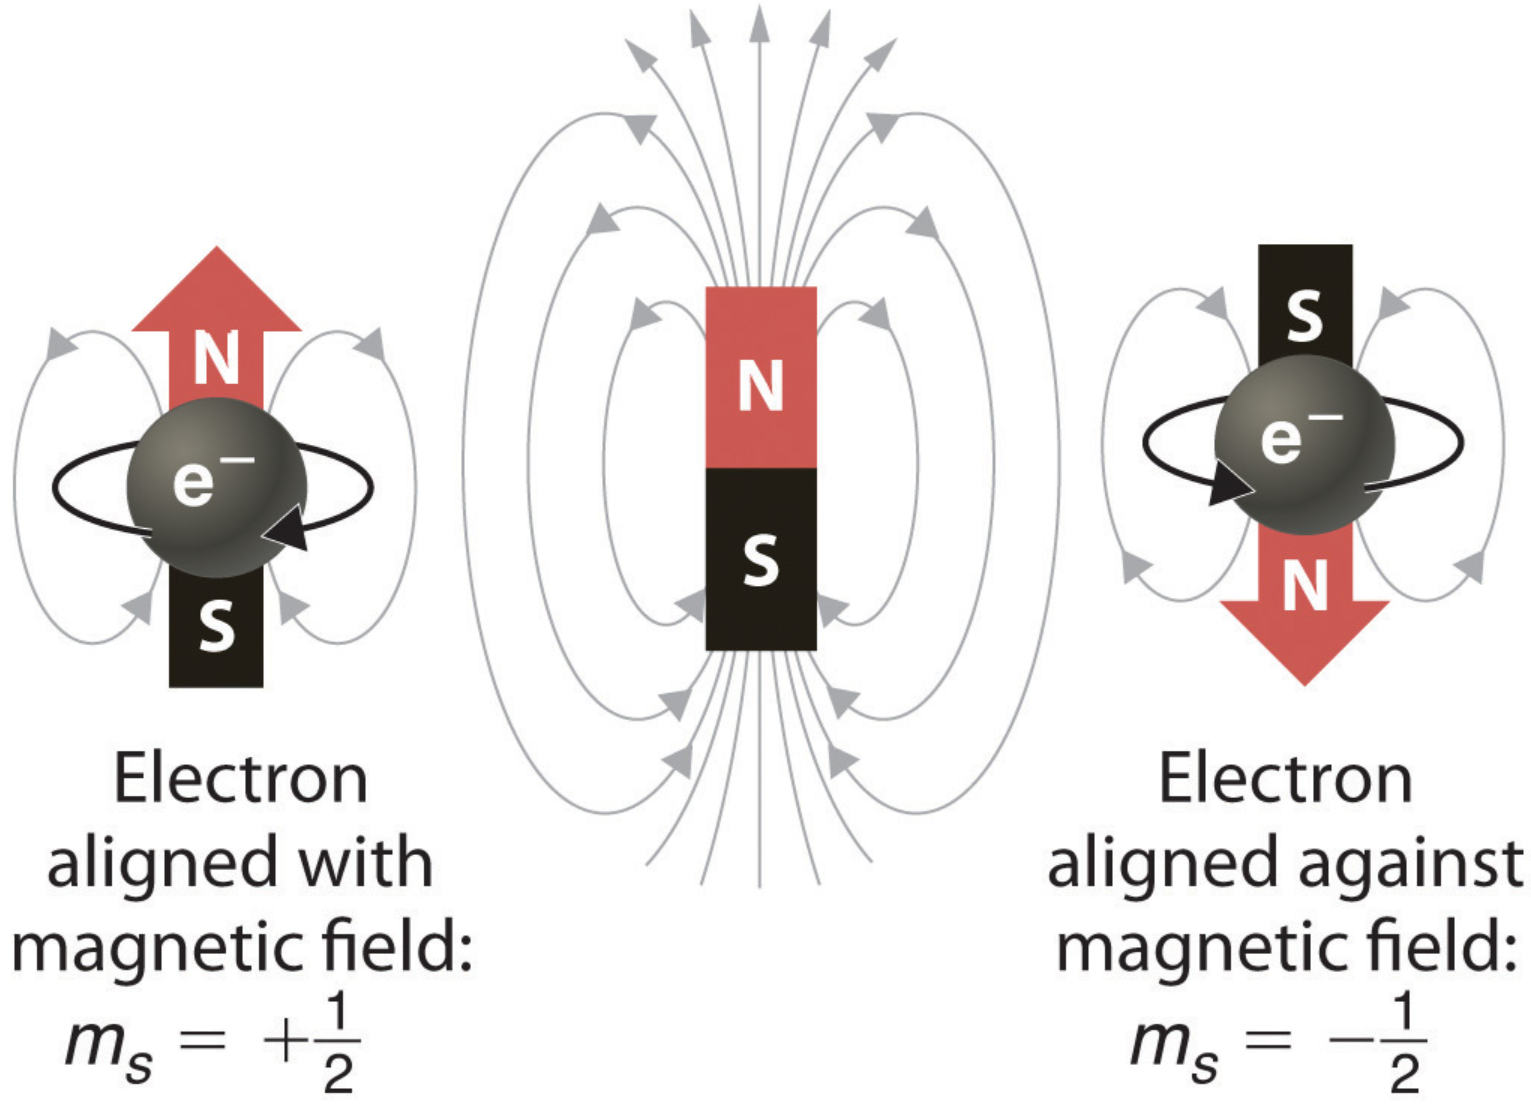
\includegraphics[width=0.5\textwidth]{Immagini_Micro&Nano/Imm_1_Ripasso/spin.png}
    \captionof{figure}{Lo spin di due elettroni in un livello orbitale deve essere opposto}
\end{center}
Questo significa che anche lo spin dell'elettrone è quantizzato ed è necessario introdurre un quarto numero quantico, il numero quantico di spin, che può assumere solo valore di $+\dfrac{1}{2}$ e $-\dfrac{1}{2}$
%
\subsubsection{Riempimento elettronico degli orbitali}
Sò che un atomo è composto da un nucleo circondato da uno o più elettroni, quello che voglio sapere ora è come gli elettroni si dispongono attorno. 
Per il riempimento degli atomi polielettronici vale il principio di esclusione di Pauli: in un atomo non possono esistere due elettroni aventi i quattro numeri quantici uguali. \\
Siccome un orbitale è caratterizzato da tre dei quattro numeri quantici, n, l, m, allora un orbitale può ospitare al massimo due elettroni che si differenziano per il numero quantico di spin, cioè che hanno spin antiparallelo.
%
\begin{exbox}

    %\captionof{figure}{Configurazione degli orbitali}
\begin{center}
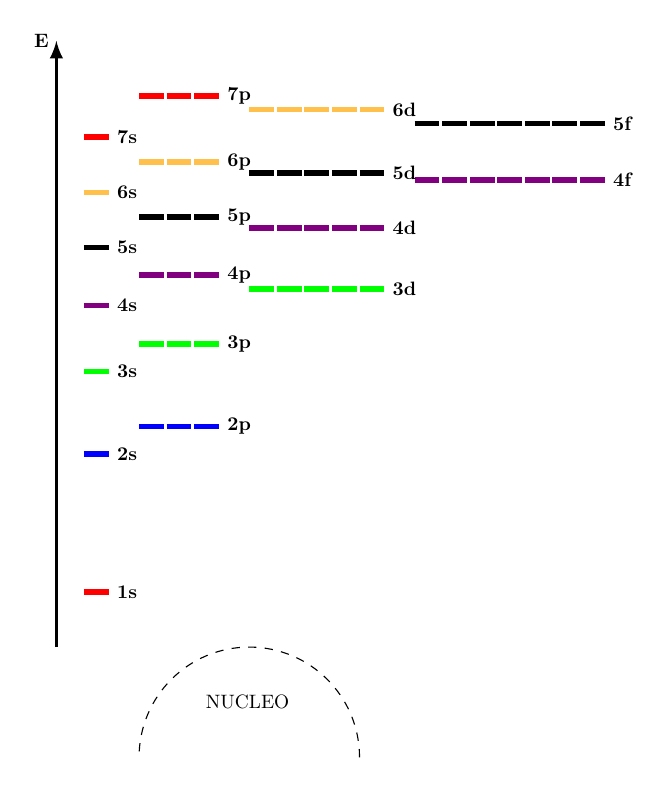
\begin{tikzpicture}[scale=0.7, transform shape]
    %disegno nucleo
    \draw[black, dashed] (5.5,-1) arc (0:180:2);
    \node at (4.35,0)[left]{NUCLEO};
    %disegno y
    \draw[-latex,very thick](0,1)--(0,12)node[left,black]{\textbf{E}};
    %disegno livello 1s
    \draw[line width=2pt,red](0.5,2)--++(0.45,0)node[right,black]{\textbf{1s}};
    %%%%%%%%%%%%%%%%%%%%%%%%%%%%%%%%%%%%%%%%%%%%%%%%%%%%%%%%%%%%%%%%%%%%%%%%%%
    %disegno livello 2s
    \draw[line width=2pt,blue](0.5,4.5)--++(0.45,0)node[right,black]{\textbf{2s}}
    %disegno livello 2p
    (1.5,5)--++(0.45,0) (2,5)--++(0.45,0) (2.5,5)--++(0.45,0)node[right,black]{\textbf{2p}};
    %%%%%%%%%%%%%%%%%%%%%%%%%%%%%%%%%%%%%%%%%%%%%%%%%%%%%%%%%%%%%%%%%%%%%%%%%%
    %disegno livello 3s
    \draw[line width=2pt,green](0.5,6)--++(0.45,0)node[right,black]{\textbf{3s}}
    %disegno livello 3p
    (1.5,6.5)--++(0.45,0) (2,6.5)--++(0.45,0) (2.5,6.5)--++(0.45,0)node[right,black]{\textbf{3p}}
    %disegno livello 3d
    (3.5,7.5)--++(0.45,0) (4,7.5)--++(0.45,0) (4.5,7.5)--++(0.45,0) (5,7.5)--++(0.45,0) (5.5,7.5)--++(0.45,0)node[right,black]{\textbf{3d}};
    %%%%%%%%%%%%%%%%%%%%%%%%%%%%%%%%%%%%%%%%%%%%%%%%%%%%%%%%%%%%%%%%%%%%%%%%%%
    %disegno livello 4s
    \draw[line width=2pt,violet](0.5,7.2)--++(0.45,0)node[right,black]{\textbf{4s}}
    %disegno livello 4p
    (1.5,7.75)--++(0.45,0) (2,7.75)--++(0.45,0) (2.5,7.75)--++(0.45,0)node[right,black]{\textbf{4p}}
    %disegno livello 4d
    (3.5,8.6)--++(0.45,0) (4,8.6)--++(0.45,0) (4.5,8.6)--++(0.45,0) (5,8.6)--++(0.45,0) (5.5,8.6)--++(0.45,0)node[right,black]{\textbf{4d}}
    %disegno livello 4f
    (6.5,9.47)--++(0.45,0) (7,9.47)--++(0.45,0) (7.5,9.47)--++(0.45,0) (8,9.47)--++(0.45,0) (8.5,9.47)--++(0.45,0) (9,9.47)--++(0.45,0) (9.5,9.47)--++(0.45,0)node[right,black]{\textbf{4f}};
    %%%%%%%%%%%%%%%%%%%%%%%%%%%%%%%%%%%%%%%%%%%%%%%%%%%%%%%%%%%%%%%%%%%%%%%%%%
    %disegno livello 5s
    \draw[line width=2pt,black](0.5,8.25)--++(0.45,0)node[right,black]{\textbf{5s}}
    %disegno livello 5p
    (1.5,8.8)--++(0.45,0) (2,8.8)--++(0.45,0) (2.5,8.8)--++(0.45,0)node[right,black]{\textbf{5p}}
    %disegno livello 5d
    (3.5,9.6)--++(0.45,0) (4,9.6)--++(0.45,0) (4.5,9.6)--++(0.45,0) (5,9.6)--++(0.45,0) (5.5,9.6)--++(0.45,0)node[right,black]{\textbf{5d}}
    %disegno livello 5f
    (6.5,10.5)--++(0.45,0) (7,10.5)--++(0.45,0) (7.5,10.5)--++(0.45,0) (8,10.5)--++(0.45,0) (8.5,10.5)--++(0.45,0) (9,10.5)--++(0.45,0) (9.5,10.5)--++(0.45,0)node[right,black]{\textbf{5f}};
    %%%%%%%%%%%%%%%%%%%%%%%%%%%%%%%%%%%%%%%%%%%%%%%%%%%%%%%%%%%%%%%%%%%%%%%%%%
     %disegno livello 6s
    \draw[line width=2pt,orange](0.5,9.25)--++(0.45,0)node[right,black]{\textbf{6s}}
    %disegno livello 6p
    (1.5,9.8)--++(0.45,0) (2,9.8)--++(0.45,0) (2.5,9.8)--++(0.45,0)node[right,black]{\textbf{6p}}
    %disegno livello 6d
    (3.5,10.75)--++(0.45,0) (4,10.75)--++(0.45,0) (4.5,10.75)--++(0.45,0) (5,10.75)--++(0.45,0) (5.5,10.75)--++(0.45,0)node[right,black]{\textbf{6d}};
    %%%%%%%%%%%%%%%%%%%%%%%%%%%%%%%%%%%%%%%%%%%%%%%%%%%%%%%%%%%%%%%%%%%%%%%%%%
     %disegno livello 7s
    \draw[line width=2pt,red](0.5,10.25)--++(0.45,0)node[right,black]{\textbf{7s}}
    %disegno livello 7p
    (1.5,11)--++(0.45,0) (2,11)--++(0.45,0) (2.5,11)--++(0.45,0)node[right,black]{\textbf{7p}};
    %\draw [arrows = {-Stealth[harpoon]}];
\end{tikzpicture}
\captionof{figure}{Configurazione degli orbitali}
\end{center}
   
%
    Consideriamo atmoni neutri non eccitati (detti allo stato fondamentale in cui elettroni non hanno energia sufficiente a fare salti) e sistemiamo gli elettroni seguendo lo schema di energie ed applicando il principio di Paoli.\\
    ES.1:\\
    L'idrogeno è un elemento con numero atomico Z=1. allora si ha un elettrone nell'orbitale 1s.\\
    ES.1:\\
    L'elio è un elemento con numero atomico Z=2. allora l'orbitale 1s sarà pieno.

    Facendo un passo in avanti, considero la regola di Hund: quando ci sono a disposizione più orbitali vuoti della stessa energia, gli elettroni vanno a occupare singolarmente questi orbitali con gli elettroni che anno a ruotare con spin parallelo.\\
    ES.3:\\
    Il carbonio (C) è un elemento con numero atomico Z=6. allora si ha due elettroni in due diversi orbitali 2p con spin parallelo.\\
    da mettere una figura con spin
\end{exbox}
%
\cleardoublepage
\section{Teoria delle bande e buche di potenziale}

Per sopravvivere dal baratro delle domande d'esame senza risposta, qui scrivo un riassunto che va ripetuto a pappagallo. Subito dopo c'è tutta una sezione dedicata alla spiegazione di codeste strane parole che sembrano messe a caso.

In un atomo isolato gli elettroni possono assumere solo determinati livelli energetici (E1, E2, E3..) che sono i risultati della soluzione dell'equazione di Schrödinger per quel sistema specifico. 

Quando invece un atomo è in presenza di tanti altri atomi dello stesso tipo (come in un reticolo cristallino), questi interagiscono tra loro causando la ramificazione dei livelli di energia formando più livelli con energi poco diverse tra loro, cioè una gamma di valori ammessi che prende il nome di banda di energia. Al posto di livelli discreti, si formano diverse bande.\\
In quest'ultimo caso, le buche di potenziale associate a ciascun nucleo danno luogo ad un potenziale periodico in cui le buche di potenziale corrispondono alla posizione degli atomi.
\subsection{Buca di potenziale in un atomo isolato}
%
Dalla Legge di Coulomb sò che l'energia potenziale tra due cariche è una funzione inversamente proporzionale alla loro distanza.
Considero quindi la struttura di un atomo, in particolare il suo nucleo ed un elettrone (prendiamo come esempio l'atomo di idrogeno). \\
Il sistema costituito da un protone e da un elettrone possiede una certa energia potenziale $U_p(r)$ che posso determinare attraverso la formula del campo elettrico tra due cariche, ottenendo:
\begin{equation*}
    \mathcal{E}(r)=\dfrac{1}{4\pi \epsilon_0} \dfrac{q}{r^2}=k \dfrac{q}{r^2}
\end{equation*}
con $k=\dfrac{1}{4\pi \epsilon_0}$ detta costante di Coulomb.\\
Il potenziale è dato da:
\begin{equation*}
    V(r)=\int_{r}^{\inf}\dfrac{kq}{r^2}dr=\dfrac{kq}{r}
\end{equation*}
dove si è posto la condizione $V(r)=0$ per $r\rightarrow \inf$.\\
Quindi trovo che l'energia potenziale dell'elettrone $U_p(r)$ è dato da:
\begin{equation*}
    U_p(r)=-qV(r)=-\dfrac{kq^2}{r}
\end{equation*}
l'andamento fisico per ($ r>0$) e l'andamento 3D saranno quindi:
\begin{figure}[htb!]
    \centering
    \begin{minipage}[b]{0.49\textwidth}
        \centering
        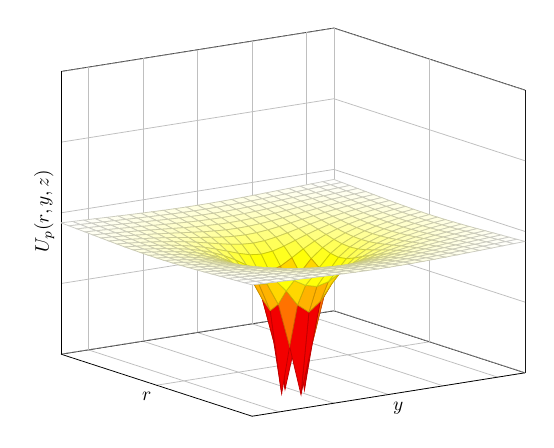
\begin{tikzpicture}[scale=0.7]
    \begin{axis}[
        xlabel={\(r\)},
        ylabel={\(y\)},
        ticks=none,
        zlabel={\(U_p(r,y,z)\)},
        view={55}{15},
        grid=major,
        xmin=-5,
        xmax=5,
        ymin=-5,
        ymax=5,
        zmin=-2,
        zmax=2,
    ]
    \addplot3[
        surf,
        domain=-5:5,
        domain y=-5:5,
        restrict z to domain=-8:1,
        colormap/hot2,
        shader=faceted,
    ] {-1/sqrt(max(x^2 + y^2, 0.01))};
    
    \end{axis}
        \end{tikzpicture}
        \caption{Buca di potenziale di un atomo isolato \\ in 3D}
        \label{fig:Buca di potenziale di un atomo isolato in 3D}
    \end{minipage}%
    \begin{minipage}[b]{0.49\textwidth}
        \centering
       \begin{tikzpicture}[scale=0.45]
        % disegno x
        \draw[->] (0,0) -- (10,0) node[below] {$r$};
        % disegno y
        \draw[->] (0,-5) -- (0,2) node[left] {$U_p(r)$};
        
        % Disegno la curva per r > 0
        \draw[red, domain=0.2:10, samples=100] plot (\x, {-1/\x});
    \end{tikzpicture}
    \caption{Buca di potenziale di un atomo isolato \\ in 2D}
    \label{fig:Buca di potenziale di un atomo isolato in 2D}
    \end{minipage}
    \caption{Buca di potenziale di un atomo isolato}
        \label{fig:Buca di potenziale di un atomo isolato}
\end{figure}
%
\\
Osservando il grafico 3D si può intuire come mai  hanno chiamato questo andamento "buca di potenziale".
Se prendo una sezione 2D avrò quello che molto speso si vede nei testi:
%
\begin{figure}[hbt!]
    \centering
    \includegraphics{Immagini_Micro&Nano/Imm_1_Ripasso/Andamento dell'energia potenziale in un atomo.png}
    \caption{Andamento dell'energia potenziale in un atomo}
    \label{fig:enter_label}
\end{figure}
%
\\
se $r$ è la distanza dell'elettrone dal nucleo dell'atomo allora posso capire che in $r=0$ è situato proprio il nucleodell'atomo.\\
Vedo quindi che per distanze piccole, l'elettrone è prigioniero della buca di potenziale fino a quando non assume abbastanza energia  da superare una soglia e guadagnare la libertà (aka: $U_e > U_{p}(r_1)$).\\
Una considerazione fondamentale in relazione alle buche di potenziale di un atomo siolato è la \textbf{quantizzazione dell'energia}. Questo principio deriva direttamente dall'equazione di Schrödinger e implica che l'energia in un sistema fisico è consentita solo in determinati livelli discreti. \\
Per capire meglio quest'ultima frase, di seguito ho posto una spiegazione. Siccome non sono fisico quantistico, ho trattato la buca di potenziale sotto opportune semplificazioni (visibili nella figura successiva) per affrontarla in maniera più semplice.
%

\begin{citbox}[solo per curiosità]
Si consideri il moto di una particella lungo l'asse $x$; in tale caso la funzione d'onda dipende solo dalla coordinata $x$ e pertanto l'equazione di
Schrédinger può ridursi ad una sola dimensione spaziale.
Si supponga che il moto
della particella non sia libero, ma piuttosto sia confinato da una buca di potenziale ideale di altezza infinita, ossia avvenga in un potenziale pari a 0 per $0<x<d$ e
tendente a $+\inf$ per $x < 0$ e $x > d$:
%
\begin{center}
    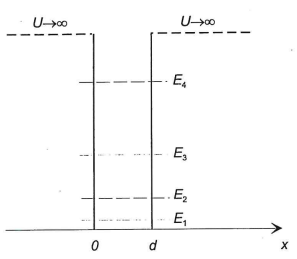
\includegraphics[width=0.25\textwidth]{Immagini_Micro&Nano/Imm_1_Ripasso/Buca di potenziale di altezza infinita.png}
    \captionof{figure}{Buca di potenziale infinita}
\end{center}
%
Poiché il potenziale non dipende
dal tempo si fa uso dell'equazione di Schrédinger per gli stati stazionari in
una dimensione: 
\begin{equation*}
    \dfrac{\hslash^2}{2m}\dfrac{d^2\psi}{dx^2}+(E-U)\psi(x)=0
\end{equation*}
Per risolvere questa equazione studiamo la buca di potenziale per ottenere le condizioni al contorno:
\begin{enumerate}
    \item Per $x<0$ ed $x>d$ l'energia potenziale $U \rightarrow \inf$. Questo si traduce in $\psi=0$, significa che al di fuori della regione della buca di potenziale, la probabilità di trovare la particella è zero. Pertanto, la funzione d'onda, che descrive la probabilità di trovare la particella in una data posizione, deve essere zero al di fuori della buca di potenziale.

    \item Per $0<x<d$ (all'interno della buca di potenziale) vale $U=0$
\end{enumerate}
Detto questo, per garantire la continuità delle funzioni d'onda, all'interno della buca di potenziale ($0<x<d$) dovrà valere $\psi(0)=\psi(d)=0$.
Poniamoci all'interno della buca ($0<x<d$ ed $U=0$), l'equazioni diventa:
\begin{align*}
    \dfrac{\hslash^2}{2m}\dfrac{d^2\psi}{dx^2}+E\psi(x)=0
\end{align*}
La soluzione generale sarà
\begin{equation*}
    \psi(x)=Asin(kx)+Bcos(kx)
\end{equation*}
dove $k=\sqrt{\dfrac{2mE}{\hslash^2}}$\\
Le costanti arbitrarie A e B si determinano imponendo le condizioni al contorno.
Da $\psi(0)=0$ si ottiene $B = 0$; imponendo poi $\psi(d)=0$ risalgo alla condizione $sin(kd)=0$ da cui:
\begin{equation*}
    k=\sqrt{\dfrac{2mE}{\hslash^2}}=\dfrac{n\pi}{d}
\end{equation*}
da cui 
\begin{equation*}
    E=\dfrac{n^2\hslash^2\pi^2}{2md^2}
\end{equation*}
In conclusione l'insieme delle energie permesse è numerabile, e tutte le energie permesse sono multipli interi di un livello fondamentale corrispondente an = 1. Le funzioni d'onda $A sin(kx)$ sono mostrate nella figura sopra . Si noti che a energie crescenti corrisponde un maggior numero di zeri della funzione d'onda (e quindi della probabilità)
all'interno della buca.\\
In generale, lo spettro è continuo in quelle situazioni in cui il moto della particella non
è confinato ad una regione finita dello spazio. Viceversa, lo spettro delle energie e discreto quando il moto della particella è in qualche modo confinato
\end{citbox}
%
\subsection{Buche di potenziale in un reticolo cristallino}
Un solido è formato da tanti atomi posti uno accanto all'altro e, come nel caso isolato, Il nucleo di ciascun atomo crea un campo elettrico ma la differenza è che adesso interagisce con quello degli atomi vicini.
Il risultato sarà che nel solido cristallino, l'energia potenziale creata dall'ammasso di atomi ha forma tridimensionale come nella figura seguente:
%
\begin{figure}[hbt!]
    \centering
    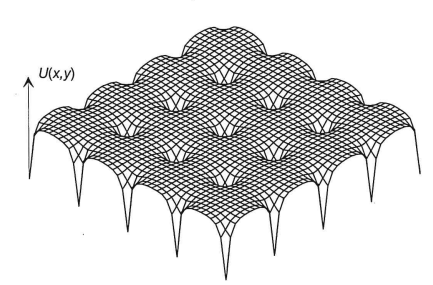
\includegraphics{Immagini_Micro&Nano/Imm_1_Ripasso/Potenziale periodico 3D.png}
    \caption{Potenziale periodico all'interno di un cristallo. 
}
    \label{fig:Potenziale periodico all'interno di un cristallo.}
\end{figure}
\\%
\textbf{La distanza tra due nuclei di due atomi è chiamato "1 Armstrong"}.\\
Come nel caso precedente prendiamo una sezione che passa attraverso i nuclei:
%
\begin{figure}[hbt!]
    \centering
    \includegraphics{Immagini_Micro&Nano/Imm_1_Ripasso/Andamento dell'energia potenziale in un solido.png}
    \caption{Andamento dell'energia potenziale in un solido}
    \label{fig: Andamento dell'energia potenziale in un solido}
\end{figure}
\\%
Dalla figura vedo che la curva non è più asintotica ma presenta un massimo posto a metà tra i due atomi (a metà armstrong).\\
Anche qui faccio delle approssimazioni che mi consentono di vedere le buche in una maniera più intuitiva:
%
FIGURA TA TOGLIERE E CAMBIARE QUELLA SOPRA USANDO LATEX
\begin{figure}[hbt!]
    \centering
    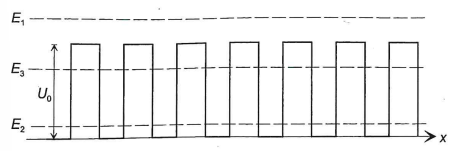
\includegraphics{Immagini_Micro&Nano/Imm_1_Ripasso/Potenziale periodico 2D.png}
    \caption{Potenziale periodico formato da una successione di buche di energia potenziale di altezza finita}
    \label{fig:Potenziale periodico formato da una successione di buche di energia potenziale di altezza finita}
\end{figure}
\\%
Un generico elettrone può trovarsi in diverse situazioni a seconda dell'energia che epossiede:
Io sò che una buca di potenziale può essere vista come un insieme discreto di energie e continue (?).\\
---------------------------------------------------------------------------------------------
Una particella stà all'interno della buca MA, A causa dell'effetto tunnel, le partigelle legate hanno probabilità finita di esistere anche all'esterno della buca.
Consideriamo ora una seconda buca di potenziale, identica, posta a distanza finita dalla prima. Il sistema risultante dalle due buche presenterà sempre un insieme di stati legati, le cui energie non coincideranno però con quelle della buca isolata a
causa del principio di esclusione, ma risulteranno dallo sdoppiamento di queste; vi
sarà poi sempre un insieme continuo di energie corrispondenti a particelle libere. 
...\\
...\\
...\\
----------------------------------------------------------------------------------------------
In una struttura periodica gli elettroni si possono trovare in tre tipi di situazioni:
\begin{enumerate}
    \item elettroni con energia ($E_1 > U_0$, che si muovono come nello spazio libero e non risentono (se non debolmente) della presenza delle buche di potenziale. Si dice che è nello stato libero;

    \item Particelle legate ($E_2 < U_0$, che hanno bassa probabilità di passare da una buca all'altra e pertanto restano confinate, rispettivamente all'interno della propria buca, in modo analogo a quanto accade nel caso di un atomo isolato. Si dice che è nello stato legato al nucleo (di uno degli atomi).

    \item Particelle quasi-libere ($E_3 \approx U_0$), che hanno la possibilità di muoversi per effetto tunnel da una buca di potenziale all'altra e quindi si comportano in modo simile ad una particella libera, ma con relazione fra energia totale $E$ e quantità di moto p diversa da quella della particella libera. Non vado ad indagare oltre (Guione pg 53)
\end{enumerate}
%
Gli elettroni del primo caso, chiamati elettroni liberi,  sono quelli che mi interessano poichè il loro moto forma la corrente elettrica quando vengono sottoposti all'azione di un campo elettrico esterno.\\
Possono quindi muoversi in regioni più distanti dal nucleo, ma continuano comunque ad essere influenzati dalla forza di attrazione elettrostatica con i rispettivi nuclei (ricordo che è una forza elastica).
%
\begin{psbox}[perchè gli elettroni liberi non escono dal solido? sono liberi di uscire dalla buca no?] \label{perchè gli elettroni liberi non escono dal solido?}
    Pur potendosi muovere all'interno del solido, gli elettroni non possono allontanarsene. Tutto funziona come se alla superficie del solido ci fosse una brusca variazione del potenziale che gli elettroni non possono superare se non possiedono la corrispondente energia.
\end{psbox} 
%
 Quando gli atomi si uniscono per formare un cristallo, i livelli energetici degli elettroni degli strati più interni non vengono apprezzabilmente alterati dalla presenza degli atomi vicini, mentre i livelli degli elettroni dell'orbita più esterna risultano cambiati considerevolmente, poichè questi elettroni in un cristallo sono condivisi da più di un atomo.\\
I nuovi livelli energetici degli elettroni esterni possono essere determinati per mezzo della meccanica quantistica e si trova che l'accoppiamento tra gli elettroni dello strato esterno (associato ai livelli d ed f) degli atomi porta come conseguenza la formazione una una banda di livelli energetici poco distanziati tra loro, al posto dei singoli livelli energetici fortemente spaziati presenti nel cso dell'atomo isolato
\begin{figure}[hbt!]
    \centering
    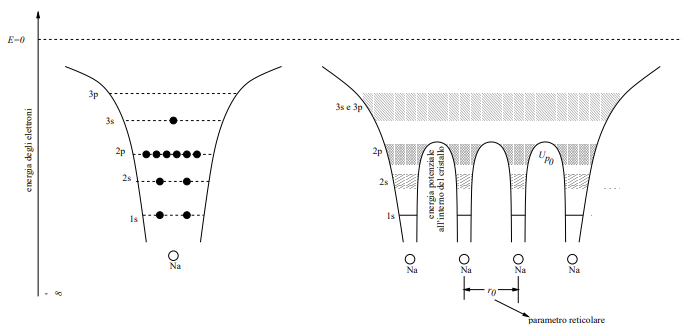
\includegraphics{Immagini_Micro&Nano/Imm_1_Ripasso/Bande di energie nel caso isolato VS solido.png}
    \caption{Livelli energetici nel caso di atomo isolato VS livelli energetici nel caso di un solido}
    \label{fig:Livelli energetici nel caso di atomo isolato VS livelli energetici nel caso di un solido}
\end{figure}
%
\\
Adesso voglio sapere come si formano le bande di energia.\\

consideriamo un sistema costituito da due soli atomi. 
Per entrambi gli atomi consideriamo solo l'elettrone che occupa il livello di energia più elevato (cioè quello più esterno; i chimici li chiamano d o f), trascurando i livelli occupati di energia inferiore.\\
Quando due atomi sono separati da una distanza così grande da poterli considerare isolati, l'elettrone associato a ciascun atomo possiede un'energia di valore $E_n$ soluzione dell'equazione di Schrodinger (spiegato prima).\\
Se la distanza di separazione è ridotta, un elettrone sarà soggetto a una forza dovuta alla presenza del secondo nucleo. Il potenziale che determina i livelli di energia dell'elettrone risulta quindi modificato e così pure lo spettro dei possibili valori di energia. Per descrivere un sistema di due atomi devo usare il principio di esclusioen di paoli. In condizioni normali ogni atomo isolato ha un livello di energia En che può ospitare al massimo due elettroni con spin opposto, limitando il sistema a un massimo di quattro elettroni.
%
\begin{psbox}[l'ultima frase è spiegata male]
    Nel caso di un singolo atomo isolato, un livello di energia (denotato come En) può ospitare al massimo due elettroni, ciascuno con spin opposto. Quindi, se prendiamo due atomi isolati, il numero massimo di elettroni che possono occupare il livello En è 4 (2 nel primo atomo e 2 nel secondo).
    RIVERE QUESTA SEZIONE
\end{psbox}
%
 Tuttavia, quando i due atomi si avvicinano a formare un unico sistema, il livello di energia consentito En può ora ospitare solo due elettroni. Quindi il livello di energia En relativo a ciascun atomo isolato si sdoppierà in due livelli, di energia leggermente differente, al fine di garantire la coesistenza di quattro elettroni.\\
L'effetto dell'iterazione tra i due atomi è di perturbare il valore di energia relativo al livello considerato dell'atomo isolato e di indurreuno sdoppiamento dei livelli di energia perturbati.\\
Avvicinando ulteriormente i due atomi, la perturbazione dovuta all'avvicinamento è maggiore, come pure la differenza di energia tra i livelli sdoppiati.\\
Raggruppando più atomi di una struttura scristallina, le forze cui sono soggetti gli elettroni sono ulteriormente modificate e così pure i valori di energia permessi.\\
---------------\\
Anche qui, il principio di esclusione di Pauli richiede che
ciascun livello permesso abbia un'energia di valore leggermente diverso, cosicchè il cristallo risulta caratterizzato
da numerosi livelli, tutti distinti in energia ma molto prossimi tra loro. Ogni livello quantizzato corrispondente
all'atomo isolato si scinde in più livelli, ciascuno corrispondente a un atomo nel sistema. Se il sistema è composto
da N atomi, l'originario livello di energia En si scinde in N livelli permessi, costituenti una banda di energia
che contiene al più 2N elettroni.\\ 
Poichè il numero di atomi in un cristallo è molto grande (dell'ordine di $10^{22} cm^{-3}$) e l'estensione della banda di energia è dell'ordine di pochi eV, gli N livelli distinti componenti le bande sono separati da intervalli di energia assai più piccoli dell'energia termica di un elettrone a temperatura ambiente, cosicchè l'elettrone può agevolemnte effettuare transizioni tra i livelli. Si può quindi parlare di una banda continua di valori di energia permessi, occupabile al più da 2N elettroni.
%
\begin{figure}[hbt!]
    \centering
    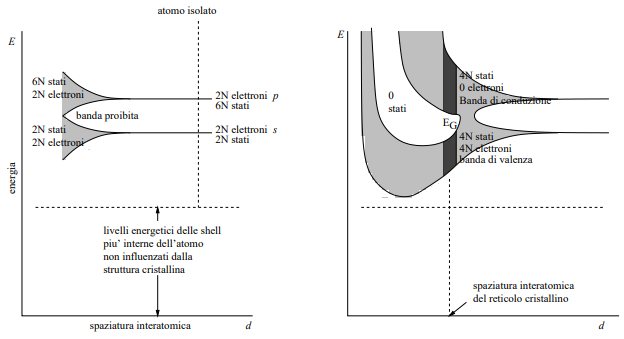
\includegraphics{Immagini_Micro&Nano/Imm_1_Ripasso/bande di energia.png}
    \caption{Banda di energia che si forma in un reticolo cristallino}
    \label{fig:Banda di energia che si forma in un reticolo cristallino}
\end{figure}
%

Quindi i livelli discreti di energia-dell'atomo isolato si trasformano in bande di energia permessa separate da bande proibite.\\
Le bande di energia interessanti ai fini del comportamento-chimico ed elettrico sono quelle superiori: la banda contenente gli elettroni di valenza, quelli cioè più esterni, che contribuiscono
ai legami chimici, è detta banda di valenza mentre la banda immediatamente superiore si dice banda di conduzione. \\
Si può assumere come estremo superiore della banda di conduzione il livello del vuoto; al livello del vuoto corrisponde l'energia minima che un elettrone deve possedere per sfuggire all'esterno del solido. Per energie maggiori del livello del vuoto l'elettrone è libero e la sua energia presenta uno spettro continuo. All'interno di ciascuna banda (valenza o conduzione) la relazione di dispersione dell'elettrone si può in molti casi approssimare con una forma parabolica analoga alla relazione di dispersione di un elettrone
nello spazio libero; la relativa massa efficace m* si indicherà con m;, per gli elettroni della banda di conduzione e con —mj, per gli elettroni della banda di valenza,
per motivi che diventeranno chiari in seguito. \\

La buca di potenziale è una zona di spazio circondata da un elevato campo elettrico. in un atomo gli elettroni dell'atomo vedono il nucleo posto al centro di una buca di potenziale.
%
\subsection{Dentro la lezione di microelettronica: struttura a bande}
La sezione precedente aveva lo scopo di spiegare dando un'idea di quello che succede nel reticolo cristallino e servirà anche per rispondere a dubbi che si creeranno leggendo questa sezione.\\
Qui rifaremo le medesime osservazioni ma sotto opportune semplificazioni visive per rendere il problema matematicamente trattabile.\\

All'interno della bucha di potenziale, un elettrone ha la possibilità di muoversi liberamente. Tuttavia, se l'elettrone acquista abbastanza energia cinetica e si allontana notevolmente dal centro dell'atomo, può superare la forza di attrazione e, di conseguenza, "uscire" dalla regione di influenza dell'atomo.\\
Questo fenomeno può essere spiegato attraverso i principi della meccanica quantistica, in cui la posizione dell'elettrone è descritta dalla funzione d'onda e la sua probabilità di trovarsi in diverse posizioni è governata dalle leggi della teoria quantistica.\\

Le buche di potenziale più esterne dal reticolo cristallino vengono rappresentate con pareti di potenziale infinite (vedi sezione \ref{perchè gli elettroni liberi non escono dal solido?}) mentre ciascuna delle buche interne al solido può essere modellata come come una buca di potenziale con con pareti limitate non infinite, dove la parete della buca di potenziale di un atomo viene chiusa dalla parete della buca di potenziale dell'atomo accanto (vedi Figura \ref{fig: Andamento dell'energia potenziale in un solido}):

\begin{figure}[htb!]
    \centering
    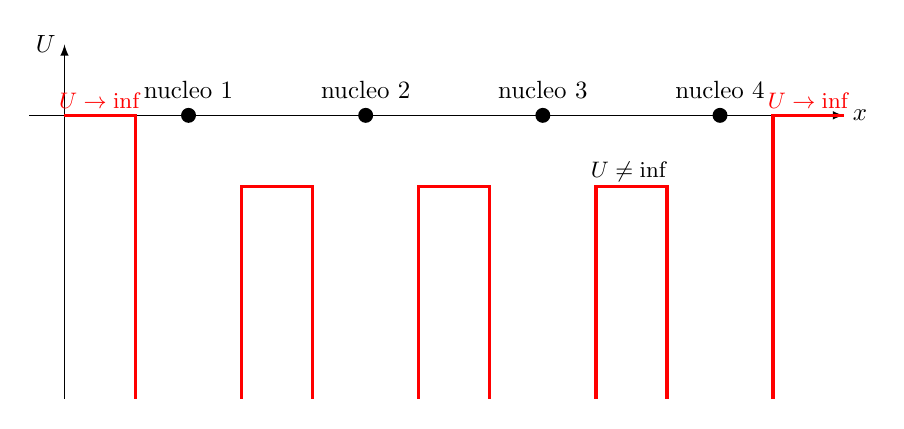
\begin{tikzpicture}[scale=0.9, transform shape]
        %disegno asse x
        \draw[-latex] (-0.5,0)-- (11,0) node[right]{$x$};
        %disegno asse y
        \draw[-latex] (0,-4)-- (0,1) node[left]{$U$};
        %disegno buche e label potenziale
        \draw[very thick,red] (0,0)--++ (1,0)--++ (0,-4);
        \draw[very thick,red] (2.5,-4)--++ (0,3)--++ (1,0)--++ (0,-3);
        \draw[very thick,red] (5,-4)--++ (0,3)--++ (1,0)--++ (0,-3);
        \draw[very thick,red] (7.5,-4)--++ (0,3)--++ (1,0)--++ (0,-3);
        \draw[very thick,red] (10,-4)--++ (0,4)--++ (1,0);
        \node at (-0.2,0.2)[right,red]{\small{$U\rightarrow \inf$}};
        \node at (9.8,0.2)[right,red]{\small{$U\rightarrow \inf$}};
        \node at (7.97,-0.8)[thick]{\small{$U \neq \inf$}};
        %disegno i nuclei 
        \node[circle,fill=black,inner sep=0pt,minimum size=6pt,label=nucleo 1] at (1.75,0) {};
        \node[circle,fill=black,inner sep=0pt,minimum size=6pt,label=nucleo 2] at (4.25,0) {};
        \node[circle,fill=black,inner sep=0pt,minimum size=6pt,label=nucleo 3] at (6.75,0) {};
        \node[circle,fill=black,inner sep=0pt,minimum size=6pt,label=nucleo 4] at (9.25,0) {};
       
    \end{tikzpicture}
    \caption{Buche di potenziale in un solido-Le più esterne hanno pareti con potenziale infinito}
    \label{fig:Buche di potenziale in un solido-Le più esterne hanno pareti con potenziale infinito}
\end{figure}
%
\noindent\begin{minipage}{0.6\textwidth}% adapt widths of minipages to your needs
Ricordo che se la parete di potenziale è infinita, i livelli energetici ammessi sono discreti e di valore:
\begin{equation*}
    E_n=\dfrac{n^2\hslash^2 \pi^2}{2md}
\end{equation*}
dove d è la distanza tra le pareti della buca.
Si noti come l'energia dipende solo dalla distanza tra le pareti mentre \textbf{l'altezza della buca non entra in gioco} perchè l'altezza della buca è infinita.
Se le pareti fossero finite (\textbf{aka: $U \neq \inf$}), si otterrebbero dei livelli che vanno come:
\begin{equation*}
    E_u=n^2h\pi^2
\end{equation*}
\end{minipage}%
\hfill%
\begin{minipage}{0.3\textwidth}
\begin{center}
    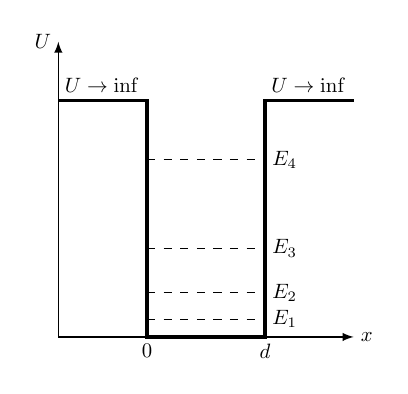
\begin{tikzpicture}[scale=0.75,transform shape]
        %disegno asse x
        \draw[-latex] (0,0)-- (5,0) node[right]{$x$};
        %disegno asse y
        \draw[-latex] (0,0)-- (0,5) node[left]{$U$};
        %disegno buche
        \draw[very thick,black] (0,4)--++ (1.5,0) node[anchor=south east]{$U\rightarrow \inf$} --++ (0,-4)--++ (2,0)--++ (0,4)--++ (1.5,0) node[anchor=south east]{$U\rightarrow \inf$};
        %livelli energetici
        \draw[dashed] (1.5,0.30)--++ (2,0) node[right]{$E_1$};
        \draw[dashed] (1.5,0.75)--++ (2,0) node[right]{$E_2$};
        \draw[dashed] (1.5,1.5)--++ (2,0) node[right]{$E_3$};
        \draw[dashed] (1.5,3)--++ (2,0) node[right]{$E_4$};
        %label
        \node at (1.5,0)[below]{$0$};
        \node at (3.5,0)[below]{$d$};
    \end{tikzpicture}
    \captionof{figure}{buca di potenziale con pareti infinite}
    \label{fig:buca di potenziale con pareti infinite}
\end{center}
\end{minipage}
Nel caso di pareti finite è più difficile trovare i valori in forma chiusa dei livelli di energia discreti (E1,E2,E3..) ma la cosa più importante è un'altra:
Nelle buche di potenziale a pareti infinite, la probabilità di trovare un elettrone all'interno della buca di potenziale ha una funzione d'onda $\psi_1, \psi_2,\psi_3$ tale per cui 
\begin{equation}
    \sum_i \int \left| \psi_i\right|^2 dx=1
\end{equation}
\\%
Questa cosa la posso tradurre come "nel caso infinito ho che per x<0 e x>d ho probabilità nulla fuori dalla buca e probabilità certa dentro la buca".\\
Nel caso di pareti finite la situazione cambia dato che si può osservare una probabilità diversa da zero che di trovare l'elettrone fuori e \textbf{questo è il concetto proveniente dalla meccanica quantistica che ci portiamo dietro}.\\
%
\noindent\begin{minipage}{0.49\textwidth}% adapt widths of minipages to your needs
\begin{center}
    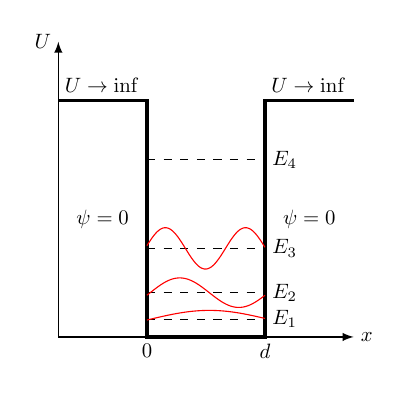
\begin{tikzpicture}[scale=0.75,transform shape]
        %disegno asse x
        \draw[-latex] (0,0)-- (5,0) node[right]{$x$};
        %disegno asse y
        \draw[-latex] (0,0)-- (0,5) node[left]{$U$};
        %disegno buche
        \draw[very thick,black] (0,4)--++ (1.5,0) node[anchor=south east]{$U\rightarrow \inf$} --++ (0,-4)--++ (2,0)--++ (0,4)--++ (1.5,0) node[anchor=south east]{$U\rightarrow \inf$};
        %livelli energetici
        \draw[dashed] (1.5,0.30)--++ (2,0) node[right]{$E_1$};
        \draw[dashed] (1.5,0.75)--++ (2,0) node[right]{$E_2$};
        \draw[dashed] (1.5,1.5)--++ (2,0) node[right]{$E_3$};
        \draw[dashed] (1.5,3)--++ (2,0) node[right]{$E_4$};
        %label
        \node at (1.5,0)[below]{$0$};
        \node at (3.5,0)[below]{$d$};
        %plot funzioni psi
        \draw[red, domain=1.5:3.5, samples=200, smooth] plot (\x, {0.3+0.15*sin(90*\x+220))});
        \draw[red, domain=1.5:3.5, samples=200, smooth] plot (\x, {0.75+0.25*sin(180*\x+80))});
        \draw[red, domain=1.5:3.5, samples=200, smooth] plot (\x, {1.5+0.35*sin(265*\x-30))});
        %
        \node at (0.75,2)[align=center]{$\psi = 0$};
        \node at (4.25,2)[align=center]{$\psi = 0$};
        \end{tikzpicture}
    \captionof{figure}{buca di potenziale con pareti infinite, l'elettrone è confinato nella buca}
    \label{fig:buca di potenziale con pareti infinite v2}
\end{center}
\end{minipage}%
\hfill%
\begin{minipage}{0.49\textwidth}
\begin{center}
    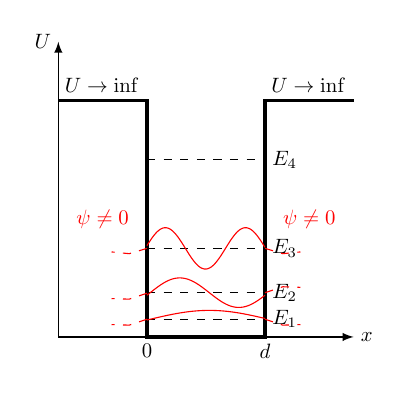
\begin{tikzpicture}[scale=0.75,transform shape]
        %disegno asse x
        \draw[-latex] (0,0)-- (5,0) node[right]{$x$};
        %disegno asse y
        \draw[-latex] (0,0)-- (0,5) node[left]{$U$};
        %disegno buche
        \draw[very thick,black] (0,4)--++ (1.5,0) node[anchor=south east]{$U\rightarrow \inf$} --++ (0,-4)--++ (2,0)--++ (0,4)--++ (1.5,0) node[anchor=south east]{$U\rightarrow \inf$};
        %livelli energetici
        \draw[dashed] (1.5,0.30)--++ (2,0) node[right]{$E_1$};
        \draw[dashed] (1.5,0.75)--++ (2,0) node[right]{$E_2$};
        \draw[dashed] (1.5,1.5)--++ (2,0) node[right]{$E_3$};
        \draw[dashed] (1.5,3)--++ (2,0) node[right]{$E_4$};
        %label
        \node at (1.5,0)[below]{$0$};
        \node at (3.5,0)[below]{$d$};
        %plot funzione psi E1
        \draw[red,dashed] (1.5,0.3)--++ (-0.3,-0.1)--++ (-0.3,0.01);
        \draw[red, domain=1.5:3.5, samples=200, smooth] plot (\x, {0.3+0.15*sin(90*\x+220))});
        \draw[red,dashed] (3.5,0.3)--++ (0.3,-0.1)--++ (0.3,0.01);
        %plot funzione psi E2
         \draw[red,dashed] (1.5,0.74)--++ (-0.3,-0.1)--++ (-0.3,0.01);
        \draw[red, domain=1.5:3.5, samples=200, smooth] plot (\x, {0.75+0.25*sin(180*\x+80))});
        \draw[red,dashed] (3.5,0.75)--++ (0.3,+0.1)--++ (0.3,-0.01);
        %plot funzione psi E3
         \draw[red,dashed] (1.5,1.5)--++ (-0.3,-0.09)--++ (-0.3,0.03);
        \draw[red, domain=1.5:3.5, samples=200, smooth] plot (\x, {1.5+0.35*sin(265*\x-30))});
        \draw[red,dashed] (3.5,1.5)--++ (+0.3,-0.09)--++ (+0.3,0.03);
        %
        \node at (0.75,2)[align=center,red]{$\psi \neq 0$};
        \node at (4.25,2)[align=center,red]{$\psi \neq 0$};
    \end{tikzpicture}
    \captionof{figure}{buca di potenziale con pareti finite, non è detto che l'elettrone sia confinato nella buca}
    \label{fig:buca di potenziale con pareti finite}
\end{center}
\end{minipage}
\\%
Da qui si scatena un'altro ragionamento:
Io sò che per ogniuno di questi livelli energetici (e1, e2...) il principio di esclusione di paoli sancisce che due elettroni non possono avere lo stesso stato energetico a meno che non abbiano spin opposto.\\
Allora succede che nel momento in cui atomi isolati cominciano ad unirsi formando il reticolo cristallino, elettroni che appartengono a buche adiacenti hanno probabilità diversa da zero di esistere nei livelli energetici degli atomi accanto.
Se nucleo 1 ha 1 elettrone e nucleo 3 ha un altro elettrone, allora la probabilità di trovare questi due dentro il nucleo 2 è diversa da zero.
Questo è legato al fatto che siccome le buche non hanno pareti infinite, allora la funzione d'onda si espande fuori dalla buca.
\begin{figure}[htb!]
    \centering
    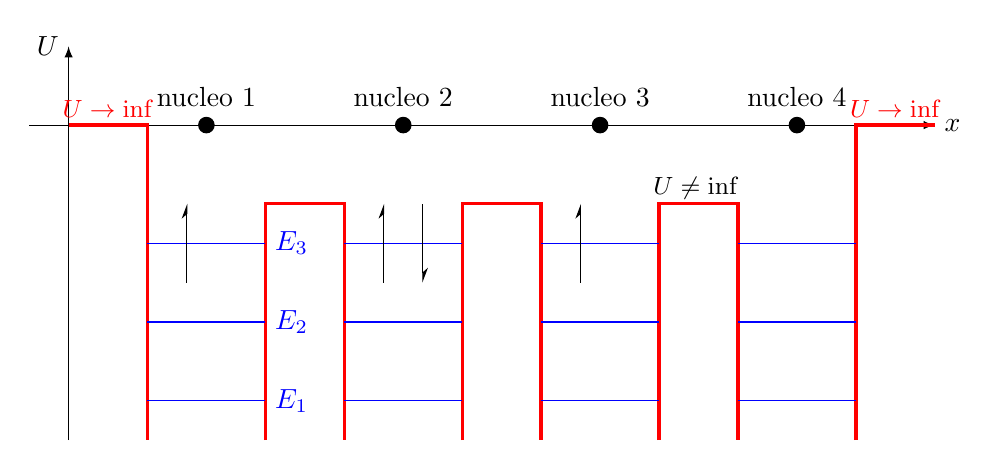
\begin{tikzpicture}
        %disegno asse x
        \draw[-latex] (-0.5,0)-- (11,0) node[right]{$x$};
        %disegno asse y
        \draw[-latex] (0,-4)-- (0,1) node[left]{$U$};
        %disegno buche e label potenziale
        \draw[very thick,red] (0,0)--++ (1,0)--++ (0,-4);
        \draw[very thick,red] (2.5,-4)--++ (0,3)--++ (1,0)--++ (0,-3);
        \draw[very thick,red] (5,-4)--++ (0,3)--++ (1,0)--++ (0,-3);
        \draw[very thick,red] (7.5,-4)--++ (0,3)--++ (1,0)--++ (0,-3);
        \draw[very thick,red] (10,-4)--++ (0,4)--++ (1,0);
        \node at (-0.2,0.2)[right,red]{\small{$U\rightarrow \inf$}};
        \node at (9.8,0.2)[right,red]{\small{$U\rightarrow \inf$}};
        \node at (7.97,-0.8)[thick]{\small{$U \neq \inf$}};
        %disegno i nuclei 
        \node[circle,fill=black,inner sep=0pt,minimum size=6pt,label=nucleo 1] at (1.75,0) {};
        \node[circle,fill=black,inner sep=0pt,minimum size=6pt,label=nucleo 2] at (4.25,0) {};
        \node[circle,fill=black,inner sep=0pt,minimum size=6pt,label=nucleo 3] at (6.75,0) {};
        \node[circle,fill=black,inner sep=0pt,minimum size=6pt,label=nucleo 4] at (9.25,0) {};
        %disegno livelli energetici
        \draw[blue] (1,-3.5)--++ (1.5,0) node[right]{$E_1$};
        \draw[blue] (1,-2.5)--++ (1.5,0) node[right]{$E_2$};
        \draw[blue] (1,-1.5)--++ (1.5,0) node[right]{$E_3$};
        %%%%
        \draw[blue] (3.5,-3.5)--++ (1.5,0) ;
        \draw[blue] (3.5,-2.5)--++ (1.5,0) ;
        \draw[blue] (3.5,-1.5)--++ (1.5,0) ;
        %%%%
        \draw[blue] (6,-3.5)--++ (1.5,0) ;
        \draw[blue] (6,-2.5)--++ (1.5,0) ;
        \draw[blue] (6,-1.5)--++ (1.5,0) ;
        %%%%
        \draw[blue] (8.5,-3.5)--++ (1.5,0) ;
        \draw[blue] (8.5,-2.5)--++ (1.5,0) ;
        \draw[blue] (8.5,-1.5)--++ (1.5,0) ;
        %disegno spin elettroni
        \draw[arrows = {-Stealth[harpoon]}] (1.5,-2)--++ (0,1);
        %%
        \draw[arrows = {Stealth[harpoon]-}] (4.5,-2)--++ (0,1);
        \draw[arrows = {-Stealth[harpoon]}] (4,-2)--++ (0,1);
        %%
        \draw[arrows = {-Stealth[harpoon]}] (6.5,-2)--++ (0,1);
    \end{tikzpicture}
    \caption{Buche di potenziale, livelli energetici ed elettroni}
    \label{fig:Buche di potenziale, livelli energetici ed elettroni}
\end{figure}
Questo fenomeno spiega anche l'origine dell'effetto tunnel. 1.30
%
\begin{figure}[htb!]
    \centering
    \begin{tikzpicture}
        %disegno asse x
        \draw[-latex] (-0.5,0)-- (5,0) node[right]{$x$};
        %disegno asse y
        \draw[-latex] (0,-0.5)-- (0,6) node[left]{$U$};
        %disegno barriera di potenziale
        \draw[] (2,0)rectangle++ (2,5) node[pos=.5,align=center]{barriera di \\potenziale};
        %incidente
        \draw[-stealth,decorate,decoration={snake,amplitude=3pt,pre length=2pt,post length=3pt}] (0.5,4) -- ++ (1.25,0);
        %trasmessa
        \draw[-stealth,decorate,decoration={snake,amplitude=3pt,pre length=2pt,post length=3pt}] (4.5,2.5) -- ++ (1.25,0);
        %riflessa
        \draw[stealth-,decorate,decoration={snake,amplitude=3pt,pre length=2pt,post length=3pt}] (0.5,1) -- ++ (1.25,0);
    \end{tikzpicture}
    \caption{Caption}%
    \label{fig:enter_label}
\end{figure}
effetto tunnel 1.31\\
allo stesso modo un elettrone parte di una buca può diventare parte di una buca adiacente. elettroni in una 1 e 3 possono trovarsi in buca 2 insieme a quello nativo. in totale sono 3 elettroni in buca due con una certa probabilità diversa da zero.
ALLORA E3 degenera.
il principio di paoli è mantenuto.
Graficamente, per descrivere l'andamento dell'energia in funzione della costante reticolare L si scopre che:
se atomi posti a distanza grande\\
\begin{figure}
    \centering
    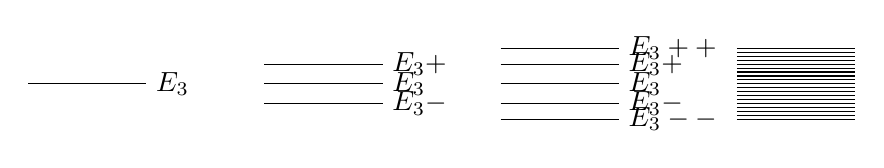
\begin{tikzpicture}
        \draw[] (0,0)--++ (1.5,0) node[right]{$E_3$};
        %
        \draw[] (3,0.25)--++ (1.5,0) node[right]{$E_3+$};
        \draw[] (3,0)--++ (1.5,0) node[right]{$E_3$};
        \draw[] (3,-0.25)--++ (1.5,0) node[right]{$E_3-$};
        %
        \draw[] (6,0.45)--++ (1.5,0) node[right]{$E_3++$};
        \draw[] (6,0.25)--++ (1.5,0) node[right]{$E_3+$};
        \draw[] (6,0)--++ (1.5,0) node[right]{$E_3$};
        \draw[] (6,-0.25)--++ (1.5,0) node[right]{$E_3-$};
        \draw[] (6,-0.45)--++ (1.5,0) node[right]{$E_3--$};
        %
        \draw[] (9,0.45)--++ (1.5,0);
        \draw[] (9,0.40)--++ (1.5,0);
        \draw[] (9,0.35)--++ (1.5,0);
        \draw[] (9,0.30)--++ (1.5,0);
        \draw[] (9,0.25)--++ (1.5,0);
        \draw[] (9,0.20)--++ (1.5,0);
        \draw[] (9,0.15)--++ (1.5,0);
        \draw[] (9,0.1)--++ (1.5,0);
        \draw[] (9,0.05)--++ (1.5,0);
        \draw[] (9,0)--++ (1.5,0);
        \draw[] (9,-0.45)--++ (1.5,0);
        \draw[] (9,-0.40)--++ (1.5,0);
        \draw[] (9,-0.35)--++ (1.5,0);
        \draw[] (9,-0.30)--++ (1.5,0);
        \draw[] (9,-0.25)--++ (1.5,0);
        \draw[] (9,-0.20)--++ (1.5,0);
        \draw[] (9,-0.15)--++ (1.5,0);
        \draw[] (9,-0.1)--++ (1.5,0);
        \draw[] (9,-0.05)--++ (1.5,0);
    \end{tikzpicture}
    \caption{Degenerazione del livello discreto fino a formare una banda}
    \label{fig:Degenerazione del livello discreto fino a formare una banda}
\end{figure}
----------\\
Un elettrone che indice sull abarriera di potenziale ad un'energia inferiore 
1.46\\
%
\cleardoublepage%
la forma d'onda delle funzioni soluzione dell'equazione di shrodinger + di tipo onda piana.\\
\begin{equation}
    \psi(x)= A\cdot \exp{[-jkx]} \text{, con \,\,\, } k=\sqrt{\dfrac{2mE}{h^2}}
\end{equation}
%
\begin{ripasso}[cos'è un onda piana?]
Prima di tutto consiglio di usare 3-D Wave Simulation per "vedere" le onde.\\
     Un'onda piana è caratterizzata da un profilo costante nel tempo, il che significa che \textbf{IL MODULO} dell'ampiezza dell'onda è costante lungo tutto il suo periodo. \\
     %
Un esempio che descrive questa condizione è:
\begin{equation}
    y(t)=A \cdot e^{j(wt+\phi)}
\end{equation}
L'equazione descrive un'onda piana complessa con modulo costante pari ad A. 
%
visivamente:
\begin{center}
    \begin{minipage}{0.49\textwidth}
        \centering
        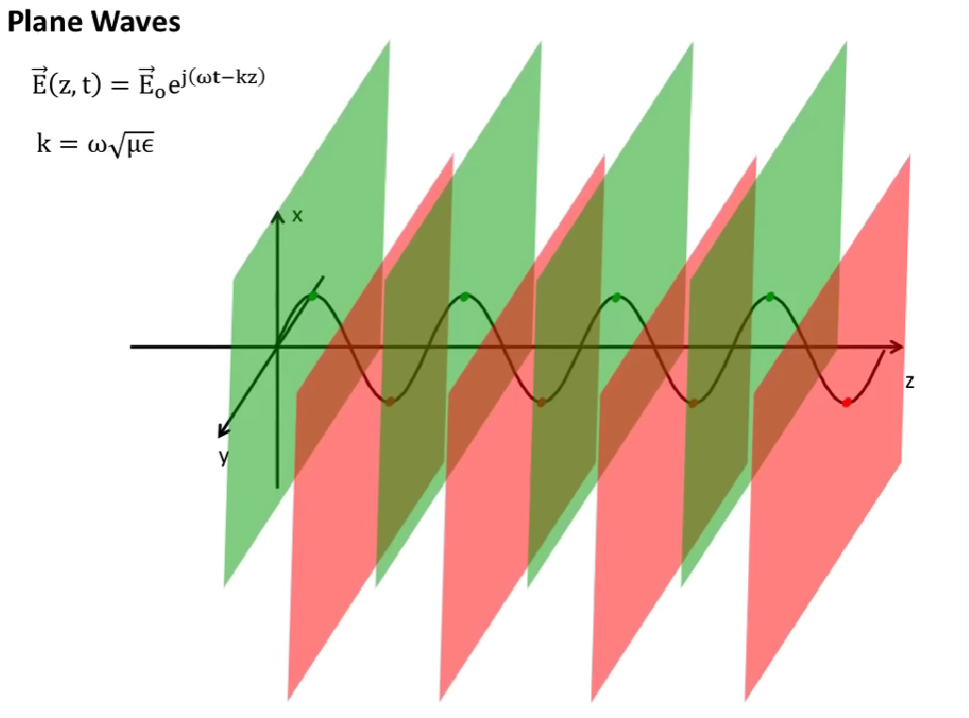
\includegraphics[width=0.85\textwidth]{Immagini_Micro&Nano/Imm_1_Ripasso/rappresentazione di onda piana.png}
        \captionof{figure}{Caption} % Use captionof here
        \label{fig:label1}
    \end{minipage}
    \hfill
    \begin{minipage}{0.49\textwidth}
        \centering
        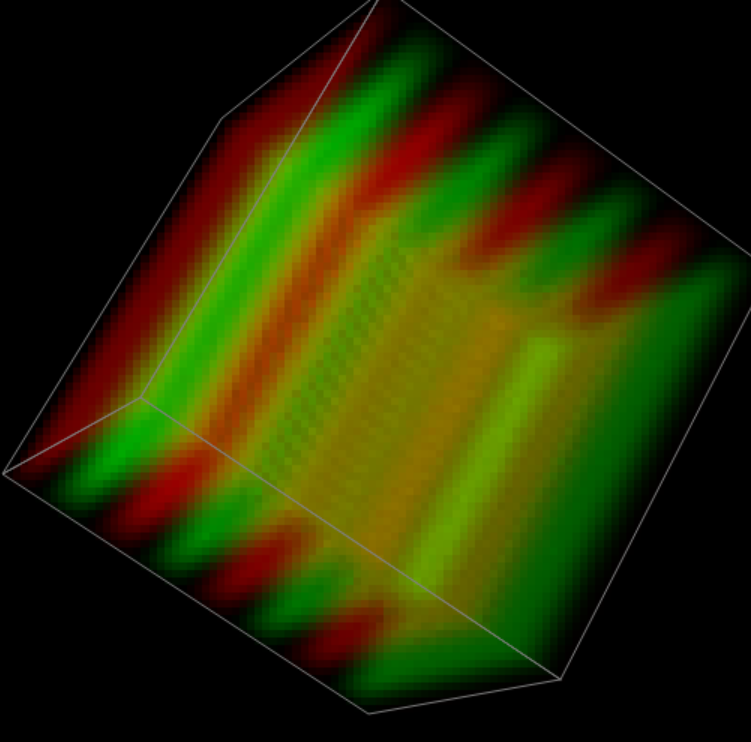
\includegraphics[width=0.65\textwidth]{Immagini_Micro&Nano/Imm_1_Ripasso/rappresentazione 3D onda piana.png}
        \captionof{figure}{Caption} % Use captionof here
        \label{fig:label2}
    \end{minipage}
\end{center}

\end{ripasso}
%
Come descritto nella sezione precedente.
%
\begin{psbox}
%
il pezzo qui sotto è da chiedere a ricevimento. è corretto?
\end{psbox}
Considero una particella in un sistema descritto dalle leggi della meccanica classica (Fisica I), una particella ha un'energia totale E data da:
\begin{equation*}
    E = E_{cinetica}+ E_{potenziale} = K + U
\end{equation*}
Se la particella ha energia totale $E > U_0$  allora si deduce che l'energia cinetica è maggiore di zero, infatti:
\begin{equation*}
    K+U > U \quad =>\quad K>U-U=0
\end{equation*}
La condizione $K>0$ viene intesa (o interpretata) come la capacità dell'elettrone muoversi liberamente sia all'interno (?????ricevimento) che all'esterno della buca di potenziale.\\
La condizione $E < U$ presenta una situazione duale alla precedente: l'elettrone è confinato all'interno della barriera di potenziale.\\
%
In questo contesto la meccanica classica mi aiuta a pensare all'elettrone come un oggetto semplice: sotto cerce condizioni può essere legata alla buca oppure libera da essa (aka: dentro o fuori alla buca).\\
%
Dal punto di vista quantistico la situazione è più complessa poichè la particella è vincolata alla buca, ma esiste comunque la probabilità non nulla che essa si trovi all'esterno della buca.\\
%
la funzione d'onda è ovunque di tipo oscillatorio e supponendo la condizione $E>U_0$, oppure $E \gg U_0$, si trascura l'energia potenziale $U_0$ dall'equazione di Schrodinger:
\begin{equation}
    \dfrac{d^2 \psi(x)}{dx^2} \approx -\dfrac{2mE}{\hslash^2}\psi(x)
\end{equation}
La sua soluzione è:
\begin{equation}
    \psi(x)= \psi^+ \cdot e^{-jkx} + \psi^-\cdot e^{+jkx} \text{, con } k=\sqrt{\dfrac{2mE}{h^2}}
\end{equation}
%
\begin{figure}[htb!]
    \centering
    \begin{tikzpicture}
        %disegno asse x
        \draw[-latex] (-0.5,0)-- (5,0) node[right]{$x$};
        %disegno asse y
        \draw[-latex] (0,-0.5)-- (0,4) node[left]{$U$};
        %disegno barriera di potenziale
        \draw[] (2,0)rectangle++ (1,3) node[pos=.5,align=center]{barriera di \\potenziale};
        %incidente
        \draw[-stealth,decorate,decoration={snake,amplitude=3pt,pre length=2pt,post length=3pt}] (0.5,2.5) -- ++ (1.25,0);
        %trasmessa
        \draw[-stealth,decorate,decoration={snake,amplitude=3pt,pre length=2pt,post length=3pt}] (3.5,1.75) -- ++ (1.25,0);
        %riflessa
        \draw[stealth-,decorate,decoration={snake,amplitude=3pt,pre length=2pt,post length=3pt}] (0.5,1) -- ++ (1.25,0);
    \end{tikzpicture}
    \caption{Caption}%
    \label{fig:enter_label}
\end{figure}
Cioè la funzione d'onda $\psi$ è la somma di due onde piane (una che si propaga verso destra, l'altra verso sinistra); 
inoltre l'energia E può assumere un valore qualsiasi.\\
In presenza di una buca di potenziale, soluzioni dell'equazione di Schròdinger oscillatorie in una regione illimitata dello spazio possono esistere per un insieme centinuo di valori dell'energia (eventualmente appartenente ad un insieme di intervalli); tali soluzioni vengono dette STATI NON LEGATI\\
\\
pg 33 \\
\\
Nel caso di $0<E<U$ l'equazione di shrodinger cambia forma e come risultato si ottiene una funzione d'onda psi a parte reale:
\begin{equation}
    \psi(x)= A\cdot \exp{[-\alpha x]}
\end{equation}
Dove $\alpha=\sqrt{\dfrac{2m(U-E)}{h^2}}$
La funzione d'onda $\psi(x)$ quindi non è più una funzione complessa  e questo è grazie al fatto che k è divento puramente immaginario:
\begin{equation}
    k=\sqrt{\dfrac{2m(E-U)}{h^2}}
\end{equation}
È chiaro che solo per alcuni particolari valori
dell'energia E la funzione d'onda soddisfa alle
condizioni al contorno. In conclusione:
In presenza di una buca di potenziale, soluzioni dell'equazione di
Schrodinger oscillatorie in una regione limitata dello spazio ed evanescenti alirove possono esistere solo per un insieme numerabile di valori dell'energia totale; tali soluzioni vengono dette, stati legati.

questa nuova equazione ci dice che si propaga come onda evanascente (grafico)\\
...\\
1.56
siccome la struttura è periodica, c'è un teorema che dice che $\psi$ è effettivamente un'onda piana però è moltiplicato per un termine che tiene conto della periodicità
\begin{equation}
    \psi(x)=\exp{[-jkx]} \cdot U_k(x)
\end{equation}
Dove $U_k$ è detta funzione d'onda periodica che dipende dalla periodicità degli stati.\\
come si analizza cosa succede all'interno della struttura periodica?\\
grafico\\
Considero zona I e zona II individualmente, come se non fossero pate di un periodo. strutture a parte con le loro equazioni di shrodinger.
la funzione risolta nel primo periodo (Nella zona "I") è:
\begin{equation}
    U_{kI}=A \cdot cos(\beta x) + B \cdot sen(\beta x) \text{, con \,\,\, } \beta=\sqrt{\dfrac{2mE}{h^2}}
\end{equation}
mentre nel secondo periodo (nella zona "II"), l'energia è minore di quella della barriera di potenziale.
Questo allora significa che la funzione non è più periodica perchè deve essere evanescente:
\begin{equation}
    U_{kII}=C \cdot cosh(\alpha x) + D \cdot senh(\alpha x) \text{, con \,\,\, } \beta=\sqrt{\dfrac{2mE}{h^2}}
\end{equation}
%
\\
quindi io ho diviso il mio sistema in 2 pezzi:
 vuoto + barriera con E<U\\
Per trovare la soluzione dell'eq di shrodinger devo raccordare le soluzione dei sottproblemi, cioè impongo le condizioni di contorno.
\begin{enumerate}
    \item $U_{kI}(0) = U_{kII}(0)$
    \item $U_{kI}'(0) = U_{kII}'(0)$
    \item $U_{kI}(a) = U_{kII}(-b)$
    \item $U_{kI}'(a) = U_{kII}'(-b)$
\end{enumerate}
Le condizioni 1) e 2) garantiscono al continuità della funzione e della sua derivata nel punto 0 mentre le condizioni 3) e 4) garantiscono la continuità della funzione e della sua derivata agli astremi.\\
Unendo la prima condizione all'equazione di $U_{kI}$ trovo che
\begin{equation*}
    A=C
\end{equation*}
Dalla seconda condizione al contorno trovo 
\begin{equation*}
    B \cdot \beta = D \cdot \alpha
\end{equation*}
Dalla terza condizione al contorno trovo 
\begin{equation*}
    A \cdot cos(\beta \,a) + B\cdot sen (\beta \,a)= e^{-jkL}\cdot \left[ C \cdot cosh(\alpha \,b)+D \cdot senh(\alpha \,b) \right]
\end{equation*}
Infine, dalla quarta condizione al contorno trovo 
\begin{equation*}
    -A\beta \cdot sen(\beta \,a) + B\beta \cdot sen(\beta \,a)= e^{-jkL}\cdot \left[ C\alpha \cdot senh(\alpha \,b)+D\alpha \cdot cosh(\alpha \,b) \right]
\end{equation*}
Queste equazioni messe insieme formano un sistema lineare omogeneo nelle incognite ABCD
\begin{alignat*}{4}
    A&=B \\
    %
    B &\cdot \beta = D \cdot \alpha \\
    %
    A &\cdot cos(\beta \,a) + B\cdot sen (\beta \,a)= e^{-jkL}\cdot \left[ C \cdot \cosh(\alpha \,b)+D \cdot senh(\alpha \,b) \right] \\
    %
    -A&\beta \cdot sen(\beta \,a) + B\beta \cdot sen(\beta \,a)= e^{-jkL}\cdot \left[ C\alpha \cdot senh(\alpha \,b)+D\alpha \cdot cosh(\alpha \,b) \right]
\end{alignat*}
%
\\
Ma a me non interessa il valore di queste quattro incognite, tuttavia voglio scartare la soluzione banale del sistema che si ottiene nella condizione di termini tutti nulli.\\
matrice e cose\\
ponendo il determinante della matrice diverso da zero significa imporre che il vettore $[A B C B] \neq 0$ e questo ci permette di trovare i livelli di energia ammessi.\\
Il determinante di questa matrice assume forma:
\begin{equation}
    \dfrac{\alpha^2-\beta^2}{2\,\alpha \beta}\cdot senh(\alpha \,a)+cosh(\alpha \,b)+senh(\beta \,a)=cosh(k \,L)
\end{equation}
Quest'equazione è ancora complicata, allora faccio un'altra ipotesi\\
\textbf{HP:}immaginiamo una barriera infinitamente alta e infinitamente sottile: $U_0 \rightarrow \inf $, $b \rightarrow 0$.
Si perviene, quindi, ad una forma dell'equazione più semplice:
\begin{equation}
    F(\beta a)=\underbrace{\dfrac{P}{\beta \, a}\cdot sen(\beta \,a)+cos(\beta \,a)}_{\text{non è detto che sia} -1<\cdot<1} = \underbrace{cos(ka)}_{-1<\cdot<1}
\end{equation}
dove $\beta$ contiene l'energia.
Solo quando "$\beta \cdot a$" è sufficientemente grande il primo termine è compreso tra -1 ed 1 e quindi c'è soluzione, altrimenti per certi valori può succere che non esiste un corrispondente valore di k reale.\\
 ma siccome k (che è una costante di propagazione) è proporzionale alla quantità di moto (hk=p)
e soprattuto dentro beta c'è energia, vuoldire che quel valore di k e di energia non sono compatibili con la soluzione del nostr problema.
questo si traduce nella seguente situazione:
%
\begin{figure}[hbt!]
    \centering
    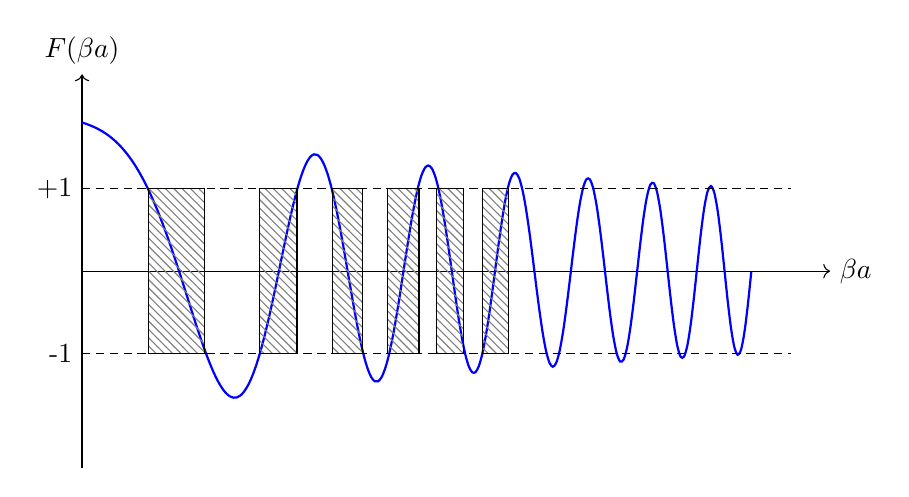
\begin{tikzpicture}[scale=1]
      % Axes
      \draw[->] (0.5,0) -- (10,0) node[right] {$\beta a$};
      \draw[->] (0.5,-2.5) -- (0.5,2.5) node[above] {$F(\beta a)$};
    
      % Sinusoidal graph with amplitude and frequency inversely proportional to x
      \draw[blue, thick, domain=0.5:9, samples=200, smooth] plot (\x, {20*cos(30*\x^2)/(\x+10))});
      %tratteggi
      \draw[densely dashed] (0.5,1.05)--++ (9,0);
      \draw[densely dashed] (0.5,-1.05)--++ (9,0);
      %sezioni rettangolari
      \draw[ pattern=north west lines, pattern color=gray] (1.345,-1.05) rectangle (2.06,1.05);
      \draw[ pattern=north west lines, pattern color=gray] (2.75,-1.05) rectangle (3.23,1.05);
      \draw[ pattern=north west lines, pattern color=gray] (3.68,-1.05) rectangle (4.06,1.05);
      \draw[ pattern=north west lines, pattern color=gray] (4.38,-1.05) rectangle (4.78,1.05);
      \draw[ pattern=north west lines, pattern color=gray] (5,-1.05) rectangle (5.35,1.05);
      \draw[ pattern=north west lines, pattern color=gray] (5.59,-1.05) rectangle (5.92,1.05);
      %label
      \node at (0.5,1.05)[left]{+1};
      \node at (0.5,-1.05)[left]{-1};
    \end{tikzpicture}
    \caption{Caption}%
    \label{fig:enter_label}
\end{figure}
\\%
ad un certo punto F(beta) sarà tutta dentro -1 ed 1.
solo allora esisterà un valore di k legato a quel particolare valore di beta e quindi ad un corrispondente valore di energia.\\
Nelle altre zone k è complesso ma allora $\psi$ che moltiplica tutta la funzione d'onda del cristallo diventa evanescente (vàa  0) e quindi nel semiconduttore non ci possono stare elettroni per quelle energie.\\
beta, energia e k sono legate ma \\
dire beta oppure energia è lo stesso ma k è la costante di propagazione nel vuoto (come se elett fosse onda piana), beta è la velocità di propagazione nel cristallo mentre k è la quantità di moto associata a...\\
k è legato alal quantità di moto dell'elettrone.
beta è legato all'energia.

\begin{equation}
    h \cdot k = p
\end{equation}
beta dipende da E
Posso scrivere un andamento che mi lega l'energia E a k\\
GRAFICO\\
\begin{exbox}[NOTA]
    
\end{exbox}

\section*{28/09/2023}
Descrivendo graficamente il legame tra energia e $k\dfrac{a}{\pi}$ (dove k è normalizzato rispetto a $\dfrac{a}{\pi}$), ottengo la seguente figura:
\begin{figure}[hbt!]
    \centering
    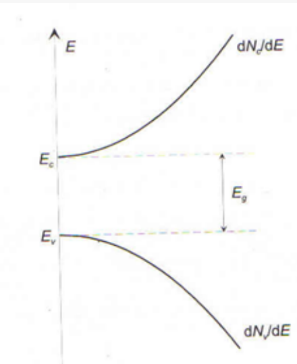
\includegraphics{Immagini_Micro&Nano/Imm_2_Fisica_dei_semiconduttori/densità di stati.PNG}
    \caption{Caption}%
    \label{fig:enter_label}
\end{figure}
%
\begin{figure}[hbt!]
    \centering
    \begin{tikzpicture}
        %disegno asse x
        \draw[->] (-3.5,0)-- (3.5,0) node[right] {$k\dfrac{a}{\pi}$};
        %disegno asse y
        \draw[->] (0, -0.5) -- (0, 4) node[above] {$\mathcal{E}(k)$};
        %disegno grafico
        \draw[scale=0.5, domain=-4.5:4.5, smooth, variable=\x, red]  plot ({\x},{-0.1*\x*\x + 3} );
        \draw[scale=0.5, domain=-4.5:4.5, smooth, variable=\x, red]  plot ({\x},{0.1*\x*\x + 5} );
        %disegno tratteggi verticali
        \draw[densely dotted] (-2.25,0) node[below]{$-1$}--++ (0,4);
        \draw[densely dotted] (2.25,0) node[below]{$+1$}--++ (0,4);
        %disegno tratteggi orizzontali
        \draw[densely dashed] (-3,0.5)--++ (6,0);
        \draw[densely dashed] (-3,1.5)--++ (6,0);
        %labels
        \node at (-0.01,3.5) [align=center]{banda di \\ conduzione};
        \node at (-0.01,0.5) [align=center]{banda di \\ valenza};
    \end{tikzpicture}
    \caption{Grafico di dispersione}
    \label{fig:Grafico di dispersione}
\end{figure}\\
%
Nei precedenti paragrafi ho detto che all'interno di un SC gli elettroni possiedono dell'energia e quindi hanno uno stato energetico.
%
\begin{psbox}[se l'elettrone ha energia ZERO?]
"Se l'elettrone ha energia nulla significa che non si muove, ma questa particolare condizione non esiste in meccanica quantistica poichè in questo ambito si considera che ogni particella abbia sempre dell'energia, per quanto piccola possa essere".\\
Gli elettroni quindi possono avere proprietà cinematiche a cui si associa un valore di energia e di quantità di moto.\\
%
\textbf{In realtà questa spiegazione è un riassunto inaccurato del principio di indeterminazione di Heisenberg}.\\
Il principio di indeterminazione afferma che è impossibile conoscere contemporaneamente e con precisione la posizione e la quantità di moto di una particella e quindi non è possibile assegnare con precisione un valore esatto all'energia della una particella in un dato istante di tempo.\\
Quindi negli elettroni, in realtà, ci sarà sempre una certa quantità di incertezza associata all'energia e quindi non possiamo mai dire che abbiamo energia nulla. 
\end{psbox}
%
Bisogna però fare una differenza tra cinematica classica e cinematica nei semiconduttori:\\
Nella meccanica classica l'energia cinetica e la quantità di moto di un corpo con massa $m$ sono legate l'una all'altra, da cui si trova che l'energia ha un andamento di tipo quadratico.
%
\begin{figure}[hbt!]
    \centering
    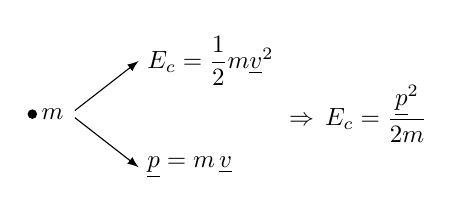
\begin{tikzpicture}[scale=0.9,transform shape]
        \filldraw[fill=black, thick] (0,0) circle (0.05) node[right]{$m$};
        \draw[-latex] (0.6,0.05)-- (1.5,0.75) node[right]{$E_c=\dfrac{1}{2}m\underline{v}^2$};
        \draw[-latex] (0.6,-0.05)-- (1.5,-0.75) node[right]{$\underline{p}=m \, \underline{v}$};
        \node at (3.5,0)[right]{$\Rightarrow \, E_c=\dfrac{\underline{p}^2}{2m} $};
    \end{tikzpicture}
\end{figure}\\

%
Gli elettroni nei semiconduttori invece, presentano una relazione tra energia e vettore k (contenuta all'interno della funzione $\psi$), quest'ultimo contenuto anche nella quantità di moto di un elettrone $p=\hslash k$. trovare le equazione corrette nella figura
\begin{figure}[hbt!]
    \centering
    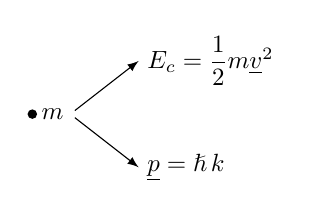
\begin{tikzpicture}[scale=0.9,transform shape]
        \filldraw[fill=black, thick] (0,0) circle (0.05) node[right]{$m$};
        \draw[-latex] (0.6,0.05)-- (1.5,0.75) node[right]{$E_c=\dfrac{1}{2}m\underline{v}^2$};
        \draw[-latex] (0.6,-0.05)-- (1.5,-0.75) node[right]{$\underline{p}=\hslash \, k$};
    \end{tikzpicture}
\end{figure}\\

 Tale relazione và a costruire la figura iniziale, chiamata diagramma di dispesione e rappresenta la relazione dell'energia in funzione di k.\\
 ------------------------------\\
La sua natura corpuscolare viene meno in favore della natura ondulatoria da quis i ha il diagramma di dispersione.??????\\
 ------------------------------\\
In pratica, dentro il semiconduttore, io non posso più considerare energia e quantità di moto legate come se fossi nella meccanica classica ed inoltre io sò che gli elettroni esistono in delle fasce di energia ammissibili. \\
min9.09\\
l'andamento è mostrato in figura ??\\
Perciò, in un primo momento, penserei di fare un miscuglio di formule analitiche, ovvero di considerare la legge della cinematica classica e buttarci dentro il valore della quantità di moto della particella ($\underline{p}$) che fa parte "del mondo quantistico", ottenendo:

\begin{equation}
    E_c=\dfrac{p^2}{2m}=\dfrac{\hslash^2k^2}{2m}
\end{equation}

Ma nel caso quantistico non c'è un legame tra E e k di tipo quadratico poichè il diagramma di dipersione mostra un andamento non quadratico e quindi l'equazione precedente poichè non descrive correttamente tutto l'andamento.\\
Tuttavia posso fare l'approssimazione di $k$ sufficientemente piccolo ($k \approx 0$) in modo da semplificare l'andamento del diagramma di dispersione come fosse di tipo parabolico e quindi rendere valida l'equazione:
\begin{equation}
    E=\dfrac{\hslash^2 k^2}{2m}
\end{equation}
\textbf{Devo tenere in considerazione che $k$ piccolo è sinonimo di quantità di moto ed energia basse}.
Tale approssimazione è mostrata in figura:
\begin{figure}[hbt!]
    \centering
    \begin{tikzpicture}
        %disegno asse x
        \draw[->] (-3.5,0)-- (3.5,0) node[right] {$k$};
        %disegno asse y
        \draw[->] (0, -0.5) -- (0, 4) node[above] {$\mathcal{E}$};
        %disegno grafici rossi
        \draw[scale=0.5, domain=-4.5:4.5, smooth, variable=\x, red]  plot ({\x},{-0.1*\x*\x + 3} );
        \draw[scale=0.5, domain=-4.5:4.5, smooth, variable=\x, red]  plot ({\x},{0.1*\x*\x + 5} );
        %disegno grafici verdi
        \draw[scale=0.5, domain=-1.65:1.65, smooth, variable=\x, green!50!black]  plot ({\x},{-0.75*\x*\x + 3} );
        \draw[scale=0.5, domain=-1.65:1.65, smooth, variable=\x, green!50!black]  plot ({\x},{0.75*\x*\x + 5} );
        %disegno tratteggi verticali
        \draw[densely dotted] (-2.25,0) node[below]{$-1$}--++ (0,4);
        \draw[densely dotted] (2.25,0) node[below]{$+1$}--++ (0,4);
        %disegno tratteggi orizzontali
        \draw[densely dashed] (-3,0.5)--++ (6,0);
        \draw[densely dashed] (-3,1.5)--++ (6,0);
    \end{tikzpicture}
    \caption{Grafico di dispersione vero(rosso) ed approssimato(verde)}
    \label{fig:Grafico di dispersione vero ed approssimato}
\end{figure}\\
%
quindi $E=\dfrac{\hslash^2 k^2}{2m}$ è l'equazione che si avrebbe nello spazio libero ma non dentro al SC, se non per k piccoli.
Questo implica che su ogni banda, l'energia in funzione di k è data dalla somma dell'energia in $k=0$ + un "termine correttivo" che serve per descrivere l'andamento vero dell'energia quando k non è piccolo:
\begin{equation}
    \left. E(k)\right |_{k\rightarrow 0} \approx  \underbrace{\underbrace{E(k=0)}_{\text{andamento approssimato}} + \, \, \dfrac{\hslash k^2}{2m^*}}_{\text{andamento reale}}
\end{equation}
$m^*$ è chiamata massa efficace ed ha la dimensione di una massa. Questo parametro è l'elemento chiave nell'equazione perchè dovrò sceglierlo in maniera opportuna in modo che la somma totale mi rappresenti il vero diagramma (con ammessi piccoli errori) in un range tale per cui k è piccolo.
\begin{psbox}
    Un processo simile ( ma assolutamente non uguale) l'ho studiato a campi elettromagnetici con la teoria di Sommerfield. l'antenna in presenza di terreno può essere studiata come antenna in presenza di piano PEC (ideale) + un termine correttivo che tende a 0 per $\sigma \rightarrow \inf$.\\

    Questo non ha nulla a che fare con quanto detto ma è giusto per similitudine:\\
    \[E = E_{ideale}+E_{correttivo}\]
    dove $E_{correttivo}$ è il termine correttivo che tente a 0 per $k \rightarrow 0$.\\
    Se ci pensi il valore ideale sarebbe l'equazione della meccanica classica:)
\end{psbox}
La massa efficace è un numero il cui valore dipende dalla banda in cui si trova l'elettrone (dipende cioè dall'energia della particella) e quindi, per ottenere un corretto andamendo del grafico di dispersion,  dovrò associare all'elettrone in banda di conduzione la massa $m_n^*+$ e dòvrò associare all'elettrone in banda di valenza la massa $m_n^*-$. \\
C'è però una piccola osservazione da fare. in banda di valenza l'energia è data dal movimento delle lacune, ovvero "alla mancanza dell' elettrone" e quindi è a queste lacune che io associerò la massa in banda di valenza: $m_h^*-$ .\\

E' importante ricordare che questa massa non ha nulla a che fare con la vera massa degli elettroni e delle lacune in quanto è uno stratagemma matematico che noi abbiamo adottato per approssimare il diagramma di dispersione con la forma tipica dell'energia nello spazio libero.
\begin{figure}
    \centering
    \begin{tikzpicture}
        %disegno asse x
        \draw[->] (-0.5,0)-- (3.5,0) node[right] {$k$};
        %disegno asse y
        \draw[->] (0, -0.5) -- (0, 4) node[above] {$\mathcal{E}$};
        %disegno grafici verdi
        \draw[scale=0.5, domain=-1.65:1.65, smooth, variable=\x, green!50!black]  plot ({\x+2.5},{-0.75*\x*\x + 3} );
        \draw[scale=0.5, domain=-1.65:1.65, smooth, variable=\x, green!50!black]  plot ({\x+2.5},{0.75*\x*\x + 5} );
        %label
        \node at (1.4,3.5)[]{$m_n^*+$};
        \node at (1.4,0.5)[]{$m_h^*-$};
    \end{tikzpicture}
    \caption{Caption}%
    \label{fig:enter_label}
\end{figure}
-\\
Non solo le masse efficaci dovranno avere valori opportuni (sicuramente diversi tra loro) ma dovranno avere anche segno opposto. Infatti, osservando il diagramma di distribuzione, si  vede che una parabola è rivolta vero l'altro e l'altra è rivolta verso il basso e pertanto sceglierò $m_n^*+ >0$ per gli elettroni in banda di conduzione e $m_h^*-<0$ per quelle in banda di valenza.\\
Il segno delle masse efficaci quindi dipende dal fatto che si stia considerando banda di conduzione o di valenza ma il loro modulo è inversamente proporzionale alla curvatura del campo elettrico del diagramma di dispersione.\\
Se la curvatura è maggiore allora avrò bisogno di una massa efficace minore e viceversa.
riassumento:
\begin{itemize}
    \item in BC avrò una $m_n^* >0$
    \item in BV avrò una $m_h^* <0$
\end{itemize}
\begin{tikzpicture}[overlay]
    \node at (5.5,1.15)[right]{con};
    \node at (6.5,1.55)[right]{$|m_n|$};
    \node at (6.5,0.75)[right]{$|m_h|$};
    \node at (7.5,1.15)[right]{$1/\alpha \,\, \dfrac{d^2E(k)}{dk^2}$};
\end{tikzpicture}
Quello che si scopre nella pratica è che 
\begin{equation}
    \left | m_n^* \right | < \left | m_h^* \right | 
\end{equation}
Da questo si deduce che le lacune sono più pesanti degli elettroni e si porterà le sue relative implicazioni a seconda dei portatori che creano la corrente:
minore è il valore della massa efficace e più veloce sarà la corrente, per queto dispositivi che sfruttano al corrente di elettroni sono migliori.

\subsection{Semplificazione della massa: Il vantaggio di introdurre la massa efficace }
L'elettrone si muove all'interno di un semiconduttore soggetto all'energia potenziale di buche di potenziale periodiche. Dato però che l'energia totale E dipende dalla somma di U e di K, si ha che calcolare l'energia E risulta complesso poichè il potenziale non è costante.\\
Innanzitutto considero che il diagramma di $E(k)$ senza appossimazioni vale per un profilo periodico delle buche come in questa figura:
gli elettroni possono stare in banda di conduzione o valenza ma hanno la loro massa m vera.
-----------------\\
il diagramma di radiazione vero (rosso) fà riferimento al caso di solido cristallino con bande periodiche.  

\begin{figure}[htb!]
    \centering
    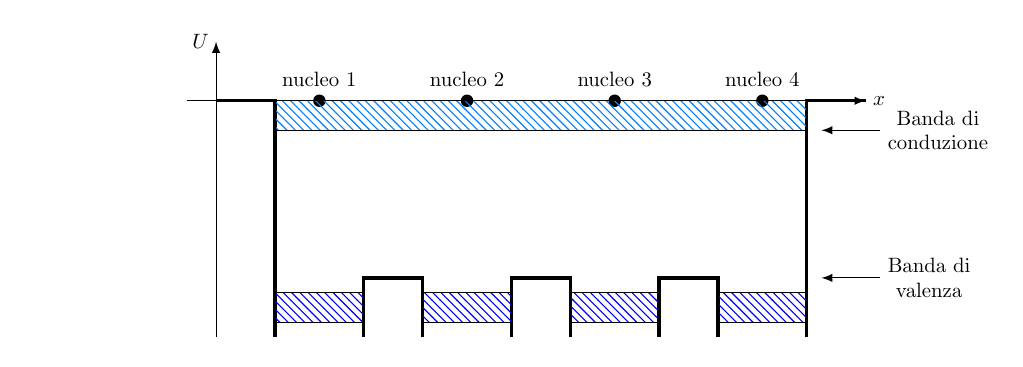
\begin{tikzpicture}[scale=0.75, transform shape]
        %disegno asse x
        \draw[-latex] (-0.5,0)-- (11,0) node[right]{$x$};
        %disegno asse y
        \draw[-latex] (0,-4)-- (0,1) node[left]{$U$};
        %disegno buche
        \draw[very thick,black] (0,0)--++ (1,0)--++ (0,-4);
        \draw[very thick,black] (2.5,-4)--++ (0,1)--++ (1,0)--++ (0,-1);
        \draw[very thick,black] (5,-4)--++ (0,1)--++ (1,0)--++ (0,-1);
        \draw[very thick,black] (7.5,-4)--++ (0,1)--++ (1,0)--++ (0,-1);
        \draw[very thick,black] (10,-4)--++ (0,4)--++ (1,0);
        %disegno i nuclei 
        \node[circle,fill=black,inner sep=0pt,minimum size=6pt,label=nucleo 1] at (1.75,0) {};
        \node[circle,fill=black,inner sep=0pt,minimum size=6pt,label=nucleo 2] at (4.25,0) {};
        \node[circle,fill=black,inner sep=0pt,minimum size=6pt,label=nucleo 3] at (6.75,0) {};
        \node[circle,fill=black,inner sep=0pt,minimum size=6pt,label=nucleo 4] at (9.25,0) {};
        %disegno bande
        \draw[pattern=north west lines, pattern color=cyan!50!blue] (1,0) rectangle (10,-0.5);
        \draw[ pattern=north west lines, pattern color=blue] (1,-3.25) rectangle (2.5,-3.75);
        \draw[ pattern=north west lines, pattern color=blue] (3.5,-3.25) rectangle (5,-3.75);
        \draw[ pattern=north west lines, pattern color=blue] (6,-3.25) rectangle (7.5,-3.75);
        \draw[ pattern=north west lines, pattern color=blue] (8.5,-3.25) rectangle (10,-3.75);
        %label bande
        \draw[latex-] (10.25,-0.5)--++ (1,0) node[align=center,right]{Banda di \\ conduzione};
        \draw[latex-] (10.25,-3)--++ (1,0) node[align=center,right]{Banda di \\ valenza};
        %per centrare la figura ricrei i label delle bande a sinistra ma li faccio invisibili
        \draw[latex-,white] (-0.25,-0.5)--++ (-1,0) node[align=center,left]{Banda di \\ conduzione};
        \draw[latex-,white] (-0.25,-3)--++ (-1,0) node[align=center,left]{Banda di \\ valenza};
    \end{tikzpicture}
    \caption{Caption}%
    \label{fig:enter_label}
\end{figure}
%
in particolare esisteranno delle bande di valenza (all'interno delle quali l'elettrone si muove con la sua massa m vera) e delle bande di conduzione.\\
%
Se introduco la massa efficace posso  vedere il sistema costituito dalle buche di potenziale periodiche in maniera semplificata come se fosse nello pazio libero, valido solo per k piccole. quello che ottengo alla fine è un qualcosa che assomiglia molto ad una sola buca di potenziale a lunghezza L ed a pareti infinite:
%
\begin{figure}[htb!]
    \centering
    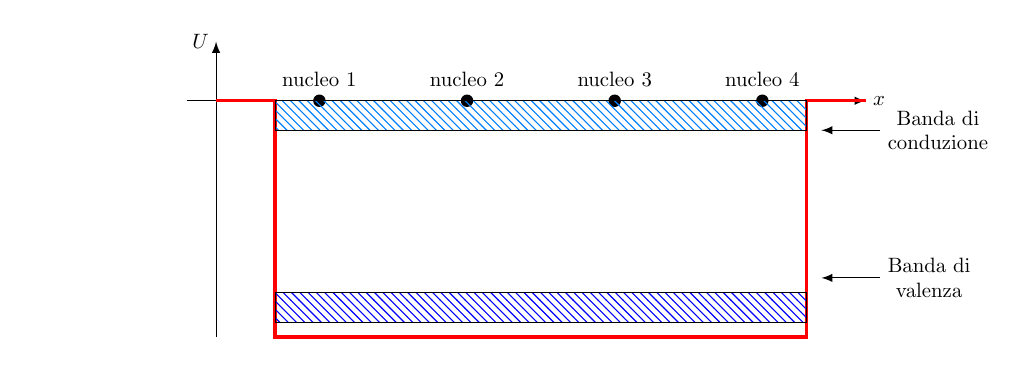
\begin{tikzpicture}[scale=0.75, transform shape]
        %disegno asse x
        \draw[-latex] (-0.5,0)-- (11,0) node[right]{$x$};
        %disegno asse y
        \draw[-latex] (0,-4)-- (0,1) node[left]{$U$};
        %disegno buche
        \draw[very thick,red] (0,0)--++ (1,0)--++ (0,-4)--++ (9,0)--++ (0,4)--++ (1,0);
        %disegno i nuclei 
        \node[circle,fill=black,inner sep=0pt,minimum size=6pt,label=nucleo 1] at (1.75,0) {};
        \node[circle,fill=black,inner sep=0pt,minimum size=6pt,label=nucleo 2] at (4.25,0) {};
        \node[circle,fill=black,inner sep=0pt,minimum size=6pt,label=nucleo 3] at (6.75,0) {};
        \node[circle,fill=black,inner sep=0pt,minimum size=6pt,label=nucleo 4] at (9.25,0) {};
        %disegno bande
        \draw[pattern=north west lines, pattern color=cyan!50!blue] (1,0) rectangle (10,-0.5);
        \draw[ pattern=north west lines, pattern color=blue] (1,-3.25) rectangle (10,-3.75);
        
        %label bande
        \draw[latex-] (10.25,-0.5)--++ (1,0) node[align=center,right]{Banda di \\ conduzione};
        \draw[latex-] (10.25,-3)--++ (1,0) node[align=center,right]{Banda di \\ valenza};
        %per centrare la figura ricrei i label delle bande a sinistra ma li faccio invisibili
        \draw[latex-,white] (-0.25,-0.5)--++ (-1,0) node[align=center,left]{Banda di \\ conduzione};
        \draw[latex-,white] (-0.25,-3)--++ (-1,0) node[align=center,left]{Banda di \\ valenza};
    \end{tikzpicture}
    \caption{Caption}%
    \label{fig:enter_label}
\end{figure}
%
gli estremi del semiconduttore rimangono invariati. La banda di valenza e conduzione che si distribuiscono in tutto il semiconduttore con elettroni che si muovono con massa efficace di opportuno valore.\\
%
Alla fine ho ottenuto un metodo che mi permette di studiare la statistica degli elettroni all'interno del semiconduttore e sono in grado di farlo perchè uso il SC come se fosse lo spazio libero $U(x) = cost$ ma, con la sola differenza che l'energia E non è continua ma rimane ancora discretizzata perchè ovviamente non siamo nel vero caso di mezzo vuoto.\\
%
\cleardoublepage%
\subsection{Densità di stati}
La densità di stati è il numero di stati disponibili per unità di volume ed energia.\\
La quantità di moto degli elettroni nel semiconduttore, approssimato come spazio libero vale:
\begin{equation}
    p=\hslash k = \sqrt{2m^*E}
\end{equation}
Ipotizzando quindi che il semiconduttore si comporti come una buca di potenziale lunga L, si avrà che i livelli energetici consentiti sono:
\begin{equation}
    E_n=\dfrac{n^2\ \hslash \ \pi^2}{2\ m^* \ L^2}
\end{equation}
Sostituendo si ha:
\begin{equation}
    p=\dfrac{n\ h}{2\ L}
\end{equation}
Ora faccio dei ragionamenti geometrici ma anche astratti:\\
Si consideri uno spazio tridimensionale, per cui la quantità di moto degli elettroni sarà composta da una combinazione di tre termini ($\overline{p}(x,y,z)$) con indice n variabile nelle tre dimensioni($ n_x, n_y, n_z$).\\
Il volume occupato da ogni stato elettronico nello spazio delle quantità di moto sarà:
%
\begin{equation}
    \left( \dfrac{h}{2L}\right)^3 \cdot \dfrac{1}{2}
\end{equation}
%
con $\left( \dfrac{h}{2L}\right)^3$ che rappresenta il volume del singolo stato e il diviso due è dovuto al fatto che lo spazio è suddiviso per le due particelle di spin opposto che possono occupare tale stato.\\
%
Il volume nello spazio delle quantità di moto ha una andamento sferico, per cui per un incremento di dp si avrà un incremento di volume di:
\begin{equation}
    \dfrac{4\pi p^2\ dp}{2^3}
\end{equation}
%
Si stanno considerando gli elettroni in banda di conduzione per cui si può riprtare la quantità di moto rispetto ad Ec:
%
\begin{equation}
    p=\sqrt{2\ m_n^* \,(E-E_c)}
\end{equation}
%
moltiplicando per dp si può trovare che
%
\begin{align}
    p\ dp & =\sqrt{2\ m_n^*(E-E_c)}\ dp \nonumber \\
    p\ dp & =\sqrt{2\ m_n^*(E-E_c)}\ d\left(\sqrt{2\ m_n^*(E-E_c)}\right) \nonumber\\
    p\,dp &= m_n^* dE
\end{align}
%
Se si realizza il rapporto tra i due volumi si trovano il numero di stati disponibili al variare di p:\\
%
\noindent\begin{minipage}{0.5\textwidth}
    %
\begin{equation}
    dN_c(p)=\dfrac{\dfrac{4\ \pi\ p^2 dp}{8}}{\left( \frac{h}{2L}\right)^3 \cdot \dfrac{1}{2}} = \dfrac{8\ \pi\ L^3\ p^2\ dp}{h^3}
\end{equation}
%
Sostituendo $pdp=m_n^*dE$ e $p=\sqrt{2\ m_n^*(E-E_c)}$ \\nell'espressione superiore e considerando $L=1$, si trova:
%
\begin{equation}
    dN_c=\dfrac{4\ \pi
    }{h^3}(2m_n^*)^{\dfrac{3}{2}}\sqrt{E-E_c} \,dE
\end{equation}
%
Analogamente si può trovare per le lacune in valenza:
%
\begin{equation}
    dN_v=\dfrac{4\ \pi
    }{h^3}(2m_h^*)^{\dfrac{3}{2}}\sqrt{E_v-E} \,dE
\end{equation}
%
\end{minipage}
\hfill%
\begin{minipage}{0.4\textwidth}\raggedleft
    \begin{center}
        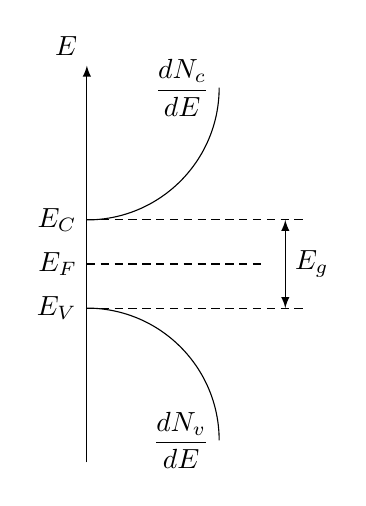
\begin{tikzpicture}[scale=0.56]
            %disegno l'asse y
            \draw[-latex] (0,-4.5) -- (0,4.5) node[anchor=south east] {$E$};
            %disegno le condentrazioni n e p
            \draw(0,1) node[left,thick]{$E_C$} arc (270:360:3) node[left]{$\dfrac{dN_c}{dE}$};
            \draw(0,-1) node[left,thick]{$E_V$} arc (90:0:3) node[left]{$\dfrac{dN_v}{dE}$};
            % tratteggi
            \draw[densely dashed] (0,1)--++ (5,0);
            \draw[densely dashed] (0,-1)--++ (5,0);
            \draw[latex-latex] (4.5,-1)--++ (0,2);
            \draw[densely dashed] (0,0) node[left]{$E_F$}--++ (4,0);
            \node at (4.5,0)[right]{$E_g$};
        \end{tikzpicture}
        \captionof{figure}{Andamento della densità di stati degli elettroni in BC e delle lacune in BV}
  \end{center}
\end{minipage}
\subsection{Distribuzione di Fermi-Dirac}
%
Tra i due livelli $E_v$ ed $E_c$ si posiziona un livello $E_F$ detto energia di fermi.\\
In generale il livello di Fermi non è noto a priori ma possiamo dire che rappresenta il livello al di sotto del quale, in condizioni di temperatura a 0 Kelvin ed in equilibrio termodinamico, tutti i livelli energetici sono occupati da elettroni mentre quelli sopra sono vuoti.\\
La densita in energia di un insieme di elettroni e lacune in equilibrio termodinamico si esprime come il prodotto di due
fattori: \textbf{la densità degli stati} (che rappresenta il numero di stati disponibili per unità di volume all'energia E) \textbf{e la funzione distribuzione} (che rappresenta la probabilita di occupazione di uno stato a energia E).\\
Anche se gli stati in un sistema quantizzato di dimensioni finite sono quantità discrete e numerabili, comunque il numero degli stati per unita di volume è cosi grande da consentire un trattamento come se fosse continuo. \\
Consideriamo il numero di stati dN di energia compresa fra
$E$ ed $E+dE$. questo é dato da: \\
%
 eq pg 64
 %
 \\
La funzione di distribuzione di Fermi-Dirac descrive la probabilità che un livello energetico E sia occupato da elettroni:
%
\begin{equation}
    f_{FD}(E)=\dfrac{1}{1+e^{\left(\dfrac{E-E_F}{k_B T}\right)}}
\end{equation}
%
Vediamo, dall'equazione, che la distribuzione di Fermi-Dirac dipende dall'energia e dalla temperatura:
Per T=0K si avrà un gradino,\textbf{indicando che tutti gli stati con energia inferiore al livello di Fermi sono pieni mentre tutti gli stati con energia superiore sono vuoti}. Per temperature seperiori si avrà un andamento esponenziale.\\
La probabilita di occupazione al livello di Fermi é pari a $\dfrac{1}{2}$ a qualsiasi temperatura. Poiché: \\
??????????????????????????
probabilita stato vuoto = 1 — probabilita stato pieno, \\
\begin{exbox}[la distribuzione di Fermi-Dirac per le lacune sara:]
    \begin{equation}
    1-f_{FD}(E)=\dfrac{1}{1+e^{\left(\dfrac{E_F-E}{k_B T}\right)}}
    \end{equation}
    In tale distribuzione complementare (a 0 K) tutti gli stati sono vuoti (di lacune)
    per energie inferiori al livello di Fermi e, tutti gli stati sono pieni per energie superiori
    al livello di Fermi.
\end{exbox} 
%
Se l'energia $E \gg E_F$, si parla di livelli energetici di conduzione. in questo caso la distribuzione di Fermi-Dirac diventa una distribuzione di Boltzman.
%
\begin{exbox}[PS: distribuzione di Boltzman]
    una distribuzione di Boltzmann (chiamata anche distribuzione di Gibbs) è una distribuzione di probabilità che fornisce la probabilità che un sistema si trovi in un determinato stato in funzione dell'energia di quello stato e della temperatura del sistema. La distribuzione è espressa nella forma:
    %
    \begin{equation}
        {\displaystyle p_{i}\propto \exp \left(-{\frac {\varepsilon_{i}}{kT}}\right)}
    \end{equation}
    %
    dove p i è la probabilità che il sistema si trovi nello stato i,$\varepsilon_i$ è l'energia di quello stato e la costante kT è il prodotto della costante di Boltzmann k e della temperatura termodinamica T .\\
    Il termine "sistema" qui ha un significato ampio; può variare da un sistema microscopico (facendo riferimento ad un singolo atomo o ad un "numero sufficiente" di atomi) a un sistema macroscopico come un serbatoio di stoccaggio del gas naturale.\\
     La distribuzione mostra che gli stati con energia più bassa avranno sempre una maggiore probabilità di essere occupati.
\end{exbox}
%
La condizione $E > E_F$ implica che l'esponenziale nella formula di $f_{FD}(E)$ sia molto più grande di 1, permettedomi di approssimare:
%
\begin{equation}
    f_{FD}(E) \approx \dfrac{1}{e^{\left(\dfrac{E-E_F}{k_B T}\right)}} = e^{\left(-\dfrac{E-E_F}{k_B T}\right)}
\end{equation}
%
Adesso sono in grado di calcolare la densità di di energia degli elettroni nella banda di conduzione n tenendo presente che il numero di elettroni dn presenti nell'intervallo da $E$ a $E+dE$ (cioé la funzione densita in energia) é pari alla densita degli stati disponibili ($dN_c$)
moltiplicata per la probabilita di occupazione $f_{FD}(E)$, cioé: 
%
\begin{equation}
    dn(E) = f_{FD}(E)\cdot dN_c
\end{equation}
%
La densita totale n si ottiene, in funzione di $E_F$, integrando $dn(E)$ su tutte le energie della banda-di-conduzione (cioé da $E_c$ all'energia del vuoto $U_0$): tuttavia-a-causa-del-comportamento esponenziale decrescente per alte energie di $f_{FD}(E)$, si può porre il limite di integrazione superiore a $+ \inf $.
\\
In parole povere, dico che n è dato dall'integrazione del prodotto tra la funzione che indica i posti disponibili e quella che indica la probabilità di occupazione.\\
%
\begin{equation}
    n=\int_{E_c}^{\inf}dN_c(E) \cdot f_{FD}(E)
\end{equation}
%
Si ottiene, nella condizione $E < E_F$ (e quindi con distribuzione di Boltzman), che la densità totale $n$ vale circa:
%
\begin{equation}
    n \approx N_c \cdot e^{\dfrac{E_F-E_C}{k_B T}}
\end{equation}
%
con $N_c=2\dfrac{{(2\pi m_n^* k_B T)}^{\dfrac{2}{3}}}{h^3} \,$ detta densità equivalente di stati in banda di conduzione.\\
$n$ rappresenta il numero di elettroni per unità di volume in banda di conduzione ed osservando la formula vedo che è dipendente dalla temperatura.\\

Il ragionamento è analogo per quanto riguarda le lacune in banda di valenza:
\begin{equation}
    p=\int_{-\inf}^{E_v}dN_v(E) \cdot [1-f_{FD}(E)]
\end{equation}
da cui 
\begin{equation}
    p \approx N_v \cdot e^{\dfrac{E_v-E_F}{k_B T}}
\end{equation}
con $N_v = 2 \dfrac{{(2\pi m_h^* k_B T)}^{\frac{2}{3}}}{h^3}$ chiamata densità equivalente di stati in banda di valenza.\\
Per le lacune la probabilità di occupazione sarà data da $1-f_{FD}(E)$ riportata sotto:
\begin{figure}[hbt!]
    \centering
    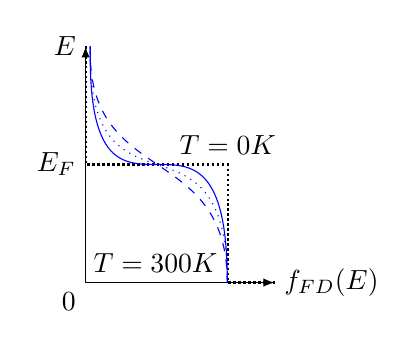
\begin{tikzpicture}[scale=0.6]
        %disegno asse x
        \draw[-latex] (0,0) node[anchor= north east]{$0$}--++ (4,0) node[right]{$f_{FD}(E)$};
        %disegno asse y
        \draw[-latex] (0,0)--++ (0,5) node[left]{$E$};;
        %disegno E
        \draw[thick, densely dotted] (0.01,5)--++ (0,-2.5) node[left]{$E_F$}--++ (3,0) node[anchor=south]{$T=0K$}--++ (0,-2.5) node[anchor=south east]{$T=300K$}--++ (1,0);
        %disegno Ffd
        \draw[blue] (0.1,5)..controls (0.01,0) and (3,5).. (3,0);
        \draw[blue,dotted] (0.1,5)..controls (0.01,1) and (3,4).. (3,0);
        \draw[blue,dashed] (0.1,5)..controls (0.01,2) and (3,3).. (3,0);
        %disegno freccia T
        
    \end{tikzpicture}
    \caption{Caption}%%
    \label{fig:enter_label}
\end{figure}
\begin{figure}[hbt!]
    \centering    
    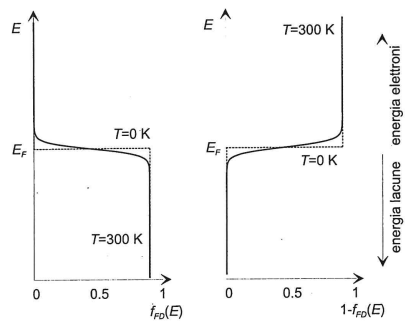
\includegraphics{Immagini_Micro&Nano/Imm_2_Fisica_dei_semiconduttori/fermi dirac.png}
    \caption{Distribuzione di Fermi-Dirac dell'energia degli elettroni e delle lacune}%
    \label{fig:Distribuzione_di_Fermi_Dirac_dell_energia_degli_elettroni_e_delle_lacune}
\end{figure}
\cleardoublepage%%
\begin{figure}
    \centering
    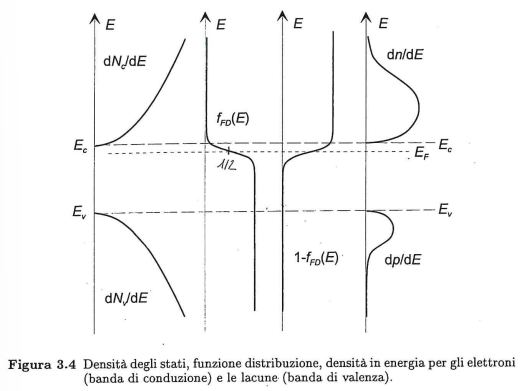
\includegraphics{Immagini_Micro&Nano/Imm_2_Fisica_dei_semiconduttori/stati, distribuzione, energia.png}
    \caption{Densità di stati, funzione di distribuzione, densità di energia per gli elettroni (nella banda di conduzione) e per le lacune (nella banda di valenza) }%
    \label{fig:Densità di stati, funzione di distribuzione, densità di energia per gli elettroni (nella banda di conduzione) e per le lacune (nella banda di valenza)}
\end{figure}
%
\cleardoublepage%%

\section*{02/10/2023}

\begin{center}
    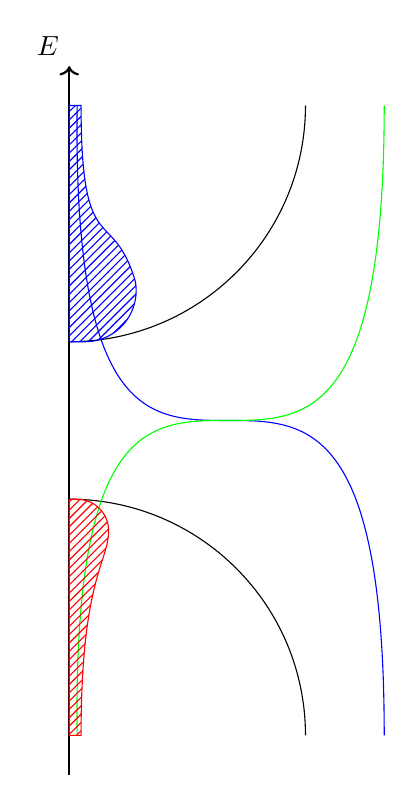
\begin{tikzpicture}    
        %disegno l'asse y
        \draw[thick,->] (0,-4.5) -- (0,4.5) node[anchor=south east] {$E$};
        %disegno le condentrazioni n e p
        \draw(0,1) arc (270:360:3);
        \draw(0,-1) arc (90:0:3);
        %disegno la densità di probabilità
        \draw[blue] (0.1,4)..controls (0,-4) and (4,4).. (4,-4);
        \draw[green] (0.1,-4)..controls (0,4) and (4,-4).. (4,4);
        %
        \draw[blue,pattern=north east lines, pattern color=blue] (0,1)-- (0.2,1) arc (270:370:0.65)..controls (0.55,2.75) and (0.15,2).. (0.15,4)-- (0,4)-- (0,1);
        %
        \draw[red,pattern=north east lines, pattern color=red] (0,-1)-- (0.1,-1) arc (90:0:0.4)..controls (0.5,-1.8) and (0.15,-2).. (0.15,-4)-- (0,-4)-- (0,-1);
    \end{tikzpicture}
\end{center}


Sulla base di queste quantità abbiamo individuato delle densità di stati 

Le abbiamo calcolate come quantità dip dall'energia e inoltre in corrispondenza del livello di fermi di arriva alla probabilità di occupaione di uno di questi stati disponibili
E sull abase del prodotto di queste due quantità, si trovava la quantità idi elettroni che in questo caso rappresenta quella dellla banda di valenza.

Nel caso specifico degli elettroni nella banda in conduzione abbiamo eq n.
Stessa cosa per lacune in banda V
Osserviamo in tutte i due i casi che l'argomento dell'esponenziale è negativo perché ef è minore del minimo della banda C ed è maggiore della banda V.
Se il live fermi per qualche motivo si spostasse verso alto o verso basso, si partirebbe da una situazione in cui le p ed n sono uguali, ad una situazione in cui (es tipo n) la funzione di distribuzione si sposta verso l'alto e quindi la distribuzione n sarà più grande e contemporaneamente una p più piccola = questo è il drogaggio N, per il tipo P succede l'opposto.

Ora dobbiamo vedere risultati che derivano direttamente da queste formule

\subsection{LEGGE DI AZIONE DI MASSA}
Sappiamo che le densità di elettroni e lacune dipendono dal livello di fermi $E_F$ tuttavia
la legge di azione di massa afferma che, in un SC non degenere ed in equilibrio
termodinamico,il prodotto $(p\cdot n)$ non dipende dalla posizione del livello di fermi.Si ha infatti:

\begin{equation}
	p \cdot n=N_C N_V \cdot \exp \left[-\dfrac{E_C-E_V}{k_B T}\right]=
        N_C N_V \cdot \exp \left[-\dfrac{E_G}{k_B T}\right]
\end{equation}

Dove $E_G$ è l'ampiezza della banda proibita del semiconduttore. \\
E' possibile osservare come pn sia inversamente proporzionale all'energy gap pertanto, materiali con $E_G$ grande presentano una minore concentrazione di elettroni in banda di conduzione ( o equivalentemente, una minore concentrazione di lacune in banda di valenza)

\textbf{Il prodotto pn quindi non dipende da $E_F$ \emph{ma solo dalla temperatura e dalle proprietà del semiconduttore}}.\\
Una diretta conseguenza di quanto detto è che il valore del prodotto pn associato ad un generico semiconduttore drogato sarà uguale al prodotto $p_i \cdot n_i$ del semiconduttore intrinseco, portando alla conclusione che il prodotto pn è indipendente dal drogaggio.
\begin{equation}
	p \cdot n=p_i \cdot n_i
\end{equation}
Dove $n_i$ e $p_i$ sono le concentrazioni nel SC intrinseco.
Poiché nel semiconduttore intrinseco elettroni e lacune si generano a coppie $(aka: p_i=n_i)$, la legge di azione di massa può essere riscritta in:
\begin{equation}
	p \cdot n=p_i \cdot n_i=p_i^2=n_i^2
\end{equation}

\begin{center}
    \begin{tikzpicture}
        \begin{axis}[
        xlabel={$\dfrac{1000}{T}$},
        ylabel={$\log(n_i^2) [cm^{-6}]$},
        axis lines=left,
        xmin=0,xmax=5,
        ymin=0,ymax=5,
        ytick={0,2,3.5,4},
        xtick={2,3,4},
        xticklabels={$3$,$4$,$5$},
        yticklabels={$10^0$, $10^8$, $10^{10}$, $10^{16}$},
        unit vector ratio=2 1.1,
        ]
            %retta nera
            \addplot [domain=0.25:3.5,samples=100,color=black,]{-0.5*x+4.1};
            \addlegendentry{$G_e$}
            %retta rossa
            \addplot [domain=0.25: 3,samples=100,color=red,]{-0.7*x+3.6};
            \addlegendentry{$S_i$}
            %retta verde
            \addplot [domain=0.65: 2,samples=100,color=green,]{-1.2*x+3};
            \addlegendentry{$G_eA_S$}
        \end{axis}

    \draw[->,blue] (4,4) node[anchor=south]{$E_G$} ..controls (3,2) and (2,1.5).. (1,1);
    
    \end{tikzpicture}
\end{center}
Riportando su grafico logaritmico la concentrazione di queste quantità in funzione dell'inverso della temperatura, succede che la concentrazione aumenta all'aumentare della temperatura e maggiore è Eg, minore sarà $ni^2$

All'aumentare della temepratura la concentraz di elett auemnta  e viceversa
Siccome gli stati hanno funzione esponenziale e siamo in grafico logaritmico, allora noi vediamo un andamento rettilineo.
L'andamento reale in realtà è approssimato, ottenuto da un'approssimazione del modello ideale.
Per T che aumenta ci sarebbero fenomeni non rettilinei 
%
\subsection{Equazioni di Shockley}
È utile in molti casi esprimere la concentrazioni di elettroni e lacune con riferimento alla concentrazione intrinseca n; e al livello di Fermi intrinseco Epi. In un
semiconduttore non degenere si ha infatti: 
%
\begin{equation}
    n=N_C \cdot \exp{\left( \dfrac{E_F-E_c}{k_B T}\right)}
\end{equation}
%
e per il semiconduttore intrinseco: 
%
\begin{equation}
    n_i=N_C \cdot \exp{\left( \dfrac{E_{Fi}-E_c}{k_B T}\right)}
\end{equation}
%
da cui, dividendo membro a membro: 
%
\begin{equation}
    n=n_i \cdot \exp{\left( \dfrac{E_{F}-E_{Fi}}{k_B T}\right)}
\end{equation}
%
Analogamente:
%
\begin{equation}
    p = p_i \cdot \exp{\left( \dfrac{E_{Fi}-E_{F}}{k_B T}\right)}
\end{equation}
%
Le relazioni precedenti, dette equazioni di Shockley, esprimono il fatto che quando
il livello di Fermi coincide con il valore intrinseco, le concentrazioni di elettroni e
lacune assumono i valori propri del materiale intrinseco $n = n_i$, $p = n_i$. Si noti
che moltiplicando le due equazioni di Shockley si ottiene $pn = n_i^2$ identicamente.
%
\subsection*{DISTRIBUZIONE DI CORRENTE}
Supponiamo di avere due semiconduttori uguali caratterizzati però da una differente posizione del livello energetico di fermi. 
\begin{center}
    \begin{tikzpicture}[scale=0.6]
        %disegno mezzo 1
        \node at (2,2) [anchor=south]{SC1};
        \draw(0,1.5) --++ (4,0);
        \draw(0,-1.5) --++ (4,0);
        \draw[dashed, red] (0,0.75) node[anchor=east]{$E_{F1}$} --++ (4,0); %Ef1
        %disegno mezzo 2
        \node at (9,2) [anchor=south]{SC2};
        \draw(7,1.5) --++ (4,0);
        \draw(7,-1.5) --++ (4,0);
        \draw[dashed, red] (7,-0.75) --++ (4,0) node[anchor=west]{$E_{F2}$}; %Ef2
    \end{tikzpicture}
\end{center}
I due semiconduttori al momento sono separati, distinti l'uno dall'altro ma cosa succede quando si uniscono?
Due o più sistemi in equilibrio termodinamico posti fra loro in contatto, sono caratterizzati dallo stesso livello di fermi. 
Tipicamente viene detto che il livello di fermi si allinea ad un certo valore costante, quindi nel nostro caso:
\begin{equation}
	E_{F1} = E_{F2}
\end{equation}

È tipo il principio dei vasi comunicanti
\newline

Perché succede questo?\\
Consideriamo due materiali semiconduttori identici caratterizzati dalla stessa densità di stati disponibili $(aka: N_{V1}=N_{V2}$ e $ N_{C1}=N_{C2})$.
L'unica cosa diversa tra i due è il livello di Fermi e, di conseguenza, anche la funzione distribuzione di probabilità di Fermi-Dirac (che per definizione è centrata intorno al livello di Fermi) sarà diversa.\\

Quindi avrò a che fare con livelli energetici occupati da elettroni nel SC1 che si affacciano a livelli energetici non occupati nel SC2.
Esisterà quindi la probabilità che una carica passi dal SC 1 al SC 2 e viceversa tuttavia, noi dobbiamo considerare il caso di equilibrio.\\
Succede che quando il sistema è in equilibrio termodinamico, la probabilità di trasferimento della carica dal mezzo 1 al 2 $(aka: P_1 \rightarrow 2)$ dovrà necessariamente essere uguale alla probabilità di trasferimento della carica dal mezzo 2 al 1 $(aka: P_{2 \rightarrow 1})$.

La probabilità $P_{1 \rightarrow 2}$ implica due condizioni:
\begin{enumerate}
    \item che lo stato di energia nel mezzo 1 sia pieno (ovvero c'è un elettrone)
    \item che lo stato di energia nel mezzo 2 sia vuoto (ovvero non ci sono elettroni)
\end{enumerate}
\begin{psbox}
    In termini detti dal libro: la probabilità di trasferimento da 1 a 2 è proporzionale al numero di stati occupati nel mezzo 1 e al numero di stati occupati nel mezzo 2.
\end{psbox}

la probabilità di passare da 1 a 2 è la probabilità congiunta di queste due osservazioni:
\begin{equation}
P_{1 \rightarrow 2} = N_{C1} (E) \cdot f_{FD1} (E) \times N_{C2} (E) \cdot \left[ 1 - f_{FD2}(E) \right] 
\end{equation}

La medesima osservazione si svolge per il passaggio da 2 ad 1:

\begin{equation}
	P_{2 \rightarrow 1} = N_{C2}(E) \cdot f_{FD2}(E) \times N_{C1}(E) \cdot  \left[ 1 - f_{FD1}(E)\right] 
\end{equation}

Dove $\left[1-f_FD (E)\right]$ indica la probabilità che il livello sia vuoto.\\
Quando queste due probabilità sono forzate ad essere identiche (perché siamo all'equilibrio e quindi si parla di trasformazione adiabatica), abbiamo che: 

\begin{equation}
	N_{C1}(E) \cdot f_{FD1}(E) \times N_{C2}(E) \cdot \left[ 1-f_{FD2}(E) \right] = N_{C2}(E) \cdot f_{FD2}(E) \times N_{C1}(E) \cdot \left[ 1-f_{FD1}(E)\right]
\end{equation}

Siccome i semiconduttori sono identici, le densità di stati saranno identiche comportandone la semplificazione dall'equazione:

\begin{equation}
	f_{FD1}(E) \times \left[1-f_{FD2}(E)\right]=f_{FD2}(E) \times \left[1-f_{FD1}(E)\right]
\end{equation}

La funzione di fermi dirac dipende unicamente dalla distanza che c'è tra il livello di energia ed il livello di fermicome mostrato dall'equazione

\begin{equation}
	f_{FD} = \dfrac{1}{1 + \exp \left[\dfrac{E-E_F}{k_B T}\right]}
\end{equation}

L'unica possibilità che abbiamo affinché l'identità sia verificata è che questi prodotti siano uno ad uno uguali fra loro:

\begin{align}
f_{FD1}(E) &= f_{FD2}(E)\\
\left[1-f_{FD2}(E)\right] &= \left[ 1-f_{FD1}(E)\right]
\end{align}


L'unica soluzione che verifica questa uguaglianza è l'allineamento del livello di Fermi per entrambi i mezzi ad un valore uguale e costante.
Nell'intorno del livello di fermi devono comunque essere rispettate le debite distanze tra le bande per cui si avrà un qualcosa come:
\begin{center}
    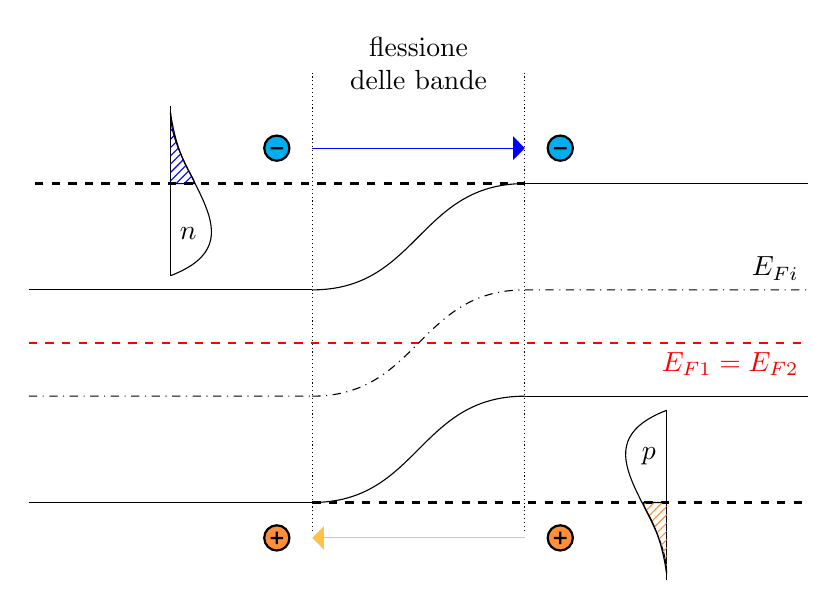
\begin{tikzpicture}[scale=0.90]
        %disegno l'unione di due SC
        %mezzo 1
        \draw(0,1.5) --++ (4,0);
        \draw(0,-1.5) --++ (4,0);
        %mezzo 2
        \draw(7,3) --++ (4,0);
        \draw(7,0) --++ (4,0);
        %livello di fermi dei mezzi
        \draw[dashed, red] (0,0.75) --++ (11,0) node[anchor=north east]
        {$E_{F1}=E_{F2}$};
        %livello di fermi del SC intrinseco
        \draw[dash dot, black] (0,0) --++ (4,0) (4,0)..controls (5.5,0) and (5.5,1.5).. (7,1.5) --++ (4,0) node[anchor=south east]
        {$E_{Fi}$};
        
        %intersezione
        \draw[] (4,1.5)..controls (5.5,1.5) and (5.5,3).. (7,3);
        \draw[] (4,-1.5)..controls (5.5,-1.5) and (5.5,0).. (7,0);
    
        %delimitazioni
        \draw[densely dotted] (4,-1.9)--++ (0,6.5);
        \draw[densely dotted] (7,-1.9)--++ (0,6.5);
        \node at (5.5,4.7) [align=center]{flessione \\ delle bande};
        \draw[thick, dashed] (4,-1.5)--++ (7,0);
        \draw[thick, dashed] (7,3)--++ (-7,0);
        %concentrazione n
        \draw(2,1.7) --++ (0,2.4);
        \draw(2,1.7)..controls (3.3,2.2) and (2,3.1).. (2,4);
        \draw[pattern=north east lines, pattern color=blue] (2,3)-- (2.34,3)..controls (2.34,3.1) and (2.1,3.3).. (2,4);
        \node at (2.25,2.3)[]{$n$};
        %concentrazione p
        \draw(9,-0.2) --++ (0,-2.4);
        \draw(9,-0.2)..controls (7.7,-0.7) and (9,-1.6).. (9,-2.5);
        \draw[pattern=north east lines, pattern color=Hcolour] (9,-1.5)-- (8.67,-1.5)..controls (8.67,-1.6) and (8.9,-1.8).. (9,-2.5);
        \node at (8.75,-0.85)[]{$p$};
        % metto elettroni
        \draw[blue, arrows={-Triangle[angle=90:6pt,blue,fill=blue]}] (4,3.5) -- (7,3.5);
        \foreach \pos in {3.5,7.5} {
        \node at (\pos,3.5) { \tikz\draw[thick, fill=Ecolour]
        circle (0.16cm) (-0.08,0)-- (0.08,0) ;} ;} 
        
        % metto lacune
        \draw[orange, arrows={-Triangle[angle=90:6pt,orange,fill=orange]}] (7,-2) -- (4,-2);
        \foreach \pos in {3.5,7.5} {
        \node at (0+\pos,-2) { \tikz\draw[thick,fill=Hcolour]
          circle (0.16cm) (-0.08,0)-- (0.08,0) (0,0.08)-- (0,-0.08) ;} ;}
    
         
    \end{tikzpicture}
\end{center}

Avrò una (flessione delle bande) che serve a definire un equilibrio tra le due.
A un certo punto la flessione crea una ???? min 48

Dal lato opposto, le lacune devono vincere la barriera di potenziale e siccome sono di segno contrario, questo corrisponde a scendere nella barriera
--------da aggiungere

-----
pg 150-168\\
Io conosco ni  del sc intrinseco ed n del drogato eq di shotkey

Mi interessa sapere come le cariche si muovono all'interno del semiconduttore.
\begin{center}
    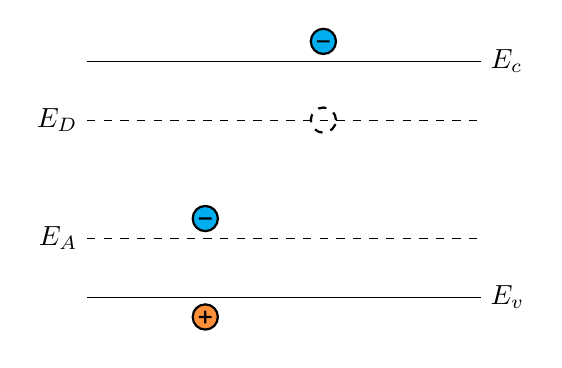
\begin{tikzpicture}
        %disegno semiconduttore
        \draw(0,0)--++ (5,0) node[right]{$E_v$};
        \draw(0,3)--++ (5,0) node[right]{$E_c$};
        %disegno livelli energetici
        \draw[dashed] (0,0.75) node[left]{$E_A$}--++ (5,0);
        \draw[dashed] (0,2.25) node[left]{$E_D$}--++ (5,0);
        %disegno elettroni
        \draw(3,3.25) [thick,fill=Ecolour]circle (0.16cm) (3-0.08,3.25)-- (3+0.08,3.25);
        \draw(3,2.25) [thick,dashed]circle (0.16cm) ;
        \draw(1.5,1) [thick,fill=Ecolour]circle (0.16cm) (1.5-0.08,1)-- (1.5+0.08,1);
        %disegno lacune
        \node at (1.5,-0.25) { \tikz\draw[thick,fill=Hcolour]
          circle (0.16cm) (-0.08,0)-- (0.08,0) (0,0.08)-- (0,-0.08) ;} ;
    \end{tikzpicture}
\end{center}

\subsection{corrente di deriva (o trascinamento) - legge di Ohm}
Devo comprendere come si muovono le cariche quando il semiconduttore è sottoposto ad un campo elettrico costante.\\
Io so che la presenza del campo $\mathcal{\vec{E}}$ genera sui portatori di carica, una forza (uguale in valore assoluto sia sugli elettroni che sulle lacune) e quindi una corrente chiamata di trascinamento.\\
%
\begin{equation}
 \vec{J}=-qn\vec{v}
\end{equation}
%
(situazione analoga per le lacune, per necessità si riassunto di ometterà spesso)\\
%
Se il reticolo fosse ideale, elettroni e lacune si muoverebbero come particelle libere, dotate di massa inerziale pari alla massa efficace, ossia di moto accellerato. Una diretta conseguenza di questa osservazione è che la velocità media dei portatori dovrebbe aumentare linearmente nel tempo ma ovviamente questo non succede.\\
Poichè il reticolo non è ideale esistono meccanismi, quali collosioni con impurità e fononi, attraverso i quali il gas di elettroni e di lacune \textbf{cede energia e quantità di moto al reticolo}, aumentando la temperatura di quest'ultimo (effetto joule).\\

Quello che mi interessa sapere è quanta parte della quantità di moto ricevuta dal campo elettrico viene ceduta al reticolo.\\
Per fare questo basta tenere presente che i meccanismi di scambio energetico e di quantità di moto quando il campo è applicato, sono gli stessi che agiscono per riportare all'equilibrio termodinamico il semiconduttore.\\

La quantità di moto di un singolo elettrone varia nel tempo per effetto della forza applicata:
%
\begin{equation}
    \dfrac{d\vec{p}}{dt}=\vec{F}=-q \mathcal{\vec{E}}
\end{equation}
%
Devo però tener conto anche dell'effetto delle collisioni sulla quantità di moto. Pertanto, si può scrivere la variazione della quantità di moto come somma di due contributi
\begin{equation}
   \dfrac{d\vec{p}}{dt} =\left. \dfrac{d\vec{p}}{dt}\right\vert_{CAMPO} + \left. \dfrac{d\vec{p}}{dt}\right\vert_{COLLISIONI} = -q \mathcal{\vec{E}} + \dfrac{p}{\tau_p}
\end{equation}
%
dove $p$ è la quantità di moto e $\tau_p$ è il tempo di vita medio o tempo di rilassamento.
Si nota subito dall'equazione che le collisioni tendono a smorzare la quantità di moto mentre il campo tende ad aumentarlo.\\
%
\begin{psbox}
    $\dfrac{p}{\tau_p}$ è il termine usato modellare il processo di decadimento della quantità di moto dovuto a collisioni o altre interazioni dissipative.\\
    Nel momento in cui $\mathcal{\vec{E}}=0$ si ha $\dfrac{d\vec{p}}{dt} \alpha  \dfrac{p}{\tau_p}$\\
    $\rightarrow$ maggiori collisioni significa maggior quantità di moto \\
    $\rightarrow$ se gli elettroni non si muovono allora non ci sono collisioni
\end{psbox}
%
In condizioni stazionarie (cioè a regime,  quindi un campo elettrico applicato da un tempo infinito), le derivate temporali si annullano. si ha quindi:
%
\begin{equation}
   \dfrac{d\vec{p}}{dt} = 0 = -q \mathcal{\vec{E}} + \dfrac{p}{\tau_p}
\end{equation}
%
Da cui:
%
\begin{equation}
   \vec{p}=-q\tau_p\mathcal{\vec{E}}
\end{equation}
%
Introducendo la velocità media, la massa efficiacie degli elettroni e sapendo che $\vec{p}=m_n^* \vec{v}$, si trova:
%
\begin{equation}
    \vec{v}=\dfrac{q\tau_p\mathcal{\vec{E}}}{m_n^*}= \mu \mathcal{\vec{E}}
\end{equation}
%
dove $\mu=\dfrac{q\tau_p}{m_n^*}$ è detto \textit{mobilità dei portatori}.\\
La mobilità dei portatori (elettroni e lacune) lega la velocità al campo elettrico:
%
\begin{equation}
    \vec{v}=- \mu \mathcal{\vec{E}}
\end{equation}
%
da cui posso ricavare l'espressione della corrente di deriva:
%
\begin{equation}
    \vec{J}=qn\mu \mathcal{\vec{E}}
\end{equation}
%
C'è però un problema: \textbf{$\mu$ non è costante !}\\
L'andamento di mupuò essere riassunto nella seguente figura:\\
%
\begin{center}
    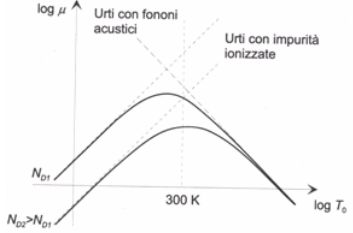
\includegraphics[scale=0.75]{Immagini_Micro&Nano/Imm_2_Fisica_dei_semiconduttori/2}
\end{center}
%
Quando al semiconduttore è applicato un campo elettrico di bassa intensità il parametro $\mu$ dipende dalle caratteristiche finisce del semiconduttore, in particolare a:
%
\begin{enumerate}
    \item urti con impurità ionizzate (ovvero al drogaggio)
    \item urti con fononi acustici (vibrazioni reticolari)
\end{enumerate}
%
I due meccanismi presentano un diverso comportamento in funzione della temperatura del reticolo.
Gli urti con impurità ionizzate hanno un tempo di rilassamento con andamento crescente rispetto alla temperatura, mentre gli urti con fononi acustici hanno un $\tau$ con andamento decrescente con la temperatura T.\\
Data quindi la presenza di due fenomeni non interagenti è possibile seguire una particolare regola che suggerisce il prevalere della mobilità $mu$ inferiore alle altre.\\
%
\begin{exbox}
    A basse temperature prevale al mobilità derivante da urti con impurità ionizzate dovute al drogaggio:
    Se faccio un drogaggio N, gli elettroni disponibili alla conduzione aumenteranno ma allora si avranno più cariche che si muoveranno poichè interagiscono con il campo elettrico dell'atomo drogante e quindi subiranno più rallentamenti e collisioni (è per questo che se N aumenta, mu diminuisce).
    A basse temperature, gli atomi del reticolo rimangono fermi, quindi gli unici a fornire contributo al numero di collisioni saranno gli elettroni mobili con gli atomi del drogaggio

\end{exbox}
%
\begin{exbox}
    A temperature elevate (intorno a 300K) prevale la mobilità derivante da urti con fononi acustici.\\
    All'aumentare di T, Il reticolo reagisce generando una vibrazione meccanica, cioè un'onda acustica che poi colpisce gli elettroni provocandone la spinta e la deviazione di traiettoria.
\end{exbox}
%
----------------
fig
\begin{center}
    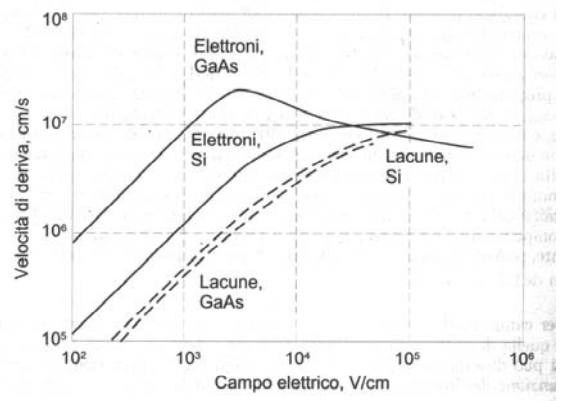
\includegraphics[scale=0.55]{Immagini_Micro&Nano/Imm_2_Fisica_dei_semiconduttori/3.png}
\end{center}

\subsection{Corrente di diffusione}

\begin{center}
    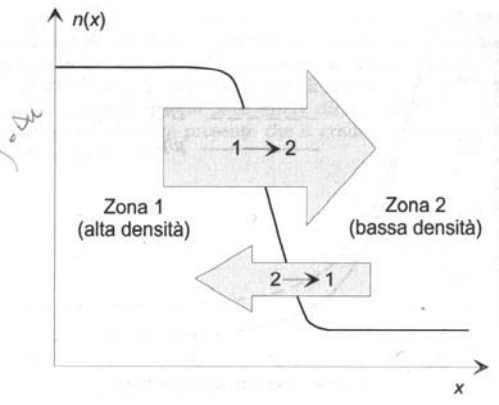
\includegraphics[scale=0.55]{Immagini_Micro&Nano/Imm_2_Fisica_dei_semiconduttori/5.png}
\end{center}
%
Poichè elettroni e lacune sono particelle cariche, pur rimanendo nell'intorno del loro punto di nascita, l'agitazione termica li fa muovere a destra e sx. A questo flusso di particelle è associato un flusso di carica e quindi una densità di corrente di diffusione:
%
\begin{align}
    \vec{J}_{n,d}&=qD_n\nabla_n\\
    \vec{J}_{h,d}&=-qD_h\nabla_p
\end{align}
%
dove $D_n$ è la diffusività degli elettroni e $D_p$ è la diffusività delle lacune.\\
L'equazione precedente sta  a dire che il gradiente di concentrazione produce una velocità media di diffusione del gasi di lacune ed elettroni pari a 
\begin{align}
    \vec{v}_{n,d}=-D_n \dfrac{\nabla n}{n}\\
    \vec{v}_{h,d}=-D_h \dfrac{\nabla p}{p}
\end{align}

la corrente misurabile totale è quindi la somma della corrente di deriva e di diffusione:

\begin{equation}
    \vec{J}_n^{TOT}=-qn\mu\mathcal{\vec{E}} + qD_n\nabla n
\end{equation}

\begin{psbox}
    se prendo un semiconduttore non connesso ad una batteria ($\vec{J}_n^{TOT}=0$) ma con un certo gradiente di concentrazione ($\nabla n \neq 0$), allora all'interno del semiconduttore si creerà un campo elettrico $\mathcal{\vec{E}}$ che bilancia la corrente di deriva e di diffusione in modo da soddisfare $\vec{J}_n^{TOT}=0$
\end{psbox}


\subsection{la relazione di Einstein}
La relazione di Einstein vale solo per semiconduttori non degeneri ed afferma che,\textit{in condizioni di equilibrio termodinamico e di basso campo $\mathcal{E}$, diffusività e mobilità sono proporzionali}. Questo è descritto dall'equazione di Einstein:
%
\begin{equation}
    D_n=\dfrac{k_B T_0}{q}\mu_{n0}
\end{equation}
%
\begin{equation}
    D_h=\dfrac{k_B T_0}{q}\mu_{h0}
\end{equation}
%
In condizioni di alto campo la diffusività si
discosta dalla relazione di Einstein; Mentre la mobilità tende a zero (infatti la velocità dei portatori satura) la diffusività tende ad un valore costante,
inferiore al valore di basso campo. 
%
\begin{figure}[hbt!]
    \centering
    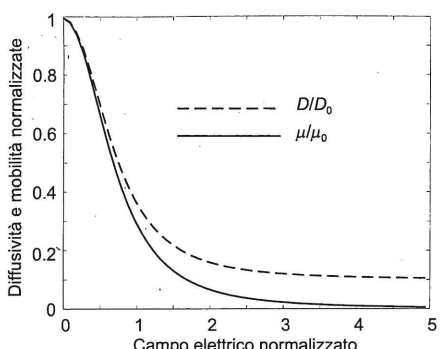
\includegraphics{Immagini_Micro&Nano/Imm_2_Fisica_dei_semiconduttori/grafico relazione di einstein.png}
    \caption{Caption}%
    \label{fig:enter_label}
\end{figure}
%
\cleardoublepage%

\section*{05/10/2023}
\section{Semiconduttori soggetti a perturbazione esterna}
Voglio studiare i diversi casi di semiconduttore soggetto a perturbazione esterna.
Prendo due equazioni. La prima è la densità di corrente di elettroni totale:
\begin{equation*}
    \vec{J}_n^{tot}=-qn \mu_n \mathcal{\vec{E}}+qD_n \dfrac{dn}{dx}
\end{equation*}

Dove, dalla equazione di Einstein abbiamo ricavato che
\begin{equation*}
    \mu_n=\dfrac{D_n}{V_T}
\end{equation*}
con
$V_T= \dfrac{k_B T}{q}\approx 25mV$\\
La seconda equazione necessaria per proseguire è chiamata "equazione di continuità" di elettroni e lacune:\\
Si consideri un insieme di cariche mobili in un mezzo materiale. Si supponga, in un primo momento, che le cariche mobili in gioco siano soggette solo al trasporto.
Siano allora Q la carica in un volume V, limitato da una superficie $\Sigma$ dotata di versore normale n diretto verso l'esterno, J la densità di corrente. La conservazione della carica totale Q implica:
\begin{equation}
    \dfrac{dQ}{dt}+\nabla J =0
\end{equation}

In realtà nel caso più generale devo considerare che le cariche in gioco siano soggette non solo al trasporto ma anche alla generazione-ricombinazione.
Pertanto, l'equazione di continuità deve essere arricchita con il terzo termine $U_Q$ chiamato tasso di ricombinazione/generazione. Questo parametro definisce la quantità di carica che scompare nell'unità di tempo per effetto della ricombinazione.
La conservazione della carica totale Q generale è:
\begin{equation}
     \dfrac{dQ}{dt}+\nabla J +U_Q=0
\end{equation}
L'equazione di continuità della carica può pertanto esprimersi come:
variazione temporale della carica volumica + divergenza della densità di corrente + tasso netto volumico di ricombinazione della carica = 0

\subsection{Tasso di Ricombinazione}
Questo Uq termine è legato a diversi fattori:
*) assorbimento di fotoni
*)collisione
*)trappole o difetti\\
L'equazione di ricombinazione e generazione$U_Q$ è meglio definita come segue:
\begin{equation*}
    U_Q=+G-R
\end{equation*}
Più precisamente si indicheranno i termini con pedice "n" nel caso di generazione e ricombinazione di elettroni e con pedice "h" nel caso di generazione e ricombinazione di lacune.\\
Parlando di elettroni:
\begin{equation*}
    U_{Qn}=G_n-R_n
\end{equation*}
La variazione di concentrazione di cariche in eccesso al variare del tempo è definito come:
\begin{equation*}
    \dfrac{dn'}{dt}=G_n-R_n
\end{equation*}
In caso di semiconduttore in condizione stazionaria la concentrazione di elettroni in eccesso è nullo, pertando generazione e ricombinazione si equivalgono.
\begin{equation*}
    0=G_n - R_n
\end{equation*}
Tuttavia, a causa di diversi motivi (quali sorgente luminose) può accadere ad un certo punto che ci sia elevata concentrazione di carica in eccesso. Allora accade che il tasso di ricombinazione è notevolmente maggiore della generazione ($G_n \gg R_n$) e quindi posso approssimare l'equazione in quella che si userà in seguito:
\begin{equation*}
    U_{Qn}=\dfrac{dn'}{dt}=-R_n
\end{equation*}
Ora rimane da trovare il valore di $R_n$:
\begin{equation*}
    R=\dfrac{n'}{\tau_n}
\end{equation*}
da cui
\begin{equation}
    \dfrac{dn'}{dt}=-\dfrac{n'}{\tau_n}
\end{equation}
%
Dove $\tau_n$ è il tempo di vita medio degli elettroni.\\
L'equazione, riporta il segno "-" ad indicare la diminuzione della densità di portatori di carica liberi nel tempo a causa della ricombinazione.\\
Con il passare del tempo il sistema si avvicina a uno stato stazionario ritornando, ancora una volta, alla condizione $G=R$.\\




%\cleardoublepage%

\subsection{Decadimento della concentrazione in eccesso dei portatori}

Considero un normale semiconduttore non drogato (intrinseco) di lunghezza W idealmente infinita. So che la concentrazione di cariche è uniforme lungo tutto il mezzo e di valore $n_i^2$.\\
E' interessante studiare i casi che provocano la variazione della concentrazione 
\begin{center}
    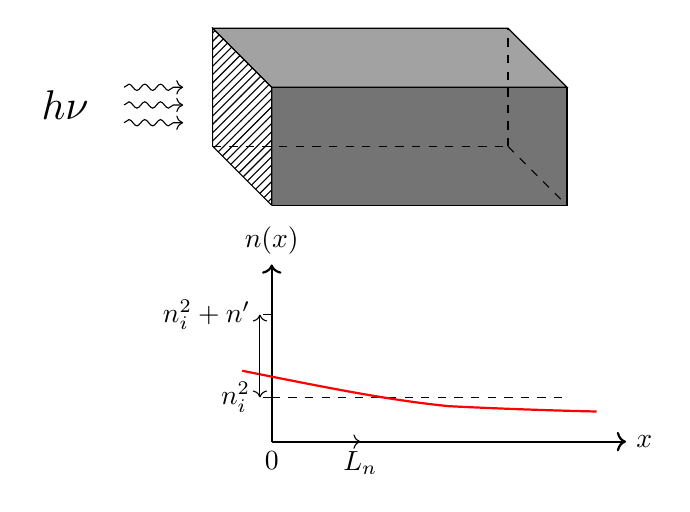
\begin{tikzpicture}[scale=0.75]
        \draw[fill={rgb:black,6;white,5}] (0,0)-- (5,0)-- (5,2)-- (0,2)-- (0,0);
        \draw[fill={rgb:black,4;white,7}] (0,2)-- (5,2)-- (4,3)-- (-1,3)-- (0,2);
        \draw[pattern=north east lines, pattern color=black] (0,0)-- (0,2)-- (-1,3)-- (-1,1)-- (0,0);       
        \draw[dashed] (-1,1)-- (4,1);
        \draw[dashed] (4,1)-- (4,3);
        \draw[dashed] (4,1)-- (5,0);

        %disegno radiazioni luminosa
        \draw[->,decorate,decoration={snake,amplitude=.4mm,segment length=2mm,post length=1mm}] (-2.5,2) --++ (1,0);
        \draw[->,decorate,decoration={snake,amplitude=.4mm,segment length=2mm,post length=1mm}] (-2.5,1.7) --++ (1,0);
        \draw[->,decorate,decoration={snake,amplitude=.4mm,segment length=2mm,post length=1mm}] (-2.5,1.4) --++ (1,0);

        %label energia fotoni
        \node at (-3.5,1.7) [scale=1.5]{$h \nu$};

        %disegno asse x
        \draw[thick,->] (0,-4) node[anchor=north]{$0$}--++ (6,0)
        node[anchor=west]{$x$};
        %disegno asse y
        \draw[thick,->] (0,-4)--++ (0,3) node[anchor=south]{$n(x)$};
        %disegno i grafici
        \draw[dashed] (0,-3.25) --++ (5,0);
        %\draw[ domain=0:5, color=red, thick, ->, samples=500] plot (\x, {exp(-\x + 0.3)} - 3.2);
        \draw[thick, red] (-0.5, -2.8) .. controls (1, -3.1) and (2, -3.3) .. (3, -3.4) .. controls (4, -3.45) and (5, -3.48) .. (5.5, -3.49);

        %label e doppia freccia
        \draw[dashed] (0,-1.85) --++ (-0.2,0) node[anchor=east]{$n_i^2+n'$};
        \draw[dashed] (0,-3.25) --++ (-0.2,0) node[anchor=east]{$n_i^2$};
        \draw[<->] (-0.2,-1.85) -- (-0.2,-3.25);
        \draw[->] (0,-4.0) -- ++ (1.5,0) node[anchor=north]{$L_n$};
    \end{tikzpicture}
\end{center}
\subsubsection*{1°Caso) Semiconduttore non drogato esposto a sorgente luminosa}
Considero un semiconduttore illuminato da una sorgente di fotoni sulla faccia posta in x=0 inoltre:
\begin{itemize}
    \item Assumo di avere fotoni ad alta energia in modo da garantire il passaggio degli elettroni dalla banda di valenza alla banda di conduzione, quando assorbono tale energia;
    %
    \item il campione è mantenuto in condizioni di circuito aperto (senza generatore collegato), ossia la corrente che fluisce nel campione è nulla in ogni sezione;
\end{itemize}
%
La pioggia di fotoni provoca una generazione superficiale di portatori in eccesso pari a $n'$ in $x=0$; questo eccesso di elettroni si smaltisce all'aumentare di x fino a quando, per $x=+\infty$, la perturbazione generata dai fotoni si è completamente annullata ($n'=0$).\\

Faccio un'ulteriore semplificazione considerando due ipotesi:\\
\begin{itemize}
    \item [\textbf{Hp.1}] il sistema è in condizioni stazionarie\\
        Questo significa che non ci sono variazioni di carica nel tempo $(\dfrac{dQ}{dt}=0)$\\
    \item [\textbf{Hp.2}] Il campo elettrico esterno è nullo $\mathcal{\vec{E}}=0$\\
        Questo implica che la corrente di deriva (detta di trascinamento) diventi, in prima approssimazione, trascurabile
\end{itemize}
Unendo l'equazione  $J_n^{tot}$ all'equazione di continuità e usando le precedenti ipotesi ottengo il seguente sistema:
%
\begin{alignat*}{4}[left = \empheqlbrace]
   0 + \dfrac{d\vec{J}^{\text{tot}}}{dx} - R_n = 0  \\
    \vec{J}^{\text{tot}}= q\,D_n \cdot \frac{dn'}{dx}
\end{alignat*}
%
La forma a cui si giunge è una EDO omogenea:
%
\begin{equation}
    D_n \cdot \dfrac{d^2 n'}{dx^2}= \dfrac{n'}{\tau_n}
\end{equation}
%
\begin{ripasso}[come risolvere l'EDO:]
La soluzione generale della EDO è:
\begin{equation*}
    n'(x)=A\cdot \exp \left( \dfrac{x}{L_n}\right) + B \cdot \exp \left( \dfrac{-x}{L_n} \right)
\end{equation*}

Le costanti A e B possono essere determinate imponendo le condizioni al contorno:
\begin{align*}
    n'(0)&=n_i^2+n' \\
    n'(\infty)&=n_i^2
\end{align*}

Pertanto
\begin{align*}
    n'(0)&=A+B=n_i^2+n'\\
    n'(\infty)&=A\cdot \infty+B=n_i^2
\end{align*}

Dall'ultima equazione si evince che $A=\dfrac{n_i^2-B}{\infty}=0$ ; mentre dalla prima si ottiene che $B=n'(0)$.\\
\end{ripasso}
%
Allora il risultato finale è l'equazione di diffusione dei portatori minoritari risulta:
\begin{equation}
    n'(x)=n'(0) \cdot \exp \left( \dfrac{-x}{L_n}\right)
\end{equation}

Dove $L_n=\sqrt{D_n \tau_n}$ è detta lunghezza di diffusione degli elettroni.\\
Quindi si osserva che, in presenza di iniezione laterale di portatori in eccesso, \textbf{le concentrazioni di eccesso tendono ad annullarsi con legge esponenziale decrescente} con una lunghezza tipica $L_n$  tanto maggiore quanto più lungo il tempo medio dei portatori in eccesso.\\
La corrente di diffusione vale:
%
\begin{equation}
    J_{n,d}(x)=qD_n \dfrac{dn'(x)}{dx}=qD_n \dfrac{d}{dx}\left( n'(0) e^{\dfrac{-x}{L_n}}\right)=-q\sqrt{\dfrac{D_n}{\tau_n}}(n_i^2+n')\exp(-x/L_n)
\end{equation}
%
La corrente di lacune corrispondente tale da soddisfare la condizione di quasi neutralità si scrive:
%
\begin{equation}
    J_{h,d}(x)=-qD_h \dfrac{dp'(x)}{dx}=\dfrac{qD_h}{L_h}(n_i^2+n')\exp(-x/L_h)=q\sqrt{\dfrac{D_h}{\tau_h}}(n_i^2+n')\exp(-x/L_h)
\end{equation}
%
E' quindi importante notare che se le due correnti sono uguali e contrarie, allora i tempi di vita media e la diffusività di elettroni e lacune sono uguali. in questo caso la corrente totale è nulla ed è quindi rispettata la condizione di circuito aperto alla parete sinistra del semiconduttore. \\
%
\textbf{Se questo non accadesse, significherebbe che le due correnti di diffusione sono differenti e si stabilirebbe quindi una condizione di non neutralità che a sua volta genera un campo elettrico tale da provocare una corrente di deriva che renda nulla la corrente totale}.

Mi interessa analizzare il comportamento di un semiconduttore in presenza di uno scostamento dalla neutralità nel tempo e nello spazio.\\
Per permettere una semplice analisi quantitativa si suppone che lo scostamento sia piccolo, ossia che il semiconduttore operi in condizioni di piccolo segnale.\\
Consideriamo due casi di scostamento della neutralità:
%
\begin{enumerate}
    \item scostamento dalla neutralità uniforme nello spazio ma dipendente dal tempo (tempo-variante);
    \item scostamento dalla neutralità uniforme nel tempo ma dipendente dallo spazio.
\end{enumerate}
%
Per entrambi i casi si considera un semiconduttore drogato di tipo n e monodimensionale (direzione solo lungo le x, per semplificare le operazioni di derivazione)\\

\paragraph{Scostamento dalla neutralità nel tempo}\mbox{}\\
Se ho un semiconduttore drogato con una concentrazione di atomi donori pari ad $N_D$ (ed uno di questi dona 1 elettrone), la concentrazione di elettroni nel tempo sarà circa il numero di atomi donori più i portatori in eccesso:
%
\begin{align}
    n(t)&=n_0+n'(t)\approx N_D+n'(t)
\end{align}
%
\begin{align*}
    (n'&\ll n_0 )
\end{align*}
%
Dove la concentrazione degli elettroni $n_0$ è assunta uguale alla concentrazione di atomi donori $N_D$, mentre $n'(t)$ rappresenta l'eccesso locale di elettroni sul SC drogato nel caso, di un altro SC maggiormente drogato posto a contatto.\\
La concentrazione delle lacune rimane invariata:
%
\begin{align}
    p(t)&=p_0
\end{align}
%
\begin{align*}
    (p_0&\ll n_0)
\end{align*}
%
\begin{psbox}[ATTENZIONE]
 $p(t)=p_0 \neq p_i$
Infatti, per la legge di azione di massa, in un generico semiconduttore: $n\cdot p=n_i \cdot p_i$ ;
quindi se $n\uparrow$, necessariamente $p\downarrow$ in modo da mantenere soddisfatta l'equivalenza.
Pertanto, nel caso di semiconduttore drogato n si avrà che:
il numero di elettroni aumenta ($n=n_0=N_D$ )e il numero di lacune diminuisce ($p=p_0 $)
\end{psbox}
%
L'eccesso locale di elettroni causa una variazione del campo elettrico e quindi del potenziale $\phi(t)$:
%
\begin{equation}
    \phi(t)=\phi_0+\phi'(t)
\end{equation}
Ricordo che sto studiando il caso semplice di semiconduttore omogeneo (per cui la variazione di $n$ è indipendente nello spazio: $\dfrac{dn}{dx}=0$) ovvero sto trascurando la corrente diffusiva, allora la densità di corrente di elettroni vale: 
%
\begin{equation}
    J_n=-qn \mu_n \dfrac{d\phi}{dx}
\end{equation}
%
Adesso inserisco $J_n$ nell'equazione di continuità trascurando l'effetto della ricombinazione-generazione (poiché ci sono talmente tante cariche che$ \dfrac{n'}{\tau}\rightarrow 0$), ottenendo:
%
\begin{align}
    q \dfrac{dn}{dt} &+\nabla \cdot J_n=0\\
    q \left[ \dfrac{dN_D}{dt} + \dfrac{dn'(t)}{dt}\right] &+ \nabla \cdot \left[ -qn\mu_n \dfrac{d\phi}{dx} \right] = 0 \nonumber\\
    q \left[ 0 + \dfrac{dn'(t)}{dt}\right] &+ \nabla \cdot \left[ -qn\mu_n \dfrac{d\phi}{dx} \right] = 0 \nonumber\\
    q \dfrac{dn'(t)}{dt} &= qn \mu_n \left[ \nabla \cdot \dfrac{d\phi}{dx} \right] \nonumber
\end{align}
%
In conclusione 
%
\begin{equation}
    \dfrac{n'(t)}{dt}=\mu_n n \dfrac{d^2 \phi}{dx^2}
\end{equation}
%
Questa equazione assomiglia molto ad una EDO, peccato la presenza di due variabili sotto le derivate.
Tuttavia, in questa equazione posso applicare una semplificazione considerando che all'interno cé la cosiddetta equazione di Poisson:
%
\begin{equation}
    \dfrac{d^2 \phi}{dx^2} = \dfrac{q}{\epsilon}n'(t)
\end{equation}
%
Pertanto, l'eccesso nel tempo avrà forma:
%
\begin{equation}
    n'(t)=n'(0)+\exp \left[ \frac{-t}{\tau_D} \right]
\end{equation}
%
Dove $\tau_D= \dfrac{\epsilon}{qN_d \mu_n}= \dfrac{\epsilon}{\sigma_n}$ è detto tempo di
rilassamento dielettrico. Il parametro $\sigma_n$ è la conducibilità elettrica del
semiconduttore dovuta ai soli elettroni, che equivale in questo caso alla 
conducibilità totale.\\
%
\begin{psbox}[NOTA]
Dall'equazione precedente si nota che 
$\tau_D$  $1/\alpha$  $ \mu$, $ N_D$\\
Pertanto, aumentare la concentrazione di atomi donori oppure la mobilità dei portatori, significa anche aumentare la velocità di ritorno alla condizioni di equilibrio che corrisponde ad avere un dispositivo che risponde (o commuta) più velocemente.\\
Ogni materiale ha un suo tempo di rilassamento \\
FIGURE SBAGLIATE MA BELLE.\\
e nel caso limite si ha il pec, un metallo caratterizzato da $\tau_D \approx 0$:
Quando $V_{bias}$ smette di variare, gli elettroni in eccesso verranno riassorbiti nel tempo $\tau_D$, in questo caso sarà pressochè istantaneo.
%
\noindent\begin{minipage}{0.49\textwidth}
    \begin{center}
    \begin{circuitikz}
    \draw(-0.5,0) to [american voltage source, v=$V_{bias}$,invert] (0,0)--++ (0.5,0);
        \draw[pattern= north east lines] (0.5,0.5) rectangle (1,-0.5);
        \draw(1,0.5) rectangle (3,-0.5);
        \draw(3,0)--++ (0.5,0) to (3.5,-0.5) node[tlground]{};
        %disegno asse x
        \draw[thick,->] (1,-0.7) node[anchor=north]{$0$}--++ (2,0)
        node[anchor=north ]{$x$};
        %disegno asse y
        \draw[thick,->] (1,-0.7)--++ (0,2) node[anchor=south]{$n'(x)$};
        %disegno i grafici
        %\draw[smooth, domain=0:4, color=red, thick] plot (\x, {exp(-\x + 0.3) - 1});

    \end{circuitikz}
\end{center}
\captionof{figure}{CaptionA}
\end{minipage}
\hfill%
\begin{minipage}{0.49\textwidth}\raggedleft
    \begin{center}
    \begin{circuitikz}
    \draw(-0.5,0) to [american voltage source, v=$V_{bias}$,invert] (0,0)--++ (0.5,0);
        \draw[pattern= north east lines] (0.5,0.5) rectangle (1,-0.5);
        \draw(1,0.5) rectangle (3,-0.5);
        \draw(3,0)--++ (0.5,0) to (3.5,-0.5) node[tlground]{};
        %disegno asse x
        \draw[thick,->] (1,-0.7) node[anchor=north]{$0$}--++ (2,0)
        node[anchor=north ]{$x$};
        %disegno asse y
        \draw[thick,->] (1,-0.7)--++ (0,2) node[anchor=south]{$n'(x)$};
        %disegno i grafici
        %\draw[smooth, domain=0:4, color=red, thick,scale=0.5] plot (\x+2,{\exp((-\x+0.3)) -1});
    \end{circuitikz}
\end{center}
\captionof{figure}{Caption B}
\end{minipage}
%
\end{psbox}
%
\cleardoublepage%

\paragraph{Scostamento dalla neutralità nello spazio}
Per uno scostamento dalla neutralità costante nel tempo ma funzione dello spazio si può scrivere:

\begin{align}
    n(x)&=n_0+n'(x)\approx N_D+n'(x)
\end{align}
\begin{align*}
    (n'&\ll n_0 )
\end{align*}
Dove la concentrazione degli elettroni $n_0$ è assunta (anche giustamente) uguale alla concentrazione di atomi donori $N_D$.
Dove $n'(x)$ rappresenta l'eccesso locale di elettroni sul SC drogato nel caso, per esempio, di un altro SC maggiormente drogato posto a contatto.
La concentrazione delle lacune rimane invariata:
\begin{align}
    p(x)&=p_0
\end{align}
\begin{align*}
    (p_0&\ll n_0)
\end{align*}

PS: su $p(x)$ vale l'osservazione del caso precedente.

L'eccesso locale di elettroni nello spazio causa una variazione di potenziale $\phi(x)$:
\begin{equation}
    \phi(x)=\phi_0+\phi'(x)
\end{equation}
Si va a considerare J (questa volta ci sarà una corrente diffusiva a causa della variazione di concentrazione di elettroni dello spazio):

\begin{equation}
    J_n=-q \mu_n n \dfrac{d\phi}{dx}+qD_n \frac{dn}{dx}
\end{equation}

e lo si inserisce nell'equazione di continuità trascurando l'effetto della ricombinazione-generazione (poiché ci sono talmente tante cariche che $ \dfrac{n'}{\tau}\rightarrow 0$) e trascurando la variazione di carica nel tempo (poiché stiamo considerando il caso di neutralità costante nel tempo: $\dfrac{dQ}{dt}=0$):
\begin{align}
    \nabla J_n=0
\end{align}
Risolvendo:
\begin{align}
    \nabla \cdot \left[ q \mu_n n \dfrac{d \phi}{dx} + q D_n \dfrac{dn}{dx}\right] &=0 \nonumber\\
    -q \mu_n n \nabla \cdot \dfrac{d\phi}{dx}       + qD_n \nabla \cdot \frac{dn}{dx}&=0 \nonumber\\
    qD_n \nabla \cdot \left[ \frac{dN_D}{dx} + \dfrac{dn'(x)}{dx} \right] &= q \mu_n n \nabla \cdot
    \dfrac{d\phi}{dx} \nonumber\\
    qD_n \nabla \cdot \left[ \frac{dN_D}{dx} + \dfrac{dn'(x)}{dx} \right] &= q \mu_n n \nabla \cdot 
    \dfrac{d\phi}{dx} \nonumber
\end{align}
In conclusione, 
\begin{equation}
    D_n \dfrac{d^2 n'(x)}{dx^2}= \mu_n n \dfrac{d^2\phi}{dx^2}
\end{equation}

Questa equazione assomiglia molto ad una EDO, peccato che non posso risolverla così com'è perchè ci siano due variabili diverse sotto derivata
Tuttavia, in questa equazione posso applicare una semplificazione considerando che all'interno cé la cosiddetta equazione di Poisson: 
\begin{equation}
    \dfrac{d^2 \phi}{dx^2} = \dfrac{q}{\varepsilon}n'(t)
\end{equation}

Pertanto, l'eccesso nel tempo avrà forma:
\begin{equation}
    n'(t)=n'(0)+\exp \left[ \frac{-x}{L_D} \right]
\end{equation}

Dove $L_D=\sqrt{\dfrac{\varepsilon k_B T_0}{q^2 N_D}}$ è detta lunghezza di Debye. \\
\begin{exbox}[Un pò di numeri]
Nel silicio a temperatura ambiente:
\begin{align*}
    N_D&=10^{-16} && \,cm^{-3}\\
    \mu_n&=10^{3} && \,cm^{2}/s\\
    L_D&=10^{-8}  && \,m\\
    \tau_D&=10^{-13} && \,s
\end{align*}
    Proff figura?
\end{exbox}

Quindi che le perturbazioni locali o temporali dalla neutralità tendono  a smorzarsi con tempo dell'ordine del tempo di rilassamento dielettrico i in lunghezze dell'ordine della lunghezza di Debye, quando non vengano mantenute da cause esterne(caso giunzione polarizzata).\\

Con questi strumenti sono in grado di studiare bene come operano tre tipi di giunzione molto importanti:
\begin{enumerate}
    \item giunzione tra due semiconduttori uguali ma con drogaggio diverso (giunzione PN) $(E_{g1} =E_{g2})$
    \item giunzione tra metallo e semiconduttore $(E_{g,metal} =0 ; E_{g1})$
    \item giunzione tra due semiconduttori completamente diversi tra solo $(E_{g1} \neq E_{g2} )$
\end{enumerate}
\cleardoublepage%

\noindent\begin{minipage}{0.9\textwidth}
    \section{giunzione tra due semiconduttori uguali ma con drogaggio diverso, il diodo P-N}
\end{minipage}
\begin{minipage}{0.1\textwidth}\raggedleft
    \begin{pgGhione}
    255
    \end{pgGhione}
\end{minipage}

\subsection{studio qualitativo}
figura
il semiconduttore N ha un livello di fermi più alto, rendendo più semplice il passaggio degli elettroni dalla banda di valenza alla banda di conduzione, e viceversa.\\
Nel caso in cui due semiconduttori con livelli di energetici diversi vengano messi a contatto, i livelli energetici di fermi si stabilizzano ad un valore costante:
Ma se il livello di fermi deve rimanere costante, tutto il resto dovrà cambiare\\
\begin{figure}[hbt!]
    \centering
    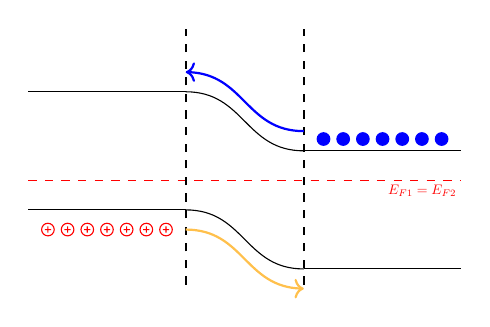
\begin{tikzpicture}[scale=0.5,transform shape]
        %disegno l'unione di due SC
        %mezzo 1
        \draw(0,3) --++ (4,0);
        \draw(0,0) --++ (4,0);
        %mezzo 2
        \draw(7,1.5) --++ (4,0);
        \draw(7,-1.5) --++ (4,0);
        %livello di fermi
        \draw[dashed, red] (0,0.75) --++ (11,0) node[anchor=north east]{$E_{F1}=E_{F2}$};
        %intersezione
        \draw[] (4,3)..controls (5.5,3) and (5.5,1.5).. (7,1.5);
        \draw[] (4,0)..controls (5.5,0) and (5.5,-1.5).. (7,-1.5);
        %lacune
        \foreach \pos in {0.5,1,1.5,2,2.5,3,3.5} {
        \node at (0+\pos,-0.5) { \tikz\draw[thick,red]
          circle (0.16cm) (-0.08,0)-- (0.08,0) (0,0.08)-- (0,-0.08) ;} ;}
        %elettroni
          \foreach \pos in {0.5,1,1.5,2,2.5,3,3.5} {
        \node at (7+\pos,+1.8) { \tikz\draw[thick,blue, fill=blue]
          circle (0.16cm)  ;} ;}
        %delimitazioni
        \draw[thick, dashed] (4,-1.9)--++ (0,6.5);
        \draw[thick, dashed] (7,-1.9)--++ (0,6.5);
        %altro
        \draw[blue,thick,<-]
        (4,3.5)..controls (5.5,3.5) and (5.5,2).. (7,2);
        \draw[orange,thick,->]
        (4,-0.5)..controls (5.5,-0.5) and (5.5,-2).. (7,-2);
    \end{tikzpicture}
    \caption{Caption}%
    \label{fig:enter_label}
\end{figure}
Figura e spiegazione\\
Ricavo che dalla zona P si avrà un eccesso di lacune, una piccolissima quantità di elettroni liberi ed una grandissima quantità di ioni negativi denominate cariche stazionarie (o ioni accettori fissi). Trascurando l'effetto di questi pochi elettroni liberi, posso dire che le lacune sono bilanciate dalle cariche stazionare negative per rendere la zona elettricamente neutra.\\
Il ragionamento è duale per quanto riguarda la regione drogata tipo N (con gli equivalenti ioni donori fissi) .\\

%
\noindent\begin{minipage}{0.55\textwidth}
Nel memento in cui questi due mezzi sono posti a contatto, a cavallo della giunzione si presenta una differenza di concentrazione delle lacune fra zona P e zona N, rappresentate rispettivamente con Na ed Nd.
Questo gradiente produce una diffusione di lacune che dalla zona drogata P si diffondono verso quella drogata N.\\
le stesse considerazioni valgono per gli elettroni liberi in zona N.\\
Questo fenomeno di diffusione presenta importanti conseguenze;
ricordo che le due zone sono elettricamente neutre, cioè per ogni elettrone (lacuna) nella zona N (P) ci sarà uno ione fisso positivo (ione fisso negativo).
Appena il primo elettrone libero si sposta dalla zona N ed arriva in zona P, trasportando con sé la propria carica elettrica, esso produce un'alterazione della neutralità di carica: la zona P si ritrova con una carica negativa in più, mentre la zona N se ne ritrova una in meno.
Ciò crea a cavallo della giunzione, un campo elettrico diretto verso P.\\
\end{minipage}
\hfill%
\begin{minipage}{0.4\textwidth}\raggedleft
    \begin{center}
    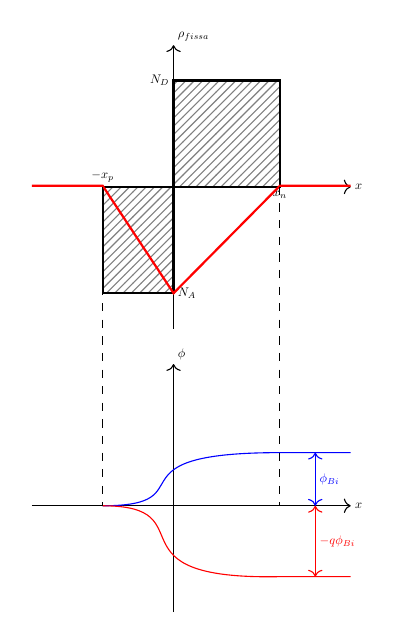
\begin{tikzpicture}[scale=0.45,transform shape]
         %disegno asse x
        \draw[->] (-4,0) node[anchor=north]{}--++ (9,0)
        node[anchor=west]{$x$};
        %disegno asse y
        \draw[->] (0,-4)--++ (0,8) node[anchor=south west]{$\rho_{fissa}$};
        %disegno grafici
        \draw[thick,pattern=north east lines, pattern color=gray] (0,0)rectangle++ (3,3);
        \draw[thick,pattern=north east lines, pattern color=gray] (0,0)rectangle++ (-2,-3);
        %label
        \node at (3,0) [anchor=north]{$x_n$};
        \node at (-2,0) [anchor=south]{$-x_p$};
        \node at (0,3) [anchor=east]{$N_D$};
        \node at (0,-3) [anchor=west]{$N_A$};

        %disegno l'energia
        \draw[thick,red] (-4,0.03)-- (-2,0.03)-- (0,-3)-- (3,0.03)-- (5,0.03);

        %disegno grafico potenzili
        %disegno asse x
        \draw[->] (-4,-9) node[anchor=north]{}--++ (9,0)
        node[anchor=west]{$x$};
        %disegno asse y
        \draw[->] (0,-12)--++ (0,7) node[anchor=south west]{$\phi$};
        
        %disegno graficiù
        \draw[blue] (-2,-9)..controls (1,-9) and (-2,-7.5).. (3,-7.5)--++ (2,0);
        \draw[red] (-2,-9)..controls (1,-9) and (-2,-11.1).. (3,-11)--++ (2,0);
    
        %tratteggi
        \draw[dashed] (-2,0)--++ (0,-9);
        \draw[dashed] (3,0)--++ (0,-9);
        %label
        \draw[<->,blue] (4,-9)-- (4,-7.5);
        \node at (4,-8.25)[anchor= west,blue]{$\phi_{Bi}$};
        \draw[<->,red] (4,-11)-- (4,-9);
        \node at (4,-10)[anchor= west,red]{$-q\phi_{Bi}$};
    \end{tikzpicture}
    \captionof{figure}{Caption}
\end{center}
\end{minipage}

%

Ulteriori passaggi di elettroni verso la zona P (e lacune verso la zona N) contribuiranno ad alterare la neutralità delle zone e quindi a rendere più forte il campo elettrico, il quale spinge verso destra gli elettroni e verso sinistra le lacune riducendo la corrente di diffuzione fino a trovare una situazione di equilibrio in cui la forza del campo elettrico eguaglia la spinta esercitata dalla diffusione.\\

La presenza del campo elettrico produce una differenza di potenziale a cavallo della giunzione che va via aumentando con l'aumentare delle cariche che accumulano ai lati della giunzione stessa. A destra si addensano cariche positive, emntre a sinistra cariche negative.
Questa differenza è chiamata barriera di potenziale per indicare che essa si pone come barriera ai portatori di carica soggetti alla psinta della diffuzione .
La barriera auemnta fino a quando i portatori che diffondono non sono più in grado di superarla.\\
\begin{figure}[hbt!]
    \centering
\begin{tikzpicture}[scale=0.75, transform shape]
    %disegno asse x
        \draw[->] (-5,0)--++ (10,0)
        node[anchor=west]{$x$};
        %disegno asse y
        \draw[->] (0,-1)--++ (0,5) node[anchor=south west]{$\rho_{mobile}$};
        %disegno tratteggi
        \draw[dashed] (-2,0)--++ (0,4);
        \draw[dashed] (2,0)--++ (0,4);
        %disegno grafici
        \draw[thick, red] (-5,0.5)-- (-2,0.5)  (2,0.5)-- (5,0.5);
        \draw[thick, black] (-5,3)-- (-2,3)  (2,3)-- (5,3);
        %label 
        \node at (-2,0)[below]{$-x_p$};
        \node at (2,0)[below]{$x_n$};
        
        \node at (-5,3)[left]{$N_A$};
        \node at (-5,0.5)[left]{$nP_0$};
        
        \node at (5,3)[right]{$N_D$};
        \node at (5,0.5)[right]{$Pn_0$};
\end{tikzpicture}
    \caption{Caption}%
    \label{fig:enter_label}
\end{figure}

Per costruire il diagramma a bande bisognerà ricordare che:
\begin{enumerate}
    \item la densità di elettroni e lacune dipende da $E_F$ secondo le relazioni:
            \begin{align*}
                n=N_C \cdot \exp\left (\dfrac{E_F-E_C}{k_B T} \right)\\
                p=N_V \cdot \exp\left (\dfrac{E_V-E_F}{k_B T} \right)
            \end{align*}
    \item esiste un campo elettrico nei dintorni della giunzione, indicando che le bande saranno inclinate
            In tale regione il numero di elettroni in zona n e di lacune in zona p sono sensibilmente 
            inferiori rispetto al loro valore lontano dalla giunzione (zona di svuotamento).
            
\end{enumerate}

Poiché n è esponenzialmente dipendente dalla distanza $E_C-E_F$ (e p da $E_F-E_V$) allora, nel diagramma, $E_C$ si allontana dalla zona $E_F$.
Perciò il campo elettrico fa inclinare le bande, mentre il livello di fermi resta piatto e costituisce un comodo livello di riferimento per il potenziale\\
Figura\\

Per quanto abbiamo detto, Il diagramma a bande in equilibrio termodinamico rivela che in corrispondenza della giunzione vi è un campo elettrico di built-in;
questo contrasta la tendenza degli elettroni a diffondersi dal lato n al lato p e delle lacune a diffondersi dal lato p al lato n, in modo tale da rendere nulla la corrente totale, come richiesto dalla condizione di equilibrio termodinamico.

Pertanto, la corrente di deriva indotta dal campo di built in compensa esattamente la corrente di diffusione indotta dai gradienti di concentrazione dei portatori.

quando si uniscono si una una cetra concentrazione di ioni fissi:\\
fig\\

il campo elettrico sarà\\
fig\\
La conseguenza della presenza del campo elettrico è l'esistenza di un potenziale. Sappiamo infatti che esso è legato al campo elettrico dall'equazione
\begin{equation}
    \mathcal{\vec{E}}(x)=-\nabla V(x)
\end{equation}
Considerando l'impotesi modonimensionale:
\begin{equation}
    \mathcal{\vec{E}}(x)=-\dfrac{V(x)}{dx}
\end{equation}

Da cui 
\begin{equation}
    V(x)= \int_{-\infty}^{x}\mathcal{\vec{E}}(x)dx
\end{equation}

All'equilibrio termodinamico tra i due lati della giunzione si ha una differenza di potenziale Vbi. Come si calcola?

Il valore Vbi si può dedurre imponendo che la densitò di corrente per gli elettroni si annilli all'equilibrio termico
\begin{equation}
    J_n=J_{n,Deriva} + J_{n,Diffusione} = q \mu_n n \mathcal{\vec{E}}(x) +qD_n \dfrac{dn}{dx}
\end{equation}

Il che implica
\begin{equation}
    \mathcal{\vec{E}}(x) = - \dfrac{D_n}{\mu_n} \dfrac{1}{n} \dfrac{dn}{dx}= -\dfrac{KT}{q}\dfrac{1}{n} \dfrac{dn}{dx}
\end{equation}

Da cui si può ricavare Vbi
\begin{equation}
   % V_bi=-∫_(-∞)^(+∞)▒E(x)  dx=KT/q ln((N_D N_A)/(n_i^2 ))
\end{equation}


\subsection{DIAGRAMMA A BANDE IN POLARIZZAZIONE DIRETTA}
In equilibrio termodinamico sottoponiamo la giunzione pn a polarizzazione diretta, ossia applichiamo al lato p un potenziale positivo, mantenendo il lato n al potenziale di riferimento.
Di seguito considereremo il caso di filo ideale. l'intera tensione fornita dal generatore cade sulla regione di carica spaziale.

Se il lato p è polarizzato positivamente, l'energia potenziale del mezzo p diminuisce.
Supponendo di mantenere come riferimento il livello delle bande del lato n, la tensione applicata $V_A>0$ riduce la barriera di potenziale a XX causando una riduzione del campo di built in
\begin{figure}[hbt!]
    \centering
    \begin{tikzpicture}
    %disegno asse x
        \draw[->] (-5,0)--++ (10,0)
        node[anchor=west]{$x$};
        %disegno asse y
        \draw[->] (0,-1)--++ (0,5) node[anchor=south west]{$\rho_{mobile}$};
        %disegno tratteggi
        \draw[dashed] (-2,0)--++ (0,4);
        \draw[dashed] (2,0)--++ (0,4);
        %disegno grafici
        \draw[thick, red] (-5,0.5)-- (-2,0.5)  (2,0.5)-- (5,0.5);
        \draw[thick, black] (-5,3)-- (-2,3)  (2,3)-- (5,3);
        %collegamenti
        \draw[blue] (-2,3)..controls (-0.5,3) and (0.5,0.5).. (2,0.5);
        \draw[green] (-2,0.5)..controls (-0.5,0.5) and (0.5,3).. (2,3);
        %label 
        \node at (-2,0)[below]{$-x_p$};
        \node at (2,0)[below]{$x_n$};
        
        \node at (-5,3)[left]{$N_A$};
        \node at (-5,0.5)[left]{$nP_0$};
        
        \node at (5,3)[right]{$N_D$};
        \node at (5,0.5)[right]{$Pn_0$};
\end{tikzpicture}
    \caption{Caption}%
    \label{fig:enter_label}
\end{figure}
%
\begin{figure}[hbt!]
    \centering
    \begin{tikzpicture}
    %disegno asse x
        \draw[->] (-5,0)--++ (10,0)
        node[anchor=west]{$x$};
        %disegno asse y
        \draw[->] (0,-1)--++ (0,5) node[anchor=south west]{$\rho_{mobile}$};
        %disegno tratteggi
        \draw[dashed] (-2,0)--++ (0,4);
        \draw[dashed] (2,0)--++ (0,4);
        %disegno grafici
        \draw[thick, red] (-5,0.5)-- (-2,0.5)  (2,0.5)-- (5,0.5);
        \draw[thick, black] (-5,3)-- (-2,3)  (2,3)-- (5,3);
        %collegamenti
        \draw[blue] (-2,3)..controls (0.5,3) and (-0.5,0.5).. (2,0);
        \draw[blue] (2,0)..controls (3,0) and (3.7,0.5).. (5,0.5);
        
        \draw[green] (-2,0)..controls (0,0.5) and (0,3).. (2,3);
        \draw[green] (-5,0.5)..controls (-3.7,0.5) and (-3,0).. (-2,0);
        %label 
        \node at (-2,0)[below]{$-x_p$};
        \node at (2,0)[below]{$x_n$};
        
        \node at (-5,3)[left]{$N_A$};
        \node at (-5,0.5)[left]{$nP_0$};
        
        \node at (5,3)[right]{$N_D$};
        \node at (5,0.5)[right]{$Pn_0$};
\end{tikzpicture}
    \caption{Caption}%
    \label{fig:enter_label}
\end{figure}
\cleardoublepage%

\section*{09/10/2023}

\subsection{Tensione di built-in (analisi quantitativa) pg 265}
Considero di avere una giunzione fra due semiconduttori con elevato drogaggio, cioè con drogaggio molto maggiore di quello che ci sarebbe in n semiconduttore intrinseco. il semiconduttore P avrà livello di fermi molto minore di quello intrinseco mentre il semiconduttore N avrà un livello di fermi molto maggiore.
utilizzando la forma di Shockley (ossia prendendo come riferimento per il potenziale il livello di Fermi intrinseco), si ha:

\begin{align*}
    n_0(x)=n_i \cdot \exp\left (\dfrac{E_F-E_{Fi}(x)}{k_B T} \right)\\
    p_0(x)=n_i \cdot \exp\left (\dfrac{E_{Fi}(x)-E_F}{k_B T} \right)
 \end{align*}\\
 Dove il pedice "0" indica la condizione di equilibrio termodinamico.\\
 Lontano dalla giunzione, le concentrazioni di elettroni e lacune sono, rispettivamente, circa uguali alle concentrazioni di donatori e accettori. Per cui valgono le relazioni:
\begin{align}
    n(\infty)=N_D=n_i \cdot \exp\left (\dfrac{E_F-E_{Fi}(+\infty)}{k_B T} \right)\\
    p(\infty)=N_A=n_i \cdot \exp\left (\dfrac{E_{Fi}(-\infty)-E_F}{k_B T} \right)
 \end{align}
Estrapolando i livelli energetici presenti all'esponenziale, ottengo:
 \begin{align}
     E_F-E_{Fi}(+\infty) = k_B T \log \left({\dfrac{N_D}{n_i}} \right)\\
     E_{Fi}(-\infty)-E_F = k_B T \log \left({\dfrac{N_A}{n_i}} \right)
 \end{align}\\
Se ora facciamo la somma di queste due equazioni (e $V_A=0$), trovo:
 \begin{equation}
     qV_{bi}=E_{Fi}(-\infty)-E_{Fi}(+\infty)=k_B T \log \left( \dfrac{N_D N_A}{n_i^2}\right)
 \end{equation}\\
Mettendo tutto insieme trovo:
 \begin{align}
 \label{eqn:Vbi}
      V_{bi}= \dfrac{k_B T}{q}\log \left( \dfrac{N_D N_A}{n_i^2}\right)
 \end{align}

Dall'espressione della $V_{bi}$ capisco che, fissato il semiconduttore intrinseco, la barriera di potenziale dipende dalla concentrazione dei droganti e dalla temperatura del sistema.

 \begin{ricevimento}
     perchè negli appunti ho scritto:
     \begin{equation}
         n(-\inf) \cdot p(+\inf)=V_{bi}
     \end{equation}
     ??
 \end{ricevimento}
 \cleardoublepage%
La cosa interessante avviene quando il potenziale esterno non è più nullo ($V_A \neq 0$). il risultato è rappresentato nella seguente figura:

\begin{figure}[hbt!]
    \centering
     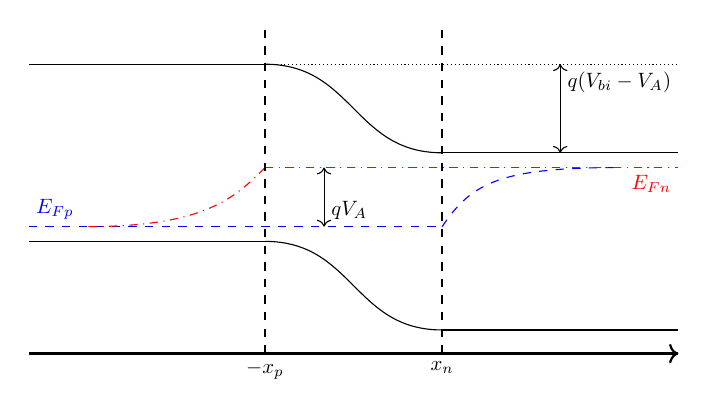
\begin{tikzpicture}[scale=0.75, transform shape]
        %disegno l'unione di due SC
        %asse x e label
        \draw[thick] (0,-1.9) --++ (4,0) node[anchor=north]{$-x_p$}--++ (3,0) node[anchor=north]{$x_n$}--++ (4,0);
        \draw[thick,->] (10.9,-1.9)--++ (0.1,0);
        %mezzo 1
        \draw(0,3) --++ (4,0);
        \draw(0,0) --++ (4,0);
        %mezzo 2
        \draw(7,1.5) --++ (4,0);
        \draw(7,-1.5) --++ (4,0);
        %livelli di fermi
        \draw[dashed,blue] (0,0.25) node[anchor=south west]{$E_{Fp}$} --++ (7,0);
        \draw[dashed, blue ] (7,0.25)..controls (7.5,1) and (8,1.25).. (10,1.25);
        
        \draw[dash dot,red] (4,1.25) --++ (7,0) node[anchor=north east]{$E_{Fn}$};
        \draw[dash dot,red] (4,1.25)..controls (3.5,0.75) and (3,0.25).. (1,0.25);
        %intersezione
        \draw[] (4,3)..controls (5.5,3) and (5.5,1.5).. (7,1.5);
        \draw[] (4,0)..controls (5.5,0) and (5.5,-1.5).. (7,-1.5);
        %delimitazioni
        \draw[thick, dashed] (4,-1.9)--++ (0,5.5);
        \draw[thick, dashed] (7,-1.9)--++ (0,5.5);
        %altro
        \draw[<->] (5,1.25)-- (5,0.25) node[anchor=south west]{$qV_A$};
        \draw[densely dotted] (4,3)--++ (7,0);
        \draw[<->] (9,3) node[anchor=north west]{$q(V_{bi}-V_A)$}-- (9,1.5);
    \end{tikzpicture}
    \caption{Caption}%
    \label{fig:enter_label}
\end{figure}
Quando il potenziale applicato $V_A \neq 0$, i livelli di fermi dei due semiconduttori non combaciano più ma sono traslati e prendono il nome di "livelli di Quasi-Fermi ($E_{fp}$ ed $E_{fn}$)". la traslazione dei i due livelli è proporzionale all'energia potenziale $qV_A$ e quindi alla tensione $V_A$.\\
Per continuare la trattazione si definiscono i seguenti parametri:
 \begin{enumerate}
     \item $p(-x_p) \approx N_A$ è la condentrazione delle lacune nel lato p, circa costante fino ai limiti della zona di svuotamento (vale anche in condizioni di non equilibrio, purchè si abbia basso livello di iniezione);
     \item $n(-x_p)$ è la concentrazione degli elettroni (portatori minoritari) nel lato p ai limiti della zona di svuotamento;
     \item $x(x_n) \approx N_D$ è la condentrazione degli elettroni nel lato n, circa costante fino ai limiti della zona di svuotamento (vale anche in condizioni di non equilibrio, purchè si abbia basso livello di iniezione);
     \item $p(x_n)$ è la concentrazione delle lacune (portatori minoritari) nel lato n ai limiti della zona di svuotamento;
 \end{enumerate}
Per calcolare il valore della concentrazione dei portatori minoritari ricordo che $n(x) \cdot p(x) =n_i^2$, allora:
 \begin{align*}
     n_0(-x_p) &= \dfrac{n_i^2}{N_A}\\
     p_0(x_n)  &= \dfrac{n_i^2}{N_D}
 \end{align*}\\
 Unendo le considerazioni fatte con l'equazione n.\ref{eqn:Vbi}, ottengo che la concentrazione dei portatori minoritari ai limiti della regione di svuotamento è legata, all'equilibrio termodinamico, alla concentrazione dei portatori maggioritari al limite opposto:
 \begin{align}
     p_0(x_n)=p_0(-x_p) \exp \left( -\dfrac{V_{bi}}{V_T} \right)\\
     n_0(-x_p)=n_0(x_n) \exp \left( -\dfrac{V_{bi}}{V_T} \right)
 \end{align}

\cleardoublepage%
\subsection{Corrente totale nella giunzione pn}
La giunzione che stiamo trattando è bipolare, cioè la corrente che si instaura è costituita sia da elettroni che da lacune. Quindi la corrente totale è formata da quattro componenti ovvero trascinamento e diffusione di elettroni + trascinamento e diffusione di lacune:
\begin{equation}
    J = J_{n,t} + J_{n,d} + J_{h,t} + J_{h,d}
\end{equation}

Ora considero 2 ipotesi principali (ed una implicita):
\begin{enumerate}
    \item Alcune delle quattro componenti sono trascurabili nel lato n o p: per bassi livelli di iniezione \textit{(e quindi per basso $\mathcal{\vec{E}}$ che si instaura) si possono trascurare le correnti di trascinamento dei portatori minoritari rispetto alle correnti di trascinamento dei portatori maggioritari.}
    \begin{psbox}[PS]
                E' importante ricordare che la corrente di trascinamento dipende dal campo elettrico. Affinchè la corrente di trascinamento dei portatori maggioritari sia maggiore di quella dei minoritari \textbf{è necessario che ci sia un minimo di campo !}. altrimenti sarebbero tutti a zero.
            \end{psbox}
    
    \item \textit{il tasso di generazione e ricombinazione nella regione svuotata è trascurabile, e quindi le densità totali di corrente di elettroni e di lacune sono costanti nella regione svuotata.}
    
    \item (implicita) la regione non svuotata è elettricamente neutra (\textbf{o quasi neutra})
            
\end{enumerate}
La regione svuotata si trova tra le coordinate ($-x_p$ e $x_n$) poichè in campo elettrico in questa regione è diversa da zero, mentre altrove vige la quasi neutralità delle cariche ($\dfrac{dQ}{dt}\approx 0$).\\
\textbf{Per la 1° ipotesi}, la corrente dei portatori minoritari (fatta di elettroni in regione p e lacune in regione n) è costituita solo da componenti diffusive.
\begin{align*}
    J_n &\approx J_{n,d} &&\text{per } x \leq -x_p \text{ (lato p) }\\
    J_h &\approx J_{h,d} &&\text{per } x \geq x_n \text{ (lato n) }
\end{align*}
\begin{citbox}
    In particolare, ai limiti della regione di carica spaziale si ha:
    \begin{align}
        J_n(-x_p)&=J_{n,d}(-x_p)\\
        J_h(x_n) &=J_{h,d}(x_n)
    \end{align}
\end{citbox}\leavevmode\newline
Quindi, nel  caso di basso campo elettrico, la corrente totale nei lati p ed n si scrive:
\begin{align*}
    J^{tot} &\approx J_{n,d} + J_h &&\text{per } x \leq -x_p \text{ (lato p) }\\
    J^{tot} &\approx J_{h,d} + J_n &&\text{per } x \geq x_n \text{ (lato n) }
\end{align*}\\
\textbf{Per la 2° ipotesi}, la corrente di elettroni (lacune) misurata al limite destro (sinistro) della regione svuotata è identica alla corrente nel limite sinistro (destro):
\begin{align*}
    J_n(x_n)&=J_n(-x_p)\\
    J_h(x_n) &=J_h(-x_p)
\end{align*}
Dall'equazione di continuità si perviene che la $J^{tot}$ è costante in tutte le sezioni indipendentemente da x, ovvero:
\begin{align*}
    \dfrac{dQ}{dt} &+\dfrac{dJ}{dx}+G-R=0 \\
    0              &+\dfrac{dJ}{dx}+0+0=0 
\end{align*}
Dato che la corrente totale $J^{tot}$ del diodo è costante sezione per sezione, posso pensare di calcolarla in un punto a mio piacere, ovvero nel punto $x_n$:
\begin{equation*}
    J^{tot}=J(x_n)=J_n(x_n)+J_h(x_n)=J_n(-x_p)+J_h(x_n)=J_{n,d}(-x_p)+J_{h,d}(x_n)
\end{equation*}
Il risultato che si ottiene è che la densità di corrente totale è funzione delle correnti di diffusione di elettroni e lacune:
\begin{equation}
    J^{tot}=J_{n,d}(-x_p)+J_{h,d}(x_n)
\end{equation}
Valutando la corrente in $-x_p$ si ottiene la stessa equazione:
\begin{equation*}
    J^{tot}=J(-x_p)=J_n(-x_p)+J_h(-x_p)=J_n(-x_p)+J_h(x_n)=J_{n,d}(-x_p)+J_{h,d}(x_n).
\end{equation*}
E quindi
\begin{equation*}
    J^{tot}=J_{n,d}(-x_p)+J_{h,d}(x_n).
\end{equation*}
Pertanto,avendo trascurato l'effetto della ricombinazione e generazione nella regione di svuotamento, \textbf{la corrente totale di una giunzione si valuta sommando le correnti di diffusione dei portatori minoritari iniettati nei due lati della giunzione ai limiti della regione di carica spaziale}.\\
%
Ora voglio calcolare analiticamente queste correnti.
%
\textbf{Concentrazione dei portatori minoritari in eccesso}\\
Per calcolare le correnti di diffusione dei portatori minoritari iniettati in $-x_p,x_n$ è necessario \textbf{stimare la concentrazione dei portatori minoritari in eccesso ai limiti della regione di svuotamento.}:
\begin{equation}
    J^{tot}=J_{n,d}(-x_p)+J_{h,d}(x_n) = qD_n \left. \dfrac{dn}{dx}\right|_{-x_p} -qD_h \left. \dfrac{dp}{dx}\right|_{x_n}
\end{equation}
da cui
\begin{equation}
    J^{TOT}= qD_n \left. \dfrac{dn'}{dx}\right|_{-x_p} -qD_h \left. \dfrac{dp'}{dx}\right|_{x_n}
\end{equation}

In presenza di una polarizzazione applicata (cioè fuori dall'equilibrio termodinamico) è possibile, almeno in basso livello di iniezione, assumenre come costanti i quasi-livelli di Fermi di elettroni e lacune nella regione di carica spaziale.

Tenendo presente che
\begin{equation}
    p \cdot n = {n_i}^2 \cdot \exp\left( \dfrac{E_{Fn} - E_{Fh}}{k_B T} \right) \quad \text{for} \quad -x_p \leq x \leq x_n
\end{equation}

 e che $E_{Fn}-E_{Fh}=qV_A$, si ottiene:
\begin{align}
    p(x_n)\cdot n(x_n)&=n_i^2 \exp\left( \dfrac{V_A}{V_T}\right)\\
    p(-x_p)\cdot n(-x_p)&=n_i^2 \exp\left( \dfrac{V_A}{V_T}\right)
\end{align}

Supposto che per basso livello di iniezioni, la concentrazione dei portatori maggioritari non vari in modo apprezzabile rispetto all'equilibrio:
\begin{align}
    n(x_n)&=N_D\\
    p(-x_p)&=N_A
\end{align}
si ricava:
\begin{align}
    p(x_n)&=\dfrac{n_i^2}{N_D} \exp\left( \dfrac{V_A}{V_T}\right)\\
    n(-x_p)&=\dfrac{n_i^2}{N_A} \exp\left( \dfrac{V_A}{V_T}\right)
\end{align}
\begin{center}
    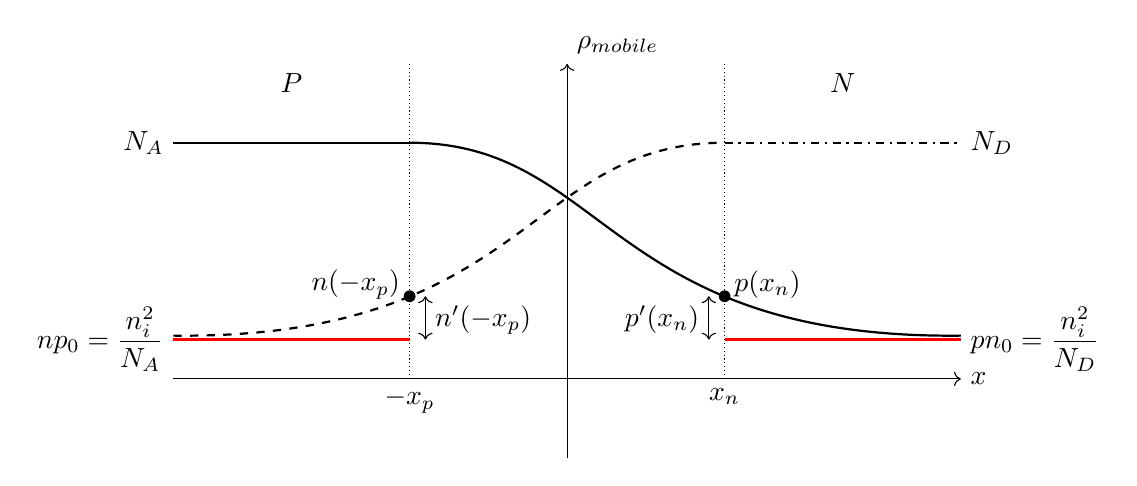
\begin{tikzpicture}
        [circle dotted/.style={dash pattern=on .05mm off 8mm, line cap=round}]
        %disegno asse x
            \draw[->] (-5,0)--++ (10,0)
            node[anchor=west]{$x$};
            %disegno asse y
            \draw[->] (0,-1)--++ (0,5) node[anchor=south west]{$\rho_{mobile}$};
            %disegno tratteggi
            \draw[densely dotted] (-2,0)--++ (0,4);
            \draw[densely dotted] (2,0)--++ (0,4);
            %disegno grafici
            \draw[thick, red] (-5,0.5)-- (-2,0.5)  (2,0.5)-- (5,0.5);
            \draw[thick, black] (-5,3)-- (-2,3) ; 
            \draw[thick, dash dot] (2,3)-- (5,3);
            %collegamenti
            \draw[thick] (-2,3)..controls (0.5,3) and (0.5,0.5).. (5,0.55);
            \draw[thick,dashed] (-5,0.55)..controls (-0.5,0.5) and (-0.5,3).. (2,3);
            %label 
            \node at (-3.5,4)[below]{$P$};
            \node at (3.5,4)[below]{$N$};
            
            \node at (-2,0)[below]{$-x_p$};
            \node at (2,0)[below]{$x_n$};
            
            \node at (-5,3)[left]{$N_A$};
            \node at (-5,0.5)[left]{$np_0=\dfrac{n_i^2}{N_A}$};
            
            \node at (5,3)[right]{$N_D$};
            \node at (5,0.5)[right]{$pn_0=\dfrac{n_i^2}{N_D}$};

            \draw[line width = 1.5mm,circle dotted] (-2,1.05) --++ (0,0);
            \node at (-2,1.2)[left]{$n(-x_p)$};
            \draw[line width = 1.5mm,circle dotted] (2,1.05) --++ (0,0);
            \node at ((+2,1.2)[right]{$p(x_n)$};

            \draw[<->] (-1.8,0.5)-- (-1.8,1.05) node[anchor=north west]{$n'(-x_p)$};
            \draw[<->] (1.8,0.5)-- (1.8,1.05) node[anchor= north east]{$p'(x_n)$};
    \end{tikzpicture}
\end{center}

Siccome voglio calcolare la corrente che si forma a seguito dell'iniezione dei portatori in eccesso, dovrò prendere l'equazione della concentrazione totale, calcolato nel particolare punto di interesse, e sottrargliil corrispettivo $\dfrac{n_i^2}{N}$ che si avrebbe all'equilibrio fuori dalla regione di svuotamento.:

\begin{align}
    p'(x_n)&=\dfrac{n_i^2}{N_D} \left[ \exp\left( \dfrac{V_A}{V_T}\right) -1 \right]\\
    n'(-x_p)&=\dfrac{n_i^2}{N_A} \left[\exp\left( \dfrac{V_A}{V_T}\right) -1 \right]
\end{align}
\begin{psbox}[Proseguendo..]
    Da libro: Se si trascura la corrente di trascinamento dei portatori minoritari, l'evoluzione della popolazione in eccesso in funzione della posizione segue la legge studiana nel caso di portatori minoritari in eccesso dovuta a bombardamento laterale di fotoni. (trascurare la corrente di trascinamento dei portatori minoritari è equivalente a trascurare il campo elettrico nell'equazione ci dontinuità dei portatori minoritari)
\end{psbox}
La concentrazione delle lacune in eccesso nel lato n e degli elettroni nel lato p (per quanto detto nel cit.BOX sopra) segue la legge:
\begin{align}
    p'(x_n)&=\dfrac{n_i^2}{N_D} \left[ \exp\left( \dfrac{V_A}{V_T}\right) -1 \right] \cdot \exp \left[\dfrac{-x+x_n}{L_{hn}} \right]\\
    n'(-x_p)&=\dfrac{n_i^2}{N_A} \left[\exp\left( \dfrac{V_A}{V_T}\right) -1 \right]\cdot \exp \left[\dfrac{x+x_p}{L_{np}} \right]\\
\end{align}
dove $L_{hn}=\sqrt{D_h\tau_{hn}}$ è la lunghezza di diffusione delle lacune nel lato n,
$L_{np}=\sqrt{D_n\tau_{np}}$ è la lunghezza di diffusione delle lacune nel lato p,
...

\begin{center}
    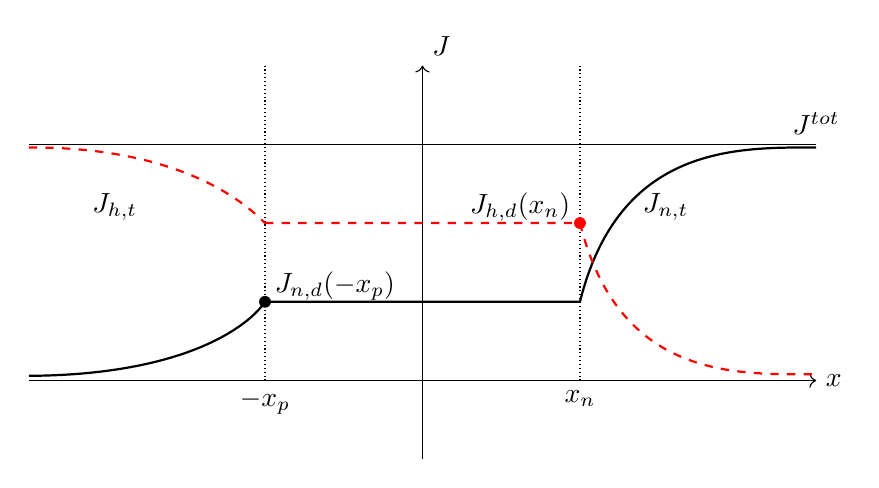
\begin{tikzpicture}
        [circle dotted/.style={dash pattern=on .05mm off 8mm, line cap=round}]
        %disegno asse x
            \draw[->] (-5,0)--++ (10,0)
            node[anchor=west]{$x$};
            %disegno asse y
            \draw[->] (0,-1)--++ (0,5) node[anchor=south west]{$J$};
            %disegno tratteggi verticali
            \draw[densely dotted] (-2,0)--++ (0,4);
            \draw[densely dotted] (2,0)--++ (0,4);
            %disegno grafici e collegamenti controls
            \draw[] (-5,3)--++ (10,0) node[anchor=south]{$J^{tot}$}; 
            \draw[thick] (-5,0.06)..controls (-3,0.07) and (-2.2,0.7).. (-2,1)
                                      (-2,1)--++ (4,0) 
                                      (2,1).. controls (2.5,3) and (4,2.96).. (5,2.96);
            \draw[thick, dashed, red]  (-5,2.96)..controls (-3,2.97) and (-2.2,2.2).. (-2,2)
                          (-2,2)--++ (4,0)   
                          (2,2).. controls (2.5,0) and (4,0.08).. (5,0.08);
            %label 
            \node at (-2,0)[below]{$-x_p$};
            \node at (2,0)[below]{$x_n$};
            
            \draw[line width = 1.5mm,circle dotted,red] (2,2) --++ (0,0);
            \draw[line width = 1.5mm,circle dotted] (-2,1) --++ (0,0);
            
            \node at (-2,1.2)[right]{$J_{n,d}(-x_p)$};
            \node at (2,2.2)[left]{$J_{h,d}(x_n)$};
            % label correnti di trascinamento portatori maggioritari
            \node at (3.5,2.2)[left]{$J_{n,t}$};
            \node at (-3.5,2.2)[left]{$J_{h,t}$};
    \end{tikzpicture}
\end{center}

La densità di corrente totale può essere ottenuta derivando rispetto ad x le concentrazioni in eccesso:
\begin{equation}
    J=\dfrac{qD_n}{L_{np}}n'(-x_p)+\dfrac{qD_h}{L{hn}}p'(x_n)
\end{equation}
ossia:
\begin{equation}
    J=qn_i^2\left( \dfrac{D_n}{N_A L{np}}+\dfrac{D_h}{N_DL{hn}} \right)\left[ \exp\left( \dfrac{V_A}{V_T}\right)-1 \right]
\end{equation}
Dove chiamo $ J_0=qn_i^2\left(\dfrac{D_n}{N_A L{np}}+\dfrac{D_h}{N_D L{hn}}\right)$ \textbf{\emph{densità di corrente inversa di saturazione}}.\\
Da notare, in realtà che l'espressione ottenuta per $J_0$ vale solo se el regioni p ed n del diodo sono lunghe rispetto alla lunghezza della diffusione ($W$).
se questo non accadesse e cioè, se la lunghezza di diffusione del lato p ($W_P$) e la lunghezza di diffusione del lato n ($W_n$) fossero paragonabili a W,la soluzione sarebbe più complessa.

per riassumere le ultime equazioni con la figura XX:
poichè il contributo della corrente di diffusione diminuisce esponenzialmente man mano che ci si allontana dal limite della regione di svuotamento, la corrente di deriva dei portatori maggioritari deve crescere in modo da mantenere costante la corrente totale

\cleardoublepage%

\section*{12/10/2023}

pg.278
\subsection{Elettrostatica della giunzione pn}
\begin{psbox}
    l'equazione di Poisson verrà risolta nella regione di svuotamento, e le dimensioni di quest'ultima ($-x_p, x_n$) verranno legate al potenziale applicato alla giunzione
\end{psbox}
Assumiamo come riferimento dell'energia potenziale il livello di Fermi intrinseco; Allora l'equazione id Poisson si scrive
\begin{equation}
    \dfrac{d^2E_{Fi}}{dx^2}=\dfrac{q\rho}{\epsilon}
\end{equation}
Lo studio che si tratterrà in seguito avrà come risultato finale le seguenti figure:\\
%
\noindent\begin{minipage}{0.6\textwidth}
    Partiamo innanzitutto considerando la densità di carica netta $\rho$:
\begin{equation}
    \rho(x) = \begin{cases}
    0&  \text{per $x < x_p$},\\
    -qN_A& \text{per $-x_p<x<0$ },\\
    qN_D& \text{per $0<x<x_n$ },\\
    0& \text{per $x>x_n$ }
\end{cases}
\end{equation}
e pertanto l'equazione di Poisson si scrive:
\begin{equation}
    \dfrac{d^2E_{F_i}}{dx^2} = \begin{cases}
    0 & \text{per $x < x_p$},\\
    -\dfrac{q^2N_A}{\epsilon}& \text{per $-x_p<x<0$ },\\
    -\dfrac{q^2N_D}{\epsilon}& \text{per $0<x<x_n$ },\\
    0 & \text{per $x>x_n$ }
\end{cases}
\end{equation}
Poichè non vi sono altre cariche presenti nel sistema, deve valere la condizione di neutralità globale \\ ($Q^+=Q^-$).\\
La carica netta totale presente deve quindi essere nulla, il che implica che nella regione di svuotamento la carica totale positiva sia pari alla carica totoale negative:
\begin{equation}
    x_n N_D=x_p N_A
\end{equation}
Per la legge di Gauss, il campo elettrico e la tensione sono legati da una relazione integrale.\\
Ricordo che il campo è nullo all'esterno della regione di svuotamento per la condizione di neutralità e quindi,  integrando una volta l'equazione di Poisson, si ottiene:
\begin{equation}
    \dfrac{dE_{F_i}}{dx} = \begin{cases}
    0 & \text{per $x < x_p$},\\
    -\dfrac{q^2N_A}{\epsilon} x + A & \text{per $-x_p<x<0$ },\\
    -\dfrac{q^2N_D}{\epsilon} x + B & \text{per $0<x<x_n$ },\\
    0 & \text{per $x>x_n$ }
\end{cases}
\end{equation}
\end{minipage}
\hfill%
\begin{minipage}{0.35\textwidth}\raggedleft
    \begin{center}
    \begin{tikzpicture}[scale=0.5]
             %disegno asse x
            \draw[->] (-5,2) node[anchor=north]{}-- (5,2)
            node[anchor=west]{$x$};
            %disegno asse y
            \draw[->] (0,-1.5)-- (0,5) node[anchor=south west]{$\rho_{fissa}(x)$};
            %disegno grafici
            \draw[thick,pattern=north east lines, pattern color=gray] (0,2)rectangle++ (4,2);
            \draw[thick,pattern=north east lines, pattern color=gray] (0,2)rectangle++ (-3,-2.5);
            %label
            \node at (4,2) [anchor=north]{$x_n$};
            \node at (-3,2) [anchor=south]{$-x_p$};
            \node at (0,4) [anchor=east]{$qN_D$};
            \node at (0,-4.5) [anchor=west]{$-qN_A$};
            \node at (2,3) [red]{$Q^+$};
            \node at (-1.5,0.75) [red]{$Q^-$};

            %disegno grafico energia
            %disegno asse x
            \draw[->] (-5,-5.5) node[anchor=north]{}-- (5,-5.5)
            node[anchor=west]{$x$};
            %disegno asse y
            \draw[->] (0,-9.5)-- (0,-3.7) node[anchor= west]{$\mathcal{E}(x)$};
            %disegno grafico rosso
            \draw[thick,red] (-5,-5.5)-- (-3,-5.5)-- (0,-9)-- (4,-5.5)-- (5,-5.5);
            %label
            \node at (0,-9) [anchor=west]{$\mathcal{E}_{MAX}$};

            %disegno grafico potenziale
            %disegno asse x
            \draw[->] (-5,-12.5) node[anchor=north]{}--++ (10,0)
            node[anchor=west]{$x$};
            %disegno asse y
            \draw[->] (0,-15.5)-- (0,-11.7) node[anchor= west]{$\phi(x)$};
            %disegno grafico rosso
            \draw[thick] (-5,-12.5)--++ (2,0).. controls (1,-12.5) and (-0,-15.7) .. (4,-15.5)--++ (1,0);
            \draw[<->] (4,-15.5)-- (4,-12.5);
            \node at (4,-14)[anchor=west]{$q(V_{bi}-V_A)$};
            %label
            \node at (0,-9) [anchor=west]{$\mathcal{E}_{MAX}$};
    \end{tikzpicture}
\end{center}
\end{minipage}


Ma il campo deve essere continuo in $x$, per cui $x=-x_p$ la derivata del livello di Fermi intrinseco si deve annullare, e così per $x=x_n$. Allora:
\begin{align*}
    -\dfrac{q^2N_A}{\epsilon} x_p + A = 0
\end{align*}
da cui:
\begin{align*}
    A = \dfrac{q^2N_A}{\epsilon} x_p
\end{align*}
    Analogamente, nel punto $x_n$:
\begin{align*}
     \dfrac{q^2N_D}{\epsilon} x_n + B =0
\end{align*}
   da cui:
\begin{align*}
     B = -\dfrac{q^2N_D}{\epsilon} x_n
\end{align*}
Questo porta alla soluzione
\begin{equation}
    \dfrac{dE_{F_i}}{dx} = \begin{cases}
    0 & \text{per $x < x_p$},\\
    -\dfrac{q^2N_A}{\epsilon} (x + x_p) & \text{per $-x_p<x<0$ },\\
    -\dfrac{q^2N_D}{\epsilon} (x - x_n ) & \text{per $0<x<x_n$ },\\
    0 & \text{per $x>x_n$ }
\end{cases}
\end{equation}

Adesso integro un'ultima volta, considerando l'equazione di neutralità globale:

\begin{equation}
    E_{F_i}= \begin{cases}
    A & \text{per $x < x_p$},\\
    -\dfrac{q^2N_A}{2\epsilon} {(x + x_p)}^2 + B& \text{per $-x_p<x<0$ },\\
    -\dfrac{q^2N_D}{2\epsilon} {(x - x_p)}^2 + C& \text{per $0<x<x_n$ },\\
    D & \text{per $x>x_n$ }
\end{cases}
\end{equation}
Ora mi servono delle condizioni a contorno. Supponiamo di assumere come riferimento dell'energia potenziale il lato sinistro della giunzione. Si ha allora:
\begin{equation}
    E_{Fi}= \begin{cases}
        0 & \text{ per $x<-x_p$},\\
        -q(V_{bi}-V_A) & \text{ per $x>x_n$}
    \end{cases}
\end{equation}
Imponendo la prima condizione si ha subito A=0.\\
La continuità dell'energia potenziale in $x=-x_p$ fornisce B=0;\\
per $x=0$ si ottiene 

\begin{align}
    E_{Fi}(0^-)=-q^2\dfrac{N_A}{2\epsilon}x_p^2 &=E_{Fi}(0^+)=q^2\dfrac{N_D}{2\epsilon}x_n^2 + C
\end{align}
da cui:
\begin{align}
    C= -q^2\dfrac{N_D}{\epsilon}x_n^2 &- q^2\dfrac{N_D}{\epsilon}_n^2 = -q(V_{bi-V_A})
\end{align}

sapendo che $\mathcal{\vec{E}}(x=0)=N_a \cdot x_p = N_D \cdot x_n$ si perviene alla profondità di diffusione:

\begin{align}
    x_n&= \sqrt{\dfrac{2\epsilon N_{eq}(V_{bi}-V_A)}{qN_D^2}}\\
    x_p&= x_n\dfrac{N_D}{N_A}= \sqrt{\dfrac{2\epsilon N_{eq}(V_{bi}-V_A)}{qN_A^2}}
\end{align}
Dove $\dfrac{1}{N_{eq}}= \dfrac{1}{N_D} + \dfrac{1}{N_A}$.\\

L'estensione totale $X_n + x_p$ della regione di svuotamento aumenta in polarizzazione inversa e diminuisce in polarizzazione diretta, fino ad annullarsi (teoricamente) per $V_A=V_{bi}$.\\
L'estensione della regione di svuotamento è tanto minore quanto maggiore è il drogaggio;
inoltre, l'estensione della regione di svuotamento nel lato meno drogato della giunzione è maggiore di quella nel lato più drogato.\\

è importante notare che il campo elettrico massimo si ha nel punto x=0:
\begin{equation}
    \mathcal{\vec{E}}_{MAX}=-q^2\dfrac{N_A}{\epsilon}x_p=-q^2\dfrac{N_D}{\epsilon}x_n
\end{equation}
\subsection{Circuito equivalente di un diodo pn}
\begin{psbox}[\small{ QUAL'E' LA DIFFERENZA TRA LA CAPACITA' DI UN CONDENSATORE E QUELLA DI UNA GIUNZIONE PN? }]
    In un normale condensatore, la capacità è creata da due piastre conduttrici separate da un materiale dielettrico. La carica è immagazzinata nel dielettrico e la capacità è determinata dalla superficie delle piastre, dalla distanza tra loro e dalle proprietà del materiale dielettrico.\\
    
    \textbf{applicare un potenziale positivo su una delle armature del condensatore provoca un accumulo di cariche positive (+q) su quest'ultima e viceversa accade per il terminale negativo.}\\
    In questo modo si crea un accumulo di cariche: + q nel lato positivo della batteria e -q nel lato negativo della batteria.
    I valori assoluti delle quantità +q e - q sono identiche identiche e vale la relazione  $C=Q/V$
    \begin{center}
        \begin{tikzpicture}[scale=0.65,transform shape]
        % condensatore
            \draw(0,0) node[anchor=east]{$+V$}-- (2,0);
            \draw(2,1) node[anchor=south]{$+q$}-- (2,-1);
            \draw(3,1) node[anchor=south]{$-q$}-- (3,-1);
            \draw(3,0)-- (5,0) node[anchor=west]{$-V$};
        \end{tikzpicture}
    \end{center}
    In un diodo a giunzione PN, la capacità si forma a causa del drogaggio che porta alla formazione della regione di svuotamento.
    A seconda del drogaggio, potro avere una regione -q a sinistra e +q a destra, o viceversa.\\ \textbf{Nel diodo il segno delle cariche non dipende dal potenziale a cui è applicato ma dal drogaggio!}. Le cariche -q e +q sono diverse in modulo e segno.
    \begin{center}
        \begin{tikzpicture}[scale=0.65,transform shape]
            % giunzione
            \draw(0,0) node[anchor=east]{$?$}-- (1.5,0);
            \draw(1.5,1) rectangle ++ (1,-2);
            \draw(2.5,1) rectangle ++ (1,-2);
            \draw(3.5,0)-- (5,0) node[anchor=west]{$?$};
            %label
            \node at (2,0) []{$Q^-$};
            \node at (3,0) []{$Q^+$};
        \end{tikzpicture}
    \end{center}
    per approfondire, quando il diodo è polarizzato inversamente la regione di svuotamento si allarga e agisce come un dielettrico con una certa capacità. La larghezza della regione di svuotamento influisce sulla capacità di giunzione. È essenzialmente una funzione della tensione applicata al diodo e delle proprietà del materiale semiconduttore.
    Nel caso del diodo, si avrà che \[ C = \dfrac{dQ}{dV_A}\]
\end{psbox}

Il diodo pn possiede, non a caso, le caratteristiche di un condensatore: è in grado di accumulare carica elettrica e, se sottoposto a sorgente variabile, il diodo pn non risponde istantaneamente ma mostra un comportamento tipico di un bipolo reattivo.\\
Nella giunzion pn si accumula carica in due regioni:
\begin{enumerate}
    \item carica fissa nella regione di svuotamento
    \item carica mobile in eccesso o in difetto nelle regioni in cui i portatori minoritari in eccesso vengono iniettati
\end{enumerate}
La carica presente nella regione di svuotamento dipende in modo istantaneo dalla tensione applicata dala giunzione, al contrario la carica iniettata in eccesso dipende dalla tensione istantanea solo per variazioni sufficientemente lente della tensione.
\cleardoublepage%

\subsubsection*{Capacità di giunzione}
La regione di svuotamento di una giunzione PN è costituita da uno strato di ioni fissi negativi nella regione drogata p, e ioni fissi negativi nella regione drogata N.
\begin{center}
    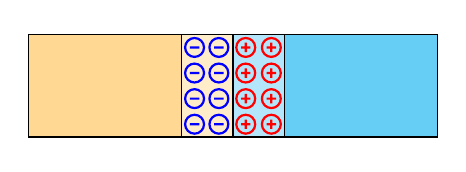
\begin{tikzpicture}[scale=0.65]
        \draw[fill=orange!60] (0,0) rectangle++ (3,2);
        \draw[fill=orange!30] (3,0) rectangle++ (1,2);
        \draw[fill=cyan!30] (4,0) rectangle++ (1,2);
        \draw[fill=cyan!60] (5,0) rectangle++ (3,2);
        %ioni negativi
        \foreach \pos in {0.25,0.75,1.25,1.75} {
        \node at (3.25,\pos) { \tikz\draw[thick,blue, scale=0.75]
        circle (0.16cm) (-0.08,0)-- (0.08,0) ;};}
        \foreach \pos in {0.25,0.75,1.25,1.75} {
        \node at (3.725,\pos) { \tikz\draw[thick,blue, scale=0.75]
        circle (0.16cm) (-0.08,0)-- (0.08,0) ;} ;}
        %ioni positivi
        \foreach \pos in {0.25,0.75,1.25,1.75} {
        \node at (4.25,\pos) { \tikz\draw[thick,red, scale=0.75]
        circle (0.16cm) (-0.08,0)-- (0.08,0) (0,0.08)-- (0,-0.08) ;} ;}
        \foreach \pos in {0.25,0.75,1.25,1.75} {
        \node at (4.75,\pos) { \tikz\draw[thick,red, scale=0.75]
        circle (0.16cm) (-0.08,0)-- (0.08,0) (0,0.08)-- (0,-0.08) ;} ;}
    \end{tikzpicture}
\end{center}

la concentrazione di questi ioni è tale per cui la carica positiva totale è uguale alla carica negativa totale.\\
Nel caso generale studiato in classe, la carica positiva è data da:
\begin{equation}
    Q_j = qAx_n N_D=|-qAx_p N_A|=A\sqrt{2q\epsilon N_{eq}(V_{bi}-V_A)}
\end{equation}
dove A è l'area della giunzione. Notiamo che l'unica variabile dell'equazione è $x_n(V_A)$.\\
La carica accumulata nella regione di svuotamento è quindi funzione istantanea della tensione applicata $V_A$; \\
E' possibile definire la capacità di giunzione associata alla caratteristica $Q_J (V_A) $ come:
\begin{equation}
    C_j=\left| \dfrac{dQ_j}{dV_A}\right|=A\sqrt{\dfrac{q\epsilon N_{eq}}{2(V_{bi}-V_A)}}
\end{equation}

\textbf{La capacità $C_J$ tende a decrescere durante la polarizzazione inversa a causa dell'allargamento della regione di carica spaziale}, mentre tende all'infinito quando la regione di carica spaziale scompare.

\begin{center}
    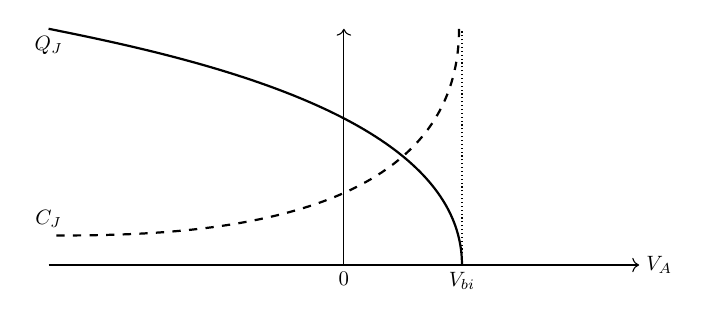
\begin{tikzpicture}[scale=0.75,transform shape]
        %disegno asse x
        \draw[->] (-5,0)--++ (10,0) node[anchor= west]{$V_A$};;
        %disegno asse x
        \draw[->] (0,0) node[anchor=north]{$0$}--++ (0,4);
        %disegno tratteggio
        \draw[densely dotted] (2,0) node[anchor=north]{$V_{bi}$}--++ (0,4);
        %disegno C_j
        \draw[thick,dashed] (1.95,4)..controls (1.95,0.5) and (-3,0.5).. (-5,0.5) node[anchor=south]{$C_J$};
        %disegno Q_j
        \draw[thick] (-5,4) node[anchor=north]{$Q_J$}..controls (-2.5,3.5) and (2,2.5).. (2,0);
    \end{tikzpicture}
\end{center}

\subsubsection*{Capacità di diffusione}
Adesso vogliamo vedere la carica mobile.\\

\begin{center}
    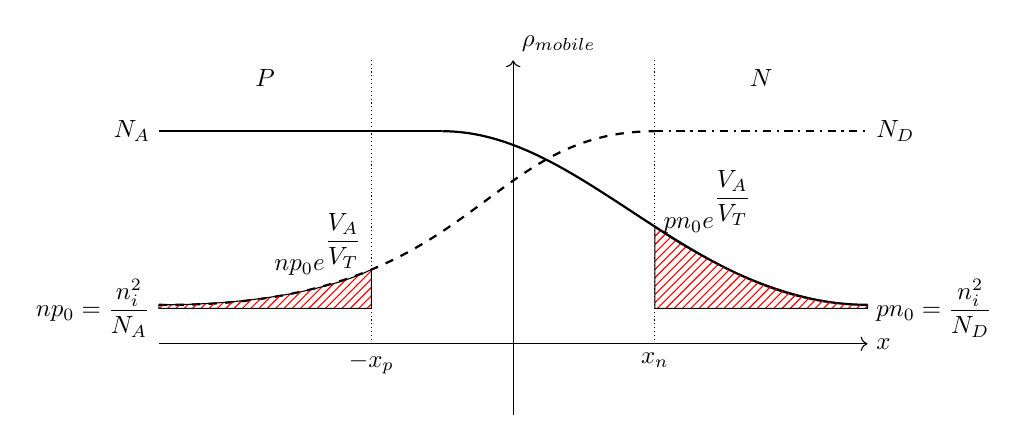
\begin{tikzpicture}[scale=0.9,transform shape]
        [circle dotted/.style={dash pattern=on .05mm off 8mm, line cap=round}]
        %disegno asse x
            \draw[->] (-5,0)--++ (10,0)
            node[anchor=west]{$x$};
            %disegno asse y
            \draw[->] (0,-1)--++ (0,5) node[anchor=south west]{$\rho_{mobile}$};
            %disegno tratteggi
            \draw[densely dotted] (-2,0)--++ (0,4);
            \draw[densely dotted] (2,0)--++ (0,4);
            %disegno grafici
            \draw[] (-5,0.5)-- (-2,0.5)  (2,0.5)-- (5,0.5);
            \draw[thick, black] (-5,3)-- (-1,3) ; 
            \draw[thick, dash dot] (2,3)-- (5,3);
            %collegamenti
            \draw[thick] (-1,3)..controls (1,3) and (2.5,0.55).. (5,0.55);
            \draw[thick,dashed] (-5,0.55)..controls (-0.5,0.5) and (-0.5,3).. (2,3);
            %label 
            \node at (-3.5,4)[below]{$P$};
            \node at (3.5,4)[below]{$N$};
            
            \node at (-2,0)[below]{$-x_p$};
            \node at (2,0)[below]{$x_n$};
            
            \node at (-5,3)[left]{$N_A$};
            \node at (-5,0.5)[left]{$np_0=\dfrac{n_i^2}{N_A}$};
            
            \node at (5,3)[right]{$N_D$};
            \node at (5,0.5)[right]{$pn_0=\dfrac{n_i^2}{N_D}$};

            \draw[line width = 1.5mm, dotted] (-2,1.05) --++ (0,0);
            \node at (-2,1.4)[left]{$np_0 e^{\dfrac{V_A}{V_T}}$};
            \draw[line width = 1.5mm, dotted] (2,1.65) --++ (0,0);
            \node at (+2,2)[right]{$pn_0 e^{\dfrac{V_A}{V_T}}$};

            % sottolineo area
            \draw[pattern=north east lines, pattern color=red] (-2,0.5)-- (-5,0.5)-- (-5,0.55)..controls (-2.9,0.55) and (-2,1.05).. (-2,1.05)-- (-2,0.5);

            \draw[pattern=north east lines, pattern color=red] (2,0.5)-- (5,0.5)-- (5,0.55)..controls (3.5,0.55) and (2,1.65).. (2,1.65)-- (2,0.5);
    \end{tikzpicture}
\end{center}

La presenza di portatori minoritari iniettati in eccesso in polarizzazione diretta, e di portatori minoritari in difetto in polarizzazione inversa, dà luogo ad un accumulo di carica esterno alla regione di svuotamento.\\
La carica totale in eccesso nel lato n (dovuta alle lacune iniettate dal lato p ) si scrive

\begin{equation}
    Q_n'=qA\int_{x_n}^{\infty} p'(x_n) \exp\left[ -\dfrac{x-x_n}{L_{hn}} \right] dx=qAp'(x_n)L_{hn}
\end{equation}
Mentre la carica in eccesso dovuta agli elettroni iniettati nel lato p si scrive:
\begin{equation}
    Q_p'=-qA\int_{-\infty}^{-x_p} n'(-x_p) \exp\left[ \dfrac{x+x_p}{L_{np}} \right] dx=-qAn'(-x_p)L_{np}
\end{equation}

Si noti che le cariche che si affacciano ai capi della giunzione sono diverse.\\
Introducendo la dipendenza delle concentrazioni in eccesso dalla tensione di polarizzazione si noterà che, in condizioni quasi-stazionarie, la carica in eccesso nel lato p ed n dipenderanno dalla tensione $V_A$ applicata:

\begin{equation}
    Q_n'=qA\dfrac{n_i^2}{N_D}L_{hn}\left( e^{{V_A}/{V_T}}-1\right)
\end{equation}
\begin{equation}
    Q_p'=-qA\dfrac{n_i^2}{N_A}L_{np}\left( e^{{V_A}/{V_T}}-1\right)
\end{equation}

Le espressioni precedenti valgono solo per variazioni sufficientemente lente della tensione applicata.\\
Si possono definire inoltre, le capacità differenziali quasi-statiche:
\begin{equation}
    C_{Dn}=\left| \dfrac{dQ_n'}{dV_A}\right|=\dfrac{dQ_n'}{dV_A}=\dfrac{qA}{V_T}\dfrac{N_i^2}{N_D}L_{hn}e^{\dfrac{V_A}{V_T}}
\end{equation}
\begin{equation}
    C_{Dp}=\left| \dfrac{dQ_p'}{dV_A}\right|=-\dfrac{dQ_p'}{dV_A}=\dfrac{qA}{V_T}\dfrac{N_i^2}{N_A}L_{np}e^{\dfrac{V_A}{V_T}}
\end{equation}
tutto questo lo possiamo vedere nella figura seguente.le aree che si creano a causa dell'eccesso di cariche al di fuori della regione di svuotamento, sono assimilate a condensatori in parallelo:

\begin{center}
    \begin{circuitikz}[scale=0.6, every node/.style={scale=0.75}]
        [circle dotted/.style={dash pattern=on .05mm off 8mm, line cap=round}]
        %disegno asse x
            \draw[->] (-5,0)--++ (10,0)
            node[anchor=west]{$x$};
            %disegno asse y
            \draw[->] (0,-1)--++ (0,5) node[anchor=south west]{$\rho_{mobile}$};
            %disegno tratteggi
            \draw[densely dotted] (-2,0)--++ (0,4);
            \draw[densely dotted] (2,0)--++ (0,4);
            %disegno grafici
            \draw[] (-5,0.5)-- (-2,0.5)  (2,0.5)-- (5,0.5);
            \draw[thick, black] (-5,3)-- (-1,3) ; 
            \draw[thick, dash dot] (2,3)-- (5,3);
            %collegamenti
            \draw[thick] (-1,3)..controls (1,3) and (2.5,0.55).. (5,0.55);
            \draw[thick,dashed] (-5,0.55)..controls (-0.5,0.5) and (-0.5,3).. (2,3);
            %label 
            \node at (-3.5,4)[below]{$P$};
            \node at (3.5,4)[below]{$N$};
            
            \node at (-2,0)[below]{$-x_p$};
            \node at (2,0)[below]{$x_n$};
            
            \node at (-5,3)[left]{$N_A$};
            \node at (-5,0.5)[left]{$np_0=\dfrac{n_i^2}{N_A}$};
            
            \node at (5,3)[right]{$N_D$};
            \node at (5,0.5)[right]{$pn_0=\dfrac{n_i^2}{N_D}$};

            % sottolineo area
            \draw[pattern=north east lines, pattern color=red] (-2,0.5)-- (-5,0.5)-- (-5,0.55)..controls (-2.9,0.55) and (-2,1.05).. (-2,1.05)-- (-2,0.5);
            \draw[pattern=north east lines, pattern color=red] (2,0.5)-- (5,0.5)-- (5,0.55)..controls (3.5,0.55) and (2,1.65).. (2,1.65)-- (2,0.5);
            
            %disegno circuito
            \draw(-5,-2.5) node[left]{$+V$} to [short,*-]++ (0.5,0) coordinate (a);
            \draw(a)--++ (0,1) to [C,l_=\small{$C_{Dp}$}]++ (2.5,0) 
            to [short] (4.5,-1.5)--++ (0,-1) coordinate (b);
            \draw(a)--++ (0,-1) to [short] (2,-3.5)
            to [C,l_=\small{$C_{Dn}$}] (4.5,-3.5) -| (b);
            \draw(b) to [short,-*] (5,-2.5) node[right]{$-V$};
            %disegno freccie verso il circuito
            \draw[->] (-2.3,0.7) ..controls (-3.25,0.2) and (-3.25,0).. (-3.25,-1) node[anchor=south west]{$Q'_p$};
            \draw[->] (2.3,1) ..controls (3.25,-0.5) and (3.25,-1).. (3.25,-3) node[anchor=south west]{$Q'_n$};
    \end{circuitikz}
\end{center}
Dallo schema possiamo vedere molto chiaramente come
\textbf{La capacità di diffusione è la somma delle due capacità differenziali ottenute}:
\begin{equation}
    C_D=C_{Dn}+C_{Dp}
\end{equation}
La capacità $C_D$ è elevata in polarizzazione diretta, trascurabile in polarizzazione inversa.\\
Come per la capacità di giunzione, anche la capacità di diffusione dipende dalla polarizzazione.

Il circuito equivalente finale è il seguente:

\begin{center}
    \begin{circuitikz}[scale=0.75,transform shape]
        \draw(0,0) node[anchor= west]{$\dfrac{V_A}{2}$} to [short,-o]++ (0,0) --++ (0,-0.5) coordinate (z) ;
        \draw(z)--++ (2,0) to [I>=$J(V_A)$]++ (0,-2)--++ (-2,0) to node[anchor= north west]{$-\dfrac{V_A}{2}$}++ (0,-0.5) to [short,-o]++ (0,0);
        \draw(z)--++ (-2,0) to [C,l_=\small{$C_D(V_A)$}]++ (0,-2)--++ (2,0);
        \draw(z) to [C,l_=\small{$C_J(V_A)$},*-*]++ (0,-2);
    
        % diodo
        \draw(-7,0) node[anchor= west]{$\dfrac{V_A}{2}$} to [short,-o]++ (0,0)--++ (0,-0.5)
        to [D]++ (0,-2)
        to node[anchor= north west]{$-\dfrac{V_A}{2}$}++ (0,-0.5) to [short,-o]++ (0,0);
        \draw(-5,-1.25) to [short]++ (0.5,0);
        \draw(-5,-1.5 ) to [short]++ (0.5,0);
        \draw(-5,-1.75) to [short]++ (0.5,0);
    \end{circuitikz}
\end{center}

Ora voglio andarea calcolare l'andamento della corrente.
Esiste una relazione tra la densità di diffusione e la corrente $I(V_A)$ ed è giusto che sia così, perchè queste cariche (che creano la capacità di diffusione) in eccesso nascono a causa della diffusione dei portatori minoritari. siccome però la diffusione dei portatori minoritari è anche la causa della corrente allora, necessariamente ci deve essere una relazione tra corrente e carica.
Supponiamo di avere un diodo fortemente drogato $N_D >> N_A$ deto anche diodo assimmetrico, situazione che si verifica nel caso di diodi integrati. Allora:
\begin{align}
    I_D \approx A \cdot J_{n,D}= \dfrac{AqD_nn'(-x_p)}{L_{np}}
\end{align}
?????\\
Se questa quantità la moltiplico per $\dfrac{\tau_0}{\tau_n}$.\\
La corrente di diffusione degli elettroni ai limiti della regione di svuotamento è:
min 1.22.00\\
\begin{equation}
    I_{nD}=AJ_{nD} =A\dfrac{qn'(-x_p)D_n}{L_{np}}=A\dfrac{qn'(-x_p)L_{np}}{\tau_n} \approx - \dfrac{Q'_p}{\tau_n}
\end{equation}
\begin{ricevimento}
    chiedere tutta questa parte
\end{ricevimento}
sapendo che la conduttanza differenziale del diodo è:
\begin{equation}
    g_D=\dfrac{dI}{dV_A}=\dfrac{qA}{V_T}\dfrac{n_i^2 D_n}{N_A L_n}e^{\dfrac{V_A}{V_T}}
\end{equation}
ottengo che
\begin{equation}
    C_D=\tau_nG_d
\end{equation}
Pertanto in un diodo asimmetrico la capacità di diffusione è pari al prodotto della conduttanza differenziale e della vita media dei portatori iniettati dal lato più drogato al lato meno drogato. Tale equazione può essere usata per stimare, in mancanza di ulteriori informazioni sulla struttura, la capacità di diffusione di un diodo reale.\\
Si noti che in polarizzazione diretta la conduttanza differenziale del diodo diviene molto elevata, in quanto il diodo si comporta sostanzialmente come un corto circuito; contemporaneamente però cresce anche la capacità, in modo tale che la costante di tempo RC (data dal prodotto capacità - resistenza differenziale, ossia
$C_D/G_d$) resta costante. In polarizzazione inversa la conduttanza differenziale e la capacità di diffusione divengono trascurabili, per cui la costante di tempo del sistema è dominata dalla capacità della regione di svuotamento.

\section*{16.10.2023}

\subsection{Comportamento dinamico del diodo PN}
%
\subsubsection{transitorio di chiusura OFF-ON}
Supponiamo di considerare la commutazione di un diodo che viene pilotato da un generatore di tensione a gradino che passa da un valore $-V_R$ (Vreverse) e un valore $V_F$ (Vforward).\\
Suppongo che il diodo sia inizialmente interdetto (OFF) con corrente inversa inizialmente nulla ($I_R=0$) e pertanto con tensione iniziale nulla. 

Dal punto di vista fisico, utilizzando le nozioni imparate poco prima, capisco che per tensioni sufficentemente elevate, La corrente iniettata dal generatore causa un graduale aumento della popolazione di lacune in eccesso all'interno del lato n del diodo, che inizialmente è nulla.\\
Quando il diodo è OFF, l'antamento della concentrazione Pn(x) è segnato in rosso. quando il diodo è ON si avrà un graduale incremento della concentrazione.\\

\begin{figure}[hbt!]
\centering
    \begin{circuitikz}
        % disegno asse x
        \draw[->] (-0.5,0)-- (5,0) node[right]{$x$};
        % disegno asse y
        \draw[->] (0,-0.15) node[below]{$x_n$}-- (0,2.5) node[right]{$pn(x)$};
        %disegno retta
        \draw[thick] (0,0.5)--++ (5,0) node[right]{$Pn_{0}$};
        %disegno diodo OFF
        \draw[red,thick] (0,0).. controls (1.5,0.4) and (2,0.5).. (5,0.5);
        
        %disegno altro grafici
        \draw[blue] (0,0.2).. controls (1.5,0.4) and (2,0.5).. (5,0.5);
        \draw[blue] (0,1)  to [out=320, in=180,distance=1 cm]  (5,0.5);
        \draw[blue] (0,1.75) to [out=300, in=180,distance=1.25 cm] (5,0.5);
        \begin{scope}[scale=0.75]
            %disegno tratteggi
            \draw[densely dotted] (0,0)-- (0,-2);
            \draw[densely dotted] (-1,-1)-- (-1,-2);
            \draw[densely dotted] (-1.25,-1)-- (-1.25,-2);
            %disegno giunzione
            \draw[] (-2.5,-2) rectangle (6,-1);
            \draw(-2.5,-1.5) to [R,l_=$R$]++ (-1.5,0) to [V]++ (0,-2) node[tlground]{};
            \draw(6,-1.5) to [short]++ (1.5,0) to [short]++ (0,-2) node[tlground]{};
            \node at (-1.75,-1.5)[]{$p^+$};
            \node at (3,-1.5)[]{$n$};
            %arrow
            \draw[black,-latex] (1.15,0.1) arc (200:145:2);
            \draw[-latex] (4.5,-2.5)--++ (-6,0) node[below]{$V(t)$};
        \end{scope}
    \end{circuitikz}
    \caption{Transitorio OFF-ON del pn dal punto di vista fisico}
    \label{Transitorio OFF-ON del pn dal punto di vista fisico}
\end{figure}
%

Quello che succede dal punto di vista elettrotecnico e spiegato nella seguente figura:
\begin{figure}[hbt!]
\centering
    \begin{circuitikz}[scale=.65]
        % disegno asse x
        \draw[->] (-5,0)-- (5,0) node[right]{$t$};
        % disegno asse y
        \draw[->] (0,-1.5)-- (0,4) node[right]{$I_{diodo}$};
        %disegno grafico
        \draw[thick, red] (-5,-0.5)--++ (5,0)
            --++ (0,3.5)--++ (0.7,0)
           ..controls (1.5,2) and (2,1.5).. (5,1.5);
        % tratteggi
        \draw[dashed] (0,1.5)--++ (5,0);
        %disegno aperture per spazio circuiti
        \draw[densely dotted] (0,-1.5) -- (-3.3,-2)--++ (0,-3);
        \draw[densely dotted] (0.7,3)--++ (0,-4.5) -- (4,-2)--++ (0,-3);
        %label
        \node at (0,-0.5) [right]{$-I_R$};
        \node at (0,3) [left]{$\dfrac{V_F+V_R}{R}$};
        \node at (0,1.5) [left]{$\dfrac{V_F}{R}$};
        
        %disegno grafico sinistra
        \draw(-6.7,-6) coordinate (zero)
        to [short]++ (-1.5,0)
        to [sqV,v<=$-V_R$]++ (0,2)
        to [R, l=$R$] ++ (3,0)
        to [D, v^<=$V_R$]++ (0,-2)
        to [short,-*]++ (-1.5,0)
        node[ground]{}++ (0,-0.1);
        %disegno grafico centrale
        \draw(0.35,-6) coordinate (zero)
        to [short]++ (-1.5,0)
        to [sqV,v<=$V_{A}$]++ (0,2)
        to [R, l=$R$] ++ (3,0)
        to [C, v^<=$V_R$]++ (0,-2)
        to [short,-*]++ (-1.5,0)
        node[ground]{}++ (0,-0.1);
        %disegno grafico denstra
        \draw(7.7,-6) coordinate (zero)
        to [short]++ (-1.5,0)
        to [sqV,v<=$V_F$]++ (0,2)
        to [R, l=$R$] ++ (3,0) coordinate (x)
        to [D, v^=$V_F$]++ (0,-2)
        to [short,-*]++ (-1.5,0)
        node[ground]{}++ (0,-0.1);
        \draw(x) --++ (0,-2);
    \end{circuitikz}
    \caption{Transitorio OFF-ON del pn dal punto di vista elettronico}
    \label{Transitorio OFF-ON del pn dal punto di vista elettronico}
\end{figure}\\
%
\cleardoublepage%
\textbf{Analisi della commutazione:}\\
Per $t=0^-$ la tensione ai capi del diodo è pari a $-V_R$ e la corrente del diodo è virtualmente nulla ($I_{diodo}=I_R=-I_0$ dove $I_0$ è la corrente di diffusione degli elettroni dal lato p al lato n e di lacune dal lato n al lato p).\\

cosa succede per $t=0^+$?\\
A causa della capacità parallela del diodo, la tensioni ai capi del diodo non può commutare istantaneamente, per cui per $t=0^+$ la tensione ai capi del diodo è ancora $-V_R$ .\\
Pertanto la corrente che fluisce nel diodo per $t=0^+$ è una corrente diretta?? pari a:
\begin{equation}
    I_F(0^+) \approx \dfrac{V_F - (-V_R)}{R}=\dfrac{V_F + V_R}{R}
\end{equation}
Questo valore è mentenuto finchè la capacità non si scarica facendo entrare il diodo in zona di conduzione.\\

mentre la corrente che fluisce in situazione di regime sarà:
%
\begin{equation}
    I_F \approx \dfrac{V_F}{R}
\end{equation}
%
Come mostrato nella figura XX, negli istanti del transitorio di chiusura il diodo presenta un overshoot di corrente rispetto al valore finale, ossia porta una corrente maggiore di quella finale.
Questo fatto non ha conseguenze rilevanti se non quello di rendere più veloce il transitorio (perchè aumenta la quantità di carica iniettata nell'unità di tempo)\\
E' importante notare che un diodo pilotato in tensione commuta in modo virtualmente istantaneo dallo stato OFF allo stato ON, ossia passa isntantaneamente da una corrnte quasi nulla ad una corrente positiva. Si può ritenere quindi che in commutazione diretta il diodo si comporti in modo praticamente ideale.


\subsubsection{transitorio di apertura ON-OFF}
Il transitorio di spegnimento (ON-OFF) risulta più complesso rispetto alla chiusura e il transitorio che ne deriva sarà fortemente non ideale ma in sostanza si basa sempre sul fatto che la tensione ai capi del diodo non può commutare istantaneamente.
%
Supponiamo di considerare la commutazione di un diodo che viene pilotato da un generatore di tensione ad onda quadra che passa da un valore $V_F$ and un valore $-V_R$.\\
\begin{figure}[hbt!]
    \centering
    \begin{circuitikz}[scale=0.75]
        % disegno asse x
        \draw[->] (-1,0)-- (6,0) node[right]{$x$};
        % disegno asse y
        \draw[->] (0,-0.5)-- (0,4) node[right]{$pn(x)$};
        %disegno retta
        \draw[thick] (0,0.5)--++ (6,0) node[right]{$pn_{0}$};
        %disegno diodo OFF
        \draw[red] (0,0)..controls (1.5,0.4) and (2,0.45).. (6,0.45);
        %disegno altri grafici blue
        \draw[blue] (0,3)..controls (1,2.25) and (2,1).. (5,0.55);
        \draw[blue] (0,2) to [out=60, in=180,distance=1cm] (3.5,0.55);
        \draw[blue] (0,1.5) to [out=15, in=180,distance=1.1cm] (2.75,0.55)--++ (3,0);
        \draw[blue] (0,0.5) to [out=70, in=180,distance=1cm] (2,0.55)--++ (4,0);

        %label
        \draw[fill=blue] (0,3) circle(2pt) node[left]{$pn_{0}e^{\frac{V_A}{V_T}}$};
        %disegno tratteggi
        \draw[densely dotted] (0,0)-- (0,-2);
        \draw[densely dotted] (-1,0)-- (-1,-2);
        \draw[densely dotted] (-1.25,-1)-- (-1.25,-2);
        %disegno giunzione
            \draw[] (-2.5,-2) rectangle (6,-1);
            \draw(-2.5,-1.5) to [R,l_=$R$]++ (-1.5,0) to [V]++ (0,-2) node[tlground]{};
            \draw(6,-1.5) to [short]++ (1.5,0) to [short]++ (0,-2) node[tlground]{};
            \node at (-1.75,-1.5)[]{$p^+$};
            \node at (3,-1.5)[]{$n$};
            %arrow
            \draw[black,latex-] (1.15,0.1) arc (200:145:2);
            \draw[-latex] (4.5,-2.5)--++ (-6,0) node[below]{$V(t)$};
    \end{circuitikz}
    \caption{Transitorio ON\_OFF del pn dal punto di vista fisico}%
    \label{fig:Transitorio_ON_OFF_del_pn_dal_punto_di_vista_fisico}
\end{figure}

durante la fase di conduzione inversa, i portatori in eccesso esauriscono con un andamento come in figura. fino a $I_i$ la concentrazione in eccesso resta maggiore di zero e la corrente è inversa mentre nelal fase compresa tra $T_I$ e $t_{I+II}$ si riduce fino a circa $I_0$
\begin{center}
    \begin{tikzpicture}[scale=0.45]
             %disegno asse x
            \draw[->] (-5,0) node[anchor=north]{}-- (5,0)
            node[anchor=west]{$t$};
            %disegno asse y
            \draw[->] (0,-3.5)-- (0,3) node[anchor=south west]{$V_A$};
            %disegno onda quadra
            \draw[thick] (-5,+2)--++ (5,0)
                 --++ (0,-4)--++ (5,0);
    \end{tikzpicture}
\end{center}

\begin{figure}[hbt!]
\centering
    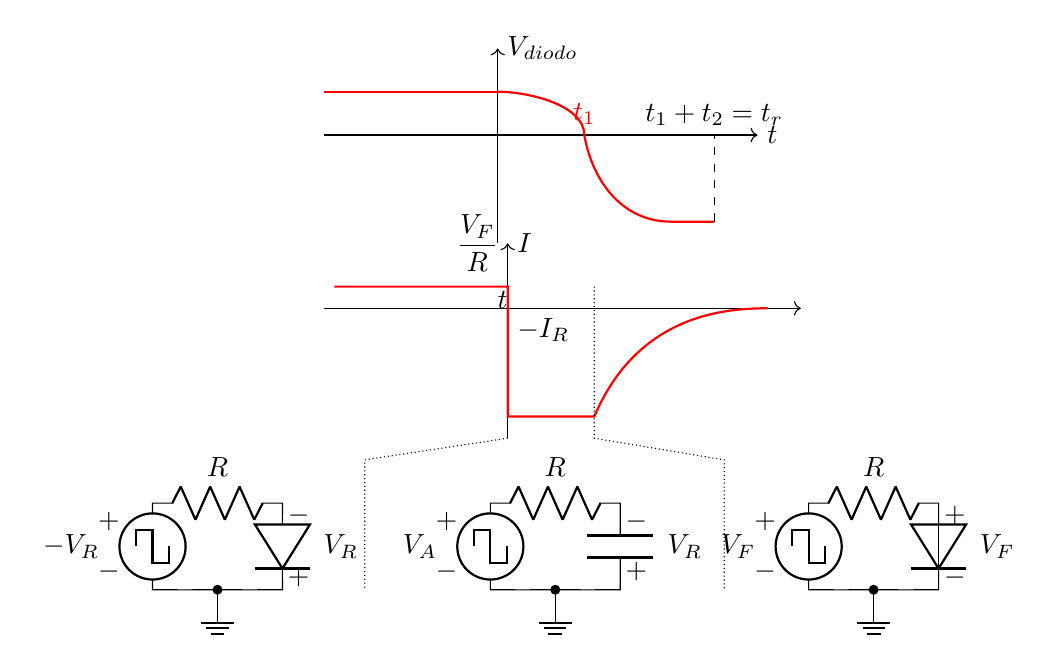
\begin{tikzpicture}[scale=0.55]
    %disegno grafico tensione
        %disegno asse x
        \draw[->] (-4,0+4) node[anchor=north]{}-- (6,0+4)
        node[anchor=west]{$t$};
        %disegno asse y
        \draw[->] (0,-2.5+4)-- (0,2+4) node[anchor= west]{$V_{diodo}$};
        %disegno grafico rosso
        \draw[thick,red] (-4,1+4)-- (0,1+4); 
        \draw[thick,red] (0,1+4) to [out=0, in=90,distance=0.7cm] (2,4) node[above]{$t_1$} ;
        \draw[thick,red] (2,0+4) to [out=280, in=180] (4,-2+4)--++ (1,0);
        %label tempo
        \draw[dashed] (5,2)-- (5,4) node[above]{$t_1+t_2=t_r$};
       %disegno grafico corrente
        %disegno asse x
        \draw[->] (-4,0) node[anchor=north]{}--++ (11,0);
        node[anchor=west]{$t$};
        %disegno asse y
        \draw[->] (0,-3)-- (0,1.5) node[anchor= west]{$I$};
        %disegno grafico rosso
        \draw[thick,red] (-4,0.5)-- (0,0.5) --++ (0,-3)--++ (2,0)
       ..controls (2+1,-0.15) and (4+1,-0).. (5+1,-0);

        %disegno aperture per spazio circuiti
        \draw[densely dotted] (0,-3) -- (-3.3,-3.5)--++ (0,-3);
        \draw[densely dotted] (1+1,0.5)--++ (0,-3.5) -- (4+1,-3.5)--++ (0,-3);
        %label
        \node at (0,-0.5) [right]{$-I_R$};
        \node at (0,1.5) [left]{$\dfrac{V_F}{R}$};
        
        %disegno grafico sinistra
        \draw(-6.7,-6.5) coordinate (zero)
        to [short]++ (-1.5,0)
        to [sqV,v<=$-V_R$]++ (0,2)
        to [R, l=$R$] ++ (3,0)
        to [D, v^<=$V_R$]++ (0,-2)
        to [short,-*]++ (-1.5,0)
        node[ground]{}++ (0,-0.1);
        %disegno grafico centrale
        \draw(0.35+0.75,-6.5) coordinate (zero)
        to [short]++ (-1.5,0)
        to [sqV,v<=$V_{A}$]++ (0,2)
        to [R, l=$R$] ++ (3,0)
        to [C, v^<=$V_R$]++ (0,-2)
        to [short,-*]++ (-1.5,0)
        node[ground]{}++ (0,-0.1);
        %disegno grafico denstra
        \draw(7.7+0.75,-6.5) coordinate (zero)
        to [short]++ (-1.5,0)
        to [sqV,v<=$V_F$]++ (0,2)
        to [R, l=$R$] ++ (3,0) coordinate (x)
        to [D, v^=$V_F$]++ (0,-2)
        to [short,-*]++ (-1.5,0)
        node[ground]{}++ (0,-0.1);
        \draw(x) --++ (0,-2);
    \end{tikzpicture}
    \caption{Transitorio ON-OFF del pn dal punto di vista elettronico}
    \label{Transitorio ON_OFF del pn dal punto di vista elettronico}
\end{figure}
Se si trascura la caduta di tensione del diodo in polarizzazione diretta, si ha che la corrente del diodo subito prima della commutazione vale:
\begin{equation}
    I_F \approx \dfrac{V_F}{R}
\end{equation}
Come nel caso precedente,la tensione di giunzione del diodo non può commutare istantaneamente a causa della capacità di giunzione. Quindi per $t=0^+$ $V_j \approx 0$ e quindi:
\begin{equation}
    i(0^+) \approx \dfrac{-V_R}{R} 
\end{equation}
ossia il diodo conduce nella direzione inversa.\\
Negli istanti iniziali della commutazione, il diodo non è ingrado di comportarsi come circuito aperto, bloccando il passaggio della corrente inversa, ma si comporta come un cortocircuito.\\
Il passaggio della corrente inversa è indispensabile per eliminare i portatori in eccesso accumulati nel lato n della giunzione.\\
E' importante notare che la tensione del diodo resta positiva fino a che non si annulla, in $x_n$, la densità in eccesso delle lacune iniettate. Dopo tale istante il diodo comincia ad essere polarizzato inversamente e la corrente si riduce fino al valore asintotico $I_0$.\\
La fase di commutazione si può studiare in due parti
\begin{enumerate}
    \item La fase iniziale da $0^+$ a $t_1$ il diodo lavora a corrente costante pari a $i(0^+) \approx \dfrac{-V_R}{R}=-I_R$
$T_1$ è definito come il tempo necessario a riassorbire l'eccesso di carica.
    \item Nella fase da $t_2$ a $t_1+t_2$ la corrente del diodo si riduce ad un valore considerato trascurabile.
\end{enumerate}
Il tempo $t_1+t_2$ è definito come tempo di recovery ed è il tempo necessario a produrre l'eccesso di portatori in modalità reverse 
\begin{exbox}[approfondimento formule dal libro]
    nell'ipotesi di diodo assimmetrico $p^+n$:
     \begin{center}
         $i=\dfrac{dq_n'}{dt}+\dfrac{q_n'}{\tau_h}$
     \end{center}
    Con $i=I_F$ per $t<0$ ed $i=-I_R$ per $t>0$.\\
    La soluzione valoda per $t<t_1$, si può scrivere come:
    \begin{equation}
        q_n'(t)=\tau_h \left[ -I_R + (I_F+I_R)e^{-t/\tau_h} \right]
    \end{equation}
\end{exbox}
Nel caso delle lacune, supponendo che la carica in eccesso si annulli per $t=t_r$ si trova:
\begin{equation}
    t_r \approx \tau_h \log\left( 1 + \dfrac{I_F}{I_R}\right)
\end{equation}
Dove, per fini pratici si è posto $t_r=t_1+t_2$ mentre $\tau_h$ è il tempo di vita medio delle lacune.\\
Dall'equazione posso capire che aumentando $I_F$ si andrà ad incrementare la quantità di carica che dovrà essere svuotata. Ma a ben pensarci, l'effetto può essere bilanciato da una sufficente $I_R$ ma questo dipende dalle caratteristiche del diodo.\\
I diodi più veloci sono quelli la cui carica per diffusione è piccola, viceversa sono più lenti.\\
L'altro parametro importante è il tempo di vita medio. Per mantenere tempo di vita basso e quindi favorire la ricombinazione, si usano degli elementi (detti) contaminanti nel silicio. Atomi come l'oro creano dei livelli energetici intermedi, cioè trappole energetiche, che in commutazione aumenta il fattore di ricombinazione di elettroni e lacune.

in conclusione:
\begin{enumerate}
    \item il diodo presenta un comportamento praticamente ideale nella fase di TURN-ON
    
    \item il diodo presenta un comportamento NON ideale nella fase di TURN-OFF

    \item i diodi più veloci non hanno grosso accumulo di $Q_{DIFFUSIVA}$  
    
    \item il tempo di ritardo è proporzionalealla vita media dei portatori minoritari e dipende anche dal rapporto delle correnti diretta e inversa subito dopo la commutazione.

    \item la commutazione può essere accellerata aumentando la corrente inversa (e quindi polarizzando con una $V_A$ maggiore) ma soprattutto riducendo il tempo di vita medio dei portatori minoritari.
    Questo può essere ottenuto mediante drogaggio, introducendo livelli energetici intermedi che.....
    in genere si contamina con l'oro
\end{enumerate}
%
\cleardoublepage%
%
\subsubsection{Giunzione a polarizzazione inversa elevata}
Se la giunzione pn è sottoposta ad una polarizzazion inversa elevata, essa non si comporta come nel caso ideale.
Quello che succede è che, ad una certa tensione, il diodo subisce un processo di rottura (\textbf{\emph{BREAKDOWN: $V_{br}$}}) e la corrente aumenta bruscamente.\\
In parole povere, se viene superata la tensione inversa $V_{br}$, il diodo non è più in grado di opporsi al passaggio di corrente e si comporta come cortocircuito.

\begin{center}
    \begin{tikzpicture}[line cap=round, scale =0.85]
		%diseggno asse x
		\draw[->] (-5,0) -- (5,0) node[below] {$V_A$};
        %disegno asse y
		\draw[->] (0,-5) -- (0,5) node[left] {$I$};
		
		% plot per Va positive
		\draw[domain=-3.4:0.75, samples=400, variable=\x, very thick] plot ({0.6*\x+2},{e^(\x*2)});
		\draw[dashed, line width=0.15mm] (2.5,0) node[below] {$V_\text{s}$} --++ (0,4) ;
  
        % plot per Va negative
        \draw(0,0)-- (-0.25,-0.125)--++ (-2.5,0)
        [domain=-7:0.75, samples=400, variable=\x, very thick] plot ({-1*0.2*\x-4},{-e^(\x*2)-0.125});
		\draw[dashed, line width=0.15mm] (-4.1,0) node[] {$V_\text{br}$} --++ (0,-4) ;
	\end{tikzpicture}
\end{center} 

Ci sono tre meccanismi principali che causano la rottura del diodo, ma noi analizziamo sono i primi due:
\begin{enumerate}
    \item Rottura dovuta a moltiplicazione a valanga

    \item Rottura dovuta a effetto tunnel, più conosciuto come "effetto Zener"

    \item Rottura dovuta a perforazione diretta
\end{enumerate}
Gli effetti li studio separatamente ma bisogna sempre ricordare che nei diodi reali il meccanismo di rottura è una combinazione di tutti i meccanismi elencati.
Più avanti si vedrò che i due meccanismi hanno un diverso comportamento in temperatura.

\cleardoublepage%

\subsubsection{Rottura per perforazione diretta}
accade quando la tensione inversa provoca un aumento della regione di svuotamento talmente grande da coprire tutto il semiconduttore fino a toccare le metallizzazioni, a quel punto non c'è più resitenza al passaggio di elettroni da P verso N, anzi, vengono spinti subito dal campo elettrico dello svuotamento che ormai ricopre praticamente tutto il diodo (o la zona drogata maggiormente).

\subsubsection{Effetto Zener (o tunnel)}
%
\begin{ripasso}[RIPASSO PRIMA DI CONTINUARE]
    Nel caso di un semiconduttore di tipo p fortemente drogato, il livello di Fermi si sposterà in modo che si trovi più vicino alla banda di valenza, facilitando il movimento delle lacune e aumentando la conducibilità del materiale.\\
    Nel caso di un semiconduttore di tipo n fortemente drogato, il livello di Fermi si sposterà in modo che si trovi più vicino alla banda di conduzione, facilitando il movimento degli elettroni e aumentando la conducibilità del materiale.\\
    Siccome i due semiconduttori sono messi a contatto, per mantenere l'uniformità  del disegno, succede che le bande del P salgono in alto mentre le bande dell'N scendono provocando un assottigliamento della regione svuotata (vedi figura sotto).
\end{ripasso}
%
 Nei semiconduttori, l'effetto tunnel può verificarsi quando una particella, come un elettrone, attraversa una barriera di potenziale che teoricamente dovrebbe essere troppo alta da permetterlo. Tuttavia, a livello quantistico, esiste una probabilità non nulla che la particella possa attraversare la barriera anche se, dal punto di vista di fisica classica, non ha energia sufficiente.\\
 
Tralasciando però la probabilità quantistica, esiste un'altro caso in cui si verifica tale evento, ovvero quando i semiconduttori sono fortemente drogati al punto da abbassare i livelli di fermi sotto le regioni proibite.
Infatti, nelle giunzioni fortemente drogate la regione di svuotamente può diventare talmente sottile da permettere il passaggio di portatori dalla banda di valenza del SC1 alla banda di conduzione del SC2 attraverso la banda proibita per effetto tunnel.\\

Il flusso di portatori dovuti all'effetto tunnel aumenta con la polarizzazione inversa perchè al crescere della polarizzazione vi sono più stati pieni della banda di valenza affacciati a stati vuoti della banda di conduzione nel lato opposto alla giunzione.

Ricordo che lo spessore della regione di svuotamento vale:
%
\begin{equation}
    x_n= \sqrt{\dfrac{2\epsilon N_{eq}(V_{bi}-V_A)}{N_D^2}}
\end{equation}
%
Se $N_D \uparrow$ allora la regione si stringe molto fino a che non viene perforata (perforazione diretta). In tal caso si verifica una scarica di elettroni che passa dall'altra parte. (le correnti escono dal catodo, costituito dal mezzo drogato n).

\begin{center}
    \begin{circuitikz}[scale=0.55,transform shape]
        %disegno l'unione di due SC
        %mezzo 1
        \draw(0,3) --++ (4,0);
        \draw(0,0) --++ (4,0);
        %mezzo 2
        \draw(7,-1.5) --++ (4,0);
        \draw(7,-4.5) --++ (4,0);
        %intersezione
        \draw[] (4,3)..controls (5.5,3) and (5.5,-1.5).. (7,-1.5);
        \draw[] (4,0)..controls (5.5,0) and (5.5,-4.5).. (7,-4.5);
        % elettroni
        \foreach \pos in {2,3} {
        \node at (0.7+\pos,-0.75) { \tikz\draw[thick,fill=Ecolour]
        circle (0.14cm) (-0.07,0)-- (0.07,0) ;} ;}
        \foreach \pos in {2.5,3.5} {
        \node at (0.7+\pos,-1) { \tikz\draw[thick,fill=Ecolour]
        circle (0.14cm) (-0.07,0)-- (0.07,0) ;} ;}
        %livelli energetici
        \draw[thick,blue] (7,-0.5)--++ (2,0);
        \draw[thick,blue] (7,-1)--++ (2,0);
        %frecce da elettroni a livelli energetici
        \draw[latex-,red] (6.3,-0.45) arc(55:130:1.55);
        \draw[latex-,red] (6.4,-0.65) arc(55:130:1.53);
        %disegno batteria
        \draw(11.5,-3) to [short,*-]++ (1,0)--++ (0,-3)--++ (-7,0);
        \draw(5.5,-6) to [battery1]++ (-1,0);
        \draw(-0.5,1.5) to [short,*-]++ (-1,0)--++ (0,-7.5)--++ (+6,0);
        %label
        \node at (2,3.5) {$p$};
        \node at (9,3.5) {$n$};

        %inserisco circuito zener
        \draw(12,-0.4)--++ (0.5,0);
        \draw(12,-0.5)--++ (0.5,0);
        \draw(12,-0.6)--++ (0.5,0);

        \draw(14,-1.5) 
        to [short]++ (0,2)
        to [zDo]++ (3,0)
        to [short]++ (0,-2)
        to [battery1]++ (-3,0);
        \draw[-latex] (16,1.2)--++ (-1,0);
    \end{circuitikz}
\end{center}

L'effetto di rottura può comportare la distruzione del dispositivo, ma se viene controllato, si può utilizzare nel diodo Zener.\\

\begin{exbox}[ricordo il diodo zener]
%
Il diodo Zener viene utilizzato comé stabilizzatore di tensione nell'intorno della tensione di breakdown e non a caso  è sempre usato in polarizzazione inversa proprio perchè sfrutta il fenomeno di rottura di tipo tunnel.
\begin{center}
    \begin{circuitikz}
        \draw(0,0) node[ground]{} coordinate(gnd);
        \draw(gnd) to [short,*-]++ (-2,0)
                            to [battery2,invert, l=$V_g$]++ (0,1.5) 
                            to [R,l=$R_g$]++ (2,0) coordinate (d)
                            to [short,*-]++ (1,0)
                            to [R,l=$R_{out}$] ++ (0,-1.5)-| (gnd);
         \draw(d) to [zD,invert] (gnd);
    \end{circuitikz}
    \end{center}
    %
Quando la tensione $V_g$ supera la soglia di breakdown dello zener ($V_{br}$)  l'effetto tunner prevale, lo zener diventa praticamente un cortocircuito e fà passare una parte della corrente di $R_g$ verso massa e salvando il carico a cui è collegato.
%
\begin{align*}
    Iout=I_g-I_z
\end{align*}
%
Lo zener ha comunque dei limiti sulla quantità di corrente che può sopportare. \\
Se $I_z$  supera la soglia indicata dal progettista, il dispositivo si rompe. \\
Ulteriori osservazioni sono fatti nel capitolo xx

\end{exbox}

\subsubsection{Effetto valanga}
In presenza di campi elevati, i portatori di carica (che sono mobili) riescono ad acquisire energia sufficiente da provocare la generazione di una coppia elettrone-lacuna dopo una collisione tra atomi e impurità nel reticolo cristallino.

Le coppie elettrone lacuna ed i portatori di carica da cui sono originati vengono nuovamente accelerati dal campo elettrico ed andranno ad urtare atomi del materiale facendoli ionizzare, cioè  producendo ulteriori coppie libere (questo processo è chiamato ionizzazione da impatto) dando vita al fenomeno di moltiplicazione a valanga dei portatori che darà origine ad una forte corrente inversa.

In una giunzione pn vi sono campi intensi solo nella regione di svuotamento e quindi l'effetto valanga potrà verificarsi solo all'interno di questa regione.

\begin{psbox}
Se il campo elettrico non è sufficientemente intenso, la velocità degli elettroni non è sufficiente a mantenere il breakdown a valanga, negli urti gli elettroni sono riassorbiti dagli atomi ed il processo cessa;
\end{psbox}
\begin{figure}[hbt!]
    \centering
    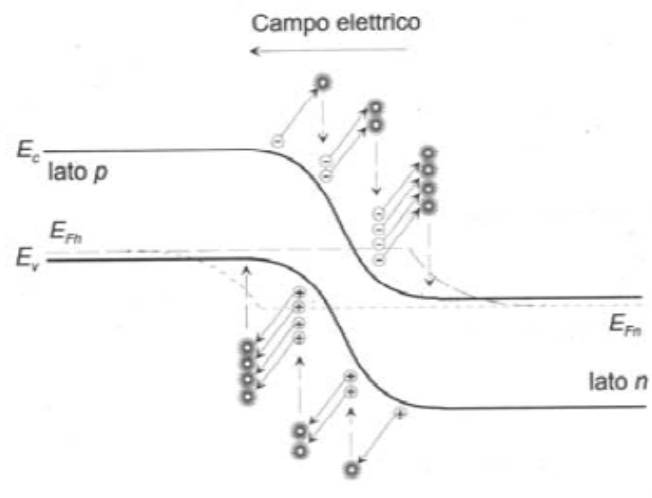
\includegraphics[width=0.5\textwidth]{Immagini_Micro&Nano/Imm_2_Fisica_dei_semiconduttori/Effetto valanga.png}
    \caption{Caption}%
    \label{fig:enter_label}
\end{figure}
%
\textbf{descrizione rigorosa:}\\
La moltiplicazione a valanga di portatori è conseguenza tipica 
 della presenza di un elevato campo elettrico. Infatti, maggiore è il campo, maggiore è la probabilità che si verichi la ionizzazione da impatto e quindi l'effetto valanga, con il conseguente aumento della corrente di trascinamento.\\
Considero un sistema monodimensionale e stazionario nel tempo: un semiconduttore di lunghezza W sottoposto ad un campo elettrico $\mathcal{E}$ (non necessariamente costante lungo x) e quindi percorso da una corrente totale di elettroni $J_n$ e di lacune $J_h$.\\
%
Suppongo  inoltre che il campo sia intenso a tal punto da rendere dominante il fenomeno di generazione per ionizzazione da impatto rispetto ad altri meccanismi, allora scrivo l'equazione di continuità in condizioni stazionarie:

\begin{align}
    \dfrac{dJ_n}{dx}&=-\alpha_h \cdot J_h - \alpha_n \cdot J_n\\
    \dfrac{dJ_h}{dx}&=\alpha_h \cdot J_h + \alpha_n \cdot J_n
\end{align}
dove $\alpha_n$ ed $\alpha_h$ sono i coefficienti di ionizzazione di elettroni e lacune; $\alpha_n$ determina quante coppie elettrone-lacuna vengono generate a causa della della distribuzione $J_n$.  analogo per $\alpha_h$.\\
%
Io sò che la corrente $J^{tot} = J_n(x) + J_h(x)$ è costante lungo $x$ perchè la corrente è uguale sezione per sezione. riscrivo l'equazione EDO nell'incognita $J_h$ usando la  $J^{tot}$ precendente ed ottengo:
%
\begin{equation}
    \dfrac{dJ_h}{dx}=\alpha_h \cdot J_h + \alpha_n \cdot (J-J_h)
\end{equation}
%
Per risolvere questa EDO mi serviranno le condizioni al contorno.
Supponiamo che il campo elettrico sia tale da rendere $J_h$ e $J_n$ positive nelle equazioni di continuità sopra scritte, allora la derivata di $J_h$ rispetto ad x è positiva, ossia $J_h$ cresce progressivamente da x=0 a x=W, 
ricordo però che $J_n=J^{tot}-J_h$ quindi, la densità di corrente di elettroni decresce per x crescenti ( analogamente cresce per x decrescenti). Questo corrsiponde al fatto che le lacune si muovano da sinistra verso destra, generando coppie elett-lacuna, mentre gli elettroni si muovono nel verso opposto.\\
%
\begin{figure}[hbt!]
    \centering
    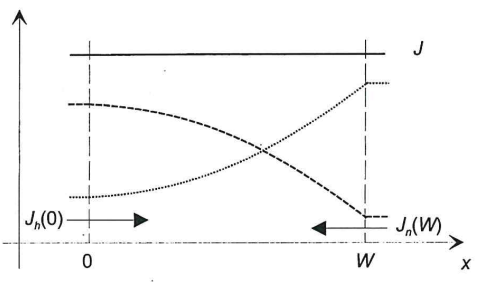
\includegraphics{Immagini_Micro&Nano/Imm_2_Fisica_dei_semiconduttori/condizioni al contorno per generazione a valanga.png}
    \caption{Caption}%
    \label{fig:enter_label}
\end{figure}
%
Per le condizioni al contorno posso, allora considera una corrente di lacune $J_h(0)$ incidente da sinistra ed una corrente di elettroni $J_n(0)$ incidente da destra. Questa considerazione non è tirata a caso infatti, posso considerarla coerente con il processo di generazione a valanga delle lacune che origina in x=0 e prosegue verso sinistra, mentre il processo per gli elettroni ha origine in x=W e procede verso destra.

La soluzione finale sarà:
%
\begin{equation*}
    J=\dfrac{\exp{\left[ \alpha_h - \alpha_n\right]_{0}^{W}} J_h(0)+J_n(W)}{\exp{\left[ \int_{0}^{W} \alpha_h - \alpha_n dx \right] \int_{0}^{W} \alpha_n \cdot \exp{\left[ -\int_{0}^{\xi} \alpha_h \alpha_n d\xi\right] dx}}}
\end{equation*}
%
l'equazione risolutiva $J$ è un qualcosa di molto complicato che non studio, tuttavia è molto importante sapere che \textbf{in presenza di una finita corrente iniettata di elettroni e lacune, la corrente totale $J$ può diventare infinita (o grande) grazie al venomeno di generazione elettrone-lacuna}.\\

A me interessa il caso particolare in cui $J \rightarrow \infty$ e questo succede solo se:
\begin{equation*}
    \int_{0}^{W}\alpha_h \exp{\left[ -\int_{0}^{x} (\alpha_h - \alpha_n) d\xi \right] dx} =1
\end{equation*}
%
l'equazione precedente è chiamata integrale di ionizzazione.\\
Per non complicare la trattazione supponiamo valide due ipotesi 
semplificative:
 \begin{enumerate}
     \item la giunzione è brusca asimmetrica ($p^+n$)
     \item I coefficienti di ionizzazione di elettroni e lacune sono uguali, ossia $\alpha_n=\alpha_h=\alpha$
 \end{enumerate}
L'integrale diventa semplice nel caso in cui si applichi la condizione semplificativa num.2.  Allora la condizione di rottura per effetto valanga diventa:
\begin{equation}
    \int_{0}^{W}\alpha_h dx = \int_{0}^{W}\alpha_n dx = 1 
\end{equation}

La condizione $\alpha_h \approx \alpha_n$ è verificata nel GaAs ed in altri semiconduttori ma non è vera nel silicio. in quest'ultimo, i due tassi di ionizzazione sono molto differenti e la condizione di valanga si ottiene per tensioni molto maggiori siccome uno dei due portatori dovrà compensare la minore efficienza di ionizzazione dell'altro.\\
%
Sia $\alpha_n$ che $\alpha_h$ sono funzioni del campo elettrico, quindi 
\begin{equation}
    \alpha_n = \alpha_h=\alpha^{\infty} \exp\left[ -\dfrac{\mathcal{E}^{crit}}{\mathcal{E}} \right]
\end{equation}

Se il campo $\mathcal{E}$ è è molto debole allora $\alpha_n=\alpha_h=0$ quindi l'integrale sopra farà 0 e la condizione "$=1$" non è mai soddisfatta.\\
Se il campo $\mathcal{E}$ è molto grande allora $\alpha_n=\alpha_h=\alpha^{\infty}$ \\
in tutte le altre condizioni, siccome il campo elettrico cambia all'interno della regione svuotata,  allora $\alpha_n$ ed $\alpha_h$ avranno certi andamenti (che noi non vediamo) e se capito che $\int_{0}^{\infty}\cdot=1$ allora si sviluppa quella corrente.\\
ricordo che il campo elettrico è pari a 
\begin{equation}
    \mathcal{E}=\mathcal{E}_{max}\ \exp\left[\dfrac{x-x_n}{x_n}\right]
\end{equation}
\textbf{CONTROLLARE FORMULA SE CORRETTA}\\
\cleardoublepage%
In definitiva ci sono due casi in cui si può verificare uno scorrere della corrente:
\begin{itemize}
    \item nel caso di effetto tunnel. nel quale c'è bisogno di un elevato drogaggio
    \item nel caso di effetto valanga nel quale c'è bisogno di un drogaggio sufficiente ma tanta $V_A$.
\end{itemize}
%
Definisco ora la tensione di breackdown in funzione del drogaggio:\\
\begin{figure}[hbt!]
    \centering
    \begin{tikzpicture}
        %disegno asse x e label
        \draw[-latex] (0,0)-- (6,0) node [right]{$\text{Drogaggio lato n }(cm^{-3}$};
        \node at (0.25,0)[below]{$10^4$};
        \node at (5.5,0)[below]{$10^{18}$};
        %disegno asse y
        \draw[-latex] (0,0)-- (0,4) node [right]{$V_{BD}$};
        \node at (0,0)[left]{$1$};
        \node at (0,1)[left]{$10$};
        \node at (0,2)[left]{$100$};
        \node at (0,3)[left]{$10$kV};
        %disegno grafico
        \draw[] (0,3.25) to [out=300,in=180] (5.5,0.55);
    \end{tikzpicture}
    \caption{Caption}%
    \label{fig:enter_label}
\end{figure}
\\%
Dalla figura vediamo i valori in gioco per quanto riguarda al tensione di breakdown. per drogaggi bassi la tensione aumenta. mentre per drogaggi alti la tensione si abbassa (quindi la scarica avviene prima).

\subsubsection{Dipendenza dalla temperatura}
Da un altro punto di vista più applicativo possiamo vedere la dipendenza dei due fenomeni al variare della temperatura.

\begin{figure}[hbt!]
\centering
    \begin{subfigure}{0.49\textwidth}
        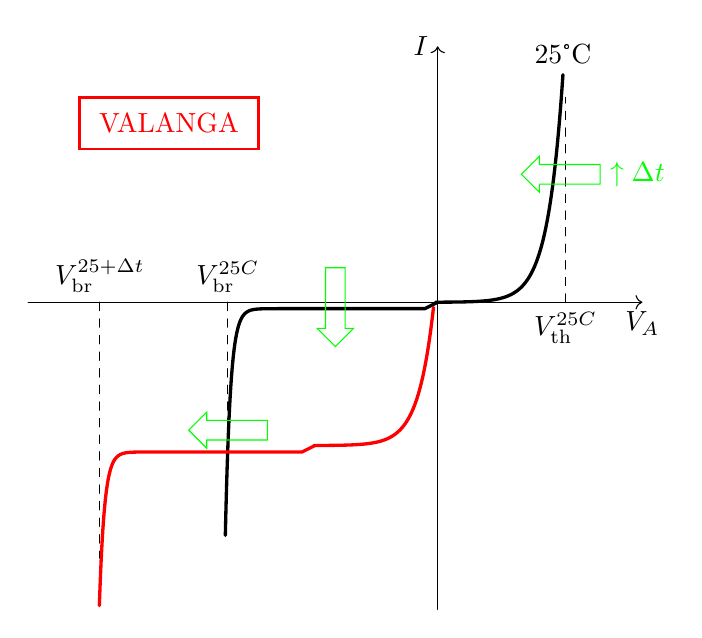
\begin{tikzpicture}[line cap=round,scale=0.65]
		%diseggno asse x
		\draw[->] (-8,0) -- (4,0) node[below] {$V_A$};
        %disegno asse y
		\draw[->] (0,-6) -- (0,5) node[left] {$I$};
		
		% plot per Va positive
		\draw[domain=-3.4:0.75, samples=400, variable=\x, very thick] plot ({0.6*\x+2},{e^(\x*2)}) node[above]{25°C};
      %label soglia
		\draw[dashed, line width=0.15mm] (2.5,0) node[below] {$V_\text{th}^{25°C}$} --++ (0,4) ;
        % plot per Va negative
        \draw(0,0)-- (-0.25,-0.125)--++ (-2.5,0)
        [domain=-7:0.75, samples=400, variable=\x, very thick] plot ({-1*0.2*\x-4},{-e^(\x*2)-0.125});
          %tensione breakdown
		\draw[dashed, line width=0.15mm] (-4.1,0) node[anchor=south] {$V_\text{br}^{25°C}$} --++ (0,-3) ;

        %plot rosso traslato
        \draw[domain=-3.4:0.5, samples=400, variable=\x, very thick,red] plot ({0.6*\x-0.38},{e^(\x*2)-2.8});
         \draw(-2.4,-2.8)-- (-2.65,-2.925)--++ (-2.5,0)
        [domain=-7:0.55, samples=400, variable=\x, very thick,red] plot ({-1*0.2*\x-6.5},{-e^(\x*2)-2.925});
       % disegno frecce temepratura
         %freccia in T
  \node at (2.5,2.5)[single arrow, draw=green,
      minimum width = 10pt, single arrow head extend=3pt,
      minimum height=10mm,rotate=180] {}; % length of arrow
       \node at (3,2.5) [right,green]{$\ \uparrow\Delta t$};
  \node at (-4,-2.5)[single arrow, draw=green,
      minimum width = 10pt, single arrow head extend=3pt,
      minimum height=10mm,rotate=180] {}; % length of arrow
      \node at (-2,-0)[single arrow, draw=green,
      minimum width = 10pt, single arrow head extend=3pt,
      minimum height=10mm,rotate=-90] {}; % length of arrow
        %label rosso 
        \draw[dashed, line width=0.15mm] (-6.6,0) node[anchor=south] {$V_\text{br}^{25°+\Delta t}$} --++ (0,-5) ;

        %scritta rossa
        \draw[thick, red] (-7,3) rectangle++ (3.5,1) node[pos=.5, red] {VALANGA};
	\end{tikzpicture}
\caption{Caption}%
\label{fig:enter_label}
\end{subfigure}
\begin{subfigure}{0.49\textwidth}
    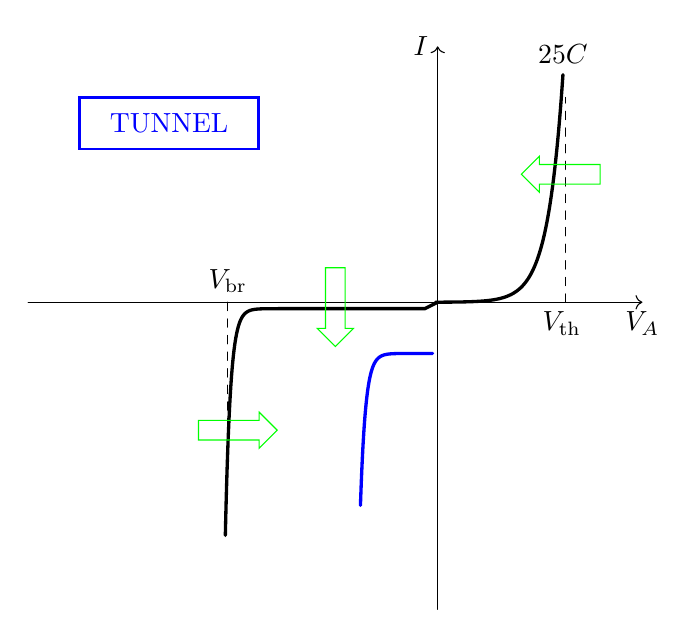
\begin{tikzpicture}[line cap=round,scale=0.65]
		%diseggno asse x
		\draw[->] (-8,0) -- (4,0) node[below] {$V_A$};
        %disegno asse y
		\draw[->] (0,-6) -- (0,5) node[left] {$I$};
		
		% plot per Va positive
		\draw[domain=-3.4:0.75, samples=400, variable=\x, very thick] plot ({0.6*\x+2},{e^(\x*2)}) node[above]{$25°C$};
		\draw[dashed, line width=0.15mm] (2.5,0) node[below] {$V_\text{th
  }$} --++ (0,4) ;
        % plot per Va negative
        \draw(0,0)-- (-0.25,-0.125)--++ (-2.5,0)
        [domain=-7:0.75, samples=400, variable=\x, very thick] plot ({-1*0.2*\x-4},{-e^(\x*2)-0.125});
		\draw[dashed, line width=0.15mm] (-4.1,0) node[anchor=south] {$V_\text{br}$} --++ (0,-3) ;

        %plot blu traslato
         \draw[domain=-6.5:0.55, samples=400, variable=\x, very thick,blue] plot ({-1*0.2*\x-1.4},{-e^(\x*2)-1});
         %freccia in T
  \node at (2.5,2.5)[single arrow, draw=green,
      minimum width = 10pt, single arrow head extend=3pt,
      minimum height=10mm,rotate=180] {}; % length of arrow
    \node at (-2,0)[single arrow, draw=green,
      minimum width = 10pt, single arrow head extend=3pt,
      minimum height=10mm,rotate=-90] {}; % length of arrow
  \node at (-4,-2.5)[single arrow, draw=green,
      minimum width = 10pt, single arrow head extend=3pt,
      minimum height=10mm,rotate=0] {}; % length of arrow
        

        %scritta rossa
        \draw[thick, blue] (-7,3) rectangle++ (3.5,1) node[pos=.5, blue] {TUNNEL};
	\end{tikzpicture}
    \caption{Caption}%
    \label{fig:enter_label}
\end{subfigure}

    \caption{Caption}%
    \label{fig:enter_label}
\end{figure}
\cleardoublepage%
\paragraph{Dipendenza dalla temperatura dell'effetto valanga}\mbox{}\\
Se io alzo la temperatura, la curva si sposta a sinistra indicando una diminuzione della tensione di soglia $V_{th}$. Questo è legato al fatto che se T sale allora ci sono più elettroni in banda di conduzione (perchè $n_i^2 \uparrow)$ e quindi ci sarà maggior probabilità che la giunzione vada ON.
L'aumento della temperatura si porta dietro altri due fenomeni:
\begin{itemize}
    \item Aumento della corrente inversa di saturazione: dovuto dal fatto che la probabilità di generazione spontanea di coppie elettrone-lacuna aumenta a causa dell'energia termica aggiuntiva. Questo comporta un aumento della densità di portatori di carica minoritaria liberi e, di conseguenza, un aumento della corrente inversa attraverso la giunzione. 
    \item Aumento della tensione di breakdown nel processo di moltiplicazione a valanga: L'effetto valanga è amplificato a temperature più elevate. Le vibrazioni atomiche associate all'aumento della temperatura forniscono un meccanismo aggiuntivo per l'accelerazione dei portatori di carica, aumentando quindi la probabilità di ionizzazione a valanga. Di conseguenza, la tensione di breakdown nel processo di moltiplicazione a valanga diminuisce a  temperature più elevate (lacurva si sposta verso sinistra).
\end{itemize}se ho a che fare con una temperatura più alta ($t+\Delta t$), osservo che ho tanta più corrente inversa di saturazione e anche maggior tensione di breakdown nel processo di moltiplicazione a valanga. Ciò è legato a meccanismi vibrazionaliche dissipano l'energia acquisita
%
\begin{ricevimento}
    manca un pezo illeggibile:
    c'è bisogno di più campo per generare coppie elettroni perchè.. d più lungo
\end{ricevimento}
%
\paragraph{Dipendenza dalla temperatura dell'effetto zener}\mbox{}\\
Il meccanismo dell'effetto zener è leggermente diverso:
L'effetto zener si verifica quando il camp elettrico è sufficientemente forte da aumentare la mobilità degli elettroni in banda di valenza, permettendogli di superare l'energy gap ed entrare nella banda di conduzione. 
Siccome l'aumentare della temperatura consente agli elettroni di acquisire maggiore energia cinetica la quantità di campo elettrico ulteriore, necessaria agli elettroni per andare in banda di conduzione, diminuisce e di conseguenza diminuirà anche la tensione richiesta (tensione e campo elettrico sono relazionati). 
\begin{ricevimento}
    dicono tutti che pet T che aumenta il gap energetico diminuisce.. ma non credo sia giusto. almeno non vedo il nesso. forse intendono che gli elettroni che passano aumentano della stessa quantità uguale a quella che arei considerando il caso standard ma con energy gap minore.
\end{ricevimento}
In parole povere, l'effetto breakdown zener è un comportamento con coefficente negativo in temperatura.
\\
La perdia di efficienza nel meccanismo VALANGA diventa vantaggioso nel meccanismo TUNNEL perchè gli elettroni hanno più energia e riescono ad attraversare la barriera con meno campo elettrico . nello zener la temperatura c'entra poco perchè dipende tutto dai livelli energetici: l'abbassamento di 2 ed 1 non è del tutto dimostrabile da Shotkcley.
In generale si può dire che l'effetto zener avviene prima dell'effetto valanga. Si nota che per entrambi gli effetti si ha un aumento di $I_R$ all'aumentare della temperatura.\\
Questo può esssere spiegato dalla relazione di shotckley:
\begin{equation}
    J=\underbrace{q\ n_i^2 \left[ \dfrac{D_n}{N_A\ L_n} + \dfrac{D_p}{N_D\ L_p}\right]}_{I_0} \cdot \left[\exp{\dfrac{V_A}{V_T}-1}\right]
\end{equation}
c'è un'altra equazione intravista, quella della corrente inversa:
\begin{equation}
    J_R= \underbrace{\dfrac{q\ n_i^2\ W(V_A)}{\tau_n\ \tau_p}}_{J_{SC}} \cdot \left[\exp{\dfrac{V_A}{2V_T}-1}\right]
\end{equation}
$J_{SC}$ (aumenta proporzionalmente con $V_A$)è responsabile del trattino in basso ed è molto maggiore di $J_0$
\begin{figure}[hbt!]
    \centering
    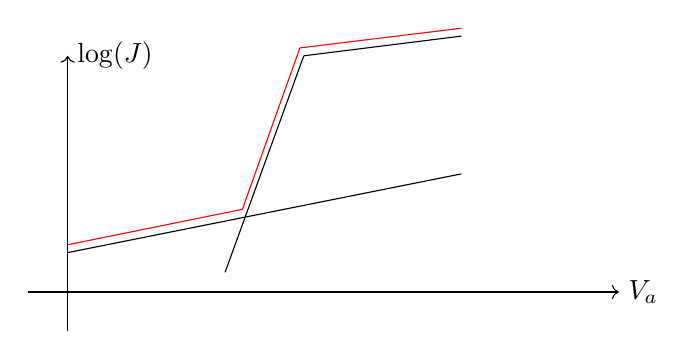
\begin{tikzpicture}
        % disegno asse x
        \draw[->] (-0.5,0)-- (7,0) node[right]{$V_a$};
        % disegno asse y
        \draw[->] (0,-0.5)-- (0,3) node[right]{$\log(J)$};
        %disegno J_SC
        \draw[] (0,0.5)-- (5,1.5);
        %disegno J_0
        \draw[] (2,0.25)-- (3,3);
        %disegno R_serie
        \draw[] (3,3)-- (5,3.25);
        %grafico rosso
        \draw[red] (0,0.6)-- (2.22,1.05)-- (2.95,3.1)-- (5,3.35);
    \end{tikzpicture}
    \caption{Caption}%
    \label{fig:enter_label}
\end{figure}



   \cleardoublepage%
\subsection{GIUNZIONE METALLO-SEMICONDUTTORE: il diodo Schottky}
la giunzione emetallo-semiconduttore è un'eterogiunzione; pertanto è conveniente descrivere il potenziale elettrostatico in funzione del livello del vuoto.\\
Detta $E_w^M$ la funzione lavoro del metallo e $E_w^S$ la funzione lavoro del semiconduttore, si possono verificare quattro casi con i corrispettivi comportamenti elettrici:\\

\noindent\begin{minipage}{0.55\textwidth}
\begin{equation}
    \text{semiconduttore: } n \begin{cases}
    E_w^M > E_w^S & \text{giunzione raddrizzante }\\\\
    E_w^M < E_w^S & \text{giunzione ohmica }
\end{cases}
\end{equation}\\
\begin{equation}
    \text{semiconduttore: } p \begin{cases}
    E_w^M < E_w^S & \text{giunzione raddrizzante }\\\\
    E_w^M > E_w^S & \text{giunzione ohmica }
\end{cases}
\end{equation}
\end{minipage}%
\hfill%
\begin{minipage}{0.3\textwidth}
    \centering
    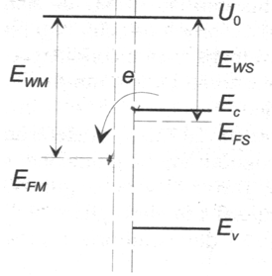
\includegraphics[width=\textwidth]{Immagini_Micro&Nano/Imm_2_Fisica_dei_semiconduttori/giunzione MeSC.PNG}
    \captionof{figure}{caption}
    \label{fig:enter_label}
\end{minipage}

\subsubsection{Semiconduttore di tipo n:}
la prima figura mostra le bande (e quindi i livelli energetici) del metallo e semiconduttore poco prima del contatto.\\
\begin{figure}[hbt!]
    \centering
    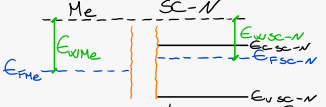
\includegraphics{Immagini_Micro&Nano/Imm_2_Fisica_dei_semiconduttori/giunzioneMeSCn.PNG}
    \caption{Caption}%
    \label{fig:enter_label}
\end{figure}
Al contatto, visto che $E_{wSCn} < E_{wM}$, gli elettroni del semiconduttore tendono a passare nel metallo, dove il livello di fermi è appunto inferiore.
\begin{center}
    \begin{circuitikz}
        %livello fermi metallo
        \draw[dashed] (0,0)--++ (4,0);
        %livello fermi SC
        \draw[dashed] (4,0)--++ (4,0);
        %disegno banda SC
        \draw[domain=0:3.3, samples=400, variable=\x, very thick] plot ({1.2*\x+4},{e^(-1*\x)+0.1});
        \draw[domain=0:3.3, samples=400, variable=\x, very thick] plot ({1.2*\x+4},{e^(-1*\x)-1.9});
        %tratteggi
        \draw[densely dashed] (4,1.1)--++ (0,-3.1);
        \draw[densely dashed] (4,1.1)--++ (4,0);
        %doppie freccie e label
        \draw[>=latex, <->] (6.3,0.25)-- (6.3,1.1);
        \node at (6.3,0.65) [right]{$qV_{bi}$};
        %----
        \draw[>=latex, <->] (3.9,0)-- (3.9,1.1);
        \node at (3.9,0.55) [left]{$q\phi_{Bn}$};
        %----
        \node at (1.7,1.5) []{Metallo};
        \node at (6,1.5) []{SC};
        
        %inserisco elettrone e freccia
        \node at (5,0.8) { \tikz\draw[thick,fill=Ecolour]
        circle (0.13cm) (-0.08,0)-- (0.08,0) ;};
         \node at (4.5,0.9) { \tikz\draw[thick,fill=Ecolour]
        circle (0.13cm) (-0.08,0)-- (0.08,0) ;};
         \node at (5.5,0.6) { \tikz\draw[thick,fill=Ecolour]
        circle (0.13cm) (-0.08,0)-- (0.08,0) ;};

        \draw[-latex] (4.5,1) arc(40:165:1);
        %disegno diodo
        \draw(3,2.5) to [sDo]++ (2,0);
        \node at (3.94,1.85) []{$|||$};
    \end{circuitikz}
\end{center}
La superficie del semiconduttore si svuota dei portatori, mentre nel metallo si forma una regione superficiciale carica negativamente, il cui spessore è trascurabile rispetto alla regione di svuotamento del semiconduttore: La carica sul metallo è virtualmente superficiale.

%
-------------------------------------------------------------\\
Supponiamo di trascurare la corrente dei portatori minoritari. Allora possiamo dire che la condizione di equilibrio termodinamicosi stabilisce quando la corrente totale che attraversa la giunzion è nulla.\\
Questa corrente (costituita quasi totalmente da portatori maggioritari, cioè elettroni) può essere scomposta in due contributi uguali ed opposti:
Corrente associata al flusso di elettroni che vanno dal metallo al semiconduttore e corrente associata al flusso di elettroni che vanno dal semiconduttore al metallo.

Indichiamo con $J_{SM}$ la densità di correntee legata ai portatori che vanno dal semiconduttore al metallo e $J_{MS}$ la densità di corrente legata ai portatori che vanno dal metallo al semiconduttore.
In condizione di equilibrio termodinamico non fluisce corrente, ossia $J_{SM0}=J_{MS0}$.\\
-------------------------------------------------------------\\
Come nel caso di giunzione tra semiconduttori, anche in questo caso si creerà un campo elettrico; il potenziale $\phi$ si può trovare come integrale del campo elettrico lungo x e l'andamento dell'energia si può trovare come $-q\phi$.
A seguito dell'unione dei due mezzi, ai capi della giunzione is forma un potenziale di built-in:
\begin{equation}
    qB_{bi}=E_W^M-E_W^S
\end{equation}
Inltre, all'equilibrio, mentre sul semiconduttore n si sarà instaurata una regione di svuotamento, gli elettroni saranno confinati del metallo a causa di una barriera di potenziale $q\phi_{Bn}=E_W^M-q\alpha$
(dove $\alpha$ è l'affinità elettronica del semiconduttore).\\
\subsubsection{Polarizzazione diretta: $V_A >0$}
per $Va>0$
\begin{center}
    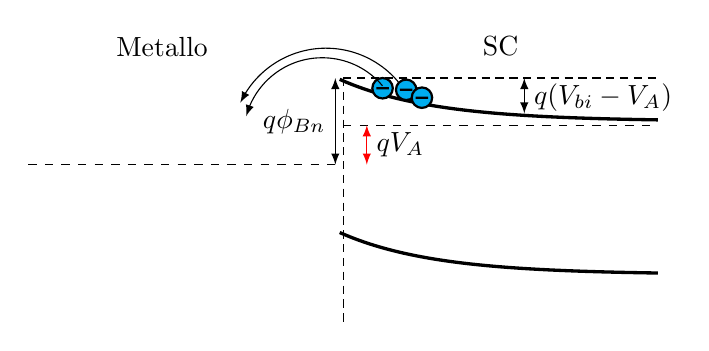
\begin{tikzpicture}
        %livello fermi metallo
        \draw[dashed] (0,0)--++ (4,0);
        %livello fermi SC
        \draw[dashed] (4,0.5)--++ (4,0);
        %disegno banda SC
        \draw[domain=0.63:4, samples=400, variable=\x, very thick] plot ({1.2*\x+3.2},{e^(-1*\x)+0.55});
        \draw[domain=0.63:4, samples=400, variable=\x, very thick] plot ({1.2*\x+3.2},{e^(-1*\x)-1.395});
        
        %tratteggi
        \draw[densely dashed] (4,1.1)--++ (0,-3.1);
        \draw[densely dashed] (4,1.1)--++ (4,0);
        %doppie freccie e label
        \draw[>=latex, <->, red] (4.3,0)--++ (0,0.5);
        \node at (4.3,0.25) [right]{$qV_{A}$};
        %----
        \draw[>=latex, <->] (3.9,0)-- (3.9,1.1);
        \node at (3.9,0.55) [left]{$q\phi_{Bn}$};
        %----
        \draw[>=latex, <->] (6.3,0.65)-- (6.3,1.1);
        \node at (6.3,0.85) [right]{$q(V_{bi}-V_{A})$};
        %----
        \node at (1.7,1.5) []{Metallo};
        \node at (6,1.5) []{SC};
        
        %inserisco elettrone e freccia
        \node at (4.5,0.97) { \tikz\draw[thick,fill=Ecolour]
        circle (0.13cm) (-0.08,0)-- (0.08,0) ;};
        \node at (4.8,0.95) { \tikz\draw[thick,fill=Ecolour]
        circle (0.13cm) (-0.08,0)-- (0.08,0) ;};
         \node at (5,0.85) { \tikz\draw[thick,fill=Ecolour]
        circle (0.13cm) (-0.08,0)-- (0.08,0) ;};

         \draw[-latex] (4.5,1) arc(40:165:1);
         \draw[-latex] (4.7,1.05) arc(40:155:1.2);
    \end{tikzpicture}
\end{center}
Polarizzando direttamente la barriera di potenziale si abbassa. la corrente di diffusione degli elettroni $J_{SM}$ non è più compensata dall'opposta corrente di deriva($J_{SM}>J_{SM0}$.) ma $J_{SM0}=J_{MS0}=J_{MS}$, pertanto $J_{SM0}>J_{MS0}$ e la giunzione conduce corrente dipendente in modo esponenziale dalla tensione applicata (similmente alla giunzione pn).


\subsubsection{Polarizzazione inversa: $V_A <0$}
per $Va<0$
\begin{center}
    \begin{tikzpicture}
        %livello fermi metallo
        \draw[dashed] (0,0)--++ (4,0);
        %livello fermi SC
        \draw[dashed] (4,-0.5)--++ (4,0);
        
        %disegno banda SC
        \draw[domain=0:4.5, samples=400, variable=\x, very thick] plot ({0.9*\x+4},{1.55*e^(-1.05*\x)-0.45});
        \draw[domain=0:4.5, samples=400, variable=\x, very thick] plot ({0.9*\x+4},{1.55*e^(-1.05*\x)-2.295});
        
        %tratteggi
        \draw[densely dashed] (4,1.1)--++ (0,-3.5);
        \draw[densely dashed] (4,1.1)--++ (4,0);
        
        %doppie freccie e label
        \draw[>=latex, <->, red] (3.9,0)--++ (0,-0.5);
        \node at (4,-0.25) [left]{$qV_{A}$};
        %----
        \draw[>=latex, <->] (3.9,0)-- (3.9,1.1);
        \node at (3.9,0.55) [left]{$q\phi_{Bn}$};
        %----
        \draw[>=latex, <->] (6.3,-0.38)-- (6.3,1.1);
        \node at (6.3,0.35) [right]{$q(V_{bi}-V_{A})$};
        %----
        \node at (1.7,1.5) []{Metallo};
        \node at (6,1.5) []{SC};
        
        %inserisco elettrone
        \node at (5.3,0.1) { \tikz\draw[thick,fill=Ecolour]
        circle (0.13cm) (-0.08,0)-- (0.08,0) ;};
        \node at (5.6,0) { \tikz\draw[thick,fill=Ecolour]
        circle (0.13cm) (-0.08,0)-- (0.08,0) ;};
         \node at (6,-0.1) { \tikz\draw[thick,fill=Ecolour]
        circle (0.13cm) (-0.08,0)-- (0.08,0) ;};

    \end{tikzpicture}
\end{center}
Polarizzando inversamente, la barriera di potenziale nel lato semiconduttore si innalza e gli elettroni del semiconduttore vengono respinti verso destra.\\
---si forma quindi un flusso di elettroni dal metallo al semiconduttore che è sostenuto, all'interfaccia metallo-SC, NOP pg 366 fondo...


\begin{figure}[hbt!]
    \centering
    \begin{tikzpicture}[scale=0.5]
             %disegno asse x
            \draw[->] (-2,0) node[anchor=north]{}-- (5,0)
            node[anchor=west]{$x$};
            %disegno asse y
            \draw[->] (0,-3.5)-- (0,3) node[anchor=south west]{$\rho_{fissa}(x)$};
            %disegno grafici
            \draw[thick,pattern=north east lines, pattern color=gray] (0,0)rectangle++ (4,2);
            \draw[-latex, line width=0.75mm] (0,0)--++ (0,-3);
            %label
            \node at (4,0) [anchor=north]{$x_n$};
            \node at (0,2) [anchor=east]{$qN_D$};
            \node at (0,-2.5) [anchor=west]{$-qN_A$};
            \node at (2,1) [red]{$Q^+$};

            %disegno grafico energia
            %disegno asse x
            \draw[->] (-2,-5.5) node[anchor=north]{}-- (5,-5.5)
            node[anchor=west]{$x$};
            %disegno asse y
            \draw[->] (0,-9.5)-- (0,-3.7) node[anchor= west]{$\mathcal{E}(x)$};
            %disegno grafico rosso
            \draw[thick,red] (0,-9)-- (4,-5.5)-- (5,-5.5);
            %label
            \node at (0,-9) [anchor=west]{$\mathcal{E}_{MAX}$};

            %disegno grafico potenziale
            %disegno asse x
            \draw[->] (-2,-12.5) node[anchor=north]{}-- (6,-12.5)
            node[anchor=west]{$x$};
            %disegno asse y
            \draw[->] (0,-15.5)-- (0,-9.7) node[anchor= west]{$\phi(x)$};
            %disegno grafico tensione
            \draw[thick] (0,-12.5).. controls (1.5,-12.5) and (1,-10.7) .. (4,-10.5)--++ (1,0) node[anchor=west]{$V_{bi}$};;
            %disegno grafico potenziale
            \draw[thick] (0,-12.5).. controls (1.5,-12.5) and (1,-15.7) .. (4,-15.5)--++ (1,0);
            \draw[<->] (4,-15.5)-- (4,-12.5);
            \node at (4,-14)[anchor=west]{$q(V_{bi}-V_A)$};
            %label
            \node at (0,-11) [anchor=west]{$\mathcal{E}_{MAX}$};
    \end{tikzpicture}
    \caption{Caption}%
    \label{fig:enter_label}
\end{figure}






manca una figura...\\
\cleardoublepage%
\paragraph{caso giunzione ohmica SCn-Me: $E_w^{Me} > E_w^{SC}$}
%
\begin{figure}[hbt!]
    \centering
    \begin{subfigure}{0.5\textwidth}
        \centering
            \begin{tikzpicture}
            %disegno livello virtuale
            \draw(0,0)--++ (6.5,0);
            %disegno livello fermi per il metallo
            \draw[dashed] (0,-2)--++ (3,0);
            %disegno Banda e fermi del SC
            \draw[] (3,-2.5)--++ (3,0);
            \draw[dashed] (3,-3)--++ (3,0);
            \draw[] (3,-4.5)--++ (3,0);
    
            %livello eergetico metallo
            \draw[>=latex, <->] (1.5,0)--++ (0,-2);
            \node at (1.5,-1) [right]{$E_W^M$};
            %livello energetico SC
            \draw[>=latex, <->] (4.5,0)--++ (0,-3);
            \node at (4.5,-1) [right]{$E_W^S$};
    
            %inserisco elettrone e freccia
            \foreach \pos in {0,0.35}{
            \node at (2.5+ \pos,-1.8) { \tikz\draw[thick,fill=Ecolour]
            circle (0.13cm) (-0.08,0)-- (0.08,0) ;};}
             
             \draw[latex-] (3.5,-2.35) arc(0:75:0.5);
        \end{tikzpicture}
        \caption{Caption}%
        \label{fig:enter_label}\par\vfill
        \end{subfigure}
        %
        \begin{subfigure}{0.5\textwidth}
        \centering
            \begin{tikzpicture}[scale=1]
            %disegno asse x
            \draw[-latex] (-3,0)-- (3,0) node[right]{x};
           % \draw[white]{}(3,0)--++ (0.5,0);
            %disegno asse y
            \draw[-latex] (0,-2)-- (0,2) node[left]{$\rho$};
            %disegno rosso
            \draw[-latex,red,very thick] (0,0)--++ (0,1);
            %disegno blu
        \end{tikzpicture}
        \caption{Caption}%
        \label{fig:enter_label}\par\vfill
        \end{subfigure}
        %
        \begin{subfigure}{0.5\textwidth}
        \centering
            \begin{tikzpicture}
            %disegno asse x
            \draw[dashed] (-3,0)-- (3,0) node[right]{$E_F$};
            %disegno asse y
            \draw[densely dashed] (0,-2)-- (0,2);
            %disegno banda C
            \draw[very thick] (0,-0.4) to [out=60, in=180] (1.5,0.35)--++ (1,0) node[right]{$E_C$};
            %disegno banda V
            \draw[very thick] (0,-1.4) to [out=60, in=180] (1.5,-0.65)--++ (1,0) node[right]{$E_V$};
        \end{tikzpicture}
        \caption{Caption}%
        \label{fig:enter_label}
        \end{subfigure}
        \begin{subfigure}{0.5\textwidth}
        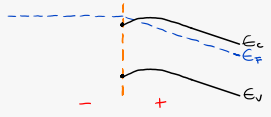
\includegraphics{Immagini_Micro&Nano/Imm_2_Fisica_dei_semiconduttori/giunzione ohmica SCn-Me con Va negativa sul metallo.png}
        \caption{Caption}%
        \label{fig:enter_label}
        \end{subfigure}
        \begin{subfigure}{0.5\textwidth}
        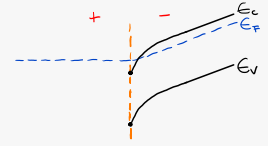
\includegraphics{Immagini_Micro&Nano/Imm_2_Fisica_dei_semiconduttori/giunzione ohmica SCn-Me con Va positiva sul metallo.png}
        \caption{Caption}%
        \label{fig:enter_label}
        \end{subfigure}
\end{figure}
La situazione si analizza come nel caso precedente. Questa volta gli elettroni passeranno dal metallo a semiconduttore.
Questi elettroni si troveranno iniettati in un semicodnuttore in cui sono portatori maggioritari (poi c'è tutto un discorso di debay che non si è spiegato)

non si crea una regione svuotata nè una barriera di potenziale.

Applicando un potenziale positivo al metallo e negativo al semicodnuttore, non essendo presente la regione di svuotamento, si avrà che questo risulta applicato a tutta la giunzione andando a ruotare le bande come nel grafico..
In questo caso gli elettrini nel semiconduttore si possono spostare verso il metallo visto che trovano una banda in discesa.

Se invece si applica una tensione inversa, glie lettroni si potranno spostare dal metallo verso il semiconduttore perchè la banda è in discesa.\\
La corrente che si sviluppa in entrambi i casi è concorde con il valore di Va, per cui questa è una giunzione Ohmica tuttavia nel primo grafico, se il massimo di Ec supera Ef del metallo, allora non è una buona giunzione ohmica

\subsubsection{Giunzione raddrizzante Me-SCp}
\begin{figure}[hbt!]
    \centering
    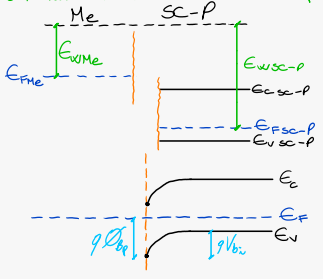
\includegraphics{Immagini_Micro&Nano/Imm_2_Fisica_dei_semiconduttori/giunzione radrizzante MeSCp.png}
    \caption{Giunzione raddrizzante Me-SCp: Diagramma a Bande}%
    \label{fig:Giunzione raddrizzante Me-SCp: Diagramma a Bande}
\end{figure}
%
\cleardoublepage%
%
\subsubsection{Contatti ohmici metallo-semiconduttore}
Per collegare la giunzione PN al mondo esterno è necessario fare delle metallizzazioni. il problema è che facendo qesto si crea un fenomeno fenomeno indesiderato dovuto ad un comportamento parassita.\\
Si supponga infatti, di realizzare un diodo pn e di volerlo connettere al resto del circuito tramite metallizzazione dei contatti.
La metallizzazione dei contatti crea due giunzioni metallo-SC, una con semiconduttore n e l'alto p. ma io sò che se Il lato SCn-metallo realizza una giunzione ohmica allora il contatto p-metallo realizza una giunzione rettificante (e viceversa).\\
La giunzione rettificante è un problema!
\begin{figure}[hbt!]
    \centering
     \begin{circuitikz} [scale=0.75]
        \draw(0,0) 
        to [short]++ (0.5,0) 
        to [short]++ (0,-0.5) rectangle++ (0.35,1)
        to [short]++ (0,-1.5) rectangle++ (2.5,2)
        rectangle++ (2.5,-2)
        to [short]++ (0,0.5) rectangle++ (0.35,1)
        to [short]++ (0,-0.5) to [short]++ (0.5,0);

        %label
        \node at(2.1,0) []{p};
        \node at(4.6,0) []{n};

        % ridisegno le connessioni per poterli colorare
        \draw[fill=gray] (0.5,-0.5) rectangle++ (0.35,1);
        \draw[fill=gray] (5.85,-0.5) rectangle++ (0.35,1);

        
        %disegno circuito equivalente
        \draw(0,-2.25) 
        to [D,bipoles/length=7mm]++ (2,0)
        to [D,bipoles/length=16mm]++ (2.5,0)
        to [R]++ (2,0);
        
    \end{circuitikz}
    \caption{Metallizzazione Me-SC: componenti parassiti}
    \label{fig: Metallizzazione Me-SC: componenti parassiti}
\end{figure}
E' necesario trovare una soluzione per trasformare il contatto rettificante in uno di tipo ohmico.
La soluzione più semplice sarebbe usare un metallo diverso durante la metallizzazione della giunzione drogata p, tuttavia non è una soluzione applicabile perchè La fabbricatura del Wafer non consente di distinguere diversi metalli senza aumentare notevolmente il costo di produzione.\\
Esiste invece una soluzione molto valida che consiste nell'aggiungere una regione fortememnte drogata prima della metallizzazione. Analizzando il caso n, per esempio.
All'aumentare del drogaggio del lato n, lo spessore della regione di carica spaziale diminuisce (è inversamente proporzionale a $\sqrt{N_D}$. Per un drogaggio sufficientemente elevato si ottiene una barriera tanto sottile da consentire il passaggio degli elettroni nelle due direzioni per effetto tunnel.\\

Quindi io applico tra SCn e Metallo una giunzione SCn+. lo strato n+ è così drogato da avere la banda di condizione sotto al livello di fermi, per cui si ottiene il diagramma a bande:

\begin{figure}[hbt!]
    \centering
    \begin{circuitikz}
        \draw(0.85,0.5) 
        to [short]++ (0,-1.5) rectangle++ (2.5,2)
        rectangle++ (1,-2)
        to [short]++ (0,0.5) rectangle++ (0.35,1)
        to [short]++ (0,-0.5) to [short]++ (0.5,0);

        %label
        \node at(2.1,0) []{n};
        \node at(3.9,0) []{$n^+$};

        % ridisegno le connessioni per poterli colorare
        \draw[fill=gray] (4.35,-0.5) rectangle++ (0.35,1);
        
        %disegno asse x
        %disegno asse y
        %disegno tratteggi
        \draw[densely dashed] (0.5,-3)--++ (4.75,0);
        \draw[densely dashed] (3.35,-1)--++ (0,-3.25);
        \draw[densely dashed] (4.35,-1)--++ (0,-3.25);
        \draw[densely dashed] (4.7,-0.5)--++ (0,-3.75);
        %disegno grafico
        \draw[very thick, red] (1,-2.5) node[left]{$E_C$}-- (2.9,-2.5)..controls (3.55,-2.5) and (3.3,-4).. (3.8,-4)
                             ..controls (4.3,-4) and (4.2,-1.5).. (4.35,-1.5);
        %label
        \draw[latex-latex,blue,thick] (4.35,-1.5) node[anchor=north west]{$\phi_{bn}$}-- (4.35,-3);
        %frecce
        \draw[-stealth,decorate,decoration={snake,amplitude=3pt,pre length=2pt,post length=3pt}] (5,-2.2) -- ++ (-2,0);
        \draw[stealth-,decorate,decoration={snake,amplitude=3pt,pre length=2pt,post length=3pt}] (5,-2.4) -- ++ (-2,0);

    \end{circuitikz}
    \caption{Metallizzazione Me-SC: drogaggio intermedio n+}
    \label{fig:Metallizzazione Me-SC: drogaggio intermedio n+}
\end{figure}


\begin{figure}[hbt!]
    \centering
     \begin{circuitikz}[scale=0.75]
        \draw(0,0) 
        to [short]++ (0.5,0) 
        to [short]++ (0,-0.5) rectangle++ (0.35,1)
        to [short]++ (0,-1.5) rectangle++ (2.5,2)
        rectangle++ (2.5,-2)
        rectangle++ (1,2)
        to [short]++ (0,-0.5) rectangle++ (0.35,-1)
        to [short]++ (0,+0.5) to [short]++ (0.5,0);

        %label
        \node at(2.1,0) []{p};
        \node at(4.6,0) []{n};
        \node at(6.4,0) []{$n^+$};

        % ridisegno le connessioni per poterli colorare
        \draw[fill=gray] (0.5,-0.5) rectangle++ (0.35,1);
        \draw[fill=gray] (6.85,-0.5) rectangle++ (0.35,1);

    \end{circuitikz}
    \caption{Metallizzazione Me-SC corretto}
    \label{fig: Metallizzazione Me-SC corretto}
\end{figure}
In questo modo la banda di conduzione vicino al metallo assume la forma a barriera di potenziale di spessore motlo sottile, favorendo il passaggio per effetto tunnel.\\
Gli elettroni possono attraversare questa giunzione per qualsiasi Va applicata come se fosse una giunzione ohmica.
\begin{figure}[hbt!]
    \centering
     \begin{circuitikz} [scale=0.75]
        \draw(0,0) 
        to [short]++ (0.5,0) 
        to [short]++ (0,-0.5) rectangle++ (0.35,1)
        to [short]++ (0,-1.5) rectangle++ (2.5,2)
        rectangle++ (2.5,-2)
        to [short]++ (0,0.5) rectangle++ (0.35,1)
        to [short]++ (0,-0.5) to [short]++ (0.5,0);

        %label
        \node at(2.1,0) []{p};
        \node at(4.6,0) []{n};

        % ridisegno le connessioni per poterli colorare
        \draw[fill=gray] (0.5,-0.5) rectangle++ (0.35,1);
        \draw[fill=gray] (5.85,-0.5) rectangle++ (0.35,1);
        
        %disegno circuito equivalente
        \draw(0,-2.25) 
        to [R]++ (2,0)
        to [D,bipoles/length=16mm]++ (2.5,0)
        to [R]++ (2,0);
        
    \end{circuitikz}
    \caption{Metallizzazione Me-SC corretto: parassiti ohmici}
    \label{fig: Metallizzazione Me-SC corretto: parassiti ohmici}
\end{figure}
%
\cleardoublepage%
%
\subsection{Capacità di giunzione per un diodo Schottky}
Il diodo schottky ha una capacità di diffusione nulla ($C_D=0$) ed una capacità di giunzione $C_j$ pari a quella di un semiconduttore PN con p molto drogato.\\
%
\noindent\begin{minipage}{0.5\textwidth}% adapt widths of minipages to your needs
La carica dovuta alla zona di svuotamento sarà
\begin{align}
    Q_j&=q\ N_D\ x_n=A \sqrt{q\ \mathcal{E}\ N_D\ 2(V_{bi}-V_A) }\\
    \intertext{Per cui la capacità di giunzione sarà:}
    C_j&=\left| \dfrac{dQ_j}{dV_A}\right|= A \sqrt{ \dfrac{q\ \mathcal{E}\ N_D}{2(V_{bi}-V_A)}}
\end{align}
\end{minipage}%
\hfill%
\begin{minipage}{0.3\textwidth}
    \begin{tikzpicture}[scale=0.5,transform shape]
             %disegno asse x
            \draw[->] (-2,0) node[anchor=north]{}-- (5,0)
            node[anchor=west]{$x$};
            %disegno asse y
            \draw[->] (0,-3.5)-- (0,3) node[anchor=south west]{$\rho_{fissa}(x)$};
            %disegno grafici
            \draw[thick,pattern=north east lines, pattern color=gray] (0,0)rectangle++ (4,2);
            \draw[-latex, line width=0.75mm,blue] (0,0)--++ (0,-3);
            %label
            \node at (4,0) [anchor=north]{$x_n$};
            \node at (0,2) [anchor=east]{$qN_D$};
            \node at (0,-2.5) [anchor=west]{$-qN_A$};
            \node at (2,1) [red]{$Q^+$};

            %disegno grafico energia
            %disegno asse x
            \draw[->] (-2,-5.5) node[anchor=north]{}-- (5,-5.5)
            node[anchor=west]{$x$};
            %disegno asse y
            \draw[->] (0,-9.5)-- (0,-3.7) node[anchor= west]{$\mathcal{E}(x)$};
            %disegno grafico rosso
            \draw[thick,red] (0,-9)-- (4,-5.5)-- (5,-5.5);
            %label
            \node at (0,-9) [anchor=west]{$\mathcal{E}_{MAX}=\dfrac{q\ N_D}{\varepsilon}x_n$};
            %disegno freccia del campo elettrico
            \draw[latex-] (0,-5)-- (4,-5) node[anchor= west]{$\mathcal{E}(x)$};
            
            %disegno grafico potenziale
            %disegno asse x
            \draw[->] (-2,-12.5) node[anchor=north]{}-- (6,-12.5)
            node[anchor=west]{$x$};
            %disegno asse y
            \draw[->] (0,-13.5)-- (0,-9.7) node[anchor= west]{$\phi(x)$};
            %disegno grafico tensione
            \draw[thick] (0,-12.5).. controls (1.5,-12.5) and (1,-10.7) .. (4,-10.5)--++ (1,0) node[anchor=west]{$q(V_{bi}-V_A)$};;
            
    \end{tikzpicture}
\end{minipage}
\begin{riepilogo}
    
\end{riepilogo}
\cleardoublepage%
\section{23.10.2023}
\section{BJT}
\subsection{Comportamento statico di un BJT}
Il transistore bipolare npn è costituito da due giunzioni n separate da un mezzo drogato p, viceversa quello pnp.\\

%
\noindent\begin{minipage}{0.7\textwidth}
    Il transistore, in generale, non è simmetrico per geometria e drogaggi e pertanto emettitore e collettore non sono interscambiabili.\\
\end{minipage}
\hfill
\begin{minipage}{0.29\textwidth}\raggedleft
    \begin{tikzpicture}
        \draw (0,0) rectangle++(1,1)node[pos=.5,, align=center]{$\scriptstyle N^+$ \\ E}
        rectangle++(0.75,-1)node[pos=.5, align=center]{$\scriptstyle P$ \\ B}rectangle++(1.25,1)node[pos=.5, align=center]{$\scriptstyle N$ \\ C};
    \end{tikzpicture}
\end{minipage}
%
Il BJT npn, essendo composto da due giunzioni pn (e quindi due diodi), può operare in 4 regioni di funzionamento:
\begin{enumerate}
    \item Interdizione
    \item Saturazione
    \item Regione attiva diretta (RAD)
    \item Regione attiva inversa (RAI)
\end{enumerate}
Per capire queste regioni di funzionamento, a seguito vengono mostrate gli schemi base del BJT.\\
\vspace{5mm}
\noindent\begin{minipage}{0.35\textwidth}
    \begin{circuitikz}[american,baseline=(current bounding box.center) ]
    \draw[](-0.5,0.75)node[left]{E} to[short]++(0.5,0);
        \draw (0,0) rectangle++(1.45,1.5)node[pos=.5,, align=center]{$n^+$}
        rectangle++(1,-1.5)node[pos=.5, align=center]{$p$}rectangle++(2.2,1.5)node[pos=.5, align=center]{$n$ };
        \draw(4.65,0.75) to[short]++(0.5,0)node[right]{C};
        %regione EB
        \draw[densely dotted](1.25-0.05,1.5)--++(0,-3.5);
        \draw[densely dotted](1.95-0.1,1.5)--++(0,-3.5);
        %regione BC
        \draw[densely dotted](2.65-0.25,1.5)--++(0,-3.5);
        \draw[densely dotted](3.65-0.25,1.5)--++(0,-3.5);
        %%%%%
        %disegno modello a diodi
        \draw(1.95,-3+.5)node[below]{B} to [short,-*]++(0,1) coordinate(b);
        \draw(b) to [D]++(-1+0.1,0)-|(-0.5,-2+.5)node[left]{E};
        \begin{scope}
        \ctikzset{bipoles/diode/height=0.7, bipoles/diode/width=0.7}
        \draw(b) to [D]++(2,0)-|(4.65+0.3,-2+.5)node[right]{C};
        \end{scope}
        
        %%%%%
        %disegno schema BJT
        \draw(0.9,-3.5) node[left]{E}
        --++(0.5,0) node[npn,anchor=E, rotate=-90, xscale=-1](npn1){}
        (npn1.B)--++(0,-0.5)node[right]{B}
        (npn1.C)--++(0.5,0) node[right]{C};
    \end{circuitikz}
\end{minipage}
\hfill%
\begin{minipage}{0.35\textwidth}\raggedleft
    \begin{circuitikz}[american,baseline=(current bounding box.center) ]
    \draw[](-0.5,0.75)node[left]{E} to[short]++(0.5,0);
        \draw (0,0) rectangle++(1.45,1.5)node[pos=.5,, align=center]{$p^+$}
        rectangle++(1,-1.5)node[pos=.5, align=center]{$n$}rectangle++(2.2,1.5)node[pos=.5, align=center]{$p$ };
        \draw(4.65,0.75) to[short]++(0.5,0)node[right]{C};
        %regione EB
        \draw[densely dotted](1.25-0.05,1.5)--++(0,-3.5);
        \draw[densely dotted](1.95-0.1,1.5)--++(0,-3.5);
        %regione BC
        \draw[densely dotted](2.65-0.25,1.5)--++(0,-3.5);
        \draw[densely dotted](3.65-0.25,1.5)--++(0,-3.5);
        %%%%%
        %disegno modello a diodi
        \draw(1.95,-3+.5)node[below]{B} to [short,-*]++(0,1) coordinate(b);
        \draw(b) to [D,invert]++(-1+0.1,0)-|(-0.5,-2+.5)node[left]{E};
        \begin{scope}
        \ctikzset{bipoles/diode/height=0.7, bipoles/diode/width=0.7}
        \draw(b) to [D,invert]++(2-0.1,0)-|(4.65+0.5,-2+.5)node[right]{C};
        \end{scope}
        %%%%%
        %disegno schema BJT
        \draw(0.9,-3.5) node[left]{E}
        --++(0.5,0) node[pnp,anchor=E,yscale=-1,xscale=-1,rotate=-90](pnp1){}
        (pnp1.C)--++(0.5,0) node[right]{C}
        (pnp1.B)--++(0,-0.5) node[right]{B};
    \end{circuitikz}
\end{minipage}


Interdizione e saturazione sono condizioni limite nelle quali il transistor è un interruttore aperto o chiuso

\subsubsection{Interdizione}
Si ottiene quando le giunzioni base-emettitore e base-collettore sono polarizzate inversamente.\\
In un BJT npn si raggiunge tale condizione se $V_{BE}<0, V_{BC}<0$\\
\textbf{il verso della tensione va dalla zona p alla zona n}.\\
In tali condizioni il transistore è in zona di interdizione.\\
La corrente di emettitore $I_E$ e di collettore $I_C$ sono le correnti inverse di saturazione dei due diodi, e $I_B = - I_E- I_C$. Pertanto tutte le correnti sono trascurabili ( CE è un circuito).

\subsubsection{Saturazione}
Si ottiene quando le giunzioni base-emettitore e base-collettore sono polarizzate direttamente.\\
In un BJT npn si raggiunge tale condizione se $V_{BE}>V_{th}, V_{BC}>V_{th}$ dove $V_{th}$ è la tensione di soglia dei due diodi\\
\textbf{il verso della tensione va dalla zona p alla zona n}.\\
In tali condizioni il transistore è in zona di saturazione.\\
In saturazione, le tensioni delle due giunzioni sono bloccate nell'intorno del valore di $V_{th}$ e la corrente che le attraversa è controllata dal circuito esterno.\\
La tensione di collettore è circa uguale alla tensione di collettore, pertanto si ha che $V_{CE}=V_{C}-V_{E} \approx 0$, questo significa che un circuito collegato ai capi di CE (che preleva $V_CE$) vedrà un circuito aperto.\\

Le altre due condizioni di funzionamento, sono proprie del BJT come dispositivo attivo, si devono analizzare tenendo presente l'interazione fra le due giunzioni

\subsubsection{Regione attiva diretta(RAD)}
Si ottiene quando la giunzione base-emettitore è polarizzata direttamente mentre la giunzione base-collettore è polarizzata direttamente.\\
Questo significa che nella giunzione base emettitore si ha iniezione di elettroni dall'emettitore alla base e iniezione di lacune dalla base all'emettitore.\\
Ora dobbiamo studiare due casi che si possono verificare al variare dello spessore della base $W_B$:\\

Se $W_B$ è molto maggiore della lunghezza di diffusione degli elettroni nella base si dice che le giunzioni BE e BC sono disaccoppiate tra loro.\\
In questa situazione gli elettroni in eccesso iniettati dall'emettitore nella base si ricombinano completamente nella base stessa, ossia non raggiungono la giunzione base-collettore.\\
Tutta la corrente di emettitore fluisce nella base la giunzione base-collettore, polarizzata inversamente, è attraversata dalla sola corrente di saturazione.\\

Se $W_B$ è molto minore della lunghezza di diffusione dei portatori minoritari iniettati nella base, $L_{n,B}$ per un npn.\\
In questo caso la maggior parte dei portatori iniettati non si ricombina, ma diffonde fino alla giunzione base-collettore, dove è catturata dal campo elettrico della regione di svuotamento associata alla giunzione base collettore e raccolta dal collettore.\\
l'interazione tra gionzione BE e BC si chiama effetto transistor.\\
In tale regione l'emettitore emette portatori attraverso la base del collettore, che i raccoglie; una piccola parte di tali portatori si ricombina nella base, dando luoco ad una corrente di lacune nella base.Si ha quindi:

\begin{align}
    |I_C| &\approx |I_E|
\end{align}
Ossia
\begin{align}
    |I_C| &=\alpha|I_E|
\end{align}
con $\alpha \leq 1$. pertanto:
\begin{align}
    |I_B|= |I_E|-|I_C|&=\dfrac{1-\alpha}{\alpha}|I_C|
\end{align}
%
ponendo $\beta=\dfrac{1-\alpha}{\alpha}$, si ha:
\begin{align}
    |I_C| &=\beta|I_B|
\end{align}
dove $\beta \gg 1$.\\
Piccole variazioni di corrente in base causano forti variazioni della corrente di collettore e di emettitore: il BJT in regione attiva diretta è un amplificatore di corrente pilotato in corrente

\subsubsection{Regione attiva inversa(RAI)}
non è di mio interesse, è inutile e meno efficiente del RAD. Se necessario leggere Ghione pagina 536.
\cleardoublepage

\subsection{Parametri caratteristici in RAD}
Indico con $F_n$ il flusso di elettroni attraverso una superficie (numero di elettroni per unità di tempo che attraversa la superficie), con $F_h$ il flusso di lacune.
Le relative correnti saranno $I_n=-qF_n$ e $I_h=qF_h$.\\
\begin{figure}[h]\centering
    \begin{tikzpicture}[scale=0.75]
        \draw(0,4) rectangle++(4.5,-4) rectangle++(3,+4) rectangle++(4.5,-4); %rettangolo di dimensione 12,4

        % disegno zona svuotamento EB
        \draw[pattern=north east lines, pattern color=gray](4.25,0) rectangle (4.75,4);
        % disegno zona svuotamento BC
        \draw[pattern=north east lines, pattern color=black](6,0) rectangle (9,4);
        
        %disegno corrente elett da E a B
        \coordinate[] (anEB) at (3.5,3);
        \coordinate[] (bnEb) at (5.15,3);
        \node[single arrow, draw=blue, very thick, fill=white,
        minimum width = 10pt, single arrow head extend=3pt,
        inner xsep=0pt,
        fit=(anEB) (bnEb)] {}; % length of arrow
        %label
        \node at (2.8,3) [blue]{$F_{nEB}$};

        %disegno corrente elett da B a C
        \coordinate[] (anBC) at (5.7,3);
        \coordinate[] (bnBC) at (9.35,3);
        \node[single arrow, draw=blue, very thick, fill=white,
        minimum width = 10pt, single arrow head extend=3pt,
        inner xsep=0pt,
        fit=(anBC) (bnBC)] {}; % length of arrow
        %label
        \node at (10.25,3) [blue]{$F_{nBC}$};

        %disegno corrente lacune da B a E
        \coordinate[] (ahBE) at (3.5,1);
        \coordinate[] (bhBE) at (5.25,1);
        \node[single arrow,draw=red, very thick, fill=white,
        minimum width = 10pt, single arrow head extend=3pt,
        inner xsep=0pt,rotate=180,
        fit=(ahBE) (bhBE)] {}; % length of arrow
        %label
        \node at (2.65,1) [red]{$F_{hBE}$};

        %altre correnti da B a C
        \draw[{Triangle[width=8pt,length=6pt]}-, line width=3pt](5.5,1.5) --++ (4.25, 0);
        %label
        \node at (10.45,1.5) [black]{$F_{hBC0}$};
        \draw[-{Triangle[width=8pt,length=6pt]}, line width=3pt](5.5,0.5) --++ (4.25, 0);
        %label
        \node at (10.45,0.5) [black]{$F_{nBC0}$};

        %ingressi e correnti di ingresso
        \draw [fill=gray!40!black] (-0.15,0.5) rectangle++ (0.15,3);
            \draw[thick] (-1,2) node[left]{E}
                 to [short,*-]++(1,0);
            \draw[>=latex,->] (-1,1.8)--++(0.75,0) node[anchor=north east]{$I_E$};
            
        \draw [fill=gray!40!black] (12,0.5) rectangle++ (0.15,3);
            \draw[thick] (13,2) node[right]{C}
                 to [short,*-]++(-1,0);
            \draw[>=latex,->] (13,1.8)--++(-0.75,0) node[anchor=north west]{$I_C$} ;
                 
        \draw [fill=gray!40!black] (5,-0.15) rectangle++ (2,0.15);
            \draw[thick] (6,-1.15) node[right]{B}
                 to [short,*-]++(0,1);
            \draw[>=latex,->] (5.8,-1.15)--++(0,0.75) node[anchor= north east]{$I_B$};

        %label NPN
        \draw[densely dotted](4.5,4)--++(0,1);
        \draw[densely dotted](7.5,4)--++(0,1);
        \node at (2.25,4.5)[]{N};
        \node at (6,4.5)[]{P};
        \node at (9.75,4.5)[]{N};
        
    \end{tikzpicture}
\caption{Flusso di elettroni e lacune in un BJT npn in RAD. Le regioni svuotate non sono proporzionalmente corrette ma è per dare l'idea}
\label{fig:Flusso di elettroni e lacune in un BJT npn in RAD}
\end{figure}

All'interno del BJT npn in RAD si distinguono diverse componenti di flusso delle particelle:
\begin{itemize}
    \item $F_{nEB}$ è il flusso di elettroni iniettati dall'emettitore alla base a causa della polarizzazione diretta della giunzione B-E;
    
    \item $F_{hBE}$ è il flusso di lacune iniettate dalla base all'emettitore a causa della polarizzazione diretta della giunzione base emettitore. \textbf{è una componente indesiderata}/parassita perchèncontribuisce all'aumento di $I_B$ ma non all'aumento di $I_C$. In altre parole: il contributo di  $I_E$ che si crea grazie ad $F_{hBE}$ non raggiunge il collettore, ma è raccolta nell'emettitore. pertanto una variazione di questo flusso causata dalla corrente $I_B$ non influisce sulla corrente di collettore.
    
    \item $F_{nBC}$ è il flusso di elettroni che, attraversata la base, raggiungono la giunzione base-collettore. Se la base è sottile rispetto alla lunghezza di diffusione degli elettroni, la maggior parte degli elettroni non si ricombina nella base con le lacune ma viene raccolta dal collettore.\\
    lE LACUNE CHE SI RICOMBINANO CON GLI ELETTRONI INIETTATI NELLA BASE danno luogo alla sola componente utile della corrente di base
    \begin{ricevimento}
        spiegare ultima frase
    \end{ricevimento}
    \item $F_{nBC0}$ e $F_{hCB0}$ sono gli elettroni e le lacune che attraversano la giunzione B-C quando l'emettitore è aperto. Sono quindi le componenti della piccolissima corrente inversa di saturazione della giunzione B-C.\\
    Sono componenti parassite perchè non pilotate dalla corrente di base ed hanno un valore trascurabile in regione attiva diretta ma divengono le componenti principali in regione attiva inversa (che non si studia).
    
\end{itemize}
Tenendo presente che le correnti sono considerate entranti (figura \ref{fig:Flusso di elettroni e lacune in un BJT npn in RAD}), si ha:
allora il flusso totale di cariche che entra nell'emettitore sarà:
mentre il flusso totale di cariche che entra nel collettore
\begin{align}
F_E &= F_{nEB}-F_{hBE}\\
    F_C &= -F_{nBC}-F_{nBC0}+F_{hCB0}
\end{align}
\begin{ricevimento}
    Fe ed Fc li devo moltiplicare per +q o -q?
\end{ricevimento}
per ottenere le cariche moltiplico tutto per q, ricordando che le lacune hanno segno positivo mentre gli elettroni hanno segno negativo.:
\begin{align}
I_E &= (-q)F_{nEB}+q(-F_{hBE})\\
    I_C &= (-q)(-F_{nBC})+(-q)(-F_{nBC0})+qF_{hCB0}
\end{align}
Ovvero:
\begin{align}
I_E &= -qF_{nEB}-qF_{hBE}\\
    I_C &= qF_{nBC}+qF_{nBC0}+qF_{hCB0}
\end{align}
Dove chiamo $I_{CB0}=qF_{nBC0}+qF_{hCB0}$ la corrente inversa di saturazione della giunzione base collettore (è quella che si misura fra C-B quando E è aperto) ed è importante perchè il contributo di corrente di elettroni inversa si mescola con quello che arriva all'emettitore.\\ allora:
\begin{align}
    I_C &= qF_{nBC}+I_{CB0}
\end{align}
   
Dando un'occhiada al modello a diodi di un BJT npn, si nota come le correnti possano essere calcolate dalla legge di Khirchoff:
\begin{align}
    I_B &= -I_E-I_C
\end{align}
ossia:
\begin{align}
     I_B &= qF_{hBE}+\-I_{CB0}
\end{align}
Dove $qF_{nEB}-qF_{nBC}$ rappresenta il numero di elettroni che si ricombinano in base.
\begin{psbox}
\textbf{La corrente di base nasce per mantenere l'eccesso di continuo rifornimento di lacune che si ricombinano con gli elettroni di EB}
    Per questo si dice spesso che il BJT è pilotato in corrente  ma non è appropriato usare questa frase!\\
    il transistor è pilotato in tensione, ma le giunzioni hanno una forte variazione in corrente e questo implica che serve molta precisione per regolare la corrente , quindi spesso si pilota in corrente
    \begin{ricevimento}
        Spiegare meglio?
    \end{ricevimento}
\end{psbox}
Adesso definiamo dei parametri importanti:
\begin{itemize}
    \item Efficienza di emettitore  
    \begin{equation}
        \label{eqn:efficienza di emettitore}
        \gamma = \dfrac{F_{nEB}}{F_{nEB}+F_{hBE}}
    \end{equation}
    è il rapporto tra la corrente associata ai portatori (elettroni) iniettati dall'emettitore nella base e le correnti totali che attraversano la giunzione Base-Emettitore. Idealmente $\gamma=1$ ma, realisticamente parlando sarebbe $\gamma < 1$

    \item Fattore di trasporto in base 
    \begin{equation}
        \label{eqn:fattore di trasporto in base}
        b=\dfrac{F_{nBC}}{F_{nEB}}
    \end{equation}
    è il rapporto tra la corrente di elettroni che dalla base va all'emettitore e la corrente di elettroni che dall'emettitore va dentro la base.\\
    Idealmente dovrebbe essere 1.
    \item amplificazione di corrente a base comune $\alpha$
    \begin{equation}
        \label{eqn:amplificazione di corrente a base comune}
     \alpha = \dfrac{F_{nBC}}{F_{nEB}+F_{hBC}} = b \gamma
    \end{equation}
    è espresso come rapporto tra la corrente di collettore e quella di emettitore nel caso in cui non ci siano correnti di saturazione inversa.\\
    idealmente è 1 ma realisticamente è minore di 1.\\

    Siccome è chiamato amplificatore sembra difficile che sia un parametro minore di 1.Non si ha amplificazione assumento come ingresso $I_E$ e come uscita $I_C$. l'amplificazione i corrente è in realtà $\beta$ (che è descritto dopo) assumento $I_C$ come uscita ed $I_B$ come corrente di ingresso
    
    \item amplificazione di corrente a emettitore comune $\beta$
    \begin{equation}
        \label{eqn:amplificazione di corrente a emettitore comune}
        \beta = \dfrac{\alpha}{1-\alpha}
    \end{equation}
\end{itemize}
Tenendo presente dal'equazione \ref{eqn:fattore di trasporto in base} che:
 \begin{equation}
     F_{nBC}=b \ F_{nEB}
 \end{equation}
e dall'equazione \ref{eqn:efficienza di emettitore} che:
\begin{equation}
    F_{nEB}+F_{hBE}=\dfrac{F_{neB}}{\gamma}
\end{equation}
si ha:
\begin{align}
    I_E &= -qF_{hBE}-qF_{nEB}= - \dfrac{-qF_{nEB}}{\gamma}\\
    I_C &= qbF_{nEB}+I_{CB0}
\end{align}

da cui, eliminando $F_{nEB}$:

\begin{equation}
    I_C=-\gamma b I_E + I_{CB0}\label{eq:formula Ic ebers-moll}
\end{equation}

Adesso, ricordo che $\alpha = \gamma b $ e che $alpha \approx 1$ allora la corrente $I_C$ si può approssimare come
\begin{equation}
    I_C=-\gamma b I_E + I_{CB0} \approx - \alpha I_E
\end{equation}

considerando quindi la legge di Khirchoff, si può portare in funzione di $I_B$:
\begin{align}
    I_B&=-I_E-I_C \\
    I_C&= \dfrac{\alpha}{1-\alpha}I_B + \dfrac{1}{1-\alpha}I_{CB0} 
\end{align}
    Usando l'equazione (\ref{eqn:amplificazione di corrente a emettitore comune}):
\begin{align}
    I_C&= \beta I_B + (1+\beta)I_{CB0}
\end{align}

Quindi la corrente di collettore è composta da una corrente di saturazione inversa amplificata di $\beta +1$. Questo rappresenta un problema visto che $\beta$ è alto e $I_{CB0}$ dipende dalla temperatura e provoca il \textbf{ runaway termico} :
se T aumenta, $I_{CB0}$ aumenta quindi $I_C$ aumenta facendo aumentare la potenza dissipata e di conseguenza la temperatura. E' un cane che si morde la coda.\\

\begin{psbox}
    Per risolvere questo problema si può mettere una reisstenza di emettitore o base che realizza un feedback negativoche riduce la tensione Vbe.
    figure e pro e contro delle due configurazioni
\end{psbox}

\cleardoublepage
\subsubsection{BJT dal punto di vista delle bande}
Come funziona in linea generale:
In condizionid i equilibrio si instaura, tra le giunzioni base-emettitore e base-collettore, una potenziale di giunzione.

\begin{figure}[hbt!]
    \centering
    \begin{tikzpicture}
    \begin{scope}[scale=1.25]
        \draw[](-0.5,0.75)node[left]{E} to[short]++(0.5,0);
        \draw (0,0) rectangle++(1.45,1.5)node[pos=.5,, align=center]{$n^+$}
        rectangle++(0.75,-1.5)node[pos=.5, align=center]{$p$}
        rectangle++(2.2+0.3,1.5)node[pos=.5, align=center]{$n$ };
        \draw(4.7,0.75) to[short]++(0.5,0)node[right]{C};
        %regione EB
        \draw[densely dotted](1.3,1.5)--++(0,-10);
        \draw[densely dotted](1.65,1.5)--++(0,-10);
        %regione BC
        \draw[densely dotted](2.15,1.5)--++(0,-10);
        \draw[densely dotted](3.15,1.5)--++(0,-10);
        %diagramma a bande in equilibrio
        \draw (0,-2+0.5)--(1.1,-2+0.5) to [out=0, in=180](1.75,-1+0.5)--(2.15,-1+0.5)to [out=0, in=180](3.15,-2+0.5)--(4.7,-2+0.5);
        \draw (0,-3.1+0.5)--(1.1,-3.1+0.5) to [out=0, in=180](1.75,-2.1+0.5)--(2.15,-2.1+0.5)to [out=0, in=180](3.15,-3.1+0.5)--(4.7,-3.1+0.5);
        %diagramma a bande NON in equilibrio
        \draw (0,-4.5)--(1.1,-4.5) to [out=0, in=180](1.75,-4)--(2.15,-4)to [out=0, in=180,distance=0.6 cm](3.15,-6)--(4.7,-6);
        \draw (0,-5.6)--(1.1,-5.6) to [out=0, in=180](1.75,-5.1)--(2.15,-5.1)to [out=0, in=180,,distance=0.6 cm](3.15,-7.1)--(4.7,-7.1);
        %livelli di fermi
        
        %label diffusione elettroni
        \draw[-latex](1,-3.25)--++(0.75,0)node[align=center, anchor=south east]{Diffusione \\ elettroni};
        %label deriva elettroni
        \draw[-latex](2,-3.25)to[out=0, in=110]++(1.5,-2)node[align=center, anchor=south west]{deriva \\ elettroni};
    \end{scope}

    %diagramma a bande non in equilibrio
    \end{tikzpicture}
    \caption{Caption}
    \label{fig:enter-label}
\end{figure}
Se poi supponiamo di avere un BJT in RAD, avrò la giunzione BE attiva e la giunzione BC spenta risultando nel grafico in figura (b).\\
Gli elettroni dell'emettitore si diffondono per diffusione verso la base mentre si spostano dalla base verso il collettore per effetto deriva. 
una volta che gli elettroni hanno raggiunto la regione di svuotamento B-C vengono attratti dal compo elettrico nella direzione di C(scivolo potenziale). \\
modificando Vbe regolo la popolazione di elettroni in base (e quindi quelli che arriveranno al collettore se la base è corta)e quindi la raccolta. ma Vbc in prima approssimazione non si modifica. si hanno delle correnti costanti in funzione di vbc, le correnti Ie circa= I applicata.
Quindi per far si che vi sia corrente in uscita si deve rendere nulla la corrente la correnteproveniente dal C nella B (mandando in cut off la giunzione corrispondente) altrimenti le correnti si annullerebbero
\begin{figure}[hbt!]
    \centering
    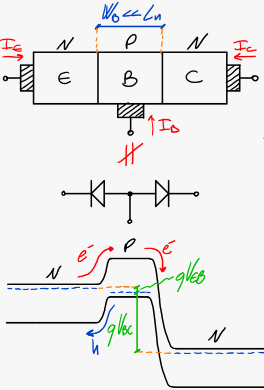
\includegraphics{Immagini_Micro&Nano/Imm_3_Transistor_BJT/BJTNPN.png}
    \caption{Diagramma a bande di un BJT npn}
    \label{fig:Diagramma a bande di un BJT npn}
\end{figure}
 \cleardoublepage
Gli elttroni dall'emettitore passano nella base grazie al potenziale $V_{EB}$ che riduce la barriera di potenziale su E-B.\\
Questi elettroni si ritroveranno nella base ed in parte si ricombineranno con le lacune ma, grazie al fatto che la base è corta, molti riescono ad arrivare alla regione di svuotamento B-C che è praticamente uno scivolo (grazie alla presenza di $V_{BC}$ che dirige/lancia gli elttroni e li fà entrare in C).\\
Questo processo è tanto più efficacie quanto più la base è sottile. Inoltre, si capisce che, regolando la $V_{BE}$ regolo anche il numero di elettroni iniettati e quindi regolo la corrente di emettitore.
se la base è corta allora tale corrente sarà la $I_C$ cioè la corrente di soglia. E' importante marcare che ho fatto una grossa approssimazione: all'aumentare di $V_{BC}$,  la $I_C$ rimane costante.
\begin{psbox}
Se agisco sulla qVbc gli elettroni una volta raggiunta la I\_c cadono comunque in C: 
\begin{ricevimento}
    spiegare
\end{ricevimento}
    \begin{center} 
       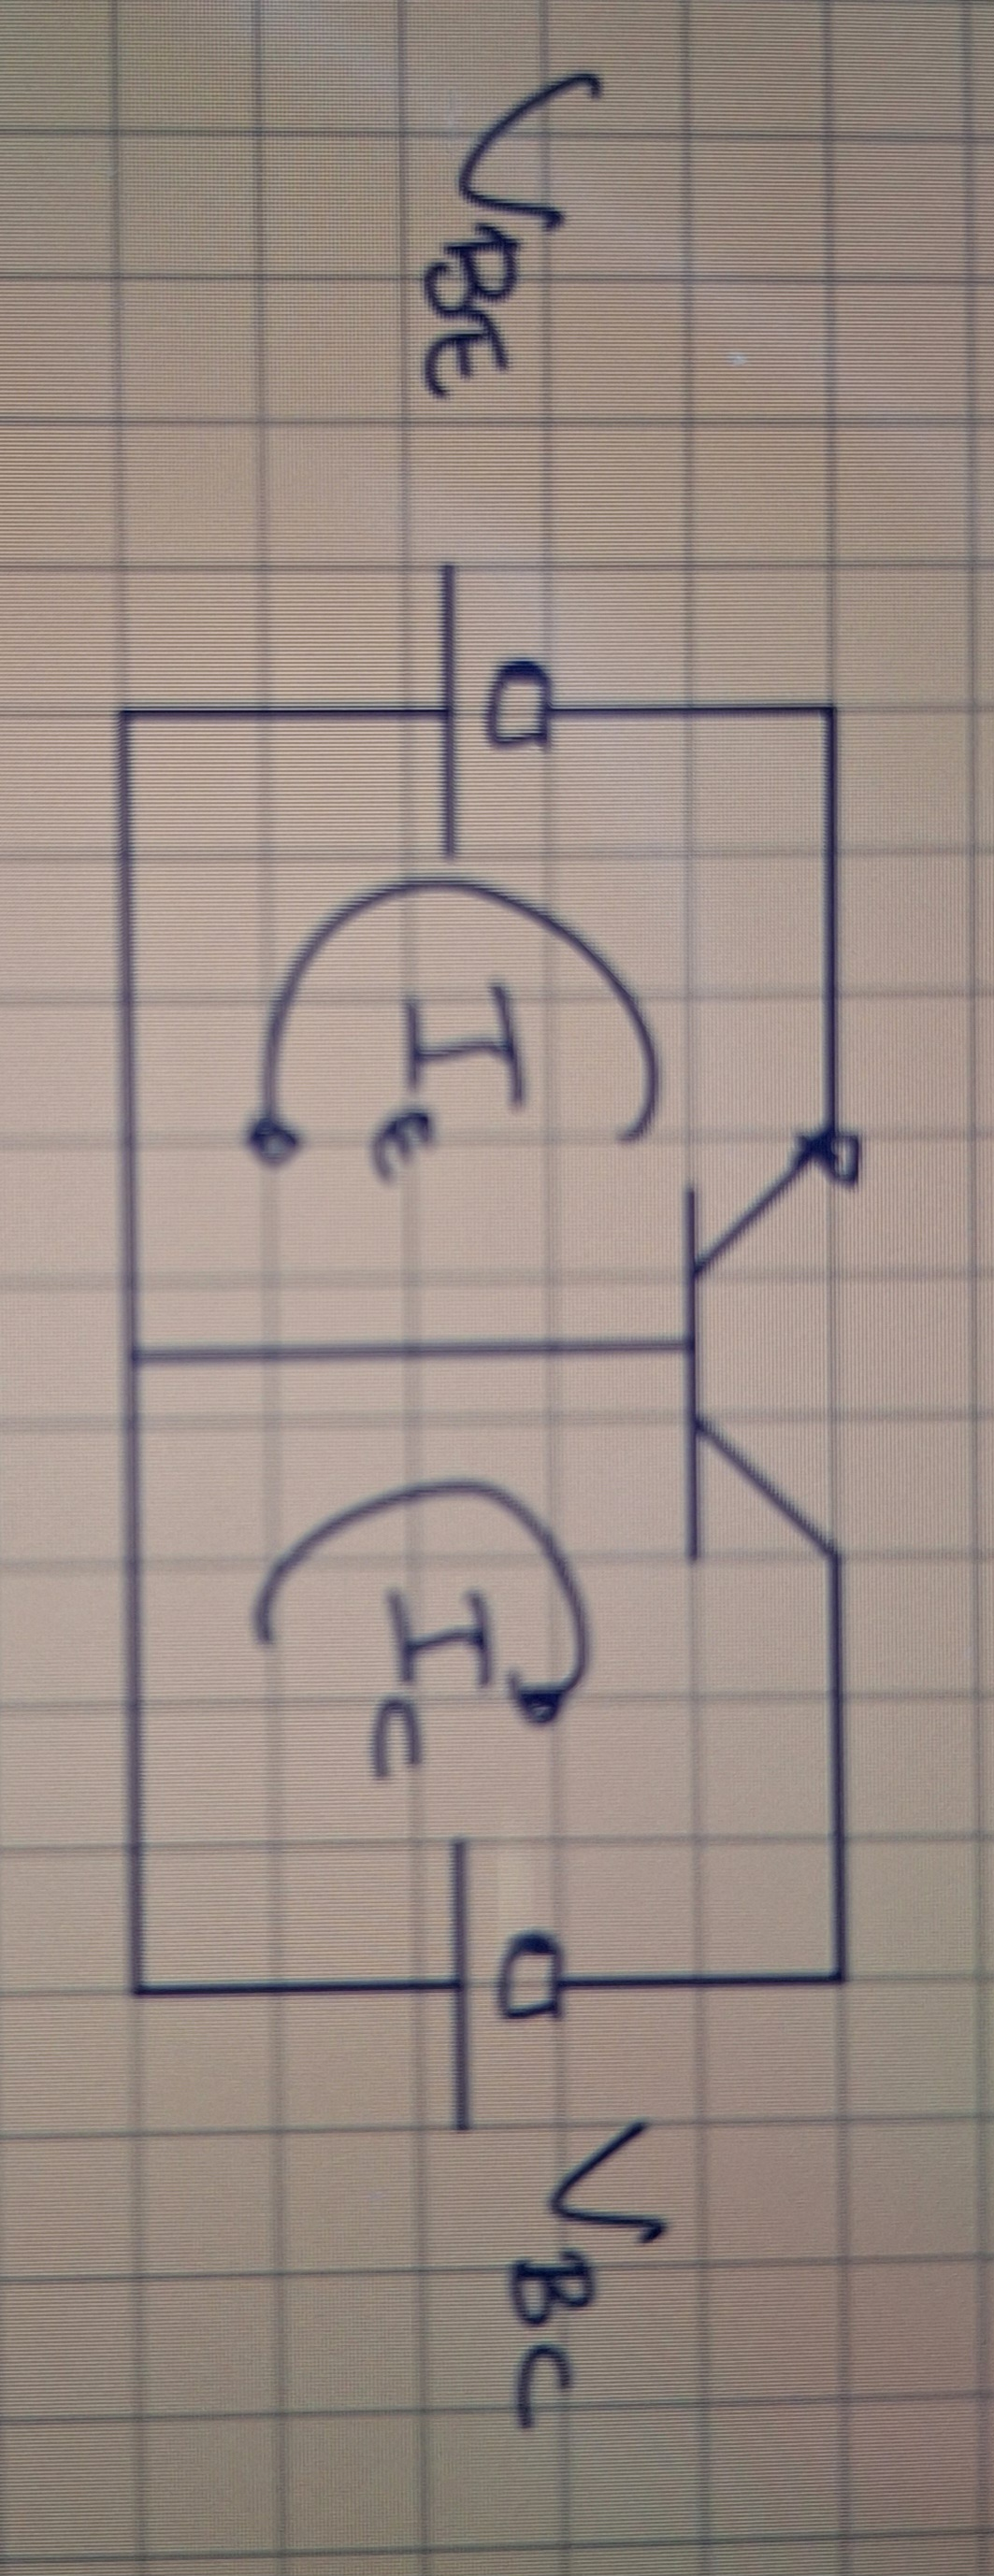
\includegraphics[width=0.25\textwidth,angle=90]{Immagini_Micro&Nano/Imm_3_Transistor_BJT/polarizzazBJTRAD.png}
       \vspace{5mm}
        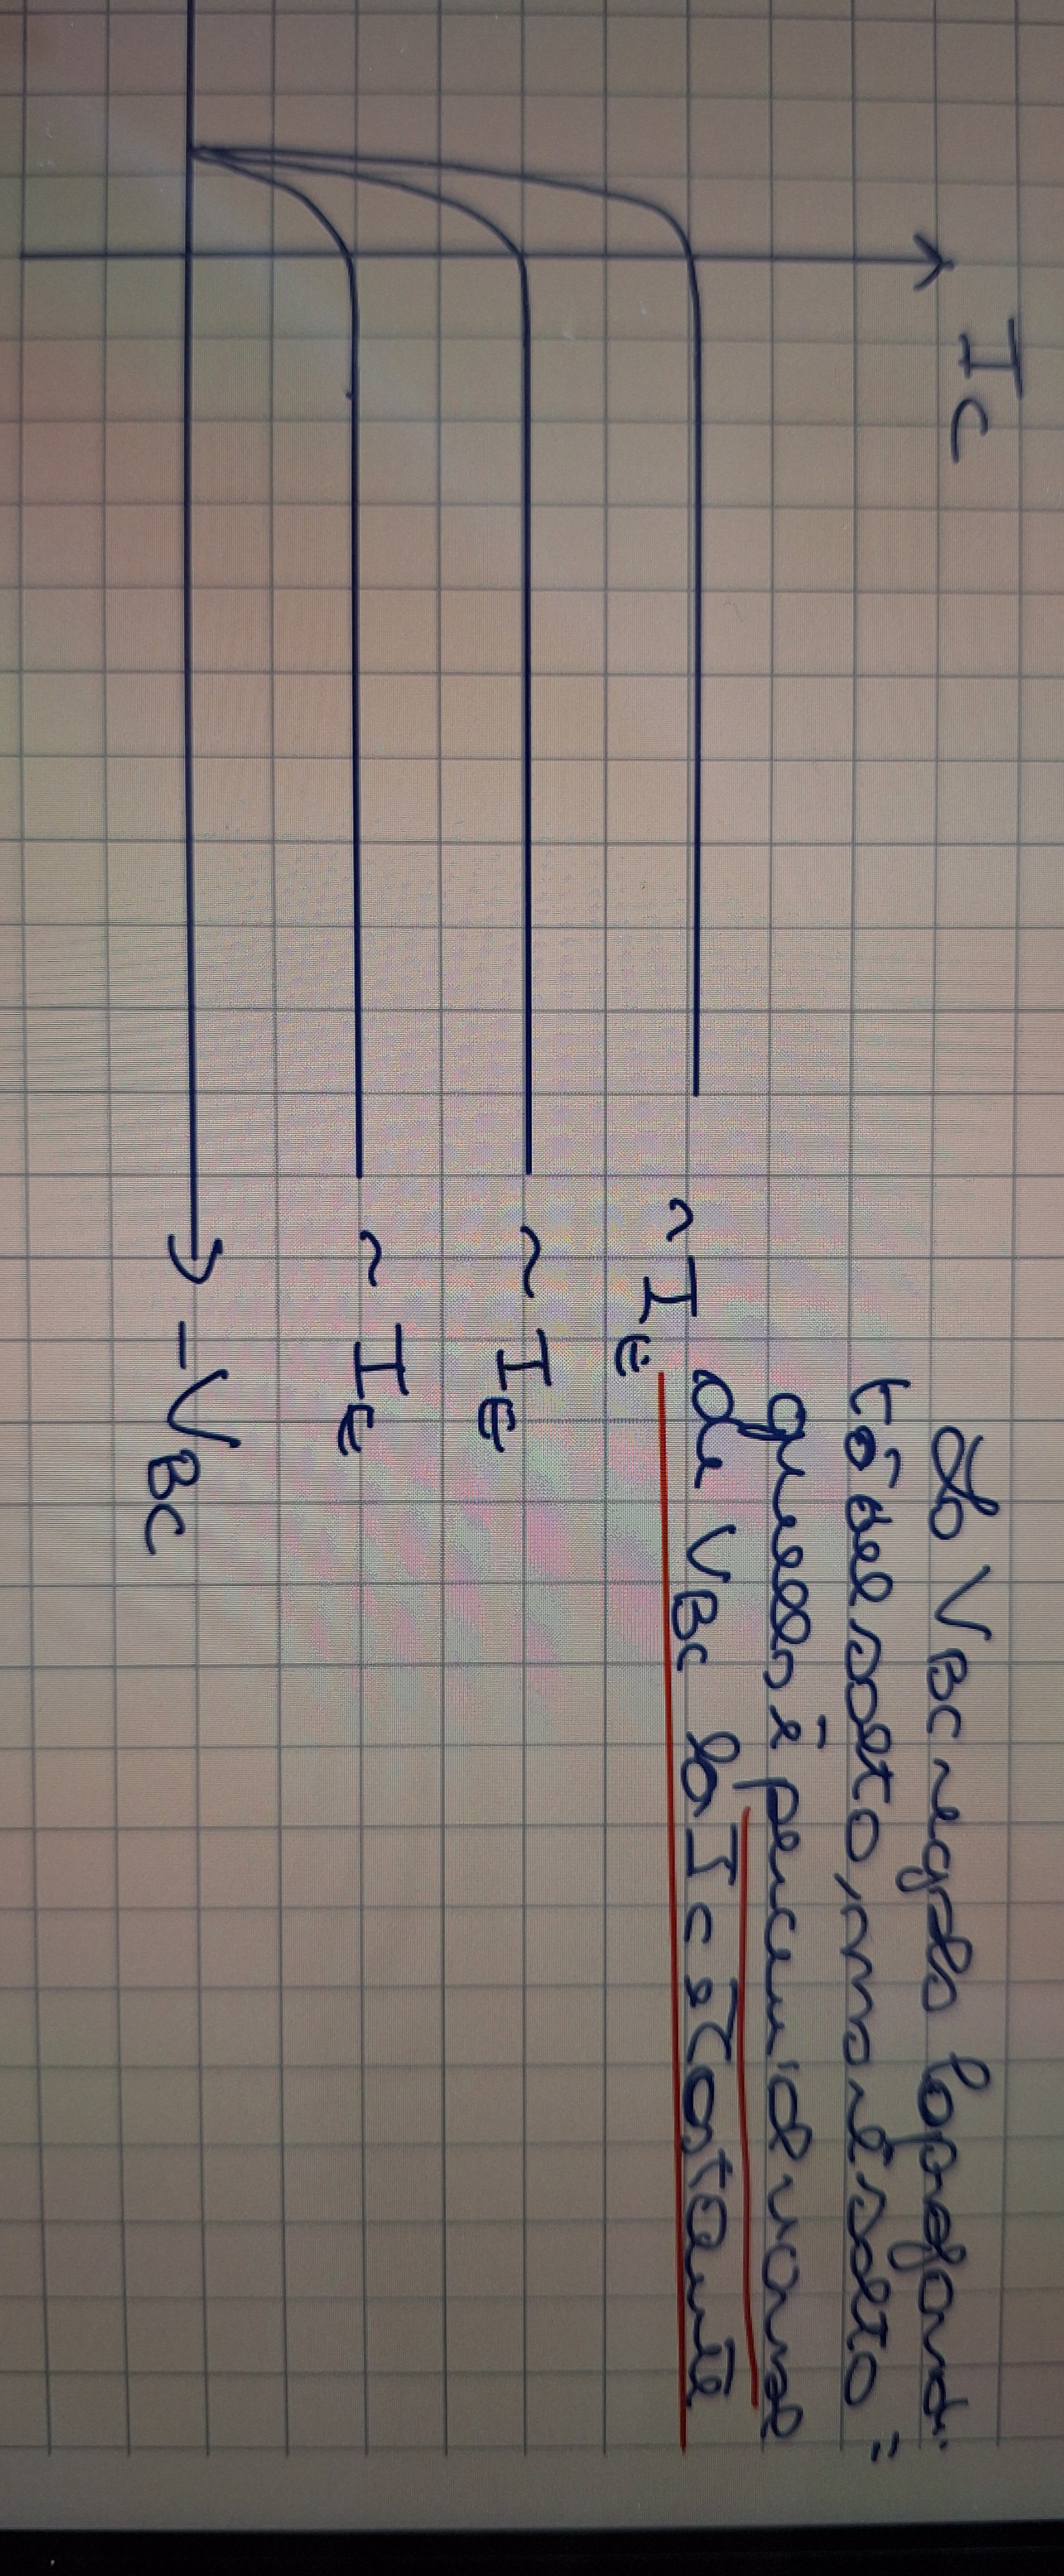
\includegraphics[width=0.25\textwidth,angle=90]{Immagini_Micro&Nano/Imm_3_Transistor_BJT/caratteristicaBJTRAD.png}
    \end{center} 
\end{psbox} 

Ignorando le zone di svuotamento avrò un profilo dei portatori minoritari come in figura:
\begin{figure}[hbt!]
    \centering
    \begin{tikzpicture}[scale=1]
        \draw(0,0)--++(12,0);
        \draw(4,0)--++(0,3.5)node[above]{$X_E$};
        \draw(8,0)--++(0,3.5)node[above]{$X_C$};
        
        \draw[dashed](0,0.5)--++(4,0);
        \draw[dashed](4,0.5)--++(4,0);
        \draw[dashed](8,0.5)--++(4,0);

        \node at (2,3.5)[]{N};
        \node at (6,3.5)[]{P};
        \node at (10,3.5)[]{N};

        %grafico rosso
        \draw[very thick,red] (4,2.5) to [out=240,in=1] (0,0.55) ;
        % label formula
        \node at (4,2.8)[left]{$pn_0e^{\dfrac{V_{be}}{V_T}}$};
        \draw[very thick,red] (4,2.5).. controls (5,1.5) and (5.7,1.55) .. (6,1.45);
        %cerchio
        \node[circle,fill=black,inner sep=0pt,minimum size=4pt] at (4,2.5)[]{};
        % label formula
        \node at (4,2.8)[right]{$np_0e^{\dfrac{V_{be}}{V_T}}$};
        \draw[very thick,red] (6,1.45) to [out=-5,in=120] (8,0) ;
         %cerchio
        \node[circle,fill=black,inner sep=0pt,minimum size=4pt] at (8,0)[]{};
        % label formula
        \node at (6.5,-0.32)[right]{$np_0e^{\dfrac{V_{be}}{V_T}}$};
        \draw[very thick,red] (8,0) to [out=17,in=180] (12,0.45) node[right,black]{$pn_0$};
       
        % label formula
        \node at (8,-0.32)[right]{$pn_0e^{\dfrac{V_{bc}}{V_T}}$};

        %carica
         \draw[pattern=north east lines, pattern color = gray] (4,0)--(4,2.5).. controls (5,1.5) and (5.7,1.55) .. (6,1.45)to [out=-5,in=120] (8,0)--(4,0); 
         \node at (5.5,1)[] {$\textbf Q_B$};
         

         %freccie e label
         \draw[>=latex, <->] (0,-0.25)--(3.9,-0.25); \node at (2,-0.25)[anchor=north]{$W_E$};
         \draw[>=latex, <->] (4.1,-0.25)--(7.9,-0.25); \node at (6,-0.25)[anchor=north]{$W_B$};
         \draw[>=latex, <->] (8.1,-0.25)--(12,-0.25); \node at (10,-0.25)[anchor=north]{$W_C$};

         \draw[>=latex, <-,blue] (4,-0.1)--++(0,-0.5) node [anchor=north,blue]{$on$};
         \draw[>=latex, <-,blue] (8,-0.1)--++(0,-0.5) node [anchor=north,blue]{$off$};
         
    \end{tikzpicture}
    \caption{Caption}
    \label{fig:enter-label}
\end{figure}

Ora ricordo che la corrente è data dalla la variazione di carica nel tempo.\\
Prima di continuare  definisco due parametri di tempo che serviranno per studiare la variazione di carica nella base:
\begin{itemize}
    \item $\tau_t$: tempo di transito in base. E' il tempo medio impiegato dai portatori minoritari (elettroni iniettati nella base dall'emettitore) per attraversare la zona neutrale della base e raggiungere il limite della regione di svuotamento della giunzione base-collettore. 
    \item $\tau_0$: tempo di vita medio dei portatori minoritari nella base ($\tau_n$ per un npn, $\tau_h$ per un pnp). 
\end{itemize}
%
Le cause che provocano la variazione nel tempo della carica mobile all'interno della base sono due.\\
La prima è dovuta al transito dei portatori dalla giunzione emettitore-base verso la giunzioene base-collettore:
\begin{equation}
    \left.\dfrac{dQ_B}{dt}\right|_t= -\dfrac{Q_B}{\tau_t}
\end{equation}
La seconda causa si riferisce al fenomeno della ricombinazione che ha effetto sulle cariche mobili iniettate nella base dall'emettitore:
\begin{equation}
    \left.\dfrac{dQ_B}{dt}\right|_R= -\dfrac{Q_B}{\tau_0}
\end{equation}
Perché il transistore funzioni correttamente è necessario che la variazione di carica per effetto della ricombinazione sia molto minore della variazione di. carica per effetto del transito. Infatti si ha, trascurando la $I_{CB0}$: 

\begin{align}
    |I_C|&= -\left.\dfrac{dQ_B}{dt}\right|_t= \dfrac{Q_B}{\tau_t}
    \end{align}
    mentre, trascurando la componente della corrente di base dovuta alle lacune if1iettate nell'emettitore (ossia ponendo $\gamma \approx 1$): 
\begin{align}
    |I_B|&= -\left.\dfrac{dQ_B}{dt}\right|_R= \dfrac{Q_B}{\tau_0}
\end{align}

\begin{psbox}
    ricordo, dall'equazione di continuità che \[ \dfrac{dQ}{dt}= \nabla \cdot J\]. Nel caso monodimensionale esso si traduce in \[\dfrac{dQ}{dt}=\dfrac{dJ}{dx}\]
\end{psbox}
nell'immediato 
\begin{equation}
    \beta=\dfrac{I_C}{I_B} \approx \dfrac{\tau_0}{\tau_T}
\end{equation}
quindi $\beta \uparrow$ se $\tau_0 \uparrow$ e $\beta \downarrow$ se $\tau_T \uparrow$. tuttavia per avere bjt veloce servirà $\tau_0 \downarrow$, ecco che capisco che bisogna fare un compromesso

\subsubsection{Come calcolare Le correnti del BJT  in modo analitico}
Seguirò gli stessi ragionamenti fatti nel caso di giunzione PN ma applicando, più avanti, un'opportuna semplificazione delle correnti di diffusione (in questo caso corrente di lacune).\\
Si parte considerando la corrente di diffusione delle lacune nell'emettitore:
\begin{equation}
    I_{P,D}=-qD_P\dfrac{dp}{dx}
\end{equation}
Dove $D_P$ è la diffusività delle lacune mentre $\frac{dp}{dx}$ indica la variazione spaziale della concentrazione di lacune.\\
E' possibile semplificare il calcolo seguendo due considerazioni:\\
\begin{enumerate}
    \item Innanzitutto, considero la lunghezza dell'emettitore come fosse corta laddove le cariche si diffondono. Questo vuoldire che \textbf{la lunghezza di diffusione delle lacune nell'emettitore è molto minore(maggiore?) della dimensione fisica dell'emettitore($W_E$)}.
la medesima cosa si applica agli elettroni nella base e alle lacune nel collettore. Quindi:
\begin{align}
    Lp_{E} & \ll W_E\\
    Ln_B &\ll W_B \\
    Ln_C &\ll W_C
\end{align}
\item Inoltre, devo ricordare che il terminale sinistro dell'emettitore dovrà essere metallizzato per permettere la connessione con mondo esterno, creando la giunzione Schottky.
La metallizzazione ci costringe a considerare le condizioni a contorno che si formano con il metallo, infatti i portatori minoritari in eccesso, che altrimenti contribuirebbero alla corrente di diffusione, vengono raccolti o bloccati dal metallo, influenzando così le condizioni di contorno e semplificando l'analisi.\\
%
\end{enumerate}


\begin{ricevimento}
    qui mi sono perso
\end{ricevimento}
Detto questo, posso approssimare la concentrazione dei portatori con andamento esponenziale, come se  avessero l'andamento di una retta, consentendomi di semplificare la derivata presente all'interno della $I_{P,D}$.



\begin{figure}[hbt!]
    \centering
    \begin{subfigure}[]{0.49\textwidth}
        \centering
        \begin{tikzpicture}[scale=1]
        
            \draw(0,0)--++(4,0);
            \draw(4,0)--++(0,3);
            
            \draw[dashed](0,0.5)--++(4,0);
    
            %grafico rosso
            \draw[very thick,red] (3.9,2.9) to [out=270,in=1] (0,0.55) ;
            % label formula
            \node at (3.8,2.8)[left]{$pn_0e^{\frac{V_{be}}{V_T}}e^{-x/L_n}$};

             %freccie e label
             \draw[>=latex, <->] (0,-0.25)--(3.9,-0.25); \node at (2,-0.25)[anchor=north]{$W_E \gg L_n$};
             \draw[>=latex, <-,blue] (4,-0.1)--++(0,-0.5) node [anchor=north,blue]{$x_{EB}$};

             %metallizzazione
             \draw[densely dashed](1,3)--++(0,-3);
             \draw [fill=gray](1,1) rectangle++(-0.10,1);
        \end{tikzpicture}
        \caption{reale}
        \label{fig:enter-label}
    \end{subfigure}
    %
    \begin{subfigure}[]{0.49\textwidth}
        \centering
        \begin{tikzpicture}[scale=1]
            \draw(0,0)--++(4,0);
            \draw(4,0)--++(0,3);
            
            \draw[dashed](0,0.5)--++(4,0);
    
            %grafico rosso
            \draw[very thick,red] (4,2.5) -- (1,0.55) ;
            % label formula
            \node at (4,2.8)[left]{$pn_0e^{\dfrac{V_{be}}{V_T}}$};
            
            %cerchio
            \node[circle,fill=black,inner sep=0pt,minimum size=4pt] at (4,2.5)[]{};
 
             %freccie e label
             \draw[>=latex, <->] (1,-0.25)--(3.9,-0.25); \node at (2.5,-0.25)[anchor=north]{$W_E \ll L_n$};
             \draw[>=latex, <-,blue] (4,-0.1)--++(0,-0.5) node [anchor=north,blue]{$x_{EB}$};

             %metallizzazione
             \draw[densely dashed](1,3)--++(0,-3);
             \draw [fill=gray](1,1) rectangle++(-0.10,1);
        \end{tikzpicture}
        \caption{approssimato}
        \label{fig:enter-label}
    \end{subfigure}
    
    \caption{Caption}
    \label{fig:enter-label}
\end{figure}
%
La variazione della concentrazione di portatori minoritari nella regione metallizzazione di emettitore fino all'inizio della regione svuotata ($x_{EB}$), può essere calcolata come il semplice rapporto "Base $\cdot$ altezza":
\begin{equation}
    \left. \dfrac{dp}{dx}\right|_{x_{EB}}=\dfrac{pn_0 \cdot e^{\dfrac{V_{BE}}{V_T}}}{W_E}
\end{equation}
Se il transistor è fatto bene ed è sufficientemente piccolo, tale approssimazione diventa praticamente il risultato corretto (vero).\\
La corrente approssimata risulterà essere:
\begin{equation}
    I_{P,D}=-qD_P \dfrac{pn_0 \, e^{\dfrac{V_{BE}}{V_T}}}{W_E}
\end{equation}
%
Secondo la teoria di Shockley della giunzione pn, le correnti di emettitore e collettore in un transistore bipolare sono approssimate come somma delle due correnti
di diffusione dei portatori minoritari ai bordi delle regioni di svuotamento delle
rispettive giunzioni (ossià in $x_{EB}$ e in $x_{BE}$ per la giunzione di emettitore, in $x_{BC}$
e $x_{CB}$ per la giunzione di collettore.\\
Si ha allora, tenendo presente che le densità di corrente sono definite positive verso destra,
concorde con $I_E$ ma discorde con $I_C$: 
%
\begin{equation}
    I_E= I_{h,D}(x_{EB}) + I_{n,D}(x_{BE})
\end{equation}
%
\begin{equation}
    -I_C= I_{n,D}(x_{BC}) + I_{h,D}(x_{CB})
\end{equation}
%
Ora devo trovare un modo per risolvere queste correnti.\\
Dalla definizione di corrente di diffusione:
\begin{align}
    I_{h,D}(x_{EB})&=-qA_ED_h \left.\dfrac{dp'}{dx}\right|_{x=x_{EB}}\\
    I_{n,D}(x_{BE})&=qAD_n \left.\dfrac{dn'}{dx}\right|_{x=x_{BE}}\\
    I_{n,D}(x_{BC})&=qAD_n \left.\dfrac{dn'}{dx}\right|_{x=x_{BC}}\\
    I_{h,D}(x_{CB})&=-qA_CD_h \left.\dfrac{dp'}{dx}\right|_{x=x_{EB}}
\end{align}

La teoria di Shotkley mi permette di riscrivere la prima e l'ultima equazione in condizione di emettitore corto ($W_E \ll L_{h,E}$) e collettore lungo ($W_C \ll L_{h,C}$):
\begin{align}
    I_{h,D}(x_{EB})=-q \dfrac{AD_h n_i^2}{N_{DE} W_E} \left[ e^{\frac{V_{BE}}{V_T}}-1\right]\\
    I_{h,D}(x_{CB})=q \dfrac{AD_h n_i^2}{N_{DC} L_{hC}} \left[ e^{\frac{V_{BC}}{V_T}}-1\right]
\end{align}
\begin{exbox}
    Nel caso di emettitore comune, di avrebbe:
    \begin{equation*}
        I_{h,D}(x_{EB})=-q \dfrac{AD_h n_i^2}{N_{DE} L_{hE}} \left[ e^{\frac{V_{BE}}{V_T}}-1\right]
    \end{equation*}
\end{exbox}
Per trovare le equazioni delle correnti di diffusione di elettroni devo considerare la distribuzione dei portatori minoritari iniettati dall'emettitore verso la base (la base è drogata p, stò parlando di elettroni).\\
Per questo devo scrivere l'equazione di diffusione per i portatori minoritari in eccesso nella base:
\begin{equation}
    \dfrac{d^2n'}{dx^2}=\dfrac{n'}{L_{nB}^2}
\end{equation}
\begin{ricevimento}
    per calcolare la corrente di diffusione degli elettroni  nel semiconduttore p devo fare la derivata della concentrazione tra i due punti di raccordo (E-B e B-C). Quest'andamento non è semplice ma se la base è particolarmente corta allora l'andamento dei portatori minoritari in base si può approssimare costante,quindi l'andamento dell'eccesso sarà del tipo retta:
    \begin{equation}
        n'=k+k_2x
    \end{equation}
    le cui condizioni al contorno sono
    \begin{equation}
        n'(x_{BE})=\dfrac{n_i^2}{N_{AB}}[e^{vbe/vt}-1]
    \end{equation}
    \begin{equation}
        n'(x_{BC})=\dfrac{n_i^2}{N_{AB}}[e^{vbc/vt}-1]
    \end{equation}
    tutt la parte sotto non è chiara nei miei appunti
\end{ricevimento}
\noindent\begin{minipage}{0.49\textwidth}
    usando le condizioni a contorno della teoria di Shotckley arrivo all'equazione:
\begin{align}
    n'(x_{BE}) &= \dfrac{n_i^2}{N_{AB}}\left( e^{\frac{V_{BE}}{V_T}} - 1 \right)\\
    n'(x_{BC}) &= \dfrac{n_i^2}{N_{AB}}\left( e^{\frac{V_{BC}}{V_T}} - 1 \right)
\end{align}
\end{minipage}
\hfill
\begin{minipage}{0.25\textwidth}\raggedleft
    \begin{center}
        \begin{tikzpicture}
        %asse x
            \draw[-latex](0,0)--++(3,0)node[right]{x};
             %asse y
            \draw[-latex](0,0)--++(0,2)node[right]{$n_{PB}'(x)$};
            %disegno grafico
            \draw(0.5,1.5)--(2.5,0.5);
            %tratteggi
            \draw[dashed](0,1.5)--(0.5,1.5)--(0.5,0)node[below]{$x_{BE}$};
            \draw[dashed](0,0.5)--(2.5,0.5)--(2.5,0)node[below]{$x_{BC}$};
        \end{tikzpicture}
    \end{center}
\end{minipage}
%
\vspace{3mm}\\
%
Io ricordo che la derivata di una retta da come risultato il coefficente angolare. Quindi calcolo il coefficiente angolare della retta che passa tra due punti $X_{BC} $ ed $X_{BE}$ e trovo che:
\begin{align}
   \dfrac{dn'}{dx}&=\dfrac{ n'(x_{BC})-n'(x_{BE})}{W_B} \\
   \dfrac{dn'}{dx} &= \dfrac{n_i^2}{N_{AB}W_B} \left[ e^{\frac{V_{BE}}{V_T}} - 1 \right] -\dfrac{n_i^2}{N_{AB}W_B}\left[] e^{\frac{V_{BC}}{V_T}} - 1 \right]\\
\end{align}

Ora posso calcolare la corrente di diffusione degli elettroni $I_{n,D}$ tramite la formula:

\begin{align}
    I_{n,D}&=qAD_n \dfrac{dn'}{dx}\\
    I_{n,D}(x_{BC})&=+q \dfrac{AD_n n_i^2}{N_{AB} W_B} \left[ e^{\frac{V_{BC}}{V_T}}-1\right] -q \dfrac{AD_n n_i^2}{N_{AB} W_B} \left[ e^{\frac{V_{BE}}{V_T}}-1\right] 
\end{align}
\begin{ricevimento}
    perchè c'è il pedice xbc?? $I_{n,D}(x_{BC})$. non sarebve stato uguale anche in Xbe??
\end{ricevimento}
%
importante:
%
\begin{equation}
    I_{n,D}(x_{BC})=-I_{n,D}(x_{BE})
\end{equation}
%
\begin{exbox}[Metodo del Ghione pg 548]
Per trovare le equazioni delle correnti di diffusione di elettroni devo considerare la distribuzione dei portatori minoritari iniettati dall'emettitore verso la base (la base è drogata p, stò parlando di elettroni).\\
Per questo devo scrivere l'equazione di diffusione per i portatori minoritari in eccesso nella base:
\begin{equation}
    \dfrac{d^2n'}{dx^2}=\dfrac{n'}{L_{nB}^2}
\end{equation}
    partendo da
    %
    \begin{equation*}
        \dfrac{d^2n'}{dx^2}=\dfrac{n'}{L_{nB}^2}
    \end{equation*}
    %
    scrivo la soluzione esprimendola in termini di seni e coseni iperbolici:
    %
    \begin{equation*}
        n'(x)=n'(x_{BE})\dfrac{\sinh{\left( \dfrac{x_{BC}-x}{L_{nB}}\right)}}{\sinh{\left( \dfrac{x_{BC}-x_{BE}}{L_{nB}}\right)}}+ n'(x_{BC})\dfrac{\sinh{\left(\dfrac{x-x_{BE}}{L_{nB}}\right)}}{\sinh{\left( \dfrac{x_{BC}-x_{BE}}{L_{nB}}\right)}}
    \end{equation*}
    %
    Tenendo presente che $ W'_B= x_{BC} — x_{BE}$ è la lunghezza efficace della base (in zona attiva diretta lo spessore della regione di svuotamento dal lato di emettitore è trascurabile, perché la giunzione è polarizzata direttamente, mentre può non esserlo quello della regione di svuotamento dal lato della g1unz1one base-collettore, polarizzata inversamente), e che si approssimerà $W'_B \approx W_B$, si può scrivere: 
    %
    \begin{equation*}
         n'(x)=n'(x_{BE})\dfrac{\sinh{\left( \dfrac{x_{BC}-x}{L_{nB}}\right)}}{\sinh{\left( \dfrac{W_B}{L_{nB}}\right)}}+ n'(x_{BC})\dfrac{\sinh{\left(\dfrac{x-x_{BE}}{L_{nB}}\right)}}{\sinh{\left( \dfrac{W_B}{L_{nB}}\right)}}
    \end{equation*}
    %
    Tenendo presente le equazioni di shotkley e la formula per calcolare $I_{n,D}(x_{BE})$ ed $I_{n,D}(x_{BC})$:
    %
    \begin{alignat*}{2}
        I_{n,D}(x_BE)&=-\dfrac{qAD_n n_i^2}{N_{AB}L_{NB}}\coth{\left( \dfrac{W_B}{L_{nB}}\right)}\left[ e^{V_{BE}/V_T}-1\right]+\dfrac{qAD_n n_i^2}{N_{AB}L_{NB}}\left[\sinh{\left( \dfrac{W_B}{L_{nB}}\right)}\right]^{-1}\left[ e^{V_{BE}/V_T}-1\right] \\
        I_{n,D}(x_BC)&=-\dfrac{qAD_n n_i^2}{N_{AB}L_{NB}}\left[\sinh{\left( \dfrac{W_B}{L_{nB}}\right)}\right]^{-1}\left[ e^{V_{BE}/V_T}-1\right]+\dfrac{qAD_n n_i^2}{N_{AB}L_{NB}}\coth{\left( \dfrac{W_B}{L_{nB}}\right)}\left[ e^{V_{BE}/V_T}-1\right]
    \end{alignat*}
    %
    unisco tutto quello visto precedentemente per calcolare le correnti finali:
    %
    
    \begin{alignat*}{2}
        I_E = &-q \dfrac{AD_p n_i^2}{N_{DE} W_E} \left[ e^{\frac{V_{BE}}{V_T}}-1\right] -q\dfrac{AD_n n_i^2}{N_{AB} W_B}\coth{\left(\dfrac{W_B}{L_{nB}}\right)} \left[ e^{\frac{V_{BE}}{V_T}}-1\right]\\ &+q \dfrac{AD_n n_i^2}{N_{AB} L_{nB}} \left[\sin{\dfrac{W_B}{L_{nB}}}\right]^{-1}\left[ e^{\frac{V_{BE}}{V_T}}-1\right]
        \\
        I_C = &+q \dfrac{AD_n n_i^2}{N_{AB} L_{nB}}\left[\sinh{\left( \dfrac{W_B}{L_{nB}}\right)}\right]^{-1} \left[ e^{\frac{V_{BE}}{V_T}}-1\right] -q\dfrac{AD_p n_i^2}{N_{DC} L_{pC}} \left[ e^{\frac{V_{BC}}{V_T}}-1\right]\\ & -q \dfrac{A D_n n_i^2}{N_{AB} L_{nB}}\coth{\left(\dfrac{W_B}{L_{nB}}\right)} \left[ e^{\frac{V_{BC}}{V_T}}-1\right]
    \end{alignat*}
    %
    Ora considero il caso di base molto corta, al punto che posso approssimare le funzioni iperboliche fino al primo ordine:
    %
    \begin{align*}
        &\coth\left(\dfrac{w_B}{L_{nB}}\right) \approx \dfrac{L_{nB}}{W_B} \\
        &\sinh\left(\dfrac{w_B}{L_{nB}}\right) \approx \dfrac{W_B}{L_{nB}}
    \end{align*}
    %
\end{exbox}
%
\cleardoublepage
Alla fine della fiera troverò le seguenti equazioni:
%
\begin{alignat}{2}
    I_E &= -q \dfrac{AD_p n_i^2}{N_{DE} W_E} \left[ e^{\frac{V_{BE}}{V_T}}-1\right] -q\dfrac{AD_n n_i^2}{N_{AB} W_B} \left[ e^{\frac{V_{BE}}{V_T}}-1\right]  +q \dfrac{AD_n n_i^2}{N_{AB} W_B} \left[ e^{\frac{V_{BC}}{V_T}}-1\right] \label{eq:Ebers-Mole}
    \\
    I_C &= +q \dfrac{AD_n n_i^2}{N_{AB} W_B} \left[ e^{\frac{V_{BE}}{V_T}}-1\right]  \underbrace{-q\dfrac{AD_n n_i^2}{N_{AB} W_B} \left[ e^{\frac{V_{BC}}{V_T}}-1\right]  +q \dfrac{AD_p n_i^2}{N_{DC} W_C} \left[ e^{\frac{V_{BC}}{V_T}}-1\right] }_{(1+\beta)I_{CB0}}
\end{alignat}
se considero i verso in modo tale che $I_B=-I_E-I_C$ avro:
\begin{align}
    I_B &= +q \dfrac{AD_b n_i^2}{N_{DE} W_E} \left[ e^{\frac{V_{BE}}{V_T}}-1\right] +q \dfrac{AD_h n_i^2}{N_{DC} W_C} \left[ e^{\frac{V_{BC}}{V_T}}-1\right] 
\end{align}
Queste sono chiamate \textbf{equazioni di Ebers-Mole}.Posso identificare diverse componenti:
\begin{enumerate}
    \item La corrente di lacune iniettate dalla base nell'emettitore
        \begin{equation}
        +q \dfrac{AD_h n_i^2}{N_{DE} W_E} \left[ e^{\frac{V_{BE}}{V_T}}-1\right]
        \end{equation}
    \item La corrente di lacune iniettate dalla base nel collettore, trascurabile in zona attiva diretta(è la corrente inversa di saturazione)
        \begin{equation}
        +q \dfrac{AD_h n_i^2}{N_{AB} L_{hC}} \left[ e^{\frac{V_{BC}}{V_T}}-1\right]
        \end{equation}
    \item le alre correnti non si sono considerate ma sono a pg 549
\end{enumerate}
Se considero di avere il BJT in RAD $\left( \frac{B_{BC}}{V_T}\ll 1,\frac{B_{BE}}{V_T}\gg 1 \right)$ le componenti con andamento $e^{\frac{V_{BC}}{V_T}}$ diventano trascurabili, permettendomi di approssimare:
\begin{align}
    I_C &\approx I_0 e^{\dfrac{V_{BE}}{V_T}}\\
    I_B &\approx I_S e^{\dfrac{V_{BE}}{V_T}}
\end{align}
e quindi
\begin{align}
    \dfrac{I_C}{I_B}=\beta&=\dfrac{D_n n_{iB}^2}{N_{AB}W_B} \cdot \dfrac{N_{DE}W_E}{D_P n_{iE}^2}
\end{align}
    Se considero l'ipotesi di concentrazione di elettroni intrinseci nel lato base uguali alla concentrazione di elettroni intrinseci nel lato emettitore ($n_{iB}=n_{iE}$):
    \begin{align}
    \beta&=\dfrac{D_n}{D_p} \cdot \dfrac{N_{DE}W_E}{N_{AB} W_B}
\end{align}

Io devo ricordarmi che Il guadagno di un transistor NPN è maggiore di quello di un PNP perchè $D_n>D_h$. Inoltre per avere un elevato guadagno si deve avere il drogaggio della base minore di quello dell'emettitore  ($N_{AB} \ll N_{DE}$) e la lunghezza di base piccola ($W_B \ll W_E$)ma questo non è semplice perchè andrà in conflitto con alcune delle successive osservazioni:

\begin{enumerate}
    \item la base deve essere sottile in modo che la regione neutra della base sia molto sottile
    \item la base, se possibile, deve essere poco drogata.
    \item non posso prender we largo quanto mi pare perchè l'ipotesi di $W_E \ll L_{E}$ non varrebbe più 
    \item Non posso aumentare a dismisura il drogaggio $N_{DE}$ altrimenti diminuisce la mobilità, aumenta la resistività e di conseguenza aumenta al retroazione negativa, perchè si ha una R più grande all'uscita dell'emettitore
    \item meglio avere un BJT npn di un pnp perchè ho $\frac{D_n}{D_h}$, siccome le lacune diffondono meno degli elettroni.
\end{enumerate}
Considerazioni sul comportamento reale della corrente di collettore vengono fatti nella sezione "Elementi di non idealità, effetto Early".\\
%
\subsection{Breakdown del transistor}
Tale sezione è inserita per mantenere il senso logico del discorso che ci sarà successivamente ma non è stato spiegato dal professore.\\
\begin{figure}[hbt!]
    \centering
    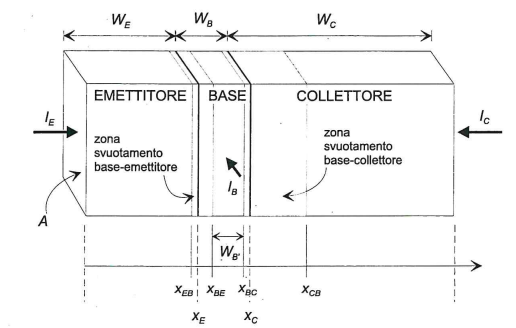
\includegraphics[width=0.5\textwidth]{Immagini_Micro&Nano/Imm_3_Transistor_BJT/npn monodimensionale.png}
    \caption{Caption}%
    \label{fig:enter-label}
\end{figure}\\
La giunzione base collettore influisce debolmente sulla corrente di collettore attraverso l'effetto Early  ma la cosa più importante è che stabilisce la tensione di breakdown del transistore in regione attiva diretta.\\
Il collettore è caratterizzato da una lunghezza $W_C$ e dal drogaggio $N_{DC}$ (in un transistore npn). La lughezza $W_C$ non  influenza le caratteristiche del BJT in regione attiva diretta e normalmente è più lungo rispetto alla base ed all'emettitore per necessità tecnologiche. 
Il motivo dietro la prima affermazione si spiega dal fatto che il collettore ha come unico scopo quello di raccoglie elettroni (portatori maggioritari) provenienti dalla base, e questo processo non involve la lunghezza del collettore (in realtà SI, ma in modo estremamanete trascurabile). Inoltre, la lunghezza del collettore viene presa grande perchè influisce sulle prestazioni del transistor al di fuori della RAD, come velocità di commutazione e guadagno di corrente.\\
Il drogaggio del collettore ha influenza sulle proprietà di breakdown del transistor . La giunzione base-collettore, polarizzata inversamente, presenta due meccanismi di breakdown, la perforazione diretta e il breakdown a valanga.
\subsubsection{Breakdown del BJT: perforazione diretta}
La perforazione diretta è causata dal fatto che la regione di svuotamento della giunzione B-C si allarga al crescere della polarizzazione inversa, ossia di $|V_{BC}|$, fino a raggiungere il punto di rottura.\\
Prima di continuare definisco alcuni parametri:
$\xi_B = x_C-x_{BC}$ è la profondità della regione di svuotamento della giunzione $B_C$ dal lato della base.\\
$\xi_C = x_{CB}-x_{C}$ è la profondità della regione di svuotamento della giunzione $B_C$ dal lato del collettore.\\
Ti ricordi i doscorsi fatti con la regione pn? aumentando la tensione inversa la regione di svuotamento aumenta in maniera proporzionale fino a quando non si ha perforazione, il BJT è uguale:
La perforazione diretta avviene quando $\xi_B \approx W_B$,

ossia quando la regione di svuotamento della regione B-C sì estende sull'intera base (si è trascurato lo spessore della regione E-B dal alto della base). \\
Per base e collettore drogati uniformemente sì ha:
\begin{align}
    \xi_C=\sqrt{\dfrac{2\varepsilon N_{eq}(V_{bi}-V_{BC})}{qN_{DC}^2}}\nonumber\\
    \xi_B=\sqrt{\dfrac{2\varepsilon N_{eq}(V_{bi}-V_{BC})}{qN_{AB}^2}} \nonumber
\end{align}
Dove $\frac{1}{N_{eq}}=\frac{1}{N_{DC}}+\frac{1}{N_{AB}}$ e $V_{bi}$ è la tensione di built-in.\\
Facendo il rapporto dei due si arriva alla formula:
\begin{equation}
    \dfrac{\xi_B}{\xi_C}=\dfrac{N_{DC}}{N_{AB}}
\end{equation}
Poichè la base è molto più sottile del collettore, è necessario fare in modo che il rapporto $\xi_B \ll \xi_C$ sia anch'esso piccolo in modo da evitare la perforazione ($\xi_B \approx W_B$) ossia, per mantenere il campo elettrico nella base basso e prevenire che i portatori di carica assumino  energia in base sufficiente alla perforazione. \\Questa situazione si può ottenere aumentando il drogaggio della base rispetto a quella del collettore:  
\begin{equation}
    N_{AB} \gg N_{DC}
\end{equation}
in definitiva, in un transistor bipolare il drogaggio deve decrescere dall'emettitore alla base al collettore. In queste condizioni $\xi_B=\sqrt{\frac{2\varepsilon N_{DC}(V_{bi}-V_{BC})}{qN_{AB}^2}}$ diventa trascurabile al punto tale da poter approssimare la regione di svuotamento B-C come se fosse data dalla sola $\xi_C=\sqrt{\frac{2\varepsilon N_{DC}(V_{bi}-V_{BC})}{qN_{DC}^2}}$.\\
\subsubsection{Breakdown del BJT: effetto valanga}
Il breakdown a valanga può avvenire in corrispondenza della giunzione base-collettore per polarizzazioni inverse elevate cioè per tensioni  $|V_{BC}|$ oltre la quale il campo elettrico $\mathcal{E}=\sqrt{\dfrac{2qN_{DC}(V_{bi}-V_{BC})}{\varepsilon}}$ raggiunge il valore di soglia per l'innesco della moltiplicazione a valanga. Per rendere minimo $\mathcal{E}$ sì può diminuire il drogaggio del collettore $N_{DC}$. ma è importante sapere che valori troppo bassi di $N_{DC}$ non sono opportuni perché aumentano la resistenza parassita del collettore.  



\section{26.10.2023}
\subsection{Elementi di non idealità}
Il primo elemento di non idealità è che $V_{CE}=V_{CB}+V_{BE}$
\begin{figure}[hbt!]
    \centering
    \begin{circuitikz}
        \draw(0,0)node[left]{B}--++(0.5,0) node[npn,anchor=B](npn){};
        \draw(npn.C)--++(0,0.5)node[above]{C};
        \draw(npn.E)--++(0,-0.5)node[below]{E};
        %Vbc
        \draw[red,-latex] (0.95,0.85) arc (90:180:0.75)node[above]{$V_{BC}$};
        \draw[red,-latex] (0.95,-0.85) arc (270:180:0.75)node[below]{$V_{BE}$};
        \draw[red,-latex] (1.45,-0.5) arc (270:360+90:0.5)node[above]{$V_{BC}$};
    \end{circuitikz}
    \caption{Caption}
    \label{fig:enter-label}
\end{figure}
%
\begin{ricevimento}
    sistemare
\end{ricevimento}

Se $V_{CE}$ aumenta e $VBE \approx V_{th}$, per fare in modo che il dispositivo rimanga attivo (E-B on) e continui ad erogare corrente, $V_{CB}$ dovrà aumentare (ovvero $V_{BC}$ dovrà diventare sempre più negativo), polarizzando maggiormente la B-C in maniera inversa ed aumentando la regione di svuotamento. Per questo motivo la caratteristica tensione corrente nella configurazione emettitore comune ha la seguente forma:
\begin{figure}[hbt!]
    \centering
    
\includegraphics[width=0.15\textwidth,angle=90]{ImmaginiImmagini_Micro&Nano/Imm_3_Transistor_BJT/caratteristicaBJTRAD.png}
    \caption{Caption}%
    \label{fig:enter-label}
\end{figure}

finchè la $V_{CE}$ è bassa, la tensione $V_{BC}$ può essere positiva, così che abbiamo 2 giunzioni polarizzate che mandano la $I_{tot}$ a zero, perchè le due correnti di giunzione idealmente si cancellano.\\
Quando non vi è più compensazione, il diodo non eragà più corrente ma la raccoglie in modo che Itot=cost..
corrente totale dipende solo da Vbe.\\
Si avrà un valore di Ib(Vbe). la tensione chemanda sottosoglia la giunzione BC risulta uguale a circa 0.3V in quanto se $Vce \approx0.2V$ (con $V_{BE}\approx V_{th}$) allora $V_{BC}=0.3V $.\\
la corrente di base aumenta in quanto si ha una riduzione delle ricombinazioni
 
\subsubsection{Effetto Early}

In un primo momento ho considerato il transistor come fosse un componente ideale. Con tale approssimazione ho ottenuto che la corrente  di uscita in RAD ($I_C=I_B/\beta$) è costante al variare della tensione $V_{CE}$ e quindi che il BJT si comporti come un generatore ideale di corrente pilotato dalla sola $I_B$.
Nella realtà  tuttavia, i BJT che operano in RAD hanno una corrente $I_C$ dipendente dalla tensione di uscita ($V_{BC}$ o $V_{CE}$) poichè queste ultime influenzano le dimensioni delle regioni di svuotamento, le quali modificano le correnti.\\

\begin{figure}[hbt!]
    \centering
    \begin{tikzpicture}
        \draw(0,0)--++(12,0);
         %disegno Xe
        \draw[densely dashed](4,0)--++(0,3);
        \draw[>=latex, <-,blue] (4,-0.1)--++(0,-0.5) node [anchor=north,blue]{$x_E$};
         %disegno Xbe
        \draw[densely dashed](4.5,0)--++(0,3);
        \draw[>=latex, <-,blue] (4.5,-0.1)--++(0,-0.3) node [anchor=north,blue]{$x_{BE}$};
         %disegno Xbc
        \draw[densely dashed](8.5,0)--++(0,3);
        \draw[>=latex, <-,blue] (8.5,-0.1)--++(0,-0.3) node [anchor=north,blue]{$x_{BC}$};
        \draw[>=latex, <-,blue] (7.5,-0.1)--++(0,-0.2) node [anchor=north,blue]{$x_{BC}'$};
         %disegno Xc
        \draw[densely dashed](9.5,0)--++(0,3);
        \draw[>=latex, <-,blue] (9.5,-0.1)--++(0,-0.5) node [anchor=north,blue]{$x_{C}$};
        
        \draw[dashed](0,0.5)--++(4,0);
        \draw[dashed](4,0.5)--++(4,0);
        \draw[dashed](8,0.5)--++(4,0)node[right]{$n_i^2$};
        
        \node at (2,3.5)[]{N};
        \node at (6,3.5)[]{P};
        \node at (10,3.5)[]{N};
        \node at (5.5,1.25)[]{$Q_B$};

        \draw[|-|](4.5,-2+0.5)--(8.5,-2+0.5);
        \draw(4.5+2,-1.8)node[]{$W_B$};
        
        \draw[|-|](4.5,-1)--(7.5,-1);
        \draw(4.5+1.5,-0.8)node[]{$W_B'$};
        %grafico rosso    
        \draw[very thick,red] (4.5,2.5)node[right,black]{$n_0$}-- (8.5,0.5);

        %carica
         \draw[pattern=north east lines, pattern color = red] (4.5,0.5)--(4.5,2.5)--(7.5,0.5)--(4.5,0.5);
               
    \end{tikzpicture}
    \caption{Caption}
    \label{fig:enter-label}
\end{figure}
%
Nel caso ideale le regioni di svuotamento sono state sempre di dimensione fissa e quindi anche la base ha sempre avuto larghezza costante $W_B$ indipendentemente dalle tensioni applicate.\\
In realtà lo spessore della base dipende, in regione attiva diretta, dalla tensione applicata alla base perchè al crescere della tensione di polarizzazione (all'aumentare di $V_{CE}$ si modifica $V_{Cb}$ quindi:) la base si assottiglia ($W_B' =W_B- \xi(V_{BC}) \ll W_B$) causando due effetti:
\begin{enumerate}
    \item La corrente emettitore (collettore) aumenta perchè si ha un eccesso della concentrazione dei portatori minoritari base. Graficamente questo corrisponde ad una pendenza della retta maggiore(vedere figura sopra).
\begin{exbox}
    nell'equazione che descrive $I_C$ c'è una dipendenza con Wb/Lnb nella spiegazione del Ghione, prima dell'eq (\ref{eq:Ebers-Mole})
    \begin{center}
        
\includegraphics[width=0.5\textwidth]{Immagini/imm23.10.2023/effetto Early.png}
    \end{center}
\end{exbox}
    Poichè la base è più drogata del collettore la variazione della $W_B$ dovuta alla $V_{BC}$ è resa minima, ma non annullata. Rendere minima questa variazione è una ulteriore ragione per drogare la base più del collettore. 
    \item La corrente di base\_diminuisce perché, diminuendo lo spessore della base, diminuisce  la ricombinazione dei portatori iniettati dall'emettitore con portatori maggioritari nella base. In altri termini, all'aumentare della polarizzazione inversa base-collettore diminuisce il tempo di transito e aumenta $\beta$. Pertanto, se si mantiene costante la corrente di base, la corrente di collettore aumenta ulteriormente.  \\
\end{enumerate}
%
\cleardoublepage
Il punto numero 2 si può studiare in pochi passaggi:\\
%
\begin{minipage}{0.45\textwidth}
    Parto dalla figura dei portatori minoritari all'interno della base comprese le regioni di svuotamento , poi ne considero l'approssimazione lineare.
    
    Il tempo si transito si può calcolare a aprtire di $Q_B$.
    La carica $Q_B$ è l'integrale della distribuzione di carica presenza nella giunzione di base (che abbiamo approssimato come lineare)
    %
    \begin{equation}
        \tau_t=\dfrac{Q}{I_C}
    \end{equation}
    %
    \begin{align}
        I_C &\approx D_n \dfrac{n_0}{W_B}\\
        Q_B&=\dfrac{n_0 W_B}{2}\\
        \tau_t&=\dfrac{1}{2} \dfrac{W_B^2}{D_n}
    \end{align}
    %
\end{minipage}
\hfill%
\begin{minipage}{0.45\textwidth}
    \begin{tikzpicture}[scale=0.65]
        \draw(0,0)--++(12,0);
         %disegno Xe
        \draw[densely dashed](4,0)--++(0,3);
        
         %disegno Xbe
        \draw[densely dashed](4.5,0)--++(0,3);
        
         %disegno Xbc
        \draw[densely dashed](8.5,0)--++(0,3);
        
         %disegno Xc
        \draw[densely dashed](9.5,0)--++(0,3);
       
        
        \draw[dashed](0,0.5)--++(4,0);
        \draw[dashed](4,0.5)--++(4,0);
        \draw[dashed](8,0.5)--++(4,0);

        \node at (2,3.5)[]{N};
        \node at (6,3.5)[]{P};
        \node at (10,3.5)[]{N};

        %grafico rosso
        \draw[very thick,red] (4,2.5) to [out=240,in=1] (0,0.55) ;
        \draw[very thick,red] (4.5,2.5).. controls (5.5,1.5) and (6.2,1.55) .. (6.5,1.45);
        \draw[very thick,red] (6.5,1.45) to [out=-5,in=120] (8.5,0) ;
        \draw[very thick,red] (9.5,0) to [out=20,in=180] (12,0.45) ;

        %tratteggi

        % grafico carica
         \draw[pattern=north east lines, pattern color = gray] (4.5,0)--(4.5,2.5).. controls (5.5,1.5) and (6.2,1.55) .. (6.5,1.45)to [out=-5,in=120] (8.5,0)--(4.5,0);

          \begin{scope}[shift={(0,-4)}]
          
            \draw(0,0)--++(12,0);
             %disegno Xe
            \draw[densely dashed](4,0)--++(0,3);
            \draw[>=latex, <-,blue] (4,-0.1)--++(0,-0.5) node [anchor=north,blue]{$x_E$};
             %disegno Xbe
            \draw[densely dashed](4.5,0)--++(0,3);
            \draw[>=latex, <-,blue] (4.5,-0.1)--++(0,-0.3) node [anchor=north,blue]{$x_{BE}$};
             %disegno Xbc
            \draw[densely dashed](8.5,0)--++(0,3);
            \draw[>=latex, <-,blue] (8.5,-0.1)--++(0,-0.3) node [anchor=north,blue]{$x_{BC}$};
            \draw[>=latex, <-,blue] (7.5,-0.1)--++(0,-0.2) node [anchor=north,blue]{$x_{BC}'$};
             %disegno Xc
            \draw[densely dashed](9.5,0)--++(0,3);
            \draw[>=latex, <-,blue] (9.5,-0.1)--++(0,-0.5) node [anchor=north,blue]{$x_{C}$};
            
            \draw[dashed](0,0.5)--++(4,0);
            \draw[dashed](4,0.5)--++(4,0);
            \draw[dashed](8,0.5)--++(4,0)node[right]{$n_i^2$};
            
            \node at (5.5,1.25)[]{$Q_B$};
    
            \draw[|-|](4.5,-2)--(8.5,-2);
            \draw(4.5+2,-1.8-0.5)node[]{$W_B$};
            
            \draw[|-|](4.5,-1-0.5)--(7.5,-1-0.5);
            \draw(4.5+1.5,-0.8-0.3)node[]{$W_B'$};
            %grafico rosso    
            \draw[very thick,red] (4.5,2.5)node[right,black]{$n_0$}-- (8.5,0.5);
    
            %carica
             \draw[pattern=north east lines, pattern color = red] (4.5,0.5)--(4.5,2.5)--(7.5,0.5)--(4.5,0.5);
          \end{scope}
    \end{tikzpicture}
\end{minipage}
\vspace{3mm}
%
Si capisce quindi che il tempo di transito diminuisce in modo proporzionale al quadrato di $W_B$ e ,dato che $\beta = \frac{\tau_0}{\tau_t}$ , si avrà un aumento del guadagno.\\
%
Se guardo il transistor dal punto di vista del collettore a modo comune:
\begin{center}
    
\includegraphics[width=0.15\textwidth,angle=90]{Immagini/imm23.10.2023/circuitoEarly.jpg}
\end{center}
Senza la $r_{ce}$, colui che produce il suddetto effetto early, si avrebbe un generatore di corrente perfetto
La pendenza implica l'esistenza della reisstenza, che vale in regime dinamico e NOn statico.
\subsubsection{Effetti di basso ed alto livello di iniezione, il diagramma di Gummel}
\begin{exbox}
    Gli effetti dovuti agli alti livelli di iniezioni si studieranno alla fine del corso. anche se non farà parte dell'argomento BJT, la teoria fisica è la stessa.
\end{exbox}
Per spiegare questa non idealità si fà ricorso al diagramma di Gummel. Sì tratta di un grafico in scala semilogaritmica della corrente di collettore e della corrente di base, in funzione della tensione $V_{BE}$, per valori tali da polarizzare direttamente la giunzione base-emettitore, e per un valore costante della tensione $V_{BC}$ tale da polarizzare inversamente la giunzione base-collettore.  Il valore di  $V_{BC}$ è poco importante, a meno che il transistore non presenti un effetto Early anormalmente elevato. 
\begin{figure}[hbt!]
    \centering
    
\includegraphics[width=0.5\textwidth]{Immagini/imm23.10.2023/gummel ideale.png}
    \caption{Caption}
    \label{fig:enter-label}
\end{figure}
Poiché in zona attiva diretta la dipendenza della corrente di base $I_B$ dalla tensione $V_{BE}$ segue idealmente la legge della giunzione pn ($I_B \approx I_0 \cdot \left[e^{V_{BE}/V_T}-1 \right]$), in scala semilogaritmica la curva $I_B(V_{BE})$ è approssimativamente una retta
Ma in regione attiva diretta $I_C \approx \beta I_B$, per cui anche $I_C(V_{BE})$ è una retta in scala semilogaritmica, spostata verso l'alto di $\log_{10}(\beta)$. Un esempio di Gummel plot ricavato dal modello ideale (teoria di Shockley) è mostrato nella figura sopra.\\

In un dispositivo ideale l'amplificazione $\beta$ in regione attiva diretta si mantiene costante per qualsiasi valore di corrente $I_B$ e $I_C$ (basse o alte che siano). Questo non avviene in pratica: in un transistore reale $\beta$ ha un massimo in un campo intermedio di tensioni ma decresce per bassa tensione (basse correnti) e per alte tensioni (alte correnti), come mostrato in Figura:
\begin{figure}[bht!]
    \centering
    
\includegraphics[width=0.5\textwidth]{Immagini/imm23.10.2023/andamento di beta.png}
    \caption{Caption}
    \label{fig:enter-label}
\end{figure}
Il vero diagramma di gummel per un transistore reale risulta essere:
\begin{figure}[hbt!]
    \centering
    
\includegraphics[width=0.5\textwidth]{Immagini/imm23.10.2023/diagramma di gummel.png}
    \caption{Caption}
    \label{fig:enter-label}
\end{figure}

Il diverso comportamento è da attribuirsi alle seguenti cause:  
\begin{enumerate}
    \item Per bassa $V_{BE}$ (e quindi per bassi valori di $I_C$) la corrente di collettore si comporta come $exp(V_{BE}/\eta V_T)$ con fattore di idealità 1 unitario, ma la corrente  di base si comporta come $exp(V_{BE}/\eta V_T)$ con fattore di idealità $\eta >1$, come evidenziato dalla pendenza costante ma inferiore. Il diverso fattore di idealità (di solito prossimo a 2) per la corrente di base è attribuibile, analogamente a quanto visto nel diodo pn, all'effetto della generazione-ricombinazione nelle regioni di carica spaziale. Spesso si ha anche un rilevante effetto di generazione e ricombinazione superficiali. Chiaramente $\eta> 1$ per la corrente di base comporta l'incrocio delle caratteristiche di base e collettore a basse tensioni, ossia il fatto che $\beta$ diviene prima unitario e poi addirittura < 1 per basse tensioni base-emettitore.  
    \item Per alta $V_{BE}$ può divenire significativo l'effetto della resistenza parassita di base, posta in serie all'elettrodo di base intrinseco. Esattamente come accade in un diodo pn polarizzato direttamente, a valori elevati di polarizzazione diretta la tensione applicata cade prevalentemente sulle regioni resistive del diodo. Questo fenomeno giustifica il discostarsi delle caratteristiche dall'andamento rettilineo, ma non la diminuzione di $\beta$.
    \item   Indipendentemente dall'effetto della resistenza parassita di base, per valori elevati di $V_{BE}$ (e quindi per valori elevati di $I_C$) $\beta$ decresce per un insieme di effetti di alta iniezione. ‘Tali effetti sono causati, in una giunzione pn polarizzata direttamente, dal fatto che i portatori minoritari in eccesso iniettati ai due lati della giunzione non sono più trascurabili rispetto ai portatori maggioritari. Anche se i modelli sviluppati sono validi solo in condizioni di basso livello di iniezione, è possibile introdurre in modo qualitativo l'effetto dell'alto livello di iniezione tenendo presente che questo può riguardare sia la base sia il collettore. Si ha allora:  
\begin{enumerate}
    \item     Effetto di alto livello di iniezione nella base: per valori elevati della tensione base-emettitore (transistore npn) la concentrazione degli elettroni  in eccesso iniettati nella base diviene paragonabile con la concentrazione delle lacune maggioritarie nella base. Poiché la base resta, almeno approssimativamente, neutrale, un aumento della concentrazione degli elettroni iniettati oltre il drogaggio della base comporta, per mantenere la neutralità della base, un accumulo di lacune, ossia un aumento del drogaggio equivalente della base. Ma un aumento del drogaggio della base produce una diminuzione dell'efficienza di emettitore, in quanto le lacune in eccesso nella base tenderanno a essere iniettate all'indietro nell'emettitore. Pertanto l'alto livello di iniezione nella base comporta una riduzione dell'amplificazione causata da una ridotta efficienza di emettitore.  
    \item Effetto di alto livello di iniezione nel collettore, detto anche effetto Kirk: come già osservato, ad alta corrente di collettore sì ha forte iniezione di elettroni dall'emettitore alla base (transistore npn), con conseguente richiamo di lacune in eccesso e aumento di drogaggio equivalente nella base. Tale aumento produce un restringimento della regione di carica spaziale base-collettore. Inoltre gli elettroni iniettati nel collettore, che per semplicità si suppone viaggino alla velocità di saturazione nella regione di alto campo base-collettore, schermano parzialmente i donatori ionizzati della regione di carica spaziale tra base e collettore, lato collettore. È quindi come se il drogaggio equivalente del collettore diminuisse. Nel complesso quindi il limite elettrico della base si sposta in avanti verso il collettore, mentre il limite elettrico del collettore neutro si sposta verso il contatto ohmico di collettore (spesso realizzato con un subcollettore $n^+$). L'allargamento della base quasi neutra (base pushout) implica l'aumento del tempo di transito e la diminuzione del $\beta$ del transistore. Per livelli di iniezione estremamente elevata il limite della base oltrepassa $x_C$, ossia il collettore diviene una regione quasi-neutrale con drogaggio trascurabile rispetto alla concentrazione degli elettroni in eccesso iniettati e delle lacune in eccesso che le compensano; in queste condizioni il collettore siì comporta a tutti gli effetti come una regione di tipo p, dando così luogo all'estensione della base fino al limite della regione di subcollettore $n^+$.  
\end{enumerate}
\end{enumerate}
%


\cleardoublepage
\section{BJT: comportamento dinamico}
Vogliamo introdurre un modello matematico del BJT ed un insieme di circuiti equivalenti validi in condizioni di polarizzazione arbitrarie
\subsection{Modello di Ebers-Moll}
Avevo trovato delle espressioni analitiche per le correnti $I_E$ ed $I_C$. Ora le riscrivo nella forma di Ebers-Moll e prenderanno il nome di equazioni di Ebers-Moll pilotate in tensione:
\begin{align}
    I_E&=\mathnormal{a}_{11} \left[ e^{V_{BE}/V_T} -1 \right] +\mathnormal{a}_{12} \left[ e^{V_{BC}/V_T} -1 \right]\\
    I_C&=\mathnormal{a}_{21} \left[ e^{V_{BE}/V_T} -1 \right] +\mathnormal{a}_{22} \left[ e^{V_{BC}/V_T} -1 \right]
\end{align}
Usando queste due equazioni sarò in grado di creare diversi circuiti equivalenti.
\begin{citbox}
    Dove i parametri $\mathnormal{a}_{ij}$[Ampere] assumono una certa equazione solo a assumento transistore a emettitore corto (?), drogaggio uniforme nelle tre regioni e con modello di Shockley. tali equazioni sono:
... pg 574
\end{citbox}

Per motivi spiegati più in dettaglio da Ghione, si avrà che
\begin{itemize}
    \item $a_{12}=a_{21}$
    \item $a_{11} \neq a_{22}$ perchè si considera l'approssimazione di drogaggio del collettore diverso da quello dell'emettitore.
    Sono prese diverse per mitigare il meccanismo che conduce all'effetto Early (riduzione di $W_B$ e conseguente aumento di $I_C$).
    Avremo la seguente situazione:
    \begin{center}
        \includegraphics[width=0.25\textwidth,angle=90]{Immagini/imm26.10.2023/drogaggioBJT.png}
    \end{center}
    Dove $N_{DE}>N_{AB}$ ènecessario per avere $\beta$ alto. $N_{AB}>N_{DC}$ mi garantisce minore variazione di $W_B$ in RAD perchè la regione di svuotamento si estenderà per lo più verso il collettore. Questa scelta, pur ducendo lo svuotamento in base provoca l'aumento della resistività.\\
    Per trovare un compromesso tra bassaresistività e contenimento dell'effetto early si realizza un primo tratto in cui $N_DC<N_{AB}$ e poi un bulck con $N_{DC}^B>N_{AB}$. cioè doppia diffusione .\\
    $\sigma=qN_D\mu_n$ e $\rho=1/\sigma$
\end{itemize}
Per individuare i valori di aij non si usano le formulazioni viste in precedenza, in quanto sperimentalemnte è complesso da studiare le costanti che compongono i parametri aij.
Per fare ciò passo al circuito equivalente di ebers mole.



\begin{citbox}[Come mai vale questa relazione?]
    questo valore non è casuale e vale per ogni transistore reale. Infatti per $V_{BE}\ll V_T, V_{BC}\ll V_T$ il transistore è prossimo all'equilibrio termodinamico ed i termini esponenziali si possono linearizzare, conducendo all'approssimazione:
..
\end{citbox}
\subsubsection{Circuito equivalenti di ebers moll I}
Consideriamo un BJT npn in regione attiva diretta.\\
Ricordo che la corrente $I_C$ (Formula: \ref{eq:formula Ic ebers-moll}) può essere ricavata attraverso la manipolazione matematica del parametro "fattore di trasporto in base ($b$)" ed ha la forma:
\begin{equation}
    I_C=-\alpha_F I_E +I_{CB0}
\end{equation}
dove il pedice F indica la condizione di regione attiva diretta.
Poichè $I_{CB0}$ è la corrente di saurazione inversa della giunzione B-C, si può supporre che per tensioni arbitrarie applicate alla giunzione B-C si possa scrivere
\begin{equation}
    I_C = -\alpha_F I_E +I_{CB0}\left[ e^{V_{BC}/V_T} -1 \right]
\end{equation}
Analoga situazione in regione attiva inversa:

\begin{equation}
    I_E=-\alpha_R I_C +I_{EB0}
\end{equation}
dove $I_{EB0}$ è la corrente di saturazione inversa della giunzione base-emettitore,
polarizzata inversamente in regione attiva inversa. In generale si potrà allora
scrivere: 
\begin{equation}
    I_E = -\alpha_R I_C +I_{EB0}\left[ e^{V_{BE}/V_T} -1 \right]
\end{equation}
Guardando queste equazioni dal punto di vista circuitale, vediamo che richiamano la seconda legge di Khirchoff, la legge dei Nodi, dove $I_{CB0}\left[ e^{V_{BC}/V_T} -1 \right]$ ed $I_{EB0}\left[ e^{V_{BE}/V_T} -1 \right]
$
sono le correnti dei diodi ideali pilotati dalle tensioni $V_{BE}$ e $V_{BC}$ mentre i termini $-\alpha_R I_C$ e $-\alpha_F I_E$ corrispondono a due generatori di corrente pilotati in corrente.\\
Da qui si ottiene il primo circuito equivalente di Ebers-Moll II:
\begin{figure}[hbt!]
    \centering
    \begin{tikzpicture}
        \draw (0,0) node[left]{E}
        to [short,*-]++(1,0)
        to [short]++(0,-0.75)
        to [D,invert]++(2,0)
        to [short]++(0,+0.75)
        to [short]++(1,0) coordinate(b)
        
        (b) to [short,*-*]++(0,-1.5)node[right]{B}
        
        (b) to [short]++(1,0)
        to [short]++(0,0.75)
        to [I, l^=$\alpha I_E$]++(2,0)
        to [short]++(0,-0.75)
        to [short,-*]++(1,0)node[right]{C};
    \end{tikzpicture}
    \caption{Caption}
    \label{fig:enter-label}
\end{figure}
\\%
%Dove le equazioni ai nodi sono:
%\begin{align}
 %   I_E &= \alpha_R I_C +I_{EB0}\left[ e^{V_{BE}/V_T} -1 \right]\\
  %  I_C &= \alpha_F I_E +I_{EB0}\left[ e^{V_{BC}/V_T} -1 \right]
%\end{align}
Sapendo che il BJT tecnologicamente è pressochè simmetrico, a meno di un differente drogaggio, il circuito equivalente finale risulterà essere :
%
\begin{figure}[hbt!]
    \centering
    \begin{tikzpicture}
        \draw (0,0) node[left]{E}
        to [short,*-]++(1,0)
        to [short]++(0,-0.75)
        to [D,invert]++(2,0)
        to [short]++(0,+0.75)
        to [short]++(1,0) coordinate(b)
        
        (b) to [short,*-*]++(0,-1.5)node[below]{B}
        
        (b) to [short]++(1,0)
        to [short]++(0,0.75)
        to [I, l^=$\alpha_F I_E$]++(2,0)
        to [short]++(0,-0.75)
        to [short,-*]++(1,0)node[right]{C};

        \draw (0,0)
        to [short,*-*]++(1,0)
        to [short]++(0,+0.75)
        to [I, l^=$\alpha_R I_C$,invert]++(2,0)
        to [short,-*]++(0,-0.75)
        to (b)
                
        (b) to [short,-*]++(1,0)
        to [short]++(0,-0.75)
        to [D]++(2,0)
        to [short,-*]++(0,+0.75)
        to [short,-*]++(1,0)node[right]{C};

        %labels
        \draw[-latex] (8,-0.25) --++ (-0.75,0)node[midway, below] {$I_C$}; %Ic
        \draw[-latex] (4.25,-1.25) --++ (0,1)node[midway, right] {$I_B$}; %Ib
        \draw[-latex] (0,-0.25) --++ (0.75,0)node[midway, below] {$I_E$}; %Ie

        %corrente diodi
        \draw[-latex] (1.5,-1.25) --++ (+1,0)node[midway, below] {$I_{EB0}\left[e^{{V_{BE}}/{V_T}}-1\right]$}; %Idc

        \draw[-latex] (8-1.5,-1.25) --++ (-1,0)node[midway, below] {$I_{CB0}\left[e^{{V_{BC}}/{V_T}}-1\right]$}; %Idc
        ;
    \end{tikzpicture}
    \caption{Caption}
    \label{fig:enter-label}
\end{figure}
%
\cleardoublepage
\subsubsection{Circuito equivalente di Ebers-Moll II o a iniezione}
Cambiano pilotaggio dei generatori dipendenti, facendo in modo che siano pilotati dalle correnti dei diodi invece dalle correnti di ingresso.\\
riscriviamo le equazioni come:
\begin{align}
    I_E &= -\dfrac{I_{EB0}}{1-\alpha_R \alpha_F}  \cdot \left[ e^{V_{BE}/V_T} -1 \right] 
        +\dfrac{\alpha_R I_{CB0}}{1-\alpha_R \alpha_F} \cdot \left[ e^{V_{BE}/V_T} -1 \right]\\
    I_C &= +\dfrac{\alpha_F I_{EB0}}{1-\alpha_R \alpha_F} \cdot \left[ e^{V_{BC}/V_T} -1 \right]
        -\dfrac{I_{CB0}}{1-\alpha_R \alpha_F}  \cdot \left[ e^{V_{BC}/V_T} -1 \right] 
\end{align}
%
\begin{exbox}
    Precedentemente ho visto come variano le relazioni a connettore comeune tra collettore e VCE:
\end{exbox}
%
Ponendo:
\begin{align}
    \dfrac{I_{EB0}}{1-\alpha_R \alpha_F}  &= I_{E0}\\
    \dfrac{I_{CB0}}{1-\alpha_R \alpha_F}  &= I_{C0}
\end{align}
Si ottiene:
\begin{align}
    I_E &= - I_{E0}  \cdot \left[ e^{V_{BE}/V_T} -1 \right] +\alpha_R I_{C0} \cdot \left[ e^{V_{BE}/V_T} -1 \right]\\
    I_C &=  \alpha_F I_{E0} \cdot \left[ e^{V_{BC}/V_T} -1 \right] -I_{C0}  \cdot \left[ e^{V_{BC}/V_T} -1 \right] 
\end{align}
Dove vale al relazione $\alpha_R I_{C0}=\alpha_F I_{E0}$.\\
Di seguito la realizzazioen circuitale delle precedenti equazioni:
%

\begin{figure}[hbt!]
    \centering
    \begin{tikzpicture}
        \draw (0,0) node[left]{E}
        to [short,*-]++(1,0)
        to [short]++(0,-0.75)
        to [D,invert]++(2,0)
        to [short]++(0,+0.75)
        to [short]++(1,0) coordinate(b)
        
        (b) to [short,*-*]++(0,-1.5)node[below]{B}
        
        (b) to [short]++(1,0)
        to [short]++(0,0.75)
        to [I, l^=$\alpha_F I_{F} $,invert]++(2,0)
        to [short]++(0,-0.75)
        to [short,-*]++(1,0)node[right]{C};

        \draw (0,0)
        to [short,*-*]++(1,0)
        to [short]++(0,+0.75)
        to [I, l^=$\alpha_R I_R$]++(2,0)
        to [short,-*]++(0,-0.75)
        to (b)
                
        (b) to [short,-*]++(1,0)
        to [short]++(0,-0.75)
        to [D]++(2,0)
        to [short,-*]++(0,+0.75)
        to [short,-*]++(1,0)node[right]{C};

        %labels
        \draw[-latex] (8,-0.25) --++ (-0.75,0)node[midway, below] {$I_C$}; %Ic
        \draw[-latex] (4.25,-1.25) --++ (0,1)node[midway, right] {$I_B$}; %Ib
        \draw[-latex] (0,-0.25) --++ (0.75,0)node[midway, below] {$I_E$}; %Ie

        %corrente diodi
        \draw[latex-] (1.25,-1.25) --++ (+1,0)node[midway, below] {$I_F=I_{E0}  \cdot \left[ e^{V_{BE}/V_T} -1 \right]$}; %Idc

        \draw[latex-] (8-1.25,-1.25) --++ (-1,0)node[midway, below] {$I_R=I_{C0}  \cdot \left[ e^{V_{BC}/V_T}-1\right] $}; %Idc
        ;
    \end{tikzpicture}
    \caption{Caption}
    \label{fig:enter-label}
\end{figure}
%
\begin{figure}[hbt!]
    \centering
    \includegraphics[width=0.5\textwidth]{Immagini/imm26.10.2023/circuiti equivalenti ebers moll in tutte le config.png}
    \caption{Caption}
    \label{fig:enter-label}
\end{figure}
%
\begin{figure}[hbt!]
    \centering
    \begin{tikzpicture}[scale=1]
        % asse x
        \draw[-latex](-0.5,0)--(5,0);
        % asse y
        \draw[-latex](0,-0.5)--(0,2.5);
        
        \draw[-latex](-10,0)--(4,0.25);
        \draw[-latex](-10,0)--(4,0.75);
        \draw[-latex](-10,0)--(4,1.5);

        \draw[-latex] (0.18,0.7)--(-0.18,-0.7); 
        %disegno grafico V>0
        \draw[thick,cyan!80!blue](0,0) to [out=70,in=185] (0.15,0.19) -- (4,0.26);
        \draw[thick,cyan!80!blue](0,0)--(0.1,.325 )to [out=80,in=195] (0.35,0.55) -- (4,0.76);
        \draw[thick,cyan!80!blue](0,0)--(0.18,0.75 )to [out=80,in=190] (0.50,1.13) -- (4,1.5);

        %disegno grafico V<0
        \draw[thick,cyan!80!blue](0,0) to [out=255,in=0] (-0.18,-0.1) -- ++(-3,0);
        \draw[thick,cyan!80!blue](0,0) to [out=255,in=0] (-0.17,-0.2) -- ++(-3,0);
        \draw[thick,cyan!80!blue](0,0) to [out=255,in=0] (-0.17,-0.3) -- ++(-3,0);
        %\draw[thick,cyan!80!blue](0,0) to [out=270,in=-185] (-0.15,-0.1) -- ++(-4,0);
        
    \end{tikzpicture}   
    \caption{Caption}
    \label{fig:enter-label}
\end{figure}
%
\subsection{Caratteristiche statiche}
Usando il modello circuitale di Ebers-Moll posso andare studiare le caratteristiche ideali e reali di un BJT (npn).
\subsubsection{Caratteristiche statiche ideali}
FIG\\
\\
QUando entrambe le giunzioni sono polarizzate direttamente ($V_{BC}>|V_{th}|, V_{BE}>V_{th}$) si hanno due correnti opposte che si cancellano. Man mano che la tensione di collettore aumenta, B-C và in OFF, invertendosi, realizzando lo scivolo energetico visto nel diagramma abande.\\
\begin{equation}
    \dfrac{I_B}{I_C}=\beta=\dfrac{\alpha_F}{1-\alpha_F}\approx 100 \ , \text{se }\ \alpha_F=0.99
\end{equation}
Se volessi lavorare in una condizione reverse, il comportamento è analogo ma a causa di $\alpha_R$ molto basso a causa della differenza dei drogaggi
%
\begin{equation}
    \beta^{REV}=\dfrac{D_n}{D_p}\cdot \dfrac{N_{DC}}{N_{AB}}\dfrac{W_C}{W_B} \ \text{con }\ N_{DC}\gg N_{AB}
\end{equation}
%
\subsubsection{Configurazione common base}
Andamento della corrente Ic in uscita in funzione della Ie in ingresso.
FIG\\
\\

\subsubsection{Caratteristiche statiche reali}
La più grande differenza dal mondo ideale è le equazioni di Ebers-Moll non descrivono due effetti dovuti alla non idealità dei componenti: il breakdown e l'effetto Early. Questi verranno spiegati nelle successive sezioni.
\paragraph{Polarizzazione del transistor bipolare}\mbox{}\\
pg587
%
\cleardoublepage 

\subsection{Modello del BJT per piccoli segnali}
In condizioni di piccolo segnale il transistore è eccitato da un generatore tempo-variante (di solito, sinusoidale) di ampiezza “piccola” rispetto alla polarizzazione in continua. In questo caso è possibile dividere le correnti e le tensioni  del
transistore, indicate con lettere minuscole e pedici maiuscoli, in una componente continua, indicata con lettera maiuscola, e in una componente alternata di piccolo segnale, indicata con lettera minuscola: 
\begin{align*}
    i_C(t)&= I_C + i_C(t)\\
    i_E(t)&= I_E + i_E(t)\\
    i_B(t)&= I_B + i_B(t)\\
    v_{BC}(t)&=V_{BC} + v_{BC}(t)\\
    v_{BE}(t)&=V_{BE} + v_{BE}(t)\\
    v_{CE}(t)&=V_{CE} + v_{CE}(t)
\end{align*}

pg 592--usare appunti pieraccini

\subsubsection{Circuito equivalente a $\pi$ di piccolo segnale }
%
Considero un BJT ad emettitore comune.\\
Se voglio rappresentare il circuito equivalente a $\pi$ devo prima calcolare gli elementi della matrice a conduttanze usando le equazioni di $I_E$ , $I_B$ ed $I_C$  statiche ad emettitore comune.
%
\begin{exbox}
    Si parte dalle caratteristiche a base comune (ottenute da ebers Mole II):
    \begin{align}
    I_E &= - I_{E0}  \cdot \left[ e^{V_{BE}/V_T} -1 \right] +\alpha_R I_{C0} \cdot \left[ e^{V_{BE}/V_T} -1 \right]\\
    I_C &=  \alpha_F I_{E0} \cdot \left[ e^{V_{BC}/V_T} -1 \right] -I_{C0}  \cdot \left[ e^{V_{BC}/V_T} -1 \right] 
\end{align}
%
e si pone $I_B=-I_E-I_C$, $V_{BC}=V_{BE}-V_{CE}$. Si ottiene:
%
\begin{align}
    I_B&=(1-\alpha_F)I_{E0}\left( e^{v_{BE}/V_T}-1\right)+(1-\alpha_R)I_{C0}\left(e^{v_{BE}/V_T}e^{-v_{CE}/V_T} -1\right) \\
     I_C&=\alpha_FI_{E0}\left( e^{v_{BE}/V_T}-1\right)-I_{C0}\left(e^{v_{BE}/V_T}e^{-v_{CE}/V_T} -1\right)
\end{align}
\end{exbox}
%
Gli elementi della matrice conduttanza saranno:
%
\begin{align}
    g_{BB} &= \left.\dfrac{di_B}{dv_{BE}}\right|_{V_{BE},V_{CE}}  &  g_{m} &= \left. \dfrac{di_C}{dv_{BE}}\right|_{V_{BE},V_{CE}} \\
    g_{BC} &= \left. \dfrac{di_B}{dv_{BC}}\right|_{V_{BE},V_{CE}}  & g_{CC} &= \left. \dfrac{di_B}{dv_{BC}}\right|_{V_{BE},V_{CE}} \nonumber
\end{align}
%
\begin{figure}[hbt!]
    \centering
    \begin{tikzpicture}
        \draw (0,-2) to [short,*-]++(0.01,0) node[left]{E} coordinate(e);
        \draw(0,0) node[above]{B} 
         to [short,*-*]++(1,0) coordinate(a)
         to [short]++(1.5,0) coordinate (f')
         to [open]++(1.5,0) coordinate (x)
         to [short,-*]++(2,0) coordinate (y)
         to [short,-*]++(1,0)node[above]{C}

         (a) to [R,l=$g_{BB}$,-*]++(0,-2) -| (e) 

         (f') to [I,-*]++(0,-2) node[below]{$g_{BC}$} -| (e) 
         (x) to [I,l=$g_mV_{BE}$,-*]++(0,-2)node[below]{$g_{m}$} -| (e) 
         
         (y) to [R,l=$g_{CC}$,-*]++(0,-2)  to [short,-*]++(1,0) -| (e) 
         ;
         
    \end{tikzpicture}
    \caption{Caption}
    \label{fig:enter-label}
\end{figure}
%
\begin{exbox}
    \begin{align}
    g_{BB} &= \left.\dfrac{di_B}{dv_{BE}}\right|_{V_{BE},V_{CE}} = \dfrac{(1-\alpha_F)I_{E0}}{V_T}e^{V_{BE}/V_T}-\dfrac{(1-\alpha_R)I_{C0}}{V_T}e^{V_{BE}/V_T}e^{-V_{CE}/V_T}\\
    g_{m} &= \left. \dfrac{di_C}{dv_{BE}}\right|_{V_{BE},V_{CE}}=-\dfrac{(1-\alpha_R)I_{C0}}{V_T}e^{V_{BE}/V_T}e^{-V_{CE}/V_T}\\ 
    g_{BC} &= \left. \dfrac{di_B}{dv_{BC}}\right|_{V_{BE},V_{CE}}= \dfrac{\alpha_F I_{E0}}{V_T}e^{V_{BE}/V_T}-\dfrac{\alpha_R I_{C0}}{V_T}e^{V_{BE}/V_T}e^{-V_{CE}/V_T}\\
    g_{CC} &= \left. \dfrac{di_B}{dv_{BC}}\right|_{V_{BE},V_{CE}}= \dfrac{I_{C0}}{V_T}e^{V_{BE}/V_T}e^{-V_{CE}/V_T}\\
\end{align}
Nella condizione di regione attiva diretta si applicano diverse semplificazioni dovute al fatto che $V_{BE}-V_{CE}=V_{BC}<0$. Allora
%
\begin{align}
    i_B &\approx (1-\alpha_F)I_{E0}e^{v_{BE}/V_T}\\
    i_C &\approx \alpha_F I_{E0}e^{v_{BE}/V_T}
\end{align}
%
A seguito di questa approssimazione si avrnno le correnti $i_B$ ed $i_C$ indipendenti alla tensione $v_{CE}$. Di conseguenza si dovrebbe ottenere $g_{BC}= g_{CC} = 0$ ma se voglio modellizzare il comportamento del BJT in modo che sia quanto più possibile fedele alla realtà (sempre sotto certe approssimazioni) dovrò considerare l'incremento della pendenza di $i_C$ dato dall'effetto Early.
Questo incremento di pendenza lo posso tenere in contro dentro i parametri $g_{BC}, g_{CC}$ tenendo presente che:
%
\begin{align}
    \dfrac{\Delta I_C}{\Delta V_{CE}} &\approx \dfrac{I_C}{V_{Early}}\\
    \Delta I_B &\approx -\dfrac{\Delta I_C}{\beta}
\end{align}
%
IMPORTANTE: il segno negativo dipende dal fatto che, mantenendo costante la tensione
base-emettitore, la corrente di base diminuisce a causa dell'effetto Early (perché
diminuisce la carica in eccesso nella base e quindi la ricombinazione nella base).

\begin{ripasso}[da elettronica generale]
    $V_{Early}$ è diverse decine di volt (raggiunge anche il centinaio), $i_B$ è dell'ordine del $\mu A$, $\beta$ è diverse centinaia (tipicamente 300) mentre $i_C$, seppur dipendente dal tipo di applicazione è, di solito, dell'ordine del ($m A$).\\
    Quindi $g_{BC}, g_{CC} \approx 0$ anche se, ripeto, $i_C$ potrebbe essere anche più grande, a seconda dell'applicazione.
\end{ripasso}
%
\end{exbox}
%
Si ottiene, nell'approssimazione di regione attiva diretta ($V_{BE} — V{CE} = V_{BC} < 0$):
%
\begin{equation}
    g_{BB} \approx \dfrac{I_B}{V_T}=\dfrac{I_C}{\beta V_T}
\end{equation}
%
\begin{equation}
    g_{BC} \approx \dfrac{I_B}{V_{Early}} = -\dfrac{I_C}{\beta V_{EARLY}} \approx 0
\end{equation}
%
\begin{equation}
    g_{CB}=g_{m} \approx \dfrac{I_C}{V_T} =\beta \dfrac{I_B}{V_{T}}
\end{equation}
%
\begin{equation}
    g_{CC} \approx \dfrac{I_C}{V_{Early}}
\end{equation}
%
Le equazioni precedenti possono essere utilizzate per definire gli elementi del circuito equivalente a $pi$ nella configurazione a emettitore comune.
Imponendo $|g_{BB}|\gg|g_{BC}|$,$|g_{CB}|\gg|g_{BC}|$,$|g_{CC}|\gg|g_{BC}|$, si avrà che: 
%
\begin{align}
    r_{BE}&=\dfrac{1}{g_{BB}+g_{BC}}\approx \dfrac{1}{g_{BB}}=\dfrac{V_T}{I_B}= \beta \dfrac{V_T}{I_C} \\
    r_{BC}&= \dfrac{1}{-g_{BC}}= \beta \dfrac{V_{Early}}{I_C} \\
    g_m &=g_{CB}-g_{BC}\approx \beta \dfrac{I_B}{V_T} \\
    r_{CE} &= \dfrac{1}{g_{CC}+g_{BC}}\approx \dfrac{1}{g_{CC}}= \dfrac{V_{Early}}{I_C} \\
\end{align}
%
Gli elementi $r_{BC}$ e $r_{CE}$ hanno valore elevato e possono essere spesso sostituiti da circuiti aperti.\\
Spesso il circuito equivalente a $\pi$ può essere modificato per tener
conto della resistenza parassita di base, aggiungendo la resistenza
serie parassita $r_{BB}$ all'incresso della base
%
\begin{figure}[hbt!]
    \centering
    \begin{tikzpicture}
        \draw (0,-2) to [short,*-]++(0.01,0) coordinate(e);
        \draw(0,0) node[above]{B} 
         to [R,l=$r_{BB'}$,*-*]++(2,0) coordinate(a)
         to [R,l=$r_{BC}$,-*]++(2,0) coordinate (x)
         to [short,-*]++(2,0) coordinate (y)
         to [short,-*]++(1,0)node[above]{C}

         (a) to [R,l=$r_{BE}$,-*]++(0,-2) -| (e) 

         (x) to [I,l=$g_mV_{BE}$,-*]++(0,-2) node[below]{E} -| (e) 
         
         (y) to [R,l=$r_{CE}$,-*]++(0,-2) to [short,-*]++(1,0) -| (e) 
         ;
         %label
         \draw[-latex] (-1,0) -- ++(0.75,0) node[midway, above] {$I_B$};
         \draw[latex-] (7.25,0)--++(+1,0) node[midway, above] {$I_C$};
         \draw[-latex] (0,-1.75)--++(0,1.5) node[midway, left] {$V_{BE}$};
         \draw[-latex] (7,-1.75)--++(0,1.5) node[midway, right] {$V_{CE}$};
    \end{tikzpicture}
    \caption{Caption}
    \label{fig:enter-label}
\end{figure}\\
%
Approssimando $r_{BC}$ come circuito aperto e inserendo $r_{BB'}$ dentro $r_{BE}$ si otterrebbe
%
\begin{figure}[hbt!]
    \centering
    \begin{tikzpicture}
        \draw (0,-2) to [short,*-]++(0.01,0) coordinate(e);
        \draw(0,0) node[above]{B} 
         to [short,*-]++(2,0) coordinate(a)
         to [open]++(2,0) coordinate (x)
         to [short,-*]++(2,0) coordinate (y)
         to [short,-*]++(1,0)node[above]{C}

         (a) to [R,l=$r_{BE}$,-*]++(0,-2) -| (e) 

         (x) to [I,l=$g_mV_{BE}$,-*]++(0,-2) node[below]{E} -| (e) 
         
         (y) to [R,l=$r_{CE}$,-*]++(0,-2) to [short,-*]++(1,0) -| (e) 
         ;
         %label
         \draw[-latex] (-1,0) -- ++(0.75,0) node[midway, above] {$I_B$};
         \draw[latex-] (7.25,0)--++(+1,0) node[midway, above] {$I_C$};
         \draw[-latex] (0,-1.75)--++(0,1.5) node[midway, left] {$V_{BE}$};
         \draw[-latex] (7,-1.75)--++(0,1.5) node[midway, right] {$V_{CE}$};
    \end{tikzpicture}
    \caption{Caption}
    \label{fig:enter-label}
\end{figure}
%
\begin{exbox}[perchè mi voglio male]
In un primo momento posso pensare di risolvere usando il teorema di miller, per "disaccoppiare" B e C, collegate da $R_{BC}$.
Definendo $K=\dfrac{V_{CE}}{V_{BE}}$ avrò a sinistra $Z'=\dfrac{Z}{1-K}$ ed a destra avrò $Z''=\dfrac{KZ}{K-1}$.\\
togliendo di mezzo la resistenza parassita di base $r_{BB'}$, avrò:
\begin{align*}
    V_{BE}&=I_B \cdot r_{BE}\\
    V_{CE}&=(I_C-g_mV_{BE})\cdot r_{CE}
\end{align*}
\begin{center}
    \begin{tikzpicture}
        \draw (0,-2) to [short,*-]++(0.01,0) coordinate(e);
        \draw(0,0) node[above]{B} 
         to [R,l=$r_{BB'}$,*-*]++(2,0) coordinate(a)
         to [short]++(1.5,0) coordinate (f')
         to [open]++(2,0) coordinate (f'')
         to [short]++(1.5,0) coordinate (x)
         to [short,-*]++(2,0) coordinate (y)
         to [short,-*]++(1,0)node[above]{C}

         (a) to [R,l=$r_{BE}$,-*]++(0,-2) -| (e) 

         (f') to [generic,l=$Z'$,-*]++(0,-2) -| (e) 
         (f'') to [generic,l=$Z''$,-*]++(0,-2) -| (e) 
         (x) to [I,l=$g_mV_{BE}$,-*]++(0,-2) node[below]{E} -| (e) 
         
         (y) to [R,l=$r_{CE}$,-*]++(0,-2) to [short,-*]++(1,0) -| (e) 
         ;
         %label
         \draw[-latex] (-1,0) -- ++(0.75,0) node[midway, above] {$I_B$};
         \draw[latex-] (7.25+3,0)--++(+1,0) node[midway, above] {$I_C$};
         \draw[-latex] (0,-1.75)--++(0,1.5) node[midway, left] {$V_{BE}$};
         \draw[-latex] (7+3,-1.75)--++(0,1.5) node[midway, right] {$V_{CE}$};
    \end{tikzpicture}
    \captionof{figure}{caption miller pi greco}
    \begin{citbox}
        continuare a risolvere da me
    \end{citbox}
\end{center} 
\end{exbox}


\cleardoublepage
\subsubsection{Comportamento in frequenza}
i modelli precedenti non contengono elementi reattivi anche se a ben pensarci, le giunzioni pn ed np si comportano un anche come delle capacità.
%
\begin{figure}[hbt!]
    \centering
    \begin{tikzpicture}
        \draw (0,-2) to [short,*-]++(0.01,0) coordinate(e);
        \draw(0,0) node[left]{B}
         to [short,*-]++(1,0) coordinate (Cbe)
         to [C,l=$C_{BE}$,*-*]++(0,-2) -| (e)

         (Cbe) to [short,-*]++(2,0) coordinate(a)
         to [R,l=$r_{BC}$,-*]++(2,0) coordinate (x)
         to [short,-*]++(2,0) coordinate (y)
         to [short,-*]++(1,0)node[right]{C}

         (a) to [R,l=$r_{BE}$,-*]++(0,-2) -| (e) 
         
         (a) to [short]++(0,1) 
         to [C,l=$C_{BC}$]++(2,0) to [short,-*]++(0,-1) 

         (x) to [I,l=$g_mv_{BE}$,-*]++(0,-2) node[below]{E} -| (e) 
         
         (y) to [R,l=$r_{CC}$,-*]++(0,-2) to [short,-*]++(1,0) -| (e) 
         ;
    \end{tikzpicture}
    \caption{Caption}
    \label{fig:enter-label}
\end{figure}
%
Le capacità sono trascurabili quando il segnale varia lentamente ma per applicazioni a Radiofrequenza è necessario studiarli perchè  non saranno più approssimabili come circuiti aperti ma avranno impedenza capacitiva molto piccola.\\
è necessario introdurre nel circuito a $\pi$ le capacità di giunzione che sono, in regione attiva diretta:
%
\begin{enumerate}
    \item Capacità B-E $C_{BE}$. Siccome la giunzione B-E è polarizzata direttamente, si tratta in prima approssimazione di una capacità di diffusione legata alla carica in eccesso accumulata nella base. (Se l'efficienza di emettitore è elevata, si può trascurare la componente capacitiva associata alla carica in eccesso iniettata dalla base nell'emettitore.) 
    Il calcolo di questa capacità non ha lo stesso risultato di quello nella giunzione pn perchè nel BJT la base è corta. \\Si può peraltro definire: 
    \begin{align}
        C_{BE} = \dfrac{dQ_B}{dV_{BE}} = \dfrac{dQ_B}{dI_C} \cdot \dfrac{dI_C}{dV_{BE}}
    \end{align}
    ma, tenendo presente la discussione sul tempo di transito in base ($\tau_t=\left|\frac{dQ_B}{dI_E}\right|$) e che \\ $\left|\frac{dI_E}{dV_{BE}}\right| \approx \left|\frac{dI_C}{dV_{BE}}\right| = g_m$, si ha :
    \begin{equation}
    C_{BE}= \textcolor{red}{\tau_t \cdot g_m} =\frac{\tau_t I_C}{V_T}=\frac{\tau_0 I_B}{V_T}
\end{equation}
    dove $\tau_0$ è la vita media dei portatori minoritari nella base, e si è utilizzata la definizione $\beta \approx \frac{\tau_0}{\tau_t}$. 

    \item Capacità base-collettore $C_{BC}$: poiché la relativa giunzione è polarizzata inversamente, si tratta di una capacità della regione di svuotamento (prevalentemente dal lato collettore, meno drogato), di solito molto bassa. 
\end{enumerate}

Il mio obiettivo è determinare la frequenza oltre il quale il dispositivo non è più utilizzabile secondo le specifiche. Infatti, a frequenze elevate le capacità base-emettitore e base-collettore tendono a cortocircuitare le rispettive giunzioni, e l'amplificazione del transistore si abbassa progressivamente. \\
Per determinare questo valore di frequenza, considero l'amplificazione di corrente di cortocircuito in funzione della frequenza.
\begin{exbox}[perchè si considera l'amplificazione di corrente di cortocircuito?]
    Perchè il mio scopo ultimo è ottenere un elevata corrente in uscita applicando in ingresso una certa $I_B$. Quando è che la corrente che scorre lungo un carico raggiunge il valore massimo? quando il carico è cortocircuitato! \\
    Quindi io voglio calcolare la frequenza massima nella condizione di massima corrente in uscita, cioè considerando un cortocircuito.
    \begin{ricevimento}
        chiedere se è giusto
    \end{ricevimento}
    
\end{exbox}
%
\paragraph{Calcolo del prodotto guadagno banda $f_T$}\mbox{}\\
\begin{figure}[hbt!]
    \centering
    \begin{tikzpicture}[scale=0.9, transform shape]
        \draw (0,-2) to [short,*-]++(0.01,0) coordinate(e);
        \draw(0,0) node[left]{B}
         to [short,*-]++(1,0) coordinate (Cbe)
         to [C,l=$C_{BE}$,*-*]++(0,-2) -| (e);

         \draw(Cbe) to [short,-*]++(2,0) coordinate(a)
         to [open,-*]++(2,0) coordinate (x)
         to [short,-*]++(2,0) coordinate (y);
         \draw(y) to [short,-*]++(1,0)node[above]{C} coordinate (c);

         \draw (a) to [R,l=$r_{BE}$,-*]++(0,-2) -| (e) ;
         
         \draw(a) to [short]++(0,1) 
         to [C,l=$C_{BC}$]++(2,0) to [short,-*]++(0,-1) ;

         \draw(x) to [I,l=$g_mv_{BE}$,-*]++(0,-2) node[below]{E} -| (e) ;
         
         \draw(y) to [R,l=$r_{CC}$,-*]++(0,-2) to [short,-*]++(1,0) -| (e) 
         ;
         \draw[color=red] (c)--++(0.5,0) to [short]++(0,-2)--++(-0.5,0);
    \end{tikzpicture}
    \caption{Caption}
    \label{fig:enter-label}
\end{figure}\\
%
Si parte considerando:
%
\begin{equation}
    V_{BE}=I_C \dfrac{I_B}{\dfrac{1}{r_{BE}}+j\omega (C_{BE}+C_{BC})}
\end{equation}
%
da cui ricavo $I_C=gm \cdot V_{BE}$, allora:
%
\begin{equation}
    \beta(\omega)=\dfrac{I_C}{I_B}=\dfrac{\beta}{1+j\dfrac{f}{f_{\beta}}}
\end{equation}
%
dove $f_{\beta}=\dfrac{1}{2\pi(C_{BE}+C_{BC})r_{BE}}$ è la frequenza di taglio a 3dB.
Da notare l'andamento di $\beta(f)$ decresce con l'aumento della frequenza:
\begin{itemize}
    \item Per $f<f_{\beta},\ |\beta(f)| \approx \beta$;
    \item Per $f \approx f_{\beta},\ |\beta(f)|=\beta/\sqrt{2}$;
    \item Per $f \gg f_{\beta},\ \beta(f)=-j\beta f_{\beta}/f$;
\end{itemize}
%
Ora definisco la frequenza di transito, meglio ricordato come prodotto guadagno banda, $f_T$ alla quale il modulo dell'amplificazione di corrente diventa unitario ($|\beta(f)|= 1 \approx \dfrac{\beta f_{\beta}}{f}$),nottenendo:
%
\begin{equation}
    f_T=\dfrac{\beta}{2\pi (C_{BE+C_{BC}})r_{BE}}=\textcolor{red}{\beta \cdot f_{\beta}}
\end{equation}
%
Ricordando che $\beta/r_{BE}=I_C/V_T=gm$ e ponendo $C=C_{BE}+C_{BC}$:
\begin{equation}
    f_T=\dfrac{g_m}{2\pi C}
\end{equation}
%
\cleardoublepage

\section*{30.10.2023}
Nei circuiti integrati digitali il transistore lavora solo in due regioni: saturazione (stato ON o livello logico 1) e interdizione (stato OFF o livello logico 0).\\
Bisogna considerare che i transistor commutano continuamente e che durante la variazione di stato il punto di lavoro
dinamico del transistore attraversa la regione attiva.\\
ricapitolando, il transistore:
%
\begin{itemize}
    \item utilizza, in condizioni stazionarie, le regioni di saturazione e interdizione
    \item utilizza, in condizioni dinamiche, la regione attiva diretta (serve per commutare)
\end{itemize}
%
\subsection{Transitorio di accensione (OFF-ON)}
%
\begin{figure}[hbt!]
    \centering
\begin{tikzpicture}[scale=0.45]
    %\node[anchor=south west,inner sep=0] (image) at (0,0) {
\includegraphics[width=0.9\textwidth]{ImmaginiBJT/provacarattbjt.PNG}};
   % \begin{scope}[x={(image.south east)},y={(image.north west)}]
     %   \draw[help lines,xstep=.1,ystep=.1] (0,0) grid (1,1);
     %   \foreach \x in {0,1,...,9} { \node [anchor=north] at (\x/10,0) {\x}; }
     %   \foreach \y in {0,1,...,9} { \node [anchor=east] at (0,\y/10) {\y}; }
   % \end{scope}
    %disegno assi cartesiani
    \draw[thick, -latex](0,0)--(14,0);
    \draw[thick, -latex](0,0)--(0,13);
    %disegno grafici
    \draw[thick, thick,cyan!80!blue](0,0)to [in=195, out=80](0.55,0.58)--(13,0.75);
    \draw[thick, thick,cyan!80!blue](0,0)--(0.48,2.5) to [in=195, out=80](0.84,2.84)--(13,3.4);
    \draw[thick, thick,cyan!80!blue](0,0)--(0.8,5.25) to [in=185, out=80](1.4,5.55)--(13,6.65);
    \draw[thick, thick,cyan!80!blue](0,0)--(1.1,7.9) to [in=185, out=80](2,8.3)--(13,9.45);
    \draw[thick, thick,cyan!80!blue](0,0)--(1.25,9.9) to [in=185, out=80](2.2,10.9)--(13,12.5);

    \draw[blue](13,0.75)..controls (13.75,0.75) and (13.9,6).. (13.95,7);
    \draw[blue](13,3.4)..controls (13.75,3.25) and (13.8,7).. (13.9,8);
    %
    \pgfmathsetseed{2}
     \draw(11.6,0)--+(0.1,0) coordinate (i);
     \foreach \i in {1,2,3,4,5} { 
    \draw[black,thick,, -latex] (i)  
      -- ++(-2.24,2.05) coordinate(i); 
    }
    \draw[black,thick,](11.7-2.24*5, 2.05*5)--(0,10.7);

    \draw[fill] (10.9,0.74) circle (0.13 cm);
    \draw[fill] (1.23,9.6) circle (0.13 cm);
\end{tikzpicture}
\end{figure}
%
Come visto in precedenza:
\begin{align}
    I_B &= \dfrac{Q_B}{\tau_0} \nonumber\\
    I_C &= \dfrac{Q_B}{\tau_T} \nonumber
\end{align}
%
dove $Q_B$ e è la carica in eccesso accumulata nella base e $\tau_0$ la vita media dei portatori minoritari nella base.
Da ricordare che che la base è quasi-neutra, per cui le popolazioni in eccesso di elettroni e lacune sono uguali.
Conosco inoltre:
%
\begin{equation}
    \beta=\dfrac{I_C}{I_B}=\dfrac{\tau_0}{\tau_T} \nonumber
\end{equation}
%
In condizioni dinamiche l'equazione $I_B$ può
essere estesa in modo da tener conto delle variazioni della carica in eccesso. \\
Si ottiene l'equazione di controllo di carica
%
\begin{equation}
    I_B(t) = \dfrac{Q_B}{\tau_0} + \dfrac{dQ_B(t)}{dt}
\end{equation}
%
Si consideri un BJT (ad emettitore comune) inizialmente OFF. \\
Entrambe le giunzioni sono
polarizzate inversamente e quindi non vi è carica in eccesso nella base; la corrente
di base è praticamente nulla.\\
Supponiamo che al tempo $t = 0$ la corrente di base sia portata da zero ad un valore $I_{B1}$ sufficiente a saturare il dispositivo. \\
La corrente $I_{B1}$ inietta nella base una popolazione di lacune in eccesso, che rendono la
base carica positivamente e abbassano la barriera base-emettitore richiamando così
elettroni dall'emettitore. \\
Dopo un brevissimo transitorio iniziale (che si esaurisce
in un tempo $t_{in}$ dell'ordine del tempo di transito) nel quale le cariche iniettate
diffondono nella base e danno luogo alla distribuzione lineare di carica tipica della
zona attiva, il transistore esce dalla zona di interdizione ed entra in zona attiva
diretta . Una volta in zona attiva diretta, la carica iniettata in
eccesso dal lato emettitore continua ad aumentare per compensare la carica in
eccesso iniettata dalla corrente di base; fino a che tale compensazione non ha
avuto luogo la barriera base-emettitore non può alzarsi nuovamente limitando il
flusso di cariche iniettate.
Il tempo t; necessario a stabilire nella base una carica in eccesso Q e alimentando il transistore con una corrente di base Ip, si valutà integrando la $I_B$;
Maneggiando $I_B$ trovo che

\begin{equation}
    \int_0^{Q_B} \dfrac{\tau_0 }{\tau_0 I_{B1}-Q_B'} dQ_B'= \int_0^t dt
\end{equation}
%
da cui:
%
\begin{equation}
    t=\tau_0 \cdot \log{\left[ \dfrac{\tau_0 I_{B1}}{\tau_0 I_{B1}-Q_B}\right]}
\end{equation}
%
Ora sono in grado di calcolare la carica $Q_B$ accumulata nel tempo $t$:
\begin{equation}
    Q_B= I_{B1} \cdot \tau_0 \cdot \left[ 1- e^{-\frac{t}{\tau_0}}\right]
\end{equation}
%
\begin{figure}[h]
    \centering
    \begin{tikzpicture}
        
    \end{tikzpicture}
    \caption{Caption}
    \label{fig:enter-label}
\end{figure}
%
Poiché la situazione che stò analizzando è dinamica, non è vero che la corrente di collettore
è proporzionale alla corrente di base attraverso il parametro $\beta$. \\
Peraltro prendendo la formula di $I_C$ riportata all'inizio, possiamo vedere come la carica iniettata nella base cresce, la corrente di collettore creace a sua volta nel tempo spostando il punto di lavoro dinamico del transistore lungo la retta di carico di uscita. Per corrente di collettore sufficientemente elevata la tensione
collettore-emettitore sì abbassa al punto da fare entrare il transistore nella zona
di saturazione. Chiamiamo $I_{cs}$ tale corrente di collettore e definiamo $t_S$ come il
tempo necessario a raggiungere l'innesco della saturazione, ossia $I_c = I_{cs}$. Si ha, tenendo presente che $Q_B=\tau_t I_C=\dfrac{\tau_0 I_C}{\beta}$:
\begin{equation}
    t_s = \tau_0 \log{\left[ \dfrac{\beta I_{B1}}{\beta I_{B1}-I_{CS}}\right] \tikzmark{a}} 
\end{equation}

L'equazione precedente fornisce il tempo necessario alla commutazione di
un transistore alimentato da una corrente di base $I_{B1}$, con tempo di vita medio
dei portatori in base $\tau_0$, e caricato in modo tale da richiedere, per la saturazione, una corrente di collettore $I_{CS}$. Detta $I_{BS} = I_{CS}/\beta$ la corrente di base DC
corrispondente alla polarizzazione di collettore $I_{CS}$, sì ha che: 

\begin{enumerate}
    \item Per $I_{B1}<I_{BS}$ non ha soluzioni reali, ossia la corrente di collettore
non raggiunge mai $I_{DS}$. Questo non è sorprendente, perché non è possibile
che il transistore, alimentato in condizioni stazionarie da $I_{B1} < I_{BS}$, presenti
una corrente di collettore $\beta I_{B1}=I_{CS}=\beta I_{BS}$.
\item Per $I_{B1} = I_{BS}$ il tempo di commutazione è infinito, ossia la corrente di base
è appena sufficiente a fornire la corrente di collettore voluta. 

\item Per $I_{B1} > I_{BS}$, ossia quando la corrente di pilotaggio è maggiore della corrente
statica necessaria a sostenere $I_{CS}$, il tempo di commutazione è finito e tanto
più breve quanto più è elevata $I_{B1}$. 
\end{enumerate}
Per ridurre il tempo di commutazione ci sono diverse strade:
\begin{enumerate}
    \item Rendere minimo il tempo di vita medio $\tau_0$. Questo effetto pùò essere ottenuto
drogando la base con sostanze opportune che fungono da centri di ricombinazione, ad esempio con Au. 
\item Aumentare l'amplificazione di corrente. Questa seconda condizione si oppone
peraltro alla prima, poiché $\beta$ è direttamente proporzionale alla vita media. Sì
osservi che i criteri di progetto di ùun transistore per commutazione coincidono, per quanto riguarda il $\beta$ elevato, con quelli di un transistore usato come
amplificatore. 

\item aumentare la corrente di pilotaggio:
\begin{equation}
    I_C=\dfrac{Q_B}{\tau_t}=\dfrac{I_{B1}\tau_0}{\tau_t}\left[ \-e^{-t/\tau_0}\right]
\end{equation}
per cui, a parità di altre condizioni, il valore di $I_{CS}$ è raggiunto tanto più
rapidamente quanto è più elevato $I_{B1}$. 
\end{enumerate}
............
Dal punto di vista esterno l'innesco della saturazione stabilizza il punto di lavoro
del transistore per alti valori di corrente di collettore e bassi valori della tensione collettore-emettitore. Tenendo presente che in saturazione $V_{CE} \approx 0$, per un
transistore alimentato da una batteria di valore $V_{CC}$ e con resistenza serie di emettitore $R_3$ 
\begin{figure}
    \centering
    \begin{circuitikz}
        \draw (0,0) node[npn,anchor=B](npn){};
        \draw(npn.E) --++(0,-1) to node[tlground]{}++(0,0);
        \draw(npn.C) to [R,l_=$R_3$]++(0,1.5)--++(-0.75,0) coordinate(V);
        \draw(V) to [short,-*]++(0,+0.5)node[right]{$V_{CC}$};
        \draw(V)--++(-0.75,0) to [R,l_=$R_2$]++(0,-1.5)--++(0,-0.55)coordinate(b);
        \draw(b)-|(npn.B);
        \draw(b) to [R,l_=$R_1$]++(0,-1.55) to node[tlground]{}++(0,0);
    \end{circuitikz}
    \caption{Caption}
    \label{fig:enter-label}
\end{figure}
si ha $I_{CS} \approx V_CC/R_3$. Sì vede quindi che la corrente di collettore in grado di saturare il
transistore dipende essenzialmente da come il transistòre è caricato.
Il transitorio di commutazione non si esaurisce però all'innesco della saturazione, ossia quando la corrente di collettore si stabilizza in un intorno di $I_{CS}$. Vi
è un secondo transitorio, detto transitorio di sovrasaturazione, che influenza la distribuzione interna di carica del dispositivo. Infatti, quando il transistore esce
dalla zona attiva, la tensione base-collettore diviene positiva e anche la relativa
giunzione, polarizzata direttamente, comincia a iniettare portatori nella base. Il
grado di polarizzazione diretta raggiunto dalla giunzione collettore-base dipende
dalla struttura della rete che carica il transistore all'uscita e all'ingresso, e il profilo
finale della carica in eccesso nella base è mostrato nella Figura 13.27. \\
\begin{figure}[hbt!]
    \centering
    \includegraphics[width=0.5\textwidth]{Immagini/imm30.10.2023/transitorio ON-OFF.png}
    \caption{transitorio OFF-ON distribuzione di carica in eccesso nella base}
    \label{fig:transitorio OFF-ON distribuzione di carica in eccesso nella base}
\end{figure}
\\
Pertanto in saturazione vi è iniezione di portatori dall'emettitore nella base
e dalla base nell'emettitore (trascurabile se il drogaggio dell'emettitore è molto
maggiore di quello della base) come in zona attiva diretta, ma anche iniezione
di portatori dal collettore alla base e dalla base al collettore, dominante perché
la base è di solito più drogata del collettore. La corrente di base può pertanto
scriversi, dall'innesco della saturazione in poi: 

\begin{equation}
    I_B(t) = \dfrac{Q_{BS} + Q_{BSS}}{\tau_0} + \dfrac{dQ_{BSS}}{dt}
\end{equation}
dove $Q_{BS}$ è la carica all'innesco della saturazione, $Q_{BSS}$ la carica di sovrasaturazione iniettata dal collettore nella base. Si suppone che
nell'ultima fase del transitorio (la sovrasaturazione) la $Q_{BS}$ non cambi ulteriormente, perché poco influenzata dalla tensione base-collettore, mentre aumenti la
$Q_{BSS}$. Sì è anche supposto che la vita media delle cariche iniettate dal lato collettore sia circa uguale a quella delle cariche iniettate dal lato emettitore, anche se
questo non è a rigore vero.L'andamento nel tempo della carica di sovrasaturazione può ricavarsi in modo analogo a quanto visto per la carica di
saturazione; si ottiene: 

\begin{equation}
    Q_{BSS}(t)= \tau_0 \left[ I_{B1}- \dfrac{Q_{BS}}{\tau_0}\right] \cdot \left[ 1-  e^{-\dfrac{t-t_s}{\tau_0}}\right ]   t>t_s
\end{equation}
Anche se il comportamento del transistore non cambia esternamente dalla saturazione alla sovrasaturazione, la carica accumulata $Q_{BSS}$ deve essere eliminata in fase di commutazione ON-OFF; pertanto, la commutazione di apertura è inifluenzata dal valore di $Q_{BSS}$
%
\subsection{commutazione ON-OFF}
Considero sempre un transistor npn. I ragionamenti per studiare la commutazione ON->OFF di un transistor è uguale a quella fatta per la commutazione OFF->ON ma si percorrono i passi a ritroso.
\begin{figure}
    \centering
    \includegraphics[width=0.5\textwidth]{Immagini/imm30.10.2023/transitorio ON-OFF.png}
    \caption{transitorio ON-OFF distribuzione di carica in eccesso nella base}
    \label{fig:transitorio ON-OFF distribuzione di carica in eccesso nella base}
\end{figure}
%
\begin{center}
    \begin{tikzpicture}[scale=0.35]
    %disegno assi cartesiani
    \draw[thick, -latex](0,0)--(14,0) node[right] {$V_{CE}$};
    \draw[thick, -latex](0,0)--(0,13) node[above] {$I_C$};
    
    %disegno grafici
    \draw[thick, thick,cyan!80!blue](0,0)to [in=195, out=80](0.55,0.58)--(13,0.75);
    \draw[thick, thick,cyan!80!blue](0,0)--(0.48,2.5) to [in=195, out=80](0.84,2.84)--(13,3.4);
    \draw[thick, thick,cyan!80!blue](0,0)--(0.8,5.25) to [in=185, out=80](1.4,5.55)--(13,6.65);
    \draw[thick, thick,cyan!80!blue](0,0)--(1.1,7.9) to [in=185, out=80](2,8.3)--(13,9.45);
    \draw[thick, thick,cyan!80!blue](0,0)--(1.25,9.9) to [in=185, out=80](2.2,10.9)--(13,12.5);
    
    % Linee di transizione
    \pgfmathsetseed{2}
    \draw(11.6,0)--+(0.1,0) coordinate (i);
    \foreach \i in {1,2,3,4,5} { 
        \draw[black,thick, latex-] (i) -- ++(-2.24,2.05) coordinate(i); 
    }
    \draw[black,thick](11.7-2.24*5, 2.05*5)--(0,10.7);
    
    % Punti di interesse
    \draw[fill] (10.9,0.74) circle (0.13 cm);
    \draw[fill] (1.23,9.6) circle (0.13 cm);
\end{tikzpicture}
\end{center}
%
In una prima fase, la diminuzione della corrente di base diminuisce la carica positiva in eccesso nella base, ossia carica la base negativamente. \\
Il primo effetto è l'aumento della barriera base-collettore, che porta alla riduzione della carica iniettata dal collettore, e quindi alla scomparsa
della carica di sovrasaturazione con costante di tempo dell'ordine di $\tau_0$. Venendo
a mancare la carica iniettata dal collettore nella base, la carica di sovrasaturazione
si esaurisce esponenzialmente secondo la legge: 

Deve sparire $Q_{BSS}(t)$:
%
\begin{equation}
    Q_{BSS}(t)=Q_{BSS}(0) \cdot e^{-\frac{t}{\tau_0}}
\end{equation}
%
Con $Q_{BSS}(0)$ è la carica al tempo zero.\\
Il tempo per spegnerlo dipende da t0 e $\tau_0$, ovvero da quanto lo abbiamo caricato.\\
In totale si apsetta il tempo tss.\\
%
Definiamo come tss il tempo necessario a eliminare (o a ridurre considerevolmente) la carica di sovrasaturazione. Quando questo avviene, il transistore entra nella
zona attiva. Peraltro, poiché la corrente di base non è in grado di sostenere l'elevata corrente di collettore corrispondente all'innesco della saturazione, la carica in
eccesso iniettata dalla giunzione emettitore-base comincia a diminuire. Il valore iniziale è pari a Qps, mentre il valore finale è dato dalla relazione ITp2 = QB (00)/7oRisolvendo l'equazione a controllo di carica (13.24) con Ig = Ip2, tempo iniziale pari a tss e le condizioni iniziali e finali citate in precedenza, si ottiene: 
%

%
\begin{equation}
    Q_B(t)=\tau_0 \cdot I_{B2} \left[ 1-e^{-\dfrac{t-t_{ss}}{\tau_0}}\right] + Q_{BS} \cdot e^{-\dfrac{t-t_{ss}}{\tau_0}} \text{, } t \gg t_ss
\end{equation}
%
tale equazione dipende da $I_{B2}$ e se ne possono identificare 2 valori.\\

Quando la carica Q si annulla, il transistore entra nella regione di interdizione.
A seconda del valore di Ig2 si hanno tre distinte condizioni: 


\begin{tikzpicture}
\node at (-0.5,0) []{$I_{B2}$};
\draw[-latex] (0,0) -- ++ (1.3,+0.75) node[align= left,right] {$>0$};
\node at (2.35,+0.7) [align=left,right]{l'interdizione non viene mai raggiunta, come ovvio, e il transistore resta,\\ asintoticamente, nella regione attiva};

\draw[-latex] (0,0) -- ++ (1.3,-0.75) node[right] {$< 0$ };
\node at (2.35,-0.7) [align=left,right]{la regione di interdizione viene raggiunta in un tempo finito ts, in
quanto \\la carica in eccesso nella base viene asportata direttamente, piuttosto
che \\lasciata esaurire per effetto della ricombinazione. };
\end{tikzpicture}

%
In conclusione quindi la corrente di base e di collettore in un transitorio di apertura
e chiusura hanno l'aspetto mostrato nella Figura 13.29. Da un punto di vista
pratico, si definiscono come tempi caratteristici il tempo di salita t- e il tempo di
discesa t;. Questi sono definiti come segue, detta Alc la variazione di corrente
fra l'interdizione e la saturazione: 
Vogliamo vedere il transitorio a fronte di una commutazione
\begin{itemize}
    \item $t_r$ è il tempo necessario a passare dal $10\%$ di $\Delta I_C$ al $90\%$ di $\Delta I_C$;
    \item $t_f$ è il tempo necessario a passare dal 90\% di $\Delta I_C$ al 10\% di $\Delta I_C$. 
\end{itemize}
%
Generalmente il tempo di salita è grande rispetto al tempo di ritardo iniziale tin
necessario per passare dall'interdizione all'innesco della regione attiva. Una stima
del tempo di salita valida quando la commutazione viene pilotata da una corrente
di base appena sufficiente (Ig2 \& Ics/B per il transitorio OFF-ON e Ig2 \& 0 per
il transitorio ON-OFF) è: 
%
\begin{equation}
    t_r \approx 2.2 \tau_0
\end{equation}
pg609 spiega come trova il valore 2.2
%
In conclusione quindi il tempo di commutazione di un transistore bipolare
è proporzionale alla vita media dei portatori nella base. Per tale motivo, nei
transistori per commutazione si usa talvolta drogare con oro la base allo scopo di
abbassare 70 e di rendere così più rapida la commutazione del dispositivo. 

\begin{tikzpicture}
    %grafico commutazione
    %disegno asse x
    \draw[-latex](0,0)--(6,0)node[right]{t};
    %disegno asse y
    \draw[-latex](0,0)--(0,2.5)node[left]{$I_B$};
    %grafico commutazione
    \draw[thick](0,0)--++(1.5,0)--++(0,1)--++(3,0)--++(0,-1)--++(1.5,0);
    
    %grafico transizione
    %disegno asse x
    \draw[-latex](0,-3)--(6,-3)node[right]{t};
    %disegno asse y
    \draw[-latex](0,-3)--(0,-0.5)node[left]{$I_B$};
    %grafico commutazione
    \draw[thick](0,0)--++(1.5,0)--++(0,1)--++(3,0)--++(0,-1)--++(1.5,0);
\end{tikzpicture}
I tempi sono tali per cui $tr=tf \approx 2.2\tau_0$\\
44\\
Si può dire che è necessario trovare un compromesso tra Vce->0 e velocità  di commutazione. Maggiori saranno le Ib, maggiori saranno le cariche iniettate in base e quindi maggioresarà il tempo di smaltimento di queste ultime.\\
Nel caso di un bjt asimmetrico, come collettore poco drogato, la carica di $Q_{BSS}$ è poca (bjt più veloce) ma Vce diverso da 0 perciò non esistono condizioni di cortocircuitoequivalente tra C ed E\\
\\
Vedendo la sezioni del BJT, si ha:
%
\begin{figure}[hbt!]
    \centering
    \begin{tikzpicture}
        \draw(0,0) rectangle++(7,2);
        %base
        \draw(1,2) --
          ++(2.5,0) {[rounded corners=10]--++(0,-0.75)--++(-2.5,0)} 
          -- cycle {};
        %emettitore
        \draw(1.25,2) --
          ++(1,0) {[rounded corners=6] --
          ++(0,-0.5) --
          ++(-1,0)} 
          -- cycle
          {};
        %collettore
        \draw(5,2) --
          ++(1,0) {[rounded corners=6] --
          ++(0,-0.5) --
          ++(-1,0)} 
          -- cycle
          {};
        %metallizzazioni
        \draw[fill=gray](1.5,2) rectangle++(0.5,0.125)
        (1.75,2.125)--++(0,0.25) node[anchor=south]{E};
        \draw[fill=gray](2.5,2) rectangle++(0.75,0.125)
        (2.875,2.125)--++(0,0.25) node[anchor=south]{B};
        \draw[fill=gray](5.25,2) rectangle++(0.5,0.125)
        (5.5,2.125)--++(0,0.25) node[anchor=south]{C};

    \end{tikzpicture}
    \caption{Sezione BJT}
    \label{fig:sezione BJT}
\end{figure}
%
Spesso c'è un'ulteriore zona p ed un buffer n+.\\
La zona p sono fatte per isolamento n+ è lo strato sepolto per creare n+ e p- una giunzione OFF che impedisce alle correnti di andare sott e le correnti faranno il giro.

\begin{figure}[hbt!]
    \centering
    \begin{tikzpicture}
        \draw (0,0) to[in=290, out=70] (0,2);
        \draw (-1,2) -- (8,2);
        \draw (7,2) to[in=115, out=245] (7,0);
        \draw (-1,0) -- (2,0);
        \draw [rounded corners = 8pt]  (2,-0.25) rectangle ++(3,0.5) node[pos=.5]{n+};
        \draw (5,0) -- (8,0);
        \draw (-1,-1.5) -- (8,-1.5);
        
        %rectangle++(7,2);
        %base
        \draw(1,2) --
          ++(2.5,0) {[rounded corners=10]--++(0,-0.75)--++(-2.5,0)} 
          -- cycle {};
        %emettitore
        \draw(1.25,2) --
          ++(1,0) {[rounded corners=6] --
          ++(0,-0.5) --
          ++(-1,0)} 
          -- cycle
          {};
        %collettore
        \draw(5,2) --
          ++(1,0) {[rounded corners=6] --
          ++(0,-0.5) --
          ++(-1,0)} 
          -- cycle
          {};
        %metallizzazioni
        \draw[fill=gray](1.5,2) rectangle++(0.5,0.125)
        (1.75,2.125)--++(0,0.25) node[anchor=south]{E};
        \draw[fill=gray](2.5,2) rectangle++(0.75,0.125)
        (2.875,2.125)--++(0,0.25) node[anchor=south]{B};
        \draw[fill=gray](5.25,2) rectangle++(0.5,0.125)
        (5.5,2.125)--++(0,0.25) node[anchor=south]{C};

        %BJT
        \draw[red] (1.5,1.85) rectangle++(0.5,-1) ;
        \node at (1.75,1.65) []{$n^+$};
        \node at (1.6,1.34) []{$p$};
        \node at (1.6,1.05) []{$n$};
    \end{tikzpicture}
    \caption{Sezione BJT}
    \label{fig:sezione BJT}
\end{figure}
Quello che importa è la dimensione dell'area del transistor perchè il transistor si basa sulla corrente uscente dall'emettitore. perciò tale dimensione è quella che governa la corrente.\\. visto dall'alto si ha: 
%
\begin{figure}[hbt!]
    \centering
    \begin{tikzpicture}
        \draw(0,0) rectangle++(8,3);

        \draw (1.5,0.75) rectangle++(1,1.5) node[pos=0.5]{E};
        \draw (1,0.5) rectangle++(4,2) node[pos=0.5]{B};
        \draw (6,0.75) rectangle++(1,1.5) node[pos=0.5]{C};

        \draw[pattern=north east lines, pattern color= red](1.5,0.75) rectangle++ (1,1.5) node[anchor= south east, red]{$A_e$};
    \end{tikzpicture}
    \caption{Caption}
    \label{fig:enter-label}
\end{figure}
%
\subsubsection{Alte iniezioni}
Per analizzare meglio il comportamento del BJT in caso di alte iniziezioni, comincio scrivendo l'equazione della corrente di elettroni che entra in base :
\begin{align}
    J_n &=-q\cdot n_p \cdot \mu_n \cdot \dfrac{d\phi_n}{dx}
\end{align}
Dove $n_p$ è la concentrazione di elettroni di base (che è un semiconduttore p), $\Phi_n$ è il potenziale associato al quasi livelli di fermi del lato n. Si considera quindi la presenza di una corrente di deriva dovuta al campo elettrico descritto come derivata del livello di quasi fermi dell'emettitore.
In base, il quasi livello di fermi delle lacune è pressochè costante perciò posso dire che $\dfrac{d\phi_p}{dx} \approx 0$.\\
Ora applico uno stratagemma matematico. Sommo $Jn$
Applico uno stratagemma matematico. sommo i due potenziali sapendo che tando quello della basse è praticamente zero:
%
\begin{align}
    J_n &=-q\cdot n_p \cdot \mu_n \cdot \dfrac{d[-(\phi_p-\phi_n)]}{dx}\\
\end{align}
%
dove ricordo che in un diodo vale la relazione:
%
\begin{equation}
    \phi_p -\phi_n = \dfrac{k_B T}{q}\ln{\left[  \dfrac{n_p P_p}{{n_i}^2}\right]}
\end{equation}
\begin{exbox}
    \begin{itemize}
        \item $n_p$ è il numero di elettroni, portatori minoritari in base
        \item $P_p$ è il numero di lacune, portatori maggioritari, in base
    \end{itemize}
\end{exbox}
%
unendo tutto questo con la relazione di Einstein $D_n = \mu_n \cdot V_T$, ottengo: 
%
\begin{equation}
    J = q D_n \dfrac{n_i^2}{P_p} \dfrac{d}{dx}\left[ \dfrac{n_p \cdot P_p}{n_i^2}\right]
\end{equation}
%
Se considero l'ipotesi di un semiconduttore molto drogato è questo comporta un'importante considerazione sui livelli energetici:\\
Il legame tra un semiconduttore drogato e i livelli nella banda proibita è che le impurità introdotte durante il drogaggio creano questi livelli energetici all'interno della banda proibita. Questi livelli possono agire come stati di transizione per gli elettroni, consentendo loro di saltare tra la banda di valenza e la banda di conduzione più facilmente rispetto a un semiconduttore intrinseco
veceversa.\\
Siccome i livelli in banda aumenta, questo si può vedere come un restringimento del GAP ad un valore $E_g' <E_g$. Ma questo comporta nell'avere un $n_{ie}>n_i$. allora la formula diventerà:
\begin{equation}
    J = q D_n \dfrac{n_{ie}^2}{P_p} \dfrac{d}{dx}\left[ \dfrac{n_p \cdot P_p}{n_i^2}\right]
\end{equation}
\begin{exbox}
    per le lacune iniettate verso lemettitore. si avrà:
%
\begin{equation}
    J = - q D_p \dfrac{n_i^2}{n_n} \dfrac{d}{dx}\left[ \dfrac{n_n \cdot P_n}{n_i^2}\right]??
\end{equation}
\end{exbox}
%
Riscrivo l'equazione in modo diverso:
\begin{equation}
    J_n \cdot \dfrac{P_p}{ q D_nn_{ie}^2} =\dfrac{d}{dx}\left[ \dfrac{n_p \cdot P_p}{n_i^2}\right]
\end{equation}
Se ora lo integro per tutta l'estensione della base, trovo:
%
\begin{equation}
    J_n \int_0^{W_B} \dfrac{P_p}{D_n \cdot n_{ie}^2}dx = \left.\dfrac{n_p \cdot P_p}{n_{ie}^2}\right|_{W_B} -\left. \dfrac{n_p \cdot P_p}{n_{ie}^2}\right|_{x=0}
\end{equation}
Dove $\left.\dfrac{n_p \cdot P_p}{n_i^2}\right|_{W_B}= -\dfrac{n_p(W_B)P_p(W_B)}{n_{ie}^2(W_B)} \approx 0 $ perchè la concentrzione di elettroni nel punto Wb è praticamente nulla visto che appena un elettrone arriva in tale zona, esso viene subito spinto verso il collettore. si ha quindi:
\begin{equation}
   J_n \int_0^{W_B} \dfrac{P_p}{D_n \cdot n_{ie}^2}dx =-\left. \dfrac{n_p \cdot P_p}{n_{ie}^2}\right|_{x=0}= -\dfrac{n_p(0)e^{\frac{V_{BE}}{V_T}}\ P_p(0)}{n_{ie}^2} 
\end{equation}
dove $n_p(0)$ è la quantità di elettroni in p a riposo cioè in assenza di tensione applicata (vbe=0).\\

--??\\

Nei transistor moderni, la base dei BJT è drogato in modo tale da avere un picco nella giunzione base eemttitore.Se tale picco risulta largo, cioè la concentrazione (in questo punto) di portatori maggiroitari (lacune) è molto più grande di quelli minoritari iniettati, NON vi è ricombinazione sufficente quindi $P_p(0)\approx P_{p0}(0)=N_{AB}$
\begin{ricevimento}
    ?????? cosa c'è scritto sopra?
\end{ricevimento}

\begin{equation}
    J_n \int_0^{W_B} \dfrac{P_p}{D_n \cdot n_i^2}dx = -\dfrac{n_{p0}(0)P_{p0}(0)}{n_{ie}^2(0)} e^{\frac{V_{BE}}{V_T}}= -\dfrac{n_{ie}^2(0)}{n_{ie}^2(0)} e^{\frac{V_{BE}}{V_T}}
\end{equation}
dove ho scritto nie(x) a causa del forte drogaggio.\\
Si è assunto che $np0(0)=Pp0(0)=n_{ie}^2$ perchè di fatto è così per quanto visto dalla legge di azione di massa.
allora:
\begin{equation}
    J_n = - \dfrac{q \exp\left[ V_{BE}/V_T\right]}{\int_0^{W_B} \dfrac{P_P}{D_n n_{ie}^2}dx}
\end{equation}
Questa rappresenta la corrente di elettroni in base.\\
Se Pp è costante e pari ad $N_{AB}$ come nel modello di ebers moll si ottiene la stessa espressione che si trovava in precedenza. QUesto modello tiene conto delel alte iniezioni con Pp, infatti se $Pp>N_AB$, allora la corrente subisce una riduzione. guardando le formule:\\
allora la corrente di collettore sarà:
\begin{equation}
    I_C=A_E |J_{n}| =A_E |J_C|= \dfrac{qA_E e^{B_{be}/V_T}}{\int_0^{W_b}ni^2(\dfrac{P_p}{D_n \ n_{ieb}^2})dx}n_i^2
\end{equation}
Con AE l'area di emettitore. Se considero $I_{C0}=\dfrac{qn_i^2}{\int_0^{W_b}n_i^2(\dfrac{P_p}{D_n\ n_{ieb}^2})dx}=\dfrac{qn_{ieb}^2}{GB}$ dove GB è detto numero di gummel.
\begin{equation}
    G_B=\int_0^{Wb}ni^2\dfrac{P_p}{D_n\ n_{ie}^2}/dx
\end{equation}
allora:
\begin{equation}
    I_C=A_E J_{C0}e^{V_{be}/V_T}
\end{equation}
\begin{equation}
    I_C=A_E |J_{nEB}| = -A_E \dfrac{qn_i^2}{G_B}e^{V_{be}/V_T}
\end{equation}

Da cancellare??\\
---------------------------\\

Nel caso di alte iniezioni varia la quantità di cariche maggioritarie in P talmente tanto che $P_p \neq N_A$.
La condizione $P_p =N_A$ vale sono per piccole iniezioni e $G_B=\dfrac{N_A W_B}{D{np}n_{iEB}^2}$.
Se gli elettroni in base diventato tantissimi allora le lacune vengono richiamate in base. si avrà un aumento di GB ed una diminuzione di IC

--grafici e formule...
%
Se Pp=cost=$N_A$ si ha $I_{c0}$ ricavata nelle eq precedenti.\\
GB cambia con le iniezioni.
\\
Per basse iniezioni $P_p=N_A$\\
\begin{equation}
    G_B=N_A \cdot W_{B}
\end{equation}
Negli altri casi cambia.\\
grafico\\
\begin{equation}
    J_C=q \, N_C \cdot v_{sat}
\end{equation}
%
Cosa succede poi? al lato del collettore

questo è detto effetto kirk\\
------------------------------------\\
\cleardoublepage
\subsubsection{Spostamento del collettore: effetto KIRK}
è un meccanismo che si smma a quello precedente.
La massima corrente che può sopportare il collettore è:
\begin{equation}
    J_C^{max}=qN_Cv_{sat}
\end{equation}
Questo è il limite della saturazione massima sopportabile.
\begin{figure}[hbt!]
    \centering
    \begin{tikzpicture}[scale=0.75, transform shape]
    %disegno asse x
    \draw(-0.5,0)--(6,0);
    %sezione EB
    \draw(0,-2)--(0,2) node[anchor=south]{EB};
    %sezione BC
    \draw(3,-2)--(3,2)node[anchor=south]{BC};
    %disegno grafico
    \draw(1.35,0)rectangle(3,-1);
    \draw(3,0)rectangle(5.5,1);
    
    %disegno ioni fissi negativi
    \node[draw, circle, minimum size=1.8mm,scale=0.6] at (2.5,-0.4) {\scalebox{1.8}{-}};
    \node[draw, circle, minimum size=1.8mm,scale=0.6] at (1.85,-0.6) {\scalebox{1.8}{-}};
    %disegno ioni fissi positivi
    \node[draw, circle, minimum size=1.8mm,scale=0.4] at (3.5,0.5) {\scalebox{1.8}{+}};
    \node[draw, circle, minimum size=1.8mm,scale=0.4] at (4.25,0.5) {\scalebox{1.8}{+}};
    \node[draw, circle, minimum size=1.8mm,scale=0.4] at (5,0.5) {\scalebox{1.8}{+}};
    
    %label x e y
    \node at (1.35,0)[anchor=south]{$x_{BC}$};
    \node at (5.5,0)[anchor=north]{$x_{CB}$};
    \node at (3,1)[left]{$N_{DC}$};
    \node at (3,-1)[right]{$N_{AB}$};
    %freccie e label
    \draw[latex-latex] (0,-1.9) -- (1.35,-1.9) node[midway, below] {$W_B$};
    \draw[latex-latex] (1.35,-1.9) -- (3,-1.9) node[midway, below] {$W_{dBC}$};
    
    \end{tikzpicture}
    \caption{Caption}
    \label{fig:enter-label}
\end{figure}
%
Nel caso $V_{BE}>V_{th}$,se molti elettroni vengono iniettati in base dall'emettitore succederà, in primo luogo che questi portatori tenederanno a ridurre la regione degli ioni fissi. Questo primo effetto è l'equivalente di un aumento del drogaggio in base (WB aumenta).
Viceversa nel collettore, prima di essere raccolti gli elettroni caduti del pozzo di potenziale, danno come effetto equivalente quello di riduzione dei portatori di carica maggioritari e quindi dell'allargamento della regione di ioni fissi positivi.
questi due sono detti effetto KIRK.
%
\begin{figure}[hbt!]
    \centering
    \begin{tikzpicture}[scale=0.75, transform shape]
    %disegno asse x
    \draw(-0.5,0)--(6,0);
    %sezione EB
    \draw(0,-2)--(0,2) node[anchor=south]{EB};
    %sezione BC
    \draw(3,-2)--(3,2)node[anchor=south]{BC};
    %disegno grafico
    \draw(2,0)rectangle(3,-1.75);
    \draw(3,0)rectangle(6.5,0.35);
    
    %disegno ioni fissi negativi
    \node[draw, circle, minimum size=1.8mm,scale=0.6] at (2.5,-1) {\scalebox{1.8}{-}};
    %disegno ioni fissi positivi
    \node[draw, circle, minimum size=1.8mm,scale=0.3] at (3.5,0.17) {\scalebox{1.8}{+}};
    \node[draw, circle, minimum size=1.8mm,scale=0.3] at (4.75,0.17) {\scalebox{1.8}{+}};
    \node[draw, circle, minimum size=1.8mm,scale=0.3] at (6,0.17) {\scalebox{1.8}{+}};
    
    %label x e y
    \node at (2,0)[anchor=south]{$x'_{BC}$};
    \node at (6.5,0)[anchor=north]{$x'_{CB}$};
    \node at (3,0.35)[left]{$N_{DC}$};
    \node at (3,-1.75)[right]{$N_{AB}$};
    %freccie e label
    \draw[latex-latex] (0,-1.9) -- (2,-1.9) node[midway, below] {$W'_B$};
    \draw[latex-latex] (2,-1.9) -- (3,-1.9) node[midway, below] {$W'_{dBC}$};
    
    \end{tikzpicture}
    \caption{Caption}
    \label{fig:enter-label}
\end{figure}
%
Se WB aumenta allora $\beta$ diminuisce. Inoltre l'apparente diminuzione del drogaggio del collettore contribuisce a diminuire anche la corrente di collettore massima (se $N_C \downarrow$ allota $J_C^{max} \downarrow$)
infatti la corrente di collettore operativa sarà minore di quello massimo ($J_C^{ops}<J_C^{max}$) tipicamente sarà il 30\% del valore massimo.\\
inoltre l'aumento di Wb comporta l'aumento di GB e quindi la diminuzione di IC
%
beta è il prodotto guadagno banda min 40..
\cleardoublepage
\subsection{Modello del BJT generico: il modello di Gummel-Poon}
Il seguente modello è usato dai vari CAD per simulare la risposta dei BJT al variare di $V_{BE}(t)$ e $V_{CE}(t)$.\\
Il modello circuitale è costruito sulla base del modello di Ebers-Moll con l'aggiunta di componenti che descrivono il comportamento reale quali, alte iniezioni, cariche nel transistor e resistene parassite
\begin{figure}[hbt!]
    \centering
    \includegraphics{Immagini/imm30.10.2023/30_10_BJT_GummelPoolModel.png}
    \caption{Modello di Gummel-Poon}
    \label{fig:Modello di Gummel-Poon}
\end{figure}
I due diodi rappresentano i termini che formano la $I_B$ a causa della tensione $V_{BE}$ e $V_{BC}$.\\
La capacità $Q_F$ è un componente dipendente dalla tensione messa per rappresentare l'andamento del trasporto di carica (io l'ho chiamato $Q_B$). questo condensatore e la sua tensione di controllo sono scelti in in modo tale che la sua carica immagazzinata sia uguale che serve a descrivere $Q_F=Q_B$ cioè la somma di tutte le lacune in eccesso immagazzinate nell'emettitore, nella base e nella regione di svuotamento tra i due.
\begin{exbox}
    introduco tempo di immagazzinamento (diverso dal tempo di transito):
    \begin{equation}
        \tau_F=\dfrac{Q_F}{I_C}
    \end{equation}
\end{exbox}
$Q_R$ è la componente duale di $Q_F$ che viene creato nella condizione di giunzione BC polarizzato direttamente.\\

Le capacità $C_{BE}$ e $C_{BC}$ sono le capacità di giunzione mentre la $C_{CS}$ è una capacità che si forma tra collettore e substrato 
%
\cleardoublepage
\subsection{Breakdown}
\begin{figure}[hbt!]
    \centering
    \includegraphics{Immagini/imm30.10.2023/BJT_RAD_breakdown.png}
    \caption{Caption}
    \label{fig:enter-label}
\end{figure}
Il breakdown nei BJT sono simili a quelli delle giunzioni p-n e in particolare si possono studiare due tipi di meccanismi di breakdown:
%
\begin{enumerate}
    \item Breakdown per perforazione diretta
    \item Breakdown per effetto valanga
\end{enumerate}
Sebbene la perforazione diretta sia uno dei meccanismi di breakdown, tale fenomeno diventa trascurabile se si considera che essa necessita di una tensione inversa generalmente molto più grande di quella necessaria a provocare l'effetto valanga. 
%
\begin{ripasso}[ripasso breakdown p-n]
Quando una giunzione di semiconduttore è polarizzata inversamente, si crea una barriera di potenziale attraverso la giunzione, che ostacola il movimento degli elettroni liberi nel semiconduttore N e delle lacune nel semiconduttore P attraverso la giunzione.

Se la tensione inversa applicata aumenta gradualmente, anche la larghezza della zona di svuotamento nella giunzione aumenta fino a quando, ad un certo punto, il campo elettrico che sussiste nella regione diventa talmente grande che gli elettroni nel semiconduttore N e le lacune nel semiconduttore P possono guadagnare abbastanza energia per superare la barriera di potenziale della zona di svuotamento, creando il brakdown.
\end{ripasso}
%
\cleardoublepage
\subsubsection{Breakdown BJT per perforazioen diretta}
Il breakdown del BJT per perforazione diretta avviene a seguito di una polarizzazione inversa $V_{BC}$ talmente alta da fare in modo che la regione di svuotamento B-C si allarghi fino a toccare la regione di svuotamento B-E.
In questa condizione la barriera di potenziale emettitore-base delle lacune viene influenzata anche dalla $V_{BC}$. Adesso servono piccoli incrementi di $V_{BC}$  per avere grandi incrementi di $I_C$
\begin{figure}[hbt!]
    \centering
    \includegraphics[width=0.5\textwidth]{Immagini/imm30.10.2023/30_10_BJT_breakdown punch.png}
    \caption{Caption}
    \label{fig:enter-label}
\end{figure}

\subsection{Breakdown BJT per effetto valanga}
L'unicità del breakdown del BJT per effetto valanga sta nel fatto che la tensione di breakdown che provoca il fenomeno dipende dalla configurazione del circuito:\\
%
\begin{itemize}
    \item \noindent\begin{minipage}{0.7\textwidth}
            modalità emettitore comune. Si applica una tensione $V_{CE}$ mentre la base è staccata e l'uscita è al collettore-emettitore del dispositivo).
            in questa configurazione la gionzione BC è polarizzata inversamente
            \end{minipage}
            \hfill%
            \begin{minipage}{0.2\textwidth}\raggedleft
                \begin{circuitikz}
                \draw(0,0) to [short,*-](0.25,0) node[npn,anchor=B](npn1){};
                \draw(npn1.C)--++(0,+0.35)--++(0.75,0) to [battery1,l=$V_{CE}$]++(0,-1.75)--++(-0.75,0) coordinate(m);
                \draw (npn1.E)--++(0,-0.55) node[tlground]{};
                
                % Add the current arrow and label
                  \draw[->, >=stealth, thick] (0,0.2) --++ (0.35,0) node[midway, above] {\small $ I_B=0$};
                  \draw[->, >=stealth, thick] (1.5,1) --++ (-0.55,0) node[midway, above] {\small $ I_C$};
                  \draw[->, >=stealth, thick] (0.75,-0.85) --++ (0,0.45) node[midway, left] {\small $ I_E$};
                \end{circuitikz}
            \end{minipage}

    \item \noindent\begin{minipage}{0.7\textwidth}
            modalità base comune (cioè con la base collegata , l'emettitore staccato  e l'uscita al collettore-base del dispositivo).\\
            la tensione $V_{BC}$ applicata in polarizzazione inversa. la corrente $I_{CB0}$ è la corrente della giunzione inversamente polarizzata.
            \end{minipage}
            \hfill%
            \begin{minipage}{0.2\textwidth}\raggedleft
                 \begin{circuitikz}                
                  \draw(0,0) to [short,*-](0.25,0) node[npn,anchor=E,yscale=-1,rotate=-90](npn2){};
                    \draw(npn2.C)--++(0.75,0) to [battery1,l=$V_{CB}$]++(0,-1.10)--++(-1.3,0) coordinate(m);
                    \draw (npn2.B)--++(0,-0.65) node[tlground]{};
                    
                    % Add the current arrow and label
                  \draw[->, >=stealth, thick] (0,0.2) --++ (0.35,0) node[midway, above] {\small $ I_E=0$};
                  \draw[->, >=stealth, thick] (1.95,0.2) --++ (-0.6,0) node[midway, above] {\small $ I_C$};
                  \draw[->, >=stealth, thick] (1,-0.9) --++ (0,0.4) node[midway, right] {\small $ I_B$};
                \end{circuitikz}
            \end{minipage}
\end{itemize}


%
Nei transistor BJT in configurazione RAD, il breakdown si verifica a seguito dell'effetto valanga che interviene nella giunzione base collettore che è polarizzata inversamente.
Il breakdown non si verifica tra emettitore e base perchè tale giunzione è polarizzata direttamente, quindi , è sede di una corrente di portatori.

%
\paragraph{Configurazione CB}\mbox{}\\
%
Quando il transistor è polarizzato in configurazione emettitore aperto, la corrente $I_{CB0}$ quando raggiunge il breakdown viene moltiplicato per un fattore di moltiplicazione M e diventa $M \cdot I_{CB0}$\\
 Dove $M(V)=\dfrac{1}{1-\left( V_{CB}/BV_{CB0}\right)^m}$
    è una formula empirica chiamata fattore di moltiplicazione a valanga (o guadagno per effetto moltiplicazione a valanga). Dentro la funzione empirica M posso identificare alcuni parametri:
    \begin{enumerate}
        \item $V_{CB}$ è la tensione in polarizzazione inversa;
        \item $BV_{CB0}$ è la tensione di breakdown in configurazione common base (emettitore aperto);
        \item $m$ è un parametro che dipende dal pateriale e dalla sua resistività. $m:3 \div 6$.
    \end{enumerate}
%
\paragraph{Configurazione CE}\mbox{}\\
%
Quando il transistor è polarizzato in configurazione base aperta si possono fare due considerazioni

\begin{enumerate}
    \item la corrente in uscita dalla regione di carica spaziale del collettore è M volte la corrente di quella che entra nella regione di carica spazionale nella base:
    %
    \begin{equation}
        J_n(W_B + W_{dCB}) = M J_n(W_B) \text{, } \, M>1
    \end{equation}
    %
    
    \item Ricordo il parametro del guadagno di corrente in CB $\alpha_0$ che è la variazione della $I_C$ sulla variazione di $I_E$.\\
    Io ho studiato il caso semplice in cui $\alpha=\gamma \cdot b$, ottenuta nella condizione di effetto valanga trascurabile (quando $M \approx 1$) ma in realtà, nel caso generale vale :
    %
    \begin{equation}
        \alpha_0=\dfrac{dI_C}{d(-I_E)}=\gamma \cdot b \cdot M
    \end{equation} 
\end{enumerate}
%
\begin{exbox}[come si è ricavato $\alpha_0$?]
Si parte considerando la corrente di collettore. Essa è uguale alla corrente di elettroni che escono dalla regione di svuotamento della giunzione B-C
\begin{equation*}
    I_C= A_C \,J_n(W_B+W_{dBC})
\end{equation*}
Dove $A_C=A_E$ è l'area della del collettore supposa uguale a quella dell'emettitore.\\
Siccome però il riferimento della corrente di collettore è presa come entrante, allora ci dovrà essere un segno "-":
\begin{equation*}
    I_C=- A_C \,J_n(W_B+W_{dBC})
\end{equation*}
Il guadagno di corrente in configurazione Common-Base vale:
\begin{align*}
    \alpha_0 &=\dfrac{dI_C}{d(-I_E)}\\
             &=\dfrac{dJ_n(W_B+W_{dBC})}{d[J_n(0)+J_h(0)]}\\
             &=\dfrac{dJ_n(0)}{d[J_n(0)+J_h(0)]}\dfrac{dJ_n(W_B)}{dJ_n(0)}\dfrac{dJ_n(W_B+W_{dBC})}{dJ_n(W_B)}\\
             &=\gamma \, \alpha_T \, M
\end{align*} 
Dove:
\begin{enumerate}
    \item $I_E=J_n(0)+J_h(0)$ è la corrente totale di emettitore;
    \begin{enumerate}
        \item $J_n(0)=qF_{nEB}$ è la corrente di elettroni che dall'emettitore entrano in base;
        \item $J_h(0)=qF_{hBE}$ è la corrente di lacune che dalla base entra all'emettitore;
    \end{enumerate}
    \item $\alpha_t=b=\frac{dJ_n(W_B)}{dJ_n(0)}=\frac{J_n(W_B}{J_n(0)}$ è parametro definito come trasporto in base "b";
    \item $\gamma=\frac{dJ_n(0)}{d[J_n(0)+J_h(0)]}=\frac{J_n(0)}{J_n(0)+J_h(0)}$ è l'efficienza di iniezioni all'emettitore
\end{enumerate}
\textbf{\textcolor{red}{a causa della mancanza di materiale a cui fare riferimento ho dovuto arrampicarmi sugli specchi per dare un senso al resto della teoria breakdown. Le soluzioni assumono un giusto senso se considero il valore di $\alpha_0=\alpha_{ideale}\cdot M= \alpha \cdot M$. \
Il valore $\alpha_{ideale}$ si ha quando $M=1$ (spero di non creare confusione) }}
 
\end{exbox}
%
\newpage
Fatte queste due premesse, considero la configurazione npn Common Emitter (CE). Lo studio del breakdown si sviluppa partendo dall'equazione della corrente di collettore:
%
\begin{equation*}
    I_C=\beta I_{B0} + (\beta+1)I_{CB0}
\end{equation*}
\begin{ripasso}[Per i dubbi sulla nomenclatura]
Anche se non serve conoscerle tutte, per ripassare, scrivo alcune definizioni per chiarire la nomenclatura: 
    \begin{enumerate}
        \item $I_{EB0}$ è la corrente di saturazione del diodo E-B quando il collettore è un C.A ($I_C=0)$; \\Il termine "corrente di saturazione" si riferisce alla corrente che scorre attraverso il diodo quando è completamente aperto o polarizzato in modo inverso;
        \item $I_{CB0}$ è la corrente di saturazione del diodo C-B quando l'emettitore è un C.A ($I_E=0)$;
        \item $I_{B0}$ si riferisce alla corrente di base di un transistor quando esso è in regime di saturazione o con collettore aperto, aka:  rappresenta la corrente di base quando il transistor è completamente acceso e il collettore non è connesso a nessun carico esterno.
    \end{enumerate}
\end{ripasso}
%
Quando la tensione $V_{CE}$ raggiunge la tensione di breakdown ($V_{CE0}$) e, ricordando che nella configurazione di base aperta (Common Emitter) si ha $I_{B0}=0$, la corrente $I_{CE0} = M\cdot I_{C}$ ovvero $I_{CE0}=M \cdot [\beta \cdot 0 +(\beta+1) I_{CB0}]$\\
Questo si può riscrivere come:
%
\begin{equation}
    I_{CE0}= M\left[\left(\dfrac{\alpha_0}{1-\alpha_0}+1\right) I_{CB0}\right]
\end{equation}
%
e trovo che
%
\begin{equation}
    I_{CE0}=\dfrac{M\cdot I_{CB0}}{1-\alpha\cdot M}
\end{equation}
%

Prima di tutto noto che, dato $M>0 ed \alpha <1$, la corrente di saturazione $I_{CE0}$ è più grande della corrente di saturazione $I_{CB0}$.
Questo risultato è osservabile nel seguente grafico:
%
\begin{figure}[hbt!]
    \centering
    \includegraphics[width=0.5\textwidth]{Immagini/imm30.10.2023/caratteristica breakdown del bjt.png}
    \caption{Caption}
    \label{fig:enter-label}
\end{figure}
\\%
Quando $\alpha_0$ si avvicina a 1, la corrente $i_{CE0}$ comincerà a tendere all'infinito.
Questo significa che la tensione del collettore ha raggiunto il valore $BV_{CE0}$.\\
inoltre suggerisce che una $\alpha \cdot M$ elevata può aumentare significativamente la corrente collettore-emettitore in condizioni di rottura, il che può portare a fenomeni indesiderati come il breakdown eccessivo.\\
Un altro modo di confrontare questi parametri di corrente è notare che è necessario che \(M\) si avvicini all'infinito per causare il breakdown collettore-base, mentre è sufficiente che \(M\) sia solo leggermente maggiore di uno ($M=1/\alpha$ dove $\alpha$ può essere massimo 0.999) per causare il breakdown collettore-emettitore. \\
\begin{ricevimento}
    non mi torna come fa M a dover essere infinito per avere ICB0 infinito
\end{ricevimento}
%
\begin{comment}
\begin{exbox}[spiegata in altri termini]
In trali termini, si può capire che $BV_{CE0}$ (in CB) subisce un fattore di moltiplicazione diverso dal caso $BV_CB0$:
\begin{equation}
    M=\dfrac{\alpha_0}{\gamma \cdot b}
\end{equation}
Pertanto, per raggiungere il breakdown in CB servirebbe una $M=\dfrac{1}{\gamma \cdot b}\leq 1$ 
mentre per raggiungere il breakdown in CE:
\begin{equation}
    I_{CB0}=(1-\alpha_0)I_{CE0}
\end{equation}
------------------------------------------
\end{exbox}
\end{comment}
\newpage
%
\begin{citbox}
Il modo matematico più corretto per ottenere le formule precedenti è eguagliare le equazioni
%
\begin{equation*}
    I_C=I_E+I_B
\end{equation*}
%
\begin{equation*}
    I_C=\beta I_B + (\beta+1)I_{CB0}
\end{equation*}
%
da cui ottengo
%
\begin{equation*}
    I_E=(\beta+1)I_B +(\beta+1)I_{CB0}
\end{equation*}
%
ovvero
%
\begin{equation*}
    \alpha I_E=\beta I_B + \beta I_{CB0}=I_C-I_{CB0}
\end{equation*}
%
\begin{equation*}
   I_C=\alpha I_E + I_{CB0} 
\end{equation*}
%
ricordo che essendo una configurazione CE con base aperta, la corrente di base zero. pertanto $I_E=I_C$
quando avviene l'effetto valanga, la corrente di collettore (che ora chiamo $I_{CE0}$) è amplificata di un fattore M. 
%
\begin{equation*}
   I_{CE0}=M\cdot(\alpha I_{CE0} + I_{CB0}) 
\end{equation*}
%
da cui ottengo la famosa formula
%
\begin{equation*}
    I_{CE0}=\dfrac{M\cdot I_{CB0}}{1-\alpha\cdot M}
\end{equation*}
%
La condizione $I_B = 0$ può anche non essere vera in senso stretto. l'importante è rifare i calcoli per includere il parametro dentro le formule
\end{citbox}
%
Se osservo ancora la formula  che la condizione di breakdown ($I_{CE0} \rightarrow\infty$) si ottiene per $\alpha \cdot M=1$ ovvero per 
%
\begin{equation}
    M= \dfrac{1}{\alpha}
\end{equation}
%
Trovo che la condizione di breakdown ($I_{CE0} \rightarrow\infty$) si ottiene per $\alpha \cdot M=1$ ovvero per 
%
\begin{equation}
    M= \dfrac{1}{\alpha}
\end{equation}
%
Se prendo questo valore e lo sostituisco alla formula empirica di $M(V)$ ottengo:
%
\begin{equation}
    \dfrac{1}{\alpha}=\dfrac{1}{1-\left(\dfrac{BV_{CE0}}{BV_{CE0}}\right)^m}
\end{equation}
%
Dove $BV_{CE0}$ è la tensione di breakdown in configurazione common emitter. in questa configurazione, risolvendo ancora l'equazione precedente, ottengo
%
\begin{equation}
    \dfrac{BV_{CE0}}{BV_{CB0}} = \sqrt[m]{1-\alpha}=(1-\alpha)^{\dfrac{1}{m}}
\end{equation}
%
se $m=3 \div 6$ risulta che $\dfrac{BV_{CE0}}{BV_{CB0}} \approx 1/2 \div 1/3$.\\
%
Anche in questa equazione, dato $\alpha<1$, noto che $BV_{CE0}\ll BV_{CB0}$.
Questa formula può essere riscritta in altro modo ricordando che $\beta \approx \beta+1=1/(1-\alpha)$, allora
%
\begin{equation}
    \dfrac{BV_{CE0}}{BV_{CB0}} \approx \left(\dfrac{1}{\beta} \right)^{\dfrac{1}{m}}
\end{equation}
%
Capisco che in fase di progettazione, la scelta della tecnologia BJT dovrà essere basata anche sul compromesso tensione di breakdown-guadagno.

%
Da questa equazione noto che raggiungere il breakdown nella configurazione CE richiede un M praticamente infinito, invece nella configurazione CB è richiasta una M leggermente più grande di 1 per mandare in breakdown CE. 


\begin{figure}[hbt!]
    \centering
    \includegraphics[width=0.75\textwidth]{Immagini/imm30.10.2023/30_10_BJT_breakdown comparazionipng.png}
    \caption{Caption}
    \label{fig:enter-label}
\end{figure}
In conclusione:\\
Un veloce confronto tra le due configurazioni è che, aumentando la tensione del collettore, in entrambi i casi si raggiunge la rottura a causa dell'effetto di moltiplicazione a valanga nella giunzione collettore-base, dove la corrente sfugge al controllo.\\
La vera differenza stà nel fatto che la seconda configurazione ha una tensione di breakdown molto maggiore, infatti, se la caratteristica nella configurazione a emettitore comune può avere una $BV_{VCB0}$, la stessa caratteristica in configurazione a base comune mostra una $BV_{VCE0}$ maggiore. La distanza tra queste due è significativa.Uun numero ragionevole è di circa $4 \div 8$ volte.\\

Questo implica che quando si studiano dispositivi di potenza è interessante ragionare con dispo a base comune o al limite CE in configurazione a cascode.

\section{MOS}
Mi interessa studiare due fenomeni disgiunti l'uno dall'altro.
\begin{itemize}
    \item controllo e accumulo di carica per effetto di induzione elettrostatica;
    \item trasporto di carica grazie a un campo elettrico.
\end{itemize} 
Prima di tutto si parte con il costruire un MOS:
Si prende un semiconduttore di tipo p con un'estremità collegata a ground e sull'altra estremità faccio crescere dell'ossido, tipicamente SiO2, che serve per separare il semiconduttore dal metallo posto successivamente. Il metallo rappresenta il "gate" ed è collegato al potenziale $V_G$. \\
PS: molto della tecnologia MOS si basa sul biossido di Silicio.\\

La struttura ideale del mos prevede che Metallo e semiconduttore siano scelti in modo che il loro lavoro di estrazione sia identico ($E_{WM}=E_{WSC}$)
comportando l'assenza di passaggi (prima era scritto sbagliato = accumuli) di carica quando non si applica un potenziale.
Questo fenomeno è ottenuto grazie al fatto che tra i due è interposto un ossido (tipicamente SiO2) con ampiezza della banda proibita molto alta impedendo il passaggio di portatori dal metallo al semiconduttore. questo schema prende il nome di banda piatta, termine derivante dal livello di vuoto con andamento piatto (caso assenza di polarizzazione).

 \begin{figure}[h]\centering
    \subcaptionbox{BJT npn con modello a diodi}[.4\linewidth][c]{%
    
\includegraphics[]{ImmaginiMOS/MOS.png}
    }
\hfil  
\subcaptionbox{BJT npn}[.4\linewidth][c]{%
    
\includegraphics[]{ImmaginiMOS/MOS-diagrammaBande.png}
}
\label{MOS}
\end{figure}

\subsection{Accumulo di carica - il condensatore MOS}

%Si può immaginare il MOS come una struttura che accumula elettroni.\\
%Esistono gli n-MOS e p-MOS, ovvero strutture che accumulano elettroni oppure lacune.
%Un n-MOS accumula elettroni in un canale di tipo n. \\

Abbiamo assodato quindi che i passaggi di carica sono interdetti a causa dell'ossido che si trova in mezzo, tuttavia può verificarsi un accumulo di carica per induzione elettrostatica.
L'accumulo di carica è sinonimo di condensatore.\\
in totale possiamo considerare tre condizioni di funzionamento
\begin{itemize}
    \item $V_G=0$: ai capi della giunzione non è presente alcuna tensione di built-in. Siamo nel caso ideale di banda piatta (se vale la condizione di equilibrio termodinamico);
    \item $V_G>0$: Stato di accumulo di lacune;
    \item $V_G<0$: Stato di accumulo di elettroni (detto anche svuotamento di lacune).
\end{itemize}
%
\cleardoublepage
\subsubsection{Stato di accumulo di lacune $(V_G < 0)$} pg488
Applicando una tensione negativa sul metallo e positiva sul semiconduttore si instaura un campo elettrico diretto verso il metallo.\\
In questa situazione gli elettroni del metallo verranno spinti nella direzione opposta al capo elettrico, dirigendosi verso la superficie di contatto metallo-ossido. Il ragionamento è duale per le lacune: vengono spinte con verso concorde al campo elettrico fino ad arrivare all'interfaccia ossido-semiconduttore.

Osserando l'andamento della distribuzione di carica in questa struttura vedo due delta di dirac, una positiva e una negativa.
\begin{figure}[hbt!]
    \centering
    
\includegraphics[width=0.55\textwidth]{ImmaginiMOS/MOS-Vgmin0.png}
    \caption{Caption}%
    \label{fig:enter-label}
\end{figure}
%
\begin{psbox}
il livello di fermi del SC rappresenta il livello massimo oltre il quale non ci sono elettroni legati con legami covalenti.
In un semiconduttore p il livello di fermi è vicino alla banda di valenza perchè stò drogando il SC-i con atomi del quarto quadrante con il conseguente eccesso di lacune (e diminuzione di elettroni).

Se nel SC-p inserisco una tensione positiva, e quindi ulteriori lacune, i pochi elettroni nella banda di conduzione si accoppieranno con le lacune.
gli elett liberi diminuiscono e quindi anche il livello di fermi
\end{psbox}

In questa situazione succederà che l'accumulo di lacune nel semiconduttore farà abbassare il livello di Fermi di quest'ultimo. ecco spiegato la curvatura della banda senza la presenza di regione di svuotamento
\begin{ricevimento}
    ???
\end{ricevimento}

\begin{comment}
\begin{exbox}[valutare se tenere]
Le lacune presenti nella regione "p" sono attratte verso la superficie del ossido-semiconduttore perché vengono attratte dalle cariche negative causate dalla tensione applicata al metallo.
Allo stesso tempo, poiché le lacune si accumulano sulla superficie del semiconduttore, si verifica anche un accumulo superficiale di elettroni dalla parte del metallo. 
\end{exbox}
\end{comment}


\begin{ricevimento}
    cosa c'èntra che le lacune sono maggioritari sul p? e debye?
\end{ricevimento}

poiché lo spessore della sezione di cariche negative e positive formatasi è minore della lunghezza di Debye, si può approssimare che la maggior parte della differenza di potenziale tra il metallo e il semiconduttore si verifica attraverso lo strato di ossido che separa il metallo dal semiconduttore. Questo accade a causa delle caratteristiche elettriche dell'ossido, come la sua maggiore resistività rispetto al metallo e al semiconduttore.
Ipotizzando un ossido ideale (completamente isolante cioè priva di cariche al suo interno), l'assenza di carica implica che il campo elettrico è costante da cui si ottiene l'energia potenziale con andamento lineare.

\begin{exbox}[da chatgpt]
    Dell'ordine della lunghezza di Debye nei due materiali": La lunghezza di Debye è una misura della distanza su cui le cariche in un materiale si schermano reciprocamente a causa delle interazioni coulombiane. Quando si dice che lo spessore degli strati di cariche è "dell'ordine della lunghezza di Debye", significa che sono molto sottili e che le interazioni coulombiane tra le cariche si estendono solo su distanze molto brevi, come approssimativamente la lunghezza di Debye nei due materiali coinvolti.
\end{exbox}

L'ossido si comporta come una quasi-capacità, supponendo che la mobilità dei portatori maggioritari in P sia elevata (sicuramente c'entra con debye).\\
Il valore della capacità che fornisce l'ossido è : 
\begin{equation}
    C_{ox}=\dfrac{\varepsilon_{ox}}{t_{ox}}
\end{equation}
Dove $t_{ox}$ è la larghezza dell'ossido e $\varepsilon_{ox}$, la costante dielettrica dell'ossido.

pertanto la carica superficiale accumulata nel semiconduttore vale
\begin{equation}
    Q_t=C_{ox}V_G
\end{equation}
mentre la carica superficiale accumulata nel metallo sarà $Q=-Q_t$.


\cleardoublepage
\subsubsection{Stato di svuotamento di lacune $(V_G > 0)$}

\begin{figure}[h]
    \centering
    
\includegraphics{ImmaginiMOS/MOS-Vgmag0.png}
    \caption{Caption}%%
    \label{fig:enter-label}
\end{figure}

Applicando al metallo un potenziale positivo $Vg > 0$ il semiconduttore si riempie di elettroni e di conseguenza si ha un aumento del livello di fermi. nel diagramma a bande il SC va verso l'alto.\\
Siccome il metallo stà venendo caricato positivamente, le lacune presenti nel semiconduttore si allontanano dalla zona vicino al metallo, facendo abbassare la concentrazione di lacune all'interfaccia ossido-semiconduttore, creando una sorta di regione di svuotamento come visto nel caso PN.
\begin{ricevimento}[non ha senso?]
chiedere se quello sopra è giusto
\end{ricevimento}

La densità di carica nel lato del metallo è come nel caso precedente. la sola differenza è il segno positivo.\\
la carica superficiale $Q_d$ presente nel lato del metallo dovrà essere uguale ed opposta alla carica di giunzione prensente della regione di svuotamento (di lunghezza d) nel lato semiconduttore $-Q_d$.
La carica superficiale all'interno della giunzione sarà pari a $-\rho \cdot d = -q\cdot N_A \cdot d$ quindi la carica nel metallo sarà il suo opposto:
\begin{equation}
    Q_d=q N_A d
\end{equation}
\begin{ricevimento}
    è una carica superficiale? $Q_d=rho *d$, manca l'area
\end{ricevimento}
$d$ è lo spessore della regione di svuotamento.\\
Ora il mio scopo è cercare di ricavare il potenziale totale di questo dipositivo. per fare questo mi servirà conoscere quanto vale il potenziale lungo l'ossido ($\phi_{ox}$) e quello lungo il semiconduttore ($\phi_{s}$). Per continuare devo fare un richiamo dell'equazione di Poisson applicato ad un sistema di riferimento che parte dal lato sinistro dell'ossido (x=0) e si dirige verso il semiconduttore per $x>0$ (idealmente fino ad $\infty$) :
%
\begin{equation}
    \dfrac{d^2\phi(x)}{dx^2}=\dfrac{-\rho}{\varepsilon}
\end{equation}
%
Quindi prendo Poisson e lo integro una prima volta:
%
\begin{equation}
    \dfrac{d \phi(x)}{dx}=-\dfrac{qN_Ad}{\varepsilon}x +A
\end{equation}
%
Per trovare $\phi(x)$ lo integro una seconda volta:
%
\begin{equation}
    \phi(x)=-\dfrac{1}{2}\left(\dfrac{qN_Ad}{\varepsilon}\right)x^2 +Ax + B
\end{equation}
%
Per calcolare le incognite A e B, devo considerare le condizioni al contorno.
%
\begin{ricevimento}
    serve una mano per risolvere poisson qui
    \begin{enumerate}
        \item lungo l'ossido non c'è carica. il campo elettrico è costante
        \item ad infinito, o cmq dopo x=d il campo elettrico è nullo ed il potenziale è massimo pari a $-qV_G$ (senza considerare tensioni di built in)
    \end{enumerate}
    \begin{center}
        \begin{tikzpicture}[scale=0.5]
             %disegno asse x
            \draw [->](-2,0)node[anchor=north]{}--(5+2,0)
            node[anchor=west]{$x$};
            %disegno asse y
            \draw [->](0,-3.5)--(0,3+1.5)node[anchor=south west]{$\rho_{fissa}(x)$};
            %disegno grafici
            \draw [thick,pattern=north east lines, pattern color=gray](2,0)rectangle++(4,-2);
            \draw [-latex, line width=0.75mm] (0,0)--++(0,+3)node[left]{$qN_Ad$};
            \draw[dashed](2,2)--++(0,-19);
            %label
            \node at (2,0) [above]{$t_{ox}$};
            \node at (2+4,0) [above]{$t_{ox}+d$};
            \node at (2+2,-1) [red]{$Q_d$};

            %disegno grafico energia
            %disegno asse x
            \draw [->](-2,-7.5)node[anchor=north]{}--(9,-7.5)
            node[anchor=west]{$x$};
            %disegno asse y
            \draw [->](0,-9.5)--(0,-3.7)node[anchor= west]{$\mathcal{E}(x)$};
            %disegno grafico rosso
            \draw [thick,red](0,-5)--(2,-5)--(6,-7.5)--++(1,0);
            %label
            \node at (0,-9) [anchor=west]{$\mathcal{E}_{MAX}$};

            %disegno grafico potenziale
            %disegno asse x
            \draw [->](-2,-12.5)node[anchor=north]{}--(6,-12.5)
            node[anchor=west]{$x$};
            %disegno asse y
            \draw [->](0,-15.5)--(0,-9.7)node[anchor= west]{$\phi(x)$};
           
            %disegno grafico potenziale
            \draw [thick](0,-12.5).. controls (1.5,-12.5) and (1,-15.7) ..(4,-15.5)--++(1,0);
            \draw[<->](4,-15.5)--(4,-12.5);
            \node at (4,-14)[anchor=west]{$q(V_{bi}-V_A)$};
            %label
            \node at (0,-11) [anchor=west]{$\mathcal{E}_{MAX}$};
    \end{tikzpicture}
    \end{center}
\end{ricevimento}
%
Definisco $x=t_{ox}$ il punto dopo finisce l'ossido (e $x=t{ox}+d$ il punto dove finisce la regione di svuotamento).\\

la caduta di potenziale sull'ossido si calcola risolvendo:
%
\begin{equation}
    \phi_{ox}= \phi(0)-\phi(t_{tox})=
\end{equation}
%
\\
trovo che:

\begin{equation}
    \Phi_{ox}=\dfrac{+qN_Ad\ t_{ox}}{\varepsilon_{ox}}
\end{equation}

\begin{exbox}
    Dato che gli spessori del metallo e SC sono fini, allora posso dire che il potenziale applicato all'ossido è uguale al potenziale applicato al solo condensatore MOS e varrà:
\begin{equation}
    \Phi_{ox}=\dfrac{Q_d}{C_{ox}}
\end{equation}
\end{exbox}

Per calcolare il potenziale sul semiconduttore devo considerare 
\begin{equation}
    \phi_{ox}= \phi(t_{ox})-\phi(\infty)=
\end{equation}
trovo
\begin{equation}
    \Phi_{sc}=\frac{q\ N_A\ d^2}{2\ \varepsilon_{SC}}
\end{equation}
Graficamente si avrà un andamento di questo genere:
\begin{figure}[hbt!]
    \centering
    
\includegraphics{ImmaginiMOS/MOS-PHI.png}
    \caption{Caption}%
    \label{fig:enter-label}
\end{figure}
Quindi se il livello del vuoto prima dell'applicazione del potenziale era piatto, ora avrà un incremento lineare dentro l'ossido e poi un andamento quadratico dentro il SC, dove quello lineare è dovuto a $\Phi_{ox}$, quello quadratico è dovuto a $\Phi_s$.\\
E' fondamentale capire che la somma dei potenziali (di ossido e SC) deve essere pari al potenziale $V_G$ applicato dalla batteria:
\begin{equation}
    V_G=\Phi_{ox}+\Phi_s   
\end{equation}
Questo mi permette di calcolare il rapporto tra lo spessore della regione svuotata e quello dell'ossido:

\begin{equation}
\dfrac{d}{t_{ox}}=\dfrac{\varepsilon{sc}}{\varepsilon_{ox}}+\sqrt{\dfrac{\varepsilon_{sc}^2}{\varepsilon_{ox}^2}+\dfrac{2\ V_G\ \varepsilon_{sc}}{q\ N_A\ t_{ox}^2}}
\end{equation}
Da questa equazione vedo che se $V_G>0$, allora lo spessore della regione di svuotamento aumenta con $V_G$.\\

\cleardoublepage
\subsubsection{Inversione di lacune per $V_G >> 0$}
Io sò che per $V_G>0$ si crea dalla parte del semiconduttore una regione di svuotamento dovuto ad elettroni attirati verso il metallo, pertanto il livello di fermi (intrinseco) in prossimità dell' ossido-semiconduttore tenderà ad abbassarsi perchè si riduce il numero di elettroni liberi di muoversi.

Se aumento la $V_g$ Il metallo viene riempito con altre cariche positive attirando sempre più gli elettroni nella parte del semiconduttore. Questo significa che nel SC ci saranno ancora meno elettroni liberi di muoversile e quindi il livello di fermi si abbassa ancora, arrivando al caso in cui concide con il livello di quasi fermi del semiconduttore ($E_{Fi}=E_{EFp}$).
Questo significa che il semiconduttore, all'interfaccia con l'ossido, non si comporta più come un SC-p ma come un SC intreinseco.\\
Posso spiegarlo anche matematicamente, partendo dall'equazione di Schockley :
%
\begin{equation}
    n(x) = n_i\ exp\left[\frac{E_F-E_{Fi}(x)}{K_BT}\right]
\end{equation}
Se $E_F=E_{Fi}$ allora troverò che $n(x)=n_i$.\\


Aumentando ancora di più la tensione ($V_G \gg 0$) succederà che il livello di fermi intrinseco scenderà sotto il livello di quasi fermi $E_Fp > E_{Fi}$.\\
Io sò che il caso in cui $E_F > E_{Fi}$ combacia con un SC drogato n pertanto, all'interfaccia ossido-SC, gli elettroni diventano portatori maggioritari. Si ha quello che si definisce "inversione di popolazione, nella quale il semiconduttore si comporta come fosse drogato n.
%
\begin{figure}[hbt!]
    \centering
    
\includegraphics{ImmaginiMOS/MOS-FERMI 1.png}
    \caption{Caption}%
    \label{fig:enter-label}
\end{figure}
%
Si ha una vera e propria inversione quando la concentrazione degli elettroni in $t_{ox}$ è uguale alla concentrazione dei droganti nel SC-p cioè lacune (e quando accade si avrà sicuramente che $E_{F}(tox)> E_{F}(t_ox)$). In questa particolare situazione si considera che $V_G$ abbia assunto il potenziale $V_{th}$.\\ 
$V_{th}$ viene intesa come soglia, ma cmq ci sono elettroni anche prima di raggiungere $V_{th}$, ecco perché alcuni MOS possono lavorare sotto soglia.\\
Si definisce la condizione di inversione di popolazione (che, ripeto, accade quando ):
%
\begin{align}
    n(t_{ox})&=N_A=p(+\infty)\\
    {V}_G&=V_{th}
\end{align}
%
In questa situazione vado a definire $\rho$, fra $t_{ox}$ e $t_{ox}+d$ e vedo che ha la solita concentrazione di ioni fissi negativi, ma all'interfaccia ossido-semiconduttore c'è anche una distribuzione di elettroni. Poi c'è un'altra carica all'interfaccia ossido-metallo.\\
\begin{ricevimento}
    non capito bene quelle righe sopra e sotto
\end{ricevimento}
Oltre alla carica fissa dovuta agli ioni del drogante si ha anche una carica mobile che si muove in un semiconduttore che originariamente era p, quindi pieno di ioni fissi negativi.

Dalle equazioni di Shotkley per un SC-p so che:
\begin{equation}
    p(x) =n_i\cdot exp\left[\frac{E_{Fi}(x)-E_F}{k_BT}\right]
\end{equation}
Se considero un punto x lontanissimo dalla giunzione con l'ossido ($x=\infty$) avrà $p(+\infty)\approx N_A$, perciò:
%
\begin{equation}
    N_A =n_i\cdot \exp{\left(\dfrac{E_{Fi}(\infty)-E_F}{k_BT}\right)}=n_i \exp{\left( \dfrac{\Phi_p}{V_T}\right)}
\end{equation}
Dove $\Phi_p=E_{Fi}(\infty)-E_F$, basta guardare le figure per capirlo 
\begin{ricevimento}
    leggere sopra. come lo potrei capire senza guardare le figure??
    $\Phi_p=E_{Fi}(\infty)-E_F$
\end{ricevimento}
%
Ora prendo l'equazione di Shotkley per gli elettroni:
%
\begin{equation}
    p(x) =n_i\cdot exp\left[\frac{E_{Fi}(x)-E_F}{k_BT}\right]
\end{equation}
%
Se considero il punto $x=t_{ox}$ avrò
%
\begin{align}
    n(t_{ox})&=n_i\cdot \exp{\left(\frac{E_F-E_{Fi}(t_{ox})}{k_BT}\right)}
\end{align}
Sapendo che alla tensione $V_G=V_{th}$ avviene l'inversione di popolazione, significa che $n(t_{ox})=p(+\infty)$ da cui ottengo:
\begin{align}
    E_F-E_{Fi}(t_{ox})=q\Phi_p
\end{align}
Con $\Phi_p=V_T\ log\left(\frac{N_A}{n_i}\right)$.

Pertanto la caduta di potenziale totale sul semiconduttore vale:
\begin{equation}
    \Phi_s=\dfrac{E_{Fi}(\infty)-E_{Fi}(t_{ox})}{q}=\dfrac{[\overbrace{E_{Fi}(\infty)-E_{Fi}}^{+q\Phi_p}]- [\overbrace{E_{Fi}(t_{ox})-E_{Fi}}^{-q\Phi_p}]}{q}=2 \Phi_p
\end{equation}

\begin{figure}[hbt!]
    \centering
    
\includegraphics{ImmaginiMOS/MOS-PHI2.png}
    \caption{Caption}%
    \label{fig:enter-label}
\end{figure}

La distanza fra $E_F$ e $E_{Fi}$ dipende dal drogaggio, sei all'inversione quando la distanza fra il livello di Fermi del semiconduttore e del metallo e il livello $E_{Fi}$ è uguale. La chiami $q\Phi_p$.
Eguagliando le due equazioni trovi l'innesco. $\Phi_p$ è dato dal drogaggio.
Quella carica è quella che ti serve per far funzionare il MOS.
Il potenziale applicato ad una struttura MOS implica una deformazione delle bande che comporta un'inversione della popolazione che da p diventa n. Questo accumulo è localizzato nei pressi della giunzione ossido-semiconduttore. La densità di carica $\rho$ prevederà sia carica fissa che mobile, dato che è un condensatore ci sarà carica uguale, ma di segno opposto all'altra interfaccia.

\subsection{Calcolo del potenziale di giunzione}
Ora voglio sapere a quale potenziale si innesca il fenomeno di inversione.\\
Parto cercando di calcolare la carica totale $Q_t$ che c'è all'interfaccia fra ossido e semiconduttore, ovvero a nella zona in cui è situato il canale. Essa sarà la somma di due cariche:
%
\begin{equation}
    Q_t=Q_n+Q_d
\end{equation}
%
Dove $Q_d$ è la carica dei portatori liberi presenti quando il canale è formato (quando scorre la corrente, la corrente è costituita da questi portatori);
$Q_n$ è la carica di giunzione, meglio definita come la carica immagazzinata nella regione di svuotamento.\\

Il valore della carica $Q_t$ può essere ricavata considerando il caso di un condensatore a facce piane e parallele alimentato da una tensione V. Dopo tutto il MOS si basa proprio su questo; L'ossido si comporta come un condensatore.\\
La differenza di potenziale che interessa alla capacità non è esattamente la $V_G$ infatti, devo sottrarre la tensione che cade nel semiconduttore per fare rimanere solo quella che interessa solo sull'ossido. Ricordando che $qV_G=q\Phi_s+q\Phi_{ox}$ ricavo che $\Phi_{ox}=V_G-\Phi_s$, allora:
\begin{align}
Q_t&={-C}_{ox}(\Phi_{ox})\\ \nonumber
    Q_t=Q_n+Q_d&={-C}_{ox}(V_G-\Phi_s)\\ 
Q_d&=-qN_A d
\end{align}
Ricordo che:
\begin{align}
{2\Phi}_p&=\frac{q\ N_A\ d^2}{2\ \varepsilon_{SC}}
\end{align}
%
\begin{ripasso}
Nel contesto di un transistor MOSFET di tipo P (PMOS), abbiamo una giunzione PN tra il substrato di tipo P e la regione di canale di tipo N. In presenza di una tensione applicata alla porta, si sviluppa una regione di svuotamento nel substrato di tipo P.

\(Q_d\) rappresenta la carica di svuotamento indotta dalla tensione applicata alla porta. \(q\) è la carica elementare (circa \(1.602 \times 10^{-19}\) Coulomb). \(N_A\) è la concentrazione di atomi accettori nel substrato di tipo P. \(d\) è la lunghezza della regione di svuotamento.

La relazione si ottiene attraverso l'equazione di Poisson, che lega il gradiente del potenziale elettrico alla densità di carica. L'equazione di Poisson per una giunzione PN in equilibrio può essere scritta come:
\[
\frac{d^2 \phi}{dx^2} = -\frac{q}{\varepsilon} (p - n + N_A^+ - N_D^-)
\]
Dove:
\begin{itemize}
    \item \(\phi\) è il potenziale elettrico.
    \item \(x\) è la coordinata spaziale nella direzione della giunzione.
    \item \(p\) e \(n\) sono le concentrazioni di portatori di carica di tipo P e N rispettivamente.
    \item \(N_A^+\) e \(N_D^-\) sono le densità di atomi accettori e donatori.
\end{itemize}

In una giunzione PN in equilibrio, il gradiente del potenziale è nullo, quindi:
\[
\frac{d^2 \phi}{dx^2} = 0
\]
In questo caso, la densità di carica nella regione di svuotamento è principalmente dovuta alla presenza di atomi accettori (\(N_A^+\)). La densità di carica negativa è data da:
\[
qN_A^+ = -qN_A
\]
Moltiplicando questa densità di carica per la lunghezza della regione di svuotamento \(d\), si ottiene la carica di svuotamento \(Q_d\):
\[
Q_d = -qN_A d
\]
Quindi, la relazione \(Q_d = -qN_A d\) riflette la carica di svuotamento nel substrato di tipo P di un transistor MOSFET di tipo P in equilibrio sotto l'effetto di una tensione applicata alla porta.

\end{ripasso}
%
alla fine troverò che
%
\begin{align}
    Q_d&=-\sqrt{2\ q\ \varepsilon_{SC}\ N_A\ 2\ \Phi_p}\\
Q_n=Q_t-Q_d&=-C_{ox}\left(V_G-2\ \Phi_p\right)+\sqrt{2\ q\ \varepsilon_{SC}\ N_A\ 2\ \Phi_p}
\end{align}
%
Per trovare la tensione di soglia oltre il quale si genera carica libera, dovrò considerare la situazione limite nel quale $V_G$ assume quell'ultimo valore (chiamato $V_{T0}$) per il quale la carica libera non si è ancora formata (è ancora nulla). In teoria sarebbe quando è $N_A$, c'è un po' di incongruenza nel ragionamento, per semplicità la poni uguale a 0. 
%
\begin{ricevimento}
    chiarite la frase precedente
\end{ricevimento}
%
Tale tensione è ottenuta manipolando le equazioni precedenti ponendo $Q_n=0$ e $V_G=V_{T0}$:
%
\begin{equation}
    V_{T0}=2\ \Phi_p+\frac{\sqrt{2\ q\ \varepsilon_{SC}\ N_A\ 2\ \Phi_p}}{C_{oX}}
\end{equation}
%
Ricordare che la tensione di soglia è il valore per il quale la carica libera ancora non c'è, ma inizia ad accumularsi. Dalla formula capisco che la soglia dipende dal valore di potenziale ai capi dell'ossido $\Phi_p=\Phi_s/2$ (ma anche da $\Phi_s$).
(in realtà Qn viene generata a partire dal valore di Na, ma questa è un'approssimazione)
%
\begin{ricevimento}
       non ho capito questa cosa tra parentesi
\end{ricevimento}
 %
L'accumulo di carica in un MOS è lineare. e scorre fra un ossido e un semiconduttore drogato p. l'ossido per sua natura è non conduttore perciò non è fatto per trasportare elettroni, in più il semiconduttore è drogato p, è una corrente molto impura. Da qui arrivo a dire che il trasporto di queste cariche non è molto efficiente (bassa corrente)
%
\cleardoublepage
%
\subsubsection{tensione di Bulk}
Tutti i ragionamenti fatti i precedenza si basano sull'assunzione che il Bulk (semiconduttore P+) sia collegato a massa, ma non è detto che sia così. Ci possono essere casi in cui il substrato non è a zero.

\begin{figure}[h]
    \centering
    
\includegraphics{ImmaginiMOS/MOS.png}
    \caption{Caption}%
    \label{fig:enter-label}
\end{figure}

Se la $V_B$ è potenzialmente diversa da zero tutto si depolarizza e l'espressione della tensione di soglia, adesso identificata come $V_{th}$ , si modifica di conseguenza:
\begin{equation}
    V_{th}=2\ \Phi_p+\frac{\sqrt{2\ q\ \varepsilon_{SC}\ N_A\ (2\ \Phi_p-V_B)}}{C_{oX}}
\end{equation}

La spiegazione è intuitiva. Adesso sull'ossido non ci cade solo il potenziale $\Phi_s$ ma anche $V_B$  permettendo di unare meno $V_G$ per innescare il meccanismo di creazione del canale.\\
\textbf{La tensione di soglia può cambiare in funzione della tensione di Bulk e questo è di fatto l'unico modo in cui può cambiare la tensione di soglia senza agire sul drogaggio o la $C_{ox}$.}\\
E' possibile riscrivere la $V_{th}$ attraverso $V_{t0}$
sostituisco la $Q_n$ all'interno del calcolo della corrente del canale del MOS. (??)

La Vt la puoi riscrivere in termini della Vt0:
\begin{align}
    V_T=V_{T0}+\gamma_B\left[\left(2\ \Phi_p-V_B\right)^{1/2}-\left(2\ \Phi_p\right)^{1/2}\right]
\end{align}
dove
$\gamma_B=\dfrac{\sqrt{2\ q\ \varepsilon_{SC}\ N_A\ }}{C_{oX}}$ prende il nome di  “Body factor”



\section*{9-11-2023}
\subsection{Non idealità legate alla struttura del MOS}
Le precedenti considerazioni sono state fatte sulla base di approssimazioni spinte che, in generale, non sono mai vere e dovranno essere rimosse per creare una formulazione più corretta.

\begin{enumerate}
    \item  Il lavoro di estrazione del metallo $E_{WM}$ e del semiconduttore $E_{WSC}$ non sono uguali.
    %%%
\begin{equation}
            E_{WM} \neq E_{WSC} = E_{WMS}
        \end{equation}
        \begin{center}
    \begin{tikzpicture}
        %disegno metallo
        \draw(0,1.25)node[left]{$E_{VMe}$}--(2,1.25); %livello fermi metallo
        \draw(0,2.75)node[left]{$E_{CMe}$}--(2,2.75); %disegno banda di conduzione metallo
        %disegno ossido
        \draw(2,-1)--(2,3);
        \draw(3,-1)--(3,3);
        %disegno semiconduttore
        \draw(3,-0.35)--(7,-0.35)node[right]{$E_{VSC}$}; %Ev SCp
        \draw(3,0)--(7,0)node[right]{$E_{F}$}; %lifello fermi SCp
        \draw (3,0.575)--(7,0.575)node[right]{$E_{Fi}$};%disegno fermi intrinseco
        \draw(3,1.5)--(7,1.5)node[right]{$E_{CSC}$}; %Ec SCp
        
    \end{tikzpicture}
\end{center}
\begin{center}
    \begin{tikzpicture}
        %disegno metallo
        \draw(0,1.25)--(2,1.25); %livello fermi metallo
        \draw(0,2.75)--(2,2.75); %disegno banda di conduzione metallo
        %disegno ossido
        \draw(2,-1)--(2,3);
        \draw(3,-1)--(3,3);
        %disegno semiconduttore
        \draw(3,-0.35)to [out=70, in=180](5,-0.35+1.25)--(7,-0.35+1.25); %Ev SCp
        \draw(3,0+1.25)--(7,0+1.25); %lifello fermi SCp
        \draw (3,0.575)to [out=70, in=180](5,0.575+1.25)--(7,0.575+1.25);%disegno fermi intrinseco
        \draw(3,1.75)to [out=70, in=180](5,1.5+1.25)--(7,1.5+1.25); %Ec SCp
        
    \end{tikzpicture}
\end{center}
%%%
Questo significa che a MOSFET spento, non si ha la naturale condizione di float band.la differenza nel lavoro di estrazione darà luogo ad una carica Qm già presente nel canale anche a MOSFET spento. Quindi, dato:\begin{equation}
    E_{WMe}-E_{WSCp}=E_{WMS}
\end{equation}
La carica nel canale sarà
\begin{equation}
    Q_{m}=C_{ox}\cdot \dfrac{E_{WMS}}{q}
\end{equation}
        

    \item Ossido non perfettamente isolante:
    Ci possono essere delle cariche intrappolate nell'ossido che danno luogo ad un potenziale ai capi di quest'ultimo che si sovrappone a $V_G$.
\end{enumerate}

Queste due non idealità si presentano come una variazione della tensione di soglia $V_T$. Per riporarmi alla situazione di soglia ideale dovrò inserire nella normale equazione di $V_T$ un fattore correttivo.
\begin{equation}
    V_{th}=q\Phi_p+\dfrac{1}{C_{ox}}\sqrt{2q\varepsilon_{sc}N_A(2\Phi_p -V_B)}+ \textcolor{red}{V_{fb}}
\end{equation}
Dove $V_{fb}$ è la tensione necessaria a riportare il diagramma a bande (e quindi il sistema) nella condizione di float band. Da qui prende il nome di tensione di float band
\cleardoublepage
%
\subsubsection{Comportamenti capacitivi nel MOS}
%
Un'altra considerazione che è necessario fare riguarda l'andamento delle capacità al variare della tensione e della frequenza.
%
\begin{figure}[hbt!]
    \centering
    \begin{circuitikz}
        %disegno metallo gate
        \draw(0,-0.25)node[above]{G} to [short]++(0,-0.5);
        \draw[pattern=north east lines](-1,-0.75)rectangle(1,-1);
        %\disegno ossido
         \draw(-1,-1)rectangle(1,-2.5)node[pos=.5, align=center]{SiO2\\($\varepsilon_{ox}$)};
        %disegno SCP
        \draw(-1,-2.5)rectangle(1,-6);
        %disegno canale
        \draw [dashed](-1,-3)--++(10,0);
        %disegno bulk e metallo bulk
        \draw(-0.3,-5.6)rectangle(0.3,-6)node[pos=.5]{p+};
        \draw[pattern=north east lines](-0.3,-6)rectangle(0.3,-6.25);
        \draw(0,-6.25) to [short,-*]++(0,-0.5)node[right]{B};
        %disegno tratteggi
        \draw[densely dashed](1,-2.5)--++(10,0);
        \draw[densely dashed](1,-1)--++(10,0);
        %label
        \draw[latex-latex](-1.5,-1)--(-1.5,-2.5)node[midway,left]{$t_{ox}$};
        \draw[-latex](-1.5,-3.25)--(-1.5,-6)node[left]{$y$};
        \node at (-0.8,-5.75)[]{P};
        
        %%%%%%%%%%%%%%%%%%%%%%%%%%%%%%%%%
        %disegno bande
        %disegno fermi level metallo
         \draw[densely dotted](3,0)node[right]{$E_F$}--++(0,-1);
        %disegno E fermi SCP
        \draw[densely dotted](4.25,0)--++(0,-6.5)node[below]{$E_{Fh}$};
        %disegno bande ossido
        \draw(2,-1)--(3,-2.5);
        \draw(5,-1)--(6,-2.5);
        %disegno bande SCP
        \draw(3.25,-2.5) to[out=-40, in=90,distance=1cm] (4,-6); %Ev
        \draw(3.25+0.62,-2.5) to[out=-40, in=90,distance=1cm] (4+0.62,-6); %Efi
        \draw(4.5,-2.5) to[out=-40, in=90,distance=1cm] (5.25,-6); %Ec

         %label
         \draw[-latex](4-0.25,-6)node[left]{$q\Phi_p$}--(4,-6);
         \draw[|-|](4,-6)--(4.25,-6);
         
         %%%%%%%%%%%%%%%%%%%%%%%%%%%%%%%%%
         %disegno grafico cariche
         %disegno asse rho
         \draw[-latex](9,-2.5)--++(2,0)node[right]{$\rho$};
         %disegno asse
         \draw[-latex](9,0)--++(0,-6);
          %dirac schottky
         \draw[-latex,very thick](9,-1)--++(2,0)node[above]{$\textcolor{red}{|Q_{n}|}+|Q_d|$};
           %dirac ox-SC e regione svuotamento
           \draw[-latex,thick](9,-2.5)rectangle(8,-3)node[pos=.5]{$Q_d$};
         \draw[-latex,very thick,red](9,-2.5)--++(-2,0)node[above,black]{$Q_{n}$};
         
           %label
         \draw[latex-latex](8.5,-1)--(8.5,-2.5)node[midway,left]{$t_{ox}$};
         \draw[latex-latex,white](9.5,-1)--(9.5,-2.5)node[midway,right,black]{$C_{ox}$};
         \draw[latex-latex,white](9.5,-2.5)--(9.5,-3)node[midway,right,black]{$C_{sc}$};

        %%%%%%%%%%%%%%%%%%%%%%%%%%%%%%%%%%%%%%%%%%%%
        %disegno condensatore substrato
        \draw[densely dotted](10.5,-1) to [C]++(0,-1.5);
        %disegno condensatore di giunzione
        \draw[densely dotted](10.5,-2.5) to [C]++(0,-0.5);
    \end{circuitikz}
    \caption{Caption}%
    \label{fig:enter-label}
\end{figure}
%
\paragraph{Capacità MOS al variare della tensione}\mbox{}\\
Se ci penso bene, un MOS nella condizioni di accumulo ($V_G<0$) e di inversione ($V_G>V_{th}$) è esattamente una capacità a facce piane e parallele. Dopo tutto da un'estremita si hanno lacune e dall'altra elettroni.\\
Il comportamento più complicato si ha durante l'innesco dell'inversione. Laddove comincia a crearsi la zona di svuotamento nel semiconduttore, il sistema si comporta come se alla $C_{ox}$ ci fosse un'altra capacità  in serie causata dalla presenza della regione di svuotamento
\begin{ripasso}
    La lunghezza di Debye è un parametro fisico che caratterizza la dimensione di una regione nello spazio caratterizzata da alti campi elettrici o cariche.

Nei semiconduttori la lunghezza di Debye è molto importante perché influisce sulla velocità con cui le cariche elettriche si muovono attraverso il materiale. Quando si applica un campo elettrico, le cariche si spostano, ma la loro mobilità è influenzata dalla presenza di altre cariche nello stesso materiale.

In un semiconduttore P, le lacune sono i portatori di carica maggioritari, e la lunghezza di Debye è collegata alla distribuzione spaziale delle cariche. Quando le cariche si spostano, la lunghezza di Debye indica la distanza oltre la quale l'effetto del campo elettrico applicato diventa trascurabile. 

La lunghezza di Debye non influenza direttamente la velocità delle lacune in un semiconduttore P. La lunghezza di Debye è più strettamente collegata alla dimensione di una regione nello spazio in cui gli effetti di un campo elettrico o di una carica elettrica sono significativi.

Come la velocità delle lacune nei semiconduttori P, possa essere influenzata da vari fattori, compresa la lunghezza di Debye?

\begin{enumerate}
    \item Campo elettrico applicato: La presenza di un campo elettrico applicato è fondamentale per la deriva delle lacune. In presenza di un campo elettrico, le lacune si muovono in direzione opposta al campo.
    \item Mobilità delle lacune: La mobilità delle lacune è una proprietà del materiale semiconduttore e rappresenta la capacità delle lacune di muoversi sotto l'influenza di un campo elettrico. La mobilità è influenzata da diversi fattori, inclusi il tipo di semiconduttore, la temperatura e la presenza di impurità.
    \item Densità di lacune: La densità di lacune nel semiconduttore è anch'essa un fattore importante. Maggiore è la densità di lacune, maggiore sarà la probabilità di collisioni tra di esse, il che può influenzare la velocità media di deriva.
\end{enumerate}
La lunghezza di Debye può influenzare indirettamente la velocità delle lacune attraverso la sua relazione con la distribuzione spaziale delle cariche. In generale, comprendere come il campo elettrico, la mobilità e la densità di lacune interagiscono è essenziale per comprendere il comportamento delle lacune in un semiconduttore P, ma la lunghezza di Debye stessa non è direttamente coinvolta nella determinazione della velocità delle lacune.

\end{ripasso}

In ogni caso studio i casi separatamente al variare della tensione $V_G$:

\begin{enumerate}
    \item per $V_G<0$ il MOS si trova nella condizioni di accumulo, caratterizzato da un quantità di elettroni che si troveranno nel mosfet e da una quantità di lacune che si troveranno distribuite all'interfaccia ossido-SC. Poichè lo strato di cariche nel semiconduttore è molto sottile, la capacità totale che si forma sotto al gate di area A sarà legata alla sola capacità di ossido:
\begin{equation}
    C \approx C_{ox}
\end{equation}
Siccome le lacune si trovano in un semiconduttore P, esse sono portatori maggioritari e quindi NON obbediscono ai tempo di vita medi, ma ai tempi di rilassamento del dielettrico. Sono quindi cariche molto veloci (lunghezza di Debye).
%
\item Per $0<V_G<V_{th}$ inizia a crearsi l'innesco di una regione di svuotamento. In questa situazione si avrà la solita $C_{ox}$ data dalla presenza dell'ossido però con l'aggiunta di una nuova capacità $C_{sc}$ nel semiconduttore proporzionale a:
\begin{equation}
    C_{sc}=A\, \dfrac{\varepsilon_{sc}}{d}
\end{equation}
Dove $C_{sc}$ èla capacità dello strato di svuotamento.
perciò si può scrivere:
\begin{equation}
    \dfrac{A}{C_{tot}}=\dfrac{A}{\dfrac{t_{ox}}{\varepsilon_{ox}}+\dfrac{d}{\varepsilon_{sc}}}=\dfrac{A}{\dfrac{1}{C_{ox}}+\dfrac{1}{C_{sc}}}=A \dfrac{C_{ox}C_{sc}}{C_{ox}+C_{sc}}
\end{equation}
La capcità totale Cg sarà più bassa perchè entra in gioco la $C_{sc}$ in serie.\\
%
\item per $Vg>V_{th}$  il comportamento cambia in base alla frequenza con cui il segnale commuta intorno alla soglia.
\begin{exbox}[da togliere??]
    la capacità risulta costante perchè l'estensione della regione svuotata cambia poco e ciò è dovuto al fatto che la maggior parte di caduta di potenziale è sul Cox.\\
Tutto si basa su come la soglia Vth viene superata da VG, se ad alta frequenza o bassa.\\
L'inversione di popolazione produce elettroni all'interfaccia, più nello specifico la carica Qn, la quale impiega un tempo per formarsi.\\
Quello che cambia è altro, i contributidi carica che costituiscono le capacità sono molto diversi, per Tox sono le cariche maggioritarie, quelle del semiconduttore sono minoritarie, minore velocità, si muovono lentamente e rimangono circoscritte.\\
\end{exbox}
\end{enumerate}  %
%
avendo visto come la capacità totale si comporta come la serie di due capacità interne si avrà, a parità di area $A$,  $C= \dfrac{C_{ox}C_{sc}}{C_{ox}+C_{sc}}$. Posso sviluppare un grafico di C in funzione della tensione di gate.
\begin{figure}[hbt!]
    \centering
    \begin{tikzpicture}
        %asse x
        \draw[-latex](-2,0)--(5,0)node[below]{$V_G$};
        %asse y
        \draw[-latex](0,0)--(0,3.5)node[right]{$C$};

        %grafico
        \draw (-2,2)node[left]{$C_{ox}$}--(0,2) to [in=180, out=0] (1.5,0.5) ;
        %label
        \draw   [dashed] (0,0.5)node[left]{$(\frac{t_{ox}}{\varepsilon_{ox}}+\frac{d}{\varepsilon_{sc}})^{-1}$}--(1.5,0.5);
        
    \end{tikzpicture}
    \caption{Caption}%
    \label{fig:enter-label}
\end{figure}\\%
Cosa vedo dal grafico?
\begin{enumerate}
    \item per tensioni negative la capacità rimane costante pari a $C_{ox}$ perchè la regione di svuotamento praticamente non esisite e si può considerare come avente spessore $x_d \approx 0$. Allora $C_{sc}=\dfrac{\varepsilon_{sc}}{x_d} \rightarrow \infty$ da qui ricavo che $C=\dfrac{1}{\dfrac{1}{C_{ox}}+\dfrac{1}{\infty}}=C_{ox}$
    \item per tensioni sufficienti a creare lo svuotamento di lacune la C scende perchè influenzata anche da una $C_{SC}$  del semiconduttore. Lo spessore massimo del semiconduttore sarà $x_d$ a cui corrisponde punto di minimo.
\end{enumerate}
%

\paragraph{Capacità MOS al variare della frequenza \mbox{}}
il grafico precedente può essere studiato anche dal punto di vista della frequenza.\\
la curva nel grafico precedente mostra come nel caso di alta frequenza (o tale per cui Qn non abbia tempo di incidere su $C_{GS}$) la regione svuotata non varia molto e le cariche meno mobili non fanno in tempo a muoversi.\\
Detta in altre parole, ad alte frequenze la capacità MOS si comporta come se lo strato di inversione non si formasse. \\
Questo succede perchè la risposta del sistema è influenzata dalla mobilità e dalla densità dei portatori: nella fase di inversione di popolazione, lo strato nel semiconduttore P è formato da portatori minoritari (elettroni), ma siccome questi portatori minoritari sono presenti in quantità ridotta, il loro contributo alla risposta del sistema è limitato. Inoltre, gli elettroni nei semiconduttori di tipo P hanno generalmente una mobilità inferiore rispetto alle lacune nei semiconduttori di tipo N, rendendoli più lenti nel rispondere alle variazioni del campo elettrico.
Pertanto un segnale ad alta frequenza vedrà un MOS con bassa $C$.

\begin{figure}[hbt!]
    \centering
    \begin{tikzpicture}[scale=0.75, transform shape]
        %asse x
        \draw[-latex](-2,0)--(5,0)node[below]{x};
        %asse y
        \draw[-latex](0,0)--(0,3.5)node[right]{$C_G$};

        %grafico
         \draw (-2,2)--(0,2) to [in=180, out=0] (1.5,0.5)--(4.5,0.5)node[right]{High-Freq.};
        \draw[dashed] (1.5,0.5) to [in=180, out=0] (3,2) --(4.5,2)node[right]{Low-Freq.};

        %label
        \draw   [dashed] (0,0.5)node[left]{$(\frac{t_{ox}}{\varepsilon_{ox}}+\frac{d}{\varepsilon_{sc}})^{-1}$}--(1.5,0.5);
    \end{tikzpicture}
    \caption{Caption}%
    \label{fig:enter-label}
\end{figure}


Viceversa, se il potenziale varia a frequenza moderata, si nota che la regione di svuotamento varia lentamente, quindi si formano nuove cariche $Q_n$ che abbassano la $C$ del MOS si abbassa per poi ritornare a quello di Cox. \\

L'accumulo di carica risulta molto dipendente dalla velocità con cui varia la tensione di gate, influenza sia la carica accumulata, quindi la capacità perchè la carica per muoversi lo fa più o meno velocemente. Un transistor NON funziona in continua ma solo in regione dinamica.\\
Tutto ciò è valido per un substrato P, per un di tipo N le considerazioni da fare sono duali.

\subsection{MOSFET} pg 512\\
Il MOSFET è un dispositivo molto diffuso, sopratutto in ambito digitale, perchè è caratterizzato da dimensioni compatte, elevata affidabilità ed ha un processo tecnologico relativamente semplice. \\
Il MOSFET è un transistore a effetto di campo in cui il canale conduttivo è formato principalmente dalla regione di inversione di una giunzione MOS. Pertanto l'elettrodo di controllo (il gate) agisce modulando elettricamente la concentrazione della carica mobile di canale. \\
Contrariamente al JFET in cui il canale varia il suo spessore ma la densità di carica libera resta circa costante, nel MOSFET il canale resta estremamente sottile e varia invece la concentrazione di carica libera presente in esso.
I MOSFET si dividono in due categorie principali, come gli altri FET: 
\begin{enumerate}
    \item MOSFET a canale n: lo strato di inversione è formato da elettroni, e il
substrato è di tipo p;
\item MOSFET a canale p: lo strato di inversione è formato da lacune, e il substrato
è di tipo n.
\end{enumerate}

Ciascuna delle due categorie precedenti si divide in due sottocategorie, dette MOSFET ad arricchimento e MOSFET a svuotamento .\\
Nei dispositivi ad arricchimento il canale conduttivo non esiste per Vgs <0,
ossia in tali condizioni il dispositivo è sotto soglia e Id = 0, ossia il MOSFET non
conduce, o è nello stato off, analogo ad un circuito aperto visto fra drain e source.\\

Nei dispositivi a svuotamento il canale conduttivo esiste per Vgs < 0, ossia in tali
condizioni il dispositivo conduce, o è on. Per portare sotto soglia il dispositivo a
svuotamento è necessario applicare al gate una tensione opportuna.\\
I dispositivi a svuotamento possono essere ottenuti variando opportunamente il drogaggio del canale, ossia ad esempio impiantando un sottile canale n in un substrato di tipo p (MOSFET a canale preformato). \\
In generale i MOSFET a canale n si comportano in modo simile ai FET a canale n per quanto riguarda le direzioni delle correnti e i segni delle tensioni di polarizzazione; i MOSFET a canale p sono analoghi aiFET a canale p.\\
Tipicamente il MOSFET è dotato di un quarto elettrodo, detto elettrodo di
bulk o di substrato, posto alla tensione Ves rispetto al source. Tale elettrodo permette di polarizzare il substrato e influisce sulle caratteristiche tensione-corrente
del dispositivo, in particolare sulla tensione di soglia. Il controllo della tensione di
soglia attraverso la polarizzazione del substrato, molto importante nei MOSFET
di prima generazione, è ora meno usato.
%
\cleardoublepage
%
\subsubsection{NMOS}
\subsection{Funzionamento di base}
Nel momento in cui $V_{GS}>0$  con Source e Bulk collegati a ground, si crea un campo elettrico idelmente uguale lungo tutto il gate e diretto verso il substrato. Le lacune vicino al substrato vengono allontanante mentre gli elettroni ne vengono attratti posizioniandosi il più vicino possibile lungo la superficie semiconduttore-ossido dove si ricombinano con le lacune in tale zona.

Aumentando $V_G$ oltre un certo valore di soglia, tutte le lacune in prossimità dell'ossido sono sparite, sia perchè si sono ricombinate sia perchè sono state spinte via.
Il numero di elettroni situati nella regione Ossido-Semiconduttore è aumentano a causa dell'inversione di popolazione (spiegato nel MOS), creando un canale sotto l'ossido e lungo $L_G$.\\
%
\begin{figure}[hbt!]
    \centering
    \includegraphics[width=0.45\textwidth]{Immagini/imm.9.11.2023/funzionamento mosfet.png}
    \caption{Caption}%
    \label{fig:enter-label}
\end{figure}
\\%
Ponendo $V_{DS}\neq 0$ con $V_S=0$, si determina un campo elettrico all'interno del canale lungo x e di conseguenza un potenziale $V_{ch}$. 
%
\begin{equation}
    V_{ch}(x)=-\int_{0}^{x}\mathcal{E}_{ch}(x')dx'
\end{equation}
%
Assumendo in prima approssimazione che il campo elettrico
lungo il canale sia costante (e pari a ${V_{th}}/{L_G}$), il potenziale risulterà crescere linearmente in funzione della posizione x partendo da 0 Volt sul Source fino a $V_D$ sul Drain.
%
\begin{figure}[hbt!]
    \centering
    \begin{tikzpicture}
        \node at (0,0.75)[anchor=south]{G};
        \draw (0,0.75)--(0,0.5);
        \draw[pattern = north east lines] (-2,0.5) rectangle ++(4,-0.2);
        \draw (-2,0.3) rectangle ++(4,-0.3);
        \draw[thick](-3,0)--++(6,0);
        \node at (-2,0.13)[right] {\scriptsize{$SiO_2$}};
        %disegno vettore potenziale
        \draw [-latex,blue](-1,-0.23)node[left]{$V_{ch}(x)$}--(1,-0.23);
        %disegno vettore campo
        \draw [-latex, red](1,-0.57)node[right]{$\mathcal{E}_x$}--(-1,-0.57);
        
        \begin{scope}[shift={(0,-0.3)}]
        % grafico
        \draw[-latex] (-2,-4) node[below]{0}--(2,-4)node[below]{$L_G$}--++(1,0)node[below]{$x$};
        \draw[-latex] (-2,-4) -- (-2,-1)node[right]{\textcolor{red}{$\mathcal{E}_X$} , \textcolor{blue}{$V_{CH}$}};
        %grafico rosso 
        \draw[red] (-2.3,-4) to [in=190, out= 45](-2,-3) -- (2,-3) to [in=135, out= -10](2.3,-4) ;
        %grafico blu 
        \draw[blue] (-2,-4)-- (2,-2) ;
        \draw[fill,blue] (2,-2) circle (0.5mm);
        \draw[dashed](-2,-2)--(2,-2);
        \draw[dashed](2,0.25)--(2,-4);
        \node at (-2,-2)[left]{$V_D$};
        \end{scope}
    \end{tikzpicture}
    \caption{Andamento del campo elettrico e della tensione di canale nel caso approssimato}
    \label{fig:Andamento del campo elettrico e della tensione di canale nel caso approssimato}
\end{figure}
\\%

\newpage
Il MOS mi ha fornito la legge di accumulo di carica $Q_n$ e vedo che l'equazione può essere adattata per descrivere anche l'accumulo di carica nel MOSFET:
%
\begin{equation}
    Q_n=-C_{ox}(V_G-V_{th})
\end{equation}
%
Questa formula mi stà dicendo che se $V_G=V_{th}$ non succede nulla mentre se $V_G>V_{th}$ si verifica l'inversione di popolazione.\\
%
\textbf{E' fondamentale capire che la soglia $V_{th}$, che $V_G$ dovrà superare affinchè si verifichi l'inversione di popolazione, non sarà più soltanto quel valore trovato nel MOS ($V_{th}=2\Phi_P$) ma ci sarà anche un nuovo contributo $V_{ch}$ creato dalla presenza del campo elettrico $\mathcal{E}_X$.\\}
Quindi $V_G > 2\Phi_P + V_{ch}$. Di solito, per stringere le equazioni si può scrivere che $V_{th}=2\Phi_P+V_{ch}$.\\

Se dopo tutte queste considerazioni inseriamo anche il potenziale di Bulk, si avrà la legge di controllo di carica nella seguente forma:
%
\begin{equation}
    Q_n = -C_{ox}(V_G-2\phi_P- V_{ch}) - \sqrt{2q\varepsilon_{} N_A(2\phi_P-V_B)}
\end{equation}
%
Un0altra osservazione interessante da fare è che la carica $Q_n$ che si forma lungo il canale $L_G$ varia in modo proporzionale a $V_{ch}$. La figura \ref{fig: Andamento dell'energia potenziale in un solido} mostra che la tensione di canale cambia linearmente in funzione di x, quindi anche la carica $Q_n$ lungo il canale ne sarà a sua volta dipendente.\\

Ulteriori osservazioni possono essere fatte fruttanto quello che ho detto nella sezione inerente alle non idealità del MOS.\\
%
\subsubsection{Calcolo della corrente in un MOSFET}
%
Riscrivo $Q_n$ usando il termine di Body Factor introdotto alla fine della sezione riguardante il MOS.
%
\begin{equation}
    Q_n=-C_{ox}(V_G-V_T-V_{ch})-\gamma_B C_{ox}[(2\Phi_P-V_B+V_{ch})^{1/2}-(2\Phi_P-V_B)^{1/2}]
\end{equation}
%
Dato un certo aumento della $V_G$, la presenza del canale fa sì che il massimo di $Q_n$ lo si abbia quando $V_{ch}$ risulta basso ($V_{ch}=0$), altrimenti l'incremento di $V_G$ viene mangiato dall'alto valore di $V_{ch}$ e quindi si introducono meno cariche all'interno del canale ($Q_n(L_G)>Q_n(0)$).\\

Per quello che ho descritto posso immaginare che vicino al source la quantità di cariche è molto maggiore rispetto alla quantità presente vicino al drain. In altre parole, \textbf{si ha un decremento di cariche avvicinandosi verso il drain.}
La figura \ref{fig:Forma del canale e andamento delle cariche} mi permette di capire subito che il canale così descritto, assume una forma trapezoidale.
%
\begin{figure}[hbt!]
    \centering
    \begin{tikzpicture}
        \draw[white](0,0)--++(0,1); %lo metto spostare la figura più in basso. per dare spazio
        
        \draw(0,0)--(10,0);
        %metto metallizzazioni
        \draw[fill=gray](0.5,0)rectangle(1.5,0.25); %source
        \draw[fill=gray](2,0.25)rectangle(8,0.5); %gate
        \draw[fill=gray](8.5,0)rectangle(9.5,0.25); %drain
        %disegno zona source
        \draw(2,0)to[out=270, in=0,distance=1.1cm](0,-1);
        %disegno zona drain
        \draw(8,0)to[out=270, in=180,distance=1.1cm](10,-1);
        %disegno canale reale
        \draw[dashed,blue](2.25,-1)--(2.25,-0.2)--(7.75,-0.2)--(7.75,-0.5)--cycle;
    \end{tikzpicture}
    \caption{Forma del canale e andamento delle cariche}
    \label{fig:Forma del canale e andamento delle cariche}
\end{figure}\\
%
La Figura \ref{fig:Rappresentazione della forma del canale tramite modello con condensatori} è un modo comune per rappresentare il medesimo ragionamento sotto forma di un circuito equivalente costituito da tante capacità infinitesime poste in parallelo lungo tutto il canale $L_G$ (ricordare l'analogia MOS $\leftrightarrow$ condensatore).\\
\newpage
Ciascuna capacità è collegata tra il terminale di gate ed il terminale di canale $V_{ch}$. Immaginando che le capacità infinitesime abbiano un valore $C_i$ costante e sapendo che $V_{ch}$ è dipendente lungo x, arrivo a capire come la quantità di carica di un condensatore infinitesimo vari lungo la posizione infinitesima (dx) del canale:
%
\begin{equation}
    Q(x)=(C_1+C_2+...+C_N) \cdot \Delta V= C_{tot} \cdot (V_G-V_{ch}(x))
\end{equation}
%
\begin{figure}[hbt!]
    \centering
    \begin{circuitikz}
        \draw(0,0)--(10,0);
        
        %metto metallizzazioni
        %metallizzazione gate:
        \draw[fill=gray](2-0.25,1)rectangle(8+0.25,1.1);
        \draw (3.65+0.05+0.65*2,1+0.1)to[short]++(0,+0.25)node[above]{$V_G$};
        %source
        \draw[fill=gray](0.5-0.25,0)rectangle(1.5-0.25,0.25);
        %drain
        \draw[fill=gray](8.5+0.25,0)rectangle(9.5+0.25,0.25); 
        %metto le capacità
        \draw (2.35+0.05,1)to[C]++(0,-1)node[below]{$V_{ch1}$};
        \draw (3+0.05,1)to[C]++(0,-1)node[below]{$V_{ch2}$};
        \draw (3.65+0.05,1)to[C]++(0,-1);
        \draw (3.65+0.05+0.65,1)to[C]++(0,-1);
        \draw (3.65+0.05+0.65*2,1)to[C]++(0,-1);
        \draw (3.65+0.05+0.65*3,1)to[C]++(0,-1);
        \draw (3.65+0.05+0.65*4,1)to[C]++(0,-1);
        \draw (3.65+0.05+0.65*5,1)to[C]++(0,-1);
        \draw (3.65+0.05+0.65*6,1)to[C]++(0,-1)node[below]{$V_{chn}$};
        
        %disegno substrato source
        \draw(2-0.25,0)to[out=270, in=0,distance=1.1cm](0,-1);
        %disegno substrato drain
        \draw(8+0.25,0)to[out=270, in=180,distance=1.1cm](10,-1);
    
        %Qch
        \begin{scope}[shift={(0,-0.6-2.25)},yscale=-1]
            \draw[-latex](2,-2.2)--(8,-2.2)node[anchor= west]{$x$};;
            \draw[-latex](2,-2.2)--(2,-0.6)node[right,blue]{$Q_{ch}$ and channel form};
            \draw [pattern color=blue,pattern=north east lines](2.25,-1.5+0.25)--(7.75,-2.2+0.25)--++(0,-0.24)--(2.25,-2.2)--(2.25,-1.5+0.25);
        \end{scope}
        %Vch
        \begin{scope}[shift={(0,-2.4)}]
            \draw[-latex](2,-2.2)--(8,-2.2)node[right]{$x=L_G$};;
            \draw[-latex](2,-2.2)--(2,-0.6)node[right]{$V_{ch}$};
            \draw (2.25,-2.2)--(7.75,-1.5);
            \draw [densely dashed](7.75,-1.5)--(7.75,-2.2);
            \draw [densely dashed] (7.75,-1.5)--(2,-1.5)node[left]{$V_D$};
        \end{scope}
    \end{circuitikz}
    \caption{Rappresentazione della forma del canale tramite modello con condensatori}
    \label{fig:Rappresentazione della forma del canale tramite modello con condensatori}
\end{figure}
\\%
A partire da queste considerazioni si può scrivere la corrente che scorre tra Drain e Source in funzione di x:
%
\begin{equation*}
    I_{ds}(x)=W \cdot J_{ds}(x)=-W\cdot \mu_n\ Q_n(V_G,V_B,V_{ch})\ \mathcal{E}=
\end{equation*}
%
\begin{equation}
    I_{ds}=-W\ \mu_n\ Q_n(V_G,V_B,V_{ch})\cdot \dfrac{dV_{ch}}{dx}
\end{equation}
Dove $W$ è la profondità del transistor. 
Allora:
\begin{equation}
    \int_{0}^{L_G}I_{DS}(x) \ dx =\int_{V_{ch}(0)}^{V_{ch}(L_G)}-W\ \mu_n\ Q_n(V_G,V_B;V_{ch})\ dV_{ch}
\end{equation}
Ma la corrente $I_{ds}$ che attraversa il canale di un MOSFET deve essere costante lungo tutto il canale per rispettare la legge di continuità. Questo significa che la quantità di carica che entra nel canale deve essere uguale a quella che esce, altrimenti ci sarebbe un accumulo di carica, che non è fisicamente possibile in uno stato stazionario.\\
Per questo motivo devo imporre la condizione $I_{ds}(x) = cost = I_{ds}$, ottenendo:
%
\begin{equation*}
    I_{ds} \cdot L_G=W\ \mu_n \int_{V_{ch}(0)=0V}^{V_{ch}(L_G)=V_{DS}} Q_n(V_{ch})\ dV_{ch}
\end{equation*}
%
lo riscrivo (qui tolgo il meno, in realtà c'è ancora)
%
\begin{equation}
    I_{ds}=\dfrac{W\ \mu_n}{L_G} \int_{V_{ch}(0)=0V}^{V_{ch}(L_G)=V_{DS}} Q_n(V_{ch})\ dV_{ch}
\end{equation}
%
sostituendo l'espressione di $Q_n$ ottengo:
%
\begin{equation}
    I_{ds}=\dfrac{W\ \mu_n\ C_{ox}}{L_G} \left[\int_{0}^{V_{ds}} (V_{gs}-V_{ch}-V_T)dV_{ch}-\gamma_B \ \int_{0}^{V_{ds}}[(2\Phi_P-V_B+V_{ch})^{1/2}-(2\Phi_P-V_B)^{1/2}]\  dV_{ch}\right]
\end{equation}
%
il risultato è :
%
\begin{equation}
    I_{ds}= \dfrac{W\ \mu_n\ C_{ox}}{L_G}\left[ (V_{gs}-V_T)V_{ds}-\dfrac{1}{2}V_{ds}^2\right]-\gamma_B \left[ \dfrac{2}{3}[(2\Phi_P-V_B+V_{ch})^{3/2}-(2\Phi_P-V_B)^{3/2}]-(2\Phi_P-V_{B})^{1/2}V_{ds}\right]
\end{equation}
%
Se $\gamma_B \ll 1$ allora l'espressione può essere approssimata:
%
\begin{equation}
    I_{ds}= \dfrac{W\ \mu_n\ C_{ox}}{L_G}\left[ (V_{gs}-V_T)V_{ds}-\dfrac{1}{2}V_{ds}^2 \right]
\end{equation}
%
E' importante ricordare che l'espressione calcolata non è altro che un modello matematico e come tale va preso con attenzione. In particolare non ha senso considerare i casi in cui $V_G-V_T-V_{ch} <0$ perchè altrimenti la corrente cambierebbe di segno. L'unica variabile che varia è $V_{ch}$, quindi sarebbe da interpretare come una corrente che cambia verso all'aumentare della tensione di canale,cosa che non ha senso in questo contesto.
Quello che realmente succede al crescere della tensione di canale è spiegata nella seguente Figura:

\begin{figure}[htp!]
\centering
\begin{tikzpicture}
    \draw[fill=gray](-1.25,0.25) rectangle++(2.5,0.15);
    \draw(-2,0) -- (2,0);
    
    % Disegno della popolazione di elettroni con un gradiente da blu a ciano
    \shade[left color=blue,middle color= blue!50, right color=cyan] 
    (-2,-0.1) -- ++(4,0) -- ++(0,-0.15) to [in=35, out=185] (-1,-1) -- ++(-1,0) -- ++(0,0.9) -- cycle;


\end{tikzpicture}
\hspace{1cm}
\begin{tikzpicture}
    % Disegno della prima figura con gradiente da blu a ciano
    \shade[left color=blue, middle color=blue!50, right color=cyan]
    (-2,-0.1) -- ++(3.25,0) -- ++(0,-0.15) to [in=35, out=185] (-1.25,-1) -- ++(-0.75,0) -- ++(0,0.9) -- cycle;
    
    % Disegno della barra grigia sopra
    \draw[fill=gray] (-1.25,0.25) rectangle ++(2.5,0.15);
    
    % Linea orizzontale
    \draw (-2,0) -- (2,0);
\end{tikzpicture}
\hspace{1cm}
\begin{tikzpicture}
    % Disegno della seconda figura con gradiente da blu a ciano
    \shade[left color=blue, middle color=blue!50, right color=cyan]
    (-2,-0.1) -- ++(2.5,0) -- ++(0,-0.15) to [in=35, out=185] (-1.75,-1) -- ++(-0.25,0) -- ++(0,0.9) -- cycle;
    
    % Disegno della barra grigia sopra
    \draw[fill=gray] (-1.25,0.25) rectangle ++(2.5,0.15);
    
    % Linea orizzontale
    \draw (-2,0) -- (2,0);
\end{tikzpicture}


\caption{Forma del canale al variare di $V_D$}
\label{fig:Forma del canale al variare di $V_D$}

\end{figure}


per spiegare il comportamo della figura considero il caso standard Figura \ref{Forma del canale al variare di $V_D$}, mostrata a sinistra.
In questo caso , come visto prima, la sezione della regione di svuotamento ha sezioene (circa) trapezoidale con un restringimento verso il drain. laddove $V_{G}-V_{T}=V_D$ il canale si "annulla" e l'estremo destro del canale ha carica zero ($Q_n(L_G)=0$).\\
$ES:se V_G-V_T=4V, V_D=4V,$ \\

Qualora $V_D>V_{DSS}$, il canale inizia a ridursi un un punto $x'$ prima della fine della lunghezza $L_G$, ovvero $Q_n(x'<L_G)=0$.\\
Maggiore è $V_D$, maggiore sarà la carica spaziale rimossa.

Questo significa che ci sarà un $x'$ per il quale $V_{ch}(x')=V_G-V_T$ dove, per $x<x'$ ci sarà ancora carica mentre per $x>x'$, la carica è nulla.\\

Questo fenomeno non è contemplato nell'equazione della continuità di corrente perciò la validità di queste assunzioni è mantenuta solo entro il limite posto dalla condizione $V_{ch} (L_G)=V_{DS} \leq V_{gs}-V_{th}$.\\

Per il teorema matematico di Fermat, il massimo della corrente si trova ponendo la derivata della corrente rispetto alla tensione $V_{ds}$:
%
\begin{equation}
    \dfrac{dI_{ds}}{dV_{ds}}=0
\end{equation}
%
Da questo trovo che il massimo di corrente si ha nel punto in cui $V_{ds}=V_G-V_{th}$. Allora la corrente massima vale:
%
\begin{equation}
    I_{ds}^{max}=I_{ds}^{sat}\dfrac{W\ \mu_n\ C_{ox}}{2\ L_G}(V_G-V_{th})^2
\end{equation}
%
equazione valida per $V_D \geq V_G-V_{th}$.\\
\newpage
Se scrivo l'andamento della $I_{DS}$ in funzione di $V_{DS}$ ottengo la caratteristica I-V del MOSFET:
%
\begin{figure}[hbt!]
    \centering
    
\includegraphics[width=1\textwidth]{ImmaginiMOS/mos caratteristica.png}
    \caption{Caratteristica I-V del MOSFET}
    \label{fig:Caratteristica I-V del MOSFET}
\end{figure}
\\%
Il canale si estingue ad una coordinata che dipende da $V_G-V_{th}$, per quella particolare situazione la corrente è stabilita dall'integrale visto in precedenza. L'assenza di carica impedirebbe il passagio di corrente per $\forall x > x'$ t.c. $V_{ch}(x)>V_{DSS}$.\\
Nella realtà succede un fenomeno di strozzamento visibile nel diagramma a bande.\\

Per la continuità della corrente, se c'è un certo valore di corrente in una sezioni qualsiasi del canale, allora queste non possono cessare bruscamente nella sezione successiva.\\
La $I_{ds}^{sat}$ raggiungerà valori sampre più alti al crescere di $V_G$, NON si ha quindi dipendenza da $V_D$ in prima approssimazione.\\
un modello matematico della corrente che risulta più corretto è:
%
\begin{equation}
    I_{ds}^{sat}=\dfrac{W\ \mu_n\ C_{ox}}{2L_G}(V_G-V_{th})^2 \cdot (1+\lambda V_{ds})
\end{equation}
%
Il termine $\lambda$ tiene conto del restringimento che subisce il canale all'aumentare di $V_{ds}$ che comporterà la diminuzione di $I_{ds}$.\\

Un modello circuitale che descrive, in prima approssimazione, il comportamento del MOSFET è descritto in Figura \ref{fig:Modello in prima approssimazione del MOSFET}.
Il transistor in saturazione si comporta come un condensatore (che disaccoppia la continua) quando lo si guarda verso l'ingresso e si comporta da generatore di corrente quando lo si guarda verso l'uscita
%
\begin{figure}[hbt!]
    \centering
    \begin{circuitikz}
        \draw(0,0)node[left]{S} to [short,*-](2,0) coordinate (gndGS) --(4,0) coordinate (gndDS) to [short](6,0)node[right]{S};
        \draw (0,2)node[left]{G} to [short,*-]++(2,0) to [C,l_=$C_{ox} \approx$,-*](gndGS);
        \draw (6,2)node[right]{D} to [short,*-]++(-2,0) to [I,invert,l=$?$,-*](gndDS);
        
    \end{circuitikz}
    \caption{Modello in prima approssimazione del MOSFET}
    \label{fig:Modello in prima approssimazione del MOSFET}
\end{figure}
\\%
\cleardoublepage
%
\subsubsection{Approssimazione del gate come una capacità}
Dato l'andamento del canale a forma trapezoidale, scrivo:
\begin{equation}
    Q_n(x)=-C_{ox}[V_G-V_T-V_{ch}(x)]
\end{equation}
se voglio calcolare la carica totale nel caso monodimensionale, nella sola direzione delle x:
\begin{equation}
    Q_{nx}^{tot}=\int_{0}^{L}Q_n(x)\ dx
\end{equation}
Se invece lo calcolo in tutte le direzioni (x,y):
\begin{equation}
    Q_{nxy}^{tot}=\int_{0}^{L}\int_{0}^{W} Q_n(x)\ dx
\end{equation}
Ora posso definire una corrente di gate:
\begin{equation}
    I_{gs}(x)=\dfrac{dQ_n^{tot}}{dt}=C_{gs}\dfrac{dV_{GS}}{dt}
\end{equation}
L'ultima uguaglianza è valida solo nell'ipotesi in cui il mosfet stia operando nell'intorno del punto di lavoro, quando il canale non modofica troppo la forma.\\
ecco perchè nel modello precedente vedo che l'ingresso del gate è praticamente un condensatore.

\section*{13.11.2023}
\subsubsection{Campo elettrico non costante}
Sia  $I_{ds}=\dfrac{\mu_n\ C_{ox}\ W}{L_G}\left[ (V_{gs}-V_{th})V_{ds}-\dfrac{1}{2}V_{ds}^2\right]$ la corrente che misuro. Posso pensare di prendere la corrente $I_{ds}$ che scorre lungo una generica sezione del canale. per fare questo riscrivo l'equazione rappresentandola in funzione di $x$ t.c $0<x<L_G$ :
%
\begin{equation}
    I_{ds}(x)=I_{ds}=\dfrac{\mu_n\ C_{ox}\ W}{\textcolor{red}{x}}\left[ (V_{gs}-V_{th})\textcolor{red}{V_{ch}}-\dfrac{1}{2}\textcolor{red}{V_{ch}}^2\right]
\end{equation}
%
Dove ho posto $ I_{ds}(x)=I_{ds}$ perchè ricordo che la corrente è costante in tutte le sezioni.\\
Poi considero il punto in cui il canale si stringe molto e la corrente raggiunge la saturazione. In questo caso l'andamento della $I_{ds}$ è :
%
\begin{equation}
    I_{ds}=\dfrac{\mu_n\ C_{ox}\ W}{2L_G}(V_{gs}-V_{th})^2
\end{equation}
%
Siccome, però, la corrente è uguale sezione per sezione allora $I_{ds}^{sat}=I_{ds}(x)$. Quindi posso riscrivere:
%
\begin{equation}
    \dfrac{\mu_n\ C_{ox}\ W}{2L_G}(V_{gs}-V_{th})^2=\dfrac{\mu_n\ C_{ox}\ W}{x}\left[ (V_{gs}-V_{th})V_{ch}-\dfrac{1}{2}V_{ch}^2\right]
\end{equation}
%
Questa è un'equazione di secondo ordine e come tale avrà due soluzioni possibili. Risolvendolo si vedrà che una delle due, in realtà, è una soluzione non fisica perciò l'unico risultato risulta essere:
%
\begin{equation}
    V_{ch}(x)=(V_{gs}-V{th})\left( 1-\sqrt{1-\dfrac{x}{L_G}}\right)
\end{equation}
%
Per capire meglio il significato di questo risultato vado a graficare l'andamento ideale e la confronto con il risultato reale:
%
\begin{figure}[hbt!]
    \centering
    \begin{tikzpicture}
        \draw[-latex](0,0)--++(5,0)node[right]{x};
        \draw[-latex](0,0)--++(0,2.5)node [left]{$\dfrac{V_{ch}}{(V_{GS}-V_{th})}$};
        %disegno grafico reale
        \draw(0,0)--(4.5,2);
        %disegno grafico reale;
        \draw[red](0,0) to [out=0, in=250](4.5,2);
        %tratteggi e label
        \draw[dashed](4.5,2)--(0,2)node[left]{$1$};
        \draw[dashed](4.5,2)--(4.5,0)node[below]{$L_G$};
    \end{tikzpicture}
    \caption{Tensione del canale normalizzata con andamento ideale (nero) VS reale (rosso)}
    \label{fig:enter-label}
\end{figure}
\\%
Capisco che l'andamento del potenziale lungo il canale non è lineare e di conseguenza non posso più dire che il campo elettrico sia costante. In particolare, 
 $\mathcal{E}$ assume un valore massimo vicino alla zona di Drain ($\approx L_G$) e questo lo si spiega ricordando la teoria del pinch-off e la formula della corrente nel canale:
Lo spessore del canale si riduce avvicinandosi verso il Drain con la conseguente diminuzione di elettroni ($n\downarrow$) , allora mi dovrei aspettare che la corrente diminuisca. Dopotutto avevo considerato $\mathcal{E}=cost$ pertanto:
%
\begin{equation}
    I_{ds}=W\ q\ n\ \mu_n \mathcal{E} \Rightarrow \text{se } n\downarrow \text{allora } I_{ds}\downarrow
\end{equation}
%
In realtà so che, per la continuità della corrente, $I_{ds}$ rimane costante sezione per sezione e affinchè questo avvenga è necessario che un'altro parametro compensi la diminuzione di elettroni. Ecco spiegato il motivo del perchè il campo elettrico è massimo in prossimità del Drain: perchè \textbf{in prossimità del Drain la concentrazione di elettroni è minore}.\\

\subsubsection{Breakdown MOSFET}
La diretta conseguenza di avere un elevato campo elettrico nella zona di Drain riguarda il fatto che la regione di svuotamento nel suo intorno risulta essere molto "stressata" e questo mi porta a pensare a tutta la teoria riguardante il breakdown.\\
per capire meglio posso guardare la figura seguente:
%
\begin{figure}[hbt!]
    \centering
    \begin{circuitikz}
        \draw (0,0)--++(6,0);
        \draw (0,-2)--++(6,0);
        \node at (0.15,-1.75){p};
        %regione svuotata n+ drain e label
        \draw(6,-1) to [out=180, in=270,distance=1cm](6-1.5,0);
        \node at (5.45,-0.5)[]{n+};
        %regione svuotata n+ source e label
        \draw(0,-1) to [out=0, in=270,distance=1cm](0+1.5,0);
        \node at (0.85,-0.5)[]{n+};
        %canale
         \draw(0.15+1.5,-0.07)--++(2.8,0)--++(-2.825,-0.5)--cycle;
        %regione di svuotamento zona drain 
         \draw[dashed, red](6,-0.9) to [out=180, in=270,distance=1cm](6-1.4,0);
         %regione di svuotamento zona source 
         \draw[dashed, red](0,-0.9) to [out=0, in=270,distance=1cm](1.4,0);
         
         %regione svuotata
         \draw[dashed, blue](0,-1.3)to[out=0, in=270](1.6,-0.6)--(0+3,-0.6)--(1+3,-0.6)to[out=270, in=180](3+3,-1.75);

        %metallizzazione gate
        \draw[fill=lightgray](1.5,0.5)rectangle(6-1.5,0.6);
        \draw (3,0.6)to[short]++(0,+0.15)node[above]{$V_G>V_{th}$};
        
        %metallizzazione drain
        \draw[fill=lightgray](6-1.5,0)rectangle(6,0.1);
        \draw (6-1.5+0.75,0.1)to[short]++(0,+0.15)node[above]{$V_D>0$};
        %metallizzazione source
        \draw[fill=lightgray](3-1.5,0)rectangle(0,0.1);
        \draw (0.75,0.1)to[short]++(0,+0.15)node[above]{$V_S=0$};
        %metallizzazione bulk
        \draw[fill=lightgray](0,-2)rectangle(6,-2-0.1);
        \draw (3,-2.1) to[short] ++(0,-0.3) node[tlground]{};
        \node[right] at (3.1,-2-0.3) {$V_B = 0$};
        %diodo
        \draw (5.75,-2) to [D,*-*]++(0,+1.4);
    \end{circuitikz}
    \caption{Regione di svuotamento nella condizione di inversione di popolazione}
    \label{fig:Regione di svuotamento nella condizione di inversione di popolazione}
\end{figure}
\\%
Il canale costituito da elettroni è collegato alla zona di drain. La giunzione tra drain e semiconduttore P crea un regione di svuotamento piuttosto grande, sufficiente a piegare le bande talmente tanto da permettere il passaggio degli elettroni per effetto tunnel.\\
Voglio quindi valutare il massimo campo elettrico sopportabile dal MOSFET in modo da prevenire l'effetto breakdown nella zona più a rischio. Per fare questo considero la regione di svuotamento che si verifica nella giounzione semiconduttore P-Drain e la tratto esattamente come farei per una giunzione pn+.\\
Siccome il drain è fortemente drogato ($N_D\gg N_A$, da cui $N_{eq}=1/N_A$) allora la regione di svuotamento si estenderà maggiormente lungo il substrato P.\\
Posso quindi fare un'approssimazione e considerare la regione di svuotamento solo lungo il semiconduttore P. Da qui si capisce come mai  lo spessore della regione svuotata $\left(x_p=\sqrt{\dfrac{2\ \varepsilon_{sc} \ (V_{bi}-V_{A})}{q\ N_A}\dfrac{1}{N_A}}, \text{ con } \ V_A=V_D-V_B\right)$ ha una banda così sottile da  permettere il breakdown.\\

Per il teorema di Gauss il campo elettrico totale risulta essere:
\begin{equation}
    \mathcal{E}_{max}=q\dfrac{N_Ax_p}{\varepsilon_{sc}}=\sqrt{\dfrac{2qN_AV_{DS}}{\varepsilon_{sc}}}
\end{equation}
\begin{ricevimento}
    non mi tornano le formule
\end{ricevimento}
La soluzione a questo problema è ridurre l'estensione della regione svuotata 
realizzando un nuovo pozzetto drogato n, tra il canale ed il Drain drogato n+, portando alla creazione dei cosiddetti MOS lateralmente diffusi.
%
\begin{figure}[hbt!]
    \centering
    \begin{circuitikz}
        \draw (0,0)--++(6+1.4,0);
        \draw (0,-2)--++(6+1.4,0);
        \node at (0.15,-1.75){p};
        %drogaggio n drain e label
        \draw(6+1.4-1.4,-0.65) to [out=180, in=270,distance=0.6cm](6+1.4-1.5-0.75,0);
        \node at (5.65,-0.3)[]{n};
        %drogaggio n+ drain e label
        \draw(6+1.4,-1) to [out=180, in=270,distance=1cm](6+1.4-1.5,0);
        \node at (5.45+1.4,-0.5)[]{n+};
        %drogaggio n+ source e label
        \draw(0,-1) to [out=0, in=270,distance=1cm](0+1.5,0);
        \node at (0.85,-0.5)[]{n+};
        %canale
         \draw(0.15+1.5,-0.07)--++(2.8+0.7,0)--++(-2.825-0.7,-0.5)--cycle;
        %regione di svuotamento zona drain n+
         \draw[dashed, red](6+1.4,-0.9) to [out=180, in=300,distance=0.5cm](6+1.4-1.3,-0.55);
          %regione di svuotamento zona drain n
         \draw[dashed, red](6+1.4-1.3,-0.45) to [out=180, in=270,distance=0.5cm](6+1.4-2,0);
         %regione di svuotamento zona source 
         \draw[dashed, red](0,-0.9) to [out=0, in=270,distance=1cm](1.4,0);
         
         %regione svuotata
         \draw[dashed, blue](0,-1.3)to[out=0, in=270](1.6,-0.6)--(0+3+1.4,-0.6)--(1+3+1.1,-0.6)to[out=270, in=180](5+0.8,-0.9)to[out=270, in=180](3+3+1.4,-1.75);;

        %metallizzazione gate
        \draw[fill=lightgray](1.5,0.5)rectangle(6+0.7-1.5,0.6);
        \draw (3+0.35,0.6)to[short]++(0,+0.15)node[above]{$V_G>V_{th}$};
        
        %metallizzazione drain
        \draw[fill=lightgray](6+0.65-1.5,0)rectangle(6+1.4,0.1);
        \draw (6+1.4-1.5+0.75,0.1)to[short]++(0,+0.15)node[above]{$V_D>0$};
        %metallizzazione source
        \draw[fill=lightgray](3-1.5,0)rectangle(0,0.1);
        \draw (0.75,0.1)to[short]++(0,+0.15)node[above]{$V_S=0$};
        %metallizzazione bulk
        \draw[fill=lightgray](0,-2)rectangle(6+1.4,-2-0.1);
        \draw (3+0.7,-2.1) to[short] ++(0,-0.3) node[tlground]{};
        \node[right] at (3.1+0.7,-2-0.3) {$V_B = 0$};
        
    \end{circuitikz}
    \caption{Regione di svuotamento nella condizione di inversione di popolazione con pozza n}
    \label{fig:Regione di svuotamento nella condizione di inversione di popolazione con pozza n}
\end{figure}
\\%
In questa configurazione, l'estremità del canale (costituito dal campo elettrico massimo) tocca una giuzione pn e quindi la regione di svuotamento si estende in maniera equa sia nella regione n che p
\begin{exbox}
    ricordare che le dimensione delle regioni di svuotamento devono sostare alla regola:
    \begin{equation*}
        N_A|x_p|=N_d |x_n|
    \end{equation*}
    Da cuicapisco che se $N_D > N_A$ allora xp cresce per rispettare l'uguaglianza.
    \begin{equation*}
        |x_p|=\dfrac{N_D}{N_A} |x_n|
    \end{equation*}
\end{exbox}
L'espressione del campo elettrico risulta:
\begin{equation}
    \mathcal{E}_{max}=\dfrac{q}{\varepsilon_{sc}}\sqrt{\dfrac{2qV_{DS}}{\varepsilon_{s}}\cdot \dfrac{N_D}{1+\dfrac{N_D}{N_A}}}
\end{equation}
\begin{ricevimento}
    non mi tornano le formule inoltre vbi-va=vds??
\end{ricevimento}
notare dall'equazione come all'aumentare di $N_D$, l'espressione del campo torna ad essere uguale a quello del caso precedente. Viceversa, al diminuire di $N_D$ è possibile utilizzare il mosfet per $V_{DS}$ maggiori per raggiungere lo stesso campo elettrico. 
(di ciò ne risente anche la capacità (??)
\subsubsection{Effetto sulla carica}
voglio calcolare la carica totale:
\begin{align}
    Q_n^{tot}&=W\int_{0}^{L_G} C_{ox}\left[ (V_{gs}-V_T)-\underbrace{(V_{gs}-V_{th})\left( 1-\sqrt{1-\dfrac{x}{L_G}}\right)}_{V_{ch}(x)}\right] dx \\
    &=\dfrac{2}{3}\ W\ L_G\ C_{ox}(V_{gs}-V_T)
\end{align}
%
\begin{figure}[hbt!]
    \centering
    \begin{tikzpicture}
        \draw[fill={rgb:black,6;white,5}] (0,0)--(3,0)--(3,0.5)--(0,0.5)--(0,0);
        \draw[fill={rgb:black,4;white,7}] (0,0.5)--(3,0.5)--(5,1.5)--(2,1.5)--(0,0.5);
        \draw[pattern=north east lines, pattern color=black] (3,0)--(3,0.5)--(5,1.5)--(5,1)--(3,0); 
       \draw[pattern=north east lines, pattern color=black] (-3,-0.5)--(3.5,-0.5)--(7.5,1.5)--(1,1.5)--(-3,-0.5); 
       %frecce e label
       \draw[latex-latex](2,1.75)--(5,1.75)node[pos=.5,above]{$L_G$};
       \draw[latex-latex](4,-0.5)--(8,1.5)node[pos=.5, below right ]{$W$};
    \end{tikzpicture}
    \caption{Caption}%
    \label{fig:enter-label}
\end{figure}
\\%
\newpage
Ora posso calcolare la capacità $C_{gs}$ dalla variazione di carica totale rispetto al potenziale applicato, trovando:
%
\begin{equation}
    C_{gs}=\dfrac{2}{3}WLC_{ox}
\end{equation}
%
Il modello del MOSFET diventa il seguente:
%
\begin{figure}[hbt!]
    \centering
    \begin{circuitikz}
        \draw(0,0)node[left]{S} to [short,*-](2,0) coordinate (gndGS) --(4,0) coordinate (gndDS) to [short,-*](6,0)node[right]{S};
        \draw (0,2)node[left]{G} to [short,*-]++(2,0) to [C,l_=$\frac{2}{3}WLC_{ox}$,-*](gndGS);
        \draw (6,2)node[right]{D} to [short,*-]++(-2,0) to [I,l=$\frac{\mu_nC_{ox}W}{2L_G}(V_{GS}-V_{th})^2$,-*](gndDS);
        
    \end{circuitikz}
    \caption{Caption}%
    \label{fig:enter-label}
\end{figure}
\\%
Posso calcolare il tempo di transito $\tau_t$ che ha senso solo nella condizione di saturazione (??).
Facendo le dovute sostituzioni si ha
%
\begin{equation}
    \tau_T=\dfrac{4}{3} \dfrac{L_g^2}{\mu_n (V_{GS}-V_T)}
\end{equation}
%
ora, dato il tempo di transito posso pensare anche di introdurre il concetto di frequenza di transito che sarà la massima frequenza di funzionamento.
Il fatto che tale frequenza sia dipendente dal tempo di transito ($f_t^{max}(\tau_t)$) e che il tempo di transito sia dipendente dalla polarizzazione del gate, mi porta a dire anche che anche la frequenza sia dipendente da ($V_{GS}-V_T$).

\paragraph{Calcolo della frequenza massima di funzionamento. Il prodotto guadagno banda}\mbox{}\\

Come nel caso del BJT, vorrei studiare il caso in cui si ottiene massima corrente in uscita.\\
Considero quindi il caso di uscita in cortocircuito poichè è la condizione necessaria per ottenere il massimo guadagno di corrente.
La frequenza alla quale corrisponde il guadagno unitario corrisponde alla $f_{taglio}$.

la Current gain in CC:
$A_I^{CC}(\omega)=A^{CC}(2\pi f \tau)=1$
Prendo il modello della figura precedente e ne cortocircuito il carico. Successivamente calcolo la corrente di ingresso e di uscita:
%
\begin{equation}
    I_{in}(\omega)=\dfrac{V_{gs}}{Z_{gs}}=\omega\ C_{gs}\ V_{gs}
\end{equation}
%
\begin{equation}
    I_{out}(\omega)=-\frac{\mu_nC_{ox}W}{2L_G}(V_{GS}-V_{th})^2=g_m \cdot V_{gs}
\end{equation}
dove la conduttanza vale $g_m=\frac{\mu_nC_{ox}W}{2L_G}(V_{G}-V_{th})$.\\
%

in generale, il guadagno di corrente si può trovare facendo il rapporto tra $|I_{in}(\omega)|$ e $|I_{out}(V_g)|$. Quindi si troverà che:
%
\begin{equation}
    A_I^{CC}(\omega)=\dfrac{g_m V_{gs}}{\omega C_{gs} V_{gs}}
\end{equation}
%
Siccome il guadagno di corrente in cortocircuito deve essere unitario:
%
\begin{equation}
    \dfrac{g_m}{\omega C_{gs}}=1
\end{equation}
%
da cui
%
\begin{equation}
    f_t=\dfrac{g_m}{2\pi C_{gs}}=\dfrac{1}{\pi}\dfrac{3}{4}\dfrac{\mu_n (V_G-V_T)}{L_g^2} = \dfrac{1}{\pi \tau_t}
\end{equation}


\begin{exbox}
    The MOS transistor is a voltage controlled current source with the emphasis on current source. In order to produce an AC current at the output another AC current at the input is required to drive the gate. The gate is mainly a capacitive load and therefore the current to drive it increases with increasing frequency.

The frequency where the input current equals the output current is called the transition frequency. Above this frequency the transistor needs more current to be driven than it generates, it's useless.

The transition frequency depends on the parasitics and therefore on the technology. It is an important figure-of-merit that increases with smaller technologies.
\\
--------------------------------------------------------\\
Il gate di un MOSFET è essenzialmente un condensatore. Ricorda che se una tensione CA (V) a frequenza (f) viene immessa in un condensatore (C), la corrente risultante (I) è..

I = V * 2 * pi * f * C

Nota anche che l'uscita di un MOSFET è una corrente. 
La frequenza di guadagno unitario è importante perché definisce la frequenza, al di sopra della quale, devi immettere più corrente CA nel gate di quanta ne otterrai in uscita. 
Pertanto, definisce la frequenza utile massima per quel transistor se vuoi ottenere un'amplificazione in termini di corrente CA in ingresso rispetto a corrente CA in uscita.

Ad esempio, se avessi un MOSFET con una frequenza di guadagno unitario di 100 MHz, non potresti usarlo per amplificare un segnale da 1 GHz.

Inoltre, supponiamo di avere un circuito costituito da più MOSFET dello stesso tipo (come la maggior parte dei circuiti integrati) in cui l'uscita (drain) di un MOSFET viene utilizzata per pilotare l'ingresso (gate) di un altro MOSFET. Otterremo un'amplificazione del segnale solo se riusciremo a ottenere più corrente dal MOSFET di quanta ne immettiamo. Quindi, se stessimo costruendo amplificatori o circuiti digitali da MOSFET, la frequenza di guadagno unitario fungerebbe da limite massimo sulla frequenza operativa del circuito.

\end{exbox}
%
\cleardoublepage

\section*{2.11.2023}
\section{Eterostrutture}
Si usa questa tecnologia per portare a compromessi la $\beta$ del dispositivo in modo da aumentare la massima frequenza di lavoro.

Le eterogiunzioni (o eterostrutture) sono giunzioni fra semiconduttori di tipo diverso,in particolare sono l'unione di materiali aventi diverso gap di energia.
Questa definizioni non si applica solo tra i semiconduttori infatti
due casi speciale di questa categoria sono la giunzione metallo-semiconduttore e isolante-semiconduttore, i quali prendono il nome di giunzione metallo-scemiconduttore e giunzione isolante-semiconduttore .

\begin{psbox}
una omogiunzione richiede che l’edificio cristallino sia continuo.
Poiché le superfici dei semiconduttori sono sede di impurezze e stati superficiali, l’omogiunizione non si può ottenere -accostando..due campioni di.semiconduttore aventi drogaggio-differente, perché i difetti dell’interfaccia maschererebbero completamente il comportamento della struttura.\\
Per costituire una omogiunzione si deve allora ricorrere a tecnologie in grado di modificare il drogaggio in una regione di un campione di semiconduttore (tecniche di diffusione o impiantazione
di drogante) o di far crescere sopra un monocristallo di semiconduttore, un altro monocristallo avente diverso drogaggio (tecniche epitassiali).

\end{psbox}

\begin{ripasso}["Ripasso" di chimica delle strutture]
\paragraph{Costanti reticolari}\mbox{}\\
    Le costanti reticolari sono parametri che definiscono la forma e le dimensioni di una cella in un reticolo cristallino. In pratica, sono lunghezze e angoli che caratterizzano come gli atomi sono disposti nello spazio all'interno di un cristallo. Sono come le misure e gli angoli che definiscono una scatola immaginaria che racchiude il modello ripetitivo dei mattoni (atomi o unità strutturali) nel cristallo.
\begin{center}
    
\begin{tikzpicture}[scale=1.5]
  % Disegno del cubo
  \draw[thick] (0,0,0) -- (1,0,0) -- (1,1,0) -- (0,1,0) -- cycle;
  \draw[thick] (0,0,0) -- (0,0,1);
  \draw[thick] (1,0,0) -- (1,0,1);
  \draw[thick] (1,1,0) -- (1,1,1);
  \draw[thick] (0,1,0) -- (0,1,1);
  \draw[thick] (0,0,1) -- (1,0,1) -- (1,1,1) -- (0,1,1) -- cycle;

  % Disposizione delle particelle
  \foreach \x in {0, 1}
    \foreach \y in {0, 1}
      \foreach \z in {0, 1}
        \filldraw (\x,\y,\z) circle (0.05);
   \filldraw (0.5,0.5,0.5) circle (0.05);
   \draw[latex-latex] (-0.4,-0.6)--++(1,0)node[midway, below]{a};
\end{tikzpicture}

        \captionof{figure}{Caption}
        \label{fig:enter-label}
    \end{center}
    dove "a" è la distanza tra due atomi.
\paragraph{Crescita epitassiale}\mbox{}\\
la crescita epitassiale è un processo che consiste nel depositare superficie di un materiale, tipicamente silicio nel caso semiconduttore, un altro strato di materiale differente.
La figura seguente mostra la crescita epitassiale nel caso monodimensionale:
\begin{center}
    \includegraphics{Immagini/imm02.11.2023/HEMT.png}
    \captionof{figure}{Caption}
    \label{fig:enter-label}
\end{center}
La crescita epitassiale si divice in autoepitassia ed eteropitassia. \\
L'autopitassia consiste nella crescita di un substrato perfettamente compatibile a quello di partenza, sia chimicamente che fisicamente.\\
L'eteropitassia, consiste nella crescita di un substato con struttura cristallina poco diversa da quella di partenza.
I materiali che vengono uniti tramite eteropitassia ,devono essere compatibili da diversi punti di vista ( devono essere chimicamente inerti, cioè i due materiali non devono reagire tra loro, poi devono avere coefficiente di espansione termica simile per prevenire la rottura durante raffreddamento e riscaldamento nel processo), ma il nostro interesse si sofferma sul fatto che devono avere un costanti reticolari compatibili.
\end{ripasso}
%
L'eterogiunzione è realizzata facendo crescere uno strato di materiale diverso sopra quello di partenza ponendo attenzione ad aver scelto una combinazione compatibile  perchè cristalli con costanti reticolari troppo diversi possono creare difetti chiamati dislocazioni di adattamento, che agiscono come trappole per elettroni o lacune, rendendo la struttura inadatta per i dispositivi elettronici.
Tuttavia, se la differenza di reticolo tra il substrato e lo strato epitassiale è bassa o zero, è possibile far crescere un cristallo quasi ideale, formando un'eterostruttura. Questa struttura è composta da due materiali diversi con proprietà elettroniche differenti. La discontinuità nel materiale porta a importanti proprietà elettroniche e ottiche, come il confinamento di portatori di carica e il confinamento della radiazione.\\

Le eterostrutture possono avere reticoli accordati (stessa costante reticolare) o avere una leggera discrepanza (fino a circa l'$1\%$), causando una deformazione a trazione o compressione. Si usa il termine eterostrutture pseudomorfe o tese quando c'è una piccola quantità di deformazione, il che può essere vantaggioso per lo sviluppo di dispositivi elettronici ed optoelettronici.

Inoltre, una doppia eterojunzione con uno strato sottile di semiconduttore inserito tra due strati può creare un pozzo di potenziale nella banda di conduzione e/o di valenza, noto come pozzo quantico (QW). Una successione di pozzi quantici debolmente interagenti è chiamata pozzo quantico multiplo (MQW). Se il MQW ha molti strati con un significativo sovrapposizione tra le funzioni d'onda dei pozzi adiacenti, si ottiene un super reticolo (SL), introducendo una periodicità artificiale e modificando le proprietà elettroniche.

\subsection{Leghe di semiconduttori}
Le eterostrutture sono principalmente basate su leghe di semiconduttori.\\
L'idea alla base delle leghe è quella di creare semiconduttori con proprietà intermedie rispetto a quelli già esistenti. Tra queste proprietà vi sono la costante reticolare $a$ e la banda proibita $E_g$. \\
In diversi sistemi materiali, sia $a$ che $E_g$ seguono approssimativamente una legge lineare rispetto ai parametri dei singoli componenti. La motivazione per regolare la costante reticolare è naturalmente quella di ottenere una corrispondenza del reticolo al substrato; \\
la regolazione della banda proibita offre la possibilità di cambiare l'energia dei fotoni emessi, generando lunghezze d'onda importanti, come le lunghezze d'onda di 1.3 o 1.55 µm necessarie per le comunicazioni a fibre ottiche a lunga distanza.\\
Esempi includono leghe composte da due componenti e tre elementi (chiamate leghe ternarie, ad esempio AlGaAs, lega di GaAs e AlAs) e leghe composte da quattro componenti e elementi (chiamate leghe quaternarie, ad esempio InGaAsP, lega di InAs, InP, GaAs, GaP). Selezionando adeguatamente la composizione della lega, è possibile generare leghe semiconduttore che emettono la lunghezza d'onda desiderata e si adattano al substrato giusto.

\[
(M_1N)_x (M_2N)_{1-x} = M_1^x M_2^x N, \quad \text{ad esempio } Al_xGa_{1-x}As
\]
\[
(MN_1)_y (MN_2)_{1-y} = MN_1^y N_2^{(1-y)}, \quad \text{ad esempio } GaAs_yP_{1-y}
\]
dove $x$ e $1-x$ indicano la frazione molare dei due componenti metallici, mentre $y$ e $1-y$ indicano la frazione molare dei componenti non metallici.

La maggior parte delle proprietà delle leghe può essere derivata dalle proprietà dei componenti attraverso un'interpolazione lineare (legge di Vegard) o con correzioni di secondo ordine (legge di Abeles); \\
esempi includono la costante reticolare, la banda proibita, l'inverso delle masse effettive e, in generale, la struttura a bande e le grandezze ad essa correlate.\\
Variando la composizione di una lega ternaria (un grado di libertà) cambia la banda proibita e la lunghezza d'onda correlata, ma, allo stesso tempo, la costante reticolare; in alcuni casi (AlGaAs) i due componenti (AlAs e GaAs) sono già adattati, in modo che le leghe con qualsiasi contenuto di Al siano adatte al substrato (GaAs).

Le leggi di Vegard o Abeles devono essere applicate con attenzione in alcuni casi. Come esempio, consideriamo la lega $Al_x$$Ga_{1-x}As$ e chiamiamo $P$ un parametro della lega, come la banda proibita. La legge di Vegard può essere scritta come:

\[
P(x) = (1 - x)P_{\text{GaAs}} + x P_{\text{AlAs}} \tag{5.1}
\]

\subsection*{Leghe di semiconduttori composti importanti}

Le leghe sono spesso rappresentate come un segmento retto o curvo (per leghe ternarie) o un'area quadrilatera (per leghe quaternarie) in un piano dove la coordinata dell'asse $x$ è la costante reticolare e la coordinata dell'asse $y$ è la banda proibita; \begin{figure}[hbt!]
    \centering
    \includegraphics{Immagini/imm02.11.2023/leghe.png}
    \caption{Caption}%
    \label{fig:enter-label}
\end{figure} 
Gli estremi del segmento e i vertici del quadrilatero sono i componenti semiconduttori; alcune leghe importanti sono riportate di seguito:

\begin{enumerate}
    \item AlGaAs, adatta al reticolo per qualsiasi composizione a GaAs, banda proibita diretta fino a un contenuto molare di Al del 0.45;
    \item InGaAsP, che può essere adattata sia a GaAs che a substrati InP; l'adattamento al substrato InP include la possibilità di emettere lunghezze d'onda di 1.55 o 1.3 µm; la lega è a banda proibita diretta, tranne intorno all'angolo GaP, la cui banda è indiretta;
    \item InAlAs, che può essere adattata al reticolo di InP con una composizione di Al0.48In0.52As;
    \item InGaAs, una lega ternaria adattata a InP con composizione Ga0.47In0.53As; è un sottoinsieme della lega quaternaria InGaAsP;
    \item InGaAsSb, la famiglia degli antimonuri, un possibile materiale per dispositivi a lunghezze d'onda lunghe, ma con una tecnologia piuttosto sottosviluppata rispetto a InGaAsP;
    \item HgCdTe, una lega ternaria particolarmente rilevante per la rivelazione nell'infrarosso lontano (FIR) grazie alla banda proibita molto piccola ottenibile;
    \item SiGe, una lega a banda proibita indiretta importante per le applicazioni elettroniche (transistori bipolari a eterogiunzione) ma anche (in certa misura) per rivelatori e modulatori di elettroassorbimento.
\end{enumerate}

\cleardoublepage
\section{HBT - transistor bipolare a eterogiunzione}
I normli BJT sono costruiti usando un solo tipo di semiconduttore, tipicamente silicio, drogato opportunamente e costruiti con particolari specifiche fisiche per ottenere le caratteristiche tecniche necessarie. Tuttavia il loro guadagno $\beta$ è limitato.
\begin{equation}
    \beta = \dfrac{n_{iE}^2}{n_{iB}^2} \dfrac{N_{DE}}{N_{AB}} \dfrac{W_E}{W_B} \dfrac{D_{nB}}{D_{hE}}
\end{equation}
La precedente equazione verrà riproposta e spiegata successivamente, ora serve solo per fare chiarezza.
Una successiva evoluzione dei normali BJT consiste in transistor costruiti in polisilicio, capaci di sopprimere la corrente di base e quindi ottenere un aumento di guadagno ma anche questi hanno un limite descritto nell'equazione di $\beta$; a parità di concentrazione dei portatori nei semiconduttori intrinseci ($n_i$), gli altri parametri potranno essere modificati per aumentare il guadagno ma alla fine c'è un limite a tutto. La lunghezza $W_B$, per esempio, non può essere resa troppo sottile per evitare il breakdown per perforazione diretta oppure la concentrazione di atomi accettori in base non può essere troppo bassa altrimenti si riduce la conducibilità dei portatori.\\
Alla fine siamo passati alle eterogiunzioni, chiamati HBT (heterojunction bipolar transistor).
I transistor HBT che vedrò saranno di due tipi:
%
\begin{enumerate}
    \item single HBT:
     la giunzione di emettitore e quella base hanno energy gap diversi ($Eg_E \neq Eg_B$), mentre Base e Collettore sono pressoché identiche ($Eg_B \approx Eg_C$).
    \item double HBT:
    la giunzione di emettitore, base e collettore hanno energy gap diversi tra loro ($Eg_E \neq Eg_B\neq Eg_C$).
\end{enumerate}
%
Il principale obiettivo che si pone l'HBT è migliorare le prestazioni ad alta velocità di un transistor bipolare, ottenibile attraverso due strade:
%
\begin{itemize}
    \item sopprimendo l'iniezione di lacune dalla base nell'emettitore per aumentare il guadagno di corrente in continua, $\beta$; 
    \item accelerando il trasporto attraverso la base riducendo il tempo di transito della base, $\tau_B$.
\end{itemize}
%
Il concetto fondmanetale dell'HBT si basa sull'aumento del guadagno di corrente ottenuto utilizzando un semiconduttore per l'emettitore diverso da quello utilizzato per implementare la base, ottenendo così un'eterogiunzione emettitore-base, detto anche Single HBT.\\
%
\cleardoublepage
\subsection{Single HBT}
Base e collettore sono costituiti dallo stesso semiconduttore mentre l'emettitore è fatto di un altro tipo.
\begin{figure}[hbt!]
    \centering
    \begin{tikzpicture}[scale=0.75, transform shape]
        \draw[fill=yellow!10!white](0,0) rectangle++(2.5,3) node[pos=0.5,align=center]{$\textbf{SC1}$\\\\$\textbf{E}_{gE}$\\\\$\textbf{Si}_{n}$};
        \draw[fill=blue!40!cyan!80!white](2.5,3)rectangle++(2,-3)node[pos=0.5,align=center]{$\textbf{SC2}$\\\\$\textbf{E}_{gB}$\\\\$\textbf{Si}_{p+}$};
        \draw[fill=yellow!10!white](4.5,0)rectangle++(2.5,3)node[pos=0.5,align=center]{$\textbf{SC2}$\\\\$\textbf{E}_{gC}$\\\\$\textbf{Si}_{n}$};
        \draw[fill=red!50!orange!80!white](7,0)rectangle++(1.5,3)node[pos=0.5,align=center]{$\textbf{SC2}$\\\\\\\\$\textbf{Si}_{n+}$};

        \draw[fill=black](2.75,3) rectangle++(1.5,0.25);
        \draw[fill=black](0,0) rectangle++(-0.25,3);
        \draw[fill=black](8.5,0) rectangle++(0.25,3);

        \draw[latex-] (2.5,-0.1)--++(0,-0.5) node[anchor=north]{E-B};

        \begin{scope}[shift={(15,-3)}, rotate=90]
            \draw(0,0) rectangle++(9,1.5);
            \draw[fill=red!50!orange!80!white](0,1.5) rectangle++(9,0.5);
            \draw[fill=black](0.25,2) rectangle++(1,0.25);
            \draw[fill=black](8.75,2) rectangle++(-1,0.25);

            \draw[fill=yellow!10!white](2,2) rectangle++(5,0.5);
            \draw[fill=blue!40!cyan!80!white](2.05,2.5) rectangle++(4.9,0.5);

            \draw[fill=black](2.05,3) rectangle++(1,0.25);
            \draw[fill=black](6.95,3) rectangle++(-1,0.25);

            \draw[fill=yellow!10!white](3.9,3) rectangle++(1.2,0.5);
            \draw[fill=black](4,3.5) rectangle++(1,0.25);
        \end{scope}
    \end{tikzpicture}
    \caption{Caption}%
    \label{fig:enter-label}
\end{figure}



Considero l'espressione del guadagno di corrente:
\begin{align}
    \beta = \dfrac{I_C}{I_B} \approx \dfrac{I_E}{I_B} = \dfrac{I_{nEB}}{I_{hBE}}
\end{align}
\begin{ripasso}
La corrente che si muove dall'emettitore verso la base è costituita da elettroni. Gli elettroni in base sono portatori minoritari quindi, per quanto visto precedentemente, la corrente di elettroni in base sarà di tipo diffusiva:
\begin{equation*}
    J_{nEB}=qA_nD_{nB} \Delta J_{nEB}
\end{equation*}
Il valore di $J_{nEB}$ si trova partendo dalla legge di azione di massa $n_0 \cdot p = n_{iB}^2$. Dove $n_{iB}$ è la concentrazione degli elettroni nella base in caso di semiconduttore intrinseco.\\
Sapendo che la base è un semiconduttore drogato p, posso approssimare il numero di lacune uguale al numero di atomi accettori impiantati in esso ($p = N_{AB})$, pertanto la concentrazione di elettroni nella base sarà:
\begin{equation*}
    n_0 = \dfrac{n_{iB}^2}{N_{AB}}
\end{equation*}
Ora devo considerare la distribuzione spaziale della concentrazione dei portatori di carica, ottenendo una EDO la cui soluzione è del tipo:
\begin{equation*}
    n(x)=n(0)e^{-x/L_{nB}} 
\end{equation*}
Dove ho inteso $n(0)=n(x=0)=n_0$ la concentrazione di portatori minoritari all'inizio della base.\\
Il ragionamento è analogo per la corrente di lacune dalla base verso l'emettitore.

\end{ripasso}
utilizzando i risultati dell'analisi del BJT, posso scrivere i componenti di corrente in gioco tra base-emettitore. 
\begin{equation}
    I_{nEB}=qA_ED_{nB}\dfrac{d}{dx}\left( \dfrac{n_{iB}^2}{N_{AB}}e^{-x/L_{nB}}\right)e^{V_{BE}/V_T} \approx \dfrac{D_{nB}n_{iB}^2}{W_B N_{AB}}e^{V_{BE}/V_T}
\end{equation}
\begin{equation}
    I_{nBE}=qA_ED_{hE}\dfrac{d}{dx}\left( \dfrac{n_{iE}^2}{N_{DE}}e^{-x/L_{hE}}\right)e^{V_{BE}/V_T} \approx \dfrac{D_{hE}n_{iE}^2}{W_E N_{DE}}e^{V_{BE}/V_T}
\end{equation}
dove si suppone che la lunghezza dell'emettitore, $W_E$, sia breve rispetto a $LpE$. In questo caso, il guadagno di corrente diventa:
\begin{equation}
    \beta = \dfrac{n_{iE}^2}{n_{iB}^2} \dfrac{N_{DE}}{N_{AB}} \dfrac{W_E}{W_B} \dfrac{D_{nB}}{D_{hE}}
\end{equation}
Da questa equazione possiamo capire la vera differenza degli HBT rispetto a un normale BJT, ovvero le concentrazioni di carica:
È importante notare che in un normale BJT accade che i semiconduttori intrinseci su cui si crea la base e l'emettitore siano identici, allora $n_{iB}^2 = n_{iE}^2$. \\
In generale, questa condizione non è vera e il termine $\dfrac{n_{iB}}{n_{iE}}$ non si annulla. \\

Le concentrazioni nel caso più generale sono date da:
\begin{align}
    n_{iB} &= (N_{CB}N_{VB})^{1/2} \cdot e^{-\dfrac{E_{GB}}{2k_BT}} \\
    n_{iE} &= (N_{CE}N_{VE})^{1/2} \cdot e^{-\dfrac{E_{GE}}{2k_BT}}
\end{align}
dove $N_{Cx}$ e $N_{Vx}$ sono rispettivamente la densità equivalente degli stati nei livelli di conduzione e di valenza, valutati per Emettitore e Base.
Inoltre $E_{GB}$ ed $E_{GE}$ fanno riferimento all'energy gap all'interno della base e dell'emettitore.\\
Quindi:

\begin{equation} %non funziona
   \beta = \underbrace{\frac{N_{DE}\ W_E\ D_{nB}}{N_{AB} W_B D_{hE}}}_{\LARGE{\beta^{OMO}}} \left( \dfrac{N_{CB}N_{VB}}{N_{CE}N_{VE}} \right) \cdot e^{\dfrac{E_{GE}-E_{GB}}{k_BT}}
\end{equation}
Da annotare che il termine $\left( \dfrac{N_{CB}N_{VB}}{N_{CE}N_{VE}} \right) \approx 1$ non aiuta con il guadagno di corrente. \\
Ponendo $\Delta E_G =E_{GE}-E_{GB}$ avrò
\begin{equation}
    \beta = \beta^{OMO} e^{\dfrac{\Delta E_G}{k_BT}}= \beta^{HBT}
\end{equation}
posso capire che, implementando l'emettitore con un semiconduttore con un energy gap $E_{GE}$ maggiore (anche di poco) rispetto a $E_{E_G}$ , il $\beta$ aumenta significativamente, poichè il termine è all'esponenziale.\\

Sulla base dell'equazione di $\beta$, l'HBT può essere implementato efficacemente utilizzando diverse strutture di semiconduttori. Tutte fanno riferimento alla relazione esistente tra l'energy gap e la dimensione del reticolo della struttura cristallina riportata in Figura:

\begin{figure}[hbt!]
    \centering
    \includegraphics{Immagini/imm02.11.2023/bandgap of variuos structures.png}
    \caption{Caption}%
    \label{fig:enter-label}
\end{figure}

\begin{figure}[hbt!]
    \centering
    \includegraphics{Immagini/imm02.11.2023/HBT fabbrication.png}
    \caption{Caption}%
    \label{fig:enter-label}
\end{figure}

Il diagramma della banda di energia, riprodotto nella figura successiva per l'AlGaAs/GaAs con singola eterogiunzione, illustra che l'iniezione di elettroni dall'emettitore alla base è favorita rispetto a quella di lacune dalla base all'emettitore a causa della barriera di potenziale significativamente più bassa.



È importante ricordare che tra SC1 ed SC2 cambia la massa ($m*$), da non confondere con la massa efficace.

\cleardoublepage
\subsubsection{Struttura HBT:modello a bande}
\begin{figure}[hbt!]
    \centering
    \includegraphics{Immagini/imm02.11.2023/diagramma a bande HBT.png}
    \caption{Caption}%
    \label{fig:enter-label}
\end{figure}

Il primo transistor eterogiunzione bipolare sperimentale è stato fabbricato nel sistema AlGaAs/GaAs. Questi HBT III-V sono stati sviluppati per applicazioni analogiche ad alta velocità e microonde utilizzando materiali con mobilità degli elettroni molto più elevata rispetto a silicio e germanio. Le combinazioni di materiali III-V più comuni sono riassunte nella Tabella precedente. Il focus principale sulla progettazione dell'HBT III-V era:
\begin{itemize}
    \item sfruttare una grande differenza nell'energy gap tra l'Emettitore e la Base,
    \item ridurre la resistenza della base dopando la base a livelli molto più alti rispetto all'emettitore,
    \item scegliere un materiale con un campo di rottura elevato e una velocità di saturazione elevata nel collettore,
    \item selezionare materiali con banda proibita bassa e alta mobilità degli elettroni per la base.
\end{itemize}

Se $\Delta E_V \uparrow$ di un fattore $\Delta E_C$, allora questo diventa un grande elemento di guadagno perché $I_{PBE} \downarrow$, cioè la corrente dalla base all'emettitore diminuisce e quindi $\beta$ aumenta.

...

Posso avere minori perdite ohmiche in base...

Quali sono i materiali?

È importante sapere che se i semiconduttori diversi avessero "a" diverse, allora farebbero fatica ad agganciarsi. In generale, uno dei due si deve adattare all'altro.

\begin{comment}
    \begin{figure}[h]
    \centering
    \begin{tikzpicture}[bullet/.style={circle,fill=#1,inner sep=1.5pt}] 
     %\draw (0,0) grid (7,5) \foreach \X in {2,3,4} {\foreach \Y in {1,2,3}
     \def\variable{5}
     % doppio for per creare griglia di blu, ed un rosso fuori dal for Y
     \foreach \X in {1,...,5} {
     
     \foreach \Y in {1,...,4} {
        \node at (1.5*\X,\Y) { \tikz\draw [thick,fill=blue] circle (0.10cm);} 
        ;}
    %if per togliere X=5 del pallino rosso
    \ifnum \X<\variable
     \node at (2*\X-0.5,5.5) { \tikz\draw [thick,fill=red] circle (0.10cm);} 
    \fi
    ;};

      %creo freccie
      \draw[-latex](1.5,5.25)--++(0,-1);

      \draw[-latex](3,5.25)--++(0,-1);
        \draw[-latex](3.25,5.5)--++(-0.25,0);
        
      \draw[-latex](4.5,5.25)--++(0,-1);
         \draw[-latex](5.25,5.5)--++(-0.75,0);

      \draw[-latex](6,5.25)--++(0,-1);
         \draw[-latex](7.25,5.5)--++(-1.25,0);
    \end{tikzpicture}
    \caption{Caption}%
    \label{fig:enter-label}
\end{figure}
\end{comment}

\cleardoublepage
\subsection{HBT - ABRUPT}
Gli HBT abrupt si costruiscono tramite crescita epitassiale in modo da produrre una transizione dal semiconduttore 1 al semiconduttore 2 in modo brusco (da qui il nome abrupt), comportando la formazione di discontinuità nel punto di giunzione.\\
Come regola generale, la banda di conduzione sul lato con gap più ampio giace energeticamente al di sopra di quella sul lato con gap più piccolo, ottenendo la figura sotto riportata.

%
\begin{figure}[hbt!]
    \centering
    \includegraphics{Immagini/imm02.11.2023/eterogiunzione AlGaAs_GaAs.png}
    \caption{Caption}%
    \label{fig:enter-label}
\end{figure}
%
Il diagramma delle bande di energia riprodotto in Figura mostra un HBT AlGaAs/GaAs (o InP/InGaAs) con singola eterogiunzione e mostra come l'iniezione di elettroni dall'emettitore alla base è favorita rispetto a quella di lacune dalla base all'emettitore a causa della barriera di potenziale significativamente più bassa $(\Delta \phi_n < \Delta \phi_n)$ che devono superare.
Quindi gli elettroni non hanno grosse difficoltà nel passare da emettitore a collettore. Al contrario, le lacune risentono della presenza dello "scalino", infatti le lacune vedono un aumento della barriera di potenziale che li separa nel passaggio tra base ed emettitore, comportando la riduzione di queste ultime che effettuano questo salto verso l'emettitore.
A parità di corrente di collettore ,diminuire il transito di lacune da base verso l'emettitore, aumentare il guadagno ad emettitore comune. Questo è il fantaggio di questa soluzione \\
%
\begin{equation}
    \beta \uparrow = \dfrac{I_C}{I_B \downarrow}
\end{equation}
%
L'idea è sfruttare questo ragionamento. Se riuscissimo a massimizzare il $\Delta E_V$ di emettitore rispetto al $\Delta E_g$ si aumenterebbe ancora di più il guadagno perchè, appunto, avrei ulteriormente riddotto il numero di lacune che passano dalla base allemettitore (la probabilità che questi passino).\\

Nei normali BJT Se faccio la base più drogata oppure aumento $W_B$ posso avere il vantaggio di una in resistività più bassa, ma questo implica ridurre il guadagno.
Nel caso HBT invece me ne frego perchè nelle eterogiunzioni, l'effetto della riduzione di beta viene ampiamente compensata dal termine all'espoennziale.

\subsubsection{OSSERVAZIONI}
Di seguito osservazioni che probabilmente non verranno comprese a pieno fino a quando non si avrà strudiato la sezioen HEMT (mosfet con eterogiunzioni).\\

Poiché il rapporto di doping emettitore/base in un HBT tende ad essere basso, la maggior parte della caduta di potenziale elettrostatica si verificherà sul lato meno pesantemente drogato dell'emettitore, e lo spike di potenziale si proietterà sopra la banda di conduzione nella porzione neutra della base, portando a una barriera di potenziale di altezza netta $\Delta EB$. 

Tale barriera ha sia vantaggi che svantaggi.
Consideriamo prima la scalinata di potenziale sul lato della base. 
La tacca può essere interpretata come la creazione di un mini buca di potenziale nel punto di giunzione pertanto,L'ungo la banda di conduzione, la tacca raccoglierà gli elettroni iniettati con il vantaggio di  diminuire le perdite per ricombinazione.

(siccome l'emettitore è drogato meno della base, questa tacca sarà superficiale (5meV))

ma a causa del pericolo di difetti di ricombinazione dell'interfaccia, sarebbe auspicabile eliminare del tutto la tacca applicando all'interfaccia uno strato molto sottile con una concentrazione di accettori molto elevata ($10^{11}/cm^2$). 

Per quanto riguarda la barriera stessa, un piccolo inconveniente della sua esistenza è l'aumento conseguente dell'ordine di $\Delta E_{B}/q$, nella tensione dell'emettitore richiesta per ottenere una data densità di corrente. \\
Abbiamo ora
\begin{equation}
    q(\Delta \phi_p -\Delta \phi_n)=\Delta E_G - \Delta E_B \approx \Delta E_V
\end{equation}
L'ultima uguaglianza si ottiene se la profondità della tacca è piccola rispetto a kT, caso in cui $\Delta EB = \Delta EC$ . Otteniamo quindi
\begin{equation}
    \beta_{max}=\dfrac{N_{DE}}{N_{AB}}\dfrac{v_{nh}}{v_{hn}}\exp(\Delta E_V/k_BT)
\end{equation}
Se la discontinuità della banda di valenza è sufficientemente grande, rimane un miglioramento significativo. Sfortunatamente, nel sistema di maggior interesse attuale, il sistema (Al,Ga)As/GaAs, la discontinuità della banda di valenza è piuttosto piccola, $\Delta EV = 0.15 \Delta Eg$, e la riduzione dello spike da gradiente è probabilmente essenziale.
Gli svantaggi sopra menzionati della barriera di potenziale aggiuntiva che accompagna una giunzione emettitore/base abrupt sono parzialmente compensati dal fatto che tale barriera inietterà gli elettroni nella regione della base con una notevole energia cinetica e quindi con una velocità molto elevata ($10^8$ cm/s). A causa della dipendenza direzionale della scattering da fonone ottico polare che è il processo di scattering dominante nei composti III/V, sono richieste diverse collisioni prima che gli elettroni perdano la loro elevata velocità in avanti. Il risultato dovrebbe essere un trasporto di elettroni quasi balistico altamente efficiente e molto veloce attraverso la base. Esattamente quale sarà l'equilibrio tra svantaggi e benefici per la giunzione emettitore/base abrupt rispetto a quella gradita, rimane da vedere. Ma sembra probabile che gli effetti balistici troveranno la loro strada nei futuri transistori progettati specificamente attorno a essi.\\
```%
\\
In questo diagramma a bande è complicato riuscire a calcolare le correnti che passano da una parte o dall'altra.\\
Quello che tipicamente viene accettato è che la densità di corrente di elettroni emessi da emettitore verso la base sia moltiplicata per una velocità detta velocità di transito in base, inoltre èmoltiplicato per una quantità esponenziale che tiene conto di quanto è costante in banda.\\
più la banda è larga, meno elettroni ci staranno dall'altra parte($e^{-\Delta E_C}$) $->$ è un termine la cui presenza non si dimostra ma è accettato come un fatto assiomatico (è detto termine di selezione che selezioni i livelli di energie i cui elettroni possono andare dall'altra parte).\\
poi c'è un termine di emissione: $ e^{\dfrac{V_{BE}}{V_T}}$.
.
c'è quindi un termine di emissione (e*-deltaEc) che seleziona le energiae degli elettronic che possono andare dall'altra aprte e poi untermine di emissione.
\begin{equation}
    J_{nEB} = q \dfrac{n_{iB}^2}{N_{AB}} \cdot v_{TB} \cdot e^{-\Delta E_C} \cdot e^{\dfrac{V_{BE}}{V_T}} 
\end{equation}
vtb è la velocità di transito in base.\\

L'equazione delle lacune è relativamente più facile e obbedisce alla formula della corrente di diffusione
\begin{equation}
    J_{pBE} = q \dfrac{n_{iE}^2}{N_{DE}} \dfrac{D_p}{W_E} \cdot e^{\dfrac{V_{BE}}{V_T}}
\end{equation}
risistemo le equazioni e ricordo che $n_i$ dipende dall'energy gap, inoltre ho che:

\begin{equation}
    \Delta E_g = \Delta E_V + \Delta E_C
\end{equation}
si scopre che:
\begin{equation}
    \beta = \dfrac{N_{DE}}{N_{AB}} \dfrac{v_{TB}}{D_P/W_E} e^{\dfrac{\Delta E_g - \Delta E_C}{k_B T}}=\dfrac{N_{DE}}{N_{AB}} \dfrac{v_{TB}}{D_P/W_E} e^{\dfrac{\Delta E_V}{k_B T}}
\end{equation}\\
Quindi alla fine, il vero responsabile dell'innesco dell'effetto etrogiunzione è..
Nei dispositivi HBT abrupt (che sono quelli che hanno prevalentemente un substrato di ossido di gallio GaAs) succede che .. (?)

la frazione molare mi impone certi limiti. per non rompere la giunzione tra alluminio ed gallio, tipicamente si usa x=0.3 ovvero circa il 30% rispetto alla frazione molare di gallio

la velocità di transito lo si aumenta diminuendo significativamente lo spessore della base.
Per questo dispositivi ad alta velocità


\cleardoublepage
\subsection{Graduali}
E' possibile sfruttare le eterogiunzioni per per risolvere problemi differenti rispetto al solo aumento del guadagno di corrente.
In particolare vedrò sotto alcune spiegazioni su come ridurre la tensione di offset (mandare $V_{CE}=0$ quando $I_C=0$? e altro.
Comunque la risposta si ottiene mendiante una doppia eterogiunzione.

\subsubsection{Double HBT}
nei double HBT varrà la condizione $E_g^E > E_g^B$ ed $E_g^C > E_g^B$. \\
i vantaggi di questa soluzione sono principlamente due:
%
\begin{itemize}
    \item Si riduce la $V_{CE}^{sat}$, più comunemente chiamata tensione di offset (Vos),  perchè la $V_{CE}$ applica, a tutti gli effetti, un offset sulla tensione di uscita dal transistor: \\
    
    grafico ideale e offset

    \item Si aumenta la tensione di breakdown, Importante per la gestione di segnali analogici ad alta frequenza.
\end{itemize}

Quando sono nei pressi della saturazione, il diagramma a bande è il seguente:
\begin{figure}[hbt!]
    \centering
    \begin{tikzpicture}[scale=0.5]
        %grafico sopra
        \draw (0,3)--++(2,0) to [in=180, out=0] ++(3,2)
         --++(2.5,0) to [in=180, out=0] ++(3,-2)--++(2,0); 

        %grafico sotto
        \draw (0,0)--++(2,0) to [in=180, out=0] ++(3,2)
         --++(2.5,0) to [in=180, out=0] ++(3,-2)--++(2,0); 

         %altro
         \draw[densely dashed](3.5,0)--++(0,6);
         \draw[densely dashed](9,0)--++(0,6);

         %freccie e label correnti
         \draw [latex-,thick](4,5.5)--++(-1,0)node[left]{$J_{nEB}$};
         \draw [latex-,thick](8.5,5.5)--++(1,0)node[right]{$J_{nCB}$};
         \draw [-latex,thick](8.5,0)node[left]{$J_{hBC}$}--++(1,0);

         \node at (1.5,6.5) []{E};
         \node at (6.25,6.5) []{B};
         \node at (11.25,6.5) []{C};
         
    \end{tikzpicture}
    \caption{Caption}%
    \label{fig:enter-label}
\end{figure}

ho visto e rivisto le formule:
\begin{align}
    J_{nEB} &= \dfrac{n_{iB}^2}{N_{AB}} \dfrac{D_n}{W_B} e^{\dfrac{q(V_B - V_E)}{V_T}}\\
    J_{nCB} &= \dfrac{n_{iB}^2}{N_{AB}} \dfrac{D_n}{W_B} e^{\dfrac{q(V_B - V_C)}{V_T}}\\
    J_{hBC} &= \dfrac{n_{iC}^2}{N_{DC}} \dfrac{D_p}{W_C} e^{\dfrac{q(V_B - V_C)}{V_T}}\\
\end{align}
Affinchè la tensione di offset vada a zero è necessario che si annullino tutte le correnti, ovvero che:
\begin{equation}
    \left. J_C \right |_{V_C=0} = J_{nEB} - J_{nCB}- J_{hCB} = 0
\end{equation}
%
Assumendo che anche l'emettitore sia posto a massa ($V_E=0$), trovo che $J_{nEB}$ e $J_{nCB}$ andranno a zero, purtroppo però $J_{hBC}$ non è piccolo. Questa corrente è il principale contributo alla tensione di offset, cioè è l'unica corrente prente qando $V_C=0$
\begin{ricevimento}
    cos'è che deve essere zero. Ve e Vc o  solo una delle due?
\end{ricevimento}

Uno dei metodi migliori per ridurre $J_{hBC}$ è quello di ridurre la concentrazione degli intrinseci nel collettore ($n_{ic}$ e per fare questo è necessario aumentare il suo energy gap. Questo è intuitivo osservando l'equazione
\begin{equation}
    n_{ic}^2=N_{VC}\ N_{CC}\ e^{-\dfrac{\Delta E_{gC}}{k_BT}}
\end{equation}
Di conseguenza
\begin{align}
    J_{hBC} \downarrow &= \dfrac{n_{iC}^2 \downarrow}{N_{DC}} \dfrac{D_p}{W_C} e^{\dfrac{q(V_B - V_C)}{V_T}}\\
\end{align}
Questo è il motivo per cui si usano eterogiunzioni anche tra base e collettore

%
\subsubsection{Struttura esempio di un HBT}
Questi HBT sono strutture verticali che si costruiscono a partire da un substrato, solitamente un semiconduttore con elevato $E_{gap}$ (cioè più isolante di altri). Un esempio di questi dispositivi è mostrato nella figura seguente:\\

\begin{figure}[hbt!]
    \centering
    \begin{tikzpicture}
    
    %disegno i vari strati colorati blu/rosso
        \draw(0,0) rectangle++(10,2);
        \draw[pattern=north east lines, pattern color= blue](0,2) rectangle++(10,0.25);
        \draw[pattern=north east lines, pattern color= red](0,2.25) rectangle++(10,0.25);
        \draw[pattern=north east lines, pattern color= blue](0,2.5) rectangle++(10,0.25);
        \draw[pattern=north east lines, pattern color= red](0,2.75) rectangle++(10,0.25);
        \draw[pattern=north east lines, pattern color= blue](0,3) rectangle++(10,0.25);
        
        %C2 n+GeAs
        \draw[](0,3.25) rectangle++(10,0.5)node[pos=.5]{n+, GeAs};
        %C1 n, GeAs
        \draw[](2.5,3.75) rectangle++(5,0.5)node[pos=.5]{n, GeAs};
        %metallizzazione sinistra C e label
        \draw[pattern=north east lines , pattern color=black](0,3.75) rectangle++(2,0.25);
        \draw (1,4) to [short,-*]++(0,0.25)node[right]{C};
        %metallizzazione destra C e label
        \draw[pattern=north east lines , pattern color=black](8,3.75) rectangle++(2,0.25);
        \draw (9,4) to [short,-*]++(0,0.25)node[right]{C};
        
        %rect viola= BUFFER
        \draw[pattern=north east lines, pattern color= violet](2.5,4.25) rectangle++(5,0.25)node[pos=.5]{\textbf{BUFFER}};
        %B p GeAs
        \draw[](2.5,4.5) rectangle++(5,0.5)node[pos=.5]{p, GeAs};
        %metallizzazione sinistra B e label
        \draw[pattern=north east lines , pattern color=black](2.5,5) rectangle++(1,0.25);
        \draw (3,5.25) to [short,-*]++(0,0.25)node[right]{B};
        %metallizzazione destra B e label
        \draw[pattern=north east lines , pattern color=black](6.5,5) rectangle++(1,0.25);
        \draw (7,5.25) to [short,-*]++(0,0.25)node[right]{B};
        
        %E
        \draw[](4,5) rectangle++(2,0.5)node[pos=.5]{n+, GeAs};
        \draw[](4,5.5) rectangle++(2,0.2);
        %metallizzazione E e label
        \draw[pattern=north east lines , pattern color=black](4,5.7) rectangle++(2,0.25);
        \draw (5,5.95) to [short,-*]++(0,0.25)node[right]{E};
        
        %disegno freccie e labeldegli strati
        \draw[latex-](10.1,2.125)--++(0.25,0)node[right]{\small{$GeAs$}};
        \draw[latex-](10.1,2.4)--++(0.5,0)node[right]{\small{$AlGeAs$}};
        \draw[latex-](10.1,2.625)--++(1,0)node[right]{\small{$GeAs$}};
        \draw[latex-](10.1,2.875)--++(1.25,0)node[right]{\small{$AlGeAs$}};
        \draw[latex-](10.1,3.125)--++(1.5,0)node[right]{\small{$GeAs$}};
        %altri label
        \node at (0.5,3.5) []{C2};
        \node at (2.95,4) []{C1};
        \node at (2.95,4.75)[]{B};
        %label nascosto per centrare figura
        \draw[latex-,white](-0.1,3.125)--++(-1.5,0)node[left]{\small{$GeAs$}};
        %asse Z
        \draw[-latex](-0.75,0)--++(0,5) node[left]{z};
    \end{tikzpicture}
    \caption{Caption}%
    \label{fig:enter-label}
\end{figure}
In questo HBT è possibile notare diverse cose,. Innanzitutto C2 è un subcollettore GaAs drogato n+ utilizzato per risolvere tutta quella teoria delle giunzioni radrizzanti viste nelle giunzioni metallo-SC.
Sopra C2 viene costruito il vero collettore C1, drogato n-GaAs ed a la funzione di ridurre l'effetto early e la capacità di giunzione.\\
Sopra C1 è stata fatta una crescita epitassiale per creare un buffer
\begin{ricevimento}
    il buffer a che serviva?
\end{ricevimento}
Guardando da C2 verso il substrato, vedo delle strutture di semiconduttori intrinseci di materiale alternato. Sono scelti in modo creare nella banda di energia degli intervalli di energy gap + alto seguiti da energy gap più basso, creando quello che si definisce "super reticolo":
\begin{figure}[hbt!]
    \centering
    \begin{tikzpicture}
       \draw[](+0.5,0)--++(0,-0.45)--++(+1,0)--++(0,-0.35)--++(-1,0)--++(0,-0.45)--++(+1,0)--++(0,-0.35)--++(-1,0)--++(0,-0.45)--++(+1,0)--++(0,-0.35)--++(-1,0)--++(0,-0.45);
    \begin{scope}[xscale=-1]
        \draw[](+0.5,0)--++(0,-0.45)--++(+1,0)--++(0,-0.35)--++(-1,0)--++(0,-0.45)--++(+1,0)--++(0,-0.35)--++(-1,0)--++(0,-0.45)--++(+1,0)--++(0,-0.35)--++(-1,0)--++(0,-0.45);
    \end{scope}

    %disegno elettrone
    \draw [blue] (0.75,-0.25) circle (0.1);
    \draw [-latex](0.95,-0.25) to [out=0,in=5,distance=1.75cm](0.95,-1);
    \draw [blue, fill=blue] (0.75,-1) circle (0.1);
    \end{tikzpicture}
    \caption{Caption}%
    \label{fig:enter-label}
\end{figure}
\begin{ricevimento}
    fare diagramma a bande. chiedere confronto e chiedere a che serve superreticolo tra C e substrato.
    il superreticolo è usato come alternativa al DTI, per isolare da eventuali dispositivi adiacenti, giusto?
\end{ricevimento}
Il super reticolo è un metodo usato per isolare il collettore (C2) dal substrato permettendo l'integrabilità di un numbero maggiore di dispositivi sopra uno stesso substrato.
In parole povere serve a sostituire il DTI (è spiegato nel HBT SiGE), la trincea di isolante. infatti, il super reticolo  ha la funzione di bloccare gli gli eventuali elettroni che potrebbero fluire dal collettore C2 al substrato. Trovando queste trappole artificiali, gli elettroni rimangono confinate e non fluiscono nel substrato.
E' usato al posto del DTi perchè favorisce una maggiore integrazione
\begin{ricevimento}
    altri motivi per cui sostituire il DTI con super reticolo?
\end{ricevimento}

per fare un riepilogo brevissimo:\\
I BJT sono per costruzione (ma neanche tanto) dei dispositivi veriticali ed hanno carateristiche diverse rispetto ai MOS:
\begin{enumerate}
    \item La densità di corrente dei BJT è più alta
    \item Le cariche nella giunzione sono meno affetti dal rumore che si innesca quando attraversa la giunzione.
    \begin{ricevimento}
        chiarire
    \end{ricevimento}
    \item In generale i BJT sono più complicati dei MOS
\end{enumerate}

\section{6.11.2023}
\subsection{STRUTTURA HBT Si-Ge:}
%
Di seguito si vede la struttura di un transistor bipolare:
\begin{figure}[hbt!]
    \centering
    \includegraphics[width=0.35\textwidth,angle=90]{Immagini/imm06.11.2023/HBTSiGe_06_11_2023.jpg}
    \caption{Caption}%
    \label{fig:enter-label}
\end{figure}
%
Si costruisce su un substrato di tipo p ,tramite crescita epitassiale, alternado le caratteristiche chimiche e di drogaggio del semiconduttore modificando le frazioni molari.\\
Il primo strato che si nota è il sub-collettore di tipo n+, che successivamente viene accresciuto con uno strato più stretto che è il collettore vero e proprio ed è drogato tipo n.\\
Sia sub-collettore che collettore sono un po’ più stretti del substrato p.\\
Sopra c’è la base in Silicio-Germanio e sopra ancora c'è l’emettitore in Silicio. \\
Di fianco c’è un’inserzione verticale, una trincea che si chiama “deep trench isolation” (DTI) che parte dal substrato p e arriva all’emettitore e serve per isolare dispositivi adiacenti. Poi c’è una seconda trincea di isolamento che parte dal sub-collettore e arriva all’emettitore e si chiama “shallow trench isolation”, STI.\\
Sopra la STI poggiano i contatti metallici di base mentre il contatto di collettore è a fianco della deep trench.\\
Poi si costruisce dell’ossido (quello a pallini) e sopra lo strato di emettitore si mette del poly-silicio su cui poi si và a fare la metallizzazione di emettitore.\\
Si usa il il poly-silicio perché è più resistente alle temperature e fa un buon contatto elettrico, quando devi fare un contatto ohmico molto piccolo è preferibile non mettere il metallo direttamente sulla giunzione, ma interporci uno strato di poly-silicio che diventa un’estensione dell’emettitore sulla quale depositare il metallo, ma l’area di emettitore è comunque quella definita dalla giunzione base-emettitore.\\
Anche le DTI sono fatte di ossido, alla destra dell’ossido di destra c’è un contatto metallico sopra un pozzo p+ e un secondo STI, questo è il contatto del substrato.\\
%
Se sono in presenza di un npn si ha la coppia di giunzioni caratteristica dell’elemento attivo e una terza giunzione che va al substrato. In blu la parte attiva del transistor, il resto sono parassiti.\\
%
\begin{wrapfigure}{r}{0.5\textwidth} % L'opzione {l} posiziona l'immagine a sinistra, 0.5\textwidth indica la larghezza
  \centering
  \includegraphics[width=0.35\textwidth,angle=90]{Immagini/imm06.11.2023/CircEq_06_11_2023.jpg}
  \caption{Didascalia dell'immagine}
\end{wrapfigure}
%
Spesso viene messo a disposizione il contatto di substrato perché è importante che le giunzioni che si vengono a creare siano interdette infatti, può capitare che ci siano delle correnti nel stubstrato che possono attivare il dispositivo.
Potrei pensare di collegare il substrato direttamente a massa ma il problema è che non è garantito che con la semplice connessione a ground, localmente tutti i dispositivi abbiano polarizzazione tale da garantire che quella terza giunzione sia interdetta. 
Quindi fai in modo da porre localmente quella giunzione a ground.
Questo è usato soprattutto nei MOS quando interconnetti fra loro molti dispositivi in topologie complesse.
\begin{ricevimento}
    chiarire
\end{ricevimento}

\cleardoublepage
\subsection{Teoria delle bande del HBT Si-Ge:}
L'HBT silicio-germanio sfutta la teoria del graded HBT.
In queste strutture viene fatta una modulazione del contenuto della frazione molare di germanio sulla base, in funzione della direzione z secondo la formula:
\[HBT - Si_xGe_{1-x}\]
\begin{minipage}{.6\textwidth}
\vspace{0pt}
L'andamento della frazione moltare è mostrato nella figura.\\
In esso osservo come la frazione molare, in funzione della profondità z, ha inizialmente un profilo con andamento crescente e poi, verso la fine della base, decresce. Tratteggiato c’è il profilo del  drogaggio
\end{minipage}
\begin{minipage}{.4\textwidth}
    \begin{center}
        \includegraphics[width=0.45\textwidth,angle=90]{Immagini/imm06.11.2023/FrazMolSiGe_06_11_2023.jpg}
    \captionof{figure}{Didascalia dell'immagine}
    \end{center}
\end{minipage}
%
(è meglio la figura di filippo, non questa)
Per vedere la differenza tra caso con profilo graduale e BJT, faccio il diagramma a bande come se il Germanio non ci fosse e sopra aggiungo il profilo della banda in presenza di germanio.
%
\begin{figure}[hbt]
    \centering
    \includegraphics[width=0.25\textwidth,angle=90]{Immagini/imm06.11.2023/BandeSiGe_06_11_2023.jpg}
    \caption{Caption}%
    \label{fig:enter-label}
\end{figure}\\
%
La presenza del germanio graduale fa sì che l’energy gap diminuisca in modo altrettanto graduale.
L'energy gap diminuisce perchè il Silicio ha Eg=1.14 e il Germanio ha energy gap minore Eg=0.707, quindi è normale che verso la fine della base (in prossimità del collettore), laddove la concentrazione di germanio è maggiore di quella del silicio.

Ora osservo le varie implicazioni di questa struttura.
Le lacune nn subiscono alcuna modifica, ma gli elettroni beneficiano di un campo elettrico addizionale che li spingono verso il collettore. Si crea in base un campo elettrico che prima non c’era.

 Questa è la chiave di volta degli HBT: modulare il Germanio in base significa modulare il diagramma a bande e instaurare un campo elettrico che facilita il moto degli elettroni. 
 Facilitare il moto degli elettroni si porta dietro molte caratteristiche migliorative.

 L’incremento di Eg nella base della eterogiunzione ha un andamento lineare che dipende da 
\[\Delta Eg_{max}\]
\begin{align}
    \Delta Eg_{(Si-Ge,BASE)}(z)=\dfrac{z}{W_B}\Delta Eg_{max} \\
    \Delta Eg_{max} \approx100meV
\end{align}
La descrizione della corrente degli intrinseci non è più semplice. Dipende da come viene fatto crescere il Germanio nella base.
\begin{equation}
    J_C=\dfrac{qe^{V_{BE}/V_T}}{\bigintss_{0}^{W_B}\dfrac{Pp(x)}{D_{niB} \cdot n_{iB}^2(x)}dx}
\end{equation}
%
dove:
%
\begin{equation}
    n_{i}^2(SiGe,z)=n_i^2(Si)e^{\dfrac{\Delta E_{giBsiGe(z)}}{k_BT}}
\end{equation}
%
\begin{exbox}[come ho ottenuto la formula della corrente precedente?]
    spiegazione da mettere
\end{exbox}
%
La corrente di collettore è una funzione della posizione, dipende da z, come anche la corrente di base:
%
\begin{equation}
    J_B=\dfrac{qe^{V_{BE}/V_T}}{\bigintss_{0}^{W_B}\dfrac{N_{DE}(x)}{D_{p}\cdot n_{iE}(x)^2}dx}
\end{equation}
%
Da queste posso trarre delel prime conclusioni che mi permettono di distinguere i benefici del HBT SiGe da un normale BJT in SI:
\begin{enumerate}
    \item il guadagno di corrente è maggiore: $\beta_{(SiGe)}\approx 4 \beta_{(Si)}$
    Si ottiene considerando:
    \begin{equation}
    \beta_{(SiGe)}=\dfrac{J_C}{J_B}\approx \dfrac{\Delta E_{gmax}}{k_BT}=4 
    \end{equation}
    Nell’ipotesi che $\Delta Eg$, max sia dell’ordine dei 100 meV, ti viene che il nuovo $/beta$ è circa quattro volte il $/beta$ del Silicio standard;

    \item La tensione di Early è maggiore: $V_{Early}^{(SiGe)} \approx 10 \cdot V_{Early}^{(Si)}$
    \begin{equation}
    \dfrac{V_{Early}^{(Si_Ge)}}{V_{Early}^{(Si)}}\approx \dfrac{e^{\dfrac{E_{gmax}}{k_BT}}}{\dfrac {E_{gmax}}{k_BT}} 
    \end{equation}

    \item Il tempo di transito in base è minore: $\tau_B^{(SiGe)}= [0.5 \div 0.3] \tau_B^{(Si)}$
    \begin{equation}
    \dfrac{\tau_B^{(SiGe)}}{\tau_B^{(Si)}}\approx \dfrac{k_BT}{\Delta E_{gmax}}\left[ 1-\dfrac{k_BT}{\Delta E_{gmax}} \left( 1-e^{-\dfrac{k_BT}{\Delta E_{gmax}}}\right)\right] \approx \dfrac{1}{2}
    \end{equation}
\end{enumerate}

Quindi utilizzando una struttura verticale è possibile inserire gradualmente frazioni molari del germanio, modificando di conseguenza il diagramma a abnde. L'impatto si ha sulla concetrazione degli intrinseci che a castata impatta principlamente sui parametri come $\beta$, agendo sulla $J_C$, $V_{Early}^(SiGe)$ detta $V_{A}$ e sulla $\tau_B^{(SiGe)}$

Anche gli hbt sono soggetti all'effetto kirk cioè hanno effetti di riduzione del prodotto guadagno banda in funzioen della decrescita di $\beta$ per allargamento di $W_B$

grafico ft-Jc



\cleardoublepage

\section*{27.11.2023}
La struttura realizzativa di partenza è mostrata nella seguente figura, accanto al diagramma a bande:
%
\begin{figure}[hbt!]
    \centering
    \begin{circuitikz}
        \draw (0,0) rectangle ++ (6,2) node[pos=0.5]{$GaAs-i$};
        \draw (0,2) rectangle ++ (6,1) node[pos=0.5]{$Al_{0.3}Ga_{0.7}A_s-n^+$};

        %metalizzazioni
        \draw[pattern = north east lines, pattern color = black] (2,3) rectangle ++(2,0.25);
        \draw(+3,3.25)to[short,-*]++(0,0.2) node[right]{G};
        
        \draw[pattern = north east lines, pattern color = black] (0,1.5) rectangle ++(-0.2,1) ;
        \draw(-0.2,2)to[short,-*]++(-0.2,0) node[left]{S};
        
        \draw[pattern = north east lines, pattern color = black] (6,1.5) rectangle ++(+0.2,1);
        \draw(+6.2,2)to[short,-*]++(+0.2,0) node[right]{D};
        %massa
        \draw[pattern = north east lines, pattern color = black] (0,0) rectangle ++(6,-0.15);
        
        \draw (3,-0.15) to (3,-0.2) node[ground]{};

        %disegno i tratteggi per il diagramma a bande
        \draw[densely dotted] (9,3)--++(6,0);
        \draw[densely dotted] (9,2)--++(6,0);
        \draw[densely dotted] (9,0)--++(6,0);
        \draw[densely dotted] (12,4)--++(0,-4.5)node[anchor=north]{\footnotesize{Ef}};
        \draw[densely dotted] (12.75,0)--++(0,-0.5)node[anchor=north]{\footnotesize{Ec}};
        \draw[densely dotted] (11.25,0)--++(0,-0.5)node[anchor=north]{\footnotesize{Ev}};
        
        % disegno diagramma a bande 
        \draw(13.5,3) to [in=155, out=181,distance=1cm](12.5,2); 
        \draw(10.75,3) to [in=155, out=181,distance=1cm](9.75,2); 
        
        \draw(11.5,2) to [in=90, out=340](12.75,0);
        \draw(10,2) to [in=90, out=340](11.25,0);

        %disegno pozza di elettroni
        \draw[pattern=north east lines, pattern color=blue](11.5,2) to [in=145, out=340](12,1.74)--(12,2)--cycle{};

        %disegno cariche positive
        \node at (12.19,2.10) { \tikz\draw [thick,red, scale=1.25]
        (-0.05,0)--(0.05,0) (0,0.05)--(0,-0.05);};
        \node at (12.08,2.27) { \tikz\draw [thick,red, scale=1.25]
        (-0.05,0)--(0.05,0) (0,0.05)--(0,-0.05);};
        \node at (12.07,2.5) { \tikz\draw [thick,red, scale=1.25]
        (-0.05,0)--(0.05,0) (0,0.05)--(0,-0.05);};
        \node at (12.2,2.7) { \tikz\draw [thick,red, scale=1.25]
        (-0.05,0)--(0.05,0) (0,0.05)--(0,-0.05);};
        \node at (12.4,2.85) { \tikz\draw [thick,red, scale=1.25]
        (-0.05,0)--(0.05,0) (0,0.05)--(0,-0.05);};

        %disegno cariche negative
        \node at (12.3,2.3) { \tikz\draw [thick,blue, scale=1.25]
        (-0.05,0)--(0.05,0);};
        % label
        \draw[|-|](12,3.5)--++(1.5,0) node[anchor=south east]{$qV_{bi}$};
        
        \draw[|-|,color=violet!50!white](11.5,2)--(12.5,2);
        \draw[|-|,color=violet!80!white](9.75,2)--(10,2);
        \draw[->,color=violet!50!white](12.30,1.9) to [in=180, out=300] (13,1.75)node[right]{\footnotesize{discontinuità}};
        %per centrare tutto metto un alinea bianca a sx
        \draw[white](15,0)--++(1,0);
    \end{circuitikz}
    \caption{Struttura di un HEMT}
    \label{fig:Struttura di un HEMT}
\end{figure}
\\%
\noindent\begin{minipage}{0.49\textwidth}
Il diagramma a bande vale nel caso di assenza di polarizzazione ($V_G=0 Volt$).\\
Si noti la differenza rispetto al diagramma a bande per una struttura ad omogiunzione (tutti i SC sono GaAs) nel quale si avrebbe un andamento ,dentro lo strato superiore, che si raccorda in modo perfetto con quello inferiore dello dello strato intrinseco. Nel caso dell'eterogiunzione inceve, la presenza del meteriale AlGaAs provoca una discontinuità nelle bande (di valore $\Delta E_c$) a causa del differente energy gap rispetto a quello del GaAs intrinseco.\\
\end{minipage}
\hfill
\begin{minipage}{0.52\textwidth}\raggedleft
    \begin{tikzpicture}
        % disegno diagramma a bande 
        \draw(13.5,3) to [in=155, out=181,distance=1cm](12.5,2); 
        \draw(10.75,3) to [in=155, out=181,distance=1cm](9.75,2); 
        
        \draw(11.5+1,2) to [in=90, out=340](12.75+1,0);
        \draw(10-0.25,2) to [in=90, out=340](11.25-0.25,0);

        

        %disegno cariche positive
        \node at (12.19,2.10) { \tikz\draw [thick,red, scale=1.25]
        (-0.05,0)--(0.05,0) (0,0.05)--(0,-0.05);};
        \node at (12.08,2.27) { \tikz\draw [thick,red, scale=1.25]
        (-0.05,0)--(0.05,0) (0,0.05)--(0,-0.05);};
        \node at (12.07,2.5) { \tikz\draw [thick,red, scale=1.25]
        (-0.05,0)--(0.05,0) (0,0.05)--(0,-0.05);};
        \node at (12.2,2.7) { \tikz\draw [thick,red, scale=1.25]
        (-0.05,0)--(0.05,0) (0,0.05)--(0,-0.05);};
        \node at (12.4,2.85) { \tikz\draw [thick,red, scale=1.25]
        (-0.05,0)--(0.05,0) (0,0.05)--(0,-0.05);};

        %disegno cariche negative
        \node at (12.3,2.3) { \tikz\draw [thick,blue, scale=1.25]
        (-0.05,0)--(0.05,0);};
        % label
        \draw[|-|](12,3.5)--++(1.5,0) node[anchor=south east]{$qV_{bi}$};
        
        \draw[|-|,color=violet!50!white](11.5,2)--(12.5,2);
        \draw[|-|,color=violet!80!white](9.75,2)--(10,2);
        \draw[->,color=violet!50!white](12.30,1.9) to [in=180, out=300] (13,1.75)node[right]{\footnotesize{NON c'è discontinuità}};
        %per centrare tutto metto un alinea bianca a sx
        \draw[white](15,0)--++(1,0);
    \end{tikzpicture}
    \captionof{figure}{omogiunzione}
\end{minipage}
\begin{ricevimento}
    chiedere aiuto per sistemare le figure. come sarebbe quella omogiunzione? quello dell'eeterogiunzion ega Vg=0 oppure no?
\end{ricevimento}
La tensione $V_{bi}$ dipende dalla differenza nel lavoro di estrazione che c'è tra metallo e semiconduttore.
L'andamento che assumono i livelli di conduzione e valenza sono spiegati tramite le teorie studiate:
\begin{itemize}
    \item l'andamento nella giunzione Metallo-SC è quello di una giunzione schottky: gli elettroni del SC $AlGaAs_n^+$ saltano verso il metallo lasciandosi dietro ioni fissi positivi e creando quindi una regione di svuotamento nel SC, pertanto il livello di fermi del SC scende fino ad allinearsi a quello del metallo creando una curvatura della banda SC $AlGaAs_n$ rivolta verso l'alto.
    \item un'altro accumulo di ioni fissi positivi si verifica nella giunzione $AlGaAs_n^+$-$GaAs_i$: gli elettroni del SC $AlGaAs_n^+$ saltano verso il SC $GaAs_i$ perchè ha livello di fermi minore. Essendo però un'eterogiunzione, il loro diverso energy gap comporta la formazione di una buca di potenziale durante il livellamento dell'energia di fermi. Quindi gli elettroni saltano dall'interfaccia di $AlGaAs_n$ verso la buca di potenziale situata in $GaAs_i$, lasciando dietro ioni fissi positivi e quindi una regione di svuotamento.
\end{itemize}

Il layer superiore è denominato "supply layer" poiché genera un sottile canale nel substrato attraverso il quale gli elettroni mobili possono muoversi. La densidtà di carica che si trova all'interno del canale è chiamato "$n_s$.
Da notare come il riempimento del canale non è dovuto da meccanismi elettrostatici come nel caso MOSFET ma da motivi fisici legati al livello di fermi che portano alla formazione di un canale a sezione triangolare.\\
In questa specifica configurazione, il semiconduttore in cui avviene tale movimento è intrinseco, garantendo una mobilità elevata degli elettroni.\\ 
Effettuando uno zoom sulla banda di conduzione dell'eterogiunzione, è possibile notare che gli elettroni in arrivo nella buca di potenziale occupano livelli energetici discreti (ad esempio: $E_1,E_2,E_3$). \\


\newpage
Faccio uno zoom non in scala e lo proietto orizzontalmente:

    \begin{center}
    \begin{tikzpicture}[scale=0.6,transform shape]
        \draw[dashed] (0,0) node[left]{$E_F$} -- (12,0);
        \draw[dashed] (2,4) --++ (0,-6.5);
        \draw[dashed] (8,4) --++ (0,-6.5);

        %disegno grafici
        \draw[thick](2.15,3.5) to [in=180, out=270] ( 4.5,0.25)
              --++(2,0)   to [in=230, out=0] ( 8, 1.5 );
              
         \draw[thick](8,-1.5) to [in=180, out=85] ( 10.5,0.75)
              --++(1,0);
        %disegno ioni positivi
        \node at (2.3,0.85) { \tikz\draw [thick,red, scale=0.75]
        circle (0.16cm) (-0.08,0)--(0.08,0) (0,0.08)--(0,-0.08);};
        \node at (2.75,0.5) { \tikz\draw [thick,red, scale=0.75]
        circle (0.16cm) (-0.08,0)--(0.08,0) (0,0.08)--(0,-0.08);};
        \node at (7.75,0.75) { \tikz\draw [thick,red, scale=0.75]
        circle (0.16cm) (-0.08,0)--(0.08,0) (0,0.08)--(0,-0.08);};
        \node at (7.35,0.5) { \tikz\draw [thick,red, scale=0.75]
        circle (0.16cm) (-0.08,0)--(0.08,0) (0,0.08)--(0,-0.08);};
        % disegno livelli energetici
        \draw (8,-0.5)--++(0.33,0)node[right]{$E_1$};
        \draw (8,0.20)--++(0.9,0)node[right]{$E_2$};
        \draw (8,0.60)--++(1.6,0)node[right]{$E_3$};

        %grafico zoom
         \draw[very thick,orange!95!black] (8.75,-0.15) circle (1.5cm);
        % Save coordinates at 90° and 270°
         \coordinate (point90) at (8.75,1.5-0.15);
         \coordinate (point270) at (8.75,-1.5-0.15);
         \draw[very thick,orange!95!black](point90)--++(6.8,1);
         \draw[very thick,orange!95!black](point270)--++(7,-1);
         \draw[very thick,orange!95!black] (20,0) circle (5cm);

         %disegno zoom
         \draw[dashed]  (15,0) --++ (10,0);
         \draw[dashed] (20,4.75) --++ (0,-9.75);
         \draw[thick](8+12,-1.5-3.5) to [in=220, out=65] ( 10.5+14,0.75+1.55);

         %zoom livelli
         \draw (20,-2)node[left]{\Large$ E_1$}--++(1.25,0);
         \draw (20,0.5)node[left]{\Large$E_2$}--++(2.75,0);
         \draw (20,2)node[left]{\Large$E_3$}--++(4.15,0);
         %distribuzione
         \draw[-latex] (8,-7.5) --++ (7,0);
         \draw[latex-] (8,-3.5) --++ (0,-4);
         %disegno concentrazione
         \draw(8,-7.5).. controls (8.25,-7.75) and (8.7,-4)..(8.7,-4);
         \draw(8.7,-4).. controls (9,-2) and (9.1,-7.0)..(10.1,-7.2)..controls (10.1,-7.2) and (11,-7.45).. (12.5,-7.4);
         %plot funzione psi E1
        \draw[red,dashed](20,0.3-2.25)--++(-0.3,-0.2)--++(-0.5,-0.1);
        \draw[red, domain=2:3.25, samples=200, smooth] plot (\x+18, {-2.25+0.5*sin(90*\x+215))});
        \draw[red,dashed](21.25,0.3-2.27)--++(0.3,-0.2)--++(0.5,-0.1);
        %plot funzione psi E2
        \draw[red,dashed](20,0.5)--++(-0.3,-0.2)--++(-0.5,-0.1);
        \draw[red, domain=2:4.75, samples=200, smooth] plot (\x+18, {0.5+0.35*sin(130*\x-250))});
        \draw[red,dashed](22.75,0.5)--++(0.5,+0.3);
        %plot funzione psi E3
         \draw[red,dashed](20,2)--++(-0.3,-0.2)--++(-0.3,-0.2);
        \draw[red, domain=2:6.25, samples=200, smooth] plot (\x+18, {2+0.35*sin(130*\x-265))});
        \draw[red,dashed](24.15,2)--++(+0.3,-0.2)--++(+0.3,-0.2);
    \end{tikzpicture}
    \captionof{figure}{Caption}
    \label{fig:enter-label}
\end{center}

%
Visto che all'elettrone è associata una funzione d'onda e la buca di potenziale non ha pareti infinite, si avrà una situazione in cui la funzione porobabilità $\psi$ esce fuori dalla buca di potenziale.\\
la distribuzione degli elettroni dipenderà dalla probabilità di trovare un elettrone in una particolare posizione, data dal modulo quadro della funzione d'onda ($|\psi|^2$).\\
Quindi, come nel caso MOSFET la distribuzione di carica dei portatori nel canale non è concentrata all'interfaccia ma è del tipo mostrato a sinistra da cui vedo che ha un picco a distanza d dall'interfaccia e non è simmetrica.\\
in generale i livelli al di sotto di $E_F$ sono quelli con la massima probabilità di occupazione.\\
I livello energetici lungo le direzioni y e z hanno un andamento continuo, mentre lungo x l'andamento è discreto. Per questo motivo il gas di elettroni, avendo solo due gradi di libertà continui, viene detto "gas elettronico bidimensionale (2DEG)".\\

\begin{exbox}
    In altre parole, gli elettroni nel canale possono muoversi liberamente nelle direzioni y e z perchè hanno livelli energetici continui. Lungo al direzione x le cariche non sono in moto perchè il potenziale dovuto all'energy gap crea una buca di dimensioni finite creando livelli energetici discreti.
\end{exbox}

Questo tipo di gas elettronico ha alcune importanti caratteristiche:
\begin{enumerate}
    \item Basso rumore perchè ha solo due gradi di libertà (y,z). il rumore termico nel caso tridimensionale ha una densità spettrale pari a $k_BT$, mentre nel caso bidimensionale vale $\frac{2}{3}k_BT$;
    \item Alta mobilità: dovuta al fatto che il canale si crea in un semiconduttore intrinseco (non drogato, cioè con basso $N_D$).
\end{enumerate}
%
\begin{minipage}{0.55\textwidth}
    Non è stato esplicitato prima ma,in questi tipi di transistor, il canale è già formato con $V_G=0$ a causa dei meccanismo fisici e quantistici in gioco. Per chiudere tale canale si deve applicare un potenziale negativo il cui effetto sarà quello di generare un'energia potenziale che alza il livello di fermi intrinseco riducendo la buca di potenziale sopra al livelli di fermi, riducendo la probabilità di occupazione.
    \begin{ricevimento}
        vuoto di memoria. Se Vg negativa. il gate attira ioni positivi oltre a quelli già presenti per la giunzione shottky. ma dall'altra parte
    \end{ricevimento}
\end{minipage}
\hfill
\begin{minipage}{0.4\textwidth}
    \begin{center}
    \begin{tikzpicture}[scale=0.5,transform shape]
        \draw[dashed] (0,0) node[left]{$E_F$} -- (12,0);
        \draw[dashed] (2,4) --++ (0,-4.5);
        \draw[dashed] (8,4) --++ (0,-4.5);

        %disegno grafici
        \draw[thick](2,3.5) to [in=180, out=320] ( 8, 1.5 );
              
         \draw[thick](8,-0.25) to [in=180, out=60] ( 10.5,0.75)
              --++(1,0);
        
        % disegno livelli energetici
        
        \draw (8,0.20)node[left]{$E_2$}--++(0.3,0);
        \draw (8,0.60)node[left]{$E_3$}--++(1,0);
    \end{tikzpicture}
\end{center}
\end{minipage}
\\%
Nel caso di $V_G>0$ il gate si comporta da diodo e comincia a far scorrere corrente, per cui questa situazione va evitata.\\
%
\begin{psbox}
    Ps. questo dispositivo eprmette la ricezione satellitare con antenne a piccolo guadagno
\end{psbox}
%
\cleardoublepage
\subsection{Densità di carica e varianti dell'HEMT}
Nei MOS avevo stabilito che
\begin{equation}
    Q_n^{mos}=-C_{ox}(V_g-V{th})
\end{equation}
in questi oggetti la situazione è più complicata.
suppongo di stabilire la pendenza del diagramma energetico chiamandola Es, dove E= energia, s =slope. allora i livelli energetici della buca di potenziale si possono rappresentare in funzione di questo livello Es:\\
(non serve saperlo)
\begin{equation}
    E_s = \left[\dfrac{3\ h_q\ E_s}{4\sqrt{2\ {m_e}^*}}\left( n+\dfrac{3}{4}\right)\right]^{\dfrac{2}{3}}
\end{equation}

Si vede che dipende dal tipo di semiconduttore e dalla massa efficace. 
La cosa più rilevante è che per capire quanta carica c'è dentro devo fare una consdierazione. ciascuno di questi livelli energetici diventerà un autovaleore della funzione di schrodinger e diventerà un'autofunzione che è alla base della determinazione della probabilità di occupazione di questi livelli energetici.\\(??)
\begin{ricevimento}
    spiegare
\end{ricevimento}

grafico\\
.\\
Quindi si predne l'equazioen di shoredinger per un sistema stazionario che deve essere risolta con l'equazione di poisson:
\begin{align}
    \begin{cases}
        -\dfrac{\hslash^2}{2m_e^*} \, \dfrac{\partial^2 \psi_n}{\partial x^{2}}+E_c(x)\psi_n(x)=E_n \cdot \psi_n(x) \\
        \\
        \dfrac{\partial}{\partial x}\left[ \varepsilon \dfrac{\partial E_c(x)}{\partial x}\right]=q(N_D-n_s)
    \end{cases}
\end{align}
dove $n_s$ è la concentrazione di elettroni all'interno della buca di potenziale formatasi.

\begin{equation}
    n_s=\dfrac{4\pi kTm_e^*}{h^2}\sum_n \left| \psi \right|_n^2 \ln{\left[ 1+e^{\dfrac{E_F-E_n}{k_BT}}\right]}
\end{equation}
Noti $\psi_n$ ed i valori di $E_n$ è possibile determinare una probabilità di occupazione data dalla funzione logaritmo che identifica la probabilità di occupazione rispetto al livello di fermi.\\
chiaramente Ec è incognita. è il profilo di potenziale.

Ora siamo in grado di determinare la distribuzione $\rho$.

Le condizioni a contorno sono due: una a contatto metallo sc e una sc1-sc2

ripeto che tutto questo è un'alìpprossimazione.\\
\begin{ripasso}[roba che non so dove mettere]
    Il problema principale dei FET  èdovuto al fatto che la corrente scorre parallela alla fiunzione di materiali diversi.\\
Le giunzioni di differenti materiali sono caratterizzare dalla creazione di livelli energetici in banda proibita dette trappole che possono intrappolare elettroni e rilasciarli in modo casuale.Questa è l aprincipale sorgente di rumore flicker.\\
Per questo motivo per avere poco rumore flicker si devono usare gli HBT in quanto la corrente scorre perpendicolare alla giunzione ed è quendio meno esposya alle trappole.

\end{ripasso}
ci sono delel varianti che rendono tutto più complicato\\
\paragraph{L'effetto di seconda porta}\mbox{}\\
Io lo chiamo effetto diodo ma Viene comunemente definito come "effetto di seconda porta" o "effetto di gate superiore".\\
\begin{ricevimento}
    cercare l'effetto online per essere sicuri
\end{ricevimento}
%
\begin{minipage}{0.49\textwidth}
    \begin{center}
        \begin{tikzpicture}[scale=0.6, transform shape]
        \draw [white](0,0) rectangle ++ (6,2) node[pos=0.5,black]{$GaAs-i$};
        \draw [dashed](0,2)--++(0,-1);
        \draw [dashed](6,2)--++(0,-1);
        \draw (0,2) rectangle ++ (6,1) node[pos=0.5]{$Al_{0.3}Ga_{0.7}A_s-n^+$};

        %metalizzazioni
        \draw[pattern = north east lines, pattern color = black] (2,3) rectangle ++(2,0.25);
        \draw(+3,3.25)to[short,-*]++(0,0.2) node[right]{G};
        
        \draw[pattern = north east lines, pattern color = black] (0,1.5) rectangle ++(-0.2,1) ;
        \draw(-0.2,2)to[short,-*]++(-0.2,0) node[left]{S};
        
        \draw[pattern = north east lines, pattern color = black] (6,1.5) rectangle ++(+0.2,1);
        \draw(+6.2,2)to[short,-*]++(+0.2,0) node[right]{D};
        %disegno lacune
        \foreach \pos in {0.75,1.5,2.25,...,5.5} {
        \node at (\pos,2.2) { \tikz\draw [thick,red, scale=0.75]
        circle (0.16cm) (-0.08,0)--(0.08,0) (0,0.08)--(0,-0.08) ;} ;}
        %disegno elettroni
        \foreach \pos in {0.5,1,1.5,2,...,5.5} {
         \node at (\pos,1.8) { \tikz\draw [thick,fill=Ecolour]
        circle (0.13cm) (-0.08,0)--(0.08,0) ;};}
    \end{tikzpicture}
    \captionof{figure}{Caption}
    \end{center}
\end{minipage}
\hfill
\begin{minipage}{0.49\textwidth}
       \begin{center}
        \begin{tikzpicture}[scale=0.6, transform shape]
        \draw [white](0,0) rectangle ++ (6,2) node[pos=0.5,black]{$GaAs-i$};
        \draw [dashed](0,2)--++(0,-1);
        \draw [dashed](6,2)--++(0,-1);
        \draw (0,2) rectangle ++ (6,0.25) node[pos=0.5]{\tiny $Al_{0.3}Ga_{0.7}A_s-n^+$};
        \draw (0,2.25) rectangle ++ (6,1) node[pos=0.5]{$Al_{0.3}Ga_{0.7}A_s-i$};

        %metalizzazioni
        \draw[pattern = north east lines, pattern color = black] (2,3.25) rectangle ++(2,0.25);
        \draw(+3,3.5)to[short,-*]++(0,0.2) node[right]{G};
        
        \draw[pattern = north east lines, pattern color = black] (0,1.5+0.125) rectangle ++(-0.2,1) ;
        \draw(-0.2,2+0.125)to[short,-*]++(-0.2,0) node[left]{S};
        
        \draw[pattern = north east lines, pattern color = black] (6,1.5+0.125) rectangle ++(+0.2,1);
        \draw(+6.2,2+0.125)to[short,-*]++(+0.2,0) node[right]{D};
        %disegno lacune
        \foreach \pos in {0.75,2.25,...,5.5} {
        \node at (\pos,2.45) { \tikz\draw [thick,red, scale=0.75]
        circle (0.16cm) (-0.08,0)--(0.08,0) (0,0.08)--(0,-0.08) ;} ;}
        %disegno elettroni
        \foreach \pos in {0.5,1,1.5,2,...,5.5} {
         \node at (\pos,1.8) { \tikz\draw [thick,fill=Ecolour]
        circle (0.13cm) (-0.08,0)--(0.08,0) ;};}
    \end{tikzpicture}
    \captionof{figure}{Caption}
    \end{center}
\end{minipage}

Negli HEMT la mobilità aumenta perchè gli elettroni entrano in un semiconduttore intrinseco però c'è da fare i conti con gli ioni fissi che lasciano dietro di loro quando "saltano dentro questo semiconduttore". 
Il fenomeno è simile a quello che accadrebbe nel caso di polarizzazzione positiva ($V_g>0$), dove il canale si riempie di lacune. Allo stesso modo, l'accumulo di carica fissa positiva può creare una regione (di svuotamento) come fosse un diodo portando a una maggiore corrente di leakage o a una modulazione indesiderata del comportamento del dispositivo HEMT.

L'uso dello strato spacer è una delle tecniche utilizzate per mitigare questi effetti. Lo strato spacer aiuta a separare gli ioni positivi dalla regione di interesse. Lo spessore dello spacer deve essere sottile per non interferire con l'iniezione degli elettroni nel canale, ma anche spesso per allontanare gli ioni, va quindi ottimizzato.\\

si ottiene la struttura chamata HEMT pseudomorfico.

\begin{figure}[hbt!]
    \centering
    \begin{circuitikz}
        \draw (0,0) rectangle ++ (6,1.5) node[pos=0.5]{$GaAs-i \ \ \  BUFFER$};
        \draw (0,1.5) rectangle ++ (6,2) node[pos=0.5]{$GaAs-i$};
        \draw (0,3.5) rectangle ++ (6,0.5) node[pos=0.5]{\scriptsize{$Al_{0.3}Ga_{0.7}As-i$}};
        \draw (0,4) rectangle ++ (6,0.75) node[pos=0.5]{$Al_{0.3}Ga_{0.7}As-n^+$};
        
        %metalizzazioni
        
        \draw[pattern = north east lines, pattern color = black] (2,4.75) rectangle ++(2,0.25);
        \draw(+3,5)to[short,-*]++(0,0.2) node[right]{G};

        %disegno i tratteggi per il diagramma a bande
        \draw[densely dotted] (9,0)--++(6,0);
        \draw[densely dotted] (9,1.5)--++(6,0);
        \draw[densely dotted] (9,3.5)--++(6,0);
        \draw[densely dotted] (9,4)--++(6,0);
        \draw[densely dotted] (9,4.75)--++(6,0);
        
        \draw[densely dotted] (12,5)--++(0,-5.5)node[anchor=north]{\footnotesize{Ef}};
        \draw[densely dotted] (13.75,0)--++(0,-0.5)node[anchor=north]{\footnotesize{Ec}};
        \draw[<->](12,0)--(13.75,0) ;
        \node at (12.95,0)[below]{\footnotesize{$\dfrac{E_g}{2}$}};
        
        % disegno diagramma a bande 
        \draw(15,4.75) to [in=155, out=181,distance=1cm](14,4); 

        \draw(10.5,4) to [in=90, out=340](11,3.5);
        
        \draw(12.5,3.5) to [in=90, out=340](13.75,0);

        %disegno cariche positive
        \foreach \pos in {0.5,1,1.5} {
        \node at (12.25+\pos,4.65) { \tikz\draw [thick,red, scale=0.7]
        circle (0.10cm) (-0.05,0)--(0.05,0) (0,0.05)--(0,-0.05) ;} ;}
        
        \foreach \pos in {0.5,1,1.5,2,2.5,3} {
        \node at (10.5+\pos,4.1) { \tikz\draw [thick,red, scale=0.7]
        circle (0.10cm) (-0.05,0)--(0.05,0) (0,0.05)--(0,-0.05) ;} ;}
        
        %disegno cariche negative
        \node at (14,4.25) { \tikz\draw [thick,blue, scale=1.25]
        (-0.05,0)--(0.05,0);};
        % label
        \draw[|-|](12,4.75)node[anchor=south west]{$qV_{bi}$}--++(3,0) ;
    \end{circuitikz}
    \caption{Caption}%
    \label{fig:enter-label}
\end{figure}
\begin{tikzpicture}[overlay]
          %frecce label
        \draw[](7.75,4.375+3.25)node[blue]{Cap layer};
        \draw[](7.75,4.375+2.5)node[blue]{Supply layer};
        \draw[](7.75,3+3.25)node[blue]{Space layer};
        \draw[](7.75,2.5+2.5)node[blue]{Channel layer};
        \draw[](7.75,0.75+2.5)node[blue]{Substrate};
        
    \end{tikzpicture}
 il pHEMT che si verrà ad ottenere avrà un canale, detto quantum well, a forma per lo più rettangolare, al contrario del classico HEMT in Figura \ref{fig:Struttura di un HEMT} che assume un canale a forma triangolare.
\subsubsection{Pseudomorfic HEMT: p-HEMT}
\noindent\begin{minipage}{0.6\textwidth}
    Il poblema dell'HEMT è che la carica confinata in modo quantistico all'interno del canale 2DEG può essere bassa in quanto la buca che li occupa può essere piccola. Se si osserva l'andamento della velocità media $v_d$ in relazione dal campo elettrico $\mathcal{E}$ ( eq uindi la mobilità), si vede che esiste il composto InGaAs che presenta una mobilità molto elevata per $\mathcal{E}$ bassi.
\end{minipage}
\hfill
\begin{minipage}{0.3\textwidth}\raggedleft
    \begin{center}
    \includegraphics[width=1\textwidth]{Immagini/imm27.11.2023/mobilità materiali.png}
\end{center}
\end{minipage}
%
\noindent\begin{minipage}{0.6\textwidth}
Inoltre come si osserva dal grafico a destra si avrà che il passo reticolare dell'InGaAs è simile a quello dell'AlGaAs, ma presentano due $E_g$ molto diversi. Maggiore è la funzione reticolare x dell'indio e minore sarà l'energy gap. Essendo quindi InGaAs costruito per avere una struttura con $E_g$ minore rispetto alle altre alternative, si avrà aumento della dimensione della sezione del canale rettangolare creando maggior numero di livelli discreti disponibili nella buca e quindi aumentando la carica disponibile al trasporto (se $\nabla E_g^{InGaAs} \downarrow$ allora $\nabla E_g \uparrow$). 

\end{minipage}
\hfill
\begin{minipage}{0.3\textwidth}\raggedright
\begin{center}
    \includegraphics[width=1\textwidth]{Immagini/imm27.11.2023/speudomorfic materiali.png}
    \end{center}
\end{minipage}
\\%
Il motivo di questa differenza nella dimensione del quantum well si speiga proprio dal fatto che l'energia ($E_g$) necessaria per passare dalla una banda di valenza a quella di conduzione è bassa, comportando che gli elettroni possono superare la barriera energetica più facilmente e consentendo la formazione di un quantum well più ampio senza rischio significativo di emissione spontanea cioè con meno probabilità che gli elettroni vengano "sparati" fuori dalla regione del quantum well a causa dell'energia termica.
La struttura spiegata è la seguente:

\begin{figure}[hbt!]
    \centering
    \begin{tikzpicture}
        \draw(0,0)rectangle++(2,1);
        \draw(0,1)rectangle++(2,1);
        \draw(0,2)rectangle++(2,1);

        \draw(0.5+3,0)--++(0,1)--++(0.25,0)--++(0,1)--++(-0.75,0)--++(0,1);
        \draw(1.5+3,0)--++(0,1)--++(-0.25,0)--++(0,1)--++(+0.75,0)--++(0,1);
        %disegno realistico
        %energia di fermi
        \draw(7.5,0)--++(0,4);
        % disegno diagramma a bande 
        \draw(9.5,3) to [in=155, out=181,distance=1cm](8.75,2)--(6.5,2); 

        \draw(6.5,2) to [in=90, out=340](7.25,1)--++(0.75,0);
        
        \draw(8,1) to [in=90, out=340](8.75,0);
    \end{tikzpicture}
    \caption{Caption}%
    \label{fig:enter-label}
\end{figure}

Quindi il vantaggio della struttura InGaAs è principalmente quello di avere un canale più grande, consentendo tanta più carica disponibile ed una migliore mobilità dei portatori, con tutte le dirette conseguenze.
L'insieme di questi aspetti creano una versione dell'HEMT molto vantaggiosa ma ovviamente ci sono delle limitazioni realizzative. Ricordo che stò parlando di semiconduttori con passo reticoare differente,quindi , non posso muovermi tanto dal passo reticolare 0.5 di GaAs perchè altrimenti rischiod i avere disclocazioni.
Allora quello che succede è che entra in gioco uno spessore "spessore critico" del materiale che dev'essere opportunamente definito perchè altrimenti si creano difetti reticolari ed il disppositivo non funziona bene.
è detto spessore critico o pseudomorfo e in funzione della funzione molare definisce qual'è lo spessore del materiale posto che ci siano un valore massimo di dislocazioni accettabili.
se si ammette un 2\% di dislocazioni alloralo spessore critico diventa infinito se x=0 però poi asume valori anche molto piccoli per frazioni molari dell'ordine dello 0.5
grafico\\

\begin{exbox}[dove emttere?]
Ritornano ancora al pHEMT InGaAs. Le bande sono tali che una volta tolti i salti dovuti ai diversi $E_g$ risulti un profilo continuo.\\
Se si usa uno strato di InGaAs ad alta concentrazione di In si ottengono $E_g$ piccoli, per cui si aumenta la profonditò della quantum well, ma come si vede dal grafico a destra si riduce lo spessore critico realizzabile.
\end{exbox}
\begin{figure}[hbt!]
    \centering
    \begin{tikzpicture}
        %disegno asse x
        \draw[-latex](0,0)--++(5,0)node[right]{$x$};
        %disegno asse y
        \draw[-latex]((0,0)--++(0,5)node[left]{$t_c$};
        %disegno grafici
        \draw(0.2,4.5) ..controls (0.2,0.5) and (1.5,0.05).. (4.5,0.05);
        %label
        \draw[dashed](0,0.35)node[left]{$70$}--++(2,0) %
                      (2,0)node[below]{$0.5$}--++(0,0.35);
        \draw[dashed](0,0.76)node[left]{$100$}--++(1.25,0) %
                      (1.25,0)node[below]{$0.3$}--++(0,0.76);
        \draw[dashed](0,2.05)node[left]{$400$}--++(0.5,0) %
                      (0.5,0)node[below]{$0.1$}--++(0,2.05);
    \end{tikzpicture}
    \caption{Caption}%
    \label{fig:enter-label}
\end{figure}
\subsubsection{Controllo di carica di un P-HEMT}
grafici pg 27.\\
Si vuole trovare la quantità di carica immagazzinata nel canale. per fare questo si deve risolvere l'equazione si Schroedinger lungo il profilo della quantum well.\\
la carica avrà un picco nella zona centrale del supply layer visto che ai lati si hanno ioni positivi, inoltre si avrà un picco nel channel layer dovuto agli elettroni che si spostano nella quantum well. Se si applica un potenziale negativo si può arrivare alla condizione in cui la carica nel supply layer $n_{SL}$ è circa nulla.\\
Si applica la legge di Poisson alla struttura e si trova che:
\begin{equation}
    \varepsilon \dfrac{\partial^2V(x)}{\partial x^2}=q(N_D(x)-n(x))
\end{equation}
La $V(x)$ dell'equazione di Poisson è la $V_C(x)$ del mio problmea ma privo della discontinuità lungo x. Quindi per risolvere il mio problema devo inserire questa discontinuità del potenziale prima di mettere tutto dentro l'equazione di shrodinger. Devo inserire dentro V(x) le condizioni a contorno, ottenendo:

\begin{equation}
    \dfrac{E_C(x)}{q}=V(x)+\Delta E_{C1}(x-x_1)+\Delta E_{C2}(x-x_2)
\end{equation}
dove $E_C(x)=qV_C(x)$ è il profilo della banda del p-HEMT.
Questo formula si deve inserire all'interno dell'equazione di schoedinger per trovare i livelli energetici En nell quantum well.\\
\begin{equation}
    schoedinger equation
\end{equation}
Poi considero le condizioni al contorno
\begin{equation}
    \begin{cases}
        V_C(x=0)=V_{bi}-V_g\\
        V_C(x\rightarrow \infty)=\dfrac{E_g}{2q}
    \end{cases}
\end{equation}

Andando a risolvere questo sistema in modo approssimato si trova che :
\begin{equation}
    E_n=\left[\dfrac{3hqE_s}{4\sqrt{2m_e^*}}(n+\dfrac{3}{4})\right]^{\frac{2}{3}}
\end{equation}
-


con Es derivata nel punto blu.
\begin{equation}
   n_{2DEG}=\dfrac{4\pi kTm_e^*}{h^2}\sum_n \left| \psi \right|_n^2 \ln{\left[ 1+e^{\dfrac{E_F-E_n}{k_BT}}\right]}
\end{equation}
Si ha per $n_{2deg}$ il rpodotto tra una probabilità di occupazione e una funzione di distribuzione che dipende dalll distanza tra il livello n-esimo di $E_F$, per cui dipende anche da $V_G$.\\
Per valori di $V_G$ abbastanza alti e negativi si può dire che $n_{2deg}$ è proporzionale a $V_G$ (l'esponenziale prevale su 1 dentro al logaritmo).\\
Nel caso in cui la carica $n_{sc}$ si in pinch-off, ovvero $n_{sc} \approx 0$, si può scrivere la carica dentro al canale $n_{2deg}$ come fosse quello in un MOSFET:
\begin{equation}
    n_{2deg}=\dfrac{\varepsilon}{d_{sc}+\Delta d}(V_G-V_{yh})
\end{equation}
In cui $V_{th}=\frac{\phi_{bi}-\nabla E_C}{q}-\frac{qN_D d_{sc}^2}{2\varepsilon}$ è negativo e $V_G-V_{th}$ è positivo.\\
Questa approssimazione permette di calcolare la corrente $I_{DS}$ nel caso di canale corto come si faceva per un mosfet:
\begin{equation}
    I_{DS}=\dfrac{\varepsilon v_{sat} W}{d_{sc}+\Delta d}(V_G-V_{th})
\end{equation}
Il circuito equivalente di un HEMT è simile a quello di un MOSFET.

----------------------\\
Efficienza di modulazione del canale
1)supply layer. aumento $V_G<0$per andare in pinch off $n_{sl}$
2)ma tutto il 2DEG và a $v_{sat}$

poichè quello che trovo è...\\
-------------------\\
\cleardoublepage
\subsubsection{Condizioni di non idealità di un HEMT}
Le principali non idealità dell'HEMT sono due e porteranno a queste conclusioni:
\begin{enumerate}
    \item nel supply layer ho bisogno di avere una polarizzazione negativa per chiudere il canale parassita  e quindi per mandare in pinchoff il FET parassita;
    \item non tutte le cariche nel canale 2DEG si muovono a velocità di saturazione.
\end{enumerate}
\subsubsection{FET parassita nel supply layer}
Con il paragrafo precedente ho ottenuto l'andamento delle cariche all'interno del canale e si può studiare come esso varia al variare delle caratteristiche e della polarizzazione.\\
E' importante notare le differenze che si possono ottere a seconda dei dispositivi in uso. A seguire mostrerò la differenze dell'andament di carica nel canale fra la struttura AlGaAs/InGaAs/GaAs e la struttura AlGaAs/GaAs, nel caso di polarizzazione $V_G \geq 0$ e $V_G<0$.\\
Nel grafico a sinistra ho identificato con il punto $x_1$ la giunzione tra supply layer e space layer mente il punto $x_2$ è il punto di giunzione tra supply layer e channel layer.\\
Nel grafico a destra ho identificato con il punto $x_1$ la giunzione tra supply layer e channel layer.\\
%
\noindent\begin{minipage}{0.4\textwidth}
    \begin{center}
    \begin{tikzpicture}[scale=0.9,transform shape]
        %scrivo nome struttura
        \draw[white](0,4.5)rectangle(7,5.5)node[pos=.5,black]{AlGaAs/InGaAs/GaAs};
         %disegno asse x
        \draw[-latex](0,0)--(8,0)node[right]{$x$};
        %disegno asse y
        \draw[latex-](0,4.5)node[right]{$n(10^{-18}cm^{-3})$}--(0,0);
        %label su asse y ed x
        \node at (0,2)[left]{$0.8$};
        \node at (0,4)[left]{$1.5$};
        
        \node at (3,0)[below]{$x_1$};
        \node at (6,0)[below]{$x_2$};
        
        %disegno nsl
        \draw[red](0,0)..controls (0.5,0.25)and(0.7,2)   ..(1,2)  
                       ..controls (1.3,2)   and(1.6,0.5) ..(2,0.5)  
                       ..controls (2.3,0.5) and(3,1.75)  ..(3,1.75);
                
        %disegno 2DEG
        \draw (3,1.75)..controls (3.75,2)and(3.75,4)..(4.5,4)  
                      ..controls (5.45,4)and(5.5,0.1)..(7.5,0.1);
                      
        %disegno 2DEG tratteggiato
        \draw[dashed] (2.9,0)..controls (3.55,0.75)and(3.75,2)..(4.5,2)  
                      ..controls (5.25,2)and(5.5,0.1)..(7,0.1)--++(0.5,0);
        
    \end{tikzpicture}
    \captionof{figure}{Caption}
    \label{fig:enter-label}
\end{center}
\end{minipage}
\hfill
\begin{minipage}{0.5\textwidth}\raggedleft
    \begin{center}
    \begin{tikzpicture}[scale=0.9,transform shape]
        %scrivo nome struttura
        \draw[white](0,4.5)rectangle(7.5,5.5)node[pos=.5,black]{AlGaAs/GaAs};
         %disegno asse x
        \draw[-latex](0,0)--(8,0)node[right]{$x$};
        %disegno asse y
        \draw[latex-](0,4.5)node[right]{$n(10^{-18}cm^{-3})$}--(0,0);
        %label su asse y ed x
        \node at (0,2)[left]{$0.8$};
        \node at (0,4)[left]{$1.5$};
        
        \node at (3,0)[below]{$x_1$};
    
        
        %disegno nsl
        \draw[red](0,0)..controls (0.9,0.5)and(1,1.25)   ..(1.5,1.25)  
                       ..controls (2,1.25)   and(2.5,0.2) ..(3,0.6) ;
                
        %disegno 2DEG
        \draw (3,0.6)..controls (3.75,1)and(3.75,2)..(4.35,2)  
                      ..controls (5.15,2)and(5.5,0.1)..(7.5,0.1);
                      
        %disegno 2DEG tratteggiato
        \draw[dashed] (3,0)..controls (3.7,0.5)and(3.75,1.5)..(4.35,1.5)  
                      ..controls (5.15,1.5)and(5.5,0.1)..(7,0.1)--++(0.5,0);
        
    \end{tikzpicture}
    \captionof{figure}{Caption}
    \label{fig:enter-label}
\end{center}
\end{minipage}
\\%
Nella prima struttura:
\begin{itemize}
    \item Polarizzando il gate con $V_G \geq 0 $ si inietta una certa quantità di carica dentro il canale fino ad un picco di circa $n=1.5 \cdot 10^{-18}/cm^-3$;
    \item Nel punto $x_1$ il valore di n è circa la metà del picco.
\end{itemize}
Nella seconda struttura:
\begin{itemize}
    \item Polarizzando il gate con $V_G \geq 0 $ si inietta una certa quantità di carica dentro il canale fino ad un picco di circa $n=0.8 \cdot 10^{-18}/cm^-3$;
    \item Nel punto $x_1$, cioè nel punto di giunzione tra i due semiconduttori, il valore di n è circa la metà del picco.
\end{itemize}

In entrambi i casi si nota la presenza di un'incurvatura prima di $x_1$ che non esisterebbe nel caso ideale.
Succede che in entrambe le situazioni, quando i gate è polarizzato positivamente o comunque prossimo allo zero, esiste un canale di elettroni parassiti all' interno dell' $ALGaAs$ causato dall'accumulo degli ioni positivi tra le giunzioni.\\
Ho visto ad inizio capitolo il diagramma a bande dell'HEMT ed ho parlato di ioni fissi positivi che si formano tra la giunzione Metallo-semiconduttore e la giunzione supply layer-channel layer. l'ultimo tassello del puzzle è quello di considerare che gli ioni non occupano tutto lo spazio ma lasciano nello strato più interno un canale grande abbastanza per il trasporto di elettroni mobili parallelo a quelli che si muovono nel channel layer. Peccato che il canale abbia una bassa efficienza(mobilità scarsa)

\begin{figure}[hbt!]
    \centering
    \begin{tikzpicture}
        %disegnosubstrato e cariche
        \draw(0,5)rectangle(9,6)node[pos=0.5]{GaAs};
        \draw(0,6)rectangle(9,7);
        
        \begin{scope}[scale=0.5,transform shape]
             %disegno lacune Me-SC
            \draw[densely dotted](0,14)rectangle++(18,-0.75);
            \foreach \pos in {0.75,1.5,2.25,...,7} {
            \node at (\pos+5.2,13.65) { \tikz\draw [thick,red, scale=0.75]
            circle (0.16cm) (-0.08,0)--(0.08,0) (0,0.08)--(0,-0.08) ;} ;}
            %disegno elettroni
            \foreach \pos in {1,2,3,...,11} {
             \node at (\pos+3,13) { \tikz\draw [thick,fill=Ecolour]
            circle (0.1cm) (-0.08,0)--(0.08,0) ;};}
            %disegno lacune SC1-SC2
            \draw[densely dotted](0,12)rectangle++(18,0.75);
            \foreach \pos in {0.75,1.5,2.25,...,12} {
            \node at (\pos+2.65,12.35) { \tikz\draw [thick,red, scale=0.75]
            circle (0.16cm) (-0.08,0)--(0.08,0) (0,0.08)--(0,-0.08) ;} ;}
        \end{scope}
        
        \draw[fill=white] (0,6.9)--(0,5)--(1,5) to[in=290, out=70] (1,7) ;
        \draw[fill=white] (9,5.1)--(9,7)--(8,7) to[in=115, out=245] (8,5);

        
        %metallizzazioni
        \draw[fill=gray](0.25,7) rectangle++(0.5,0.125)
        (0.5,7.125)--++(0,0.25) node[anchor=south]{S};
        \draw[fill=gray](3,7) rectangle++(3,0.125)
        (4.5,7.125)--++(0,0.25) node[anchor=south]{G};

        \draw[fill=gray](8.25,7) rectangle++(0.5,0.125)
        (8.5,7.125)--++(0,0.25) node[anchor=south]{D};

        \draw[latex-,cyan](2.5,5.75)--(6.5,5.75)node[right]{$I_{ch}$};
        \draw[latex-,blue](6.6,6.57)--(7.2,6.57)node[right]{$I_{sl}$};

    \end{tikzpicture}
    \caption{Caption}%
    \label{fig:enter-label}
\end{figure}

Quindi, per entrambi i dispositivi, in casi di potenziale sufficientemente alto o comunque intorno allo zero, sotto il contatto di gate, non è detto che tutta la parte SC  sia svuotata ma magari può ancora avere uno strato interno in cui c'è carica mobile.\\ si crea un rigurgito della carica che può raggiungere anche livelli sufficientemente alti.\\
--------------------------\\
La prima struttura è costituita da elettroni in una è del bulck l'altra è del 2deg
e c'è differenza tra le due . questi elettroni  sopra si muovonno in un canale fet tradizionale  mentre quegli altri nel gas .le differneze tra gli ordini di grandezza delle mobilità è notevole.\\
-----------------------------\\

L'effetto presentato sopra descrive esattamento il comportamento di un transistor a effetto campo. Il problema è che questo  FET è un fenomeno parassita e quindi è opportuno cercare di minimizzarlo. La soluzione al problema è quello di mandare il fet parassita in pinch off applicando una $V_G < 0$ in modo che $n_sl$ ed $n_{bulk}$ siano circa 0 ma mantenendo $n_{2DEG} \neq 0$. \\
%
Questa è l'unica soluzione. L'alternativa sarebbe convivere con due transistor, uno HEMT con buone prestazioni  e l'altro FET con pessime prestazione, poste in parallelo tra loro comportando un generale abbassamento della qualità del dispositivo.\\
%
la cosa fondamentale è che il 2deg ha un picco di corrente di carica due volte maggiore del classico HEMT però entrambi si portano dietro l'eccesso di carica del supply layer. Questo spiega anche perchè questi transistor funzionao meglio quando c'è meno carica iniettata al gate, per avere meno contributi di carica in eccesso dal supply layer.
%
\subsubsection{altre non idealità}
    un altro fenomeno che si innesca in questi dipositivi è legato al fatto che funzionano con elevati campi elettrici nel canale.\\
    Gli elettroni mobili in una zona ad elevato campo elettrico si muoveranno praticamente alla velocità di saturazione, comportando la saturazione della corrente.\\
    La saturazione della corrente è causata per lo più dalla saturazione della velocità mentre il pinchOFF ha un impatto minore. In particolare:
    \begin{enumerate}
        \item Nei MOSFET a canale corto, la saturazione della corrente avviene per la velocità delle cariche
        \item Nei MOSFET a canale lungo, la saturazione della corrente si ha per il pinchOFF
    \end{enumerate}
\begin{psbox}[INFO consigliato sapere]
    La differenza tra saturazione della corrente dovuta a strozzatura del canale (pinch off) o saturazione della velocità?\\

    Nei materiali come il silicio, che è comunemente usato nei transistor MOSFET, raggiunta una certa intensità di campo elettrico, la velocità degli elettroni raggiunge un massimo. Oltre questo punto, anche se applichi un campo elettrico più elevato, gli elettroni non possono accelerare ulteriormente. Questo è noto come saturazione della velocità.\\

    Nel MOSFET, il canale tra source e drain è controllato dalla tensione di gate. Quando la tensione di gate supera una certa soglia, il canale si chiude, e questo è noto come pinch-off o strozzatura del canale. Quando il canale è chiuso, la corrente attraverso il MOSFET è massima e indipendente dalla tensione di drain. Il valore della corrente è data dalla legge di continuità.

    il pinch off ha una saturazione di corrrente che cambia con la tensione di gate mentre la saturazione di velocità dipende dal campo elettrico cioè da "Vd/W = Vd/lunghezza del canale"
\end{psbox}

ci interessa capire che in realtà il dispositivo non è del tutto saturo.\\

\paragraph{Frequenza di taglio}\mbox{}\\
poichè il campo elettrico $\mathcal{E}$ non è costante lungo tutto il canale, solo alcune cariche viaggiano a $v_d^{dat}$, quindi in totale abbiamo due fenomeni non ideali che degradano le prestazioni del transistor:
\begin{enumerate}
    \item FET parassita: è necessario aumentare la tensione negativa di gate per mandare in pinch off il JFET.
    \item Incoerenza della velocità del gas bidimensionale.non è vero che tutti gli elettroni si muovano dentro al canale a $v_{sat}$ perchè non è vero che il campo elettrico è costante su tutto il canale. ma è maggiore vicino al drain e diminuisce verso il source (nel caso $V_{DS}>0$).\\
\end{enumerate}
la combinazione di questi due fenomeni osservati sperimentalmente ha portato a capire come la frequenza di taglio ft non è costante ma si riduce.\\
Ricordo la formula della frequenza di transizione $f_t$:
\begin{equation}
    f_t=\dfrac{g_m}{2\pi C_{gs}}
\end{equation}
tramite manipolazione matematica posso riscriverlo come:
\begin{equation}
    f_t=\dfrac{g_m}{2\pi C_{gs}}\cdot \color{red}\dfrac{v_{gs}}{v_{gs}} \color{black}=\dfrac{\partial I_{drain}}{2\pi \partial Q_{gate}}=\dfrac{\partial \dfrac{ Q_{sat}}{L_gv_{sat}}}{2\pi \partial Q_{gate}}=\dfrac{v_{sat}}{2\pi L_g}\cdot\left[ \dfrac{\partial Q_{sat}}{\partial Q_{gate}}\right]
\end{equation}
dove:
\begin{itemize}
    \item $gm \cdot v_{gs}$ è il differenziale della corrente di drain
    \item $C_{gs} \cdot v_{gs}$ è il differenziale della carica di gate
\end{itemize}
se la corrente di drain deve essere la corrente che viaggia a velocità saturata, allora Idrain sarà differenziale di carica/tempo di transito cove il tempo di transit è la lunghezza di gate/velocità saturata.\\

tutto questo si traduce in una $f_t$ per piccoli segnali pari a:
\begin{equation}
    f_t=\dfrac{v_{sat}}{2\pi L_g}\cdot\left[ \dfrac{\partial Q_{sat}}{\partial Q_{gate}}\right]
\end{equation}
dove $L_g/V_{sat}= tempo di transito$.\\
se $\dfrac{\partial Q_{sat}}{\partial Q_{gate}}$ fosse 1 allora sarebbe tutto apposto, le cariche si muoverebbero a velocità saturata, peccato che non è mai 1. Nella realtà la carica che viaggia a velocità saturata è minore della carica totale che vede il gate.\\


Si osserva l'andamento della banda di conduzione nelle sezioni AA'sotto al metallo e BB'. Si osserva come si adentro al supply layer, sia dentro al substrato la zona che può ospitare carica diventi più grande se non è sotto il metallo.\\
si avrà quindi che la zona esterna può ospitare una quantità maggiore di carica rispetto alla zona sotto al gate.\\
inoltre se si applica il potenziale $V_D$ come in figura l'andamento della carica nel canale assumerà la forma disegnata. Quindi in pratica se il campo elettrico sotto al gate è molto intenso si può dire che solo le cariche nella zona blu sono quelle che si spostano a $v_{sat}$, mentre le altre si muoveranno a velocità inferiore in modo da mantene la corrente costante.\\
L'effetto di queste due non idealità di ritrovano nel calcolo della frequenza di transizione. Questa infatti risulta sovrastimata se calcolata con formula:



Infatti la $f_t$ può essere misurata a partire dai parametri S, misurati per alcuni specifici di frequenza, che vanno convertiti in parametri H.\\
Interpolando linearmente le misure del parametro $h_{21}$ si trova $f_t$ quando arriva ad essere 0dB.\\
Si moltiplica e divide $f_t$ per $v_{gs}$:
le ee rimaste.\\
\paragraph{Efficenza di modulazione}\mbox{}\\
Si può definire l'efficienza di modulazione:
\begin{equation}
    ME=\dfrac{dQ_{sat}}{dQ_{gate}}
\end{equation}
che è una quantità minore di 1 visto che la carica a $v_{sat}$ è solo una parte di quella sotto al gate.\\
L'efficenza di modulazione si può vedere come divisa in due parti: una dipendente dalla carica nel canale 2DEG che si muove a $v_{sat}$ e l'altra dipende dalla carica nel supply layer $\text{ME}_\text{sl}$ che si muove a velocità diversa da $v_{sat}$.\\
Il primo si può trovare con la formula:
\begin{equation}
    ME_{sl}=\dfrac{dn_{2DEG}}{dn_{2DEG}+dn_{sl}}
\end{equation}
\begin{figure}[hbt!]
    \centering
    \begin{tikzpicture}[scale=0.25]
        %disegno asse x
        \draw[-latex](-4,0)--(3,0);
        %disegno asse y
        \draw[latex-](0,4)--(0,-0.5);
        %disegno ME_sl
        \draw (-4,3)--++(1,0) to [out=0, in=175](1,0.1)--++(1,0);
        
    \end{tikzpicture}
    \caption{Caption}%
    \label{fig:enter-label}
\end{figure}
\\%
il secondo invece dipende dalla giunzioen schottky che si forma nei contatti di source e drain:
\begin{equation}
    ME_{sat}=\dfrac{dQ_{sat}}{d(Q_{sat}+Q_{GC}+Qn_{sl})}=\dfrac{n_{sat}}{n_{2DEG}}
\end{equation}
La quantità di carica che viaggia a $v_{sat}$ tra tutta quella sotto al gate aumenta all'aumentare di $V_G$.\\
L'andamento cumulativo di ME sarà quindi il prodotto tra i due come nel grafico. si avrà un ME con un massimo per il valore di $V_G$ poco minore di 0. Questo significa che per avere $f_t$ massima sideve lavorare con $V_G$ di qeusto tipo- per lo stesso valore di $V_G$ si ha anche il massimo valore di $G_m$
\begin{figure}[hbt!]
    \centering
    \begin{tikzpicture}
%disegnosubstrato
        \draw(0,5)rectangle(9,6.5)node[pos=.5]{$GaAs_i$};
        \draw(0,6.5)rectangle(9,7)node[pos=.5]{$AlGaAs_n$};
        \draw[fill=white] (0,6.9)--(0,5)--(1,5) to[in=290, out=70] (1,7) ;
        \draw[fill=white] (9,5.1)--(9,7)--(8,7) to[in=115, out=245] (8,5);
        
        %metallizzazioni
        \draw[fill=gray](0.25,7) rectangle++(0.5,0.125)
        (0.5,7.125)--++(0,0.25) node[anchor=south]{S};
        \draw[fill=gray](3,7) rectangle++(3,0.125)
        (4.5,7.125)--++(0,0.25) node[anchor=south]{G};
        \draw[fill=gray](3,5) rectangle++(3,-0.125)
        (4.5,5-0.125)--++(0,-0.25) node[anchor=north]{B};
        \draw[fill=gray](8.25,7) rectangle++(0.5,0.125)
        (8.5,7.125)--++(0,0.25) node[anchor=south]{D};

        %tratteggi e label
        \draw[dashed](2,8)node [above,blue]{$B$}--(2,3)node [above,blue]{$B'$};
        \draw[dashed](5.5,8)node [above,blue]{$A$}--(5.5,3)node [above,blue]{$A'$};

        %altri label
      
        \begin{scope}[shift={(0,2)},scale=0.45, transform shape,rotate=-90]
            
            \draw[dashed] (0,0) node[left]{$E_F$} -- (12,0);
            \draw[dashed] (2,4) --++ (0,-4.5);
            \draw[dashed] (8,4) --++ (0,-4.5);
    
            %disegno grafici
            \draw[thick](2,0.5) to [in=190, out=0] ( 8, 1.5 );
                  
             \draw[thick](8,-2.25) to [in=190, out=60] ( 10.5,0.75)
                  --++(1,0);
            % disegno livelli energetici
            
            \draw (8,0.20)node[left]{$E_2$}--++(0.3,0);
            \draw (8,0.60)node[left]{$E_3$}--++(1,0);
        \end{scope}

        \begin{scope}[shift={(-5.5,-3)},scale=1, transform shape]
        \draw[dashed] (12,5) node[left]{$E_F$} --++ (0,-4.5);
             % disegno diagramma a bande 
        \draw(13.5,3) to [in=155, out=181,distance=1cm](12.5,2); 
         
        
        \draw(11.5,2) to [in=90, out=340](12.75,0);
       

        %disegno pozza di elettroni
        \draw[pattern=north east lines, pattern color=blue](11.5,2) to [in=145, out=340](12,1.74)--(12,2)--cycle{};

        % label
        \draw[|-|](12,3.5)--++(1.5,0) node[anchor=south east]{$qV_{bi}$};
        
        \draw[|-|,color=violet!50!white](11.5,2)--(12.5,2);
       
      
        %per centrare tutto metto un alinea bianca a sx
        \draw[white](15,0)--++(1,0);
        \end{scope}
        
    \end{tikzpicture}
    \caption{Caption}%
    \label{fig:enter-label}
\end{figure}
La figura precedente mostra il diagramma a bande dell'HEMT supposto $V_G<0$.
La banda do conduzione che si ha nel taglio indicato da AA' è già stato spiegato. Invece la banda di conduzione della sezione BB' (zona in assenza di gate) tutta la parte del grafico ed in particolare la buca di potenziale viene traslata verso il basso. Intuitivamente, siccome fuori dal gate la buca di potenziale è maggiore ed i livelli discreti di energia occupabili sono molti di più, si capisce che la carica immagazzinata nelle sezioni che non includono il gate è maggiore.\\

Se applico una tensione $V_D>0$ si verrà a creare un campo elettrico nel canale. e siccome stiamo ipotizzando il caso di campo elettrico elevato, succederà che le cariche sotto al canale .\

Dalla teoria del mosfet so che la differenza tra $V_G$ e $V_{th}$ andrà a diminuire la dimensione del canale verso il drain on conseguente diminuzione delle cariche che la attraversano per unità di tempo. La diretta conseguenza è che, al fine di mantenere la continuità della corrente, le cariche aumentano la velocità fino al valore massimo di saturazione. a quel punto si ha la cosidetta corrente di saturazione.
c'è da aspettarsi un andamento della densità di carica nel 2deg come in figura:


\begin{figure}[hbt!]
    \centering
    \begin{tikzpicture}
        %disegno asse x
        \draw[-latex](0,0)--(9,0);
        %disegno asse y
        \draw[latex-](0,4.5)--(0,0);
        %disegno grafico
        \draw[red](0,3)--(3,3) to [out=280, in=180](4.5,1.5)--(6,1.5)--(6,3)--(9,3);
        \draw[pattern=north east lines](3,3) to [out=280, in=180](4.5,1.5)--(3,1.5)--cycle{};
        \draw[black,dashed](3,0) rectangle (6,1.5)node[pos=0.5,align=center]{nsat\\2DEG};
        
        %disegnosubstrato
        \draw(0,5)rectangle(9,6.5)node[pos=.5]{$GaAs_i$};
        \draw(0,6.5)rectangle(9,7)node[pos=.5]{$AlGaAs_n$};
        \draw[fill=white] (0,6.9)--(0,5)--(1,5) to[in=290, out=70] (1,7) ;
        \draw[fill=white] (9,5.1)--(9,7)--(8,7) to[in=115, out=245] (8,5);
        
        %metallizzazioni
        \draw[fill=gray](0.25,7) rectangle++(0.5,0.125)
        (0.5,7.125)--++(0,0.25) node[anchor=south]{S};
        \draw[fill=gray](3,7) rectangle++(3,0.125)
        (4.5,7.125)--++(0,0.25) node[anchor=south]{G};
        \draw[fill=gray](3,5) rectangle++(3,-0.125)
        (4.5,5-0.125)--++(0,-0.25) node[anchor=north]{B};
        \draw[fill=gray](8.25,7) rectangle++(0.5,0.125)
        (8.5,7.125)--++(0,0.25) node[anchor=south]{D};

        %tratteggi
        \draw[dashed](3,7)--(3,3);
        \draw[dashed](6,7)--(6,0);
        \draw[dashed](0,1.5)--(9,1.5);

        %altri label
        \node at(2.5,7.125) [above,blue]{B};
        \node at(2.5,5-0.625) [above,blue]{B'};
        \node at(6,7.125) [above,blue]{A};
        \node at(6,5-0.625) [above,blue]{A'};

        
    \end{tikzpicture}
    \caption{Caption}%
    \label{fig:enter-label}
\end{figure}
Vedo che la carica dentro al canale (tra il punto x1 ed x2) è minore di tutta la carica al di fuori del gate. inoltre vedo che la densità di carica nel punto x1 comincia a decrescere sempre di più fino ad arrivare ad un livello costante. tutta questa carica rimasta, per nostra ipotesi è tutta carica n2deg che viaggia in saturazione e quindi dirò che tutte le cariche sotto il punto n' viaggiano a velocità saturata.\\
\cleardoublepage
All'esterno del gate la concentrazione di carica torna ad essere più elevato perchè ci sono maggiori stati liberi (guardare diagramma a bande sopra) però questi a me non interessano. Quello che mi interessa è il fatto che le sezioni sotto al gate, prossime al punto limite x1, mostrano una certa quantità di elettroni che non viaggia a velocità satura. E mio interesse (per avere $\dfrac{dQ_{sat}}{dQ_{gate}}=1$) cercare un modo per diminuire questa quantità (cioè voglio che anche questi viaggino a velocità satura).\\
Per riuscire a fare questo devo aumentare la tensione $V_G$ in questo modo aumento il campo elettrico all'interno della sezione di gate quindi tante più cariche e più velocemente andranno a Vdsat.\\
Di seguito è mostrato il profilo di distribuzione per due date $V_G$.

\noindent\begin{minipage}{0.48\textwidth}
    \begin{center}
    \begin{tikzpicture}[scale=0.75]
        %disegno asse x
        \draw[-latex](0,0)--(9,0);
        %disegno asse y
        \draw[latex-](0,4.5)--(0,0);
        %disegno grafico
        \draw[](0,3)--(3,3) to [out=280, in=180](4.5,1.5)--(6,1.5)--(6,3)--(9,3);
        \draw[pattern=north east lines, pattern color=blue](3,3) to [out=280, in=180](4.5,1.5)--(3,1.5)--cycle{};
        \draw[black,dashed](3,0) rectangle (6,1.5)node[pos=0.5,align=center]{nsat\\2DEG};
    \end{tikzpicture}
    \captionof{figure}{Caption1}
    \label{fig:enter-label}
\end{center}
\end{minipage}
\hfill
\begin{minipage}{0.48\textwidth}\raggedleft
    \begin{center}
    \begin{tikzpicture}[scale=0.75]
        %disegno asse x
        \draw[-latex](0,0)--(9,0);
        %disegno asse y
        \draw[latex-](0,4.5)--(0,0);
        %disegno grafico
        
        \draw[red](0,3)--(3,3) --(3,2.5)--(6,2.5)--(6,3)--(9,3);
        
        \draw[pattern=north east lines,pattern color=red](3,3) to [out=300, in=180](4.5,2.5)--(6,2.5)--(3,2.5)--cycle{};
        \draw[black,dashed](3,0) rectangle (6,2.5)node[pos=0.5,align=center]{nsat\\2DEG};
    \end{tikzpicture}
    \captionof{figure}{Caption2}
    \label{fig:enter-label}
\end{center}
\end{minipage}
Vicino al source il canale è più aperto aumentano le cariche presenti nel canale per la continuità abbiamoc he n auemnta e vd diminuisce.

Quello che voglio è massimizzare $n_{sat}$ aumentando $V_G$.
In questo caso, più ci si avvicina a $V_G \geq 0$, migliore sarà il coefficiente $ME_{sat}$:
\begin{equation}
    ME_{sl}=\dfrac{dn_{2DEG}}{dn_{2DEG}+dn_{sl}}=\dfrac{n_{sat}}{n_{sat}+n_{GC}}
\end{equation}
il grafico dell'andamento è
\begin{figure}[hbt!]
    \centering
    \begin{tikzpicture}
        %disegno asse x
        \draw[-latex](-4,0)--(3,0);
        %disegno asse y
        \draw[latex-](0,4)--(0,-0.5);
        
        %disegno ME_sat
        \draw (-4,0.1)--++(1,0) to [out=5, in=180](1,3)--++(1,0);
       
    \end{tikzpicture}
    \caption{Caption}%
    \label{fig:enter-label}
\end{figure}

sovrapponendo $ME_{sl}$ ed $ME_{sat} $ ottengo questo grafico:
\begin{figure}[hbt!]
    \centering
    \begin{tikzpicture}
        %disegno asse x
        \draw[-latex](-4,0)--(3,0)node[right]{$V_G$};
        %disegno asse y
        \draw[latex-](0,4)node[right]{$ME_{sl} \cdot ME_{sat}$}--(0,-0.5);
        %disegno ME_sl
        \draw (-4,3)--++(1,0) to [out=0, in=175](1,0.1)--++(1,0);
        %disegno ME_sat
        \draw (-4,0.1)--++(1,0) to [out=5, in=180](1,3)--++(1,0);
        %disegno la loro moltiplicazione
        \draw [thick,red](-4,0.1)--++(1,0) to [out=0, in=220](-1,1.5) to [out=-40, in=180](1,0.1)--++(1,0) ;

        \draw[dashed](-1,1.5)--(0,1.5)node[right]{p};
        \draw[dashed](-1,1.5)--(-1,0)node[below]{$V_G*$};
    \end{tikzpicture}
    \caption{Caption}%
    \label{fig:enter-label}
\end{figure}
si trova il cosiddetto punto di massima efficienza. aumentare oltre la tensione di gate $V_G*$, peggiora le prestazioni. $V_G*$ è il punto di bias che pone un compromesso tra i due effetti /fenomeni di degradazione.


\section{Scaling del transistor}pg 295 VLSI\\
%
\begin{figure}[hbt!]
    \centering
    \includegraphics{Immagini/imm20.11.2023/constant field scaling.png}
    \caption{Caption}
    \label{fig:enter-label}
\end{figure}\\
%
I MOSFET sono ampiamente impiegati in circuiti digitali e applicazioni ad alta velocità di commutazione, grazie alla loro notevole integrabilità ed altre caratteristiche. Tuttavia, nuovi prodotti sempre più piccoli hanno spintto verso lo sviluppo di nuovi tipi di MOS ancora più piccoli con lo scopo di aumentarne l'inegrabilità, la velocità ed il consumo di potenza.
Lo scaling consiste nel ridurre le dimensioni del mosfet e si divide in 3 tipologie, due vecchie ed una più recente.
\begin{enumerate}
    \item Scaling del primo tipo, detto scaling a campo elettrico costante;
    \item Scaling del secondo tipomdetto scaling generalizzato;
\end{enumerate}
E' da tenere a mente che esistono parametri non scalabili che provocano alcuni problemi nello scaling.
Tali parametri sono $\dfrac{k_BT}{q}$ ed $E_g$ di conseguenza, anche le caratteristiche legate a questi parametri non vengono scalati: $\Phi_P,W_D,V_{th}$.
\begin{ricevimento}
    rileggere sopra, sicuro che $W_D$ non scala? sotto dice di si
\end{ricevimento}
%
\cleardoublepage
\subsection{Scaling a campo elettrico costante}
L'idea dello scaling del primo tipo è di ridurre le dimensioni del MOSFET mantenendo il campo elettrico costante.\\
Per raggiungere tale obiettivo si parte riducendo le dimensioni fisiche del MOS (quali spessore dell'isolante di gate, profondità della giunzione, lunghezza del canale $L_G$, ecc.) di un fattore "$k > 1$" e poi si comincia a studiare come devono scalare anche altri parametri al fine di mantenere valida l'ipotesi di campo costante in modulo.
%
\begin{figure}[hbt!]
    \centering
    \includegraphics{Immagini/imm20.11.2023/tabella constant field scaling.png}
    \caption{Tabella dello scaling a campo elettrico costante}
    \label{fig:Tabella dello scaling a campo elettrico costante}
\end{figure}
%
\paragraph{scaling dei parametri principale}\mbox{}\\
I primi di questi parametri sono le tensioni $V_{DD}$ e $V_G$:
%
\begin{ripasso}
    Ricordo che il potenziale si ottiene come $V=\int_{0}^{L} \mathcal{E}dx$. Il campo elettrico creato da $V_{DS}$ è chiamato \textbf{campo elettrico longitudinale} mentre quello creato da $V_G$ è chiamato \textbf{ campo elettrico trasversale} ma per certi motivi (che capirò dopo) quando parlerò di campo elettrico, farò riferimento a quello generato da $V_{DS}$.\\
    in questo caso il potenziale fra Drain e Source è $V_{DS}=V_{DD}-V_S=V_{DD}$, quindi:
    %
    \begin{equation*}
        V_{DD}=-\int_{0}^{L_G} \mathcal{E}dx
    \end{equation*}
    %
    Per vedere cosa si deve fare con la $V_G$, considero $V_G=\Phi_P+\Phi_{ox}$, dove:
    %
    \begin{equation*}
        \Phi_P=-\int_{0}^{t_{ox}} \mathcal{E}_{ox}\ dx
    \end{equation*}
    %
    \begin{equation*}
        \Phi_{sc}=-\int_{t_{ox}}^{\infty} \mathcal{E}_{sc}\ dx=
        -\int_{t_{ox}}^{d} \mathcal{E}_{sc}\ dx
    \end{equation*}
    %
    (il trasversale è trascurabile entro certe condizioni. Lo capirò dopo)
\end{ripasso}
%
\cleardoublepage
Se il campo elettrico è supposto costante e non considerando il segno meno, dovrà valere la relazione:
%
\begin{equation}
    V_{DD} = \mathcal{E} \cdot L_G \longleftrightarrow \mathcal{E}=\dfrac{V_{DD}}{L_G} =cost
\end{equation}
%
Ma se $L_{G}$ decresce con andamento $1/k$ allora affinchè sia mantenuta la condizione di campo elettrico costante è necessario che anche $V_{DD}$ decresca come $1/k$. Il ragionamento è medesimo per la $V_G$.\\

Altri parametri fondamentali sono le concentrazioni di doping $N_A,N_D$ che devono crescere in funzione di k per far in modo anche anche la regione di svuotamento $W_D$ descresca in funzione di k.
\begin{equation}
    W_D=\sqrt{\dfrac{2q\varepsilon_S (V_{bi}-V_{A})}{qN_A}}\ \alpha \ \sqrt{\dfrac{1}{k^2}}=\dfrac{1}{k}
\end{equation}
Ipotizzando che $V_A=V_D>>V_{bi}$, per riuscire ad applicare uno scaling dello svuotamento è necessario che la concentrazione $N_{A}$ aumenti proporzionalmente di un fattore k.
Questo non avviene in prossimità del source perchè La tensione $V_A=V_S$ è molto spesso molto bassa, se non direttamente collegata a massa.\\
In realtà il ragionamento si può estendere considerando la tensione di bulk.\\

Una diretta conseguenza per questo è la relazione di poisson descritta sotto.\\
%
\begin{citbox}
    Il ragionamento riguardo lo spessore dello svuotamento lo ha detto il professore però qualcosa non mi torna. Secondo il mio ragionamento, mantenere valida l'equazione di poisson dovrebbe essere la priorità su tutto il resto. E' da poisson che capisco il perchè il drogaggio deve aumentare e da lì capisco perchè $W_d$ diminuisce.
\end{citbox}
%

\begin{ripasso}[]
    l'equazione di Poisson generale è:
    \begin{equation*}
        \nabla \cdot \varepsilon \mathcal{ E} = \rho
    \end{equation*}
    l'equazione di poisson monodimensionale (lungo x) è:
    %
    \begin{equation*}
    \dfrac{d}{dx}\mathcal{E} = \dfrac{\rho}{\varepsilon}dx
    \end{equation*}
    %
    Da cui:
    %
    \begin{equation*}
    \mathcal{E}=\int \dfrac{\rho}{\varepsilon}dx
    \end{equation*}
    %
    a seguito dello scaling di $L_G$ e $t_{ox}$ (qui considero solo una lunghezza generale "L") di un fattore k, devo fare in modo che $\mathcal{E}$ rimani costante, altrimenti l'ipotesi non è più vera:
    %
    \begin{equation*}
        \mathcal{E}=\dfrac{\rho}{\varepsilon} \ L \ \text{ con }\ (L \ \alpha \ \frac{1}{k})
    \end{equation*}
    %
    Scelto il materile che costituisce il MOSFET (e quindi $\varepsilon$ fissato ) posso agire variando la densità di carica $\rho$, aumentandola di un fattore "k". Ma $\rho=q(N_D-N_A)$, quindi l'aumento di $\rho$ di un fattore k comporterà il medesimo aumento nella concentrazione di atomi donori ed accettori.

    \begin{ricevimento}
        controllare che ha senso. poisson di riferisce al canale, quindi solo $L_G$ e non tox?
    \end{ricevimento}
\end{ripasso}
%
\cleardoublepage
\paragraph{conseguenze dello scaling sui parametri di dispositivo} \mbox{}\\
Ora osservo le implicazioni a livello di dispositivo e circuitale dello scaling:

%
Per completezza spiego i parametri principali e quelli può complicati:
\begin{itemize}
    \item Densità di corrente $Q_i \rightarrow 1$ :
    \begin{ricevimento}
        nella tabella è chiamata densità. ma non era rho? se si, non scala con k?
    \end{ricevimento}
        La carica di inversione rimane costante ($\dfrac{Q_i}{W_L}=cost(k)$) poichè esso stesso dipende dal campo elettrico il quale è costante per definizione.
        \begin{ricevimento}
            no, se W fosse costante, allora Q/W cresce di k visto che W scala come k. DOVREBBE ESSERE Q=RHO*w =COST??
        \end{ricevimento}
    \item la velocità di trascinamento $v_{drift} \rightarrow 1$ \\
        perchè $v_{drift}=\mu_n \mathcal{E}=cost$;

    \item dimensione della regione di svuotamento $W_d \rightarrow 1/k$. già spiegato
    
    \item siccome la densità rimane costante, vedrò delle conseguenze dal punto di vista delle correnti in regione lineare e di saturazione:
        \begin{itemize}[label=$\ast$]
            \item $I_{DS}^{drift}= J_{DS}^{drift} \cdot W \rightarrow 1/k$, poichè la densità è costante:
                %
                \begin{equation}
                    J_{DS}^{drift}=\dfrac{I_{DS}^{drift}}{W}=\dfrac{W\ Q_i\ \mu_n \mathcal{E}}{W} = cost
                \end{equation}
                %
            \item $I_{DS}^{diff}= J_{DS}^{diff} \cdot W \rightarrow 1$, poichè la densità cresce con k:
                %
                \begin{equation}
                    J_{DS}^{diff}=\dfrac{I_{DS}^{diff}}{W}=\dfrac{W\ D_n\ \dfrac{dQ_i}{dx}}{W}=\dfrac{dQ_i}{dx} \rightarrow k;
                \end{equation}
                Poichè il termine infinitesimo lungo x ($dx$) decresce con 1/k.
                %
        \end{itemize}

    \item Capacità -> 1/k, da spiegare

    \item Rcanaòe -> 1, da spiegare

    \item Tempo di commutazione tau->1/k
    Grazie al fatto che il campo elettrico è mantenuto costante, la velocità di drift degli elettroni rimane invariata mentre il tempo di transito necessario agli elettroni per attraversare il Source ed andare verso il Drain diminuisce comportando un minore tempo di commutazione, permettendo l'uso del dispositivo frequenze maggiori;
    
        
\end{itemize}
%
\begin{exbox}[all'esame chiede tutti i parametri ed i risultati finali]
    \begin{enumerate}
        \item Corrente del mos ridotta di un fattore k;
        \item capacità ridotta di un fattore k;
        \item deltay time ridotto di un fattore k;
        \item potenza dissipata di un fattore $k^3$. importantissimo;
        \item densità di potenza rimasta invariata.
    \end{enumerate}
    i difetti:
    \begin{enumerate}
        \item la riduzione della tensione comporta anche la riduzione del dynamic range;
        \item c'è da considerare che la parte inferiore dell range dinamico nonpu essere troppo basso per colpa dei rumori termici sempre più preponderanti. Quindi il dynamic range si riduce ancora di più (il range inferiore diminuisce)
        \item problemi causati dal effetto canale corto
    \end{enumerate}
\end{exbox}
%
Riducendo le dimensioni del mosfet si va in contro diverse problematiche tra cui:

\begin{enumerate}
    \item i campi elettrici lungo x ed y cominciano a cambiare forma perchè i componenti trasversali che prima erano trascurabili, ora cominciano ad avere un notevole peso sul comportamento del campo totale e quindi del mosfet.
    \item lo spessore dell'ossido $t_{ox}$ può essere scalato di un fattore k fino ad un limite fisico e realizzativo. Da ricordare che se lo spessore dell'ossido diventa troppo sittile, i portatori di carica (elettroni) possono penetrare l'ossido per effetto tunnel, vanificando l'effetto MOS.
    \item la tensione di soglia non scala come desidero
    \begin{equation}
        V_T=2\phi_p + \dfrac{\sqrt{1q\varepsilon_{SC}N_A}(2\phi_p-V_B)}{C_{OX}}
    \end{equation}
    La $V_T$ aumenta con fattore $\sqrt{k^3}$. Per correggere questo si può pensare di agire sulla sulla tensione di bulk in modo da abbassare la soglia ma è una soluzione non preferita perchè normalmente Source e Bulk sono collegate insieme. oltre al fatto che servirebbe una costante VB e quindi maggior dissipazione (mia ipotesi).
\end{enumerate}
%
\cleardoublepage
\subsection{Scaling generalizzato}
All'aumentare del parametro di scaling "k" le dimensioni del MOSFET si riducono sempre di più fino al raggiungimento di un limite caratterizzato dalla comparsa di componenti di campo elettrico trasversali (da gate verso substrato) non più trascurabili.\\
Quindi, se il MOSFET diventa troppo piccolo il campo elettrico lungo il canale non può essere considerato longitudinale (da Drain a Source) e con modulo costante.\\
\begin{exbox}
    Le figure sono più avanti
\end{exbox}

Per trattare lo scaling generalizzato si introducono due parametridi scaling geometrico. Il primo, già visto, è il fattore $k>1$ mentre il secondo è il fattore $\alpha >1$ usato per scalare il campo elettrico.\\

L'equazione di Poisson generale è:
%
\begin{equation}
    \nabla\cdot\mathcal{E}=\dfrac{\rho}{\varepsilon}
\end{equation}
Siccome adesso il campo elettrico  è funzione di (x,y), l'equazione di Poisson si scriverà nelle due coordinate:
%
\begin{equation}
    \dfrac{\partial\mathcal{E}}{\partial x} + \dfrac{\partial\mathcal{E}}{\partial y} = \dfrac{q N_A}{\varepsilon}
\end{equation}
%
Applicando i fattori di scala e il fatto che il campo elettrico è la tensione del potenziale si ha:
%
\begin{equation}
    \dfrac{\partial^2 (\alpha \phi/k)}{\partial (x/k)^2} + \dfrac{\partial^2 (\alpha \phi/k)}{\partial (y/k)^2}=\dfrac{qN_A'}{\varepsilon}
\end{equation}
%
Dove $N_A'$ è la nuova concentrazione di atomi accettori scalata in modo opportuno a seguito dello scaling del campo elettrico e del dispositivo ($N_A'=\alpha k N_A$).\\
Se si assume che il campo elettrico rimanga con forma costante durante la scalatura, allora si avrà che per mantenere valida l'equazione di Poisson si deve aumentare il drogaggio di un fattore $\alpha k$.\\

%
Prima di continuare devo introdurre due nuovi concetti:\\
Nello scaling generalizzato si possono individuare due tipi di relazioni tra tensione e campo elettrico, a seconda delle dimensioni del canale con conseguenze sulla velocità di deriva. \\
\begin{itemize}
\item Se L è grande, il MOSFET è nella condizione di canale lungo. Qui vale la condizione $\mathcal{E}\ll \mathcal{E}_{crit}$, $v_d=\mu_n\mathcal{E}$ e si può approssimare $\mathcal{E} \approx \dfrac{V_{DD}}{L}$.\\
In questa situazione la barriera di potenziale tra source ed il canale è principalmente controllata dalla sola $V_G$. Aumentando $V_G$, l'altezza della barriera si riduce, permettendo l'iniezione di elettroni dalla sorgente al canale. Quando la tensione del $V_G$ raggiunge la tensione di soglia, la barriera si è ridotta sufficientemente da consentire una significativa iniezione di elettroni e il conseguente flusso di corrente. 
\item Se L è piccolo, il MOSFET è nella condizione di canale corto, dove $\mathcal{E} \gg \mathcal{E}_{crit}$ e $v_d=v_{sat}$.
In questa situazione la giunzione Drain è molto vicina alla giunzione Source. Di conseguenza, il potenziale nella regione Source-canale è determinato non solo dalla tensione del gate, ma anche dalla tensione di Drain ($V_D$). La tensione di Drain và a ridurre ulteriormente la barriera all'estremità della Source del canale, causando il flusso di corrente a una tensione di gate più bassa. Questo fenomeno è chiamato Drain-Induced Barrier Lowering (dopo c'è una sezione che lo spiega).
\end{itemize}

\textbf{E' meglio ripetere la distinzione tra cosa succede nel canale corto e cosa nel canale lungo}:
\begin{itemize}
    \item Nel canale corto si ha velocità saturata;
    \item Nel canale lungo il campo è contenuto e proporzionale alla sola $V_{DS}$ tramite la legge $\mathcal{E}=V_{DS}/L$.
\end{itemize}
graficamente:
\begin{figure}[hbt!]
    \centering
    \includegraphics[width=0.25\textwidth, angle=90]{Immagini/imm20.11.2023/velocità_saturazione.jpg}
    \caption{Caption}
    \label{fig:enter-label}
\end{figure}
\paragraph{l'effetto dello scaling generalizzato sulle caratteristiche elettriche}
Le scalature che assumono le grandezze nei due casi sono nella tabella sotto.
%
\begin{figure}[hbt!]
    \centering
    \includegraphics[width=0.75\textwidth]{Immagini/imm20.11.2023/scaling generalizzato.png}
    \caption{Caption}
    \label{fig:enter-label}
\end{figure}
%
La velocità di drift scala con il campo elettrico nel caso di canale lungo, mentre è costante(saturata) nel caso di canale corto.
\begin{exbox}[se l'elettrone fosse una persona]
    intuitivamente si può pensare alla saturazione come la massima velcità che una persona può raggiungere in una strada ampia, libera e senza ostacoli. la persona correrà fino ad una certa velocità massima e la manterrà (idealmente).\
\end{exbox}
%
La corrente di drift è $I_{drift}=Q_i v_{drift} W$ da cui deriva quello che è in tabella.\\


Lo scaling generalizzato tiene conto del fatto che la tensione non può scalare senza controllo grazie al coefficiente $\alpha$ di scalatura che agisce sul campo elettrico.\\
inoltre tiene conto che il campo elettrico scalerà con $\alpha$ e nascerà una componente lungo x. Tutto questo provoca un aumento della densità di potenza del circuito che non si aveva nel caso di campo costante e che rappresenta il primo limite alla riduzione delle dimensioni.


Si noti dalla tabella che la densità di potenza in regione lineare ($\alpha^3$) è diversa da quella in saturazione ($\alpha^2$).
NOTA: ciò non significa che la densità di potenza sia maggiore in regione lineare rispetto alla saturazione, bensì il contrario. Infatti, i campo elettrici sono molto diversi $\alpha_{lin}^3 < \alpha_{sat}^2$.
%
\begin{ricevimento}
    spiegare sopra
\end{ricevimento}
%
Ora voglio fare delle osservazioni sul short-channel:
\section{20.11.2023}
\subsection{Non idealità del mosfet a canale corto}
Più che non idealità, preferisco riferirmi agli effetti del short channel come fossero caratteristiche del dispositivo dovuto che entrano in gioco perchè l'ordine di grandezza è completamentre stravolto.

\subsubsection{Effetti dello scaling - short channel effects}
effetti e considerazioni:
\begin{enumerate}
    \item Short channel effect:\\
    Lo scaling eccessivo crea un campo elettrico non più costante ed uniforme. In particolare si creerà un $\mathcal{E}$ che varia sia longitudinalmente che trasversalmente indicato come $\mathcal{E}(x,y)$ (ma può cmq essere considerato ancora lineare se k è contenuto al di sotto del gate). Considero però che le componenti lungo x ed y varino allo stesso modo. devono quindi avere lo stesso fattore di forma (???)\\
\begin{ricevimento}
    stessa forma?
\end{ricevimento}
\begin{exbox}
    Nel caso di MOS a canale lungo si aveva un campo elettrico con un andamento del genere:
\begin{center}
    \includegraphics[width=0.25\textwidth,angle=90]{Immagini/imm20.11.2023/Campo_long_channel.jpg}
\end{center}
%
Se noi rappresentassimo il potenziale in funzione di (x,y), quello che avrei sarebbe l'andamento in arancione. vedo che le linee di campo in prossimità del canale hanno un andamento longitudinale.\\
Se però il canale diventasse troppo corto vedo che le linee in prossimità del canale hanno anche componente trasversale
\begin{center}
    \includegraphics[width=0.25\textwidth,angle=90]{Immagini/imm20.11.2023/Campo_short_channel.jpg}
\end{center}
\end{exbox}
    \item Devo mantenere un ossido sottile in modo da non introdurre degli effetti di bordo
    \begin{ricevimento}
        cioè?
    \end{ricevimento}

    \item Variazione della tensione di soglia $V_{th}$ a causa del Drain-induced barrier lowering.
    Tale variazione causa l'accensione del MOSFET anche per bassi valori di $V_G$ perchè si riduce la distanza tra Drain e Source, provocando l'innesco di corrente non controllato dal Gate.
    \begin{ripasso}
        Vt dipendente dalla distanza S e D, formula?
    \end{ripasso}
    \item Aumentano le perdite sotto forma di resistenze parassite perchè cominciano a diventare significative, La diretta conseguenza è la degradazione di $gm \downarrow$ , $ft\downarrow$ e noise factor (NF);
    \item quantizzazione della carica $Q_n$ tra SC e ossido che determina una riduzione della $C_{ox}$ (perchè si ha minore carica) e con conseguente riduzione della transconduttanza $gm$.
    \item i contatti metallici di gate vengono sostituiti in favore del polisilicio n+.
    Applicando una $V_G>0$
\end{enumerate}
%
\subsubsection{La dimensione dell'ossido e fenomeni di bordo}
Normalmente vorremmo che la capacità di ossido scali con k, tuttavia devo prestare attenzione quando faccio questo.
So che $C_{ox}=A\ t_{ox}/\varepsilon_{ox}$
 Fare gate corti (short channel) implica ridurre la $t_{ox}$ per avere i meccanismo di controllo di carica, ma cio può scatenare i fenomeni detti in precedenza.\\
 figura\\
 La riduzione della $t_{ox}$ implica...
 Scalando il mosfet si ha che $C_{ox}$ diminuisce inevitabilmente con il conseguente eccessivo aumento della tensione di soglia, perciò si cerca di bilanciare riducendo $t_{ox}$.
 Si deve ridurre anche gli effetti di bordo, altrimenti porterebbero il gate ad andare totalmente fuori controllo.

 grafico

 tutto ciò porta alla necessità di cambiare il materiale dell'ossido in modo tale da avere $\varepsilon_i \gg \varepsilon_{ox}$.\\
 esempi:\\
 Se $\varepsilon_i$ è elevato allora posso mantenere costante il rapporto $\varepsilon_i/t_i$ e quindi compensare la diminuzione di t necessaria ad evitare gli effetti di bordo e le correnti di leakage del gate.
 grafico

\subsubsection{Drain-induced barrier lowering}
Ha effetto sulla tensione di soglia e si verifica nel caso di canale corto.\\
\begin{exbox}[in parole povere]
    Accade quando si applica un elevata tensione di drain ad un mosfet a canale corto .il risultato a lungo termine sarà l'abbassamento della barriera potenziale tra S e D, comportando una umento degli elettroni che la attraversano per andare nel drain in modo indipendente dalla tensione $V_G$.
\end{exbox}

L'effetto si vede molto bene quando viene comparato al comportamento nel canale lungo.\\
Prendo due semiconduttori nMOSFET, uno corto a sinistra ed uno a canale lungo a destra. suppongo inizialmente che tutti i terminali siano posti a massa.in questo caso le bande di energia saranno nella situazione di equilibrio:
\begin{figure}[hbt!]
    \centering
    \includegraphics{Immagini/imm20.11.2023/DIBL1 equilibrio.png}
    \caption{Caption}
    \label{fig:enter-label}
\end{figure}
Quando però applico una $V_D>V_S$ il livello di fermi del drain si abbassa di un valore $qV_D$ con conseguente abbassamento delle bande.
e, siccome vd positivo si creerà una regione di svuotamento maggiore lungo p (sotto al drain) che si traduce in una pendenza più lenta nel diagramma a bande.
nel caso canale corto. quando Vd aumenta, la banda di energia drain si abbassa e la regione di svuotamento aumenta. ma l'effetto è maggiore siccome la dimensione del canale è piccola
\begin{figure}[hbt!]
    \centering
    \includegraphics{Immagini/imm20.11.2023/DIBL2.png}
    \caption{Caption}
    \label{fig:enter-label}
\end{figure}
Se prendo il canale corto e aumento Vd ancora di più succede il fenomeno di DIBL:l'altezza della banda si è ridotta !

Abbiamo visto che normalmente è la tensione $V_G$ che controlla la formazione del canale tra source e drain. di conseguenza quando applico una differenza di potenziale tra source e drain in assenza di $V_G$, non ci sarà corrente che scorre.
Nel caso a canale corto invece, il canale viene controllato anche da V drain perchè il canale è veramente corto. La riduzione dell'altezza della banda tra S-G permetterà l'aumento di elettroni da S verso G ed aumenta la corrente che è chiamata di leakage. adesso iil gate non può più spegnere completamente il MOS corto.\\
%
\paragraph{Cosa ho visto a lezione:}\mbox{}\\
Per comparare i diagrammi a banda di mosfet con lunghezze di canale diverse (a canale corto e canale lungo) contemporaneamente, devo normalizzare la direzione "y" rispetto alla lunghezza del canale "$L_G$". Il risultato finale, come spiegato poco sopra è il seguente:
\begin{figure}[hbt!]
    \centering
    \includegraphics[angle=90,origin=c,width=0.5\textwidth]{Immagini/imm20.11.2023/DIBL_filippo.jpeg}
    \caption{Caption}
    \label{fig:enter-label}
\end{figure}\\
%
Capisco bene che se la lunghezza del canale sotto al gate diminuisce ($L_G \downarrow$), automaticamente il numero di elettroni che passa tra S e G aumenterà dato che gli elettroni passano più facilmente attraverso lo "scivolo energetico" che si verrà a creare.

L'accorciamento della lunghezza del canale provoca una tensione di soglia più bassa a causa del campo elettrico non più di sola entità longitudinale .
\begin{ricevimento}
    è un riscritto degli appunti, rivedere se combaciano con quanto detto sopra
\end{ricevimento}
Servirà minore $V_G$ per avere conduzione. 
La barriera di potenziale ha più difficoltà a formarsi perchè al diminuire di L si riduce la barriera tra Drain e Source come mostrato in figura:
\begin{figure}[hbt!]
    \centering
    \includegraphics{Immagini/imm20.11.2023/draininducedbarrierlowering.png}
    \caption{Caption}
    \label{fig:enter-label}
\end{figure}
Questo ha due effetti:
 \begin{itemize}
     \item Riduzione della tensione di soglia
     \item Incremento della corrente $I_D$ sotto soglia. 
 \end{itemize}
 %
 Il limite per cui questi fenomeni cominciano a manifestarsi, indicato con $L^{limite}$ è circa $W+3t_{ox}$ Questi fenomeni potrebbero aiutare la riduzione della soglia ma sono del tutto fuori controllo.\\
%
 \begin{equation}
     V_{th}=\dfrac{\sqrt{q\varepsilon qN_A2\phi_p}}{C_{ox}}\left[ 1-\dfrac{W_j}{L_G}\sqrt{1+\dfrac{2x_{dm}}{W_j}}\right]+2 \Phi_p
 \end{equation}
 %
 il termine dentro la quadrà è l'effetto dovuto alal riduzione della lunghezza del canale.
 Da questa espressione vedo che se la lunghezza $L_G$ è più piccola o comparabile allo spessore della regione di svuotamento in drain $W_j$, la soglia $V_{th}$ si riduce.\\

 in generale posso dire che la riduzione della soglia non è un problema, si riuscirà ad accendere il dispositivo più facilmente. Il grosso e grave difetto è lo spegnimento. La torsione del potenziale complica l'interdizione del dispositivo (Id aumenta se Vth diminuisce , si può compensare con Vbulk)\\ 

\begin{figure}[hbt!]
    \centering
    \includegraphics[width=0.15\textwidth,angle=90]{Immagini/imm20.11.2023/L_limit.jpg}
    \caption{Caption}
    \label{fig:enter-label}
\end{figure}
%
\cleardoublepage

 \subsubsection{Meccanismo della quantizzazione della carica}
 %
 \begin{exbox}
     L'argomento è molto simile a quello spiegato negli HEMT. vedere anche li se quì non torna.
 \end{exbox}
\begin{tikzpicture}
\draw[dashed](0,0) node[]{$E_{Fv}^{Me}$}--(1,0);
    %disegno ossido
    \draw[dashed](1,6)--(1,-4.5-2.5);
    \draw[dashed](2.5,6)--(2.5,-4.5-2.5);
    %disegno energia ossido
    \draw[very thick](1,4)--(2.5,5.5);
    \draw[very thick](1,-4-2.5)--(2.5,-2.5-2.5);
    %%%%%%%%%%%%%%%%%%%%%%%%%%%%%%%%
    %disegno bande SC
    %Ec. Efi, Efp ed Ev
    \draw[](2.5,1) to [out=80, in=180](5,4)--++ (5,0);
    \draw[](2.5,-1.5) to [out=80, in=180](5,1.5)--++ (5,0);
    \draw[](2.5,0.5)--++ (7,0);
    \draw[](2.5,-4) to [out=80, in=180](5,-1)--++ (5,0);
\end{tikzpicture}
%
 \begin{exbox}
     Lo spessore dell'ossido è importante in quanto definisce Cox.
 \end{exbox}
%
 Nella rappresentazione classica si considera che gli elettroni liberi nel canale siano per lo più concentrati all'interfaccia tra ossido e semiconduttore ottenendo una densità di carica massima sulla superfice che poi decresce nella direzione del bulk.\\
 In realtà il vero andamento della densità di carica non è questo poichè bisogna considerare tutte le osservazioni fatte riguardo alla teoria quantistica e alle funzioni d'onda.
\begin{figure}
    \centering
    \begin{tikzpicture}
        %distribuzione
         \draw[-latex] (8,-7.5) --++ (7,0);
         \draw[latex-] (8,-3.5) --++ (0,-4);
         %disegno concentrazione
         \draw(8,-7.5).. controls (8.25,-7.75) and (8.7,-4)..(8.7,-4);
         \draw(8.7,-4).. controls (9,-2) and (9.1,-7.0)..(10.1,-7.2)..controls (10.1,-7.2) and (11,-7.45).. (12.5,-7.4);
    \end{tikzpicture}
    \caption{Caption}
    \label{fig:enter-label}
\end{figure}
%
 La flessione delle bande energetiche nei pressi dell' interfaccia produce un qualcosa che assomiglia molto alla barriera. All'interno si avranno livelli energetici ed avranno una probabilità di essere occupati dagli elettroni e questo dipende dalla distanza dal livello di fermi. ogni livello conterrà degli elettroni liberi del canale.
 La vera distribuzione di cariche dipende quindi dalla probabilità della posizione degli elettroni, definita come:
 %
 \begin{equation}
     P(a \leq x \leq b) = \int_{a}^{b} |\psi(x)|^2 \,dx
 \end{equation}
 %
 Questa probabilità assume la forma mostrata nella prima figura e questo implica che la concentrazione di carica massima si ha in una posizione traslata di una quantità $\nabla t_{ox}$ verso destra. visivamente posso dire che sarà all'incirca nel mezzo della curvatura.\\
 In sostanza quello a cui voglio arrivare è che la massima concentrazione di carica non è più nel punto $t_{ox}$ ma nel punto $t_{ox}+\nabla t_{ox}$.
 %
 \begin{equation}
     C_{ox}= A \dfrac{\varepsilon_{ox}}{t_{ox}+\nabla t_{ox}}
 \end{equation}
 %
 dove $\nabla t_{ox}$ è calcolata da una formula empirica:
 %
 \begin{equation}
     \nabla t_{ox}=6,2\cdot 10^{-5} \cdot \left( \dfrac{V_{GS}+V_T}{t_{ox}}\right)^{-0,4}
 \end{equation}
 %
 Dove $t_{ox}$ è dell'ordine dei nm.\\
 Questo implica che la capacità $C_{ox}$ in realtà è più piccola di quello che credevo comportando una catena di altre implicazioni:
 %
 \begin{enumerate}
     \item La carica nel canale $Q_n$ è minore;
     \item La corrente $I_{DS}$ è minore;
     \item la transconduttanza $gm$ è minore;
     \item la frequenza $f_t$ è minore
     \item il tempo di commutazione è maggiore
 \end{enumerate}
 %
 E' mio interesse fare in modo che $C_{ox}$ sia sufficentemente grande per risolvere tutta la lista di problemi visti sopra. Tuttavia lo scaling provoca una naturale diminuzione della $C_{ox}$, cosa che a me non piace. La soluzione quindi è diminuire ulteriormente $t_{ox}$
 %
  \begin{equation}
     C_{ox} = \underbrace{L_G\downarrow \cdot W \downarrow }_{area} \cdot \dfrac{\varepsilon_{ox}}{t_{ox}\downarrow}
 \end{equation}
 %
 In questo modo ottengo:
 %
 \begin{itemize}
     \item \textbf{Corrente $I_{DS}$ maggiore};
     \item \textbf{Tempo di commutazione è minore}
     \item \textbf{Soglia $V_{th}$ sufficentemente elevata (si evita l'Induced Barrier Lowering)}
     \begin{exbox}
         questo diminuisce perdite dovute al fatto che $V_G$ non riesce più a controllare correttamente l'accensione del mosfet a canale corto, inserire meglio
     \end{exbox}
 \end{itemize}
 %
\paragraph{osservazioni su Cox e tox}\mbox{}\\
 Scalare il mosfet significa diminuire le dimensioni fisiche, comportando la costruzione di gate corti. Fare gate corti implica dover utilizzare ossidi con spessore $t_{ox}$ sempre più piccoli in modo da mantenere il meccanismo di controllo di carica,
 %
\begin{figure}
    \centering
    \begin{tikzpicture}[rotate around y=0] %-15
    \draw[dashed]--(1,0);
    %disegno ossido
    \draw[very thick](1,4)--(1,-4-2.5);
    \draw[dashed](2.5,5.5)--(2.5,-2.5-2.5);
    %disegno energia ossido
    \draw[very thick](1,4)--(2.5,5.5);
    \draw[very thick](1,-4-2.5)--(2.5,-2.5-2.5);
    %%%%%%%%%%%%%%%%%%%%%%%%%%%%%%%%
    %disegno bande SC
    %Ec. Efi, Efp ed Ev
    \draw[very thick](2.5-0.5,1) to [out=70, in=180](7,4)--++ (3,0);

    %%%%%%%%%%%%%%%%%%%%%%%%%%%%%%%%%%%
    %disegno frecce
    \draw[red,-latex,thick](3,3.25) to [out=110, in=90,distance=3cm] (0,2.5);
    \draw[red,-latex,thick](2.25,2.05) --++ (-2,0);
    %per bellezza
    \draw[very thick](1,4)--(1,-4-2.5);
    %disegno cariche e label
\end{tikzpicture}
    \caption{Caption}
    \label{fig:enter-label}
\end{figure}

 Ma utilizzare un ossido con pessore $t_{ox}$ piccolo (e campo elettrico elevato) comporta diverse problematiche:
 %
 \begin{itemize}
     \item corrente di perdita $I_{leakage}$ dovuta ad effetto tunnel (fenomeni di bordo?);
     \begin{ricevimento}
         ha un impatto minoritario su Vt?? 
     \end{ricevimento}
     \item field emission (fenomeno di bordo?);
     \item degradazione del dispositivo a lungo termine, specialmente ad alte temperature.
 \end{itemize}

 La corrente di perdita, definita come $I_{leakage}$, è quel contributo causato quando l'ossido è talmente sottile ed il campo è talmente alto da provocare il breakdown per effetto tunnel (gli elettroni saltano sopra la banda).
 \begin{ricevimento}
     controllare se giusto 
 \end{ricevimento}

 Il secondo caso tratta del caso in cui il campo sia così intenso da permettere agli elettroni di attraversare/ perforare direttamente l'ossido.

 \begin{figure}[hbt!]
     \centering
     \includegraphics[width=0.25\textwidth, angle=90]{Immagini/imm20.11.2023/logJgsuVa.jpg}
     \caption{Caption}
     \label{fig:enter-label}
 \end{figure}

 La soluzione immediata è banale: aumentare la dimensione dell'ossido $t_{ox}$ ed arrendersi all'idea di avere un $C_{ox}$ minore con conseguenze sugli altri parametri.\\
 Un'idea molto più favorita è quella di cambiare il materiale. Infatti, per mantenere lo stesso Cox e non avere un $t_{ox}$ troppo piccolo si può pensare di usare alcune soluzione alternaive al SiO2 come lo HfO2 oppure lo ZrO2 poichè hanno permittività elettrica molto maggiore dell'ossido di silicio $\varepsilon_{ox}^{Q} \gg \varepsilon_{ox}^{SiO2}$..
 %
 \begin{equation}
     \dfrac{\varepsilon_{ox}^{SiO2}}{t_{ox}^{SiO2}}=\dfrac{\varepsilon_{ox}^{Q}}{t_{ox}^{Q}}
 \end{equation}
 %
 Se $\varepsilon_i$ è elevato allora posso mantenere costante il rapporto $\varepsilon_i/t_i$ e quindi compensare la diminuzione dello spessore necessaria ad evitare gli effetti di bordo e le correnti di leakage del gate.
 grafico

\subsection{Diversi lavori di estrazione: dal metallo al polisilicio n+:}
%
nel caso di mosfet ideale ho visto come metallo e Sc avevano lavori di estrazione uguali creando la condizione di flat band in assenza di polarizzazione. in questa condizione la soglia vale:
\begin{equation}
    V_{th}= 2 \phi_p + \dfrac{1}{C_{oc}}\cdot \sqrt{2q\varepsilon_s N_A(2\phi_p -V_B)}
\end{equation}
 siccome il lavoro di estrazione del metallo e SC non sono uguali, i livelli di fermi sono diversi. Allora metallo e SC cercheranno di rendere uguali i livelli di fermi. facendo questo il SC si incurva verso il basso (non c'è passaggio di carica perchè nel mezzo c'è l'ossido). In sostanza non ho più la condizione di flat band.\\
 Il risultato finale è che alla fine dovrò prima applicare una tensione sufficente a ristabilire la condizione di flat band e poi dovrò fornire ulteriore tensione per superare la soglia. è come se la tensione di soglia si sommasse alla tensione di flat band:
 \begin{equation}
     V_G > V_{th}'=V_{th}+V_{fb}
 \end{equation}
 Così facendo compenso la disuguaglianza dei lavori di estrazione.\\
 un'altra soluzione è sfruttare al tensione di bulk $V_B$ per modulare la tensione di soglia. Empiricamente si ha:
 \begin{equation}
     \phi_{ps}=\underbrace{\dfrac{E_G}{2q}-\phi_p}_{|V_{fb}|<0} \approx -0.57 + 2\phi_p
 \end{equation}
 \begin{ricevimento}
     come si è ottenuto? questa è la formula in presenza di polisilicio??
 \end{ricevimento}
 Dove $\phi_p$ dipende dal drogaggio del polisilicio n+ ($\phi_p=V_T\ln{(N_A/n_i)}$)
%
\cleardoublepage
 \subsubsection{caso polisilicio}
 Nella realtà bisogna tenere in considerazione che il gate non è costituito da metallo ma da polisilicio n+ per via della sua facilità di implementazione, conduzione migliore ed alta resistenza in temperatura (è praticamente un contatto ohmico).\\
 Il ragionamento è esattamente uguale al caso del metallo anche se in realtà ci sarà qualcosa di più complesso. Essendoci un semiconduttore drogato n, si avrà che il lavoro di estrazione da un SCn ad un SCp non sarà più possibile ci sarà una regione di svuotamento (e quindi una capacità) che non posso trascurare perchè influirà molto sulla capacità totale del sistema.\\

 Nel caso in cui vi dovesse essere della carica accumulata nell'ossido e/o livelli di fermi differenti e necessario applicare una tensione $V_G>V_{th}'=V_{th}+V_{fb}$ in modo da compensare $E_{W}^ps \neq E_{W}^{SC}$.
 Un altro modo per risolvere il problema è applicare una tensione di bulk per modulare la tensione di soglia. \\
 Empiricamente si ha:
 \begin{equation}
     \phi_{ps}=\underbrace{\dfrac{E_G}{2q}-\phi_p}_{|V_{fb}|<0} \approx -0.57 + 2\phi_p
 \end{equation}

 Dove $\phi_p$ dipende dal drogaggio del polisilicio n+ ($\phi_p=V_T\ln{(N_A/n_i)}$).
 alterando il drogaggio del bulk o del poly posso aggiungere un termine negativo alla Vt per riportare la condizione di flatband. Quindi posso negare la Vt con un valore negativo che posso usare per regolare il mio caso di scaling.
 
 \paragraph{Capacità di polisilicio}\mbox{}\\
 \begin{figure}[hbt!]
     \centering
     \includegraphics[width=0.25\textwidth, angle=90]{Immagini/imm20.11.2023/Polisilicio, non flat band.jpg}
     \caption{Caption}
     \label{fig:enter-label}
 \end{figure}
 il polisilicio n+ è a tutti gli effetti un semiconduttore e come tale mostrerà comportamenti capacitivi nella fase di inversione di popolazione. Oltre alla capacità di ossido e di semiconduttore, ora si avrà anche una capacità del polisilicio posta in serie, comportando una generale diminuzione della capacità di ossido effettiva:
\begin{equation}
    \dfrac{1}{C_{eff}^{ox}}=\dfrac{1}{C^{ox}}+\dfrac{1}{C^{poly}}+\dfrac{1}{C^{depletion}}
\end{equation}
Dal punto di vista dello scaling, avere una capacità $C_{eff}^{ox}<C^{ox}$ è un problema per ragioni precedentemente spiegate.\\
Durante lo scaling vorrei una tensione di drain sufficientemente bassa in modo da lavorare con campi elettrici costanti e quindi avere una soglia $V_{th}$ bassa facilitando l'attivazione del dispositivo.
In realtà però devo stare attento a non avere una $v_{th}$ troppo piccola perchè si avrà difficoltà a mandare il transistor in interdizione.\\




\cleardoublepage
\subsubsection{Corrente di un MOSFET a canale corto}
Più il MOSFET diventa piccolo, maggiore è il campo elettrico. Infatti, sebbene le tensioni si riducono di un fattore proporzionale a k per mantenere il campo elettrico entro un range di valori, succede che al diminuire della lunghezza di canale ed all'assottigliamento dell'ossido, il valore di $\mathcal{E}(x,y)$ aumenta comunque notevolmente.

Superato un certo valore di campo elettrico critico la velocità di trascinamento (drift) in un semiconduttore non aumenta linearmente in funzione di $\mathcal{E}$ ma comincia a diventare più costante fino a raggiungere il livello di saturazione $v_{sat}$.\\
\begin{figure}[hbt!]
    \centering
    \includegraphics[width=0.15\textwidth,angle=90]{Immagini/imm20.11.2023/VelocitàSaturazione.jpg}
    \caption{Caption}
    \label{fig:enter-label}
\end{figure}\\
%
Nella figura seguente è mostrata una comparazione tra le caratteristiche del transistor nel caso di basso campo elettrico (figura sinistra) ed alto campo elettrico (figura destra). In quest'ultimo caso quando la velocità di deriva delle cariche satura, la $I_{DS}$ rimane costante rispetto alla tensione.

\begin{figure}[hbt!]
    \centering
    \includegraphics[width=0.55\textwidth]{Immagini/imm20.11.2023/Gatedimensioni.jpg}
    \caption{Caption}
    \label{fig:enter-label}
\end{figure}
%
Se il campo elettrico è debole allora si ha una situazione diversa. per quanto riguarda la saturazione per una base SHORT lo $V_{DS}^{sat}$ per la quale si ha saturazione circa costante  e vds(L) ma non vgs,(??)\\
viceversa se Vgs aumenta si sposta la vdsat = vgs-vth\\
\begin{ricevimento}
    spiegare sopra
\end{ricevimento}
%
Esistono diversi modelli che legano la velocità al campo elettrico ma quella più diffusa è nella forma:
\begin{equation}
    v_d=\dfrac{\mu_0 \mathcal{E}}{\left[1+\left( \dfrac{\mathcal{E}}{\mathcal{E}_C}\right)^n \right]^{\frac{1}{n}}}
\end{equation}
Dove:
\begin{itemize}
    \item $\mu_0$ è la mobilità degli elettroni in caso di campo elettrico basso.
    \item $\mathcal{E}_C=\frac{v_{sat}}{\mu_0}$ è il campo elettrico critico oltre il quale la velocità dei portatori è quella di saturazione. 
    \item $\mathcal{E}$ è il campo elettrico che si avrebbe in direzione y? quello de canale normale longitudinale?
\end{itemize}
Dalla precedente equazione si può notare che se  $\mathcal{E} \ll \mathcal{E}_C$, allora $v=\mu_0 \mathcal{E}$ mentre se $\mathcal{E} \gg \mathcal{E}_C$, allora $v=v_{sat}=\mu_0 \mathcal{E}_C$.\\
Si può usare questa formula ponendo n=1 per calcolare la corrente $I_{DS}$ di un mosfet con semplicità, supponendo anche l'ipotesi di corrente indipendente dalla posizione nel canale:
\begin{equation}
    I_{DS}=W\cdot Q\cdot v_d=W\cdot Q\cdot \mu_n(\mathcal{E})\mathcal{E}
\end{equation}
In cui sia Q, sia $\mu_n$ dipendono dalla posizione y lungo il canale. sostituendo $\mu_n$ con la formula superiore e $\mathcal{E}=-\frac{dV_{ch}}{dy}$:
\begin{equation}
    I_{DS}=W\cdot Q\cdot \dfrac{\mu_0 \cdot \left(-\dfrac{dV_{ch}}{dy}\right)}{1+\left( -\dfrac{dV_{ch}}{dy}\dfrac{1}{\mathcal{E}_C}\right)}
\end{equation}
Normalizzando si trova che:
\begin{equation}
    I_D=\dfrac{dV_{ch}}{dy}\left( -\dfrac{I_D}{\mathcal{E}}-\mu_0 WQ\right)
\end{equation}
Con $Q=-C_{ox}(V_G-V_{th}-V_{ch}(y))$.\\
Integrando y da 0 al L e $V_{ch}$ da 0 a $V_D$ si avrà:
\begin{equation}
    I_D=\dfrac{\mu_0 C_{ox} W}{L\left( 1+\dfrac{V_D}{\mathcal{E}_C L}\right)} \left[ (V_G-V_{th})V_D-\dfrac{V_D^2}{2}\right]
\end{equation}
Si ha un termine denominatore che scompare se L è grande.\\

Nel modello semplificato precedente si arrivava in saturazione, ovvero si aveva il massimo $I_D(\frac{dI_D}{dV_D}=0)$ quando $V_D=V_G-V_{th}$, mentre in questo modello si ha in:
\begin{equation}
    V_D^{sat}=\mathcal{E}_C L\left[\sqrt{1+\dfrac{2(V_G-V_{th})}{\mathcal{E}_C L}}-1\right]
\end{equation}
Si considera il caso in cui $L \rightarrow 0$, ovvero canale corto. si ha:
\begin{equation}
    I_D=\dfrac{\mu_0 C_{ox} W \mathcal{E}_C}{V_D} \left[ (V_G-V_{th})V_D-\dfrac{V_D^2}{2}\right]
\end{equation}
Se si considera la saturazione si ha:
\begin{equation}
    I_D^{sat}=\dfrac{\mu_0 C_{ox} W \mathcal{E}_C}{V_D^{sat}} \left[ (V_G-V_{th})V_D^{sat}-\dfrac{{V_D^{sat}}^2}{2}\right]=\mu_0 C_{ox} W \mathcal{E}_C\left[ (V_G-V_{th})-\dfrac{1}{2}V_D^{sat}\right]
\end{equation}
La $V_D^{sat}$ per $L \rightarrow 0$ diventa:
\begin{equation}
  V_D^{sat}=\sqrt{2(V_G-V_{th})\mathcal{E}_C L}
\end{equation}
Allora:
\begin{equation}
    I_D^{sat}=\mu_0 C_{ox} W \mathcal{E}_C \left[ (V_G-V_{th})-\dfrac{\sqrt{2(V_G-V_{th})\mathcal{E}_C L}}{2}\right]
\end{equation}
Se $L \rightarrow 0$, allora il secondo termine tra parentesi si può considerare trascurabile:
\begin{equation}
    I_D^{sat} \approx \mu_0 C_{ox} W \mathcal{E}_C (V_G-V_{th})
\end{equation}
è la corrente per canale corto in saturazione.\\
Per il canale lungo la corrente in saturazione valeva:
\begin{equation}
    I_D^{sat} = \dfrac{\mu_0 C_{ox} W }{2L} (V_G-V_{th})^2
\end{equation}
è la corrente per canale lungo in saturazione.\\
Nei transistor corti si ha una riduzione della corrente a parità di $V_G$. Si ha quindi una compressione delle caratteristiche V-I verso il basso. L'approssimazione fatta nello scaling generalizzato secondo cui $I_{drift}$ aumenta con $\alpha$ non è quindi tanto verificata se si va a fare un analisi approffondita. Inoltre il quale non va mai in pinch-off, ma le cariche vanno  tutte a $v_{sat}$.
%
\cleardoublepage
%
\subsection{FinFET}
%



 %
 %
 %
 \section*{23.11.2023}
\subsection{CMOS}
Un CMOS è realizzato come in figura.
mancano le conenssioni a generatori.
struttura di un CMOS\\
\noindent\begin{minipage}{0.35\textwidth}
    \begin{circuitikz}
\draw
% Draw MOSFETs:
(0,0) node [pigfete,yscale=-1,anchor=S] (M1) {}
(M1.D) node[nigfete,anchor=D] (M2) {}
(M1.G)--(M2.G) % The line connecting the gates of the MOSFETs.
;
% Draw the power rails:
\draw($(M1.S)-(2.0,0)$) -- (M1.S) -- ($(M1.S)+(1.2,0)$);
\draw($(M2.S)-(2.0,0)$) -- (M2.S) -- ($(M2.S)+(1.2,0)$);
% Input and output nodes:
%\node (I) at ($0.5*(M2.G)+0.5*(M1.G)$) {}; % The mid-point between the gates.
\coordinate (I) at ($0.5*(M2.G)+0.5*(M1.G)$); % The mid-point between the gates.
%\node[outer sep=0pt,inner sep=0pt] (O) at (M1.D) {}; % The point at which the drains of the MOSFETs are conneted.
\coordinate (O) at (M1.D); % The point at which the drains of the MOSFETs are conneted.
% The Input and output lines.
\draw(I) -- ++ (-0.8,0);
\draw(O) -- ++ (0.8,0);
\end{circuitikz}
\end{minipage}
\hfill
\begin{minipage}{0.5\textwidth}
    \begin{center}
    \begin{circuitikz}[scale=0.5]
        %disegno substrato p
        \draw(-7,4)--(8,4);
        \draw(-7,0)--(8,0);
        % disegno NMOS:
        % bulck NMOS
        \draw(-7,4) --++ (1,0) {[rounded corners=6] --++ (0,-0.5) --++ (-1,0)}-- cycle{};
        \draw(-6.5,4) to [short,-*]++ (0,0.5) node[right]{B};
        % source NMOS
        \draw(-5,4) --++ (1,0) {[rounded corners=6] --++ (0,-0.5) --++ (-1,0)}-- cycle{};
        \draw(-4.5,4) to [short,-*]++ (0,0.5) node[left]{S};
        % gate nMOS
        \draw(-4,4.5)--++ (2,0)--++ (0,+0.5)--++ (-2,0) -- cycle{};
        \draw(-3,5) to [short,-*]++ (0,0.5) node[right]{G};
        % drain NMOS
        \draw(-2,4) --++ (1,0) {[rounded corners=6] --++ (0,-0.5) --++ (-1,0)}-- cycle{};
        \draw(-1.5,4) to [short,-*]++ (0,0.5) node[right]{D};
        
        % disegno substrato n
        \draw(0.5,4) --++ (7,0) {[rounded corners=18] --++ (0,-2.5) --++ (-7,0)}-- cycle{};
        % source PMOS
        \draw(1,4) --++ (1,0) {[rounded corners=6] --++ (0,-0.5) --++ (-1,0)}-- cycle{};
        \draw(1.5,4) to [short,-*]++ (0,0.5) node[left]{P};
        % gate PMOS
        \draw(2,4.5)--++ (2,0)--++ (0,+0.5)--++ (-2,0) -- cycle{};
        \draw(3,5) to [short,-*]++ (0,0.5) node[right]{G};
        % drain PMOS
        \draw(4,4) --++ (1,0) {[rounded corners=6] --++ (0,-0.5) --++ (-1,0)}-- cycle{};
        \draw(4.5,4) to [short,-*]++ (0,0.5) node[right]{D};
        % bulck PMOS
        \draw(6,4) --++ (1,0) {[rounded corners=6] --++ (0,-0.5) --++ (-1,0)}-- cycle{};
        \draw(6.5,4) to [short,-*]++ (0,0.5) node[right]{B};
    \end{circuitikz}
\end{center}
\end{minipage}

\subsubsection{Non idealità del CMOS}
la presenza di diversi strati di semiconduttore necessari per creare il CMOS diventano una lama a doppio taglio perchè interagiscono internamente creando componenti parassiti mostrati in figura:

\begin{figure}[h]
    \centering
    \begin{circuitikz}[scale=0.75,transform shape]
        %disegno substrato p
        \draw(-7,4)--(8,4);
        \draw(-7,0)--(8,0);
        % disegno NMOS:
        % bulck NMOS
        \draw(-7,4) --++ (1,0) {[rounded corners=6] --++ (0,-0.5) --++ (-1,0)}-- cycle{};
        \draw(-6.5,4) to [short,-*]++ (0,0.5) node[right]{B};
        % source NMOS
        \draw(-5,4) --++ (1,0) {[rounded corners=6] --++ (0,-0.5) --++ (-1,0)}-- cycle{};
        \draw(-4.5,4) to [short,-*]++ (0,0.5) node[left]{S};
        % gate nMOS
        \draw(-4,4.5)--++ (2,0)--++ (0,+0.5)--++ (-2,0) -- cycle{};
        \draw(-3,5) to [short,-*]++ (0,0.5) node[right]{G};
        % drain NMOS
        \draw(-2,4) --++ (1,0) {[rounded corners=6] --++ (0,-0.5) --++ (-1,0)}-- cycle{};
        \draw(-1.5,4) to [short,-*]++ (0,0.5) node[right]{D};
        
        % disegno substrato n
        \draw(0.5,4) --++ (7,0) {[rounded corners=18] --++ (0,-2.5) --++ (-7,0)}-- cycle{};
        % source PMOS
        \draw(1,4) --++ (1,0) {[rounded corners=6] --++ (0,-0.5) --++ (-1,0)}-- cycle{};
        \draw(1.5,4) to [short,-*]++ (0,0.5) node[left]{P};
        % gate PMOS
        \draw(2,4.5)--++ (2,0)--++ (0,+0.5)--++ (-2,0) -- cycle{};
        \draw(3,5) to [short,-*]++ (0,0.5) node[right]{G};
        % drain PMOS
        \draw(4,4) --++ (1,0) {[rounded corners=6] --++ (0,-0.5) --++ (-1,0)}-- cycle{};
        \draw(4.5,4) to [short,-*]++ (0,0.5) node[right]{D};
        % bulck PMOS
        \draw(6,4) --++ (1,0) {[rounded corners=6] --++ (0,-0.5) --++ (-1,0)}-- cycle{};
        \draw(6.5,4) to [short,-*]++ (0,0.5) node[right]{B};
        
        %disegno circuito parassita
        \draw(-6.5,3.5) 
        to [R]++ (0,-2.75)
        to [short,-*]++ (3.5,0) coordinate (b2)
        to [short]++ (7.5,0) coordinate (c1);

        %disegno i due BJT
        \draw(b2) --++ (0,0.95) node[npn,anchor=B,rotate=+90,yscale=-1, /tikz/circuitikz/bipoles/length=1.5cm](npn){\ctikzflipy{\rotatebox[]{-90}{T2}}};
        \draw(c1) --++ (0,1) node[pnp , anchor=C , /tikz/circuitikz/bipoles/length=1.5cm](pnp){T1};

        %unisco i collegamenti
        \draw(npn.E)--(-4.5,2.60)--(-4.5,3.5);
        \draw(npn.C)--(pnp.B);
        \draw(6.5,3.5) to [short](6.5,2.60)
        to [R]++ (-1,0) to [short,-*](pnp.B);
        
    \end{circuitikz}
    \caption{effetto latch-up di un CMOS}
    \label{fig:effetto latch-up di un CMOS}
\end{figure}
Nelle celle MOS è importante il collegamento di Bulk.( perchè?)\\
i parassiti meno gravi sono le resistenze ma un grosso problema di queste celle è la creazione di un circuito di latch che mette in corto l'alimentazione quando si verificano le condizioni minime per l'autosostentamento dei BJT parassiti (si crea un feedback positivo).\\
Questi sono i motivi per cui un CMOS deve essere ben studiato in fase di progettazione. \\
il substrato è la causa di questi parassiti, quindi una soluzione diretta del problema si ottiene eliminando il substrato. tale metodo viene fatto costruendo i mosfet separatamente e poi conettendoli tra loro. Detta così sembra una soluzione banale perchè potrei pensare di avere un CMOS costruito su breadboard, buttando via il vantaggio delle dimensioni ridotte dei MOS. Però noi cerchiamo sempre di costruire tutto su un unico pezzo di waffer in modo da aumentare l'integrabilità del circuito.
le soluzioni sono molteplici:
\begin{enumerate}
    \item costruire l'nMOS ed il pMOS indipendenti l'uno dall'altro ma sempre connessi sopra un substrato di ossido di silicio (Sio2) chiamato "Buried Oxide";
    \item Dual gate MOS;
\end{enumerate}è 

\subsubsection{Buried oxide}
la presenza dei parassiti si risolve con la tecnica del semicondutor on insulator (SOI) in cui una cella è realizzata come in figura.
\begin{figure}[hbt!]
    \centering
    \begin{circuitikz}[scale=0.75, transform shape]
        %disegno substrato p
        \draw(-4.5,2) rectangle(5,0) node[pos=.5]{\large{BURIED OXIDE ($S_iO_2$)}};
        
        % disegno NMOS:
        % source NMOS
        \draw(-3,2) rectangle ++ (0.5,0.5) node[pos=.5]{\footnotesize{$n^+$}};
        \draw(-2.75,2.5) to [short,-*]++ (0,0.5) node[left]{S};
        % gate nMOS
        \draw(-2.5,2.75) rectangle ++ (1.5,0.25);
        \draw(-1.75,3) to [short,-*]++ (0,0.5) node[right]{G};
        % drain NMOS
        \draw(-1,2) rectangle ++ (0.5,0.5) node[pos=.5]{\footnotesize{$n^+$}};
        \draw(-0.75,2.5) to [short,-*]++ (0,0.5) node[right]{D};
        % strato p 
        \draw(-2.5,2) rectangle ++ (1.5,0.5) node[pos=.5]{\footnotesize{$p$}};
        
        % disegno PMOS:
        % source PMOS
        \draw(3,2) rectangle ++ (0.5,0.5) node[pos=.5]{\footnotesize{$p^+$}};
        \draw(3.25,2.5) to [short,-*]++ (0,0.5) node[right]{S};
        % gate PMOS
        \draw(1.5,2.75) rectangle ++ (1.5,0.25);
        \draw(2.25,3) to [short,-*]++ (0,0.5) node[right]{G};
        % drain PMOS
        \draw(1,2) rectangle ++ (0.5,0.5) node[pos=.5]{\footnotesize{$p^+$}};
        \draw(1.25,2.5) to [short,-*]++ (0,0.5) node[left]{D};
        % strato n 
        \draw(1.5,2) rectangle ++ (1.5,0.5) node[pos=.5]{\footnotesize{$n$}};
        
    \end{circuitikz}
    \caption{struttura CMOS SOI}
    \label{fig:struttura CMOS SOI}
\end{figure}
\\%
in questas struttura :
\begin{enumerate}
    \item Si elimina latch parassita;
    \item Si elimina il DTI;
    \item Si eliminano le capacità parassite;
    \item migliora la velocità di commutazione. Questo è il motivo perchè i SOI sono molto usati sistemi veloci se non RF.
    
\end{enumerate}

bulk, il problema del latch e si riducono le componenti parassite. Si può realizzare anche un'altra struttura in cui si sostituisce al silicio uno strato di ossido detto buried oxide sotto cui si può relizzare un altro contatto di gate.
Questo secondo contatto di gate è utile per mosfet con L piccola in quanto aiuta a ridurre il fringing delle linee di campo aiutandolo quindi ad essere più uniforme.\\
Questo risolve anche il rpoblema del drain-induced barrier lowering.questi transistor prendono in nome di FINFET o DUAL GATE MOS e il gate può anche avvolgere completamente il silicio del substrato su tutti i lati\\
%
-----------------------------------------------\\
E' un'altra versione di transistor utile a limitare la $I_{sub}$.\\
tutto il mosfet viene fatto aderire sopra un materiale isolante.\\
figura\\
Questa è la forma tipica di una cella CMOS in tecnologia SOI.\\
al posto dell'isolante possono essere utilizzati altri materiali, come ossidi SC-intrinseci o eterogiunzioni alternate a elevato Delta energy gap tra i Sc costituenti (realizzando un super reticolo).\\
in un dg mosfet grazie alla presenza dei 2 gate è possibile realizzare un controllo di carica estremamente fine (anche perchè i contatti sono simmetrici) nonostante i canali siano stretti.
\subsection{Induzione delel cariche in un DG-MOSFET}
figura:\\
\\
..\\
..\\
La carica che si accumula può essere calcolata attraverso Gauss(risulta essere la carica di inversione).
\begin{equation}
    Q_i=
\end{equation}
\begin{equation}
    I_{DS}=..
\end{equation}
\begin{equation}
    I_{DS}=..
\end{equation}
Espressione lineare della corrente di drain\\
figura\\
\\
con la precedente struttura
figura\\

\subsubsection{DUAL GATE MOS}
\begin{figure}[hbt!]
    \centering
    \begin{circuitikz}[scale=0.75, transform shape]
        %disegno substrato S
        \draw(-0.5,2.5) rectangle++ (1.5,-2) node[pos=.5]{\large{$Source$}};
        %disegno substrato p
        \draw(1,2) rectangle++ (3.5,-1) node[pos=.5]{\large{silicon channel}};
        %disegno substrato D
        \draw(4.5,2.5) rectangle++ (1.5,-2) node[pos=.5]{\large{$Drain$}};
        
       % strato ossido 
        \draw(1,2) rectangle ++ (3.5,0.5) node[pos=.5]
        {\footnotesize{$top oxide$}};
        \draw(1,1) rectangle ++ (3.5,-0.5) node[pos=.5]
        {\footnotesize{$bottom oxide$}};
        
        % top gate nMOS
        \draw(-2.5+4.5,2.5) rectangle ++ (1.5,0.25);
        \draw(-1.75+4.5,2.75) to [short,-*]++ (0,0.5) node[right]{$G_1$};
        % tbottom gate nMOS
        \draw(-2.5+4.5,0.5) rectangle ++ (1.5,-0.25);
        \draw(-1.75+4.5,0.25) to [short,-*]++ (0,-0.5) node[right]{$G_2$};
    \end{circuitikz}
    \caption{struttura D2}
    \label{fig:struttura D2}
\end{figure}
riprendiamo il disegno e giriamolo di 90 gradi, inoltre esagererò con le proporzioni
\begin{figure}[hbt!]
    \centering
    \includegraphics{}
    \caption{Caption}
    \label{fig:enter-label}
\end{figure}
Il diagramma a bande per $V_{GS}>0$ èriportato a destra. quando si applica una differenza di potenziale $V_{GS}>0$ si avrà uno spostamento verso il basso dei lati esterni.\\
La presenza di un potenziale $\phi(x,y)$ che varia lungo x a causa della vgs e lungo Y a causa del potenziale di canale Vch è legato alla presenza di una carica stoto l'ossido.\\
L'andamento della corrente nelel due zone è:
\begin{enumerate}
    \item Zona lineare:
        \begin{equation}
            I_{DS}=\mu \dfrac{\varepsilon_i}{t_i}\dfrac{W}{L}[(V_{GS}-V_{th}-V_{DS}/2)V_{DS}]
        \end{equation}
        \begin{equation}
            V_{th}=\dfrac{2k_BT}{q}\ln{\left[ \dfrac{8 \varepsilon_{si} k_BT}{q^2 n_i}\right]}+ \Delta \phi
        \end{equation}
    \item Zona di saturazione.
        \begin{equation}
            I_{DS}=
        \end{equation}
        in saturazione si ha che una parte di corrente dipende da $V_{DS}$, per ci non sono buoni amplificatori ma come interruttori vanno bene.
    \item Corrente di sub-treshold($V_{GS}V_{TH}$)
        \begin{equation}
            I_{DS}=
        \end{equation}
        Questa è importante da conoscere nel caso in cui si usi il mosfer come interruttore. la struttura reali di questi mosfet e riporta a destra
\end{enumerate}


...
\section{High Electron Mobility Transistor (HEMT)}
gli HEMT sono l'equivalente MOSFET dell' HBT.\\
\noindent\begin{minipage}{0.6\textwidth}
    l' HENT impiega eterogiunzioni allo scopo di aumentare la mobilità degli elettroni nel semiconduttore e di conseguenza al corrente nel canale.\\
    Innanzitutto ricordo che la mobilità, in generale, un profilo descrescente rispetto alla temperatura., inoltre dipende inversamente dal drogaggio (con $n \alpha N_D$).
\end{minipage}
\hfill
\begin{minipage}{0.4\textwidth}\raggedleft
   \centering 
\includegraphics[width=0.7\textwidth]{ImmaginiMOS/mobilità.PNG}
\end{minipage}
La mobilità dei portatori non è dipendente solo da T[K] ma anche dal drogaggio: la mobilità aumenta al diminuire del drogaggio e quindi un aumento di quest'ultimo non porta ad un incremento netto della corrente di deriva, infatti ricordo che:
\begin{equation}
    J= q \cdot n \cdot \mu_n \cdot \mathcal{E}
\end{equation}
Se accade che la concentrazione $n \uparrow$ allora $\mu_n \downarrow$ e quindi la corrente rimane pressochè invariata. tale effetto è valido soprattutto per drogaggi elevati.\\
Se voglio aumentare la corrente in questa situazione dovrei fare in modo che $\mathcal{E} \uparrow$ ma questo potrebbe portare ad un campo troppo elevato rischiando l'effetto valanga, poichè l'aumento del drogaggio aumenta il numero di livelli in banda proibita che porta ad alcuni problemi come la riduzione del campo elettrico critico da cui dipende l'effetto valanga.\\
In sostanza io sto cercando una soluzione per avere un drogaggio basso mantenendo $\mu$ sufficientemente elevata. La soluzione è fornita dalle eterogiunzioni.\\
Questo problema si può risolvere utilizzando il band-gap engeneering gia visto per l'HBT, permettendo di realizzare una struttura (HEMT) che consenta di avere tanti elettroni con poco drogaggio e con una mobilita elevata.


Si realizza una struttura come quella in figura.\\
min 1.27.00 \\
a fronte di diversi passi reticolari abbiamo diverse
alcuni lavorano bene con bande dell'infrarosso altri hanno Eg acnora più grande 4eV tipici per applicazioni di potenza. si usa diamante elaborato



\section{30.11.2023}
\subsection{Tensione di soglia per un pHEMT}
Per un pHEMT la tensioen di soglia sarà quel valore oltr eil quale il canale si spegne (invece di accendersi) ovvero $n_s \approx 0$.\\
Abbiamo analizzato il P-HEMT ovvero una struttura che un canale di InGaAs poichè ha enegery gap minore di $E_g(GaAs)<E_g(AlGaAs)$  e inoltre ha una mobilità per bassi campi elettrici tale per cui $\mu^{InGaAs}>\mu^{GaAs} > \mu^{AlGaAs}$.\\

un grafico non in scala di quanto visto è:
\begin{figure}[hbt!]
    \centering
    \begin{circuitikz}
        %inserisco massa
        \draw[pattern=north east lines](0,0) rectangle++(6,-0.25);
        %inserisco massa
        \draw (3,-0.25) to (3,-0.3) node[ground]{};
        %GaAs-i
        \draw (0,0) rectangle ++(6,1.5) node[pos=0.5]{GaAs-i};
        %InGaAs-i
        \draw (0,1.5) rectangle ++(6,1) node[pos=0.5]{InGaAs-i};
        %AlGaAs-i
        \draw (0,2.5) rectangle ++(6,1) node[pos=0.5]{AlGaAs-i};
        %AlGaAs-n
        \draw (0,3.5) rectangle ++(6,1.5) node[pos=0.5]{AlGaAs-n};
        %inserisco metallizzazioni
        \draw[pattern=north east lines](0,5) rectangle ++(1.5,0.75);
        \draw[pattern=north east lines](4.5,5) rectangle ++(1.5,0.75);
        %disegno gate
        \draw[pattern=north east lines](2.5,5)--++(0,0.5)--++(-0.5,0)--++(0,0.5)--++(2,0)--++(0,-0.5)--++(-0.5,0)--++(0,-0.5)--cycle{};
        %inserisco drogaggio e label
        \draw[pattern= north west lines	, pattern color =red!30!white](0,5)--++(1.5,0) to [in=30, out=270](0,1) -- cycle{};
        \draw[fill=red!10!white](6,5)--++(-1.5,0) to [in=150, out=270](6,1) -- cycle{};
        %label n+
        \node at(0.5,4.5)[red]{$n^+$};

        \draw[|-latex](7,5)--++(0,-2)node[below]{x};
        \draw[white,|-latex](-1,5)--++(0,-2)node[below]{x};
    \end{circuitikz}
    \caption{Caption}
    \label{fig:enter-label}
\end{figure}
//%
La struttura messa in questo modo ci permette di ottenere un diagramma a bande:
\begin{figure}[h]
    \centering
    \begin{tikzpicture}
        GRAFICO
    \end{tikzpicture}
    \caption{Caption}
    \label{fig:enter-label}
\end{figure}

Per loro natura, dentro la buca ci saranno un certo numero di livelli energetici discreti.
E la pendenza è  molto importante perchè determinerà il campo elettrico legato alla carica mobile che entra all'interno del canale.
chiamo Ec(0-) il campo elettrico a sinistra della discontinuità ed Ec(0+) il campo elettrico a destra della discontinuità.\\

Avremo a che fare con un campo elettrico superficiale $\mathcal{E}_s$ (che è quella del canale) all'interfaccia tra space e channel . Tale campo che definisce la quantità di carica Q che stà dentro.\\
Per Gauss posso scrivere:
\begin{equation}
    \mathcal{E}_s=\dfrac{q}{\epsilon_s} n_s
\end{equation}
dove $n_s=n_{2DEG} \ \alpha \ E_F-E_c(0^+)$.\\
$E_c(0^+)$ determina, in qualche misura, la quantità di carica che stà dentro al canale. Quindi $n_s$ dipende dai livelli energetici e dalla probabilità che essi siano occupati.\\

A me non interessa l'espressione numerica ma piuttosto cercare un l'interpretazione di tipo qualitativa poichè quella quantitativa l'ho già analizzata in precedenza.\\

scrivo una formula empirica:
\begin{equation}
    n_s \ \alpha \ E_F -E_s(0^+) \approx a \cdot n_s
\end{equation}
Dove tipicamente $a \approx{10^{-17}[eV\cdot m^2]}$.\\

Il mio scopo ora è determinare la corrente e, per per fare questo, mi serve come prima cosa la tensione di soglia. Tuttavia è importante ricordare che in questo transistor la tensione di soglia non corrisponde alla tensione a cui si forma il canale, bensì alla tensione in cui si spenge. Questo fenomeno si osserva nel grafico della concentrazione di portatori nel canale:
\begin{figure}[hbt!]
    \centering
    \begin{tikzpicture}
        %asse x
        \draw[-latex](-3,0)--(2,0)node[below]{$V_G$};
        %asse y
        \draw[-latex](0,0)--(0,2)node[right]{$n_s$};
        %grafico soglia
        \draw(-2,0)--++(0.2,0) to [out=5, in=180](0.25,1.5)--++(0.75,0)node[right]{$n_{ss}$};
        \node at (-2,0) [below]{$-V_{th}$};
    \end{tikzpicture}
    \caption{Caption}
    \label{fig:enter-label}
\end{figure}
dove $n_{ss}$ è la massima carica che si riesce a formare nel canale, ovvero la carica di saturazione.\\

\begin{exbox}[perchè a Vth si spegne il canale?]
    la risposta si osserva nel diagramma a bande mostrato sopra.\\
    Applicare una tensione $V_G=<0$ significa applicare un'energia potenziale pari a $-qV_G= -q(-V_{G})$ e quindi si provoca una traslazione verso l'alto delle bande, riducendo il numero di livelli energetici sotto il livello di fermi.\\
    Il limite si ha per $V_G=-V_{th}\ t.c \-qV_G= + q V_{th}$ in corrispondenza del quale $E_C(0^+)=E_F$. non essendoci più livelli disponibili, non ci sono cariche e quindi il canale si spegne. 
\end{exbox} 

\paragraph{comincio a scrivere le relazione}\mbox{}\\
Parto considerando la condizione a contorno nella sezione $x=-d$ che si vede del diagramma a bande:
\begin{equation}
    E_c(-d)=qV_{bi}-qV_G+E_F
\end{equation}
\paragraph{Questa è la condizone al contorno. }\mbox{}\\
Poi scrivo il potenziale all'interno della giunzione usando Poisson, tenendo conto della presenza di carica immagazzinata, del campo elettrico e della regione svuotata che si ha nel supply layer.
\begin{ripasso}
    L'equazione si poisson che o sempre visto è:
    \begin{equation}
        -\frac{{d^2\phi}}{{dx^2}} = -\frac{\rho}{\varepsilon}
    \end{equation}
   Dove $rho$ è la densità di carica volumetrica totale.
   Dove $rho$ è la densità di carica volumetrica totale.
   Le varie cariche in gioco che $rho$ include al suo interno sono: 
   Cariche dovute a ioni fissi, cariche dovute e portatori liberi, carica superficiale, carica spazioale introdotta esternamente da campi elettrici.\\

   Nel mio caso è utile considerare separatamente la parte dei portatori di carica (elettroni e lacune) e la parte dei droganti ionizzati, quindi separo $rho$ in due componenti:
    \begin{equation}
        -\frac{{d^2\phi}}{{dx^2}} = \frac{{q}}{{\varepsilon_s}}(N_D - n) + \frac{{q}}{{\varepsilon_r}}(n - p)
    \end{equation}
    Dove:
    \begin{itemize}
      \item $\frac{q}{{\varepsilon_s}}(N_D - n)$ rappresenta la densità di carica associata alla regione drogata $N_D$ meno la densità di elettroni $n$ nella regione $p$. Questa parte tiene conto della differenza di carica dovuta agli atomi droganti ionizzati e agli elettroni liberi presenti nella regione $p$.
      
      \item $\frac{q}{{\varepsilon_r}}(n - p)$ rappresenta la densità di carica associata alla regione drogata meno la densità di lacune $p$ nella regione $n$. Questa parte tiene conto della differenza di carica dovuta agli elettroni liberi presenti nella regione $n$ e agli atomi droganti ionizzati che accettano elettroni (se la regione è drogata tipo $p$) o alle lacune presenti nella regione $n$ (se la regione è drogata tipo $n$).
    \end{itemize}
\end{ripasso}
Quindi:
\begin{equation}
    qV_{bi}-qV_G+E_F=\dfrac{q^2\ N_D}{2\ \epsilon_s}(d-d_s)^2 - q\mathcal{E}_s\ d + E_c(0^+)+\Delta E_c
\end{equation}
Dove $\Delta E_c = E_c(0^-)-E_c(0^+)$ è la discontinuità di banda, inoltre:
\begin{enumerate}
    \item $\dfrac{q^2\ N_D}{2\ \epsilon_s}(d-d_s)^2$ è la carica distribuita nella zona tra $d$ e $d_s$. questa è due volte l'integrazione della carica costante nel supply layer (perchè voglio ottenere il potenziale).
    
    \item $q\mathcal{E}_s\ d$ è legato alla presenza del campo elettrico alla sezione del canale a distanza d rispetto alla condizione al contorno;

    \item $E_c(0^+)+\Delta E_c$ rappresenta una discontinuità. inoltre $\Delta E_c(0^-)-E_c(0^+)$.
\end{enumerate}

Adesso risolvo questo nei termini di $\mathcal{E}_s$, ottenendo:
\begin{equation}
    \mathcal{E}_s=q \dfrac{N_D}{2\ d \ \varepsilon_s}(d-d_s)^2-\dfrac{V_{bi}}{d}+\dfrac{V_G}{d}+\dfrac{E_c(0^+)-E_F+\Delta E_c}{q \ d}
\end{equation}

siccome sto considerando $V_G$ alla particolare tensione ($=V_{th}$), devo tenere presente che $n_s=0$ e quindi, di conseguenza, $\mathcal{E}=0$  nel 2DEG ovvero $E_c(0^+)=E_F$.\\

Allora l'equazione si riformula coe segue:
%
\begin{equation}
    0 = q \dfrac{N_D}{2\ d \ \epsilon_s}(d-d_s)^2-\dfrac{V_{bi}}{d}+\dfrac{V_{th}}{d}+\dfrac{0+\Delta E_c}{q \ d}
\end{equation}
%
Ora risolvo per estrarre $V_{th}$:
%
\begin{equation}
    V_{th}=-q\dfrac{N_D}{2\ \varepsilon}(d-d_s)^2+V_{bi}-\dfrac{\Delta E_c}{q}
\end{equation}
%
A questo punto posso trovare la legge di controllo di carica del canale mettendo insieme l'espressione di $V_{th}$ dentro quella di $\mathcal{E}_s$:
\begin{equation}
    \dfrac{1}{\varepsilon}\left( d+\dfrac{\varepsilon \cdot a}{q}\right)\ qn_s = (V_G - V_{th})
\end{equation}
l'espressione $\dfrac{\varepsilon \cdot a}{q}$ ha la dimensione di una lunghezza ed è sommato allo spessore "d" pertanto posso definirlo come una sorta di spessore che chiamo $\Delta d$ che indica lo scostamento della distribuzione degli elettroni rispetto allo 0 nei livelli energetici.\\
A cosa serve lo spessore d?\\
\begin{figure}[hbt!]
    \centering
     figura\includegraphics{}
    \caption{Caption}
    \label{fig:enter-label}
\end{figure}
Se io sommo la quantità di carica dentro il canale andrò a trovare una distribuzione con andamento mostrato in figura,
quindi si ha che, rispetto all'interfaccia space-canale, esisterà un $\Delta d$ che definisce dove il centro della carica del canale sarà distribuito.\\
Quindi la legge del controllo di carica ($Q_s =q \cdot n_s$) sarà:
%
\begin{equation}
    Q_s = \dfrac{\varepsilon}{d+\Delta d} (V_G - V_{th})
\end{equation}
%
L'espressione del controllo di carica è molto semplice tuttavia l'andamento che fornisce non è realistica infatti la differenza si vede:\\
\begin{figure}
    \centering
    grafico Qs
    \caption{Caption}
    \label{fig:enter-label}
\end{figure}

è quindi necessario correggerla:

\begin{equation}
    Q_s = \dfrac{\varepsilon}{d+\Delta d} (V_G - V_{th}) \leq q\ n_{ss} \approx \sqrt{\dfrac{\Delta E_c}{q} \cdot \dfrac{2\ N_D\ \varepsilon_s}{q}}
\end{equation}
In generale posso dire che la carica $Q_{ss}=qn_{ss}$ dipende dalla discontinuità e da quanto è grande il drogaggio.\\
($Q_s$ quando il canale =0V)
Da notare che nss è direttamente proporzionale alla discontinuità in banda di conduzione $\Delta E_c$ e dal drogaggio. \\
La saturazione del canale si otterrà per una determinata tensione di gate:
\begin{equation}
    V_{Gsat}\approx V_{th} + \dfrac{dq}{\varepsilon}\cdot n_{ss}
\end{equation}
 Nel caso di pinch OFF $Q_s=n_{2DEG}$.
 \begin{equation}
     n_{2DEG}=\dfrac{\varepsilon}{d+\nabla d}(V_G-V_{th})
 \end{equation}
 con $V_{th}(0)=B_{bi}-\frac{\nabla E_c}{q}-\frac{qN_D \ d_{sl}^2}{2\varepsilon_s}$.\\
 
Ora c'è da scrivere l'altra parte della ricetta, ovvero l'espressione della corrente (cioè il trasporto di carica) assumento che le cariche vadano a $v_{sat}$ perchè i campi elettrici sono molto alti.
in particolare:
\begin{equation}
    \mathcal{E}_{th}=\dfrac{v_{sat}}{\mu_{n_{0}}}
\end{equation}
E' importante ricordare che quest'equazione non è così semplice (lineare) nel caso generale però in prima approssimazione posso accettare che, alla velocità di saturazione, esista un legame lineare tra campo elettrico la mobilità.\\
Dato (per ipotesi) che tutte le cariche in conduzione si muovano a velocità saturata, posso scrivere:
\begin{equation}
    I_D=W \cdot v_{sat} \cdot q \cdot n_s
\end{equation}
Dove $W$ è lo spessore del canale e 
dove $q\ n_s$ l'ho tirata fuori da $Q_s$.\\
in termini di potenziali avremo:
\begin{equation}
    I_D=W \cdot v_{sat} + \dfrac{\varepsilon}{d+\Delta d} \left[ V_G - V_{DSsat} - V_{th}\right]
\end{equation}
con $V_{DSsat} - Vcanale \neq 0$.\\
siccome al corrente I deve essere uguale lungo tutte le sezioni del canale, sia nelle zone a basso campo elettrico che in quelle ad alto campo elettrico, allora posso permettermi di equagliare l' equazione della corrente in saturazione (laddove c'è alto campo) a quello della corrente non in saturazione (laddove c'è basso campo elettrico):
\begin{equation}
    W \cdot v_{sat} + \dfrac{\varepsilon}{d+\Delta d} \left[ V_G - V_{DSsat} - V_{th}\right] = \dfrac{W\ \mu_{n_0}}{L_G}\dfrac{\varepsilon}{d+\Delta d} \left[ (V_G -V_{th}) \cdot V_{DSsat}-\dfrac{1}{2}V_{DSsat}^2\right]
\end{equation}
l'espressione della corrente I non in saturazione (laddove c'è basso campo) è la parte del canale ohmico, quando VDSsat raggiunge il massimo, il valore di ID rimane costante anche per VDS>VDSsat.\\
Questo mi permette di calcolarela tensione di saturazione $V_{DSsat}$:
\begin{equation}
    V_{DSsat}=(V_G-V_{th}+L_G\cdot \mathcal{E}_s)-\sqrt{(V_G-V_{th})^2+(L_G \cdot \mathcal{E}_s)^2}
\end{equation}
mentre la corrente vale:
\begin{equation}
    I_{Dsat}=W v_{sat}\dfrac{\mathcal{E}}{d+\Delta d} \left[ \sqrt{(V_G-V_{th})^2+(L_G \cdot \mathcal{E}_s)^2} - L_G\mathcal{E}_s\right]
\end{equation}
Ma sapendo che $\dfrac{dI_{Dsat}}{dV_G}=g_m$, allora:
\begin{equation}
    \dfrac{dI_{Dsat}}{dV_G}=g_m=\dfrac{W\ \mu_{n_0}}{L_G}\dfrac{\mathcal{E}}
    {d+\Delta d} \dfrac{V_G-V_{th}}{\sqrt{\left( \dfrac{V_G-V_{th}}{L_G \mathcal{E}_s}\right)^2+1}}
\end{equation}
Per $L_G$ molto corti si avrà che
\begin{equation}
    \left. g_m\right|_{L_G \rightarrow 0}= W\cdot v_{sat} \dfrac{\mathcal{E}}
    {d+\Delta d}
\end{equation}
L'accumulo di carica è determinato non per inversione della popolazione ma lo strozzamento dei livelli energetici discreti sopra e sotto il canale.\\
Questo è una IDsat che veste sotto condizioni molto restrittive, non ci devono essere fenimeni del second'ordine nel canale non succede niente di anomalo.\\
Queste valutazioni non funzionano più bene per dispositivi molto corti e molto veloci, per cui non vale più
%
\begin{equation}
    I_D=W \cdot v_{sat}\cdot q \cdot n_s
\end{equation}
%
il seguito nel prossimo capitolo.

\cleardoublepage
%
\section{Trasporto di carica}
%
Quando ho studiato il MOSFET, alla fine della fiera sono riuscito ad arrivare alla seguente equazione:
%
\begin{equation}
    I_D=W \cdot v_{sat}\cdot q\ n_{s}
\end{equation}
%
Questo è il risultato di una grossa approssimazione: In presenza di elevato campo elettrico la velocità di tutti gli elettroni aumenta fino al valore di saturazione ma vigeva ancora la relazione lineare con il campo elettrico ($\mathcal{E}=\dfrac{v_{sat}}{\mu_{n0}}$) ovviamente, nel caso reale,  questo non è più vero cioè la relazione che lega i due non è più proporzionale  tramite una relazione lineare.\\
Le condizioni per cui si verificano discrepanze delle ipotesi semplificative si verificano per:
%
\begin{itemize}
    \item Dimensioni molto ridotte del dispositivo: tipicamente $\nabla y \approx 10nm$
    \item  Tempi di commutazione estremamente veloci: tipicamente $\nabla t \approx 10^-{12}s$
\end{itemize}
%
Si cerca allora di creare un nuovo modello di trasporto di carica. Arriverò alla fine sapendo che mobilità, adesso, non dipenderà più solo dal campo elettrico ma anche dall'energia media degli elttroni ($mu(\overline{E}_n)$).
%
\subsubsection{Modello di trasporto di ordine superiore}
Quando il transistor diventa troppo piccolo e/o troppo veloce Il modello di trasporto di deriva e diffusione non è più valido perchè mobilità, velocità ed energia degli elettroni non sono più direttamente legati tra loro come in precedenza ma entreranno in gioco i tempi di rilassamento. Bisogna quindi cercare un nuovo modello che spieghi il funzioanmento di queste strutture.\\
La mobilitàdipenderà dall'energia media degli elettroni ma siccome mobilità e velocità sono legate fra loro, allora si giunge alla conclusione che la velocità sarà funzione dell'energia media:
%
\begin{align*}
    \mu&=\mu(\overline{E}_n)\\
    v&=f(\overline{E}_n)
\end{align*}
Il campo elettrico $\mathcal{E}$ sarà legato all' $\overline{E}_n$ tramite la costante di tempo $\tau_E$ mentre la velocità v sarà legata all' $\overline{E}_n$ tramite la costante di tempo $\tau_P$.
%
\begin{citbox}[cosa vedrò in questi capitoli]
siccome $\tau_E \gg \tau_E$, succede che nel momento in cui arriva una sollecitazione (che può essere un campo elettrico che varia o semplicemente degli elettroni che entrano in una zona con forte variazioen di campo elettrico) l'energia non assume instantaneamente il valore di regime ma, a causa della costante di tempo grande, impiegherà del tempo, adeguandosi con lentezza al nuovo valore del campo elettrico.\\

Al contrario la quantità di moto, e quindi la velocità, reagisce più velocemente. Quindi ci sono delle sezioni in cui la mobilità è molto alta in quanto E non è ancor a regime e le particelle risendono di un calmpo elettrico che le fa sballare.
Con il passare del tempo l'energia aumenta, la mobilità diminuisce e quindi la velocità scende ad un valore più basso.\\
%
\noindent\begin{minipage}[]{0.6\textwidth}
    la velocità sarà costante dentro il gate e siccome ci sono forti variazioni del campo elettrico, gli elettroni subiscono una forte accellerazione e quindi le cariche viaggiano con una mobilità che in realtà non dovrebbero avere.\\
osserviamo i picchi di velocità in corrsipondenza dei ogni variazione (fine e inizio gate) dando luogo al fatto che le correnti trovate prima non sono propriamente lineare.
Questo si chiama overshoot della corrente (o velocità).
%
\end{minipage}
\hfill%
\begin{minipage}[]{0.4\textwidth}\raggedleft
    \includegraphics[width=0.75\textwidth]{Immagini/imm30.11.2023/modello di trasporto idrodinamico.png}
\end{minipage}
\end{citbox}
%
\begin{ricevimento}
   modello del trasporto idrodinamico:\\
La teoria del trasporto idrodinamico si basa sulla similitudine tra il flusso di cariche in un semiconduttore e il flusso di un fluido, considerando il trasporto come un fenomeno di trasporto di cariche simile al trasporto di particelle in un fluido.\\
\end{ricevimento}

Si arriverà a considerare un sistema di 4 equazioni: l'equazione della densità di corrente $J=qnv_d$, le due equazioni di bilanciamento e poi bisogna sempre ricordare che l'equazione di poisson, che lega campo elettrico e carica, deve sempre essere vera. Il sistema così costruito è:
%
\begin{equation}
    \begin{cases}
        J=qnv_d\\
         \dfrac{dE_n}{dt}=-\dfrac{\overline{E}_n - \overline{E}_0}{\tau_{En}}+ \dfrac{\mathcal{E} J_n}{n}\\
         \dfrac{dP}{dt}=-q\mathcal{E}-\dfrac{p}{\tau_p}\\
         \nabla \mathcal{E}(x)=\dfrac{\rho}{\varepsilon}[N_D^+-n(x)]
    \end{cases}
\end{equation}
%
Prima di continuare è opportuno richiamare una sezione contenente concetti teorici non trattati ma che è obbligatorio sapere prima di procedere 
%
\subsection{Meccanismi che ristabiliscono l'equilibrio termodinamico}
Siccome esiste una condizione di equilibrio allora posso pensare all'esistenza di meccanismi in grado di ristabilire l'equilibrio quando questo viene turbato.\\
Tra i vari meccanismi (facenti parte anche scambio di energia durante la generazione e ricombinazione) quelli che più mi interessano sono gli scambi di energia e quantità di moto tra il gas di elettroni (e lacune) con il reticolo cristallino.
Questi scambi avvengono tramite gli urti.
%
\begin{exbox}
    L'interazione tra elettroni,lacune e reticolo cristallino è già contenuto dentro la massa efficace ma questo non considera il caso di reticolo non ideale.
\end{exbox}
%
In assenza di variazioni esterne, si raggiunge l'equilibrio di energia e quantità di moto  attraverso delle leggi così descritte:
%
\begin{equation}
    \dfrac{dp_n}{dt}=-\dfrac{p_n}{\tau_{pn}}
\end{equation}
%
\begin{equation}
    \dfrac{d\overline{E}_n}{dt}=-\dfrac{\overline{E}_n-\overline{E}_0}{\tau_{En}}
\end{equation}
%
Dove $\overline{E}_0$ è l'energia media del reticolo (pari a $\frac{3}{2}k_BT$) mentre $p_n$ e $\overline{E}_n$ sono la quantità di moto e l'energia emdia degli elettroni:
%
\begin{equation*}
    \overline{E}_n=\dfrac{1}{N_n}\sum_1^{N_n}E_{ni}
\end{equation*}
%
\begin{equation*}
    p_n=\dfrac{1}{N_n}\sum_1^{N_n}p_{ni}
\end{equation*}
%
\cleardoublepage
\subsubsection{Bilanciamento della quantità di moto}
tale equazione si ottiene partendo dalla solita relazione della quantità di moto:
%
\begin{equation}
    \dfrac{dP}{dt}=-q\mathcal{E}-\dfrac{p}{\tau_p}
\end{equation}
%
 Nel caso stazionario so che la variazione della quantità di moto è nulla ($\frac{dP}{dt}=0$), unendo questo con l'equazione $p=m_n^* \cdot v$, ottengo l'equazione di bilanciamento della quantità di moto che servirà dopo:
 %
\begin{equation}
     v=\dfrac{\tau_p \cdot q \cdot \mathcal{E}}{m_n^*}=\mu \mathcal{E}
\end{equation}
%
Ora invece devo guadare quella che si chiama l'equazione di bilanciamento dell'energia.
%
\subsubsection{Bilanciamento dell'energia}
%
\begin{ripasso}
    prima di proseguire:\\
    gli elettroni in un materiale conduttore come un metallo hanno un'energia media associata alla temperatura. Ho visto nei primi capitoli che nei solidi, gli elettroni sono descritti dal modello di banda e dalla distribuzione di Fermi-Dirac.\\
    L'energia media degli elettroni in un materiale conduttore è legata alla temperatura del materiale. A temperature più elevate, gli elettroni tendono ad avere un'energia media più elevata. La distribuzione di Fermi-Dirac descrive la probabilità che uno stato energetico sia occupato dagli elettroni. La temperatura influenza questa distribuzione e quindi l'energia media degli elettroni.\\
\end{ripasso}
%
In assenza di variazioni esterne, si raggiunge l'equilibrio di energia attraverso la legge:
%
\begin{equation*}
    \dfrac{d\overline{E}_n}{dt}=-\dfrac{\overline{E}_n-\overline{E}_0}{\tau_{En}}
\end{equation*}
%
Se ora considero un semicodnuttore su cui agisce una sorgente sterna (ovvero un campo elettrico) e nel quale scorre una corrente di conduzione $J_n$; la potenza totale ceduta al gas di elettroni per unità di volume, e poi al reticolo attraverso gli scambi energetici elettroni-reticolo, è quella associata all’effetto Joule, cioè $\mathcal{E}\cdot J_n$. Pertanto la potenza media ceduta per elettrone sarà $\dfrac{\mathcal{E}\cdot J_n}{n}$. Sì ha quindi: 
%
\begin{equation}
    \dfrac{d\overline{E}_n}{dt}=-\dfrac{\overline{E}_n - \overline{E}_0}{\tau_{En}}+ \dfrac{\mathcal{E} J_n}{n}
\end{equation}
%
L'equazione esprime il fatto che l'energia media degli elettroni evolve nel tempo in risposta a due influenze principali: un processo di rilassamento rappresentato dal primo termine sulla destra (con $\tau_{En}$), e un termine forzante rappresentato dal secondo termine, influenzato dalla densità di corrente e dalla densità di portatori di carica, i quali dipendono dal calore che fa aumetare l'energia media.\\
La costante di rilassamento $\tau_{En}$ indica quanto velocemente l'energia degli elettroni si "rilassa" verso l'energia di equilibrio.
riformulo:
%
\begin{equation}
    \dfrac{\mathcal{E}J}{n}=  \dfrac{\mathcal{E} q n v}{n}=\dfrac{q^2\ \tau_p \ \mathcal{E}^2}{m_n^*}
\end{equation}
%
quindi:
%
\begin{equation}
    \dfrac{d\overline{E}_n}{dt} = -\dfrac{\overline{E}_n - \overline{E}_0}{\tau_{En}} + \dfrac{q^2\ \tau_{Pn}}{m_n^*}\ \mathcal{E}^2
\end{equation}
%
dove:
%
\begin{enumerate}
    \item $\overline{E}_n$ rappresenta l'energia media degli elettroni;
    \item $\tau_{En}$ è il tempo di rilassamento dell'energia degli elettroni;
    \item $\tau_{Pn}$ è il tempo di rilassamento della quantità di moto degli elettroni;
    \item $\overline{E}_0= \dfrac{3}{2}k_BT_0$ è l'energia media del reticolo per bassi campi elettrici. Il valore $T_0 = 290K$
\end{enumerate}
%
\begin{exbox}[ATTENZIONE]
    non confondere l'energia media degli elettroni ($\overline{E}_n$) con l'energia media in equilibrio
\end{exbox}
%
In condizioni stazionarie (di equilibrio), la variazione dell'energia media è nulla ($\dfrac{dE_n}{dt} = 0$). Da qui ottengo l'equazione dell'energia media degli elettroni:
\begin{equation}
    \overline{E}_n= \overline{E}_0+\dfrac{q^2\ \ \tau_{En}\ \tau_{Pn}}{m_n^*}\ \mathcal{E}^2
\end{equation}
%
Si può definire una temperatura \textbf{$T_n$ detta temperatura di reticolo} che rappresenta la temperatura che dovrebbe avere il materiale per avere la stessa energia:
%
\begin{ricevimento}
    cos'è T0 e Tn? ho due definizioni contrastanti.\\
    Tn è la temperatura degli elettroni che successivamente trasferisce al reticolo?
    T0 è la temperatura del reticolo all'equilibrio?
\end{ricevimento}
%
\begin{equation}
    \overline{E}_n=\dfrac{3}{2}k_BT_n
\end{equation}
%
\begin{exbox}[osservazione dall'equazioe sopra]
   Questo modello mi dice che gli elettroni hanno un'energia, e quindi una temepratura, legata al campo elettrico. se il campo elettrico aumentasse, è come se aumentassi la temperatura fisica del semiconduttore. questo ha anche implicazioni sul rumore termico.
\end{exbox}
%
Questo modello va considerato quando la grande variazione di $\mathcal{E}$ avviene in un dx di $1\mu s$ e in un dt di $1 ps$.\\
Le costanti di cariazione temperale $\tau_{pn}$ e $\tau_{en}$ dipendono dal valore di energia $E_n$, ovvero da $T_n$ e dal valore $E_0$ secondo alcuni modelli empirici:
%
\cleardoublepage
%
\section{modelli per i tempi di rilassamento}
chiamo tempo di rilassamento dell' energia $\tau_{En}$ e tempo di rilassamento della quantità di moto $\tau_{pn}$, due costanti di tempo che indicano la rapidità con cui una popolazione di portatori cede energia o quantità di moto al reticolo cristallino.Tempi di rilassamento brevi corrispondono ad una rapida perdita di energia e quantità di moto; tempi di rilassamento lunghi implicano che la perdita è lenta. 
\\
se approssimiamo l'energia media dei portatori considerando solo la componente termica, posso introdurre la temperatura degli elettroni ($T_n$) legata all'energia media come:
%
\begin{align}
    \overline{E}_n &=\dfrac{3}{2}k_BT_n 
\end{align}
%
Un’analisi dettagliata dei meccanismi di urto permette di ottenere espressioni approssimate per i tempi di rilassamento dovuti ai singoli meccanismi. 

\begin{itemize}
    \item  $\tau_{pn}$ dipende dalle interazioni con fononi acustici ($\tau^{AC}$), i fononi ottici ($\tau^{OC}$) e le impurità, compreso il drogaggio, ($\tau^{IM}$):
\begin{equation}
    \tau_{pn}^{AC}=\tau_{pn}^{AC}(T_0)\dfrac{300}{T_0}\sqrt{\dfrac{300}{T_n}}
\end{equation}
\begin{equation}
    \tau_{pn}^{OP}=\tau_{pn}^{OP}(T_0)\left(\dfrac{300}{T_0}\right)^k\sqrt{\dfrac{300}{T_n}}
\end{equation}
Dove $1<k<2$ in base al tipo di semiconduttore.
\begin{equation}
    \tau_{pn}^{IM}=\tau_{pn}^{IM}(T_0)\sqrt{\dfrac{T_n}{300}}
\end{equation}
I primi due diminuiscono se l'energia $E_n$ aument(perchè $T_n$ è direttamente proporzionale ad $E_n$) a, il contrario vale per il terzo.\\
$\tau_{pn}$ si trova con la formula:
\begin{equation}
    \dfrac{1}{\tau_{pn}}=\dfrac{1}{\tau_{pn}^{AC}}+\dfrac{1}{\tau_{pn}^{OP}}+\dfrac{1}{\tau_{pn}^{IM}}
\end{equation}
Da cui capisco che il termine $\tau$ che prevale suigli altri sarà quello più piccolo tra tutti, quindi $\tau_{pn}^{AC}$ e $\tau_{pn}^{OP}$ per alte temeprature e invece $\tau_{pn}^{IM}$ per basse temperature.\\

 \item $\tau_{En}$, dipende prevalentemente dalle interazioni con fononi ottici, legato al fenomeno di Plank:
 \begin{equation}
     \tau_{En} \approx \tau_{En}^{OP}=\tau_{En}^{OP}(T_0)\sqrt{\dfrac{T_n}{T_0}}
 \end{equation}
 \end{itemize}
 %
 \begin{exbox}[QUINDI]
In generale, i portatori cedono energia e quantità di moto attraverso vari meccanismi di interazione come urti con impurità neutre e ionizzate, urti con fononi ottici e acustici. L'efficacia di tali meccanismi dipende principalmente dall'energia media dei portatori: 
\begin{enumerate}
    \item L'interazione con fononi acustici e ottici è più efficace con portatori ad alta energia, quindi il tempo di rilassamento dell'energia e quantità di moto per questi urti diminuisce con l'energia media dei portatori. 
    
    \item Per gli urti con impurità ionizzate e neutre, essi sono praticamente elastici, causando una scarsa cessione di energia. La perdita di quantità di moto è più elevata per portatori a bassa energia. Quindi, il tempo di rilassamento della quantità di moto per interazioni con impurità diminuisce con l'energia media della distribuzione.
\end{enumerate}
I tempi di rilassamento legati agli urti con fononi dipendono anche dalla temperatura del reticolo ($T_0$), poiché la densità di fononi cresce con la temperatura. Quindi, i tempi di rilassamento diminuiscono al crescere della temperatura del reticolo.

Se sono nel caso di alta energia potrò dire che
\begin{equation}
    \overline{E}_n=\overline{E}_0 +\mathcal{E}^2 \dfrac{q^2 \tau_{En}^{OP} \tau_{Pn}^{OP}}{m_n^*}
\end{equation}
\end{exbox}

Se il gate è molto corto ed il tempo di commutazione è molto breve allora, in condizioni di alto campo elettrico (che si ha in corrispondenza dei limiti di gate), allora l'energia media dell'elettrone può essere scritto come:
\begin{equation}
    \overline{E}_n=\overline{E}_0 +\mathcal{E}^2 \dfrac{q^2 \tau_{En}^{OP} \tau_{Pn}^{OP}}{m_n^*}
\end{equation}
Data l'equazione della mobilità:
 \begin{equation}
     \mu(T_0,T_n)=\dfrac{q \tau_{pn}(T_0,T_n)}{m_n^*}
 \end{equation}
è possibile riscriverlo come modello in funzione dell'energia.\\
%

\section{4.12.2023}
Nel caso 2DEG, le energie ($\frac{m}{2}k_BT$, con m=2 perchè appunto 2deg) saranno:
\begin{align*}
    \overline{E}_0=k_BT_0\\
    \overline{E}_0=k_BT_n    
\end{align*}
Con $\tau_{Pn} $ e $\tau_{En}$ dipendenti dell'energia media.
\begin{align*}
     \tau_{Pn} = \tau_{Pn}(\overline{E}_n)
     \tau_{En} = \tau_{En}(\overline{E}_n)
\end{align*}
Da questi due ho che:
\begin{equation}
    \mu_n=\dfrac{q\ \tau_{Pn}}{m^*}=q\dfrac{\tau_{Pn}(\overline{E}_n)}{m^*}
\end{equation}
quindi posso pensare che i fenomeni che influenzano i valori delle costanti di tempo possano, a loro volta, influenzare anche la mobilità. da qui esprimo la mobilità come funzione dell'energia media dei portatori.


Parto considerando il caso di campo elettrico basso. In questa situazione posso trascurare gli urti che fanno variare la temperatura, arrivando a dire che la temperatura degli elettroni è uguale a quella del reticolo $T_0=T_n$.\\
ponendo $k=2$, si trova che la mobilità vale:
\vspace{2mm} \\ %mm vertical space
%
\noindent\begin{minipage}{0.5\textwidth}
    \begin{equation}
        \mu_n^{AC}=\mu_n^{AC}(T_0)\left( \dfrac{300}{T_0}\right)^{3/2}
    \end{equation}
    \begin{equation}
        \mu_n^{OP}=\mu_n^{OP}(T_0)\left( \dfrac{300}{T_0}\right)^{5/2}
    \end{equation}
    \begin{equation}
        \mu_n^{IN}=\mu_n^{IN}(T_0)\sqrt{\dfrac{T_0}{300}}
    \end{equation}
\end{minipage}
\hfill
\begin{minipage}{0.4\textwidth}\raggedleft
    \includegraphics[width=0.7\textwidth]{Immagini/imm30.11.2023/grafico mobilità.png}
\end{minipage}\\
%
\vspace{2mm} \\%mm vertical space
%
Da notare come, nel grafico, a $T_0$ corrisponde una mobilità complessiva pari a quella dovuta alle impurita mentre per $T_0$ elevate si avrà una mobilità complessiva pari a quello ottico e acustico. \\
%
Quindi posso scrivere:
%
\begin{equation}
    \overline{E}_n=\overline{E}_0+q\tau_{En}(\overline{E}_n)\mu_n(\overline{E}_n)\mathcal{E}^2
\end{equation}
%
Dove la mobilità totale è:
%
\begin{equation}
    \dfrac{1}{\mu_n}=\dfrac{1}{\mu_n^{AC}}+\dfrac{1}{\mu_n^{OP}}+\dfrac{1}{\mu_n^{IM}}
\end{equation}
%
Se ora considero il caso di alte energie (cioè alte temperature), si può trascurare il contributo su $\mu_n$ dovuto alle impurità in quanto presente solo per basse energie (cioè basse temperature).\\
Si avrà una $\mu_n$ nella forma:
%
\begin{equation}
    \mu_n=\mu_{n0}\sqrt{\dfrac{\overline{E}_n}{\overline{E}_0}}
\end{equation}
%
\begin{exbox}
    In questo modello osservo che la mobilità finale è il risultato della mobilità per bassi campi elettrici ed il rapporto tra le energie.
\end{exbox}
%
\begin{ricevimento}
    capire come ho ottenuto questo
\end{ricevimento}
%
Analogamente:
%
\begin{equation}
    \tau_{En}=\tau_{En0}\sqrt{\dfrac{\overline{E}_n}{\overline{E}_0}}
\end{equation}
%
con $\tau_{E0}=\tau_{En}^{OP}(T_0)$\\
unendo quanto visto sopra osservo che la dipendenza della mobilità e del tempo di rilassamento dall'energia tendono a cancellarsi a vicenda, ottenendo \textbf{il modello di rilassamento}:
%
\begin{equation}
    E_n=E_0+q\ \tau_{E0}\ \mu_{n0}\ \mathcal{E}^2
\end{equation}
%
Questo ci permette di ragionare in maniera analitica.
%
\begin{ricevimento}
    qui c'era una considerazione che non ho scritto "mi è sfuggita"
\end{ricevimento}
%
Dalla precedente equazione è possibile ricavare la velocità di trascinamento degli elettroni. partendo da $v_n = \mu_n \mathcal{E}$ allora:
%
\begin{equation}
    v=\mu_{n0} \mathcal{E}\sqrt{\dfrac{\overline{E}_0}{\overline{E}_0+q\tau_{E0}\mu_{n0}\mathcal{E}^2}}
\end{equation}
%
Da questa espressione si nota che per piccoli campi elettrici la velocitè dei portatori è direttamente proporzionale al campo elettrico attraverso il coefficiente di mobilità di basso campo $\mu_{n0}$ e si trova l'espressione $v=\mu_{n0}\mathcal{E}$. Mentre se $\mathcal{E}$ tende ad infinito allora si trova l'espressione della $v_{sat}$:
%
\begin{equation}
    v_{sat}=\sqrt{\dfrac{E_0\mu_{n0}}{q\tau_{E0}}}
\end{equation}
con $v_{sat}$ tipicamente dell'ordine di $10^{-7}$ 
%

\subsection{Saturazione di velocità}
per campi elettrici molto alti ($\rightarrow \infty)$ il valore di $\overline{E}_0$ (al denominatore della formula di $v_n$) si trascura e  si nota che la velocità degli elettroni non ha più andamento lineare in funzione del campo elettrico, fino a tendere ad un valore costante. ottengo:
%
\begin{equation}
     v_{n,sat}=\sqrt{\dfrac{\mu_{n0} \overline{E}_0}{q\ \tau_{En0}}}
\end{equation}
%
può essere anche espresso come 
%
\begin{equation}
     v_{n,sat}= \sqrt{\dfrac{\tau_{Pn0}\overline{E}_0}{m^*\ \tau_{E0}}}
\end{equation}
%
il modello contiene implicitamente che v satura...
dove $\tau_{Pn0}$ È il valore di basso campo del tempo di rilassamento della quantità di moto degli elettroni. Si noti che il risultato ottenuto stato ricavato attraverso l’ipotesi di ùn ben preciso andamento dei tempi di rilassamento in funzione dell’energia media dei portatori. Si può anche ragionare in ‘modo inverso: la dipendenza sperimentale della velocità dal campo suggerisce che in tutti i semiconduttori la velocità satura; deve pertanto esistere un meccanismo di compensazione attraverso il quale i portatori cedono al reticolo esattamente tutta l’energia in più ottenuta dal campo elettrico.  
%
\subsection{Overshoot della velocità nel tempo}
In condizioni generali la mobilità dei portatori non dipende dal campo elettrico locale e istantaneo, ma dall'energia media della ditribuzione. in presenza di brusche variazioni nello spazio e nel tempo del campo elettrico, l'energia media dei portatori non si adegua localmente e istantaneamente al campo, ma lo fa con un ritardo spaziale e temporale.\\
-----------------------//
L' elettrone, quando entra nel canale al di sotto del gate subisce un overshoot, perchè nei momenti in cui si hanno delle brusche variazioni di campo elettrico nel tempo, queste corrispondono ad analoghe variazioni di energia, le quali seguono espressioni come quelle associate a modelli di rilassamento.
Questo implica che l'energia E a regime sarà assunto dopo un certo tempo. se l'energia non è ancora cresciuta lo è il campo elettrico e quindi esiste una velocità istantanea delle cariche (inerzia elettroni trascurabile) allora la velocità di elettroni viene descritta dalla mobilità.

Per t=0, l'energia media è ancora pari ad E0 di conseguenza mun=mun0 e quindi:
\begin{equation}
    v_n=\mu_{n0}\cdot \mathcal{E}
\end{equation}
OVERSHOOT della velocità:
$\begin{cases}
    TEMPO\\
    SPAZIO
\end{cases}$\\
un elettrone quando entra dentro il canale di gate, ha overshoot della velocità.
perchè accade?
forti variazioni di campo elettrico provocano forti variazioni di energia media a regime..
\subsubsection{Overshoot di velocità nel tempo: assenza di variazioni spaziali}
Ipotizziamo che gli elettroni siano sottoposti ad una variazione brusca del campo elettrico come ad esempio a funzione gradino:
%
\begin{equation}
    \mathcal{E}(t)=\mathcal{u}(t) \cdot \mathcal{E}
\end{equation}
%
In assenza di variazioni spaziali, l'energia media si ottiene attraverso l'equazione di equilibrio.
%
\begin{align}
     \dfrac{d\overline{E}_n}{dt}&=-\dfrac{(\overline{E}_n-\overline{E}_0)}{\tau_{En}}+q\ \mu_n(\overline{E}_n) \cdot \mathcal{E}^2 
\end{align}
Lo riscrivo come:
\begin{align}
      \tau_{En}\dfrac{d\overline{E}_n}{dt}&=-(\overline{E}_n-\overline{E}_0)+q\ \mu_{n0}\tau_{E0} \cdot \mathcal{E}^2
\end{align}
%
approssimando l'andamento della mobilità ed il tempo di rilassamento in funzione dell'energia e ipotizzando che $\tau_{En}(\overline{E}_n) \approx \tau_{E0}$, ottengo è una EDO che si può calcolabile in maniera ragionevole (considerando la condizione iniziale $\overline{E}_n(0) =\overline{E}_0$ .\\
trovo che, per $t>0$:
%
\begin{equation}
    \overline{E}_n (t) = \overline{E}_{0} + q \ \tau_{E0}\ \mu_{n0} \cdot \mathcal{E}^2 \left( 1-e^{-\dfrac{t}{\tau_{E0}}}\right)
\end{equation}
%
Quest'equazione mi sta dicendo che l'energia non cambia instantaneamente ma con andamento esponenziale.
Si può trovare la velocità media degli elettroni sostituendo $\overline{E}_n$ in $v(t)$ e vedo che è nulla per $t<0$, mentre per $t>0$ vale:
%
\begin{equation}
     v_n(t)=\mu_{n0} \sqrt{\dfrac{\overline{E}_0}{\overline{E}_n}}\cdot \mathcal{E}
\end{equation}
%
sistituendo i parametri ottengo:
%
\begin{equation}
    v_n(t)=\mu_{n0}\ \mathcal{E}\sqrt{\dfrac{1}{1+\dfrac{q\ \mu_{n0}\ \tau_{En} \mathcal{E}^2}{\overline{E}_0}\left( 1-e^{-\dfrac{t}{\tau_{E0}}}\right)}}
\end{equation}
%
Quindi in $t=0$ l'andamento della velocità ha una discontinuità con andamento crescente.
Inoltre, se prendo questa formula e ne calcolo il valore per $t \rightarrow \inf$ vedrò che il valore della velocità tende in maniera sintotica con il valore stazionario a regime:
%
\begin{equation}
    v_n(t)=\left.\mu_{n0}\ \mathcal{E}\sqrt{\dfrac{1}{1+\dfrac{q\ \mu_{n0}T_{En}}{\overline{E}_0}\left( 1-e^{-\dfrac{t}{\tau_{E0}}}\right)}}\right|_{t \rightarrow \inf}=
\end{equation}
%

Nella realtà, la velocità media dei portatori non può essere discontinua. Noi abbiamo ottenuto questa soluzione perchè abbiamo considerato l'ipotesi in cui l'equazione della quantità di motosia a regime ma questo non può essere vero negli istanti iniziali !\\
Considero un materiale con tempi di rilassamento di energia e quantità di moto diversi ($\tau_E > \tau_P$), allora negli istanti iniziali si può ritenere l'energia costante e pari al valore iniziale.
L'equazione di trasporto della quantità di moto sarà:
%
\begin{equation}
    \dfrac{dv_n}{dt} \approx -\dfrac{q}{m^*}\mathcal{E}(t)-\dfrac{v_n}{\tau_{P0}}
\end{equation}
%
Questo si può risolvere ponendo la condizione iniziale $v_n(0)=0$ ed il campo ha sempre funzione a gradino.
La soluzione per $t>0$ è:
%
\begin{equation}
    v_n(t)=-\dfrac{q\ \tau_{P0}}{m^*}\mathcal{E}_0 \left( 1-e^{-\dfrac{t}{\tau_{P0}}}\right)
\end{equation}
%
Per t lunghi rispetto $\tau_{Pn0}$ (ma piccoli rispetto a $\tau_{En0}$) la velocità media torna al valore associato all'energia media iniziale $\overline{E}_0$:

\begin{ricevimento}
    c'è un pezo che non riesco a decifrare
\end{ricevimento}
%
\begin{equation}
    v_n=\mu_{n0}\mathcal{E}\sqrt{\dfrac{1}{1+\dfrac{q \mu_n \tau_n}{\overline{E}_0}(1-e^(t/\tau_{P0}))}} \left( 1-e^{-\dfrac{t}{\tau_{P0}}}\right)
\end{equation}
%
\begin{equation}
    v_n=-\mu_{n0}\mathcal{E}_0
\end{equation}
%
%
\begin{figure}[h]
    \centering
    \begin{subfigure}{.5\linewidth}
        \begin{circuitikz}
            %disegno asse x
            \draw[-latex](-1,0)--(6,0)node[right]{t};
            %disegno asse y
            \draw[-latex](0,0)--(0,3)node[right]{$\mathcal{E}$};
            %disegno grafico
            \draw[thick, red](-1,0)--++(1,0)--++(0,2)--++(4,0);
        \end{circuitikz}
        \caption{Caption}
        \label{fig:enter-label}
    \end{subfigure}
    \begin{subfigure}{.5\linewidth}
        \begin{circuitikz}
            %disegno asse x
            \draw[-latex](-1,0)--(6,0)node[right]{t};
            %disegno asse y
            \draw[-latex](0,0)--(0,3)node[right]{$\mathcal{E}$};
            %disegno grafico
            \draw[thick](-1,0)--++(1,0)to [out=40, in=180](4,2)--++(1,0);
        \end{circuitikz}
        \caption{Caption}
        \label{fig:enter-label}
    \end{subfigure}
    \begin{subfigure}{.5\linewidth}
        \begin{circuitikz}
            %disegno asse x
            \draw[-latex](-1,0)--(6,0)node[right]{t};
            %disegno asse y
            \draw[-latex](0,0)--(0,3)node[right]{$\mathcal{E}$};
            %disegno grafico
            \draw[thick](-1,0)--++(1,0)--++(0,2) to [out=330, in=180](5,1)--++(1,0);
            %disegno grafico 2
            \draw[thick](-1,0)--++(1,0)--++(0,0.2) to [out=80, in=160,distance=1.15cm](1,1.524);
        \end{circuitikz}
        \caption{Caption}
        \label{fig:enter-label}
    \end{subfigure}
    \caption{Caption}
    \label{fig:enter-label}
\end{figure}
%
E' da tenere in considerazione che in tutto questo tempo ho considerato solo una sezione del dispositivo ma, a ben pensarci, quando utilizzo $\dfrac{d}{dt}$ faccio riferimento alla derivata totale:
%
\begin{align}
    \tikzmarknode{n1}{\frac{d}{dt}} &= \tikzmarknode{n2}{\frac{d}{dt}} + \tikzmarknode{n3}{\frac{dx}{dt} \cdot \frac{d}{dx}} \\
\end{align}
%
\begin{tikzpicture}[remember picture,overlay]
    \draw[blue,thick,->] (n1) to[open]++(0.025,-0.45)to [in=90,out=245] + (225:2cm) node[anchor=north,text = black,align=center] {derivata\\ totale};

    \draw[blue,thick,->] (n2) to[open]++(0.025,-0.45)to [in=90,out=270] ++ (0,-2.4) node[anchor=north,text = black,align=center] {parziale \\nel tempo};
    
    \draw[blue,thick,->] (n3) to[open]++(0.025,-0.45)to [in=90,out=270] ++ (0,-1.5) node[anchor=north,text = black,align=center] {parziale \\nello spazio };
    
    \draw[red,thick,->] (n3) to[open]++(-0.325,-0.45)to [in=180,out=270] ++ (2,-1) node[anchor=west,text = black,align=center] {velocità di deriva \\ che subiscono gli elettroni };
\end{tikzpicture}
%
\cleardoublepage
%
\subsubsection{Overshoot di velocità nello spazio: assenza di variazioni temporali}
il ragionamento è simile al caso precedente, solo che questa volta si parla della posizione.
Come nel caso precedente assumo che il campo elettrico subisca una brusca variazione del tipo
%
\begin{equation}
    \mathcal{E}(x)=u(x)\mathcal{E}
\end{equation}
%
espando l'operatore di derivata totale ,ottenendo:
%
\begin{equation}
    \dfrac{d}{dt} = \dfrac{\partial}{\partial t} = \dfrac{\partial x}{\partial t} \cdot \dfrac{\partial}{\partial x} = 0 + v_n \dfrac{\partial}{\partial x}
\end{equation}
%
dove $\dfrac{\partial}{\partial t} =0 $ perchè sono in condizioni stazionaria nel tempo e $\dfrac{\partial x}{\partial t} =v_n$.\\
da qui si ottiene che la derivata totale rispetto al tempo dell’energia media degli elettroni vale:
%
\begin{equation}
    \dfrac{d \overline{E}_n}{dt}=v_n \dfrac{d \overline{E}_n}{dx}
\end{equation}
%
Ora rifaccio gli stessi svolgimenti del caso precedente e vedo che ho 3 equazioni, anche se in realtà sono 4 se si conta Poisson.
\begin{enumerate}
    \item \begin{equation}
            J=q\ n\ v =q\ n\ \mu_n(\overline{E}_n)\mathcal{E}
          \end{equation}
    %
    \item \begin{equation}
            \dfrac{dE_n}{dx}=-\dfrac{(\overline{E}_n-\overline{E}_0)}{\tau_{En}}+q\ \mu_n \cdot \mathcal{E}^2 
          \end{equation}
    %
    \item \begin{equation}
            \dfrac{dv_n}{dx} \approx -\dfrac{q}{m^*v_n}\mathcal{E}(t)-\dfrac{1}{\tau_{P0}}
          \end{equation}
\end{enumerate}
Alla fine si ottiene che 
\begin{equation}
    v_n=\mu_{n}\mathcal{E}=\mu_{n0}\sqrt{\dfrac{\overline{E}_0}{\overline{E}_n}}=\mu_{n0}\mathcal{E}\sqrt{\dfrac{\overline{E}_0}{\overline{E}_0+q \mu_{n0} \tau_{E0} \mathcal{E}^2(1-e^{-x/L_{En}})}} 
\end{equation}
la velocità media subisce un overshoot spaziale, ossia passa da un
valore nullo ad un valore più-elevato di quello raggiunto in condizioni stazionarie
nel punto di applicazione del campo elettrico. Per x molto maggiore di Lgn la
velocità media tende al valore stazionario. Gli effetti dinamici del trasporto non
stazionario hanno dunque luogo anche in regime tempo-invariante, purché le scale
spaziali considerate siano piccole rispetto alla lunghezza di diffusione dell’energia.
Sì noti che la soluzione trovata non è completamente fisica, in quanto la velocità media non può essere completamente nulla in zx < 0, perché in tale caso sarebbe
violata la continuità della densità di corrente. \\
Un’analisi quantitativa conduce a risultati simili a quelli ottenuti nel dominio del
tempo.\\
----------------------------------------------------\\

Sì noti che la soluzione trovata non è completamente fisica, in quanto la velocità media non può essere completamente nulla in$ x < 0$, perché in tale caso sarebbe violata la continuità della densità di corrente. \\
Anche in questo caso, il brusco salto di velocità che avviene, secondo il modello di trasporto dell’energia, in x = 0, è in realtà una conseguenza del fatto che si è trascurata l’analisi della dinamica (nello spazio) della quantità di moto media. \\Un’analisi quantitativa conduce a risultati simili a quelli ottenuti nel dominio del tempo; un esempio di andamento della soluzione è mostrato nella Figura seguente. Il campo elettrico è elevato e circa costante nella regione intrinseca, basso nei contatti più drogati. La velocità media dei portatori tende a essere bassa nelle regioni drogate e ad avere un brusco aumento all’inizio della regione di alto campo, per poi adeguarsi al valore stazionario. L’aumento non è brusco, ma graduale, secondo la dinamica imposta dall’equazione di trasporto della quantità di moto.  
------------------------------------\\
La corrente che scorre nel canale NOn è dipendente da x, cioè vn e campo elettrico variano ma J rimane costante, perciò le variazioni saranno compensate da n.
In particolare se J=nqvn allora $n\cdot vn=K$ (per la legge di continuità di J).\\
é possibile calcolare n con poisson trovando la dipendenza tra campo elettrico e carica
\begin{figure}[h]
    \centering
    \begin{subfigure}{.5\linewidth}
        \begin{circuitikz}
            %disegno asse x
            \draw[-latex](-1,0)--(9.5,0)node[right]{c};
            %disegno asse y
            \draw[-latex](0,0)--(0,3)node[right]{$\mathcal{E}$};
            %disegno grafico
            \draw[thick](0,0)--++(2,0)--++(0,2)--++(5,0)--++(0,-2)--++(2,0);
        \end{circuitikz}
        \caption{Caption}
        \label{fig:enter-label}
    \end{subfigure}
    \begin{subfigure}{.5\linewidth}
        \begin{circuitikz}
            %disegno asse x
            \draw[-latex](-1,0)--(9.5,0)node[right]{t};
            %disegno asse y
            \draw[-latex](0,0)--(0,3)node[right]{$v_n$};
            %disegno grafico rosso
            \draw[thick,red](2,0) to [out=0, in=210,distance=0.75 cm](3,3)to [out=-50, in=180,distance=0.75 cm](3.75,1.5)--++(0.25,0);
            %disegno grafico viola
            \draw[thick,violet](4,1.5)--++(1.5,0) to [out=0, in=190,distance=0.75 cm](7,2.35)to [out=0, in=180,distance=0.75 cm](9,0);
        \end{circuitikz}
        \caption{Caption}
        \label{fig:enter-label}
    \end{subfigure}
    \caption{Caption}
    \label{fig:enter-label}
\end{figure}

\begin{equation}
    v_n \dfrac{\partial E_n}{\partial x}=-q\mathcal{E}^2 \mu_n -\dfrac{E_n-E_0}{\tau_{En}}
\end{equation}
\begin{equation}
    \dfrac{\partial E_n}{\partial x}= \dfrac{-q\mathcal{E}^2 \mu_n}{v_n} -\dfrac{E_n-E_0}{\tau_{En}v_n}
\end{equation}
\begin{equation}
    \dfrac{\partial E_n}{\partial x}=-q\mathcal{E} -\dfrac{E_n-E_0}{\tau_{En}v_n}
\end{equation}
Introduco $L_{En}=\tau_{En}\mu_n\mathcal{E}= \tau_{En}v_n$ detta lunghezza di diffusione dell'energia. Quindi devo risolvere:
\begin{equation}
     \dfrac{\partial E_n}{\partial x}=-q\mathcal{E} -\dfrac{E_n-E_0}{\L_{En}}
\end{equation}
Considerando le precedenti osservazioni posso concludere che
\begin{equation}
    E_n=E_0+q\tau_{E0}\mu_{n0}\mathcal{E}^2\left( 1-e^{-\frac{x}{L_{En}}}\right)
\end{equation}
Dove $\tau_{E0}\mu_{n0}=\tau_{En}(\overline{E}_n)\mu_{n}(\overline{E}_n)=$
La terza equazione prende in considerazione la legge di bilanciamento della quantità di moto. Nel caso precedente completova il modello della velocità nel tempo, analogamente lo farà anche nello spazio:


\cleardoublepage
\section{Rumore}
le formule qui descritte sono ottenute più o meno sperimentalmente.\\
Voglio capire da dove vengono fuori e come influiscono i dispositivi:
\begin{enumerate}
    \item Rumore termico è la conseguenza dell'agitazione termica degli elettroni all'interno del reticolo cristallino.
    La densità di rumore per un elemento resistivo è costante in frequenza e visto che si tratta di un processo aleatorio deve essere trattato per mezzo dei valori quadratici medi:
    \begin{equation}
        \rho_n= k_B T
    \end{equation}

    \begin{citbox}[cit Chenming]
    Questo rumore è distribuito su varie frequenze. Se inserissi un filtro con larghezza di banda $\Delta f$ e misurassi la tensione di rumore rms, otterrei:
    \begin{equation}
        \overline{v_n^2}=S_{V_n}\Delta f=4\ k_B\ T\ R\ \Delta f
    \end{equation}
    Questo rumore è proporzionale alla $\Delta f$ \textbf{ ma è indipendente da f, pertando si dice che è rumore bianco}.
    \end{citbox}
    
    \item Rumore shottky: Questi tipo di rumore aumenta con I ed ha una densità spettrale di rumore in corrente pari a:
    \[S_i(f)=2qI\]
    E' dovuto al fatto che il numero di elettroni che possono superare una barriera di potenziale dipende dall'energia e dalla statistica.
    
    \item Rumore flicker: è un tipo di rumore alto e bassa frequenza dovuto principalmente al meccanismo di cattura e rilascio degli elettroni dalle trappole presenti nell'ossido. Questo ha una densità spettrale di potenza:
    \[P_n=\dfrac{kI^{\beta}}{f^{\alpha}} \text{con} \alpha=1 \div 3\]

    \item Rumore diffusivo:
    si ha per altri campo elettrici gli elettroni si spostano a $v_{sat}$ e non vale più il rumore termico nella forma superiore.
    \[v_{nD}^2 = \gamma \dfrac{D\ I_{DS}}{v_{sat}^3}\Delta f\]
    con D=costante di diffusione
    
    \item Rumore G+R:
    si ha causa di meccanismo di generazione e ricombinazione dovuta alle trappole nella regione svuotata
    
\end{enumerate}





%% MICROSISTEMI HF

%\include{Chapter 5}  % matching
%\include{Chapter 6}  % matching
%\include{Chapter 7}  % matching

\begin{appendix}
    \listoffigures
    \listoftables
\end{appendix}




\begin{comment}

\vspace{1cm}

\begin{tikzpicture}
        
        \draw[fill={rgb:black,6;white,5}] (0,0)--(5,0)--(5,2)--(0,2)--(0,0);
        \draw[fill={rgb:black,4;white,7}] (0,2)--(5,2)--(4,3)--(-1,3)--(0,2);
        \draw[pattern=north east lines, pattern color=black] (0,0)--(0,2)--(-1,3)--(-1,1)--(0,0);       
        \draw[dashed] (-1,1)--(4,1);
        \draw[dashed] (4,1)--(4,3);
        \draw[dashed] (4,1)--(5,0);

        %disegno asse
        \draw [thick,|->](0,-1)node[anchor=north]{$0$}--++(6,0) node[anchor=west]{$x$};
        
    \end{tikzpicture}
    
\vspace{1cm}

\begin{tikzpicture}
    %disegno mezzo 1
    \node at (2,2) [anchor=south]{P};
    \draw (0,1.5) --++ (4,0);
    \draw (0,-1.5) --++ (4,0);
    \draw[dashed, red](0,-0.75)node[anchor=east]{$E_{F1}$} --++ (4,0); %Ef1
    %disegno mezzo 2
    \node at (9,2) [anchor=south]{N};
    \draw (7,1.5) --++ (4,0);
    \draw (7,-1.5) --++ (4,0);
    \draw[dashed, red](7,+0.75) --++ (4,0)node[anchor=west]{$E_{F2}$}; %Ef2
    
    \foreach \pos in {0.5,1,1.5,2,2.5,3,3.5} {
    \node at (0+\pos,-1.8) { \tikz\draw [thick,red]
      circle (0.16cm) (-0.08,0)--(0.08,0) (0,0.08)--(0,-0.08) ;} ;}

    \foreach \pos in {0.5,1,1.5,2,2.5,3,3.5} {
    \node at (7+\pos,+1.8) { \tikz\draw [thick,blue]
      circle (0.16cm) (-0.08,0)--(0.08,0) ;} ;}
      
\end{tikzpicture}

\begin{figure}[hbt!]
    \centering
    \begin{circuitikz}
        \draw[dashed,black](0,0)--++(0,1)(6,0)--++(0,1);
        \draw (0,1) rectangle ++ (6,2);
        \node at (0,0.5)[left]{GaAs};
        \node at (0,2)[left]{AlGaAs};
        \node at (6,0.5)[right,white]{GaAs};
        \node at (6,2)[right,white]{AlGaAs};
        %metalizzazioni
        \draw[pattern = north east lines, pattern color = black] (2,3) rectangle ++(2,0.25);
        \draw(+3,3.25)to[short,-*]++(0,0.2) node[right]{G};

        %source
        \draw[pattern = north east lines, pattern color = black] (0,0) rectangle ++(0.15,3);
        \draw(0.15/2,3)to[short,-*]++(0,0.2) node[right]{S};
        %Drain
        \draw[pattern = north east lines, pattern color = black] (6,0.35) rectangle ++(-0.15,2.65);
        \draw(6-0.15/2,3)to[short,-*]++(0,0.2) node[right]{D};
        %massa
        \draw[pattern = north east lines, pattern color = black] (0,0) rectangle ++(6,-0.15);
        \draw (3,-0.15) to (3,-0.2) node[ground]{};
        %disegno lacune Me-SC
        \draw[densely dotted](0,3)rectangle++(6,-0.75);
        \foreach \pos in {0.75,1.5,2.25,...,5.5} {
        \node at (\pos,2.75) { \tikz\draw [thick,red, scale=0.75]
        circle (0.16cm) (-0.08,0)--(0.08,0) (0,0.08)--(0,-0.08) ;} ;}
        %disegno elettroni
        \foreach \pos in {1.5,2,...,4} {
         \node at (\pos+0.25,2) { \tikz\draw [thick,fill=Ecolour]
        circle (0.13cm) (-0.08,0)--(0.08,0) ;};}
        %disegno lacune SC1-SC2
        \draw[densely dotted](0,1)rectangle++(6,+0.75);
        \foreach \pos in {0.75,1.5,2.25,...,5.5} {
        \node at (\pos,1.25) { \tikz\draw [thick,red, scale=0.75]
        circle (0.16cm) (-0.08,0)--(0.08,0) (0,0.08)--(0,-0.08) ;} ;}

       \draw[latex-,cyan](1,0.9)--++(4,0)node[below]{$I_{DS}$};
    \end{circuitikz}
    \caption{Struttura di un HEMT}
    \label{fig:Struttura di un HEMT}
\end{figure}
\end{comment}

\end{document}
